\documentclass[11pt,dvipsnames]{thesis}

\usepackage[a4paper, bindingoffset=0 in, left=0.95 in, right=0.95 in, top = 1 in, bottom=1 in, footskip=.25 in]{geometry} % Paper size
%\usepackage[utf8]{inputenc}       % Required for inputting international characters
%\usepackage[T1]{fontenc}          % Output font encoding for international characters
\usepackage{amsmath}              % Math
\usepackage{amssymb}              % Math
%\usepackage{amsthm}               % Math - theorems
\usepackage{esint}                % Math
%\usepackage{physics}              % Math
\usepackage{mathtools}
\usepackage[nointegrals]{wasysym} % Astronomical symbols
\usepackage{siunitx}              % Units - Can also align tables by decimal point
\usepackage{float}                % Force table to be placed HERE (\begin{figure}[H] ...)
%\usepackage{mathrsfs}             % Use \mathscr{} for fancy capital letters
\usepackage{caption, subcaption}  % Caption for tables, figures, etc. (UB20.04 ??? doesn't work without it but complains if it's there. COMMENTED OUT THE CHECK IN caption.sty THAT COMPLAINS)
%\usepackage{dcolumn}              % Align decimals in column
%\usepackage{parskip}              % Skip lines with vertical whitespace (as anyone would expect)
\usepackage{indentfirst}          % Automatically indent every paragraph
%\usepackage{fancyhdr}             % Control headers and foots
\usepackage{chemformula}          % H20
%\usepackage{chngcntr}             % Control depth of counters (not toc)
\usepackage{tikz}
\usepackage{pgfplots,tikz-3dplot}
%\usepackage{multirow,tabularx}    % Make a multi-columned (or row) entry in tabular
%\usepackage{longtable}
%\usepackage{listings}             % Produce code formatting and font
%\usepackage{color}                % Color code according to a language (see settings below)
\usepackage{tabu}
\usepackage{booktabs}
\usepackage{xifthen}              % Conditionals in tikz
\usepackage{algorithm}
\usepackage{algpseudocode}
\usepackage{pdflscape}
\usepackage{graphicx}
\usepackage[percent]{overpic}
\usepackage{moresize}
%\usepackage[toc,page]{appendix}    % Can use with \begin{appendices} env but \appendix also works without this package
\usepackage{scalerel}
\PassOptionsToPackage{usenames,dvipsnames}{xcolor}    % Give more colors (xcolor, hyp
\usepackage{hyperref}              % Manage links between section/equation numbers/urls
\usepackage{cleveref}              % Not sure but linked with hyperref in SE answer (https://tex.stackexchange.com/questions/100905/best-practice-for-hyperref-link-colours?rq=1)
\usepackage{caption}

% Use images from image folder
\graphicspath{{images/}}

\newcommand\myshade{85}
\colorlet{mylinkcolor}{violet}
\colorlet{mycitecolor}{YellowOrange}
\colorlet{myurlcolor}{Aquamarine}

\hypersetup{
  colorlinks = true,
  linkcolor  = mylinkcolor!\myshade!black,
  citecolor  = mycitecolor!\myshade!black,
  urlcolor   = myurlcolor!\myshade!black,
  linkbordercolor={0 0 1}
}

\bibliographystyle{alpha}



% General modifiers
% Change default multiplier from {\times (x)} to {\cdot (.)}
\sisetup{output-product = \cdot}   % Explicity state 'x' in \SI
\sisetup{exponent-product = \cdot} % Implied multiplier with \SI{1e2}{...}

\protected\def\cosphantom{\qopname\relax o{\vphantom{i}cos}}
%\protected\def\arccos{\qopname\relax o{\vphantom{i}arccos}}

%% Set hbox fuzz (New problem with Ubuntu 20.04 in landscape...)
%%               (SEE NOTE AT END THE OF \usepackage{caption, subcaption})
%\hfuzz=12.002pt

\pgfplotsset{compat=newest}
\usetikzlibrary{arrows.meta, bending, calc, fadings, backgrounds, decorations.pathreplacing, decorations.pathmorphing, decorations.shapes, decorations.markings, shapes.geometric, shapes.misc, patterns}
%
\newcommand{\AxisRotator}[1][rotate=0]{%
	\tikz [x=0.25cm,y=0.60cm,line width=0.2ex,-stealth,#1] \draw(0,0) arc (-150:150:1 and 1);%
}
\newcommand\pgfmathsinandcos[3]{%
  \pgfmathsetmacro#1{sin(#3)}%
  \pgfmathsetmacro#2{cos(#3)}%
}
%
\newcommand\LongitudePlane[3][current plane]{%
  \pgfmathsinandcos\sinEl\cosEl{#2} % elevation
  \pgfmathsinandcos\sint\cost{#3} % azimuth
  \tikzset{#1/.style={cm={\cost,\sint*\sinEl,0,\cosEl,(0,0)}}}
}
\newcommand\LatitudePlane[3][current plane]{%
  \pgfmathsinandcos\sinEl\cosEl{#2} % elevation
  \pgfmathsinandcos\sint\cost{#3} % latitude
  \pgfmathsetmacro\yshift{\cosEl*\sint}
  \tikzset{#1/.style={cm={\cost,0,0,\cost*\sinEl,(0,\yshift)}}} %
}
\newcommand\DrawLongitudeCircle[2][1]{
  \LongitudePlane{\angEl}{#2}
  \tikzset{current plane/.prefix style={scale=#1}}
   % angle of "visibility"
  \pgfmathsetmacro\angVis{atan(sin(#2)*cos(\angEl)/sin(\angEl))} %
  \draw[current plane] (\angVis:1) arc (\angVis:\angVis+180:1);
  %\draw[current plane,dashed] (\angVis-180:1) arc (\angVis-180:\angVis:1);
}
\newcommand\DrawLatitudeCircle[2][2]{
  \LatitudePlane{\angEl}{#2}
  \tikzset{current plane/.prefix style={scale=#1}}
  \pgfmathsetmacro\sinVis{sin(#2)/cos(#2)*sin(\angEl)/cos(\angEl)}
  % angle of "visibility"
  \pgfmathsetmacro\angVis{asin(min(1,max(\sinVis,-1)))}
  \draw[current plane] (\angVis:1) arc (\angVis:-\angVis-180:1);
% TESTING BELOW
%  \node[] at (2,2,2){\angVis};
%  \draw[current plane] (\angVis:1) arc (\angVis:-\angVis-20:1);
% END TESTING
  %\draw[current plane,dashed] (180-\angVis:1) arc (180-\angVis:\angVis:1);
}
\newcommand\DrawLongitudeCircleWithoutSectorHARDCODED[2][1]{
  \LongitudePlane{\angEl}{#2}
  \tikzset{current plane/.prefix style={scale=#1}}
   % angle of "visibility"
  \pgfmathsetmacro\angVis{atan(sin(#2)*cos(\angEl)/sin(\angEl))} %
  
  % Begin list of if's checking SPECIFIC (PRE-DETERMINED) INPUT VALUES #2
  % \foreach \t (#2) in {-5,-20,...,-175} |||| % -5,-20,...,-175
  \ifthenelse{#2 = -35}% SECOND ELSE / THIRD IF
  { \draw[current plane] (\angVis:1) arc (\angVis:\angVis+44.8:1);
  	\pgfmathsetmacro{\angDis}{135.3} % for -35
    \draw[current plane] (\angVis+\angDis:1) arc (\angVis+\angDis:\angVis+180:1); }% THIRD THEN
  { \ifthenelse{#2 = -50} % THIRD ELSE / FOURTH IF
  { \draw[current plane] (\angVis:1) arc (\angVis:\angVis+53:1);
  	\pgfmathsetmacro{\angDis}{143} % for -50
    \draw[current plane] (\angVis+\angDis:1) arc (\angVis+\angDis:\angVis+180:1); 
    % Label theta
    \pgfmathsetmacro{\thetaBreak}{113}
    \draw[current plane,color=black] (\angVis+53:1) arc (\angVis+53:\angVis+\thetaBreak:1);
    \draw[current plane,color=yellow!55!black!90,->,>=stealth,thick] (\angVis+\angDis:1) arc (\angVis+\angDis:\angVis+\thetaBreak:1) node[pos=0.6,anchor=south west,color=black,yshift=-2.35mm]{$\theta$}; } % FOURTH THEN
  { \ifthenelse{#2 = -65} % FOURTH ELSE / FIFTH IF
  { \draw[current plane] (\angVis:1) arc (\angVis:\angVis+57.5:1);
  	\pgfmathsetmacro{\angDis}{148} % for -65
    \draw[current plane] (\angVis+\angDis:1) arc (\angVis+\angDis:\angVis+180:1); } % FIFTH THEN
  { \ifthenelse{#2 = -80} % FIFTH ELSE / SIXTH IF
  { \draw[current plane] (\angVis:1) arc (\angVis:\angVis+59.7:1);
  	\pgfmathsetmacro{\angDis}{150} % for -80
    \draw[current plane] (\angVis+\angDis:1) arc (\angVis+\angDis:\angVis+180:1); } % SIXTH THEN
  { \ifthenelse{#2 = -95} % SIXTH ELSE / SEVENTH IF
  { \draw[current plane] (\angVis:1) arc (\angVis:\angVis+60:1);
  	\pgfmathsetmacro{\angDis}{150} % for -95
    \draw[current plane] (\angVis+\angDis:1) arc (\angVis+\angDis:\angVis+180:1); } % SEVENTH THEN
    % FINAL ELSE: Normal for -5, -20, -110, -135, etc.
  { \draw[current plane] (\angVis:1) arc (\angVis:\angVis+180:1); } % ELSE: PLOT NORMALLY
     }
    }
   }
  }
  % This one goes in the LAST then
  %\draw[current plane] (\angVis:1) arc (\angVis:\angVis+180:1);
}
\newcommand\DrawLatitudeCircleWithoutSectorHARDCODED[2][2]{
  \LatitudePlane{\angEl}{#2}
  \tikzset{current plane/.prefix style={scale=#1}}
  \pgfmathsetmacro\sinVis{sin(#2)/cos(#2)*sin(\angEl)/cos(\angEl)}
  % angle of "visibility"
  \pgfmathsetmacro\angVis{asin(min(1,max(\sinVis,-1)))}
  
%  % \foreach \t (#2) in {-80,-70,...,80} |||| % -80,-70,...,80
%  % All negative latitudes are fine
   \ifthenelse{#2 = 0}
   { \draw[current plane] (\angVis:1) arc (\angVis:-\angVis-50:1);
     \draw[current plane] (-\angVis-180:1) arc (-\angVis-180:-\angVis-110:1);
     \draw[current plane,color=yellow!55!black!90,->,>=stealth,thick] (-\angVis-110:1) arc (-\angVis-110:-\angVis-50:1) node[pos=0.5,anchor=south,color=black,yshift=-0.5mm]{$\lambda$}; }
   { \ifthenelse{#2 = 10}% FIRST IF
  { \draw[current plane] (\angVis:1) arc (\angVis:-\angVis-14:1);
    \pgfmathsetmacro{\angDis}{115.8}
    \draw[current plane] (\angVis-\angDis:1) arc (\angVis-\angDis:-\angVis-180:1); }% FIRST THEN
  { \ifthenelse{#2 = 20} % FIRST ELSE / SECOND IF
  { \draw[current plane] (\angVis:1) arc (\angVis:-\angVis-8:1);
    \pgfmathsetmacro{\angDis}{122}
    \draw[current plane] (\angVis-\angDis:1) arc (\angVis-\angDis:-\angVis-180:1); } % SECOND THEN
  { \ifthenelse{#2 = 30} % SECOND ELSE / THIRD IF
  { \draw[current plane] (\angVis:1) arc (\angVis:-\angVis-.6:1);
    \pgfmathsetmacro{\angDis}{129.5}
    \draw[current plane] (\angVis-\angDis:1) arc (\angVis-\angDis:-\angVis-180:1); } % THIRD THEN
  { \ifthenelse{#2 = 40} % THIRD ELSE / FOURTH IF
  { \draw[current plane] (\angVis:1) arc (\angVis:-\angVis+9:1);
    \pgfmathsetmacro{\angDis}{139}
    \draw[current plane] (\angVis-\angDis:1) arc (\angVis-\angDis:-\angVis-180:1); } % FOURTH THEN
  { \ifthenelse{#2 = 50} % FOURTH ELSE / FIFTH IF
  { \draw[current plane] (\angVis:1) arc (\angVis:-\angVis+23.5:1);
    \pgfmathsetmacro{\angDis}{153.7}
    \draw[current plane] (\angVis-\angDis:1) arc (\angVis-\angDis:-\angVis-180:1); } % FIFTH THEN
  { \ifthenelse{#2 = 60} % FIFTH ELSE / SIXTH IF
  { \draw[current plane] (\angVis:1) arc (\angVis:-\angVis+70:1);
    \draw[current plane,color=black] (-\angVis+70:1) arc (-\angVis+70:-\angVis-20:1);
    \draw[current plane] (-\angVis-20:1) arc (-\angVis-20:-\angVis-180:1); } % SIXTH THEN
  { \ifthenelse{#2 = 70} % SIXTH ELSE / SEVENTH IF
  { \draw[current plane] (250:1) arc (250:-\angVis+70:1); } % SEVENTH THEN
  { \ifthenelse{#2 = 80}
  { \draw[current plane] (250:1) arc (250:-\angVis+70:1); } % EIGTH THEN
  		 { \draw[current plane] (\angVis:1) arc (\angVis:-\angVis-180:1); } % EIGTH ELSE / FINAL ELSE
  		}
  	   }
  	  }
  	 }
  	} 
   }
  }
 }
  % This one goes in the LAST then
  %\draw[current plane] (\angVis:1) arc (\angVis:-\angVis-180:1);
}
\newcommand\DrawLongitudeArc[3][1]{
  \LongitudePlane{\angEl}{#2}
  \tikzset{current plane/.prefix style={scale=#1}}
   % angle of "visibility"
  \pgfmathsetmacro\angVis{atan(sin(#2)*cos(\angEl)/sin(\angEl))} %
  \draw[current plane,color=#3] (\angVis:1) arc (\angVis:\angVis+180:1);
  %\draw[current plane,dashed] (\angVis-180:1) arc (\angVis-180:\angVis:1);
}
\newcommand\DrawLatitudeArc[4][2]{
  \LatitudePlane{\angEl}{#2}
  \tikzset{current plane/.prefix style={scale=#1}}
  \pgfmathsetmacro\sinVis{sin(#2)/cos(#2)*sin(\angEl)/cos(\angEl)}
  % angle of "visibility"
  \pgfmathsetmacro\angVis{asin(min(1,max(\sinVis,-1)))}
  \draw[current plane,color=#3] (\angVis:1) arc (\angVis:-\angVis-#4:1);
  %\draw[current plane,dashed] (180-\angVis:1) arc (180-\angVis:\angVis:1);
}
\tikzset{cross/.style={cross out, draw=black, minimum size=2*(#1-\pgflinewidth), inner sep=0pt, outer sep=0pt},cross/.default={1pt}}

% Define scaling square root
\def\depthgrowth{0pt}
\def\heightgrowth{2pt}
\newsavebox\zbox
\newcommand\zsqrt[1]{%
  \ignoremathstyle
  \savebox\zbox{$#1\rule{0pt}{.7\baselineskip}$}%
  \stretchrel*{\sqrt{\phantom{#1}\kern0.5pt}}%
              {\rule[-\dimexpr\dp\zbox+\depthgrowth]{0pt}{%
                \dimexpr\ht\zbox+\dp\zbox+\depthgrowth+\heightgrowth}}%
  \kern-\wd\zbox\textstyle#1%
}


\DeclarePairedDelimiter{\ceil}{\lceil}{\rceil}
\DeclarePairedDelimiter{\floor}{\lfloor}{\rfloor}

%$% Custom commands
\newcommand{\raisesym}[2]{\raisebox{#2\depth}{$#1$}}

% Overbar 1.5mu on each side
\newcommand{\overbar}[1]{\mkern 1.5mu\overline{\mkern-1.5mu#1\mkern-1.5mu}\mkern 1.5mu}

% Cell broken into more than 1 line
\newcommand{\specialcell}[2][c]{%
	\begin{tabular}[#1]{@{}c@{}}#2\end{tabular}}


\makeatletter
\tikzoption{canvas is plane}[]{\@setOxy#1}
\def\@setOxy O(#1,#2,#3)x(#4,#5,#6)y(#7,#8,#9)%
  {\def\tikz@plane@origin{\pgfpointxyz{#1}{#2}{#3}}%
   \def\tikz@plane@x{\pgfpointxyz{#4}{#5}{#6}}%
   \def\tikz@plane@y{\pgfpointxyz{#7}{#8}{#9}}%
   \tikz@canvas@is@plane
  }
\makeatother  







\begin{document}
%Notes:
%\begin{itemize}
%\item Title page
%\item References (either after each section or in the back? In-text citations?)
%\item More tikz
%\end{itemize}


\begin{titlepage} % Suppresses displaying the page number on the title page and the subsequent page counts as page 1
	\newcommand{\HRule}{\rule{\linewidth}{0.5mm}} % Defines a new command for horizontal lines, change thickness here
	
	\center % Centre everything on the page
	
	%------------------------------------------------
	%	Headings
	%------------------------------------------------
	\textsc{\LARGE Virginia Polytechnic Institute\\And State University}\\[1.5cm] % Main heading such as the name of your university/college
	
	\textsc{\Large Orbital Launch Vehicle Team}\\[0.5cm] % Major heading such as course name
	
	\textsc{\large Trajectory and Aerodynamic Analysis Document}\\[0.5cm] % Minor heading such as course title
	
	%------------------------------------------------
	%	Title
	%------------------------------------------------
	\HRule\\[0.4cm]%OG 0.4

	{\huge\bfseries Rocket Trajectory Simulation}\\[0.0cm]%OG 0.4 % Title of your document
	
	\HRule\\[1.5cm]
	
	%------------------------------------------------
	%	Author(s)
	%------------------------------------------------
%	\begin{minipage}{0.4\textwidth}
%		\begin{flushleft}
%			\large
%			\textit{Author}\\
%			M.A. \textsc{Werner} % Your name
%		\end{flushleft}
%	\end{minipage}
%	~
%	\begin{minipage}{0.4\textwidth}
%		\begin{flushright}
%			\large
%			\textit{Supervisor}\\
%			D.S. \textsc{Nelson} % Supervisor's name
%		\end{flushright}	
%	\end{minipage}
	
	% If you don't want a supervisor, uncomment the two lines below and comment the code above
%	{\large\textit{Author}}\\
	M. \textsc{Werner} % Your name	
	
	%------------------------------------------------
	%	Logo
	%------------------------------------------------
	\vfill\vfill
    \hspace*{0cm}
\includegraphics[width=0.45\linewidth]{rtraj-final.eps}\\[4cm] % Include a department/university logo - this will require the graphicx package		

	%------------------------------------------------
	%	Date
	%------------------------------------------------
%	{\large August 31, 2019 \\~\\}
	\vfill
	{\large Summer -- Fall 2020} % Date, change the \today to a set date if you want to be precise
	

	
	%\vfill\vfill
	%\includegraphics[width=0.2\textwidth]{LMAPlogo.png}\\[1cm] % Include a department/university logo - this will require the graphicx package
	 
	%----------------------------------------------------------------------------------------
	
%	\vfill % Push the date up 1/4 of the remaining page
\end{titlepage}

\tableofcontents
\chapter{Time Systems and Transformations}
Many various methods and systems are used throughout the world to track the passing of time. Such systems originated and are influenced by local culture, history, convenience, and formal scientific need. Common and scientific time systems and how they relate to one another will be discussed in detail.

\section{Defining Time}
%It may seem unnecessary to begin from what would seem to be the most basic of concepts, but it may prove to be useful in doing so.
Regardless of the time system used to express the time, the \textit{passage} of time, or the difference between two times, can always be measured in the fundamental unit of seconds. One second is defined by the International System of Units (Syst\`eme International d'unit\'es) to be the amount of time it takes the Cesium-133 (atomic number 55) isotope at absolute zero temperature to undergo exactly 9,192,631,770 periods of radiation produced by transitions between the two hyperfine levels of its unperturbed ground state. This definition provides the foundation for the atomic clock.

Additional, commonly used terms apart from the second are recognized, though not officially designated, by the International System of Units to mark the passage of time. One minute is recognized as the passing of 60 seconds and one hour is recognized as the passing of 60 minutes. Though more complicated than the minute and the hour, one day is accepted to denote the passing of 24 hours (equivalently 86,400 seconds).

\section{Complications of the Day}%{The Solar Day and the Sidereal Day}
\subsection{The Solar Day}
The common time system that most people use regularly operates on the 24-hour, local time zone clock, in which the sun appears roughly overhead at noon at a given point on Earth and is roughly beneath that same location at midnight. This time system is closely related to (but is not the same as) the \textit{solar day}.

The solar day, or apparent solar day, is defined by the amount of time it takes for the sun to return once to its position in the sky from a given datum, or epoch time. Because Earth is tilted and moving in an elliptical orbit about the sun, each solar day is not the same length of time as the one preceding it. These differences are small, on the order of seconds apart, and indeed periodic throughout successive orbits of Earth about the sun; however, they do accumulate to reach a maximum deviation about 15 minutes from the average length of a solar day. For common time-keeping purposes, the apparent solar day is rather unwieldy as it requires continual adjustment to what defines the length of its day --- something that is easily handled by computers but historically is not easily handled by people.

The \textit{mean solar day} is therefore defined to provide a constant amount of time defining the length of a day and of course is the average length of the apparent solar day. This mean solar day, or just day, is the 24-hour, local time zone clock commonly used by people everywhere that is widely accepted as ``the time.''

Local time zones are referenced by an hour offset to the historically- and arbitrarily-chosen time in Greenwich, England, whose time is known as Greenwich Mean Time (GMT). The offset spans, usually in increments of one hour between adjacent time zones, from twelve hours behind (GMT-12) to fourteen hours ahead (GMT+14) of the local time in Greenwich. Conversions between common time zones largely in the northwestern world and slightly into the northeast are summarized below.
\begin{table}[H]
\centering
\caption{Common time zone conversions with daylight savings found in America and Europe.}
\label{tab:Timezones}
\begin{tabular}{SSSS}
\toprule
{Time Zone} & {Offset (Hours)} & {Name} & {Example Location} \\ \midrule
{PST/PDT} & {GMT-8/-7} & {Pacific Standard/Daylight Time} & {Los Angeles, California} \\
{MST/MDT} & {GMT-7/-6} & {Mountain Standard/Daylight Time} & {Denver, Colorado} \\
{CST/CDT} & {GMT-6/-5} & {Central Standard/Daylight Time} & {Houston, Texas} \\
{EST/EDT} & {GMT-5/-4} & {Eastern Standard/Daylight Time} & {Washington D.C.} \\
{GMT} & {GMT} & {Greenwich Mean Time} & {Greenwich, England} \\
{CET/CEST} & {GMT+1/+2} & {Central European (Summer) Time} & {Berlin, Germany} \\
{EET/EEST} & {GMT+2/+3} & {Eastern European (Summer) Time} & {Helskini, Finland} \\ \bottomrule
\end{tabular}
\end{table}

\subsection{The Sidereal Day}
A different measure for the length of a day, which is more for scientific than common timekeeping purposes, is the \textit{sidereal day}. One sidereal day is the amount of time it takes for Earth to complete one rotation about its axis relative to distant stars. While this amount of time is not constant because of the precession and nutation of Earth's spin axis, a widely accepted value is currently 86,164.0905 seconds. Consequently, the rotational rate of Earth is taken as
\begin{equation}
\omega = \num{0.000072921158579} \ [\si{\radian/\s}]. \label{eq:EarthRotRate}
\end{equation}
Note that the sidereal day is a pure number and has no attachment to any time zones or particular location on Earth. As a notational standard, this symbol $\omega$ is sometimes shown with the subscript $\oplus$ or $\earth$ to emphasize reference to the earth itself if ambiguity arises from the presence of other angular velocity symbols. Any ambiguity should be resolved by context otherwise.

\section{Calendars}
Predicted dates are collected into the familiar modern groups of a week (7 days), a month (several weeks and some days), a year (12 months), a decade (10 years), and so on. These groups form a calendar. Historically, two such calendars have been used extensively throughout time.

\subsection{The Julian Calendar}
The Julian calendar was first introduced by Julius Caesar and officially established on January 1, 45 B.C. Unlike the preceding Roman calendar, the Julian calendar boasts 12 months with each year consisting of 365.25 days on average, each day consisting of 86,400 seconds. This fractional representation of an additional quarter day per year indicates that every year evenly divisible by 4 is a \textit{leap year}, which is a year containing an extra day than usual. As such, every year in the Julian calendar is 365 days except every year evenly divisible by 4, which is the leap year and is 366 days.

\subsection{The Gregorian Calendar}
Most countries switched from the Julian calendar to the Gregorian calendar, introduced by Pope Gregory XIII in October 1582 (October 5 by the Julian calendar but October 15 by the Gregorian calendar), before the early 20th century. Unlike the Julian calendar, the Gregorian calendar exhibits a year consisting of 365.2425 days on average (faster than the Julian calendar by about 11 minutes per year), each day consisting of 86,400 seconds. Every year in the Gregorian calendar is 365 days except every leap year, which is 366 days. Because of the more complicated fractional representation of days in a year compared to the Julian calendar however, the determination of which years are leap years is accordingly more complicated. In the Gregorian calendar, a leap year occurs when the year is evenly divisible by 4 except when also evenly divisible by 100 unless also evenly divisible by 400.

\section{Measuring the Passage of Time}
\subsection{Time Systems}
Many scientific applications require a more precise meaning and standardized form to represent the passing of time. The introduction of precisely-measured time systems (as opposed to time zones) permeating throughout the world simultaneously meet these demands. However represented, though, time systems should connect to the common time zones used by all.

Universal Time (UT or more commonly UT1) is introduced to begin connecting time systems to time zones as
\begin{equation}
\mathrm{UT1} = \mathrm{GMT}.
\end{equation}
The choice of GMT serving as the time for which the entire world can reference is as arbitrary as was choosing GMT to serve as the defining time zone for others to reference an offset, which is what makes it the most convenient choice of all. 

The atomic clock naturally stands out as the lead candidate to address precise amounts of passing time. The Navigation and Ancillary Information Facility (NAIF) at JPL provides that International Atomic Time (TAI) is a statistical measure from about 200 atomic clocks of the amount of seconds (as defined by the International System of Units) past January 1, 1958 00:00:000 UT1, the precise moment of midnight in Greenwich, England.

Coordinated Universal Time (UTC) links the common time zone representation of UT1 with the precise time measurement of TAI with the introduction of \textit{leap seconds}. Since UT1 operates on the constant 24-hour mean solar day, which does not account for the nonuniformity of Earth's rotation (explained later), leap seconds must be occasionally introduced into UTC to account for accumulated differences between UT1 and TAI. Consequently, the time difference between UT1 and UTC, denoted DUT1, always satisfies
\begin{equation}
\mathrm{DUT1} < \SI{0.9}{[\s]}.
\end{equation}
In other words, UT1 and UTC are kept within one SI second of each other. For applications not requiring extreme precision, these two time systems are essentially indistinguishable.

There was exactly a 10 second difference between UTC and TAI (with UTC behind TAI) before the first leap second was added on December 31, 1971 11:59:60 UTC. As of December 30, 2020, a total of 27 leap seconds have been added to UTC. Accordingly, the relation between TAI and UTC after January 1, 1972 00:00:000 UTC follows
\begin{equation}
\mathrm{TAI} = \mathrm{UTC} + (10 + \text{current total of leap seconds}) \,[\si{\s}].
\end{equation}
It is noted, however, for long-term applications requiring extreme precision, the injection of leap seconds, which are always added on either June 30 or December 31 of the current year, is not a predictable process. 

The International Astronomical Union defines a standardized time system utilized when taking astronomical measurements from Earth's surface called Terrestrial Dynamical Time (TDT), equivalently called Terrestrial Time (TT). Per NAIF, TT is the ``proper'' time on Earth at sea level and is related to atomic time via
\begin{equation}
\mathrm{TT} = \mathrm{TAI} + \SI{32.184 }{[\s]}.
\end{equation}

The constant difference of exactly 32.184 seconds between TT and TAI is a historical artifact ensuring continuity of Barycentric Dynamical Time (TDB), equivalently called Ephemeris Time (ET), when the standard was set to use TAI as the official atomic time in 1976. NAIF indicates that ET is a mathematical idealization for the notion of time such that it is often used as what defines ``the time'' when mathematically writing equations of motion. ET is very closely related to TT but accounts for relativistic effects and is written
\begin{equation}
\mathrm{ET} = \mathrm{TT} + \num{0.001657} \sin(E + e \sin E) \,[\si{\s}],
\end{equation}
where $e$ is Earth's orbital eccentricity ($e \sim 0.01671$) and $E$ is Earth's eccentric anomaly. This expression is describable in terms of calendar dates and of course remains within 1.66 milliseconds of TT.

These time systems can be represented in the familiar format of years, months, days, and time of day that most people would recognize as indicated by the indirect connection of ET to GMT. When represented as so, time systems are often represented like time zones in that the time system is shown as a time zone would be. This notation should cause little confusion since time zones and time systems are connected anyways.

\subsection{Julian Dates}
Time systems can also be represented, however, as pure numbers (in seconds) from a starting time, or epoch, by the definition of TAI. The epoch may be chosen as any convenient time since UTC, TAI, and TT all advance in time at the same rate. Thus, choosing an epoch for one time system chooses the epoch for the others. While ET advances at a slightly different rate from UTC, TAI, and TT, the relativistic correction is merely added onto TT, so choosing an epoch for one time system also chooses it for ET in addition with the others. Both TT and ET are often taken to be zero near the epoch January 1, 2000 12:00:000 GMT, referred to as the ``J2000 epoch,'' or just ``J2000.''

A continuous tracking of time (in days) may be kept by introducing the \textit{Julian date}, denoted $\mathrm{JD}$. The Julian date is a measure of how many days have passed since the epoch January 1, 4713 B.C. 12:00:000 UT1 in the Julian calendar. The \textit{Julian date number}, denoted $\mathrm{JDN}$, of a particular date on the (now deprecated) Julian calendar is given by
\begin{equation}
\mathrm{JDN} = 367 Y_{\hspace{-0.05em}J} - \floor*{\frac{7}{4}\left(Y_{\hspace{-0.05em}J} + 5001 + \floor*{\frac{M_J - 9}{7}}\right)} + \floor*{\frac{275}{9} M_J} + D_{\hspace{-0.05em}J} + \num{1729777} \ [\mathrm{days}]
\end{equation}
where $Y_{\hspace{-0.05em}J}$, $M_J$, and $D_{\hspace{-0.05em}J}$ are the corresponding year, month, and day of the month in the Julian calendar.
%
The Julian date in the Gregorian calendar is founded with epoch November 24, 4714 B.C. 12:00:000 UT1 from which the Julian date number is given by
\begin{align}
\mathrm{JDN} &= \floor*{\frac{1461}{4}\left(Y_G + 4800 + \floor*{\frac{M_G - 14}{12}}\right)} + \floor*{\frac{367}{12}\left(M_G - 2 - 12 \floor*{\frac{M_G - 14}{12}}\right)} \nonumber\\&\qquad - \floor*{\frac{3}{4}\floor*{\frac{1}{100}\left(Y_G + 4900 + \floor*{\frac{M_G - 14}{12}}\right)}} + D_G - \num{32075} \ [\mathrm{days}],
\end{align}
where $Y_G$, $M_G$, and $D_G$ are the corresponding year, month, and day of the month in the Gregorian calendar.
%
Regardless of the calendar used, these Julian date numbers are the same and the Julian date is based on the 24-hour mean solar day as
\begin{equation}
\mathrm{JD} = \mathrm{JDN} + \frac{h - 12}{24} + \frac{m}{\num{1440}} + \frac{s}{\num{86400}} \ [\mathrm{days}],
\end{equation}
where $h$, $m$, and $s$ are the hour, minute, and second of the day in UT1. Leap seconds do not play a role in determining the Julian date, but they may be incorporated into the calculation by changing 86400 to either 86399 or 86401 depending on if there is a negative or positive leap second inserted into the day. The resulting number is called the quasi-Julian date and is not often used in application.

Because the epoch for JD is thousands of years ago, the Smithsonian Astrophysical Society defined the Modified Julian Date (MJD) in 1957 as
\begin{equation}
\mathrm{MJD} = \mathrm{JD} - \num{2400000.5} \ [\mathrm{days}].
\end{equation}
The effect of the MJD is to set the beginning of the Julian day to midnight instead of noon and bring the epoch to the 19th century -- precisely to November 17, 1858 00:00:000 UT1 (Gregorian calendar). Another variation to the Julian date is the Julian century (JC). It is defined accordingly, most commonly to Julian dates referencing the start of a new century.
\begin{equation}
\mathrm{JC} = \frac{\mathrm{JD}}{\num{36525}} \ [\mathrm{centuries}]
\end{equation}
Note that the Julian century is defined using the year containing 365.25 days in the Julian calendar.

A particularly important Julian date, which serves as a common epoch, is that of January 1, 2000 12:00:000 TT (Gregorian calendar), denoted J2000, and is written
\begin{equation}
\mathrm{J2000} = 2451545.0 \ [\mathrm{Julian \,days}].
\end{equation}
Other epochs have been produced historically. Although now deprecated, the Besselian year was introduced as an attempt to theoretically deriving an epoch as
\begin{equation}
\mathrm{B} = 1900.0 + \frac{\mathrm{JD} - 2415020.31352}{365.242198781} \ [\mathrm{Besselian\ years]}.
\end{equation}
These kinds of epochs, like B1950, will not be mentioned again, but its use is solidified in records predating the early 1980s and therefore included to establish a relationship between it and the Julian date.

The International Earth Rotation and Reference Systems Service (IERS) provides in Technical Note No. 36 that if the current time $t$ references J2000 as a number of Julian centuries in TT, that is
\begin{equation}
t = \frac{\mathrm{TT} - \mathrm{J2000}}{36525},
\end{equation}
then the Greenwich Mean Sidereal Time (GMST) is given by
\begin{align}
\mathrm{GMST} &= \mathrm{ERA}(\mathrm{UT1}) + 0.014506'' + 4612.156534'' \,t + 1.3915817''\,t^2 - 0.00000044''\,t^3 \nonumber\\&\quad - 0.000029956\,t^4 - 0.0000000368''\,t^5.
\end{align}
Here, the earth rotation angle (ERA) is given in terms of the amount of Julian days since $\mathrm{J2000}$ as
\begin{equation}
\mathrm{ERA}(T_u) = 2\pi (\text{UT1 Julian day fraction} + 0.7790572732640 + 0.00273781191135448\,T_u),
\end{equation}
where $T_u = \text{UT1 Julian date} - \mathrm{J2000}$ and it is noted that the UT1 Julian day fraction is 0.5 at $0^h$ (midnight) UT1 [IERS Tech Note 36].

\chapter{Coordinate Systems and Transformations}
%Expressing the equations of motion in an inertial coordinate system is paramount to obtaining a solution successfully as doing so removes considerations of non-inertial or fictitious forces from the system. There are, however, many coordinate systems and frames of reference to consider which vary from one another in general by nonlinear transformations between their respective basis elements.
%\section{Coordinate Systems}
In the context of spaceflight, most transformations are simple translations and rotations while reusing the same original basis but now with respect to the newly transformed axes, though there are notably still nonlinear transformations. In particular, transformations to and from spherical coordinates and ellipsoidal coordinates are nonlinear and require some special attention. A thorough look into each relevant coordinate system and frame of reference follows.

\section{Earth-Centered Inertial (ECI) Reference Frame}
The frame of reference defined by the basis
\begin{equation}
\{\hat{I}, \hat{J}, \hat{K}\} = \left\{\begin{pmatrix}1 \\ 0 \\ 0\end{pmatrix}, \begin{pmatrix}0 \\ 1 \\ 0\end{pmatrix}, \begin{pmatrix}0 \\ 0 \\ 1\end{pmatrix}\right\}, \label{eq:ECIbasis}
\end{equation}
with respective coordinate variables $\mathbf{X} = (X, Y, Z)$ is known as the Earth-Centered Inertial (ECI) coordinate system and is positioned at Earth's center of mass. Contrary to the given implication, there are actually many ECI coordinate systems from which to choose due to rather subtle dynamical nuances exhibited by the earth. Whichever one is chosen, however, will exhibit this basis and be referred to as the ECI frame.

Complications arise in choosing an appropriate ECI coordinate system because of how, in general, the ECI coordinate system is defined. For a complete, formal definition, referral to the International Earth Rotation and Reference Systems Service (IERS) and its latest technical note is encouraged, particularly to find the International Celestial Reference System and International Celestial Reference Frame.

In these frames, the IERS accounts for and models complicated and subtle dynamics, like the effects of tidal motion, tectonic plate movement, and various corrections in the framework of general relativity, affecting the position of Earth's center of mass and notion of proper time. These effects become increasingly important when simulating interplanetary trajectories, receiving data from quasars or other deep space objects, or otherwise generally performing operations requiring extreme precision.

For rocket flights in atmosphere and very low Earth orbit (VLEO), most of these effects are already overwhelmed by the uncertainty involved in computing drag coefficients and predicting plumes of air rising into the way of suborbital and orbital flight paths. These rather complicated and small corrections will therefore be ignored. With this decision, a general ECI coordinate system is defined by Tab. \ref{tab:TODECI}. 
\begin{table}[H]
\centering
\caption{A general definition of ECI coordinates with complicated and small effects removed from consideration. The origin is located at Earth's center of mass. This definition is consistent with that of the true-of-date ECI reference frame.}
\label{tab:TODECI}
\begin{tabular}{SSSl}
\toprule
{Axis} & {Variable} & {Basis} & {Definition} \\ \midrule
{3} & {$Z$ ($x^3$)} & {$\hat{K}$ ($\hat{e}_3$)} & {Aligned with Earth's spin axis now} \\
{1} & {$X$ ($x^1$)} & {$\hat{I}$ ($\hat{e}_1$)} & {Aligned along the \textit{vernal equinox} now} \\
{2} & {$Y$ ($x^2$)} & {$\hat{J}$ ($\hat{e}_2$)} & {Complete the right-handed system, $\hat{J} = \hat{K} \times \hat{I}$} \\ \bottomrule
\end{tabular}
\end{table}
The vernal equinox is defined to be the direction of the sun at spring equinox along the intersection of Earth's equatorial and orbital planes. It is denoted by the astrological symbol of Aries \vernal, the first in the zodiac, and is typically shown jointly with the symbol indicating the 1-axis. Earth's equatorial plane, which is normal to Earth's spin axis, is inclined to the orbital plane, called \textit{the ecliptic}, by about $23.43^\circ$.

Such a nonzero inclination gives rise to a precession, or gyration, of Earth's spin axis, therefore a precession of the equatorial plane, therefore a precession of the vernal equinox, due to a gravitational gradient imparted by the sun (and moon) on the bulging of Earth's equator. This precession follows the motion of Earth's inclination offset to the ecliptic, which is almost but not quite a constant $23.43^\circ$, and is coupled with small nutations mainly imparted by the moon having an inclined, elliptical orbit about Earth.

Furthermore, the actual motion of Earth about the sun in the ecliptic is not truly captured in a flat plane as predicted by Kepler's laws since other celestial bodies always provide slight perturbations to the motion of Earth. Also, due to tidal effects, other celestial bodies, and general relativity among other factors, Earth's orbit experiences an apsidal drift, or a changing of the locations of the apses (apoapsis and periapsis), affecting its trajectory about the sun itself.

These effects all amount to shifting the direction of the vernal equinox continuously, something which should be accounted for in a proper treatment of the problem, though the effects of gyration on the coordinate basis become increasingly important as deeper space and is encountered. Additionally, the time scales over which these effects occur are quite large. The period of precession for Earth's spin axis is nearly 26,000 years and, although the period of nutation from the moon is on the order of weeks to months, its overall effects are relatively small. Earth's inclination to the ecliptic varies by about $1.3^\circ$ with a period of about 41,000 years while its out-of-plane perturbations are also small with a period of about 70,000 years, and the period of Earth's apsidal drift is about 112,000 years. The result is that the vernal equinox precesses with a period of about 22,000 years.

A coordinate system used with intention to track events over even a notable fraction of such a time scale, such as long-term spacecraft tracking or generation of planetary ephimerides, would appropriately implement such nuances into its framework. Such a system is called the true-of-date ECI coordinate frame since its basis correctly points in the directions of the spin axis and vernal equinox as they are at all times. The true-of-date ECI reference frame is what was presented as the general ECI frame in Tab. \ref{tab:TODECI}. This reference frame is technically correct, but leads to overcomplications in terms of mathematical and computational logic for flights not involving deep space or long time scales.

For this reason, an additional ECI coordinate system called mean-of-date ECI is defined by the intersection at spring equinox of the ecliptic, frozen in time forever at a particular epoch, with the equatorial plane, also frozen in time forever at the same particular epoch. The orientation of this frozen equatorial plane is determined only by the advancement of the spin axis precession at the epoch time and considering no other perturbative effects.
\begin{table}[H]
\centering
\caption{The definition of the mean-of-date ECI coordinate system. The epoch time defining the system is any reference time and its origin is located at Earth's approximate center of mass at this epoch time.}
\label{tab:MODECI}
\begin{tabular}{SSSl}
\toprule
{Axis} & {Variable} & {Basis} & {Definition} \\ \midrule
{3} & {$Z$ ($x^3$)} & {$\hat{K}$ ($\hat{e}_3$)} & {Aligned with Earth's spin axis from epoch} \\
{1} & {$X$ ($x^1$)} & {$\hat{I}$ ($\hat{e}_1$)} & {Aligned along the corresponding vernal equinox from epoch} \\
{2} & {$Y$ ($x^2$)} & {$\hat{J}$ ($\hat{e}_2$)} & {Complete the right-hand system, $\hat{J} = \hat{K} \times \hat{I}$} \\ \bottomrule
\end{tabular}
\end{table}
The epoch can be chosen to be any reference time, but several standard choices of past epochs do exist. The most recent standard epoch is currently taken to be January 1, 2000 12:00:00.000 TT. Because of the precession of Earth's spin axis, the true alignment of the spin axis and the mean-of-date ECI 3-axis slowly drift apart as time increases away from the epoch. For times close to the epoch, the misalignment may essentially be neglected since the precession period is, comparatively, so long.  This particular epoch and associated mean-of-date ECI reference frame is referred to as any of IJK, EME2000, or, most commonly, J2000.

The J2000 reference frame and previously mentioned International Celestial Reference Frame (ICRF) are closely related. The ICRF, defined by the International Earth Rotation and Reference Systems Service (IERS), which is the international standard of astronomical inertial coordinate systems, was constructed using 295 extragalactic radio sources to coincide almost exactly with the J2000 coordinate system. Though the ICRF is placed at the solar system's barycenter, the two coordinate systems differ in rotation from one another by less than 0.1'', or less than $0.000028^\circ$, when placed on top of each other [IERS, NAIF].

With this information considered, an inertial coordinate system, from which everything to follow will be defined, is now decided. Atmospheric and VLEO flights, which typically exhibit exceedingly short flight times in comparison of the cosmic scale, essentially leave no time for the vernal equinox to gyrate or nutate, so the true-of-date ECI variety will not be considered. The standardization and recency of the latest epoch from mean-of-date ECI frames however, paired together with exhibiting such a small, practically negligible, rotation from the ICRF, yield strong indications that J2000 should be the inertial coordinate system and reference frame of choice. The defining characteristics of the J2000 basis are defined in Tab. \ref{tab:MODECI} using the epoch January 1, 2000 12:00:00.000 TT exhibiting the basis (\ref{eq:ECIbasis}).

\section{Earth-Centered Earth-Fixed (ECF) Reference Frame}
The Earth-Centered Earth-Fixed (ECEF, or simply ECF) reference frame views the Earth as a nonrotating body with a basis \textit{viewed in its own coordinate system}
\begin{equation}
\left\{\hat{\imath}, \hat{\jmath}, \hat{k}\right\} = \left\{\begin{pmatrix}1 \\ 0 \\ 0\end{pmatrix}, \begin{pmatrix}0 \\ 1 \\ 0\end{pmatrix}, \begin{pmatrix}0 \\ 0 \\ 1\end{pmatrix}\right\} \label{eq:ECEFbasis}
\end{equation}
with coordinate variables $(x, y, z)$ and its origin located at Earth's center of mass.
With respect to the ECI frame, the ECEF frame rotates with its basis attached to fixed points on Earth. Since the chosen ECI frame, J2000, ignores perturbative effects causing nutations of Earth's spin axis and the assumed flight time is so small in comparison to any periodic perturbations of Earth's spin axis, the angular velocity of Earth, denoted $\vec{\omega}$, is taken to be a true constant along the J2000 3-axis and defined in terms of the rotational rate of Earth given by (\ref{eq:EarthRotRate}) as
\begin{equation}
\vec{\omega} = \omega \hat{K}. % pmb - bold greek
\end{equation}
The quantity is taken to be oriented along the positive 3-axis since Earth rotates west to east, or counterclockwise when viewed from above the North Pole. The ECEF reference coordinate system is then intuitively defined.
\begin{table}[H]
\centering
\caption{The definition of the ECEF coordinate system as based off of the J2000 reference frame. The epoch time defining the system is therefore J2000 by definition and the coordinate system's origin is located at Earth's approximate center of mass at this epoch.}
\label{tab:ECEF}
\begin{tabular}{SSSl}
\toprule
{Axis} & {Variable} & {Basis} & {Definition} \\ \midrule
{3} & {$z$ ($x^3$)} & {$\hat{k}$} & {Aligned with the J2000 spin axis} \\
{1} & {$x$ ($x^1$)} & {$\hat{\imath}$} & {Aligned along the equator towards Greenwich, England} \\%with $0^\circ$ longitude} \\
{2} & {$y$ ($x^2$)} & {$\hat{\jmath}$} & {Complete the right-hand system, $\hat{\jmath} = \hat{k} \times \hat{\imath}$} \\ \bottomrule
\end{tabular}
\end{table}
\noindent The choice of aligning the 1-axis in the direction of Greenwich, England is purely historical to give a convenient way of tracking Earth's rotation using the local time there from which everything is defined. With respect to the ECI frame, the ECEF frame is therefore seen to be rotating, and considering an object $\mathfrak{X}$, the components relate to one another between the two bases according to
\begin{equation}
%\begin{pmatrix}\hat{\imath} \\ \hat{\jmath} \\ \hat{k}\end{pmatrix} = \underbrace{\begin{pmatrix}\cos\lambda_G & -\sin\lambda_G & 0 \\ \sin\lambda_G & \cos\lambda_G & 0 \\ 0 & 0 & 1\end{pmatrix}}_{\mathbf{B}^{\text{J2000}}_{\text{ECEF}}} \begin{pmatrix}\hat{I} \\ \hat{J} \\ \hat{K}\end{pmatrix}
%\iff
\begin{pmatrix}x \\ y \\ z\end{pmatrix} = \underbrace{\begin{pmatrix}\cos\lambda_G & \sin\lambda_G & 0 \\ -\sin\lambda_G & \cos\lambda_G & 0 \\ 0 & 0 & 1\end{pmatrix}}_{\mathbf{T}^{\text{ecf}/\text{eci}}} \begin{pmatrix}X \\ Y \\ Z\end{pmatrix}.
\end{equation}
%The symbol $\lambda$ denotes the longitude, which is the angular measure from a reference, of a point. Historically, $0^\circ$ longitude is taken to pass directly through Greenwich, England and is called the \textit{prime meridian}. Thus, $+\hat{X}$ points from Earth's center of mass along the J2000 equatorial plane in the direction of Greenwich England, $+\hat{Y}$ points $+90^\circ$ longitude from $+\hat{X}$ into an area just south of the Bay of Bengal, and $\hat{K}$ points along the J2000 spin axis.
The quantity $\lambda_G$ is called the Greenwich hour angle and is used to track the angular displacement of Greenwich, England from the vernal equinox. It is therefore, by definition, a function of time and is expressed
\begin{equation}
\lambda_G = \lambda_{G_0} + \omega(t - t_0), \label{eq:GMST}% \ [\mathrm{rad}], 
\end{equation}
where $\lambda_{G_0}$ is the initial Greenwich hour angle at an initial time $t_0$. This angle is (implicitly) given by relating it to the amount of seconds that have passed in Greenwich since an epoch up until $t_0$ as
\begin{equation}
\frac{\lambda_{G_0}}{\omega} = 24110.54841 + 8640184.812866 \,T_0 + 0.093104 \,T_0^2 - 0.0000062 \,T_0^3 + \frac{86400}{2 \pi / \omega}\, T_s \ [\si{\s}],
\end{equation}
where $T_0$ is the amount of Julian centuries at $t_0$ since the epoch, J2000 (January 1, 2000 12:00:000 TT), defined
\begin{equation}
T_0 = \frac{\mathrm{JD}_0 - 2451545}{36525}
\end{equation}
and $T_s$ is the amount of seconds passed in the current day (since midnight) according to UT1. The periodicity of the elementary trigonometric functions, however, may be exploited to provide more information. The number of sidereal days elapsed since the initial time $t_0$ can be identified by counting the number of discontinuities of
\begin{equation}
\Lambda_G = \lambda_G - \lambda_{G_0} \ \ \operatorname{modulo} 2\pi.% \ [\si{\radian}].
\end{equation}
This alternate representation of an hour angle simply uses the initial time $t_0$ as the epoch for where Greenwich, England is as the reference and clearly tracks when $\omega(t - t_0) = 2n\pi$, where $n \in \mathbb{Z}$ is the current sidereal day at time $t$ since $t_0$. An alternate, but equivalent, definition of the Greenwich hour angle in terms of Greenwich Mean Sidereal Time (GMST) is given by (? eq ?).

\begin{figure}[H]
\centering
\tdplotsetmaincoords{56}{110} % Use this default: 60, 120 | 70, 100 | 56, 140 | 56, 110
\begin{tikzpicture}[tdplot_main_coords,scale=4]
\pgfmathsetmacro{\thetaz}{35} % Rotation about z axis [deg]
\tdplotsetrotatedcoords{0}{0}{\thetaz} % Rotated coordinates (tdplot_rotated_coords)

%\begin{scope}[tdplot_main_coords, canvas is xy plane at z=0]
%\clip[draw] circle [radius=1.2cm];
%\fill[black!15,opacity=0.25] circle [radius=2cm];
%\draw[black!25,thin,step=0.05cm] (-2cm,-2cm) grid (2cm,2cm);
%\end{scope}
\pgfmathsetmacro{\Pd}{1.2}
\pgfmathsetmacro{\Ld}{1*\Pd}
\foreach \x in {-1,-0.8,...,1} {
  \ifthenelse{\NOT -1 = \x}{\draw[black!25,thin] (\x,-\Ld,0) -- (\x,\Ld,0);}{}
  \draw[black!25,thin] (-\Ld+0.2,\x,0) -- (\Ld,\x,0);
}

% Draw J2000 ECI axis
\draw[->, >=latex, thick] (0,0,0) -- (1,0,0) node[left]{$\hat{I}$} node[anchor=north west]{$\!\!\vernal$};
\draw[->, >=latex, thick] (0,0,0) -- (0,1,0) node[anchor=bottom, right]{$\hat{J}$};
\draw[->, >=latex, thick] (0,0,0) -- (0,0,1) node[anchor=north east]{$\hat{K}$};
% Draw J2000 ECEF axis
\draw[->, >=latex, thick, tdplot_rotated_coords] (0,0,0) -- (1,0,0) node[anchor=west]{$\hat{\imath}$};
\node[tdplot_rotated_coords] at (1.2,0,0){Greenwich, England};
\draw[->, >=latex, thick, tdplot_rotated_coords] (0,0,0) -- (0,1,0) node[anchor=bottom, right]{$\hat{\jmath}$};
\node[tdplot_rotated_coords] at (0.2,1,0){Bay of Bengal};
\draw[->, >=latex, thick, tdplot_rotated_coords] (0,0,0) -- (0,0,1) node[anchor=north west]{$\hat{k}$} node[pos=0.7]{\AxisRotator[x=0.18cm,y=0.4cm,->,rotate=-90]} node[pos=0.6, right]{$\omega$};
% Draw angle of rotation
\tdplotdrawarc[->,>=stealth]{(0,0,0)}{0.6}{0}{\thetaz}{anchor=north}{$\lambda_G$}

% Create wire-frame Earth in long and lat
%%\shade[shading=ball, ball color=black!0, opacity=0.95] (0,0,0) circle (0.18cm);
\pgfmathsetmacro{\sphereStep}{180/8} % Step in theta for wire frame
\pgfmathsetmacro{\R}{0.18} % Shere radius
\pgfmathsetmacro{\maxLong}{180-\sphereStep}
\foreach \sphereTheta in {0,\sphereStep,...,\maxLong} {
	% Draw equal-latitude lines
	\tdplotsetrotatedcoords{\sphereTheta}{90}{90};
	\draw[solid,tdplot_rotated_coords,very thin] (\R,0,0) arc (0:360:\R);
}
% Reset rotated coordinates
\tdplotsetrotatedcoords{0}{0}{\thetaz} % Rotated coordinates (tdplot_rotated_coords)
% Do equal latitude lines
\pgfmathsetmacro{\negR}{-1*\R}
\pgfmathsetmacro{\sphereStep}{\negR+\R/4}
\foreach \h in {\negR,\sphereStep,...,\R} {
	\pgfmathsetmacro{\r}{sqrt(\R*\R - \h*\h)}
	\draw[solid,tdplot_rotated_coords,very thin] (\r, 0, \h) arc (0:360:\r);
}

% Set position for object X
\pgfmathsetmacro{\XOne}{0.36}
\pgfmathsetmacro{\XTwo}{0.86}
\pgfmathsetmacro{\XThree}{0.93}
\coordinate(X) at (\XOne, \XTwo, \XThree);
% Draw object X
\draw (X) node[circle, fill, inner sep=1]{} node[above, left]{$\mathfrak{X}$};
% Draw X projections onto main coordinate frame
\draw[dashed] (\XOne, \XTwo, 0) -- (\XOne, 0, 0) node[pos=0.5,above]{$Y$};
\draw[dashed] (\XOne, \XTwo, 0) -- (0, \XTwo, 0) node[pos=0.5,right]{$X$};
\draw[dashed] (\XOne, \XTwo, 0) -- (X) node[pos=0.8,left]{$Z$};
\draw[dashed] (\XOne, \XTwo, 0) -- (X) node[pos=0.8,right]{$z$};
% Draw X projections onto rotated coordinate frame
\tdplottransformmainrot{\XOne}{\XTwo}{\XThree}
\draw[dashed, tdplot_rotated_coords] (\tdplotresx, \tdplotresy, 0) -- (\tdplotresx, 0, 0) node[pos=0.45, below]{$y$};
\draw[dashed, tdplot_rotated_coords] (\tdplotresx, \tdplotresy, 0) -- (0, \tdplotresy, 0) node[pos=0.38, left]{$x$};

% Add label to grid
\node[cm={1,0,cos(55),sin(75),(0,0)},rotate=-10.5] at ({(0.58-0.16)*\Pd},{(-0.71+0.15)*\Pd},0){J2000};
\node[cm={1,0,cos(55),sin(75),(0,0)},rotate=-10.5] at ({(0.76-0.16)*\Pd},{(-0.51+0.05)*\Pd},0){Equatorial Plane}; % | -0.51 and 0.76
\end{tikzpicture}
\caption{A graphical representation of the relation between J2000 ECI and J2000 ECEF coordinate systems. The earth is depicted as a spherical wire frame of rings corresponding to constant longitudes and latitudes --- the 6 unit vectors are exaggerated in length for the sake of illustration.}
\end{figure}

\section{Spherical Coordinates} \label{subsec:Spherical Coordinates}
Because of the sphere's perfect symmetry, the most convenient basis is taken to be stationary with respect to the sphere originating from the sphere's center as
\begin{equation}
\{\hat{e}_u, \hat{e}_v, \hat{e}_w\} = \left\{\begin{pmatrix}1 \\ 0 \\ 0\end{pmatrix}, \begin{pmatrix}0 \\ 1 \\ 0\end{pmatrix}, \begin{pmatrix}0 \\ 0 \\ 1\end{pmatrix}\right\}.
\end{equation}
This basis is the usual Euclidean basis but with coordinates $(\xi,\eta,\zeta)$ to describe a point on the sphere of \textit{spherical coordinates} $(\rho, \theta, \lambda)$ via the coordinate transformation
\begin{align}
u &= r \sin\theta \cos\lambda & r^2 &= u^2 + v^2 + w^2 \\
v &= r \sin\theta \sin\lambda & \cos\theta &= w/r \\%\frac{\zeta}{\rho} \\
w &= r \cos\theta & \tan\lambda &= v/u,%\frac{\eta}{\xi},
\end{align}
where the inverse transform is given implicitly since na\"{i}vely taking inverse functions may give the wrong answer. The spherical coordinates must satisfy all of
\begin{align}
0 < r < \infty && 0 \leqslant \theta \leqslant \pi && 0 \leqslant \lambda < 2\pi.
\end{align}
Obviously, the sphere's radius $r$ is zero at the origin, but such a value is discluded from spherical coordinates since both $\theta$ and $\lambda$ are then undefined; this kind of sphere is called the null sphere or a singularity. Demanding its positivity indicates that the positive square root is always taken, reflecting with the absoluteness of the notion of distance. The second coordinate $\theta$, called \textit{colatitude}, may be directly obtained by applying the inverse cosine --- no checks are needed. In contrast, the final coordinate $\lambda$, called \textit{longitude}, is often the source of error. To obtain the correct answer, the inverse tangent needs defining here as the 2-argument inverse tangent with its branch cut on the positive $u$ axis. That is to say that longitude must necessarily be defined
\begin{equation}
\lambda = \begin{cases}\tan^{-1}(v/u) & u > 0,\,\,v \geqslant 0 \\ \pi/2 & u = 0,\, v > 0 \\ \pi + \tan^{-1}(v/u) & u < 0 \\ 3\pi/2 & u = 0,\, v < 0 \\ 2\pi + \tan^{-1}(v/u) & u > 0,\, v < 0 \\ \mathrm{undefined} & \mathrm{otherwise}.\end{cases}
\qquad\qquad\qquad
\begin{tikzpicture}[scale=1.2,baseline={([yshift=-.5ex]current bounding box.center)}]
\pgfmathsetmacro{\R}{1.5}
\draw[->,>=latex] (-\R,0) -- (\R+0.2,0) node[right]{$u$};
\draw[->,>=latex] (0,-\R) -- (0,\R) node[anchor=north east]{$v$};
\draw (0,0) circle [radius=\R cm];

% Draw keyhole contour for branch cut
\pgfmathsetmacro{\r}{\R/15}  %  \R/35
\pgfmathsetmacro{\initAngle}{2.75}  %  0.75
\pgfmathsetmacro{\initPosX}{\R*cos(\initAngle)}
\pgfmathsetmacro{\initPosY}{\R*sin(\initAngle)}
\pgfmathsetmacro{\stopAng}{asin((\R/\r) * sin(\initAngle))}
\pgfmathsetmacro{\stopPosX}{\r*cos(\stopAng)}
\draw[densely dash dot dot] (\initPosX,\initPosY) -- (\stopPosX,\initPosY) node[pos=0.2,above]{$+$};
\draw[densely dash dot dot] (\stopPosX,\initPosY) arc [start angle = \stopAng, end angle=360-\stopAng, radius=\r];
\draw[densely dash dot dot] (\initPosX,-\initPosY) -- (\stopPosX,-\initPosY) node[pos=0.2,below]{$-$};

\pgfmathsetmacro{\lambdaAng}{331}%244
\pgfmathsetmacro{\InitlambdaRx}{\stopPosX+0.2}
\pgfmathsetmacro{\InitlambdaRy}{\initPosY}
\pgfmathsetmacro{\lambdaR}{sqrt(\InitlambdaRx*\InitlambdaRx + \InitlambdaRy*\InitlambdaRy)}
\draw[->,>=stealth] (\InitlambdaRx,0) arc [start angle = 0, end angle=\lambdaAng, radius=\lambdaR cm] node[anchor=north,yshift=-0.5mm]{$\lambda$}; %start angle = \stopAng
\draw[loosely dashed] (0,0) -- ({\R*cos(\lambdaAng)}, {\R*sin(\lambdaAng)});
\end{tikzpicture}
\label{eq:longitudeDef}
\end{equation}

Geometrically, specifying the radius but not the two angles produces a spherical shell (as opposed to a solid ball) of fixed radius whereas not specifying the radius and specifying the two angles produces a line emanating from the origin in the direction determined by the two angles and so on. In particular application to Earth, specifying a radius $r$ and a colatitude $\theta$ produces a circle with radius
\begin{equation}
\rho = \sqrt{r^2 - r^2\cos^2\theta} = r\sin\theta.
\end{equation}
In the special case of when $\sin\theta = 1$, the circle reaches its maximum possible size and is referred to as a \textit{great circle}. This great circle is often referred to as \textit{the equator}. The other special case of when $\sin\theta = 0$ corresponds with a null circle, called a \textit{pole}. The $\theta = 0$ pole is often called the \textit{north pole} and the $\theta = \pi$ pole is often called the \textit{south pole}. All circles formed this way are called \textit{parallels}. In contrast, specifying a radius $r$ and longtiude $\lambda$ produces a semi-circle (because of the range of $\theta$) of radius $r$ called a \textit{meridian}. The complement to this meridian is determined by specifying the same radius $r$ but with longitude $\lambda + \pi$ and is called the \textit{anti-meridian}. When considered joined together, every pair of meridian and anti-meridian forms a great circle.

\textit{A new coordinate system with a new basis is established at $(r, \theta, \lambda)$}, denoted $\{\hat{e}_r, \hat{e}_\theta, \hat{e}_\lambda\}$, since this representation of coordinates is actually a coordinate transformation onto the sphere. Inserting all of $u$, $v$, and $w$ into (\ref{eq:BasisTransform}), the required length-preserving (normalized) basis rotation is written
%\begin{equation}
%\begin{pmatrix}e_\rho \\ e_\theta \\ e_\lambda\end{pmatrix} = \begin{pmatrix}\sin\theta\cos\lambda & \sin\theta\sin\lambda & \cos\theta \\ r\cos\theta\cos\lambda & r\cos\theta\sin\lambda & -r\sin\theta \\ -r\sin\theta\sin\lambda & r\sin\theta\cos\lambda & 0\end{pmatrix} \begin{pmatrix}\hat{e}_\xi \\ \hat{e}_\eta \\ \hat{e}_\zeta\end{pmatrix}.
%\end{equation}
%to ensure the preservation of length, the required basis rotation is therefore
\begin{equation}
\begin{pmatrix}\hat{e}_r \\ \hat{e}_\theta \\ \hat{e}_\lambda\end{pmatrix} = \underbrace{\begin{pmatrix}\sin\theta\cos\lambda & \sin\theta\sin\lambda & \cos\theta \\ \cos\theta\cos\lambda & \cos\theta\sin\lambda & -\sin\theta \\ -\sin\lambda & \cos\lambda & 0\end{pmatrix}}_{\mathbf{B}^{\text{sphr}/\text{cart}}} \begin{pmatrix}\hat{e}_u \\ \hat{e}_v \\ \hat{e}_w\end{pmatrix}.
\end{equation}

Precisely at $(r, \theta, \lambda)$, the origin of the \textit{spherical coordinate system}, $\hat{e}_r$ is normal to the sphere and pointing away from the sphere's center, $\hat{e}_\theta$ is tangent to the meridian and directed towards south pole, and $\hat{e}_\lambda$ is tangent to its great circle pointed in the positive (counterclockwise-like) direction. The tuple $(r, \theta, \lambda)$ fixes the origin's location and determines its associated basis $\{\hat{e}_r, \hat{e}_\theta, \hat{e}_\lambda\}$, which is functionally the same as the usual Cartesian system, in which new objects may be expressed with new variables $(r', \theta', \lambda')$. Despite the similar symbolism to $(r, \theta, \lambda)$, these new variables $(r', \theta', \lambda')$ are linear coordinates --- \textit{they do not represent spherical coordinates}. To emphasize this point, a new basis is defined to simply change symbols and avoid this ambiguity.
\begin{equation}
\{\hat{e}_{r'}, \hat{e}_{\theta'}, \hat{e}_{\lambda'}\} \equiv \{\hat{e}_r, \hat{e}_\theta, \hat{e}_\lambda\}
\end{equation}

Considering an object $\mathfrak{X}$ at $(r,\theta,\lambda)$ in the $\{\hat{e}_u, \hat{e}_v, \hat{e}_w\}$ basis and another object $\mathfrak{X}'$ at $(r', \theta', \lambda')$ in the $\{\hat{e}_{r'}, \hat{e}_{\theta'}, \hat{e}_{\lambda'}\}$ basis, the object $\mathfrak{X}'$ has components $(u', v', w')$ in the $\{\hat{e}_u, \hat{e}_v, \hat{e}_w\}$ basis written
\begin{equation}
\begin{pmatrix}u' \\ v' \\ w'\end{pmatrix} = \begin{pmatrix}u \\ v \\ w\end{pmatrix} + \underbrace{\begin{pmatrix}\sin\theta\cos\lambda & \cos\theta\cos\lambda & -\sin\lambda \\ \sin\theta\sin\lambda & \cos\theta\sin\lambda & \cos\lambda \\ \cos\theta & -\sin\theta & 0\end{pmatrix}}_{\mathbf{T}^{\text{cart}/\text{sphr}}} \begin{pmatrix}r' \\ \theta' \\ \lambda'\end{pmatrix}.
\end{equation}
\begin{figure}[H]
\centering
\begin{tikzpicture}[scale=3.809]%3.22 | 3.85
\pgfmathsetmacro{\R}{0.9} % sphere radius
\pgfmathsetmacro{\angEl}{30} % elevation angle
\draw (0,0,0) circle (\R);
% VV MOVED TO END VV
%\foreach \t in {-5,-20,...,-175} { \DrawLongitudeCircleWithoutSectorHARDCODED[\R]{\t} } %-5,-20,...,-175
%\foreach \t in {-80,-70,...,80} { \DrawLatitudeCircleWithoutSectorHARDCODED[\R]{\t} } % -80,-70,...,80

\tdplotsetmaincoords{70}{100}
\tdplotsetrotatedcoords{10}{10}{-20}
% Draw axes
\draw[densely dashed,thick,tdplot_rotated_coords] (0,0,0) -- (\R,0,0);
\draw[densely dashed,thick,tdplot_rotated_coords] (0,0,0) -- (0,\R,0);
\draw[densely dashed,thick,tdplot_rotated_coords] (0,0,0) -- (0,0,\R);
\pgfmathsetmacro{\BasisScaleR}{1.5}
\draw[->, >=latex, thick,tdplot_rotated_coords] (\R,0,0) -- (1.4*\R,0,0) node[right, xshift=0.15mm,yshift=-0.28mm]{$\hat{e}_u$}; %xshift=0.35mm,yshift=-0.2mm
\draw[->, >=latex, thick,tdplot_rotated_coords] (0,\R,0) -- (0,\BasisScaleR*\R,0) node[right,xshift=-0.5mm]{$\hat{e}_v$};
\draw[->, >=latex, thick,tdplot_rotated_coords] (0,0,\R) -- (0,0,\BasisScaleR*\R) node[right]{$\hat{e}_w$};
%% Draw points of intersection of axes with sphere
%\draw[tdplot_rotated_coords] (\R,0,0) node[circle, fill, inner sep=1]{}; % MOVED TO END
\draw[tdplot_rotated_coords] (0,\R,0) node[circle, fill, inner sep=1]{};

% Draw location of spherical coordinate system (r, theta, phi)
\pgfmathsetmacro{\r}{\R}
\pgfmathsetmacro{\SPHRdelta}{60} % 60,60 | 60,75 | 55,58
\pgfmathsetmacro{\SPHRlambda}{60}
\pgfmathsetmacro{\SPHRtheta}{90-\SPHRdelta} % For use later
\pgfmathsetmacro{\CoordinateX}{\r*cos(\SPHRdelta)*cos(\SPHRlambda)}
\pgfmathsetmacro{\CoordinateY}{\r*cos(\SPHRdelta)*sin(\SPHRlambda)}
\pgfmathsetmacro{\CoordinateZ}{\r*sin(\SPHRdelta)}
% MOVED TO BOTTOM
%\draw[dashed, thick,tdplot_rotated_coords] (0,0,0) -- (\CoordinateX, \CoordinateY, \CoordinateZ) node[pos=0.6,left]{$r$};
%\draw[loosely dashed,tdplot_rotated_coords] (0,0,0) -- (\CoordinateX*2, 2*\CoordinateY, 0);
%\draw[dashed,tdplot_rotated_coords] (\CoordinateX,\CoordinateY,0) -- (\CoordinateX, \CoordinateY, \CoordinateZ) node[pos=0.6,right]{$z$};
%\draw[dashed,tdplot_rotated_coords] (\CoordinateX,\CoordinateY,0) -- (\CoordinateX, 0, 0) node[pos=0.5,anchor=north,xshift=-1mm,yshift=0.5mm]{$y$};%node[pos=1,anchor=south east,xshift=0.5mm,yshift=-1.75mm]{$x$};
%\draw[dashed,tdplot_rotated_coords] (\CoordinateX,\CoordinateY,0) -- (0, \CoordinateY, 0) node[pos=0.5,anchor=west,xshift=-0.1mm,yshift=-0.5mm]{$x$};%node[pos=1, anchor=south east,xshift=3mm,yshift=-0.25mm]{$y$};
%\draw[tdplot_rotated_coords] (\CoordinateX,\CoordinateY,\CoordinateZ) node[circle, fill, inner sep=1]{} node[anchor=south east,xshift=-0.5mm,yshift=-1.7mm]{$\mathfrak{X}$};

%% Outline lune
%\tdplotdrawarc[tdplot_rotated_coords,color=blue]{(0,0,0)}{\R}{0}{90}{}{}
%\begin{scope}[rotate=90]
%\tdplotdrawarc[tdplot_rotated_coords,color=blue]{(0,0,0)}{\R}{0}{90}{}{}
%\end{scope}
%
%\DrawLatitudeArc[\R]{40}{green}{10}

\pgfmathsetmacro{\erX}{sin(\SPHRtheta)*cos(\SPHRlambda)}
\pgfmathsetmacro{\erY}{sin(\SPHRtheta)*sin(\SPHRlambda)}
\pgfmathsetmacro{\erZ}{cos(\SPHRtheta)}
%
\pgfmathsetmacro{\ethetaX}{cos(\SPHRtheta)*cos(\SPHRlambda)}
\pgfmathsetmacro{\ethetaY}{cos(\SPHRtheta)*sin(\SPHRlambda)}
\pgfmathsetmacro{\ethetaZ}{-sin(\SPHRtheta)}
%
\pgfmathsetmacro{\elambdaX}{-sin(\SPHRlambda)}
\pgfmathsetmacro{\elambdaY}{cos(\SPHRlambda)}
\pgfmathsetmacro{\elambdaZ}{0}
\pgfmathsetmacro{\scaleR}{1} % scale factor for e_r | 0.8
\pgfmathsetmacro{\scaleTheta}{0.6} % scale factor for e_theta | 0.6
\pgfmathsetmacro{\scaleLambda}{0.6} % scale factor for e_lambda | 0.4
% Draw spherical basis
\draw[->, >=latex, thick,tdplot_rotated_coords] (\CoordinateX,\CoordinateY,\CoordinateZ) -- (\CoordinateX+\erX*\scaleR,\CoordinateY+\erY*\scaleR,\CoordinateZ+\erZ*\scaleR) node[anchor=south west,xshift=-1.5mm,yshift=-1.5mm]{$\hat{e}_{r'}$};
\draw[->, >=latex, thick,tdplot_rotated_coords] (\CoordinateX,\CoordinateY,\CoordinateZ) -- (\CoordinateX+\ethetaX*\scaleTheta,\CoordinateY+\ethetaY*\scaleTheta,\CoordinateZ+\ethetaZ*\scaleTheta) node[pos=1,anchor=north west,xshift=-1.5mm,yshift=0.5mm]{$\hat{e}_{\theta'}$};
\draw[->, >=latex, thick,tdplot_rotated_coords] (\CoordinateX,\CoordinateY,\CoordinateZ) -- (\CoordinateX+\elambdaX*\scaleLambda,\CoordinateY+\elambdaY*\scaleLambda,\CoordinateZ+\elambdaZ*\scaleLambda) node[anchor=south west,xshift=-1mm,yshift=-2mm]{$\hat{e}_{\lambda'}$};
% Draw new object X' that is referenced in spherical coordinates
\pgfmathsetmacro{\XprimeX}{\CoordinateX+0.33} %0.25 | 0.31 | 0.33
\pgfmathsetmacro{\XprimeY}{\CoordinateY+0.84} %0.9 | 0.84 | 0.84
\pgfmathsetmacro{\XprimeZ}{\CoordinateZ+0.6} %0.1 | 0.5 | 0.6
\draw[tdplot_rotated_coords] (\XprimeX,\XprimeY,\XprimeZ) node[circle, fill, inner sep=1]{} node[right]{$\mathfrak{X}'$};
%\draw[tdplot_rotated_coords] (\CoordinateX,\CoordinateY,\CoordinateZ) -- (\XprimeX,\XprimeY,\XprimeZ);
\pgfmathsetmacro{\Der}{\erX*(\XprimeX-\CoordinateX) + \erY*(\XprimeY-\CoordinateY) + \erZ*(\XprimeZ-\CoordinateZ)}
\pgfmathsetmacro{\XprimeSPHRprojX}{\XprimeX-\Der*\erX}
\pgfmathsetmacro{\XprimeSPHRprojY}{\XprimeY-\Der*\erY}
\pgfmathsetmacro{\XprimeSPHRprojZ}{\XprimeZ-\Der*\erZ}
\draw[dashed,tdplot_rotated_coords] (\XprimeSPHRprojX,\XprimeSPHRprojY,\XprimeSPHRprojZ) -- (\XprimeX,\XprimeY,\XprimeZ) node[pos=0.6,right]{$r'$};
\pgfmathsetmacro{\normSPHRPlanar}{sqrt((\XprimeSPHRprojX-\CoordinateX)*(\XprimeSPHRprojX-\CoordinateX) + (\XprimeSPHRprojY-\CoordinateY)*(\XprimeSPHRprojY-\CoordinateY) + (\XprimeSPHRprojZ-\CoordinateZ)*(\XprimeSPHRprojZ-\CoordinateZ))}
\pgfmathsetmacro{\cosTempThetaAngle}{((\XprimeSPHRprojX-\CoordinateX)*\ethetaX + (\XprimeSPHRprojY-\CoordinateY)*\ethetaY + (\XprimeSPHRprojZ-\CoordinateZ)*\ethetaZ) / \normSPHRPlanar}
\pgfmathsetmacro{\TempThetaAngle}{acos(\cosTempThetaAngle)}
\pgfmathsetmacro{\Detheta}{\normSPHRPlanar*sin(\TempThetaAngle)}
\draw[dashed,tdplot_rotated_coords] (\XprimeSPHRprojX,\XprimeSPHRprojY,\XprimeSPHRprojZ) -- (\XprimeSPHRprojX-\Detheta*\elambdaX,\XprimeSPHRprojY-\Detheta*\elambdaY,\XprimeSPHRprojZ-\Detheta*\elambdaZ) node[pos=0.5, anchor=north west, xshift=-0.51mm,yshift=1.5mm]{$\lambda'$};
% Repeat but now for lambda axis
\pgfmathsetmacro{\cosTempLambdaAngle}{((\XprimeSPHRprojX-\CoordinateX)*\elambdaX + (\XprimeSPHRprojY-\CoordinateY)*\elambdaY + (\XprimeSPHRprojZ-\CoordinateZ)*\elambdaZ) / \normSPHRPlanar}
\pgfmathsetmacro{\TempLambdaAngle}{acos(\cosTempLambdaAngle)}
\pgfmathsetmacro{\Delambda}{\normSPHRPlanar*sin(\TempLambdaAngle)}
\draw[dashed,tdplot_rotated_coords] (\XprimeSPHRprojX,\XprimeSPHRprojY,\XprimeSPHRprojZ) -- (\XprimeSPHRprojX-\Delambda*\ethetaX,\XprimeSPHRprojY-\Delambda*\ethetaY,\XprimeSPHRprojZ-\Delambda*\ethetaZ) node[pos=0.35,right]{$\theta'$};
% Draw dashed lines of X' onto xyz axes finally
% v This caused some confusion with appearing behind meridian in sphr coords but in front of it in cartesian
%\draw[dashed,tdplot_rotated_coords] (\XprimeX,\XprimeY,0) -- (\XprimeX,\XprimeY,\XprimeZ); 
%\draw[dashed,tdplot_rotated_coords] (\XprimeX,\XprimeY,0) -- (\XprimeX,0,0); 
%\draw[dashed,tdplot_rotated_coords] (\XprimeX,\XprimeY,0) -- (0,\XprimeY,0); 


% Try clipping on xy plane
\begin{scope}[tdplot_rotated_coords]
\clip (0,0,0) -- (\R,0,0) arc (0:\SPHRlambda:\R) -- (0,\R,0) -- cycle;
% Draw coordinate grid in xy plane
\pgfmathsetmacro{\Pd}{1.5}
\pgfmathsetmacro{\LowerLim}{0}
\pgfmathsetmacro{\stepSize}{0.08}
\pgfmathsetmacro{\UpperLim}{\Pd-\stepSize}
\foreach \s in {\LowerLim,\stepSize,...,\UpperLim} {
  \ifthenelse{\NOT \equal{\s}{0}}%
  {\draw[black!25,thin] (\s,0,0) -- (\s,\Pd,0);
   \draw[black!25,thin] (0,\s,0) -- (\Pd,\s,0);}%
  {} % No else
}
\end{scope}
\draw[dashed, tdplot_rotated_coords] (0,0,0) -- (\CoordinateX, \CoordinateY, \CoordinateZ) node[pos=0.6,left]{$r$};
\draw[loosely dashed,tdplot_rotated_coords] (0,0,0) -- (\CoordinateX, \CoordinateY, 0);
\draw[loosely dashed,tdplot_rotated_coords] (\CoordinateX, \CoordinateY, 0) -- ({\r*cos(\SPHRlambda)},{\r*sin(\SPHRlambda)},0);
\draw[dashed,tdplot_rotated_coords] (\CoordinateX,\CoordinateY,0) -- (\CoordinateX, \CoordinateY, \CoordinateZ) node[pos=0.5,right]{$w$};
\draw[dashed,tdplot_rotated_coords] (\CoordinateX,\CoordinateY,0) -- (\CoordinateX, 0, 0) node[pos=0.5,anchor=north,xshift=-1mm,yshift=0.15mm]{$v$};%node[pos=1,anchor=south east,xshift=0.5mm,yshift=-1.75mm]{$x$};
\draw[dashed,tdplot_rotated_coords] (\CoordinateX,\CoordinateY,0) -- (0, \CoordinateY, 0) node[pos=0.5,anchor=west,xshift=-0.1mm,yshift=-0.5mm]{$u$};%node[pos=1, anchor=south east,xshift=3mm,yshift=-0.25mm]{$y$};
\draw[tdplot_rotated_coords] (\CoordinateX,\CoordinateY,\CoordinateZ) node[circle, fill, inner sep=1]{} node[anchor=south east,xshift=-0.5mm,yshift=-1.7mm]{$\mathfrak{X}$};

% Moved from beginning to end after image was completed to eliminate overlap
\foreach \t in {-5,-20,...,-175} { \DrawLongitudeCircleWithoutSectorHARDCODED[\R]{\t} } %-5,-20,...,-175
\foreach \t in {-80,-70,...,80} { \DrawLatitudeCircleWithoutSectorHARDCODED[\R]{\t} } % -80,-70,...,80
%~
\draw[tdplot_rotated_coords] (\R,0,0) node[circle, fill, inner sep=1]{};

%% Just to check
%\node[tdplot_rotated_coords] at (2.5,2.5,2){\XprimeX, \XprimeY, \XprimeZ};
%\pgfmathsetmacro{\coslambda}{cos(\SPHRlambda)}
%\pgfmathsetmacro{\sinlambda}{sin(\SPHRlambda)}
%\node[tdplot_rotated_coords] at (2.5,2.5,1.8){\coslambda, \sinlambda, 0};
%% This probably has to go last
%\tdplotdrawarc[->,>=stealth,tdplot_rotated_coords,thick]{(0,0,0)}{1}{0}{\SPHRlambda}{anchor=south,yshift=0.3mm}{$\lambda$}
%\tdplotsetthetaplanecoords{\SPHRlambda}
%\tdplotdrawarc[->,>=stealth,tdplot_rotated_coords]{(0,0,0)}{0.4}{0}{\SPHRtheta}{above,yshift=-0.3mm}{$\,\,\theta$}
%%\tdplotdrawarc[->,>=stealth,tdplot_rotated_coords]{(0,0,0)}{0.6}{90}{\SPHRdelta}{right}{$\delta$}
\end{tikzpicture}
\caption{The relationship between the Cartesian system, spherical coordinates, and the spherical coordinate system. The basis $\{\hat{e}_{r'}, \hat{e}_{\theta'}, \hat{e}_{\lambda'}\}$ is shown with individually adjusted lengths of its elements for visualization, but each element is really of unit length to form the orthonormal basis.}
\label{fig:SPHRcoords}
\end{figure}

\begin{table}[H]
\centering
\caption{Spherical coordinate system basis with its origin to be positioned at $(\rho, \theta, \lambda)$.}
\label{tab:SPHR}
\begin{tabular}{SSSl}
\toprule
{Axis} & {Variable} & {Basis} & {Definition} \\ \midrule
{1} & {$x^1$ ($r'$)} & {$\partial_{x^1}$ ($\hat{e}_{r'}$)} & {Normal to the sphere at $(r, \theta, \lambda)$ pointing outwards} \\
{2} & {$x^2$ ($\theta'$)} & {$\partial_{x^2}$ ($\hat{e}_{\theta'}$)} & {Tangent to the $\lambda$ meridian pointing southwards} \\
{3} & {$x^3$ ($\lambda'$)} & {$\partial_{x^3}$ ($\hat{e}_{\lambda'}$)} & {Tangent to the $\theta$ parallel pointing eastwards (counterclockwise)} \\ \bottomrule
\end{tabular}
\end{table}

Alternate representations of spherical coordinates indeed exist. The differences can be purely cosmetic or involve very simple coordinate transformations but are still enough to cause confusion when comparing information herein with outside sources. For clarity, the symbols chosen in this representation of spherical coordinates are $(r, \theta, \lambda)$ and will remain so unless otherwise stated; the following is simply a caution that other representations exist and how they relate to ours.

Symbolism is a simple and common source of error when working in spherical coordinates. Spherical coordinates are typically written $(r, \theta, \phi)$ in the studies of both physics and pure mathematics, but this tuple has different meanings in each field. The symbol $r$ in each field denotes the radial distance from the origin; the differences come from the angles. In physics, $\theta$ and $\phi$ respectively denote the colatitude and longitude while in mathematics, $\theta$ and $\phi$ respectively denote the longitude and colatitude. Converting between the two systems is merely a swapping of symbols.

Spherical coordinates are sometimes used with the \textit{latitude} $\varphi$ to which the colatitude is complementary. That is to say that the latitude and colatitude are related by
\begin{equation}
\varphi + \theta = \frac{\pi}{2}. \label{eq:latcolat}
\end{equation}
The effect had on the basis from this simple transformation if repeating everything with latitude in place of colatitude is reversing the direction of $\hat{e}_{\theta'}$, thus producing a coordinate system that is not right-handed. Therefore, it is important to use only the scalar relation (\ref{eq:latcolat}) if working with latitude in place of colatitude and requiring the spherical coordinate system.

In some fields, longitude is also called \textit{right ascension} and is abbreviated RA. Latitude is also called \textit{declination}, denoted $\delta$ or simply DEC, or sometimes \textit{inclination} $i$.

When applied to Earth, the Euclidean basis is essentially taken to be the J2000 ECEF basis such that
\begin{equation}
\{\hat{e}_u, \hat{e}_v, \hat{e}_w\} \equiv \{\hat{\imath}, \hat{\jmath}, \hat{k}\},
\end{equation}
and the associated radius $r$ is popularly taken as the earth's average equatorial radius because of the equatorial bulge induced by rotation. Doing so ensures that ``all'' of Earth is contained in the spherical shell. This shell is, however, \textit{not} a good representation of Earth's surface directly as there is about a 22 kilometer difference between the Earth's equatorial and polar radii.
\begin{figure}[H]
\centering
\begin{tikzpicture}[scale=0.82]
\pgfmathsetmacro{\ellipseX}{85}
\pgfmathsetmacro{\ellipseY}{75}
\draw[decorate, decoration={random steps,segment length=3pt,amplitude=1pt,aspect=0}] (0,0) ellipse[x radius=\ellipseX pt, y radius=\ellipseY pt];
\draw (0,0) circle[radius=\ellipseX pt];

%.... Scale = 4:
%\draw[decorate, decoration={random steps,segment length=0.25pt,amplitude=0.15pt,aspect=0}] (0,0) ellipse[x radius=20pt, y radius=15pt];
%\draw (0,0) circle[radius=20pt];
\end{tikzpicture}
\caption{An exaggerated two-dimensional visualization of the containment of Earth in a sphere of average equatorial radius in the cross section along a meridian/anti-meridian great circle.}
\end{figure}


%Spherical coordinates are useful in exploiting radial and/or angular symmetry in problems, something with which Cartesian coordinates often struggle. Between the ECI and ECEF reference frames, spherical (SPHR) coordinates prove to be most convenient for most applications near the surface of Earth when used with respect to the ECEF frame. As such, the basis used when expressing an object in spherical coordinates follows that of the ECEF basis.  Note that these spherical coordinates do \textit{not} compose the spherical basis, but are rather just the symbols involved when expressing an object on a sphere with respect to the ECEF basis. With this idea in mind, spherical coordinates $(r, \theta, \lambda)$ are introduced under the standard used in physics as

\section{Ellipsoidal Coordinates}
An \textit{ellipsoid} is a three-dimensional surface satisfying the equation
\begin{equation}
\frac{u^2}{r_u^2} + \frac{v^2}{r_v^2} + \frac{w^2}{r_w^2} = 1, \label{eq:ellipsoideq}
\end{equation}
where $r_u$, $r_v$, and $r_w$ are positive constants. Thus, the ellipsoid is a generalization of the sphere and it is therefore no coincidence that the tuple $(\xi, \eta, \zeta)$ reappears from Sec. \ref{subsec:Spherical Coordinates} with the basis
\begin{equation}
\{\hat{e}_u, \hat{e}_v, \hat{e}_w\} = \left\{\begin{pmatrix}1 \\ 0 \\ 0\end{pmatrix}, \begin{pmatrix}0 \\ 1 \\ 0\end{pmatrix}, \begin{pmatrix}0 \\ 0 \\ 1\end{pmatrix}\right\}
\end{equation}
located at the ellipsoid's center.

If any two axes are of equal length, then the ellipsoid is called a \textit{spheroid}. Supposing the spheroid takes the form
\begin{equation}
\frac{u^2 + v^2}{a^2} + \frac{w^2}{b^2} = 1 \qquad\quad (0 < b < a), \label{eq:spheroidEq}
\end{equation}
then the spheroid is \textit{oblate} such that $a$ is the \textit{semi-major axis} and $b$ is the \textit{semi-minor axis}. The oblate spheroid can be thought of as a sphere squashed from the poles. The amount of squashing is described by the \textit{flattening} of the spheroid from the sphere.
\begin{equation}
f = \frac{a - b}{a}
\end{equation}
An accompanying quantity to the flattening is the \textit{eccentricity}, also called \textit{ellipticity}, motivated by relating the semi-major axis to distances between the center and a focus in the cross section of a meridian as shown in Fig. \ref{fig:SPHRELLP}. The eccentricity therefore is like a scale factor of how far away the ellipse foci are from the geometric center and is defined
\begin{equation}
e = \sqrt{\frac{a^2 - b^2}{a^2}},
\end{equation}
which has resemblance to the flattening. They are indeed related simply via
\begin{equation}
e = \sqrt{1 - (1 - f)^2} = \sqrt{2f - f^2}.
\end{equation}
For completeness, the \textit{semi-latus rectum} is defined as the distance from a focus to the ellipse in the semi-minor axis direction. Its expression is given graphically in Fig \ref{fig:SPHRELLP} and is written
\begin{equation}
p = a\left(1 - e^2\right).
\end{equation}

\begin{figure}[H]
\centering
\begin{tikzpicture}[scale=0.83]
\pgfmathsetmacro{\ellipseX}{85}
\pgfmathsetmacro{\ellipseY}{60}
\draw (0,0) ellipse[x radius=\ellipseX pt, y radius=\ellipseY pt];
\draw (0,0) circle[radius=\ellipseX pt];
\draw[->,>=stealth] (0 pt,\ellipseX pt) -- (0 pt,\ellipseY pt) node[midway,right]{$f$};
\draw[->,>=stealth] (0 pt,-\ellipseX pt) -- (0 pt,-\ellipseY pt) node[midway,right]{$f$};

% Set focus distance
\pgfmathsetmacro{\focusX}{sqrt(\ellipseX^2 - \ellipseY^2)}

% Draw left-focus to covertex 
\draw[dashed,color=black!40] (-\focusX pt, 0pt) -- (0 pt, \ellipseY pt) node[pos=0.535,left,xshift=-0.5mm,yshift=0.5mm,black]{$a$};
% Draw closed triangle
%\draw[dashed] (0,0) -- (\focusX pt,0 pt) node[pos=0.45, below,yshift=0.55mm]{$a - x$} -- (0 pt, \ellipseY pt) node[pos=0.535,right,xshift=0.5mm,yshift=0.5mm]{$a$} -- cycle node[midway, left]{$b$};
\draw[dashed] (0,0) -- (\focusX pt,0 pt) node[pos=0.425, above,yshift=-0.55mm]{$a - x$};%pos=0.45, below,yshift=0.55mm
\draw[dashed] (\focusX pt,0 pt) -- (0 pt, \ellipseY pt) node[pos=0.535,right,xshift=0.5mm,yshift=0.5mm]{$a$};
\draw[dashed] (0 pt, \ellipseY pt) -- (0,0) node[midway, left]{$b$};
\draw (\focusX pt,0 pt) -- (\ellipseX pt, 0) node[midway, above]{$x$};

\pgfmathsetmacro{\rt}{180}
\pgfmathsetmacro{\rx}{\ellipseX*cos(\rt)}
\pgfmathsetmacro{\ry}{\ellipseX*sin(\rt)}
%\draw[black!40] (0,0) -- (\rx pt, \ry pt) node[pos=0.85, above, black]{$a$}; % pos=0.88, right (270)


\pgfmathsetmacro{\OnEllipseAtx}{\ellipseY*sqrt(1-(\focusX/\ellipseX)^2}
\pgfmathsetmacro{\ellipticity}{sqrt(1 - (\ellipseY/\ellipseX)^2)}
\pgfmathsetmacro{\semilatusrec}{\ellipseX*(1-\ellipticity^2)}
\pgfmathsetmacro{\textAng}{atan(\semilatusrec/(2*\ellipseX*\ellipticity))}
\draw[dashed,color=black!40] (\focusX pt, 0) -- (-\focusX pt, -\OnEllipseAtx pt) node[midway,below,black,rotate=\textAng]{$2a - p$};
\draw (-\focusX pt, -\OnEllipseAtx pt) -- (-\focusX pt, 0) node[pos=0.55,left]{$p$};

% Draw circle focus
\draw (0,0) node[circle, fill, inner sep=1]{};
% Draw ellipse foci
\draw (\focusX pt,0 pt) node[circle, fill, inner sep=1]{};
\draw (-\focusX pt,0 pt) node[circle, fill, inner sep=1]{};
\end{tikzpicture}
\caption{A two-dimensional visualization of the containment of the oblate spheroid inside of a sphere showing the definitions of the flattening (above/below ellipse), eccentricity (top-half of ellipse), and semi-latus rectum (bottom-half of ellipse). Here, $x = a(1 - e)$.}
\label{fig:SPHRELLP}
\end{figure}

Fitting an ellipsoid to the surface of Earth produces a spheroid (\ref{eq:spheroidEq}) due to rotational symmetry, which will be represented by the slightly modified notation
\begin{equation}
\frac{x_s^2 + y_s^2}{a^2} + \frac{z_s^2}{b^2} = 1 \label{eq:EarthSpheroidEq}
\end{equation}
under the ECEF basis $\{\hat{\imath}, \hat{\jmath}, \hat{k}\}$. The semi-major axis $a$ is fixed to be the average equatorial radius and the semi-minor axis $b$ is fixed as the polar radius.
%Thus, the basis element $\hat{e}_\zeta$ is taken to point along the Earth's spin axis.
Each coordinate variable carries the subscript $s$ to indicate specifically that this tuple $(x_s, y_s, z_s)$, which uses the basis $\{\hat{\imath}, \hat{\jmath}, \hat{k}\}$, resides on the surface of the spheroid representing Earth --- not on the surface of Earth itself.

Because Earth's spheroid is a sphere flattened from its poles, the concepts of parallels and poles being circles remain the same, but meridian and anti-meridians are no longer semicircles and their pairs no longer form great circles.
This geometric asymmetry can be more easily visualized upon inspection of the mathematical symmetry of (\ref{eq:EarthSpheroidEq}). The spheroid is reduced in dimension to an ellipse, which is the same at every longitude $\lambda$, by introducing a new variable $\chi$ such that
\begin{equation}
\frac{\chi_s^2}{a^2} + \frac{z_s^2}{b^2} = 1. \label{eq:EarthEllipseEq}
\end{equation}
The corresponding basis element is therefore
\begin{equation}
\hat{e}_{\chi} = \cos(\lambda)\,\hat{\imath} + \sin(\lambda)\,\hat{\jmath} + 0\,\hat{k}.
\end{equation}
%Without a subscript, the quantity $\chi$ represents a point in general not limited to the spheroid's surface, like the rest of the subscript-free $x$, $y$, and $z$, but at the same longitude $\lambda$, which is defined and determined by (\ref{eq:longitudeDef}), as $\chi_s$. Defining a useful latitude, however, is a source of complication.
Though meridians are no longer semicircles, the flattening does not alter their positioning relative to those of the originating sphere --- \textit{the longitude $\lambda$ is determined exactly as it was in spherical coordinates using }(\ref{eq:longitudeDef}).
Parallels, however, remaining circles as with spherical coordinates, have their positionings scaled vertically inwards because of the flattening. This transformation sources complications in determining a point's latitude on and around the spheroid.

%Much like the sphere, the coordinate variables may be written in terms of three coordinates, but the relations are slightly different.

\subsection{Reduced Latitude}
The most intuitive attempt at parameterizing the coordinate variables is probably to copy the form of the parameterization used in spherical coordinates. Doing so with constant radii on each axis, of course, is the equivalent of measuring angles with respect to circles that encircle each axis. In the $\lambda$ cross-section, these circles are of radius $a$ and $b$ and centered with the ellipse. An object $\mathfrak{X}_s$ on the surface of the spheroid at $(x_s, y_s, z_s)$ is then described by its position on these circles using the \textit{reduced latitude}, or \textit{parametric latitude}, denoted $\beta$, and longitude $\lambda$. The position on the spheroid and inverse relation are therefore
\begin{align}
x_s &= a \cos\beta \cos\lambda & & \\
y_s &= a \cos\beta \sin\lambda & \sin\beta &= z_s / b \\
z_s &= b \,\sin\beta & \tan\lambda &= y_s / x_s.
\end{align}
\begin{figure}[H]
\centering
\begin{tikzpicture}[scale=0.808]
\pgfmathsetmacro{\ellipseMaj}{85}
\pgfmathsetmacro{\ellipseMin}{60}

% Draw axes
\draw[->, >=latex, thick] (0,0) -- (\ellipseMaj pt, 0) node[pos=0.85,below]{$a$} node[right]{$\hat{e}_\chi$};
\draw[->, >=latex, thick] (0,0) -- (0, \ellipseMin pt) node[pos=0.8,left]{$b$} node[pos=1, above]{$\hat{k}$};

% Draw circle and ellipse
\draw[dashed] (0,0) circle[radius=\ellipseMaj pt];
\draw[dashed] (0,0) circle[radius=\ellipseMin pt];
\draw (0,0) ellipse[x radius=\ellipseMaj pt, y radius=\ellipseMin pt];
%\begin{scope}
%	\clip (-1,0) rectangle (1,1);
%	\draw[dashed] (0,0) circle[radius=\ellipseMaj];
%	\draw (0,0) ellipse[x radius=\ellipseMaj, y radius=\ellipseMin];
%\end{scope}

% Draw lines
\pgfmathsetmacro{\circumB}{50}
\pgfmathsetmacro{\circY}{\ellipseMaj*sin(\circumB)}
\pgfmathsetmacro{\ellipX}{\ellipseMaj*cos(\circumB)}
\pgfmathsetmacro{\ellipY}{\ellipseMin*sqrt(1 - (\ellipX/\ellipseMaj)^2)}
\draw (0,0) -- (\ellipX pt, \circY pt);
\draw[densely dashed] (\ellipX pt, \circY pt) -- (\ellipX pt, \ellipY pt);
\pgfmathsetmacro{\SmallerCircX}{\ellipseMin*cos(\circumB)}
\pgfmathsetmacro{\SmallerCircY}{\ellipseMin*sin(\circumB)}
\draw[densely dashed] (\ellipX pt, \ellipY pt) -- (\SmallerCircX pt, \SmallerCircY pt);
%\draw (0,0) -- (\ellipX, \ellipY);

% Draw angle
\pgfmathsetmacro{\rpos}{0.3*\ellipseMaj}
\draw[->, >=stealth] (\rpos pt, 0) arc [start angle=0, end angle=\circumB, radius=\rpos pt] node[midway,right]{$\beta$};

%\draw[dashed] (0,0) -- (0,1) node[pos=0.7,solid]{\AxisRotator[x=0.15cm,y=0.55cm,->,>=latex,rotate=-90]};

\draw (\ellipX pt,\ellipY pt) node[circle, fill, inner sep=1,]{};% node[below,xshift=0.8mm,yshift=-0.25mm]{}{$\mathfrak{X}$};


\draw (\ellipX+25 pt,\ellipY+15 pt) .. controls (\ellipX+15 pt,\ellipY+15 pt) and (\ellipX+10 pt,\ellipY+10 pt) .. (\ellipX pt,\ellipY pt) node[pos=0, right]{$\mathfrak{X}_s$};
\end{tikzpicture}
\caption{A two-dimensional visualization of the reduced latitude with inscribing circles of each axis. This cross-section is cut along a $\lambda$ meridian of the three-dimensional spheroid}% at the longitude $\lambda$.}
\end{figure}
%Because of rotational symmetry about the $\hat{e}_\zeta$ axis, the longitude $\lambda$ is unaffected from its definition (\ref{eq:longitudeDef}) given in spherical coordinates. These equations, of course, could be expressed in terms of the colatitude; it is just more common to express geometric positions on Earth with latitude while performing mathematical operations with colatitude.

\subsection{Geocentric Latitude}
Describing a point on the spheroid using a line from the origin directly to the spheroid's surface requires the use of a radius $r_s$ that is variable in \textit{geocentric latitude} denoted $\varphi$. This radius is easily obtainable by substituting polar coordinates $(r_s, \varphi_s)$ into (\ref{eq:EarthEllipseEq}). Thus, the radius satisfies
\begin{equation}
\frac{r_s^2\cos^2\varphi_s}{a^2} + \frac{r_s^2\sin^2\varphi_s}{b^2} = 1 \label{eq:spheroidPolar}
\end{equation}
and is written
\begin{equation}
r_s = \frac{ab}{\sqrt{\vphantom{\cosphantom^2} a^2\,\smash{\sin}^2\,\varphi_s + b^2\cos^2\varphi_s}} = \frac{b}{\sqrt{\vphantom{\cosphantom^2} 1-e^2\cos^2\varphi_s}}. \label{eq:geocentricRadius}
\end{equation}
The position of an object $\mathfrak{X}_s$ on the spheroid then follows the form of spherical coordinates
\begin{align}
x_s &= r_s \cos\varphi_s \cos\lambda & r_s^2 &= x_s^2 + y_s^2 + z_s^2 \\
y_s &= r_s \cos\varphi_s \sin\lambda & \sin\varphi &= z_s / r_s \\
z_s &= r_s \sin\varphi_s & \tan\lambda &= y_s / x_s.
\end{align}

These coordinates $(r_s, \varphi_s, \lambda)$ are closely related to those of spherical coordinates $(r, \theta, \lambda)$. The only difference is that the radius $r_{\!s}$ is constrained to the spheroid's surface and the geocentric latitude $\varphi_s$ is the complementary angle to the geocentric colatitude $\theta_s$. As such, each transformed variable satisfies
\begin{align}
b \leqslant r_s \leqslant a && -\pi \leqslant 2\varphi_s \leqslant \pi && 0 \leqslant \lambda < 2\pi.
\end{align}


The geocentric colatitude $\theta_s$ may be used instead of the geocentric latitude $\varphi_s$ if preferred to reflect more closely with the representation found in spherical coordinates. If done, then this use of colatitude \textit{is} spherical coordinates such that the radius is merely constrained to the spheroid's surface. Indeed, removing this restraint to describe an object $\mathfrak{X}$ at an arbitrary $(x, y, z)$ so that all subscripts $s$ are deleted simply results in the definition of spherical coordinates under the basis $\{\hat{\imath}, \hat{\jmath}, \hat{k}\}$.

\begin{figure}[H]
\centering
\begin{tikzpicture}[scale=0.82]
\pgfmathsetmacro{\ellipseMaj}{85}
\pgfmathsetmacro{\ellipseMin}{60}

% Draw axes
\draw[->, >=stealth, thick] (0,0) -- (\ellipseMaj pt, 0) node[pos=0.85,below]{$a$} node[right]{$\hat{e}_\chi$};
\draw[->, >=stealth, thick] (0,0) -- (0, \ellipseMin pt) node[pos=0.8,left]{$b$} node[pos=1, above]{$\hat{k}$};

% Draw ellipse
\draw (0,0) ellipse[x radius=\ellipseMaj pt, y radius=\ellipseMin pt];
%\begin{scope}
%	\clip (-1,0) rectangle (1,1);
%	\draw[dashed] (0,0) circle[radius=\ellipseMaj];
%	\draw (0,0) ellipse[x radius=\ellipseMaj, y radius=\ellipseMin];
%\end{scope}

% Draw lines
\pgfmathsetmacro{\circumB}{50}
\pgfmathsetmacro{\circY}{\ellipseMaj*sin(\circumB)}
\pgfmathsetmacro{\ellipX}{\ellipseMaj*cos(\circumB)}
\pgfmathsetmacro{\ellipY}{\ellipseMin*sqrt(1 - (\ellipX/\ellipseMaj)^2)}
\draw (0,0) -- (\ellipX pt, \ellipY pt) node[pos=0.7,above,xshift=-0.5mm]{$r_s$};

% Draw angle
\pgfmathsetmacro{\GeocentricAng}{atan(\ellipY/\ellipX)}
\pgfmathsetmacro{\rpos}{0.3*\ellipseMaj}
\draw[->, >=latex] (\rpos pt, 0) arc [start angle=0, end angle=\GeocentricAng, radius=\rpos pt] node[midway,right]{$\varphi_s$};

%\draw[dashed] (0,0) -- (0,1) node[pos=0.7,solid]{\AxisRotator[x=0.15cm,y=0.55cm,->,>=latex,rotate=-90]};

\draw (\ellipX pt,\ellipY pt) node[circle, fill, inner sep=1,]{} node[anchor=south west,xshift=-0.5mm,yshift=-0.5mm]{$\mathfrak{X}_s$};
\end{tikzpicture}
\caption{The geocentric latitude and radius constrained to the spheroid's surface at a longitude $\lambda$.}
\end{figure}

On the spheroid's surface, however, the approaches used with the reduced and geocentric latitudes both describe the same object $\mathfrak{X}_s$ at $(x_s, y_s, z_s)$, so a relationship to transform between the two forms of latitude is establishable. Equating all three components yields two independent equations.
\begin{align}
\cos\beta &= \frac{b}{\sqrt{\vphantom{\cosphantom^2} a^2 \,\smash{\sin}^2\varphi_s + b^2\cos^2\varphi_s}} \cos\varphi_s \\
\sin\beta &= \frac{a}{\sqrt{\vphantom{\cosphantom^2} a^2 \,\smash{\sin}^2\varphi_s + b^2\cos^2\varphi_s}} \sin\varphi_s
\end{align}
Upon division is obtained the simple relation
\begin{equation}
\tan\varphi_s = (1 - f) \tan\beta. \label{eq:reducedLatgeocentricLatEq}
\end{equation}
Though (\ref{eq:reducedLatgeocentricLatEq}) is undefined when either angle is on the boundary of its domain, intuition and visual inspection of Fig. \ref{fig:reducedLatgeocentricLat} correctly indicate that \textit{at the poles},
\begin{equation}
\varphi_s = \beta = \operatorname{sgn}(z_s) \frac{\pi}{2}.
\end{equation}
These two points are not the only ones that have this property. Its straightforward from (\ref{eq:reducedLatgeocentricLatEq}) that these angles are also equal whenever either is zero. In fact, the rays themselves are identically the same in this case.
\begin{figure}[H]
\centering
\begin{tikzpicture}[scale=0.83]
\pgfmathsetmacro{\ellipseMaj}{85}
\pgfmathsetmacro{\ellipseMin}{60}

% Draw axes
\draw[->, >=latex, thick] (0,0) -- (\ellipseMaj pt, 0) node[pos=0.85,below]{$a$} node[right]{$\hat{e}_\chi$};
\draw[->, >=latex, thick] (0,0) -- (0, \ellipseMin pt) node[pos=0.8,left]{$b$} node[pos=1, above]{$\hat{k}$};

% Draw circle and ellipse
\draw[dashed] (0,0) circle[radius=\ellipseMaj pt];
\draw (0,0) ellipse[x radius=\ellipseMaj pt, y radius=\ellipseMin pt];
%\begin{scope}
%	\clip (-1,0) rectangle (1,1);
%	\draw[dashed] (0,0) circle[radius=\ellipseMaj];
%	\draw (0,0) ellipse[x radius=\ellipseMaj, y radius=\ellipseMin];
%\end{scope}

% Draw lines
\pgfmathsetmacro{\circumB}{50}
\pgfmathsetmacro{\circY}{\ellipseMaj*sin(\circumB)}
\pgfmathsetmacro{\ellipX}{\ellipseMaj*cos(\circumB)}
\pgfmathsetmacro{\ellipY}{\ellipseMin*sqrt(1 - (\ellipX/\ellipseMaj)^2)}
\draw (0,0) -- (\ellipX pt, \circY pt);
\draw[densely dashed] (\ellipX pt, \circY pt) -- (\ellipX pt, \ellipY pt);
%\draw (0,0) -- (\ellipX, \ellipY);
%~
\draw (0,0) -- (\ellipX pt,\ellipY pt)  node[pos=0.9,below,xshift=1mm]{$r_s$};

% Draw angles
\pgfmathsetmacro{\rpos}{0.35*\ellipseMaj}
\draw[->, >=stealth] (\rpos pt, 0) arc [start angle=0, end angle=\circumB, radius=\rpos pt] node[pos=0.35,right,xshift=-0.1mm]{$\beta$};
\pgfmathsetmacro{\GeocentricAng}{atan(\ellipY/\ellipX)}
\pgfmathsetmacro{\rpos}{0.6*\ellipseMaj}
\draw[->, >=stealth] (\rpos pt, 0) arc [start angle=0, end angle=\GeocentricAng, radius=\rpos pt] node[pos=0.45,right,xshift=-0.4mm]{$\varphi_s$};

%\draw[dashed] (0,0) -- (0,1) node[pos=0.7,solid]{\AxisRotator[x=0.15cm,y=0.55cm,->,>=latex,rotate=-90]};

\draw (\ellipX pt,\ellipY pt) node[circle, fill, inner sep=1,]{};% node[below]{$\mathfrak{X}$};
\draw (\ellipX+25 pt,\ellipY+15 pt) .. controls (\ellipX+15 pt,\ellipY+15 pt) and (\ellipX+10 pt,\ellipY+10 pt) .. (\ellipX pt,\ellipY pt) node[pos=0, right]{$\mathfrak{X}_s$};
\end{tikzpicture}
\caption{The reduced latitude and geocentric latitude methods compared together at a longitude $\lambda$ in the spheroid. The effect of the flattening in the relationship between the two angles is seen by the vertical squashing of the circle (sphere) into the ellipse (spheroid).}
\label{fig:reducedLatgeocentricLat}
\end{figure}

These three cases, at each pole and along the equator of the spheroid, are the only points at which the reduced latitude $\beta$ and geocentric latitude $\varphi$ are the same. At all other points, reduced latitude always outpaces geocentric latitude for their given domains. Because of their domains, taking the regular inverse tangent in favor of either angle is acceptable. The graphic description of the two angles is shown in Fig \ref{fig:reducedGeocentricLats} with the flattening as a parameter of four different spheroids.

\begin{figure}[H]
\centering
\begin{tikzpicture}
\begin{axis}[%
width=3.229in,
height=2.461in,
at={(0.542in,0.43in)},
scale only axis,
unbounded coords=jump,
xmin=-90,
xmax=90,
xtick={-90,-75,-60,-45,-30,-15,0,15,30,45,60,75,90},
xticklabels={{-90},{},{-60},{},{-30},{},{0},{},{30},{},{60},{},{90}},
xlabel style={font=\color{white!15!black}},
xlabel={Reduced Latitude $\beta$ [deg]},
ymin=-90,
ymax=90,
ytick={-90,-75,-60,-45,-30,-15,0,15,30,45,60,75,90},
yticklabels={{-90},{},{-60},{},{-30},{},{0},{},{30},{},{60},{},{90}},
ylabel style={font=\color{white!15!black}},
ylabel={Geocentric Latitude $\varphi_s$ [deg]},
axis background/.style={fill=white},
title style={font=\bfseries},
title={Latitudes of Points on the Spheroid},
xmajorgrids,
ymajorgrids,
legend style={at={(0.03,0.97)}, anchor=north west, legend cell align=left, align=left, draw=white!15!black}
]
\addlegendimage{empty legend}
\addlegendentry{$f$}
%\addplot[domain=-90:90, samples=101, unbounded coords=jump]{atan((1/1)*tan(x))};
%\addplot[domain=-90:90, samples=101, unbounded coords=jump, color=green!70!black!100, densely dashed]{atan((0.75/1)*tan(x))};
%\addplot[domain=-90:90, samples=101, unbounded coords=jump, color=blue!70!black!120, dashed]{atan((0.5/1)*tan(x))};
%\addplot[domain=-90:90, samples=101, unbounded coords=jump, red!40!orange!100!black!100, loosely dashed]{atan((0.25/1)*tan(x))};
\addplot[domain=-90:90, samples=101, unbounded coords=jump]{atan((1/1)*tan(x))};
\addplot[domain=-90:90, samples=101, unbounded coords=jump, densely dashed]{atan((0.75/1)*tan(x))};
\addplot[domain=-90:90, samples=101, unbounded coords=jump, dashed]{atan((0.5/1)*tan(x))};
\addplot[domain=-90:90, samples=101, unbounded coords=jump, loosely dashed]{atan((0.25/1)*tan(x))};
\addlegendentry{0.00}
\addlegendentry{0.25}
\addlegendentry{0.50}
\addlegendentry{0.75}
\end{axis}

\begin{axis}[%
width=4.167in,
height=3.125in,
at={(0in,0in)},
scale only axis,
xmin=0,
xmax=1,
ymin=0,
ymax=1,
axis line style={draw=none},
ticks=none,
axis x line*=bottom,
axis y line*=left,
legend style={legend cell align=left, align=left, draw=white!15!black}
]
\end{axis}
\end{tikzpicture}%
\caption{Reduced and geocentric latitude relationship as parameterized by the flattening $f$.}
\label{fig:reducedGeocentricLats}
\end{figure}


\subsection{Geodetic Latitude}
%Neither of the coordinate transformations involving the reduced or geocentric latitude are of interest for creating a coordinate system at an arbitrary point on the surface of the spheroid since the ray extending from the origin is normal to the surface only on the equator and at the poles. For this reason, the geodetic representation of position on the spheroid is introduced.

Geodetic coordinates are commonly used in geodesy and are what GPS satellites use in mapping Earth's surface with reference to a spheroid. As such, the term \textit{latitude} in real-world applications typically refers to the \textit{geodetic latitude}, also called \textit{geographic latitude}, which, in the $\lambda$-plane, is the angle made between the major axis and the ray extending from the minor axis normally to a point on the spheroid's surface. This ray is called the \textit{prime vertical radius (of curvature)} which has a length denoted by $R_n$.

The geodetic latitude, denoted $\phi$, at a point $\mathfrak{X}_s$ described by the tuple $(x_s, y_s, z_s)$ on the surface of the spheroid at a longitude $\lambda$ is found from (\ref{eq:EarthEllipseEq}) as 
\begin{equation}
\tan\phi = \frac{z_s / \chi_s}{1 - e^2}. \label{eq:geodeticLatitudeDef}
%\frac{a^2}{b^2}\frac{z_s}{\raisesym{\chi_s}{1}}.
\end{equation}
Using the inverse tangent function here to find the latitude except at the poles is permissible since the relation, in this case, is surjective. At the poles, the latitude follows by correct intuition 
\begin{equation}
\phi = \operatorname{sgn}(z_s) \frac{\pi}{2}.
\end{equation}
The equation of the ray in the $\lambda$-plane which pierces normally through the spheroid's surface at the point $(x_s, y_s, z_s)$ is therefore
\begin{equation}
z(\chi) = z_s + \frac{z_s / \chi_s}{1 - e^2}(\chi - \chi_s). \label{eq:ellipseNormalLine}
\end{equation}
%The length of the ray emanating from the $z$ axis, normal to the spheroid's surface at the point $(x_s, y_s, z_s)$, and fully contained in the spheroid is denoted $\ell$ and therefore must be
Consequently, the prime vertical radius at this point is of length
\begin{equation}
R_n = \sqrt{\chi_s^2 + z_s^2 / (1-e^2)^2}.
\end{equation}
Despite the breakdown of (\ref{eq:ellipseNormalLine}) at the poles, the expression for $R_n$ is continuous and will therefore be extended to include points at the poles where $\chi_s = 0$.

The statements (\ref{eq:EarthEllipseEq}) and (\ref{eq:ellipseNormalLine}) remain quite powerful generators of additional relations. A short study of (\ref{eq:ellipseNormalLine}) yields that the portion of prime vertical radius connecting its two intercepts is precisely of length $e^2\ell$. Inserting then a pseudo-polar coordinate pair involving the prime vertical radius and geodetic latitude into (\ref{eq:EarthEllipseEq}) as
\begin{equation}
\frac{R_n^2 \cos^2\phi}{a^2} + \frac{(1 - e^2)^2\,R_n^2\sin^2\phi}{b^2} = 1
\end{equation}
consequently results in obtaining the prime vertical radius at a geodetic latitude.
\begin{equation}
R_n = \frac{a}{\sqrt{\vphantom{\cosphantom^2}1 - e^2 \,\smash{\sin}^2\,\phi}} \label{eq:primeVerticalRadius}
\end{equation}
%The height $h$ allows for the description of Earth's topographical surface above the spheroid everywhere, which is what GPS satellites cite as a location's elevation with respect to a chosen spheroid
A height $h$ normal to the spheroid's surface may be included as the third coordinate to form the coordinate variables $(\lambda, \phi, h)$. Such an introduction allows for the description of Earth's topography everywhere with respect to a given reference spheroid. That is, the value $h$ for a location on Earth's surface at a longitude $\lambda$ and latitude $\phi$ with respect to a chosen reference spheroid is given by GPS satellites as that location's ``elevation.'' Thus, this tuple fully determines the components $(x, y, z)$ with respect to the $\{\hat{\imath}, \hat{\jmath}, \hat{k}\}$ basis of any object $\mathfrak{X}$ from the surface of the spheroid, either outwards or inwards, having semi-major axis $a$ and semi-minor $b$. The coordinate transformation is then given by visual inspection of Fig. \ref{fig:ellipsoidalCoords}.
\begin{align}
x &= (R_n + h) \cos\phi \cos\lambda & \tan\lambda &= y/x \\
y &= (R_n + h) \cos\phi \sin\lambda & \left(1 - e^2\frac{R_n}{R_n + h}\right)\tan\phi &= \frac{z}{\sqrt{x^2 + y^2}} \\
z &= ((1-e^2)R_n +h) \sin\phi & h &= \sqrt{x^2 + y^2}\sec\phi - R_n
\end{align}
The inverse transformation cannot be determined exactly and, in general, requires an iterative procedure instead (except for the longitude $\lambda$) as given by Alg. \ref{alg:ENV2xyz} for numerical stability.
\begin{algorithm}[H]
	\caption{Inverse transformation from $(x, y, z)$ to $(h, \phi, \lambda)$} \label{alg:ENV2xyz}
	\algrenewcommand{\algorithmiccomment}[1]{\hfill\# #1}
	\begin{algorithmic}[1]
		\Require $a$, $f$, and $(x, y, z)$. The position is not at the origin.
		\Ensure {$R_n \sim R_{n_g}$, $h \sim h_g$, $\phi \sim \phi_g$, and $0 \leqslant \lambda < 2\pi$}
		\State $b \gets a(1-f)$
		\State $e \gets (2f-f^2)^{1/2}$
		\State $\chi \gets (x^2 + y^2)^{1/2}$ \Comment{Projected distance onto the $xy$ plane}
%		\State Handle the poles if $\chi = 0$, but otherwise...
		\If {$\chi$ is zero,} \Comment{Positioned over the north or south pole}
			\State $h \gets |z| - b$ \Comment{Height (exact)}
			\State $\phi \gets \operatorname{sgn}(z)(\pi/2)$ \Comment{Latitude (exact)}
			\State $R_n \gets a / f$ \Comment{PVR (exact)}
		\Else
			\State $\phi_{g_o} \gets \infty$ \Comment{Latitude (old guess)}
			\State $\phi_g \gets \tan^{-1}(z/\chi)$ \Comment{Latitude (guess)}
			\While {$|\phi_g - \phi_{g_o}|$ is large,} \Comment{Do until convergence to a small tolerance is met}
				\State $R_{n_g} \gets a(\cos^2\phi_g + (1-e^2) \sin^2\phi_g)^{-1/2}$ \Comment{PVR (guess)}
				\State $h_g \gets \chi\sec\phi_g - R_{n_g}$ \Comment{Height (guess)}
				\State $\phi_{g_o} \gets \phi_g$ \Comment{Cycle}
				\State $\phi_g \gets \tan^{-1}(z / (\chi(1 - e^2 R_{n_g}/(R_{n_g} + h_g) )))$ \Comment{Latitude (new guess)}
			\EndWhile
			\State $\phi \gets \phi_g$ \Comment{Latitude (converged)}
			\State $R_n \gets a(\cos^2\phi + (1-e^2) \sin^2\phi)^{-1/2}$ \Comment{PVR (converged)}
			\State $h \gets \chi\sec\phi - R_n$ \Comment{Height (converged)}
		\EndIf
		\State $\lambda \gets \Call{atan202pi}{y, x}$ \Comment{Longitude (according to (\ref{eq:longitudeDef}), exact)}
	\end{algorithmic}
\end{algorithm}
Regardless that the inverse transformation is numerical by nature, the ellipsoidal coordinates $(\lambda, \phi, h)$ still must satisfy the constraints
\begin{align}
0 \leqslant \lambda < 2\pi && -\pi \leqslant 2\phi \leqslant \pi && -(1 - e^2)R_n < h < \infty.
\end{align}
As an aside, the longitude on Earth has been historically represented to range from $-180^\circ$ to $180^\circ$, where a negative value indicates westward travel from the \textit{prime meridian} at $0^\circ$ longitude, which is arbitrarily chosen to pass directly through Greenwich, England. Conversion to this domain is permissible if desired, though potentially unforeseen problems with the discontinuity on the prime antimeridian may arise which may be more easily handled with the discontinuity set along the prime meridian.
\begin{figure}[H]
\centering
\begin{tikzpicture}[scale=0.83]
\pgfmathsetmacro{\ellipseMaj}{85}
\pgfmathsetmacro{\ellipseMin}{60}

% Draw axes
\draw[->, >=latex, thick] (0,0) -- (\ellipseMaj pt, 0) node[pos=0.85,below]{$a$} node[pos=1, right]{$\hat{e}_\chi$};
\draw[->, >=latex, thick] (0,0) -- (0, \ellipseMin pt) node[pos=0.8,left]{$b$} node[pos=1, above]{$\hat{k}$};

% Draw ellipse
\draw (0,0) ellipse[x radius=\ellipseMaj pt, y radius=\ellipseMin pt];
%\begin{scope}
%	\clip (-1,0) rectangle (1,1);
%	\draw[dashed] (0,0) circle[radius=\ellipseMaj];
%	\draw (0,0) ellipse[x radius=\ellipseMaj, y radius=\ellipseMin];
%\end{scope}

% Draw lines
\pgfmathsetmacro{\circumB}{25}
\pgfmathsetmacro{\circY}{\ellipseMaj*sin(\circumB)}
\pgfmathsetmacro{\ellipX}{\ellipseMaj*cos(\circumB)}
\pgfmathsetmacro{\ellipY}{\ellipseMin*sqrt(1 - (\ellipX/\ellipseMaj)^2)}
%\draw (0,0) -- (\ellipX pt, \ellipY pt) node[pos=0.75,anchor=south east,xshift=1mm]{$r$};

% Draw angle
\pgfmathsetmacro{\GeocentricAng}{atan(\ellipY/\ellipX)}
\pgfmathsetmacro{\rpos}{0.3*\ellipseMaj}
%\draw[->, >=latex] (\rpos pt, 0) arc [start angle=0, end angle=\GeocentricAng, radius=\rpos pt] node[midway,right]{$\varphi$};

% Draw normal line
\pgfmathsetmacro{\normalM}{(\ellipseMaj^2 / \ellipseMin^2) * \ellipY / \ellipX}
\pgfmathsetmacro{\geodeticLat}{atan(\normalM)}
\pgfmathsetmacro{\yzero}{(1 - \ellipseMaj^2 / \ellipseMin^2) * \ellipY}
\draw[dashed] (0, 0) -- (0, \yzero pt);
\draw (0, \yzero pt) -- (\ellipX pt, \ellipY pt) node[pos=0.8,above,xshift=-1mm]{$R_n$};
\pgfmathsetmacro{\rpos}{0.3*\ellipseMaj}
%\draw[->, >=latex] (\rpos*2.06 pt, 0 pt) arc [start angle=0, end angle=\geodeticLat, radius=\rpos pt] node[pos=0.45,right,xshift=-0.4mm]{$\phi$};

%\draw[dashed] (0, \yzero pt) -- (\ellipX pt, \yzero pt) node[midway, below]{$\chi_s$};
\draw[->, >=stealth] (\rpos pt, \yzero pt) arc [start angle=0, end angle=\geodeticLat, radius=\rpos pt] node[pos=0.6,right]{$\phi$};


% Draw object X
%\draw (\ellipX pt,\ellipY pt) node[circle, fill, inner sep=1,]{} node[anchor=east,xshift=-0.35mm,yshift=-0.7mm]{$\mathfrak{X}$};
%\draw (\ellipX pt,\ellipY pt) node[circle, fill, inner sep=1,]{} node[below,xshift=0.55mm,yshift=-0.7mm]{$\mathfrak{X}$};
\draw (\ellipX pt,\ellipY pt) node[circle, fill, inner sep=1]{};
 %node[above]{$\mathfrak{X}_s$}; %node[anchor=south west,xshift=0.5mm,yshift=-3.5mm]{$\mathfrak{X}_s$};
\draw (\ellipX-10 pt,\ellipY+25 pt) .. controls (\ellipX-10 pt,\ellipY+15 pt) and (\ellipX pt,\ellipY+10 pt) .. (\ellipX pt,\ellipY pt) node[pos=0, above, yshift=-1mm]{$\mathfrak{X}_s$};
% Draw height line
\pgfmathsetmacro{\heightX}{\ellipX + 40}
\pgfmathsetmacro{\heightY}{\ellipY + \normalM*(\heightX - \ellipX)}
\draw[dashed] (\ellipX pt,\ellipY pt) -- (\heightX pt,\heightY pt) node[pos=0.6,anchor=south east,yshift=-0.7mm]{$h$};

% Draw object X'
\draw (\heightX pt,\heightY pt) node[circle, fill, inner sep=1,]{} node[anchor=south west, yshift=-1mm]{$\mathfrak{X}$};

% Draw chi - chi_s
%\draw[dashed] (\ellipX pt, \yzero pt) -- (\heightX pt, \yzero pt) node[midway,below]{$\chi - \chi_s$};
\draw[dashed] (0, \yzero pt) -- (\ellipX pt, \yzero pt) node[midway, below]{$\chi_s$} -- (\heightX pt, \yzero pt) node[midway,below,yshift=0.6mm]{$\chi - \chi_s$} -- (\heightX pt, \heightY pt);
\draw (\ellipX pt,-\ellipY pt) node[circle, fill, inner sep=1,]{};
%\pgfmathsetmacro{\tmp}{\yzero-4.25}
%\draw[red] (0, \tmp pt) -- (\heightX pt, \tmp pt);
\end{tikzpicture}
\caption{The geodetic coordinates of an object $\mathfrak{X_s}$ on the surface of the spheroid at a longitude $\lambda$ and latitude $\phi$ and another object $\mathfrak{X}$ at the same longitude $\lambda$ and latitude $\phi$, but at a nonzero height $h$ normal to the spheroid's surface.}
\label{fig:ellipsoidalCoords}
\end{figure}

The basis rotation then follows (\ref{eq:BasisTransform}) in the limit as $R_n \to 0$ with normalization of each element.
\begin{equation}
\begin{pmatrix}\hat{e}_\lambda \\ \hat{e}_\phi \\ \hat{e}_h\end{pmatrix} = \underbrace{\begin{pmatrix}-\sin\lambda & \cos\lambda & 0 \\ -\sin\phi\cos\lambda & -\sin\phi\sin\lambda & \cos\phi \\ \cos\phi\cos\lambda & \cos\phi\sin\lambda & \sin\phi\end{pmatrix}}_{\mathbf{B}^{\text{env}/\text{ecf}}} \begin{pmatrix}\hat{\imath} \\ \hat{\jmath} \\ \hat{k}\end{pmatrix}
\end{equation}
This basis is often called the Local Horizontal, Local Vertical (LHLV), or also the East, North, Vertical (ENV), coordinate system, which is to have its origin located %a height $h$ directly above (normal) to $(x_s, y_s, z_s)$, precisely 
at $(x, y, z)$.
From this new reference frame, new \textit{linear} variables (with no correlation to $(\lambda, \phi, h)$) may be defined as $(\lambda', \phi', h')$, though the notation of its basis elements may easily lead to confusion as to which variables are actually being referenced. It is therefore motivating to define new symbols for the ENV basis for consistency between itself and its coordinate variables as
\begin{equation}
\{\hat{e}_{\lambda'}, \hat{e}_{\phi'}, \hat{e}_{h'}\} \equiv \{\hat{e}_\lambda, \hat{e}_\phi, \hat{e}_h\}.
\end{equation}
Since this reference frame is rather important for observations from Earth's surface, the ENV basis elements may also be referenced by another, albeit intuitive, choice of elements that do a better job of not shrouding information behind abstract symbolism.
\begin{equation}
\{\widehat{E}, \widehat{N}, \widehat{V}\} \equiv \{\hat{e}_{\lambda'}, \hat{e}_{\phi'}, \hat{e}_{h'}\}
\end{equation}

If the ENV coordinate system were placed at the point $(x_s, y_s, z_s)$, then $\hat{e}_{\lambda'}$ is tangent to the $\phi$-parallel in the positive counterclockwise-like (eastward) direction, $\hat{e}_{\phi'}$ is tangent to the $\lambda$-meridian in the direction of the north pole, and $\hat{e}_{h'}$ is outward normal to the spheroid. Raising the basis up from the surface by a height $h$ to the point $(x, y, z)$ (where it belongs) changes nothing about the directions of the basis elements and how they relate to the parallels and meridians of the spheroid. 

Considering an object $\mathfrak{X}$ at $(\lambda, \phi, h)$ in the $\{\hat{\imath}, \hat{\jmath}, \hat{k}\}$ basis and another object $\mathfrak{X}'$ at $(\lambda', \phi', h')$ in the $\{\hat{e}_{\lambda'}, \hat{e}_{\phi'}, \hat{e}_{h'}\}$ basis, the object $\mathfrak{X}'$ has components $(x', y', z')$ in the $\{\hat{\imath}, \hat{\jmath}, \hat{k}\}$ written
\begin{equation}
\begin{pmatrix}x' \\ y' \\ z'\end{pmatrix} = \begin{pmatrix}x \\ y \\ z\end{pmatrix} + \underbrace{\begin{pmatrix}-\sin\lambda & -\sin\phi\cos\lambda & \cos\phi\cos\lambda \\ \cos\lambda & -\sin\phi\sin\lambda & \cos\phi\sin\lambda \\ 0 & \cos\phi & \sin\phi\end{pmatrix}}_{\mathbf{T}^{\text{ecf}/\text{env}}} \begin{pmatrix}x_\lambda \\ x_\phi \\ x_h\end{pmatrix}
\end{equation}
\begin{figure}[H]
\centering
\tdplotsetmaincoords{70}{107} %70, 120 | 60,110 | 70,107
\begin{tikzpicture}[scale=3.1, tdplot_main_coords, join=bevel] % scale=3.2648 --> same height as sphere with a = 1.3, b=1.05
% Define spheroid parameters
\pgfmathsetmacro{\a}{1.3}
\pgfmathsetmacro{\b}{\a}
\pgfmathsetmacro{\c}{1.05} %0.9

% Draw the spheroid
\tdplotsetpolarplotrange{0}{180}{0}{360}
\tdplotsphericalsurfaceplot{72}{36}{1/sqrt((sin(\tdplottheta)*cos(\tdplotphi) / \a)^2 + (sin(\tdplottheta)*sin(\tdplotphi) / \b)^2 + (cos(\tdplottheta) / \c)^2)}{black}{white}{}{}{}
\draw[->, >=latex, thick, color=black] (\a,0,0) -- (\a+0.3, 0, 0) node[left,xshift=1mm,yshift=1.925035mm]{\scalebox{0.94}{$\hat{\imath}$}}; %node[anchor=north east, xshift=1.7mm, yshift=2.3mm]{$\hat{e}_\xi$};
\draw[->, >=latex, thick, color=black] (0,\b,0) -- (0, \b+0.4, 0) node[right]{$\hat{\jmath}$};
\draw[->, >=latex, thick, color=black] (0,0,\c) -- (0, 0, \c+0.3) node[above,yshift=-0.6mm]{$\hat{k}$};
% ^^^^^^^^^^^^^^ Draw the wireframe vvvvvvvvvvvv
% Fill in `lune' (\tdplotsetpolarplotrange{lowertheta}{uppertheta}{lowerphi}{upperphi}
\tdplotsetpolarplotrange{0}{90}{0}{90}
\tdplotsphericalsurfaceplot{72}{36}{1/sqrt((sin(\tdplottheta)*cos(\tdplotphi) / \a)^2 + (sin(\tdplottheta)*sin(\tdplotphi) / \b)^2 + (cos(\tdplottheta) / \c)^2)}{white}{white}{}{}{}%{black}{red!40!yellow!20!green!50!blue!70!white!70}{}{}{} % Original: red!40!yellow!20!green!50!blue!70


%%%%%%%% Temporary ellipse to help compile time %%%%%%%%%%%%%%
%%%%%%%% \draw[red] (0,0) ellipse[x radius=28.5*\a pt, y radius=29.5*\c pt];

% Draw coordinate system in exposed x-y plane
% Try clipping on xy plane
\begin{scope}[canvas is xy plane at z=0]
\clip (0,0,0) -- (\a,0,0) arc (0:90:\a) -- (0,\b,0) -- cycle;
% Draw coordinate grid in xy plane
\pgfmathsetmacro{\Pd}{1.5}
\pgfmathsetmacro{\LowerLim}{0}
\pgfmathsetmacro{\stepSize}{0.08}
\pgfmathsetmacro{\UpperLim}{\Pd-\stepSize}
\foreach \s in {\LowerLim,\stepSize,...,\UpperLim} {
  \ifthenelse{\NOT \equal{\s}{0}}%
  {\draw[black!25,thin] (\s,0,0) -- (\s,\Pd,0);
   \draw[black!25,thin] (0,\s,0) -- (\Pd,\s,0);}%
  {} % No else
}
\end{scope}

% Draw lat and longs covered in white
\tdplotdefinepoints(0,0,0)(\a,0,0)(0,\a,0)
\tdplotdrawpolytopearc[black]{\a}{}{}
\begin{scope}[canvas is xz plane at y=0]
\draw[black] (0:1.3 and \c) arc (0:90:1.3 and \c);
\end{scope}
\begin{scope}[canvas is yz plane at x=0]
\draw[black] (0:1.3 and \c) arc (0:90:1.3 and \c);
\end{scope}


% Draw axes inside
\draw[densely dashed, thick, color=black] (0,0,0) -- (\a,0,0);
\draw[densely dashed, thick, color=black] (0,0,0) -- (0,\b,0);
\draw[densely dashed, thick, color=black] (0,0,0) -- (0,0,\c);

% Determine where Xs will go
\pgfmathsetmacro{\geocentricLatitude}{46.1} % 35.5 | 45.5 | 45.5
\pgfmathsetmacro{\geocentricLongitude}{60} % 50 | 50 | 60
% Determine geodetic coordinates
\pgfmathsetmacro{\h}{0}
\pgfmathsetmacro{\geodeticLatitude}{atan((\a / \c) * tan(\geocentricLatitude))}
\pgfmathsetmacro{\geodeticLongitude}{\geocentricLongitude}
\pgfmathsetmacro{\ellSpheroid}{\a^2 / sqrt((\a * cos(\geodeticLatitude))^2 + (\c * sin(\geodeticLatitude))^2)}
\pgfmathsetmacro{\e}{sqrt(1 - (\c / \a)^2)}

% Calculate position on equator from longitude
\pgfmathsetmacro{\xX}{(\ellSpheroid + \h)*cos(\geodeticLatitude)*cos(\geocentricLongitude)}
\pgfmathsetmacro{\yX}{(\ellSpheroid + \h)*cos(\geodeticLatitude)*sin(\geocentricLongitude)}
\pgfmathsetmacro{\zX}{((1 - \e^2)*\ellSpheroid + \h)*sin(\geodeticLatitude)}

%%%%
% Draw specified latitude and longitude lines
\tdplotsetrotatedcoords{0}{0}{\geocentricLongitude}
\begin{scope}[tdplot_rotated_coords, canvas is xz plane at y=0]
\draw[black] (0:1.3 and \c) arc (0:90:1.3 and \c);
\end{scope}
\tdplotsetrotatedcoords{0}{0}{0}
\begin{scope}[canvas is xy plane at z=\zX]
\pgfmathsetmacro{\rtemp}{\a * sqrt(1 - (\zX / \c)^2)}
\draw[black] (\rtemp,0) arc (0:90:\rtemp);
\end{scope}
\tdplotdefinepoints(0,0,0)(0,0,0)(0,0,0)
%%%%

% Draw a dot at Xs and label Xs
\draw (\xX,\yX,\zX) node[circle, fill, inner sep=1, black]{} node[left,xshift=-0.6mm,yshift=0.91mm]{$\mathfrak{X}_s, \mathfrak{X}$};

%% (MOVED TO BOTTOM) Draw the longitude axis on the equator
%\tdplotdefinepoints(0,0,0)(\a,0,0)(\xXs,\yXs,0)
%\tdplotdrawpolytopearc[->, >=latex, very thick, yellow!55!black!90]{\a}{anchor=north,yshift=0.6mm}{$\lambda$}

% Draw geodetic latitude angle
\tdplotsetrotatedcoords{0}{0}{\geocentricLongitude}
\begin{scope}[tdplot_rotated_coords, canvas is xz plane at y=0]
\draw[->, >=stealth, very thick, yellow!55!black!90] (0:1.3 and \c) arc (0:\geocentricLatitude:1.3 and \c) node[pos=0.58,right,black]{$\phi$};

% Calculate normal line
\pgfmathsetmacro{\xXs}{(\ellSpheroid)*cos(\geodeticLatitude)*cos(\geocentricLongitude)}
\pgfmathsetmacro{\yXs}{(\ellSpheroid)*cos(\geodeticLatitude)*sin(\geocentricLongitude)}
\pgfmathsetmacro{\zXs}{((1 - \e^2)*\ellSpheroid)*sin(\geodeticLatitude)}
\pgfmathsetmacro{\chix}{sqrt(\xXs^2 + \yXs^2)}
\pgfmathsetmacro{\chiy}{\c * sqrt(1 - (\chix / \a)^2)}
\pgfmathsetmacro{\xIntercept}{\e^2 * \chix}
\pgfmathsetmacro{\yIntercept}{(1 - (\a / \c)^2) * \chiy}

% Draw normal line
\draw[dashed, black!50] (0,\yIntercept) -- (\xIntercept,0);
\draw[dashed, black] (\xIntercept,0) -- (\chix,\chiy) node[pos=0.7,left,black]{$R_n$}; %Original color: red!100!black!50 | red!85!yellow!50

% Draw planar axis e_chi
\draw[thick, dashed, black] (0,0) -- (\a,0);
\draw (\a,0) node[circle, fill, inner sep=1, black]{};
\draw[->, >=latex, thick, black] (\a,0) -- (\a+0.4,0) node[right,xshift=-0.25mm, yshift=-1.6mm]{$\hat{e}_\chi$};

% Draw e^2*chi component on z axis
\draw[dashed, black!50] (0,-0.01) -- (0, \yIntercept);

% Draw component parallel to e_chi
\pgfmathsetmacro{\r}{\a * sqrt(1 - (\yIntercept / \c)^2)}
%\draw[dashed, black!25] (0,\yIntercept) -- (\r,\yIntercept);

%\node at (3,2.5){\xIntercept};
%\node at (3,3){\chiy};
%\node at (3,3.5){\e};
\end{scope}

% !!!!!!!!!
% New Basis
% !!!!!!!!!
% Shift origin to Xs
\coordinate (Shift) at (\xX,\yX,\zX);
\tdplotsetrotatedcoords{0}{0}{0}
\tdplotsetrotatedcoordsorigin{(Shift)}
% Set scaling factors for each element
\pgfmathsetmacro{\scaleh}{1}
\pgfmathsetmacro{\scalephi}{0.9}
\pgfmathsetmacro{\scalelambda}{1.3}
% Rotate coordinates
\tdplotsetrotatedcoords{\geodeticLongitude}{90-\geodeticLatitude}{90}
% Draw new basis
%\draw[tdplot_rotated_coords, ->, >=latex, thick, black] (0,0,0) -- (0.8,0,0) node[right,xshift=-1.1mm,yshift=1mm]{$\hat{e}_{\lambda'}$};%node[above]{$\hat{1}$};
%\draw[tdplot_rotated_coords, ->, >=latex, thick, black] (0,0,0) -- (0,\scalephi,0) node[right,xshift=-0.15mm,yshift=1.35mm]{$\hat{e}_{\phi'}$};%node[above]{$\hat{2}$};
%\draw[tdplot_rotated_coords, ->, >=latex, thick, black] (0,0,0) -- (0,0,\scaleh) node[above,xshift=1.75mm, yshift=-1mm]{$\hat{e}_{h'}$};%node[above]{$\hat{3}$};
\draw[tdplot_rotated_coords, ->, >=latex, thick, black] (0,0,0) -- (0.8,0,0) node[right,xshift=-1.1mm,yshift=1mm]{$\widehat{E}$};%node[above]{$\hat{1}$};
\draw[tdplot_rotated_coords, ->, >=latex, thick, black] (0,0,0) -- (0,\scalephi,0) node[right,xshift=-1.65mm,yshift=2.5mm]{$\widehat{N}$};%node[above]{$\hat{2}$};
\draw[tdplot_rotated_coords, ->, >=latex, thick, black] (0,0,0) -- (0,0,\scaleh) node[above,xshift=1.75mm, yshift=-1mm]{$\widehat{V}$};%node[above]{$\hat{3}$};
% Draw a new object X'
\pgfmathsetmacro{\xXp}{0.7} %-0.2
\pgfmathsetmacro{\yXp}{0.8} %-0.1 | +0.2
\pgfmathsetmacro{\zXp}{0.2} %+0.6
\draw[tdplot_rotated_coords] (\xXp,\yXp,\zXp) node[circle, fill, inner sep=1, black]{} node[right]{$\mathfrak{X}'$};
% Draw components of X' in ENV coordinate system
\draw[tdplot_rotated_coords, densely dashed, black] (\xXp,\yXp,0) -- (\xXp,\yXp,\zXp) node[pos=0.7,left]{$x_h$};
\draw[tdplot_rotated_coords, densely dashed, black] (\xXp,\yXp,0) -- (\xXp,0,0) node[pos=0.2,right]{$x_\phi$};
\draw[tdplot_rotated_coords, densely dashed, black] (\xXp,\yXp,0) -- (0,\yXp,0) node[pos=0.5,above]{$x_\lambda$};
\tdplotsetrotatedcoords{0}{0}{0}
\tdplotresetrotatedcoordsorigin

% Draw (x,y,z) components of Xs
\draw[densely dashed, black] (\xX,\yX,\zX) -- (\xX,\yX,0) node[midway,right]{$z$};
\draw[densely dashed, black] (\xX,\yX,0) -- (0,\yX,0) node[midway,right,yshift=-0.5mm]{$x$};
\draw[densely dashed, black] (\xX,\yX,0) -- (\xX,0,0) node[pos=0.4,below]{$y$};

% Must go last
% Draw the longitude axis on the equator
\tdplotdefinepoints(0,0,0)(\a,0,0)(\xX,\yX,0)
%\tdplotdrawpolytopearc[->, >=stealth, very thick, yellow!55!black!90]{\a}{anchor=north,xshift=-4.025mm,yshift=0.751mm}{$\lambda$}%{anchor=south,xshift=-3mm,yshift=-1.5mm}{$\lambda$}
\tdplotdrawpolytopearc[->, >=stealth, very thick, yellow!55!black!90]{\a}{anchor=south,rotate=3,xshift=-4mm, yshift=-0.5mm}{$\lambda$}%{anchor=south,xshift=-3mm,yshift=-1.5mm}{$\lambda$}
\draw (\a,0,0) node[circle, fill, inner sep=1, black]{};
\draw (0,\b,0) node[circle, fill, inner sep=1, black]{};
\end{tikzpicture}
\caption{The ENV coordinate system at a position on the surface of the spheroid ($h=0$).}
\label{fig:ENVCoords}
\end{figure}

\begin{table}[H]
\centering
\caption{ENV coordinate system defined to be located at $(\lambda, \phi, h)$.}
\label{tab:ENV}
\begin{tabular}{SSSl}
\toprule
{Axis} & {Variable} & {Basis} & {Definition} \\ \midrule
{1} & {$x^1$ ($\lambda'$)} & {$\partial_{x^1}$ ($\hat{e}_{\lambda'}$)} & {Tangent to the $\phi$ parallel pointing eastward} \\
{2} & {$x^2$ ($\phi'$)} & {$\partial_{x^2}$ ($\hat{e}_{\phi'}$)} & {Tangent to the $\lambda$ meridian pointing northwards} \\
{3} & {$x^3$ ($h'$)} & {$\partial_{x^3}$ ($\hat{e}_{h'}$)} & {Normal to the spheroid at $(u_s, v_s, w_s)$ pointing outwards} \\ \bottomrule
\end{tabular}
\end{table}

Since this coordinate system is derived from the spheroid, a smooth mathematical surface, the vertical direction $\hat{e}_{h'}$ is taken normal to the \textit{spheroid's} surface at a longitude $\lambda$ and latitude $\phi$, \textit{not} necessarily normal to the local surface of Earth at this location. The opposite direction of the local gravitational acceleration at this location, however, is a decent, albeit still incorrect, indicator of the vertical direction in practice. 

Geocentric and geodetic coordinates are relatable, both on the spheroid at zero height and off at nonzero height, though the relations for these two cases are different. For an object \textit{on the spheroid's surface} $\mathfrak{X}_s$ at $(x_s, y_s, z_s)$, which is the special case of zero height, the two latitudes are directly related through (\ref{eq:geodeticLatitudeDef}).
\begin{equation}
\tan\varphi_s = (1 - e^2)\tan\phi
\end{equation}
Of course, both latitudes are centered at zero on the equator, so applying inverse tangents to either causes no issues. The geocentric radius (\ref{eq:geocentricRadius}) is then writable in terms of the geodetic latitude for an object at $(x_s, y_s, z_s)$ as
\begin{equation}
r_s = a \,\sqrt{\frac{\cos^2\phi + (1 - e^2)^2 \,\smash{\sin}^2\,\phi}{\cos^2\phi + (1 - e^2)^1\,\smash{\sin}^2\,\phi}},
\end{equation}
which 
and likewise, the prime vertical radius (\ref{eq:primeVerticalRadius}) is writable in terms of the geocentric latitude for the same object at $(x_s, y_s, z_s)$.
\begin{equation}
R_n = a \, \sqrt{\frac{\cos^2\varphi_s + (1 - e^2)^2 \,\smash{\sin}^2\,\varphi_s}{\cos^2\varphi_s + (1-e^2)^3 \,\smash{\sin}^2\,\varphi_s}}
\end{equation}

\begin{figure}[H]
\centering
\begin{tikzpicture}
\definecolor{mycolor1}{rgb}{0.10000,0.80000,0.70000}%
\definecolor{mycolor2}{rgb}{0.10000,0.00000,0.80000}%
\begin{axis}[%
width=3.229in,
height=2.461in,
at={(0.542in,0.43in)},
scale only axis,
unbounded coords=jump,
xmin=-90,
xmax=90,
xtick={-90,-75,-60,-45,-30,-15,0,15,30,45,60,75,90},
xticklabels={{-90},{},{-60},{},{-30},{},{0},{},{30},{},{60},{},{90}},
xlabel style={font=\color{white!15!black}},
xlabel={Geodetic Latitude $\phi$ [deg]},
ymin=-90,
ymax=90,
ytick={-90,-75,-60,-45,-30,-15,0,15,30,45,60,75,90},
yticklabels={{-90},{},{-60},{},{-30},{},{0},{},{30},{},{60},{},{90}},
ylabel style={font=\color{white!15!black}},
ylabel={Geocentric Latitude $\varphi_s$ [deg]},
axis background/.style={fill=white},
title style={font=\bfseries},
title={Geocentric and Geodetic Latitude},
xmajorgrids,
ymajorgrids,
legend style={at={(0.03,0.97)}, anchor=north west, legend cell align=left, align=left, draw=white!15!black}
]
\addlegendimage{empty legend}
\addlegendentry{$f$}
%\addplot[domain=-90:90, samples=101, unbounded coords=jump]{atan(tan(x)/((1-0)^2)};
%\addplot[domain=-90:90, samples=101, unbounded coords=jump, color=green!70!black!100, densely dashed]{atan(tan(x)/((1-0.25)^2)};
%\addplot[domain=-90:90, samples=101, unbounded coords=jump, color=blue!70!black!120, dashed]{atan(tan(x)/((1-0.5)^2)};
%\addplot[domain=-90:90, samples=101, unbounded coords=jump, red!40!orange!100!black!100, loosely dashed]{atan(tan(x)/((1-0.75)^2)};
\addplot[domain=-90:90, samples=101, unbounded coords=jump]{atan(tan(x)*((1-0)^2)};
\addplot[domain=-90:90, samples=101, unbounded coords=jump, densely dashed]{atan(tan(x)*((1-0.25)^2)};
\addplot[domain=-90:90, samples=101, unbounded coords=jump, dashed]{atan(tan(x)*((1-0.5)^2)};
\addplot[domain=-90:90, samples=101, unbounded coords=jump, loosely dashed]{atan(tan(x)*((1-0.75)^2)};
\addlegendentry{0.00}
\addlegendentry{0.25}
\addlegendentry{0.50}
\addlegendentry{0.75}
\end{axis}

\begin{axis}[%
width=4.167in,
height=3.125in,
at={(0in,0in)},
scale only axis,
xmin=0,
xmax=1,
ymin=0,
ymax=1,
axis line style={draw=none},
ticks=none,
axis x line*=bottom,
axis y line*=left,
legend style={legend cell align=left, align=left, draw=white!15!black}
]
\end{axis}
\end{tikzpicture}%
\caption{Geocentric and geodetic latitude relationship as parameterized by the flattening $f$.}
\label{fig:GeocentricGeodeticLats}
\end{figure}

Now considering an object $\mathfrak{X}$ at $(\lambda, \phi, h)$, which is a height $h$ above $(x_s, y_s, z_s)$, the geocentric radius $r$, with no subscript $s$, is given by the usual spherical representation as 
\begin{equation}
r = \sqrt{(R_n + h)^2 \cos^2\phi + ((1 - e^2)R_n + h)^2\,\smash{\sin}^2\,\phi}, 
\end{equation}
and the geocentric latitude $\varphi$, again with no subscript, is also obtained by the simple spherical coordinate relation
\begin{equation}
%\tan\varphi = \frac{(1 - e^2)R_n + h}{R_n + h} \tan\phi.
\tan\varphi = \left(1 - e^2 \frac{R_n}{R_n + h}\right) \tan\phi.
\end{equation}

%\begin{figure}[H]
%\centering
%\begin{tikzpicture}
%\definecolor{mycolor1}{rgb}{0.10000,0.80000,0.70000}%
%\definecolor{mycolor2}{rgb}{0.10000,0.00000,0.80000}%
%\begin{axis}[%
%width=3.229in,
%height=2.461in,
%at={(0.542in,0.43in)},
%scale only axis,
%unbounded coords=jump,
%xmin=-90,
%xmax=90,
%xtick={-90,-75,-60,-45,-30,-15,0,15,30,45,60,75,90},
%xticklabels={{-90},{},{-60},{},{-30},{},{0},{},{30},{},{60},{},{90}},
%xlabel style={font=\color{white!15!black}},
%xlabel={Geodetic Latitude $\phi$ [deg]},
%ymin=-90,
%ymax=90,
%ytick={-90,-75,-60,-45,-30,-15,0,15,30,45,60,75,90},
%yticklabels={{-90},{},{-60},{},{-30},{},{0},{},{30},{},{60},{},{90}},
%ylabel style={font=\color{white!15!black}},
%ylabel={Geocentric Latitude $\varphi_s$ [deg]},
%axis background/.style={fill=white},
%title style={font=\bfseries},
%title={Geocentric and Geodetic Latitude},
%xmajorgrids,
%ymajorgrids,
%legend style={at={(0.03,0.97)}, anchor=north west, legend cell align=left, align=left, draw=white!15!black}
%]
%\addlegendimage{empty legend}
%\addlegendentry{$h$}
%\pgfmathsetmacro{\a}{1}
%\pgfmathsetmacro{\h}{0}
%\pgfmathsetmacro{\f}{0.5}
%\addplot[domain=-90:90, samples=101, unbounded coords=jump, solid, color=red!40!orange]{atan(tan(x)*((1-\f)^2 * \a/sqrt(1 - (2*\f - \f^2) * sin(x)^2) + \h)/(\a/sqrt(1 - (2*\f - \f^2) * sin(x)^2) + \h)};
%\pgfmathsetmacro{\h}{0.1}
%\addplot[domain=-90:90, samples=101, unbounded coords=jump, densely dashed]{atan(tan(x)*((1-\f)^2 * \a/sqrt(1 - (2*\f - \f^2) * sin(x)^2) + \h)/(\a/sqrt(1 - (2*\f - \f^2) * sin(x)^2) + \h)};
%\pgfmathsetmacro{\h}{0.5}
%\addplot[domain=-90:90, samples=101, unbounded coords=jump, dashed]{atan(tan(x)*((1-\f)^2 * \a/sqrt(1 - (2*\f - \f^2) * sin(x)^2) + \h)/(\a/sqrt(1 - (2*\f - \f^2) * sin(x)^2) + \h)};
%\pgfmathsetmacro{\h}{1}
%\addplot[domain=-90:90, samples=101, unbounded coords=jump, loosely dashed]{atan(tan(x)*((1-\f)^2 * \a/sqrt(1 - (2*\f - \f^2) * sin(x)^2) + \h)/(\a/sqrt(1 - (2*\f - \f^2) * sin(x)^2) + \h)};
%\addlegendentry{0}
%\addlegendentry{$a/10$}
%\addlegendentry{$a/2$}
%\addlegendentry{$a$}
%\end{axis}
%
%\begin{axis}[%
%width=4.167in,
%height=3.125in,
%at={(0in,0in)},
%scale only axis,
%xmin=0,
%xmax=1,
%ymin=0,
%ymax=1,
%axis line style={draw=none},
%ticks=none,
%axis x line*=bottom,
%axis y line*=left,
%legend style={legend cell align=left, align=left, draw=white!15!black}
%]
%\end{axis}
%\end{tikzpicture}%
%\caption{test caption}
%\label{fig:GeocentricGeodeticLats}
%\end{figure}

%\begin{figure}[H]
%\centering
%\begin{tikzpicture}[scale=0.82]
%\pgfmathsetmacro{\ellipseMaj}{85}
%\pgfmathsetmacro{\ellipseMin}{60}
%
%% Draw axes
%\draw[->, >=stealth, thick] (0,0) -- (\ellipseMaj pt, 0) node[pos=0.85,below]{$a$} node[right]{$\hat{e}_\chi$};
%\draw[->, >=stealth, thick] (0,0) -- (0, \ellipseMin pt) node[pos=0.8,left]{$b$} node[pos=1, above]{$\hat{k}$};
%
%% Draw ellipse
%\draw (0,0) ellipse[x radius=\ellipseMaj pt, y radius=\ellipseMin pt];
%%\begin{scope}
%%	\clip (-1,0) rectangle (1,1);
%%	\draw[dashed] (0,0) circle[radius=\ellipseMaj];
%%	\draw (0,0) ellipse[x radius=\ellipseMaj, y radius=\ellipseMin];
%%\end{scope}
%
%% Draw lines
%\pgfmathsetmacro{\circumB}{35}
%\pgfmathsetmacro{\circY}{\ellipseMaj*sin(\circumB)}
%\pgfmathsetmacro{\ellipX}{\ellipseMaj*cos(\circumB)}
%\pgfmathsetmacro{\ellipY}{\ellipseMin*sqrt(1 - (\ellipX/\ellipseMaj)^2)}
%\draw (0,0) -- (\ellipX pt, \ellipY pt) node[pos=0.7,above,xshift=-0.5mm]{$\rho_s$};
%
%% Draw angle
%\pgfmathsetmacro{\GeocentricAng}{atan(\ellipY/\ellipX)}
%\pgfmathsetmacro{\rpos}{0.3*\ellipseMaj}
%\draw[->, >=latex] (\rpos pt, 0) arc [start angle=0, end angle=\GeocentricAng, radius=\rpos pt] node[midway,right]{$\varphi_s$};
%
%%\draw[dashed] (0,0) -- (0,1) node[pos=0.7,solid]{\AxisRotator[x=0.15cm,y=0.55cm,->,>=latex,rotate=-90]};
%
%\draw (\ellipX pt,\ellipY pt) node[circle, fill, inner sep=1,]{} node[anchor=south west,xshift=-0.5mm,yshift=-0.5mm]{$\mathfrak{X}_s$};
%\end{tikzpicture}
%\caption{Geocentric and geodetic coordinates at a fixed longitude $\lambda$ both on and off of the spheroid's surface.}
%\end{figure}

In other words, the spherical coordinates $(r, \pi/2 - \varphi, \lambda)$ are directly recoverable given the position of a location on or above the surface of Earth $(\lambda, \phi, h)$ with respect to a reference ellipsoid as determined by GPS satellites. These relations should come really at no surprise since they are merely bypassing the ECEF $(x, y, z)$ representation to which both spherical and geodetic coordinates are related.

As a final note about the spheroid, the quantity $R_n$ is a radius of curvature in only one dimension. The \textit{meridian radius (of curvature)}, denoted $R_m$, is given by the direct mathematical definition of radius of curvature applied to (\ref{eq:EarthEllipseEq}). The result yields
\begin{equation}
R_m = \frac{a (1-e^2)}{(1 - e^2 \sin^2\phi)^{3/2}}.
\end{equation}
Together, 
%the radius of curvature at a \textit{geodetic azimuth} $\alpha$, denoted $R_\alpha$, is written
%\begin{equation}
%\frac{1}{R_\alpha} = \frac{\cos^2\alpha}{R_m} + \frac{\sin^2\alpha}{R_n}.
%\end{equation}
%Similarly, 
the \textit{mean curvature} $H^*$ at a geodetic latitude $\phi$ is
\begin{equation}
H^* = \frac{1}{2} \left(\frac{1}{R_m} + \frac{1}{R_n}\right) = \frac{1}{2} \frac{\sqrt{1 - e^2 \sin^2\phi}\ (-2 + e^2 (1 + \sin^2\phi))}{a (1-e^2)}. \label{eq:SpheroidMeanCurvature}
\end{equation}
The average radius of the ellipsoid is taken simply as
\begin{equation} 
R_{avg} = \sqrt{\frac{a^2 + b^2}{2}}. \label{eq:AverageEllipsoidRadius}
\end{equation}
This value for the average radius is typically used when choosing a reference radius for working in spherical coordinates applied to the earth, though the choice should still be explicitly stated to avoid ambiguity.

\begin{figure}[H]
\centering
\begin{tikzpicture}[scale=0.82]
\pgfmathsetmacro{\ellipseX}{85}
\pgfmathsetmacro{\ellipseY}{75}

\draw (0, 0) ellipse[x radius=\ellipseX pt, y radius=\ellipseY pt]; % (-0.1255 pt, 0), ... x radius=\ellipseX-1.05 pt
\draw[blue!80!green!80!white!70, decorate, decoration={random steps,segment length=3pt,amplitude=1pt,aspect=0}] (0,0) ellipse[x radius=\ellipseX pt, y radius=\ellipseY pt];
\end{tikzpicture}
\caption{An exaggerated two-dimensional visualization of an ellipsoid (black) fitted to the earth (blue).}
\end{figure}


\newpage
\chapter{Earth Model}


\section{Reference Ellipsoid}
The reference spheroid (\ref{eq:EarthSpheroidEq}) is fully characterized by defining any two of $a$, $b$, $f$, or $e$. For Earth, the reference spheroid is typically defined by the equatorial radius $a$ and flattening $f$ (or inverse flattening $1/f$) and is also commonly called the \textit{reference ellipsoid}, of which there exist several dating back so far into the early 17th century. Only a select few, however, stand out as real contenders in the modern study of geodesy. 
\begin{table}[H]
\centering
\caption{Some reference ellipsoids (spheroids).}
\label{tab:ReferenceEllipsoids}
\begin{tabular}{SSSS}
\toprule
{Model} & {Equatorial $a$ (\si{\m})} & {Polar $b$ (\si{\m})} & {Flattening $f$} \\ \midrule
{GRS80}  & {\num{6378137.0}} & 6356752.3141(40) & \num{1/298.257222101} \\
{WGS84}  & {\num{6378137.0}} & 6356752.3142(45) & \num{1/298.257223563} \\
{IERS03} & {\num{6378136.6}} & 6356751.8579(72) & \num{1/298.25642}\hspace{5ex} \\ \bottomrule
\end{tabular}
\end{table}
The 1980 Geodetic Reference System (GRS80) ellipsoid is used with the International Terrestrial Reference System (ITRS), maintained by the IERS, to establish an accurate means of measuring positions near Earth's surface. Such measuring with the ITRS means careful consideration of very fine details like the movement of Earth's tectonic plates and resulting earthquakes, precession and nutation of the spin axis, etc. over the reference ellipsoid.

The 1984 World Geodetic System (WGS84) ellipsoid is perhaps the most commonly used reference ellipsoid in geodesy, astronomy, astronautics, and other like fields. It serves as the reference model for \textit{all} GPS satellites, which measure ellipsoidal coordinates $(\lambda, \phi, h)$ over the entirety of Earth. With modern precision of GPS, the error in $h$ between measured heights and actual heights is believed to be less than \SI{2}{\cm} [GISGeography WGS84]. Despite being so popularly used, WGS84 differs from GRS80 by only \SI{0.1}{\mm} on the polar radius.

The 2003 Internation Earth Rotation and Reference Systems Service (IERS03) ellipsoid is the current best estimate from the IERS of Earth's reference ellipsoid. This model though is not used so commonly as GRS80 and WGS84 because of the dominant history that, especially WGS84, has held throughout several decades.

With these details considered, WGS84 is chosen as the reference ellipsoid because of its commonality in the field and use with GPS satellites. Despite this choice, caution should be taken regardless when using real data since these data may reference a different ellipsoid from WGS84. Despite the closeness of the models given above, the references \textit{are} different, so mismatching reference ellipsoids between real data and modeling could lead to some, albeit slight, errors. Additional defining parameters of WGS84 are given below.
\begin{align}
\omega = \num{0.00007292115}\ [\si{\radian/\s}] && GM = \num{3.986004418e14}\ [\si{\m\cubed/\s\squared}]
\end{align}
where, according to WGS84, $\omega$ is the Earth's rate of rotation and $GM$, also commonly denoted $\mu$, is the gravitational parameter. The arbitrarily-chosen line of zero longitude passes \SI{102}{\m} east of the Greenwich meridian at the same (geodetic) latitude of the Royal Observatory in Greenwich, England. This line of zero longitude is defined and maintained by the IERS.



\section{Gravitational Model}
The \textit{gravitational intensity}, or \textit{gravity} [Geodesy], experienced by an object resting on the earth's surface is a result of both gravitational and centrifugal effects following
\begin{equation}
\vec{g} = \nabla (V + \Phi). \label{eq:GradientGravity}
\end{equation}
Here, $V$ is the gravitational potential and $\Phi$ is the centrifugal (rotational) potential \textit{for an object rotating with the earth}. As such, gravitational attraction on Earth's surface is actually \textit{not} directed towards the earth's center.

To good approximation, the earth's atmosphere rotates along with the earth and can therefore be considered an extension of earth's surface itself such that the centrifugal potential remains a part of gravitation while in atmosphere. For high-orbiting satellites, this centrifugal potential drops away but the gravitational potential remains.

The gravitational potential $V$ generally satisfies the Poisson's equation
\begin{equation}
\Delta V = 4\pi G \rho,
\end{equation}
where $G$ is the gravitational constant and $\rho$ is the describing density function. Supposing the maximum attained air density is \SI{10}{[\kg/\m\cubed]} during atmospheric flight (a value greatly exceeding reality), this right member is still on the order of only $10^{-9}$\,\si{[\m\squared/\s\squared/\m\squared]}. Thus, flight in both atmosphere and vacuum will be considered the same such that the gravitational potential is \textit{harmonic}, i.e. solving Laplace's equation
\begin{equation}
\Delta V = 0. \label{eq:GravPotential}
\end{equation}
Unlike the gravitational potential which can be difficult to obtain in practice, the centrifugal potential is actually known. On the surface of Earth rotating at a constant angular rate $\omega$, the potential is written
\begin{equation}
\Phi = \frac{1}{2}\omega^2 (x^2 + y^2), \label{eq:CentrPotential}
\end{equation}
where $x$ and $y$ are written with respect to the ECEF $\{\hat{\imath}, \hat{\jmath}, \hat{k}\}$ basis. 
An air density ratio is applied to the gradient of centrifugal potential in (\ref{eq:GradientGravity}) to include this effect continuously from flights beginning in atmosphere and ending in vacuum. This scaling is used to attenuate the contribution of Earth's rotation to the gravitational field while exiting the atmosphere such that the Earth and vehicle communicate only through gravitational forces once fully separated and in orbit.
%To include this term continuously from flights beginning in atmosphere and ending in vacuum, a density ratio is applied such that on the ground and at low altitudes, the centrifugal potential is as it should be, but decays to zero at higher elevations where the atmosphere vanishes.

\begin{equation}
\nabla\Phi \to \frac{\rho}{\rho_0}\nabla\Phi
\end{equation}
The term $\rho_0$ here is a constant representing the actual air density at the launch site at no (zero) altitude from Earth's topological surface.


\subsection{Newtonian Gravity (Smooth, Nonrotating Sphere)}
The Newtonian model of gravity has long served as the workhorse for limiting relativistic (nonrelativistic) applications under the spherically symmetric potential (up to a sign) which indeed satisfies (\ref{eq:GravPotential})
\begin{equation}
V = \frac{GM}{r},
\end{equation}
where $r$ is the standard notation for radial distance from Earth's center (in place of the symbol $\rho$ introduced in spherical coordinates). This symbol $r$ will persist in place of $\rho$ going forwards.
The gradient of the gravitational potential in accordance with (\ref{eq:GradientGravity}) is then
%With the centrifugal potential $\Phi$ not considered, the corresponding gravitational acceleration in accordance with (\ref{eq:GradientGravity}) is then
\begin{equation}
\nabla V = -\frac{GM}{r^2} \,\hat{e}_r,
\end{equation}
This form is often taken as ``the gravitational acceleration'' without considering the component of rotational potential; Newtonian gravity is written as such.
\begin{equation}
\vec{g} = -\frac{GM}{r^2} \,\hat{e}_r \label{eq:NewtonianGravity}
\end{equation}
This model of gravity is a point mass representation of Earth, void of any details on the surface so that the potential is completely symmetric everywhere for a given radial distance $r$. Such a model does well when orbiting Earth from so far away that the oblateness has very little effect and mass fluctuations on the earth's surface are unresolvable. Such a distance is much too far away for atmospheric and VLEO flights, though 
Newtonian gravity is still useful regardless. For low-altitude atmospheric flights, Earth's oblateness plays little role again (as in the case of far away spacecraft) and mass fluctuations are almost zero if flying at least almost vertically. For this reason, an alternate form of (\ref{eq:NewtonianGravity}) is %written
\begin{equation}
\vec{g} = -g_0 \left(\frac{R}{R + H}\right)^{\hspace{-0.15em}2} \,\hat{e}_r, \label{eq:LocalGravity}
\end{equation}
where the direction is implied ``downwards'', $g_0$ is a reference value given at sea level a distance $R$ from Earth's center, and $h$ is the elevation above sea level.
\textit{This representation, however, implies a truly spherical earth from the addition of $R$ with $h$, which is not the case}. 
Though since the flattening of Earth is small (about 0.0033),  this estimate is decent for small $h$ (so that the earth's topography is kept locally flat) with longitude and latitude held approximately the same as those for the launch site.




%Perhaps the most commonly used value for gravity at sea level, either as just a reference value or for gravity itself, is the practically famous
The internationally recognized value for gravitational acceleration at sea level, sourcing the practically famous quantity $9.81$ [\si{\m/\s\squared}], is precisely
\begin{equation}
g_0 = 9.80665 \ [\si{\m/\s\squared}] \label{eq:AverageSeaValueGravity}
\end{equation}
called \textit{standard gravity}. While accepted by the International Service of Weights and Measures (ISWM) and true at (only) some locations on Earth because of oblateness, \textit{this value, compatible with WGS84, is generally incorrect for the majority of actual applications in atmospheric rocket flight and in all applications of VLEO flight}.
For low atmospheric flights with nearly vertical ascent, the basic estimate of gravity (\ref{eq:LocalGravity}) uses a \textit{locally} measured or calculated value $g_0$ which can be kept constant throughout. Otherwise, the oblateness of Earth requires that this term be more complicated.
\begin{figure}[H]
\centering
\begin{tikzpicture}[scale=4]
\pgfmathsetmacro{\xlim}{40}
\draw[decorate, decoration={random steps,segment length=3pt,amplitude=1pt,aspect=0}] (-\xlim pt,0) -- (\xlim pt,0) node[pos=0.22,above, yshift=-1mm]{Local sea level ($g_0 = \mathrm{const.}$)} node[pos=0.9,above,yshift=-1mm]{(Locally flat)}; % Flat ground
\pgfmathsetmacro{\xCenterOfEarth}{1.3}
\pgfmathsetmacro{\yCenterOfEarth}{-12.5}
\pgfmathsetmacro{\xsquig}{0.4*\xCenterOfEarth}
\pgfmathsetmacro{\ysquig}{\yCenterOfEarth / \xCenterOfEarth * \xsquig}
\draw[decorate, decoration={zigzag,segment length=3pt,amplitude=1pt,aspect=0, pre length = 0.25cm, post length = 1cm}] (\xCenterOfEarth pt, \yCenterOfEarth pt) -- (\xsquig pt, \ysquig pt) -- (0,0) node[pos = 0.2, left]{$R$}; % (\xCenterOfEarth pt, \yCenterOfEarth pt) -- (10*10/12.5 pt, \yCenterOfEarth+2.5 pt) -- (0,0) node[pos=0.6,right]{$R$};
\pgfmathsetmacro{\xX}{12.5}
\pgfmathsetmacro{\yX}{8.25}%{8.5}
\draw (0,0pt) -- (\xX pt, \yX pt);
\draw[dashed] (\xX pt, 0) -- (\xX pt, \yX pt) node[midway, right]{$H$};

% Draw objects X and X'
\draw (0, 0) node[circle, fill, inner sep=1,]{} node[anchor=south east]{$\mathfrak{X}$};
\draw (\xX pt,\yX pt) node[circle, fill, inner sep=1,]{} node[right]{$\mathfrak{X}'$};
\draw (\xCenterOfEarth pt,\yCenterOfEarth pt) node[circle, fill, inner sep=1,]{} node[below]{Earth center};
\end{tikzpicture}
\caption{Graphical representation of Newtonian gravity on the surface of Earth. The local elevation above sea level $H$, in general, is not in the same direction as the local direction to the earth's center.}
\label{fig:LocalGravity}
\end{figure}

\subsection{Normal Gravity (Smooth, Rotating Spheroid)}
%Because of Earth's oblateness, it makes sense intuitively that the gravitational acceleration on Earth's surface varies when traversing parallels. Indeed, this idea was realized in the late 17th and 18th centuries upon the necessity of having to recalibrate time-keeping devices (pendulums) when traveling long-distances over parallels. As such, a \textit{normal gravitational field} outfit with ellipsoidal parameters can be fit to model the Earth's field independent of longitude $\lambda$.

A \textit{normal gravitational field} outfit with ellipsoidal parameters can be fit to model the Earth's field, independent of longitude $\lambda$, as it would be if Earth were a smooth spheroid.
The potential of \textit{normal gravity} is obtained by solving Laplace's equation (\ref{eq:GravPotential}) in spherical coordinates with symmetry about the spheroid's spin axis and equatorial plane. The solution is written
\begin{equation}
V = \frac{GM}{r}\left(1 - \sum_{n\,\text{even}}^\infty \left(\frac{a}{r}\right)^{\!n} J_n P_n(\cos\theta)\right) \qquad (n = 2,4,\ldots), \label{eq:NormalGravitationalPotential}
\end{equation}
where $J_n = -C_{n0}$ is simply the negative of the zonal harmonics.
With the rotational potential expressed in spherical coordinates as well, the normal gravity, denoted $\gamma$ by convention (instead of $g$), is obtained by differentiation of the potential with respect to $r$.
\begin{equation}
\gamma = -\frac{GM}{r^2} \left(1 - \sum_{n\,\text{even}}^\infty (1 + n) \left(\frac{a}{r}\right)^{\!n} J_n P_n(\cos\theta)\right) + \omega^2 r \sin^2\theta \label{eq:NormalGravityOnSpheroidSurface}
\end{equation}
Though a scalar quantity, the direction of $\gamma$ is such that gravity on the spheroid's surface at the geodetic height $h = 0$ acts in the direction of the inwards normal to the spheroid. When extending off of the spheroid's surface for small heights $h$ (to Earth's surface), the direction of gravity remains roughly normal to the spheroid's surface for which a series expansion in height $h$ shows
\begin{equation}
\gamma = \sum_{n = 0}^\infty \frac{h^n}{n!} \frac{\partial^n \gamma}{\partial h^n}\bigg\vert_{h=0}.
\end{equation}
In the space exterior to the spheroid, i.e. near Earth's surface, this derivative is evaluated via Bruns' equation [Geodesy] as
\begin{equation}
\frac{\partial\gamma}{\partial h} = -2\gamma H^* - 2\omega^2, \label{eq:BrunsEq}
\end{equation}
where $H^*$ is the spheroid's mean curvature (\ref{eq:SpheroidMeanCurvature}) [Geodesy]. With a series expansion dropping $\mathit{O}(f^2)$ terms, this derivative becomes
\begin{equation}
\frac{\partial \gamma}{\partial h} = -2 \frac{\gamma}{a}(1 + f + m - 2f\sin^2\phi).
\end{equation}

By the work of Somigliana in 1924, the normal gravity \textit{on the surface of the spheroid}, denoted $\gamma_0$, is written
\begin{equation}
\gamma_0 = \frac{a \gamma_a \cos^2\phi + b\gamma_b \sin^2\phi}{\sqrt{a^2 \cos^2\phi + b^2\sin^2\phi}}. \label{eq:NormalSurfaceGravitySomig} 
\end{equation}
Because of the rapid convergence of (\ref{eq:NormalGravitationalPotential}) and compounding order of $f^2$ [Geodesy], however, the normal gravity \textit{on the surface of the spheroid} (\ref{eq:NormalGravityOnSpheroidSurface}) approximately (up to $n = 2$) is also
\begin{equation}
\gamma_0 = \gamma_a(1 + \beta \sin^2 \phi + \beta_1 \sin^2 2\phi), \label{eq:NormalSurfaceGravityApprox}
\end{equation}
%The quantities $\beta$ and $\beta_1$ are defined
where
\begin{align}
\beta = \frac{\gamma_b - \gamma_a}{\gamma_a} && \beta_1 = \frac{1}{8}f^2 - \frac{5}{8} m f, && m = \frac{\omega^2 a^2 b}{GM}. \label{eq:NormalGravityParametersBB1m}
\end{align}
The quantity $\beta$, understood not to be confused with the reduced latitude $\beta$, is called the \textit{gravity flattening} and $m$, not to be confused with any sort of mass, is approximately the ratio of centrifugal acceleration to normal gravity at the equator [Geodesy].
With zonal harmonics
%and is the normalized difference between normal gravity on the spheroid's equator and pole. With zonal harmonics
\begin{align}
J_2 = - \frac{1}{3}f^2 + \left(\frac{2}{3} + \frac{2}{21}m\!\right)\!f - \frac{m}{3}  && J_4 = -\frac{4}{5}f^2 + \frac{4}{7}mf,
\end{align}
the gravity flattening may be estimated using (\ref{eq:NormalGravityOnSpheroidSurface}) such that $\gamma_b$ results when placing $r$ to $b$ and $\theta$ to $0^\circ$ and likewise $\gamma_a$ when $r$ is $a$ and $\theta$ is $90^\circ$ since the derivative was taken with respect to $r$.

%The resulting series-approximated (dropping $\mathit{O}(f^2)$ terms) derivative (\ref{eq:BrunsEq}) becomes
%\begin{equation}
%\frac{\partial \gamma}{\partial h} = -2 \frac{\gamma}{a}(1 + f + m - 2f\sin^2\phi).
%\end{equation}

Using the WGS84 spheroid parameters, the normal gravity at the equator and poles of the WGS84 spheroid become
\begin{align}
\gamma_a = -9.78058 && \gamma_b = -9.83288. \label{eq:EstimatedSurfaceGravAtEqPoles}
\end{align}
In addition to these series-truncated approximations of equatorial and polar gravity, WGS84 provides its own official normal surface gravity (from which $\gamma_a$ and $\gamma_b$ are implied) following a slight rearrangement of (\ref{eq:NormalSurfaceGravitySomig}), as [earth-info-nga.mil/GandG/.../WGS84/...]
\begin{equation}
\gamma_0 = -\num{9.7803267714} \frac{1 + \num{0.00193185138639} \sin^2\phi}{\sqrt{1 - \num{0.00669437999013}\sin^2\phi}}. \label{eq:WGS84OfficialNormalGravity}
\end{equation}
At a small height $h$ above the WGS84 surface at a geodetic latitude $\phi$, where height and latitude are consistent with ellipsoidal coordinates, the gravity is, up to second order, accordingly [wgs84fin.pdf]
\begin{equation}
\gamma = \gamma_0 \left(1 - \frac{2}{a}(1 + f - 2f \sin^2\phi)h + \frac{3}{a^2}h^2\right), \label{eq:SpheroidGravityAth}
\end{equation}
where $\gamma_0$ is any of (\ref{eq:NormalSurfaceGravitySomig}), (\ref{eq:NormalSurfaceGravityApprox}), or (\ref{eq:WGS84OfficialNormalGravity}). Though numerical differences do exist because of series truncation and approximations, the three forms are basically indistinguishable for all intents and purposes regarding atmospheric and VLEO flight, so whichever is most convenient may be used. These relations for normal gravity, however, fall apart when estimating gravitational accelerations too far beneath the spheroid's surface as they were derived for use in the spheroid's exterior and include no longitudinal variation.

\subsection{Earth Gravity (Rough, Rotating Spheroid)}
The most general gravitational potential is obtained by solving Laplace's equation (\ref{eq:GravPotential}) in spherical coordinates by assuming no simplifying symmetries unlike in normal gravity to obtain a solution in the form (\ref{eq:SolutionOfLaplacesEquationInSphericalCoords}). Applying the appropriate boundary conditions yields the most general solution of the earth's gravitational potential.
\begin{equation}
V = \frac{GM}{r} \left(1 + \sum_{n = 2}^\infty \sum_{m = 0}^n \left(\frac{a}{r}\right)^{\!n}(C_{nm} \cos m\lambda + S_{nm} \sin m\lambda) P_{nm}(\cos\theta)\right) \label{eq:GravityPotentialSphHarmonics}
\end{equation}
The determination of these \textit{(zonal, sectoral, and tesseral) harmonic coefficients} $C_{nm}$ and $S_{nm}$ is what makes up a particular gravity model for any planetary body paired with appropriate values of that body's gravitational parameter $GM$ and semi-major axis $a$. Several such models are available. Some of the most recent Earth gravity models are Joint Gravity Model 3 (JGM-3), Earth Gravity Model 1996 (EGM96), and Earth Gravity Model 2008 (EGM2008), and an updated set of coefficients composing Earth Gravity Model 2020 (EGM2020) is anticipated.

%% (Moved this down)
%The 2008 Earth Gravity Model (EGM2008) is consistent with TT (Terrestrial Time), compatible with the WGS84 ellipsoid, and uses data collected by the GRACE orbiter to provide harmonic coefficients up to degree ($n$) 2190 and order ($m$) 2159. 
%This model originally was of order and degree 2159 and expressed in ellipsoidal coordinates, but was changed to spherical coordinates which caused an extension of the maximum degree (2190) by necessity.
%Because of its statistical nature stemming from actual data, \textit{this gravity model describes the earth's real gravitational field very well} such that it varies in all directions, something that was not true of normal gravity. 

Such detail is typically necessary only at low altitudes above the body's surface such that spaceflight modeling uses only the nearest body's gravity model, if available, upon close approach.
Having the ability to describe minute gravitational attractions over a global topography is especially of great importance for low altitude orbital (i.e. VLEO) trajectories since measurable perturbations caused by local mass variations affect the spacecraft's flight path and attitude.

Though technically defined for a (geocentric) radius $r \geq a$ for guaranteed convergence, the gravitational potential (\ref{eq:GravityPotentialSphHarmonics}) in actuality (with finitely-many terms) may be used on the Earth's true surface (at $r < a$) with minimal, if not negligible, error [wgs84fin.pdf]. Evaluating the potential under Earth's surface, however, steps outside of this formulation's framework and therefore begins to give wildly inaccurate results due to failure of convergence.

The gravity potential (\ref{eq:GravityPotentialSphHarmonics}), like other models expressed in spherical harmonics, is (very) often converted to a ``normalized'' (also ``fully normalized'') form to avoid computational underflows with the harmonic coefficients and overflows with the associated Legendre polynomials.
\begin{equation}
V = \frac{GM}{r} \left(1 + \sum_{n = 2}^\infty \sum_{m = 0}^n \left(\frac{a}{r}\right)^{\!n}(\overbar{C}_{nm} \cos m\lambda + \overbar{S}_{nm} \sin m\lambda) \overbar{P}_{nm}(\cos\theta)\right) \label{eq:GravityPotentialSphHarmonicsNormalized}
\end{equation}
This rewriting is nothing more than, albeit slightly fancy, termwise multiplication by unity which, of course, does not change the final outcome. 
Motivated by the orthogonality of the associated Legendre polynomials, a standard normalization in this context follows the form [wgs84fin, everywhere]
\begin{align}
\overbar{P}_{nm}(\cos\theta) &= \sqrt{\frac{(2 - \delta_{0m})(2n+1)(n-m)!}{(n+m)!}} P_{nm}(\cos\theta) \\
\begin{pmatrix}\overbar{C}_{nm} \\ \overbar{S}_{nm}\end{pmatrix} &= \sqrt{\frac{(n+m)!}{(2 - \delta_{0m})(2n+1)(n-m)!}} \begin{pmatrix}C_{nm} \\ S_{nm}\end{pmatrix},
\end{align}
where $\delta_{ij}$ is the Kronecker delta and the associated Legendre polynomial $P_{nm}$ contains the Condon-Shortley phase
\begin{equation}
P_{nm}(\cos\theta) = (-1)^m P_n^m(\cos\theta).
\end{equation}
The first and largest harmonic coefficient, $\overbar{C}_{20}$, is that corresponding to the flattening of Earth from a perfect sphere and is related to the popular so-called ``$J_2$ perturbation'' by
\begin{equation}
J_2 = -\sqrt{5} \, \overbar{C}_{20} \approx \num{0.001082}.
\end{equation}
The negation comes from convention that a general $J_n$ perturbation is simply the negative of the $n$th degree zonal (zeroth order) harmonic coefficient $C_{n0}$. Hence, the prefactor $\sqrt{5}$ is simply the unnormalization of $\overbar{C}_{20}$. This simple relation provides a quick check when using a set of gravity coefficients to determine if those provided are normalized or unnormalized, though the case is typically the former [Wiesel].

Carrying out numerical derivatives may or may not be more efficient than an analytic evaluation of the gradient depending on its implementation in live simulation. A numerical derivative requires only a three-dimensional matrix, or ``multi-dimensional array,'' to be constructed and then operated upon in its various dimensions, each representing a varying of spherical coordinate variables (say $r$ as the arrays, $\theta$ as the rows, and $\lambda$ as the columns). Thus, the gradient is obtained according to the usual relation in spherical coordinates
\begin{equation}
\nabla V = \frac{\partial V}{\partial r} \hat{e}_{r'} + \frac{1}{r} \frac{\partial V}{\partial \theta} \hat{e}_{\theta'} + \frac{1}{r \sin\theta} \frac{\partial V}{\partial \lambda} \hat{e}_{\lambda'}.
\end{equation}
It is reiterated that the derivatives here are performed numerically (individually along the multi-dimensional array directions) about the point $(r, \theta, \lambda)$.
Otherwise, the gradient is obtained exactly as
\begin{align}
\nabla V &= -\frac{GM}{r^2} \left(1 + \sum_{n = 2}^\infty \sum_{m = 0}^n (1 + n) \left(\frac{a}{r}\right)^{\!n}(\overbar{C}_{nm} \cos m\lambda + \overbar{S}_{nm} \sin m\lambda) \overbar{P}_{nm}(\cos\theta)\right) \hat{e}_{r'} \nonumber\\
&\quad\, + \frac{GM}{r^2} \sum_{n = 2}^\infty \sum_{m = 0}^n \left(\frac{a}{r}\right)^{\!n}(\overbar{C}_{nm} \cos m\lambda + \overbar{S}_{nm} \sin m\lambda) \frac{\partial \overbar{P}_{nm}(\cos\theta)}{\partial \theta} \ \hat{e}_{\theta'} \nonumber\\
&\quad\, - \frac{GM}{r^2} \sum_{n = 2}^\infty \sum_{m = 0}^n m \left(\frac{a}{r}\right)^{\!n}(\overbar{C}_{nm} \sin m\lambda - \overbar{S}_{nm} \cos m\lambda) \frac{\overbar{P}_{nm}(\cos\theta)}{\sin\theta} \ \hat{e}_{\lambda'},
\end{align}
where the derivative of the associated Legendre polynomial is [Nonlinear PDEs pg. 705, wikipedia]
\begin{equation}
\frac{\partial \overbar{P}_{nm}(\cos\theta)}{\partial\theta} = -(n+m)(n-m+1)\overbar{P}_{n(m-1)}(\cos\theta) - m \cot\theta\overbar{P}_{nm}(\cos\theta).
\end{equation}
%The required transformation back to the inertial ECI frame then follows (\ref{eq:GravitationalAccelSPHR}) exactly.
In either approach, the gravity coefficients and associated Legendre polynomials must be read and computed respectively at least once per term; that is, one method may be more efficient than the other, but perhaps at the cost of accuracy. Supposing similar accuracy is desired between the two options, numerically evaluating the gradient is likely to be much more computationally expensive than doing a direct evaluation. The total gravity still includes the effects of centrifugal potential $\Phi$ such that, again in spherical coordiantes,
\begin{equation}
\nabla \Phi = \omega^2 r \sin^2\theta \,\hat{e}_{r'} + \omega^2 r \sin\theta \cos\theta \,\hat{e}_{\theta'}.
\end{equation}
Applying the atmospheric ``corrective'' term to try and smooth this effect out to vacuum, the total gravity experienced 
%\textit{in the spherical basis $\{\hat{e}_{r'}, \hat{e}_{\theta'}, \hat{e}_{\lambda'}\}$ at the point $(r, \theta, \lambda)$} 
is
\begin{equation}
\vec{g} = \nabla V + (\rho / \rho_0) \nabla \Phi. \label{eq:GravitationalAccelSPHR}
\end{equation}

\subsubsection{Earth Gravity Model 2008 Details and Corrections}
The Earth Gravity Model released in 2008 (EGM2008) is consistent with TT (Terrestrial Time), compatible with the WGS84 ellipsoid (tide-free), and uses data collected by the GRACE orbiters to provide harmonic coefficients up to degree ($n$) 2190 and order ($m$) 2159. 
This model originally was of order and degree 2159 and expressed in ellipsoidal coordinates, but was converted to spherical coordinates which caused an extension of the maximum degree (2190) by necessity.
Because of its statistical nature stemming from real data, \textit{this gravity model describes the earth's gravitational field very well}.
% such that it varies in all directions. 
The parameters describing the reference ellipsoid consistent with EGM2008 are exactly
\begin{align}
GM = 3986004.415 \cdot 10^8 \ [\si{\m\cubed/\s\squared}] && a = 6378136.3 \ [\si{\m}].
\end{align}

Depending on the required accuracy, however, coefficients may be cut out in extreme amounts to greatly shorten computation time. The IERS recommends that flights at about \SI{950}{[\km]} altitude (mid-LEO) may truncate the expansion at a degree of 90 whereas flights at an elevation of \SI{5900}{[\km]} (low MEO) may truncate at order 20 and GPS satellites at an altitude of about \SI{20200}{[\km]} (mid/high MEO) may truncate it at a degree of 12 [Geopotential (EGM2008).pdf]. Though less accurate still, computations using a normal gravity model (obtained by either direct computation of the series-truncated formula (\ref{eq:SpheroidGravityAth}) or by permanently setting the orders in all degrees of an EGM to zero) are generally faster than any EGM by nature of non-series or single-series solutions. 



EGM2008 provides two sets of gravity coefficients $\{\overbar{C}_{nm}, \overbar{S}_{nm}\}$ to degree ($n$) 2190 and order ($m$) 2159, the first few of which are found in Tab. \ref{tab:EGM2008GravCoefficients}, that describe \textit{tide-free} and \textit{zero-tide} gravitational models concerning tidal effects, or rather the lack thereof.
The tide-free gravitational model removes all direct and indirect tidal effects of the sun and moon. The zero-tide gravitational model removes all permanent direct effects of the sun and moon, but retains the indirect effect related to the earth's elastic deformation. The \textit{mean-tide} is the last of the three main models, which accounts for the permanent tidal effects of the sun and moon.
%
The two sets of coefficients, tide-free and zero-tide, effected at the epoch 2008.0 are identical except for the second degree zonal harmonic coefficient $\overbar{C}_{20}$.
 
%This kind of detail is used to resolve low-flying spacecraft positions (via equations of motion) on the order of centimeters and is slightly involved by necessity of knowing sun and moon ephemerides. 
%%For the same reason that effects like tectonic plate motion are ignored (overwhelmed by uncertainties in the atmosphere) in this application of atmospheric and VLEO flights, tidal effects will also be ignored and the two models considered similar enough for this application, though reference to IERS Technical Note No. 36 is encouraged for more details or future implementation.

Secular rates are provided for the (zonal) $C_{n0}$ harmonics from their values at the epoch J2000, though the rate of advancement is quite slow, on the order of $10^{-12}$ per year, for the first three zonal harmonics [IERS Technical Note No. 36 (pg. 80)]. These rates form the gravitational coefficient at the current time $t$ in linear fashion as
\begin{equation}
\overbar{C}_{n0}(t) = \overbar{C}_{n0}(t_0) + (t - t_0) \dot{\overbar{C}}_{n0}(t_0).
\end{equation}
Note that there are no given secular rates for the $S_{nm}$ harmonics. A stronger dependence on time may be established, however, by considering the effects of the moon and sun, implying the necessity of an ephemeris, in a 3 step procedure to account for the effects of the solid Earth tides. Step 1 begins by applying a corrective term to all of the low-degree coefficients ($n=2,3$), which holds for all $m$ except $\overbar{C}_{20}$, which requires additional corrections, as
\begin{equation}
\Delta C_{nm} - i \Delta S_{nm} = \frac{k_{nm}}{2n + 1} \sum_{j = 2}^3 \frac{\mu_j}{\mu_e} \left(\frac{R_e}{r_j}\right)^{\!n+1} \overbar{P}_{nm}(\sin\Phi_j) \mathrm{e}^{-i m \lambda_j}. \label{eq:DeltaCnmDeltaSnmStep1}
\end{equation}
Here, $k_{nm}$ is the nominal Love number of degree $n$ and order $m$ given in Tab. \ref{tab:LoveNumbersStep1}, $\mu_j$ is the gravitational parameter ($GM_j$) of body $j$ (bodies 1, 2, and 3 are the earth, moon, and sun, respectively), $R_e$ is the earth's equatorial radius, and $r_j$, $\Phi_j$, and $\lambda_j$ are the ECEF distance, geocentric latitude, and longitude (east of Greenwich, England) of body $j$, respectively. 
Step 1 also includes a correction to the degree 4 coefficients induced by the degree 2 tides as
\begin{equation}
\Delta C_{4m} - i\Delta S_{4m} = \frac{k_{2m}^{(+)}}{5} \sum_{j = 2}^3 \frac{\mu_j}{\mu_e} \left(\frac{R_e}{r_j}\right)^{\!3} \overbar{P}_{2m}(\sin\Phi_j) \mathrm{e}^{-im\lambda_j}, \quad (m = 0,1,2). \label{eq:DeltaC4mDeltaS4mStep1}
\end{equation}
The form describing the variation of the fourth degree coefficients is of the same form as (\ref{eq:DeltaCnmDeltaSnmStep1}), but states that the fourth degree coefficients are affected by the second degree coefficients by inserting $n = 4$ into the LHS and $n=2$ into the RHS while also exchanging $k_{nm}$ for $k_{nm}^{(+)}$.
The Love numbers are given again by Tab. \ref{tab:LoveNumbersStep1}.

\begin{table}[H]
\centering
\caption{Nominal values of solid Earth tide external potential Love numbers [IERS Technical Note 36]. Complex numbers $z$ ($k_{nm}$ of the anelastic earth) are separated into their real and imaginary parts such that $z = \operatorname{Re}z + i\operatorname{Im}z$.}
\label{tab:LoveNumbersStep1}
\begin{tabular}{cc S[scientific-notation=false, table-format=1.5] S[scientific-notation=false, table-format=-1.5] | S[scientific-notation=false, table-format=1.5] S[scientific-notation=false, table-format=-1.5] S[scientific-notation=false, table-format=-1.5]}
\toprule
& & \multicolumn{2}{c}{Elastic Earth} & \multicolumn{3}{c}{Anelastic Earth} \\ \midrule
$n$ & $m$ & $k_{nm}$ & $k_{nm}^{(+)}$ & $\operatorname{Re}\,k_{nm}$ & $\operatorname{Im}\,k_{nm}$ & $k_{nm}^{(+)}$ \\
2 & 0 & 0.29525 & -0.00087 & 0.30190 & -0.00000 & -0.00089 \\
  & 1 & 0.29470 & -0.00079 & 0.29830 & -0.00144 & -0.00080 \\
  & 2 & 0.29801 & -0.00057 & 0.30102 & -0.00130 & -0.00057 \\
3 & 0 & 0.093 \\
  & 1 & 0.093 \\
  & 2 & 0.093 \\
  & 3 & 0.094 \\
\bottomrule
\end{tabular}
\end{table}

Step 2 involves frequency-dependent corrections to the corrections $\Delta C_{nm}$ and $\Delta S_{nm}$ found in step 1. These frequency-dependent corrections are written
\begin{equation}
\Delta(\Delta\overbar{C}_{2m} - i \Delta\overbar{S}_{2m}) = (-i)^m \sum_{f(2,m)} \!(A_m\,\delta k_f\,H_f) \, \mathrm{e}^{i\theta_f}, \quad (m = 0, 1, 2). \label{eq:DeltaDeltaCmnSmn}
\end{equation}
Here, 
\begin{equation}
A_m = \begin{cases}
(\sqrt{4\pi} R_e)^{-1}  & (m = 0) \\
(-1)^m (\sqrt{8\pi} R_e)^{-1}%
% = (-1)^m (3.1274 \cdot 10^{-8}) \ [\si{1/\m}]
& (m > 0),
\end{cases},
\end{equation}
$\delta k_f = k_f - k_{2m}$ is the difference between the Love number at frequency $f$ ($k_f$, or $k_{2m}^{(0)}$) and the nominal value ($k_{2m}$) and $H_f$ is the amplitude (in meters) of the term at frequency $f$ from the harmonic expansion of the tide generating potential in accordance with Cartwright and Tayler (1971). The quantity $A_0$ is explicitly given to be $4.4228 \cdot 10^{-8} \ [\si{1/\m}]$, implying $R_e = 6378194.623 \ [\si{\m}]$ is taken to be Earth's equatorial radius.

The real part of $A_m\,\delta k_f\,H_f$ is called \textit{amplitude in phase} ($ip$) and the imaginary part of $A_m\,\delta k_f\,H_f$ is called \textit{amplitude out of phase} ($op$). The angle $\theta_f$ is given in terms of the five fundamental arguments (Delaunay variables) of nutation theory $F_j$ and their (integer) multipliers $N_j$ as
\begin{equation}
\theta_f = m(\theta_g + \pi) - \sum_{j = 1}^5 N_j F_j,
\end{equation}
where $\theta_g$ is the Greenwich Mean Sidereal Time (GMST) (\ref{eq:GMST}) and the five Delaunay variables $F_j$, $(F_1, F_2, F_3, F_4, F_5) = (l, l', F, D, \Omega)$, are 
\begin{align}
l &= 134.96340251^\circ + 1717915923.2178''\,t + 31.8792''\,t^2 + 0.051635''\,t^3 - 0.00024470''\,t^4 \\
l' &=  357.52910918^\circ + 129596581.0481''\,t - 0.5532''\,t^2 + 0.000136''\,t^3 - 0.00001149''\,t^4 \\
F &= 93.27209062^\circ + 1739527262.8478''\,t - 12.7512''\,t^2 - 0.001037''\,t^3 + 0.00000417''\,t^4 \\
D &= 297.85019547^\circ + 1602961601.2090''\,t - 6.3706''\,t^2 + 0.006593''\,t^3 - 0.00003169''\,t^4 \\
\Omega &= 125.04455501^\circ - 6962890.5431''\,t + 7.4722''\,t^2 + 0.007702''\,t^3 - 0.00005939''\,t^4,
\end{align}
where $t$ is measured in Dynamical Time Julian centuries since J2000.
The Delaunay variables describe the mean anomaly of the moon ($F_1$), the mean anomaly of the sun ($F_2$), the mean longitude of the moon less the mean longitude of the ascending node of the moon ($F_3 = L - F_5$), the mean elongation of the moon from the sun ($F_4$), and the mean longitude of the ascending node of the moon ($F_5$) [iers\_1996\_conventions.pdf].

In this correction, $m = 0$ ($\Delta \Delta \overbar{C}_{20}$) accounts for long period tidal constituents of various frequencies $f$, $m = 1$ ($\Delta (\Delta \overbar{C}_{21} - i\Delta \overbar{S}_{21})$) for diurnal tidal constituents, and $m = 2$ ($\Delta (\Delta \overbar{C}_{22} - i\Delta \overbar{S}_{22})$) for semidiurnals. Of course, the relation for $m = 0$ may yield a nonzero $\Delta\Delta\overbar{S}_{20}$, and this ``correction'' may be added to the permanent value $\overbar{S}_{20}(t_0)$, but its resulting effect on the gravitational potential (\ref{eq:GravityPotentialSphHarmonicsNormalized}) is necessarily nothing.
The appropriate Delaunay multipliers and in/out-of phase amplitudes for each of the corrections follow the following tables.
\begin{table}[H]
\centering
\caption{Corrections for frequency dependence of $k_{20}^{(0)}$ of the zonal tides due to anelasticity. Units for the amplitude ($ip$ and $op$) are $10^{-12}$, where each amplitude is respectively given by the real and imaginary parts of $(A_0 \,H_f\,\delta k_f)$ (both $A_0$ and $H_f$ are real numbers). Units for $\delta k_f$ are $10^{-5}$. The nominal value $k_{20}$ for the zontal tides is taken as $0.30190$. The amplitudes are to be used in determining the $\Delta\Delta\overbar{C}_{20}$ correction.}
\label{tab:DeltaDeltaC20Correction}
\resizebox{\columnwidth}{!}{%
\begin{tabular}{c S[table-format=2.3]S[table-format=1.5] S[table-format=-1]S[table-format=-1]S[table-format=-1]S[table-format=-1]S[table-format=-1] S[scientific-notation=false, table-format=-1.5] S[scientific-notation=false, table-format=-1.5] S[scientific-notation=false, table-format=-1.1] S[scientific-notation=false, table-format=-1.1]}
\toprule
Tide      & {\specialcell{Doodson \\ Number}} & {\specialcell{Frequency \\ $f$ ($\mathrm{deg}/\mathrm{hr}$)}} & {$\ N_1$} & {$\ N_2$} & {$\ N_3$} & {$\ N_4$} & {$\ N_5$} & $\operatorname{Re}\delta k_f$ & $\operatorname{Im}\delta k_f$ & {\specialcell{In phase \\ Amplitude}} & {\specialcell{Out of phase \\ Amplitude}} \\ \midrule
          & 55.565 & 0.00221 & 0 & 0 & 0 & 0 & 1    & 0.01347 & -0.00541 & 16.6  & -6.7 \\
          & 55.575 & 0.00441 & 0 & 0 & 0 & 0 & 2    & 0.01124 & -0.00488 & -0.1  & 0.1 \\
$S_a$     & 56.554 & 0.04107 & 0 & -1 & 0 & 0 & 0   & 0.00547 & -0.00349 & -1.2  & 0.8 \\
$S_{sa}$  & 57.555 & 0.08214 & 0 & 0 & -2 & 2 & -2  & 0.00403 & -0.00315 & -5.5  & 4.3 \\
          & 57.565 & 0.08434 & 0 & 0 & -2 & 2 & -1  & 0.00398 & -0.00313 &  0.1  & -0.1 \\
          & 58.554 & 0.12320 & 0 & -1 & -2 & 2 & -2 & 0.00326 & -0.00296 & -0.3  & 0.2 \\
$M_{sm}$  & 63.655 & 0.47152 & 1 & 0 & 0 & -2 & 0   & 0.00101 & -0.00242 & -0.3  & 0.7 \\
          & 65.445 & 0.54217 & -1 & 0 & 0 & 0 & -1  & 0.00080 & -0.00237 &  0.1  & -0.2 \\
$M_m$     & 65.445 & 0.54438 & -1 & 0 & 0 & 0 & 0   & 0.00080 & -0.00237 & -1.2  & 3.7 \\
          & 65.465 & 0.54658 & -1 & 0 & 0 & 0 & 1   & 0.00079 & -0.00237 &  0.1  & -0.2 \\
          & 65.655 & 0.55366 & 1 & 0 & -2 & 0 & -2  & -0.00077 & -0.00236 & 0.1  & -0.2 \\
$M_{sf}$  & 73.555 & 1.01590 & 0 & 0 & 0 & -2 & 0   & -0.00009 & -0.00216 & 0.0  & 0.6 \\
          & 75.355 & 1.08875 & -2 & 0 & 0 & 0 & 0   & -0.00018 & -0.00213 & 0.0  & 0.3 \\
$M_f$     & 75.555 & 1.09804 & 0 & 0 & -2 & 0 & -2  & -0.00019 & -0.00213 & 0.6  & 6.3 \\
          & 75.565 & 1.10024 & 0 & 0 & -2 & 0 & -1  & -0.00019 & -0.00213 & 0.2  & 2.6 \\
          & 75.575 & 1.10245 & 0 & 0 & -2 & 0 & 0   & -0.00019 & -0.00213 & 0.0  & 0.2 \\
$M_{stm}$ & 83.655 & 1.56956 & 1 & 0 & -2 & -2 & -2 & -0.00065 & -0.00202 & 0.1  & 0.2 \\
$M_{tm}$  & 85.455 & 1.64241 & -1 & 0 & -2 & 0 & -2 & -0.00071 & -0.00201 & 0.4  & 1.1 \\
          & 85.465 & 1.64462 & -1 & 0 & -2 & 0 & -1 & -0.00071 & -0.00201 & 0.2  & 0.5 \\
$M_{sqm}$ & 93.555 & 2.11394 & 0 & 0 & -2 & -2 & -2 & -0.00102 & -0.00193 & 0.1  & 0.2 \\
$M_{qm}$  & 95.355 & 2.18679 & -2 & 0 & -2 & 0 & -2 & -0.00106 & -0.00192 & 0.1  & 0.1\\
\bottomrule
\end{tabular}
}
\end{table}



\begin{table}[H]
\centering
\caption{Corrections for frequency dependence of $k_{21}^{(0)}$. Units for the amplitude ($ip$ and $op$) are $10^{-12}$, where each amplitude is respectively given by the real and imaginary parts of $(A_1\,H_f\,\delta k_f)$ (both $A_1$ and $H_f$ are real numbers). Units for $\delta k_f$ are $10^{-5}$. The nominal value $k_{21}$ for the diurnal tides is taken as $0.29830 - 0.00144i$. The amplitudes are to be used in determining the $\Delta\Delta\overbar{C}_{21}$ correction.}
\label{tab:DeltaDeltaC21Correction}
\resizebox{\columnwidth}{!}{%
\begin{tabular}{c S[table-format=3.3]S[table-format=2.5] S[table-format=-1]S[table-format=-1]S[table-format=-1]S[table-format=-1]S[table-format=-1] S[scientific-notation=false, table-format=-5] S[scientific-notation=false, table-format=5] S[scientific-notation=false, table-format=2.1] S[scientific-notation=false, table-format=1.1]}
\toprule
Tide       & {\specialcell{Doodson \\ Number}} & {\specialcell{Frequency \\ $f$ ($\mathrm{deg}/\mathrm{hr}$)}} & {$\ N_1$} & {$\ N_2$} & {$\ N_3$} & {$\ N_4$} & {$\ N_5$} & $\operatorname{Re}\delta k_f$ &  $\operatorname{Im}\delta k_f$ & {\specialcell{In phase \\ Amplitude}} & {\specialcell{Out of phase \\ Amplitude}} \\ \midrule
$2Q_1$     & 125.755 & 12.85429 & 2 & 0 & 2 & 0 & 2 & -29 & 3 & -0.1 & 0.0 \\
$\sigma_1$ & 127.555 & 12.92714 & 0 & 0 & 2 & 2 & 2 & -30 & 3 & -0.1 & 0.0 \\
           & 135.645 & 13.39645 & 1 & 0 & 2 & 0 & 1 & -45 & 5 & -0.1 & 0.0 \\
$Q_1$      & 135.655 & 13.39866 & 1 & 0 & 2 & 0 & 2 &  -46 & 5 & -0.7 & 0.1 \\
$\rho_1$   & 137.455 & 13.47151 & -1 & 0 & 2 & 2 & 2 & -49 & 5 & -0.1 & 0.0 \\
           & 145.545 & 13.94083 & 0 & 0 & 2 & 0 & 1 &  -82 & 7 & -1.3 & 0.1 \\
$O_1$      & 145.555 & 13.94303 & 0 & 0 & 2 & 0 & 2 &  -83 & 7 & -6.8 & 0.6 \\
$\tau_1$   & 147.555 & 14.02517 & 0 & 0 & 0 & 2 & 0 &  -91 & 9 & 0.1 & 0.0 \\
$N\tau_1$  & 153.655 & 14.41456 & 1 & 0 & 2 & -2 & 2 & -168 & 14 & 0.1 & 0.0 \\
           & 155.445 & 14.48520 & -1 & 0 & 2 & 0 & 1 & -193 & 16 & 0.1 & 0.0 \\
$Lk_1$     & 155.455 & 14.48741 & -1 & 0 & 2 & 0 & 2 & -194 & 16 & 0.4 & 0.0 \\
$No_1$     & 155.655 & 14.49669 & 1 & 0 & 0 & 0 & 0 &  -197 & 16 & 1.3 & -0.1 \\
           & 155.665 & 14.49890 & 1 & 0 & 0 & 0 & 1 &  -198 & 16 & 0.3 & 0.0 \\
$\chi_1$   & 157.455 & 14.56955 & -1 & 0 & 0 & 2 & 0 & -231 & 18 & 0.3 & 0.0 \\
           & 157.465 & 14.56176 & -1 & 0 & 0 & 2 & 1 & -233 & 18 & 0.1 & 0.0 \\
$\pi_1$    & 162.556 & 14.91787 & 0 & 1 & 2 & -2 & 2 & -834 & 58 & -1.9 & 0.1 \\
           & 163.545 & 14.95673 & 0 & 0 & 2 & -2 & 1 & -1117 & 76 & 0.5 & 0.0 \\
$P_1$      & 163.555 & 14.95893 & 0 & 0 & 2 & -2 & 2 & -1138 & 77 & -43.4 & 2.9 \\
           & 164.554 & 15.00000 & 0 & -1 & 2 & -2 & 2 & -1764 & 104 & 0.6 & 0.0 \\
$S_1$      & 164.556 & 15.00000 & 0 & 1 & 0 & 0 & 0 & -1764 & 104 & 1.6 & -0.1 \\
           & 165.345 & 15.02958 & -2 & 0 & 2 & 0 & 1 & -3048 & 92 & 0.1 & 0.0 \\
           & 165.535 & 15.03665 &  0 & 0 & 0 & 0 & -2 & -3630 & 195 & 0.1 & 0.0 \\
           & 165.545 & 15.03886 &  0 & 0 & 0 & 0 & -1 & -3845 & 229 & -8.8 & 0.5 \\
$K_1$      & 165.555 & 15.07107 &  0 & 0 & 0 & 0 & 0 & -4084 & 262 & 470.9 & -30.2 \\
           & 165.565 & 15.04328 &  0 & 0 & 0 & 0 & 1 & -4355 & 197 & 68.1 & -4.6 \\
           & 165.575 & 15.04558 &  0 & 0 & 0 & 0 & 2 & -4665 & 334 & -1.6 & 0.1 \\
           & 166.455 & 15.07749 &  -1 & 0 & 0 & 1 & 0 & 85693 & 21013 & 0.1 & 0.0 \\
           & 166.544 & 15.07993 &  0 & -1 & 0 & 0 & -1 & 35203 & 2084 & -0.1 & 0.0 \\
$\psi_1$   & 166.554 & 15.08214 &  0 & -1 & 0 & 0 & 0 & 22794 & 358 & -20.6 & -0.3 \\
           & 166.556 & 15.08214 &  0 & 1 & -2 & 2 & -2 & 22780 & 358 & 0.3 & 0.0 \\
           & 166.564 & 15.08434 &  0 & -1 & 0 & 0 & 1 & 16842 & -52 & -0.3 & 0.0 \\
           & 167.355 & 15.11392 &  -2 & 0 & 0 & 2 & 0 & 3755 & -189 & -0.2 & 0.0 \\
           & 167.365 & 15.11613 &  -2 & 0 & 0 & 2 & 1 & 3552 & -182 & -0.1 & 0.0 \\
$\phi_1$   & 167.555 & 15.12321 &  0 & 0 & -2 & 2 & -2 & 3025 & -160 & -5.0 & 0.3 \\
           & 167.565 & 15.12542 &  0 & 0 & -2 & 2 & -1 & 2892 & -154 & 0.2 & 0.0 \\
           & 168.554 & 15.16427 &  0 & -1 & -2 & 2 & -2 & 1638 & -93 & -0.2 & 0.0 \\
$\theta_1$ & 173.655 & 15.51259 &  1 & 0 & 0 & -2 & 0 & 370 & -20 & -0.5 & 0.0 \\
           & 173.665 & 15.51480 &  1 & 0 & 0 & -2 & 1 & 369 & -20 & -0.1 & 0.0 \\
           & 175.445 & 15.58323 &  -1 & 0 & 0 & 0 & -1 & 325 & -17 & 0.1 & 0.0 \\
$J_1$      & 175.455 & 15.58545 &  -1 & 0 & 0 & 0 & 0 & 324 & -17 & -2.1 & 0.1 \\
           & 175.465 & 15.58765 &  -1 & 0 & 0 & 0 & 1 & 323 & -16 & -0.4 & 0.0 \\
$So_1$     & 183.555 & 16.05697 &  0 & 0 & 0 & -2 & 0 & 194 & -8 & -0.2 & 0.0 \\
           & 185.355 & 16.12989 &  -2 & 0 & 0 & 0 & 0 & 185 & -7 & -0.1 & 0.0 \\
$Oo_1$     & 185.555 & 16.13911 &  0 & 0 & -2 & 0 & -2 & 184 & -7 & -0.6 & 0.0 \\
           & 185.565 & 16.14131 &  0 & 0 & -2 & 0 & -1 & 184 & -7 & -0.4 & 0.0 \\
           & 185.575 & 16.14352 &  0 & 0 & -2 & 0 & 0 & 184 & -7 & -0.1 & 0.0 \\
$\nu_1$    & 195.455 & 16.68348 &  -1 & 0 & -2 & 0 & -2 & 141 & -4 & -0.1 & 0.0 \\
           & 195.465 & 16.68569 &  -1 & 0 & -2 & 0 & -1 & 141 & -4 & -0.1 & 0.0 \\
\bottomrule
\end{tabular}
}
\end{table}



\begin{table}[H]
\centering
\caption{Corrections for frequency dependence of $k_{22}^{(0)}$. Units for the amplitude ($ip$ and $op$) are $10^{-12}$, where each amplitude is respectively given by the real and imaginary parts of $(A_2\,H_f\,\delta k_f)$ (both $A_2$ and $H_f$ are real numbers). The nominal value $k_{22}$ for the sectorial tides is taken as $0.30102 - 0.00130i$. The amplitude is to be used in determining the $\Delta\Delta\overbar{C}_{22}$ correction --- the corrections are only to the real part.}
\label{tab:DeltaDeltaC22Correction}
\resizebox{\columnwidth}{!}{%
\begin{tabular}{c S[table-format=3.3]S[table-format=2.5] S[table-format=-1]S[table-format=-1]S[table-format=-1]S[table-format=-1]S[table-format=-1] S[scientific-notation=false, table-format=1.5] S[scientific-notation=false, table-format=1] S[scientific-notation=false, table-format=-1.1] S[scientific-notation=false, table-format=1.1]}
\toprule
Tide      & {\specialcell{Doodson \\ Number}} & {\specialcell{Frequency \\ $f$ ($\mathrm{deg}/\mathrm{hr}$)}} & {$\ N_1$} & {$\ N_2$} & {$\ N_3$} & {$\ N_4$} & {$\ N_5$} & $\operatorname{Re}\delta k_f$ & $\operatorname{Im}\delta k_f$ & {\specialcell{(In phase) \\ Amplitude}} & {\specialcell{(Out of phase) \\ Amplitude}} \\ \midrule
$N_2$     & 245.655 & 28.43973 & 1 & 0 & 2 & 0 & 2    & 0.00006 & 0 & -0.3 & 0.0 \\
$M_2$     & 255.555 & 28.98410 & 0 & 0 & 2 & 0 & 2    & 0.00004 & 0 & -1.2 & 0.0 \\
\bottomrule
\end{tabular}
}
\end{table}
The total variations of the gravitational coefficients $\overbar{C}_{2m}$ and $\overbar{S}_{2m}$ accounting for tidal variations are obtained by adding their corrections obtained from (\ref{eq:DeltaDeltaCmnSmn}) using the appropriate tables of coefficients (Tab. \ref{tab:DeltaDeltaC20Correction} for $\Delta\Delta\overbar{C}_{20}$, Tab. \ref{tab:DeltaDeltaC21Correction} for $\Delta\Delta\overbar{C}_{21}$ and $\Delta\Delta\overbar{S}_{21}$, and Tab. \ref{tab:DeltaDeltaC22Correction} for $\Delta\Delta\overbar{C}_{22}$ and $\Delta\Delta\overbar{S}_{22}$) to the corrections (\ref{eq:DeltaCnmDeltaSnmStep1}) from step 1. The corrections to $\overbar{C}_{4m}$ and $\overbar{S}_{4m}$ for $m = 0,1,2$ via (\ref{eq:DeltaC4mDeltaS4mStep1}) remain as is and are not corrected any further in step 2.

Step 3 ensures that the permanent tide is not doubly counted if using the zero-tide model. If using the zero-tide model and its coefficients, then the corrective term to $\overbar{C}_{20}$ be used in place of (\ref{eq:DeltaCnmDeltaSnmStep1}) is
\begin{equation}
\Delta C_{20}^{zt} = \Delta\overbar{C}_{20} - \Delta\overbar{C}_{20}^{perm},
\end{equation}
where $\Delta\overbar{C}_{20}$ is what results from (\ref{eq:DeltaCnmDeltaSnmStep1}) and $\Delta\overbar{C}_{20}^{perm}$ is the correction as to not count the time-independent part twice, which is written
\begin{equation}
\Delta\overbar{C}_{20}^{perm} = A_0 H_0 k_{20}. \label{eq:ZeroTideC20Perm}
\end{equation}
Assuming the same values from the free-tide model, the permanent zero tide contribution amounts to
\begin{equation}
\Delta\overbar{C}_{20}^{perm} = (4.4228\cdot 10^{-8}) (-0.31460) (0.29525) = -4.1081465282 \cdot 10^{-9}.
\end{equation}
Step 3 is otherwise completely avoided if the corrections are applied with a tide-free model since the coefficients are identically the same \textit{except} $C_{20}$ in EGM2008 [IERS Technical Note 36].

The effect of the ocean tides on the earth's gravitational field are again treated as variations on the gravitational coefficients $\{C_{nm}, S_{nm}\}$ provided by EGM2008 of the (periodic) form
\begin{equation}
\Delta\overbar{C}_{nm} - i \Delta\overbar{S}_{nm} = \sum_f \sum_+^- (\mathcal{C}_{f,nm}^{\pm} \mp i \mathcal{S}_{f,nm}^{\pm}) \mathrm{e}^{\pm i \theta_f}, \label{eq:VariationOceanTide}
\end{equation}
which are implicitly dependent on time because of the ephemeris involved with $\theta_f$. The coefficients $\{\mathcal{C}_{f,nm}^{\pm}, \mathcal{S}_{f,nm}^{\pm}\}$ for the main tidal waves $\{S_a, S_{sa}, M_m, M_f, M_{tm}, M_{sqm}\}$ (long period waves), $\{Q_1, O_1, P_1, K_1\}$ (diurnal waves), $\{2N_2, N_2, M_2, T_2, S_2, K_2\}$ (semi-diurnal waves) and $\{M_4\}$ (quarter-diurnal wave) are given by FES2004 directly [IERS Technial Note 36]. The first few coefficients of the first few tidal modes are shown in Tab. \ref{tab:FES2004CnmpmSnmpm}.
That is, use of Tab. \ref{tab:FES2004CnmpmSnmpm} in (\ref{eq:VariationOceanTide}) is sufficient to find the gravitational coefficient variations, but FES2004 provides more coefficients that may be used in the theory of tides to incorporate more tidal modes if needed.

\begin{table}[H]
\centering
\caption{The first few FES2004 harmonic coefficients of wave modes modelling the effects of ocean tides on the gravitational coefficients. The full model is of maximum degree and order 100 for a given tidal mode and does not include the atmospheric tide. These coefficients may be used directly in (\ref{eq:VariationOceanTide}).}
\label{tab:FES2004CnmpmSnmpm}
%\resizebox{\columnwidth}{!}{%
\begin{tabular}{c S[table-format=1]S[table-format=1] S[table-format=2.3]S[table-format=-1.5]S[table-format=-1.5]S[table-format=-1.5]S[table-format=-1.5]}
\toprule
Tide & {\specialcell{D \\ $n$}} & {\specialcell{O \\ $m$}} &   {\specialcell{Doodson \\ Number}}  &   {\hspace{1.15ex}$\overbar{\mathcal{C}}_{f,nm}^+$}  &   {\hspace{1.15ex}$\overbar{\mathcal{S}}_{f,nm}^+$}   &    {\hspace{1.15ex}$\overbar{\mathcal{C}}_{f,nm}^-$}  &   {\hspace{1.15ex}$\overbar{\mathcal{S}}_{f,nm}^-$} \\\midrule
$O_{m_1}$ & 2 & 0 & 55.565 &  6.58128 & -0.00000  &  -0.00000 & -0.00000 \\
$O_{m_2}$ & 2 & 0 & 55.575 & -0.06330 &  0.00000  &   0.00000 &  0.00000 \\
$S_a$ & 2 & 1 & 56.554  & 0.00357 &  0.00075  &   0.00341 & -0.00131 \\\vdots \\
%\vdots \\%Sa & \multicolumn{7}{@{}c}{\dotfill} \\
%Sa & 40 & 1 & 56.554 &  0.00041 & -0.00032  &   0.00039 &  0.00035 \\ 
%Sa & 41 & 1 & 56.554 & -0.00092 &  0.00003  &  -0.00102 & -0.00011 \\
%Sa & 42 & 1 & 56.554 &  0.00010 & -0.00090  &   0.00006 &  0.00090 \\
%Sa & 43 & 1 & 56.554 & -0.00001 &  0.00029  &  -0.00002 & -0.00029 \\
%Sa & \multicolumn{7}{@{}c}{\dotfill} \\
$S_{sa}$ & 2 & 1 & 57.555 &  -0.02618 & -0.00564 &   -0.02319 &  0.00742 \\\vdots \\
$M_m$  & 2 & 1 & 65.455 &  -0.12292 & -0.11630 &    0.02660 &  0.01479\\\vdots \\
$M_4$ & 2 & 1 & 455.555 & 0.00955  &  0.00192  &   0.00719 & -0.00130 \\
\bottomrule
\end{tabular}
%}
\end{table}
 





\begin{table}[H]
\centering
\caption{EGM2008 tide-free, fully normalized, dimensionless harmonic coefficients $\overbar{C}_{nm}$ and $\overbar{S}_{nm}$ up to degree and order 5 and the secular rates up to degree 4. All zeroth order (zonal harmonic) terms $\overbar{S}_{n0}$ are unnecessary but written as zeros to eliminate any ambiguity. The set of gravitational coefficients in the zero-tide model is exactly the same as the tide-free model (shown below) for all $n$ and $m$ except $(n,m) = (2,0)$ specifically, for which $\overbar{C}_{20} = -\num{0.484169317366974e-3}$.}% in the zero-tide model.}
\label{tab:EGM2008GravCoefficients}
\resizebox{\columnwidth}{!}{%
\begin{tabular}{c c S[scientific-notation=false, table-format=-1.15e-2] S[scientific-notation=false, table-format=-1.15e-2] S[scientific-notation=false, table-format=-2.1e-2]}% S[scientific-notation=false, table-format=-2.1e-2]} 
\toprule
{\specialcell{Degree \\ $n$}} & {\specialcell{Order \\ $m$}} & {\specialcell{Gravitational Coeff. \\ $\overbar{C}_{nm}$ (Nominal)}} & {\specialcell{Gravitational Coeff. \\ $\overbar{S}_{nm}$ (Nominal)}} & {\specialcell{Secular Coeff. \\ $\dot{\overbar{C}}_{n0}(\mathrm{J2000})$ ($1/\mathrm{yr}$)}} \\\midrule%& {\specialcell{Secular Coeff. \\ $\dot{\overbar{S}}_{nm}(t_0)$ ($1/\mathrm{yr}$)}}\\ \midrule
2  &  0  & -0.484165143790815D-03 &   0.000000000000000D+00 & 11.6D-12\\%    0.7481239490D-11    0.0000000000D+00
   &  1  & -0.206615509074176D-09 &   0.138441389137979D-08 \\%    0.7063781502D-11    0.7348347201D-11
   &  2  &  0.243938357328313D-05 &  -0.140027370385934D-05 \\%    0.7230231722D-11    0.7425816951D-11
3  &  0  &  0.957161207093473D-06 &   0.000000000000000D+00 & 4.9D-12\\%    0.5731430751D-11    0.0000000000D+00
   &  1  &  0.203046201047864D-05 &   0.248200415856872D-06 \\%    0.5726633183D-11    0.5976692146D-11
   &  2  &  0.904787894809528D-06 &  -0.619005475177618D-06 \\%    0.6374776928D-11    0.6401837794D-11
   &  3  &  0.721321757121568D-06 &   0.141434926192941D-05 \\%    0.6029131793D-11    0.6028311182D-11
4  &  0  &  0.539965866638991D-06 &   0.000000000000000D+00 & 4.7D-12\\%    0.4431111968D-11    0.0000000000D+00
   &  1  & -0.536157389388867D-06 &  -0.473567346518086D-06 \\%    0.4568074333D-11    0.4684043490D-11
   &  2  &  0.350501623962649D-06 &   0.662480026275829D-06 \\%    0.5307840320D-11    0.5186098530D-11
   &  3  &  0.990856766672321D-06 &  -0.200956723567452D-06 \\%    0.5631952953D-11    0.5620296098D-11
   &  4  & -0.188519633023033D-06 &   0.308803882149194D-06 \\%    0.5372877167D-11    0.5383247677D-11
5  &  0  &  0.686702913736681D-07 &   0.000000000000000D+00 \\%    0.2910198425D-11    0.0000000000D+00
   &  1  & -0.629211923042529D-07 &  -0.943698073395769D-07 \\%    0.2989077566D-11    0.3143313186D-11
   &  2  &  0.652078043176164D-06 &  -0.323353192540522D-06 \\%    0.3822796143D-11    0.3642768431D-11
   &  3  & -0.451847152328843D-06 &  -0.214955408306046D-06 \\%    0.4725934077D-11    0.4688985442D-11
   &  4  & -0.295328761175629D-06 &   0.498070550102351D-07 \\%    0.5332198489D-11    0.5302621028D-11
   &  5  &  0.174811795496002D-06 &  -0.669379935180165D-06 \\%    0.4980396595D-11    0.4981027282D-11
%6  &  0  & -0.149953927978527D-06 &   0.000000000000000D+00 \\%    0.2035490195D-11    0.0000000000D+00
%   &  1  & -0.759210081892527D-07 &   0.265122593213647D-07 \\%    0.2085980159D-11    0.2193954647D-11
%   &  2  &  0.486488924604690D-07 &  -0.373789324523752D-06 \\%    0.2603949443D-11    0.2466506184D-11
%   &  3  &  0.572451611175653D-07 &   0.895201130010730D-08 \\%    0.3380286162D-11    0.3347204566D-11
%   &  4  & -0.860237937191611D-07 &  -0.471425573429095D-06 \\%    0.4535102219D-11    0.4489428324D-11
%   &  5  & -0.267166423703038D-06 &  -0.536493151500206D-06 \\%    0.5097794605D-11    0.5101153019D-11
%   &  6  &  0.947068749756882D-08 &  -0.237382353351005D-06 \\%    0.4731651005D-11    0.4728357086D-11
%7  &  0  &  0.905120844521618D-07 &   0.000000000000000D+00 \\%    0.1542363963D-11    0.0000000000D+00
%   &  1  &  0.280887555776673D-06 &   0.951259362869275D-07 \\%    0.1561721696D-11    0.1656779220D-11
%   &  2  &  0.330407993702235D-06 &   0.929969290624092D-07 \\%    0.1917954909D-11    0.1813082652D-11
%   &  3  &  0.250458409225729D-06 &  -0.217118287729610D-06 \\%    0.2421172504D-11    0.2406891912D-11
%   &  4  & -0.274993935591631D-06 &  -0.124058403514343D-06 \\%    0.3384737305D-11    0.3327030779D-11
%   &  5  &  0.164773255934658D-08 &   0.179281782751438D-07 \\%    0.4372616383D-11    0.4378544108D-11
%   &  6  & -0.358798423464889D-06 &   0.151798257443669D-06 \\%    0.5033507782D-11    0.5024794147D-11
%   &  7  &  0.150746472872675D-08 &   0.241068767286303D-07 \\%    0.4572229702D-11    0.4570746400D-11
%8  &  0  &  0.494756003005199D-07 &   0.000000000000000D+00 \\%    0.1237051133D-11    0.0000000000D+00
%   &  1  &  0.231607991248329D-07 &   0.588974540927606D-07 \\%    0.1241750465D-11    0.1326654814D-11
%   &  2  &  0.800143604736599D-07 &   0.652805043667369D-07 \\%    0.1494951534D-11    0.1411005252D-11
%   &  3  & -0.193745381715290D-07 &  -0.859639339125694D-07 \\%    0.1864101313D-11    0.1850301061D-11
%   &  4  & -0.244360480007096D-06 &   0.698072508472777D-07 \\%    0.2597222975D-11    0.2556744174D-11
%   &  5  & -0.257011477267991D-07 &   0.892034891745881D-07 \\%    0.3210497723D-11    0.3217620934D-11
%   &  6  & -0.659648680031408D-07 &   0.308946730783065D-06 \\%    0.4312331128D-11    0.4296497239D-11
%   &  7  &  0.672569751771483D-07 &   0.748686063738231D-07 \\%    0.4982969530D-11    0.4986624872D-11
%   &  8  & -0.124022771917136D-06 &   0.120551889384997D-06 \\%    0.4498624439D-11    0.4501340997D-11
%9  &  0  &  0.280180753216300D-07 &   0.000000000000000D+00 \\%    0.1023487582D-11    0.0000000000D+00
%   &  1  &  0.142151377236084D-06 &   0.214004665077510D-07 \\%    0.1018511829D-11    0.1089176581D-11
%   &  2  &  0.214144381199757D-07 &  -0.316984195352417D-07 \\%    0.1208927719D-11    0.1141907553D-11
%   &  3  & -0.160612356882835D-06 &  -0.742658786809216D-07 \\%    0.1470083017D-11    0.1457047050D-11
%   &  4  & -0.936529556592536D-08 &   0.199026740710063D-07 \\%    0.2110483299D-11    0.2073741397D-11
%   &  5  & -0.163134050605937D-07 &  -0.540394840426217D-07 \\%    0.2551829532D-11    0.2558834844D-11
%   &  6  &  0.627879491161446D-07 &   0.222962377434615D-06 \\%    0.3185143905D-11    0.3168799261D-11
%   &  7  & -0.117983924385618D-06 &  -0.969222126840068D-07 \\%    0.4294900507D-11    0.4301792728D-11
%   &  8  &  0.188136188986452D-06 &  -0.300538974811744D-08 \\%    0.5026516563D-11    0.5019526183D-11
%   &  9  & -0.475568433357652D-07 &   0.968804214389955D-07 \\%    0.4457949868D-11    0.4455360399D-11
%10 &  0  &  0.533304381729473D-07 &   0.000000000000000D+00 \\%    0.8818400481D-12    0.0000000000D+00
\bottomrule
\end{tabular}
}
\end{table}
\newpage

\section{Magnetic Model}
%No magnetic model. One is coming soon though along with EGM2020 to form EMM2020.
The World Magnetic Model (WMM) provides a realization of the earth's resulting \textit{primary internal} magnetic field which is largely by the internal movement of its liquid iron outer core and provided contributions due to magnetic materials in earth's surface and induced electric currents in sea water [WMM2020\_Report]. Secondary internal sources are excluded from the WMM because they are typically induced by external effects, such as the primary internal magnetic field interacting with radiation (van Allen belts). These external effects propagate back towards the surface, inducing electric currents into the earth and oceans, which induce the secondary internal magnetic fields, and so on. These secondary and other effects are grouped together to form the \textit{disturbing field} which is \textit{not} accounted for in the WMM.

Because the sources of the primary internal fields are forever evolving, a provided WMM naturally depends on time from an epoch and eventually expires at which point the model is updated providing a new expiry date.

The magnetic field strength and the associated field directions vary in both space and time as a result of the evolving sources. As a result, the locations, and therefore the local directions, of the magnetic poles, referred to as the \textit{magnetic north} and \textit{magnetic south} poles, differ from the true north and south pole (which are both skewered by the spin axis) in general.

Like the earth's gravitational field, its magnetic field permeates throughout the space surrounding it and, albeit much more strongly, varies in time. Unlike the gravitational field, however, the magnetic field $B$ is split into three contributions --- the primary internal field resulting from motions of the earth's liquid core (\textit{core field}), resulting fields from Earth's crust/upper mantle (\textit{crustal field}), and the disturbance field.
\begin{equation}
\vec{B} = \vec{B}_{core} + \vec{B}_{crust} + \vec{B}_{distur.}
\end{equation}

%The core field may be expressed in terms of a time-dependent potential satisfying Laplace's equation.
The core field is related to a (time-dependent) magnetic potential function 
satisfying Laplace's equation 
via
\begin{equation}
\vec{B}_{core} = - \nabla \Psi.
\end{equation}
In geocentric coordinates $(r, \theta, \lambda)$ where $r$ is the radial displacement from Earth's center, $\theta$ is the colatitude, and $\lambda$ is the longitude, the (harmonic) potential takes the form
\begin{equation}
\Psi = a \sum_{n = 1}^\infty \sum_{m = 0}^n \left(\frac{a}{r}\right)^{\!n + 1} (g_n^m \cos m\lambda + h_n^m \sin m\lambda) \breve{P}_n^m(\cos\theta).
\end{equation}
Here, $a$ is the geomagnetic reference radius, the time-dependence is encapsulated in the harmonic coefficients $g_n^m$ and $h_n^m$, and $\breve{P}_n^m$ is the Schmidt semi-normalized associated Legendre polynomial of order $n$ and $m$.
The harmonic coefficients $\{g_n^m, h_n^m\}$ have an explicit linear dependence on time as simply
\begin{align}
g_n^m &= {g_n^m}_0 + (t - t_0)\, {\dot{g}_{n\phantom{m}\hspace{-0.33em}0}^m} \\
h_n^m &= {h_n^m}_0 + (t - t_0)\, {\dot{h}_{n\phantom{m}\hspace{-0.33em}0}^m}.
\end{align}
%The subscript ``$0$'' appended to a quantity denotes that the quantity is taken at a chosen epoch time and the overhead dot denotes the secular rate (time derivative) at which the coefficients are changing. Thus, an overhead dot with a subscript $0$ indicates that the derivative be evaluated at the epoch time, so the resulting quantity is a constant indeed.

The normalization (and symbolism) of the associated Legendre polynomials in geomagnetics differs from the normalization used other fields of geophysics as
\begin{equation}
\breve{P}_n^m(\cos\theta) = \sqrt{(2 - \delta_{0m}) \frac{(n - m)!}{(n + m)!}}\, P_{nm}(\cos\theta),
\end{equation}
where $\delta_{ij}$ is the Kronecker delta and $P_{nm}$ contains the Condon-Shortley phase, or explicitly
\begin{equation}
P_{nm}(\cos\theta) = (-1)^m P_n^m(\cos\theta).% \qquad (\text{true within geomagnetics})
\end{equation}

The contribution of magnetic fields from the earth's crust can strongly influence the field strength locally. An exact mathematical relationship is not quite yet establishable, but these contributions can be encapsulated into the harmonic coefficients describing the core field depending on the resolution of the model. That is, a more highly resolved model can include effects from the crustal field creating magnetic waves with shorter wavelengths. Magnetic wavelengths shorter than what the resolution permits the model to ``see'' are largely left alone as they do not belong to the core field and are not part of the disturbance field.

The disturbance field is not included in the magnetic model since its causes depend on time, change frequently, and are difficult to predict.

As the core potential is written in geocentric spherical coordinates, the action of the gradient naturally places the resulting components in a spherical basis. These components are better served to be transformed into a local ENV coordinate system to reference magnetic north against true north, though this is unnecessary if only the magnitude of the magnetic field is sought. The gradient in spherical coordinates follows is
\begin{equation}
\nabla \Psi = \frac{\partial \Psi}{\partial r} \hat{e}_{r'} + \frac{1}{r} \frac{\partial \Psi}{\partial \theta} \hat{e}_{\theta'} + \frac{1}{r \sin\theta} \frac{\partial \Psi}{\partial \lambda} \hat{e}_{\lambda'}
\end{equation}
Like in the gravitational potential, this gradient can be computed numerically or exactly (pointwise). In the case of the latter, the gradient is explicitly written
\begin{align}
\nabla \Psi &= -\sum_{n = 1}^\infty \sum_{m = 0}^n (n+1) \left(\frac{a}{r}\right)^{\!n+2} (g_n^m \cos m\lambda + h_n^m \sin m\lambda) \breve{P}_n^m(\cos\theta) \,\hat{e}_{r'} \\
&\quad\, + \sum_{n = 1}^\infty \sum_{m = 0}^n m\left(\frac{a}{r}\right)^{\!n+2} (g_n^m \cos m\lambda + h_n^m \sin m\lambda) \frac{\breve{P}_n^m(\cos\theta)}{\partial \theta} \,\hat{e}_{\theta'} \\
&\quad\, - \sum_{n = 1}^\infty \sum_{m = 0}^n \left(\frac{a}{r}\right)^{\!n+2} (g_n^m \sin m\lambda - h_n^m \cos m\lambda) \frac{\breve{P}_n^m(\cos\theta)}{\sin\theta} \,\hat{e}_{\lambda'},
\end{align}
where the derivative of the associated Legendre polynomial follows
\begin{equation}
\frac{\partial \breve{P}_n^m(\cos\theta)}{\partial \theta} = (n - m + 1) \breve{P}_{n + 1}^m(\cos\theta) \csc\theta - (n + 1) \breve{P}_n^m(\cos\theta) \sec\theta
\end{equation}
and the harmonic coefficients are still dependent on time.

\subsection{World Magnetic Model 2020}
The 2020 World Magnetic Model (WMM2020) provides a complete set of coefficients to describe the core field and crustal field (with a resolution permitting wavelengths exceeding $28.8^\circ$ arc-length, or 3200 kilometers at the earth's surface, to be included with the core field) up to degree and order 12. The geomagnetic reference radius $a$ is defined to be
\begin{equation}
a = \num{6371200} \ [\si{\m}].
\end{equation}
The harmonic coefficients capturing the magnetic field due to the core and partially of the crust are given by Tab. \ref{tab:MagneticCoeffs}. These 180 coefficients make up the entirety of WMM2020. The epoch $t_0$ is taken to be exactly 2020.0, where time is counted in fractions of a year for compatibility with the secular values.

WMM2020 is prescribed to expire on January 1, 2025 at 00:00:000.000 UTC (precisely at 2025.0), though the time zone is really of no importance. Shortly before this expiration date, the next WMM (WMM2025) will be released. For reference, WMM2020 was released on December 19, 2019 and became the active model, replacing WMM2015, nearly two weeks later.
\begin{table}[H]
\centering
\caption{The complete set of magnetic coefficients and their secular rates (time derivatives) of the 2020 World Magnetic Model. The epoch is 2020.0, or January 1, 2020 00:00:00.000 UTC. Time $t$ is counted in fractions of years to be used with the secular rates since is taken to be exactly $t_0 = 2020.0$. The harmonic degree is labelled `D' and the order is labeled `O' accordingly. WMM2020 is officially set to expire on 2025.0, or January 1, 2025 00:00:00.000 UTC.}
\label{tab:MagneticCoeffs}
\resizebox{\columnwidth}{!}{%
\begin{tabular}{c | c}
\begin{tabular}{cc S[table-format=-5.1] S[table-format=-4.1] S[table-format=-2.1] S[table-format=-2.1]}
\toprule
D & O & \multicolumn{2}{c}{\specialcell{Epoch Coeffs. (\si{\nano\tesla})}} & \multicolumn{2}{c}{\specialcell{Secular Rates (\si{\nano\tesla / yr})}} \\
\midrule
$n$ & $m$ & {${g_n^m}_0$} & {${h_n^m}_0$} & {${\dot{g}_{n\phantom{m}\hspace{-0.33em}0}^m}$} & {${\dot{h}_{n\phantom{m}\hspace{-0.33em}0}^m}$} \\ \midrule
1  &  0&  -29404.5&       0.0&        6.7&        0.0 \\
   &  1&   -1450.7&    4652.9&        7.7&      -25.1 \\
2  &  0&   -2500.0&       0.0&      -11.5&        0.0 \\
   &  1&    2982.0&   -2991.6&       -7.1&      -30.2 \\
   &  2&    1676.8&    -734.8&       -2.2&      -23.9 \\
3  &  0&    1363.9&       0.0&        2.8&        0.0 \\
   &  1&   -2381.0&     -82.2&       -6.2&        5.7 \\
   &  2&    1236.2&     241.8&        3.4&       -1.0 \\
   &  3&     525.7&    -542.9&      -12.2&        1.1 \\
4  &  0&     903.1&       0.0&       -1.1&        0.0 \\
   &  1&     809.4&     282.0&       -1.6&        0.2 \\
   &  2&      86.2&    -158.4&       -6.0&        6.9 \\
   &  3&    -309.4&     199.8&        5.4&        3.7 \\
   &  4&      47.9&    -350.1&       -5.5&       -5.6 \\
5  &  0&    -234.4&       0.0&       -0.3&        0.0 \\
   &  1&     363.1&      47.7&        0.6&        0.1 \\
   &  2&     187.8&     208.4&       -0.7&        2.5 \\
   &  3&    -140.7&    -121.3&        0.1&       -0.9 \\
   &  4&    -151.2&      32.2&        1.2&        3.0 \\
   &  5&      13.7&      99.1&        1.0&        0.5 \\
6  &  0&      65.9&       0.0&       -0.6&        0.0 \\
   &  1&      65.6&     -19.1&       -0.4&        0.1 \\
   &  2&      73.0&      25.0&        0.5&       -1.8 \\
   &  3&    -121.5&      52.7&        1.4&       -1.4 \\
   &  4&     -36.2&     -64.4&       -1.4&        0.9 \\
   &  5&      13.5&       9.0&       -0.0&        0.1 \\
   &  6&     -64.7&      68.1&        0.8&        1.0 \\
7  &  0&      80.6&       0.0&       -0.1&        0.0 \\
   &  1&     -76.8&     -51.4&       -0.3&        0.5 \\
   &  2&      -8.3&     -16.8&       -0.1&        0.6 \\
   &  3&      56.5&       2.3&        0.7&       -0.7 \\
   &  4&      15.8&      23.5&        0.2&       -0.2 \\
   &  5&       6.4&      -2.2&       -0.5&       -1.2 \\
   &  6&      -7.2&     -27.2&       -0.8&        0.2 \\
   &  7&       9.8&      -1.9&        1.0&        0.3 \\
8  &  0&      23.6&       0.0&       -0.1&        0.0 \\
   &  1&       9.8&       8.4&        0.1&       -0.3 \\
   &  2&     -17.5&     -15.3&       -0.1&        0.7 \\
   &  3&      -0.4&      12.8&        0.5&       -0.2 \\
   &  4&     -21.1&     -11.8&       -0.1&        0.5 \\
   &  5&      15.3&      14.9&        0.4&       -0.3 \\
   &  6&      13.7&       3.6&        0.5&       -0.5 \\
   &  7&     -16.5&      -6.9&        0.0&        0.4 \\
   &  8&      -0.3&       2.8&        0.4&        0.1 \\
9  &  0&       5.0&       0.0&       -0.1&        0.0 \\
\bottomrule
\end{tabular}
&
\begin{tabular}{cc S[table-format=-2.1] S[table-format=-2.1] S[table-format=-1.1] S[table-format=-1.1]}
\toprule
D & O & \multicolumn{2}{c}{\specialcell{Epoch Coeffs. (\si{\nano\tesla})}} & \multicolumn{2}{c}{\specialcell{Secular Rates (\si{\nano\tesla / yr})}} \\
\midrule
$n$ & $m$ & {${g_n^m}_0$} & {${h_n^m}_0$} & {${\dot{g}_{n\phantom{m}\hspace{-0.33em}0}^m}$} & {${\dot{h}_{n\phantom{m}\hspace{-0.33em}0}^m}$} \\ \midrule
9  &  1&       8.2&     -23.3&       -0.2&       -0.3 \\
   &  2&       2.9&      11.1&       -0.0&        0.2 \\
   &  3&      -1.4&       9.8&        0.4&       -0.4 \\
   &  4&      -1.1&      -5.1&       -0.3&        0.4 \\
   &  5&     -13.3&      -6.2&       -0.0&        0.1 \\
   &  6&       1.1&       7.8&        0.3&       -0.0 \\
   &  7&       8.9&       0.4&       -0.0&       -0.2 \\
   &  8&      -9.3&      -1.5&       -0.0&        0.5 \\
   &  9&     -11.9&       9.7&       -0.4&        0.2 \\
10 &  0&      -1.9&       0.0&        0.0&        0.0 \\
   &  1&      -6.2&       3.4&       -0.0&       -0.0 \\
   &  2&      -0.1&      -0.2&       -0.0&        0.1 \\
   &  3&       1.7&       3.5&        0.2&       -0.3 \\
   &  4&      -0.9&       4.8&       -0.1&        0.1 \\
   &  5&       0.6&      -8.6&       -0.2&       -0.2 \\
   &  6&      -0.9&      -0.1&       -0.0&        0.1 \\
   &  7&       1.9&      -4.2&       -0.1&       -0.0 \\
   &  8&       1.4&      -3.4&       -0.2&       -0.1 \\
   &  9&      -2.4&      -0.1&       -0.1&        0.2 \\
  & 10&      -3.9&      -8.8&       -0.0&       -0.0 \\
11 &  0&       3.0&       0.0&       -0.0&        0.0 \\
   &  1&      -1.4&      -0.0&       -0.1&       -0.0 \\
   &  2&      -2.5&       2.6&       -0.0&        0.1 \\
   &  3&       2.4&      -0.5&        0.0&        0.0 \\
   &  4&      -0.9&      -0.4&       -0.0&        0.2 \\
   &  5&       0.3&       0.6&       -0.1&       -0.0 \\
   &  6&      -0.7&      -0.2&        0.0&        0.0 \\
   &  7&      -0.1&      -1.7&       -0.0&        0.1 \\
   &  8&       1.4&      -1.6&       -0.1&       -0.0 \\
   &  9&      -0.6&      -3.0&       -0.1&       -0.1 \\
   & 10&       0.2&      -2.0&       -0.1&        0.0 \\
   & 11&       3.1&      -2.6&       -0.1&       -0.0 \\
12 &  0&      -2.0&       0.0&        0.0&        0.0 \\
   &  1&      -0.1&      -1.2&       -0.0&       -0.0 \\
   &  2&       0.5&       0.5&       -0.0&        0.0 \\
   &  3&       1.3&       1.3&        0.0&       -0.1 \\
   &  4&      -1.2&      -1.8&       -0.0&        0.1 \\
   &  5&       0.7&       0.1&       -0.0&       -0.0 \\
   &  6&       0.3&       0.7&        0.0&        0.0 \\
   &  7&       0.5&      -0.1&       -0.0&       -0.0 \\
   &  8&      -0.2&       0.6&        0.0&        0.1 \\
   &  9&      -0.5&       0.2&       -0.0&       -0.0 \\
   & 10&       0.1&      -0.9&       -0.0&       -0.0 \\
   & 11&      -1.1&      -0.0&       -0.0&        0.0 \\
   & 12&      -0.3&       0.5&       -0.1&       -0.1 \\
\bottomrule
\end{tabular}
\end{tabular}
}
\end{table}
Reference to the official WMM2020 report is recommended for more information.

\section{The Geoid}
The \textit{geoid} is a mathematical surface of Earth representing the equipotential of gravitational (\ref{eq:GravityPotentialSphHarmonics}) and centrifugal (\ref{eq:CentrPotential}) contributions \textit{at mean sea level} (MSL) everywhere. The geoid is a special case of the more general \textit{geop}, a surface of gravitational and centrifugal equipotential to which gravitational \textit{plumb lines} are normal satisfying
\begin{equation}
V + \Phi = \mathrm{const.}
\end{equation}
Thus, the geoid represents a surface of total gravity (gravitational and centrifugal) equipotential determined by this constant such that its surface agrees with MSL. 



The distance of an object from the geoid is called the \textit{orthometric height}, often denoted $H$, which is the distance from the geoid's surface to the object \textit{along the (curved) plumb line's path passing through that object}. Measuring this height proves to be difficult --- so difficult in fact that there is still no vertical reference system using orthometric heights in the world today. The distance separating the geoid from the ellipsoid is called the \textit{geoid undulation}, often denoted $N$, which is the length of the straight line normal to the geoid intersecting the ellipsoid.

%Physicially, the geoid varies from the ellipsoid by fewer than about $100$ [\si{\m}] [Geodesy], but the earth's surface can vary from the ellipsoid on the order of kilometers. As such, the majority of the geoid lies under the earth's surface along with the ellipsoid. 
Though the earth's surface can vary from the ellipsoid on the order of kilometers, the geoid varies from the ellipsoid physically by fewer than about $100$ [\si{\m}] [Geodesy]. As such, the majority of the geoid lies under the earth's surface along with the ellipsoid. In the presence of locally excessive mass, the geoid rises above the ellipsoid, and similarly falls below in a local region of deficient mass.

\begin{figure}[H]
\centering
\begin{tikzpicture}
%% Temporary axis (comment out this bit when done)
%\draw[red] (0,0) -- (1,0);
%\draw[red] (0,0) -- (0,1);

% Draw the topographic surface, geoid, and ellipsoid
\begin{axis}[width=15cm,
			height=207pt,
			at={(-6.71cm,0pt)},
			hide axis,
			]
% Plot the topographic surface
\addplot[domain=-1:1, samples=100, smooth, solid]{cos(deg(pi*x/2)) + (-4*cos(deg(3*pi*x/2)) + 6*sin(deg(pi*x)) - 3*sin(deg(2*pi*x)))/12};
% Plot the geoid surface
\addplot[domain=-1:1, samples=100, smooth, densely dashed]{(-0.1 + 0.4*cos(deg(pi*x/2)) - 0.2*cos(deg(pi*x)) + 0.133333333*cos(deg(3*pi*x/2)) - 0.1*cos(deg(2*pi*x)))/1};
% Plot the ellipsoid
\addplot[domain=-1:1, samples=100, smooth, dashed]{1*sqrt(1 - (x/2)^2) - 1};
\end{axis}

% Add labels as nodes
\draw (-2.7, 0.74) -- (-1.7, 0.26) node[right] {Ellipsoid};
\draw (-2.7, 1.43) -- (-1.7, 2) node[right] {Geoid};
\draw (-2.7, 2.26) -- (-3.7, 3) node[above] {Topography};

% Draw a plumb line to an object
%\draw (\ellipX+25 pt,\ellipY+15 pt) .. controls (\ellipX+15 pt,\ellipY+15 pt) and (\ellipX+10 pt,\ellipY+10 pt) .. (\ellipX pt,\ellipY pt) node[pos=0, right]{$\mathfrak{X}_s$};
%\draw (2.9,1.4) -- (3,2.4) -- (2.95, 3.5) -- (2.925, 6);
%\draw (3,1.34) .. controls (3.3,2.4) and (2.95, 3.5) .. (2.925, 6) node[pos=0.6, right, align=left]{Plumb \\ Line};
%\draw (3,1.34) .. controls (3.3,2.4) and (2.65, 3.5) .. (2.3, 6) node[pos=0.6, right, align=left]{Plumb \\ Line} node[pos=0.9,left]{$H$} node[pos=1, circle, fill, inner sep=1, black]{} node[pos=1, right]{$\mathfrak{X}$};;
\draw (3,1.34) .. controls (3.3,2.4) and (2.65, 3.5) .. (2.3, 4.475) node[pos=0.4, right, align=left, xshift=1mm, yshift=-2.5mm]{Plumb \\ Line} node[pos=0.7,right]{$H$} node[pos=1, circle, fill, inner sep=1, black]{} node[pos=1, left]{$\mathfrak{X}$};;

% Draw geoid undulation
\draw (3, 1.34) -- (2.85, 0.75) node[pos=0, circle, fill, inner sep=1, black]{} node[pos=1, circle, fill, inner sep=1, black]{} node[pos=0.55, right]{$N$};

% Draw object height above ellipsoid
\draw (2.3, 4.475) -- (2.25, 0.8) node[pos=0.5, left]{$h$};
\end{tikzpicture}
\caption{The exaggerated difference between the ellipsoid and the geoid relative to Earth's surface. The gravitational plumb line, with greatly exaggerated curvature, emanates from the geoid's surface normally.}
\end{figure}

In reality, the geoid varies smoothly such that a good approximation for points on the surface of Earth follows
\begin{equation}
H = h - N. \label{eq:ElevationAboveMSL}
\end{equation}
That is, the plumb lines are essentially uncurved, an assumption which ignores the so-called ``deflection of the vertical,'' and the geoid undulation everywhere is approximately normal to both geoid and ellipsoid. As such, the elevation of a location on the surface of Earth at a longitude $\lambda$ and geodetic latitude $\phi$ above MSL ($H$) is determined by that position's height above the ellipsoid $h$ (determined by GPS) and the geoid undulation from the ellipsoid $N$ at this same longitude and latitude pair.

\subsection{Determining Height Above Mean Sea Level}
These quantities $H$ and $N$ are naturally obtained by careful measurement of Earth's gravitational field as most recently monitored by the GRACE mission. The (scalar) \textit{gravity anomaly of the geoid} (MSL) is defined
\begin{equation}
\Delta g_0 = g_0 - \gamma_0,
\end{equation}
where $g_0$ is the measured gravitational intensity at MSL and $\gamma_0$ is the predicted normal gravity on the ellipsoid's surface at the same ellipsoidal coordinates where the measurement was taken. A good approximation, however, is to let $\gamma_0$ take the scalar form of Newtonian gravity (\ref{eq:NewtonianGravity}) such that the \textit{disturbing potential} $T$, defined by the difference between actual (measured) and normal gravitational potential (thus satisfying Laplace's equation), referencing a sphere of radius $a$, the semi-major axis of the ellipsoid, takes on the form
\begin{equation}
T(r, \theta, \lambda) = \sum_{n = 2}^\infty \left(\frac{a}{r}\right)^{\!n + 1} T_n(\theta, \lambda).
\end{equation}
%The gravity anomaly $\Delta g$, a measurable quantity, may be written in terms of the disturbing potential $T$, a result due to the fundamental equation of physical geodesy, as
The \textit{fundamental equation of physical geodesy} as approximated on this spherical reference surface gives a simple way of relating the disturbing potential $T$ to the gravity anomaly $\Delta g$.
\begin{equation}
\frac{\partial T}{\partial r} + \frac{2}{r} T = -\Delta g
\end{equation}
Thus, the gravity anomaly is writable in terms of the disturbing potential
\begin{equation}
\Delta g(r, \theta, \lambda) = \frac{1}{r} \sum_{n = 2}^\infty (n - 1) \left(\frac{a}{r}\right)^{\!n+1} T_n(\theta, \lambda).
\end{equation}
\textit{On the surface of the reference sphere} ($r = a$), the disturbing potential $T$ and gravity anomaly $\Delta g$ then represent their values \textit{on the geoid} (at MSL).
By inserting the gravitational potentials (\ref{eq:GravityPotentialSphHarmonics}) and (\ref{eq:NormalGravitationalPotential}) into the definiton of $T$ as evaluated on the geoid, then the gravity anomaly at MSL is expanded into spherical harmonics and becomes
\begin{equation}
\Delta g_0  = \frac{GM}{a^2} \sum_{n = 2}^\infty \sum_{m = 0}^n (n - 1) (\delta C_{nm} \cos m\lambda  + \delta S_{nm} \sin m\lambda) P_{nm}(\cos\theta).
\end{equation}
Because of the linear nature of Laplace's equation that the disturbing potential satisfies, the coefficients, to good approximation, may be quantified by
\begin{align}
\delta C_{n0} &= C^{meas.}_{n0} - C^{ellip.}_{n0} && (n = 1,2 \text { and } C_{n0} = -J_n) \\ \delta C_{nm} &= C^{meas.}_{nm}, && (n = 3, 4, \ldots \text{ and } 0 < m \leqslant n)
\end{align}
Explicitly, the coefficients are given via the orthogonality relation
\begin{equation}
\begin{pmatrix}\delta C_{nm} \\ \delta S_{nm}\end{pmatrix} = \frac{2 - \delta_{0m}}{4\pi \gamma} \frac{2n + 1}{n - 1} \frac{(n - m)!}{(n + m)!} \iint_\sigma \Delta g_0 \, P_{nm}(\cos\theta) \begin{pmatrix}\cos m\lambda \\ \sin m\lambda\end{pmatrix} d\sigma,
\end{equation}
where $\delta_{ij}$ is the Kronecker delta, $\gamma$ is Newtonian gravity on the reference sphere's surface, $\sigma$ is the unit sphere, and $d\sigma =  \sin\theta \, d\theta \,d\lambda$ is the element of solid angle.
Finally, Bruns' theorem relates the geoid undulation $N$ to the disturbing potential $T$ on the surface of the reference sphere by
\begin{equation}
N(\theta, \lambda) = \frac{T(\theta, \lambda)}{\gamma} = a \sum_{n = 2}^\infty \sum_{m = 0}^n (\delta C_{nm} \cos m\lambda  + \delta S_{nm} \sin m\lambda) P_{nm}(\cos\theta).
\end{equation}

Careful measurements by GPS satellites provide the elevations $h$ above the ellipsoid. Thus, elevations $H$ above MSL are found according to (\ref{eq:ElevationAboveMSL}) with the geoid undulations known. Via spherical harmonics,
\begin{equation}
H(\theta, \lambda) = \sum_{n = 0}^\infty \sum_{m = 0}^n (\overline{H\!C}_{nm} \cos m\lambda + \overline{H\!S}_{nm} \sin m\lambda) \overline{P}_{nm}(\cos\theta), \label{eq:HeightAboveMSL}
\end{equation}
where the fully-normalized coefficients $\{\overline{H\!C}_{nm}, \overline{H\!S}_{nm}\}$ are obtained from orbiter missions referencing a particular ellipsoid and geoid.
Very typically, the geoid undulation $N$ is taken with respect to the \textit{tide-free} geoid model. The zero-tide geoid undulation relates to the tide-free geoid by the rather simple relation
\begin{equation}
N_{zero} = N_{\hspace{-0.1ex}f\hspace{-0.1ex}ree} + k(9.9 - 29.6 \cos^2\phi) \ [\si{\m}], 
\end{equation}
where $k$ is the Love number internationally agreed to be defined by 0.3 [NGA\_WGS84.pdf]. 


\subsection{Accuracy and Resolution}
The undulations of the EGM96 geoid from WGS84 are known to be within $\pm 1$ [\si{\m}] accuracy of true values, and the recent results of EGM2008 only improve on this error [Matlab ``doc geoidheight'']. The EGM2008 geoid is provided coefficients up to degree and order 2190 obtained from the GRACE mission. 

These values may be either calculated pointwise or tabulated into a matrix (because of the radial coordinate independence) to be referenced and interpolated upon later. One method, however, may be faster than the other. Calculating values pointwisely gives the option to decide how many terms are necessary, which could see a massive advantage in computational speed over interpolating a pre-calculated matrix (of maximum degree presumably) for a minimal loss in accuracy.

The EGM2008 geoid undulations are provided in pre-calculated matrices resolved into $2.5'$ and $1'$ (where $'$ is the arcminute, $1/60$ of a degree) equally spaced grids. Thus, a $2.5' \times 2.5'$ resolved matrix has 8640 elements corresponding to longitude and 4321 elements corresponding to latitude and contains $37333440$ elements. With each floating number holding $8$ bytes, the resulting matrix requires $300$ MB ($298667520$ bytes) of memory at runtime. Likewise, a $1' \times 1'$ resolved grid contains $233301600$ elements occupying $1.9$ GB ($1866412800$ bytes) of memory at runtime. Interpolating such a grid is certainly guaranteed to be slower than pointwise computation of the height above MSL regardless of the interpolating method, but the $2.5'$ grid may contend depending on the method and implementation at the cost of accuracy.


\subsection{Results}
The surface formed by computing the height above MSL ($H$) everywhere over Earth's surface approximates the \textit{telluroid} (tellurian -- earth-like), which is the best mathematical description of Earth's surface. The achievable resolution of the telluroid due to recent advancements in the study of geodesy is on the order of centimeters to millimeters accuracy \textit{everywhere}. 
An approximation of the telluroid gives approximate elevations above MSL everywhere on Earth, defining local conditions in terms of a standard atmosphere, and 
permits a more precise method of determining the touchdown location of a suborbital flight vehicle than by doing so using the excessively smooth ellipsoid in the case that its onboard GPS (if any) fails.

The EGM2008 geoid undulations from WGS84 shown in Fig. \ref{fig:GeoidUndulationsFromWGS84} were obtained by reading the encoded big endian internal binary representation file containing the $2.5'$ resolution grid pre-computed by the NGA Office of Geomatics. Fortran programs are provided to interpolate the grid properly, but these programs are not used as a spline provides, albeit it at a slight cost of speed, essentially the same functionality.
\begin{figure}[H]
	\centering
%	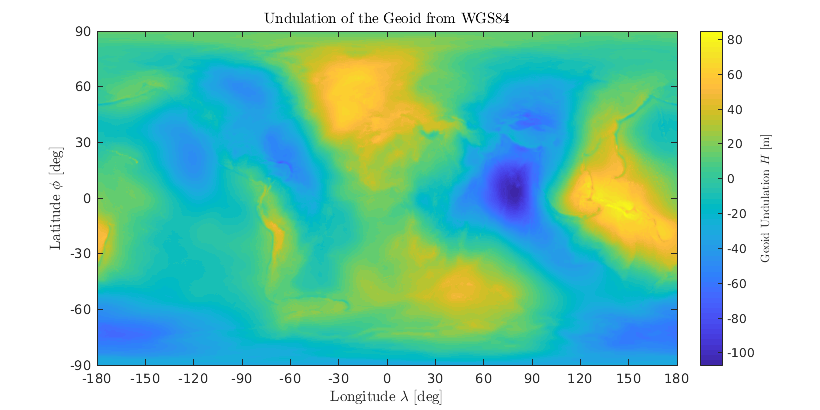
\includegraphics[width=\linewidth]{GeoidUndulationfromWGS84200Contours.png}
	\begin{overpic}[width=\linewidth]{GeoidUndulationfromWGS84200Contours.png}
	\put(28,47.25){\colorbox{white}{Undulation of the Geoid from WGS84}}
	\put(38.5,0.55){\colorbox{white}{\small Longitude $\lambda$ [deg]}}
%	\put(5, 18){\colorbox{white}{\rotatebox{90}{\small Latitude $\phi$ [deg]}}}
	\put(5, 13.5){\colorbox{white}{\rotatebox{90}{\small Geodetic Latitude $\phi$ [deg]}}}
	\put(91.5, 38){\colorbox{white}{\rotatebox{270}{\footnotesize Geoid Undulation $N$ [m]}}}
	
	% Try overlaying ticks
	% x axis
	\put(9.5, 2.9){\colorbox{white}{\scriptsize -$180$}}
	\put(15.25, 2.9){\colorbox{white}{\scriptsize -$150$}}
	\put(21, 2.9){\colorbox{white}{\scriptsize -$120$}}
	\put(27.5, 2.9){\colorbox{white}{\scriptsize -$90$}}
	\put(33.5, 2.9){\colorbox{white}{\scriptsize -$60$}}
	\put(39.35, 2.9){\colorbox{white}{\scriptsize -$30$}}
	\put(46.175, 2.9){\colorbox{white}{\scriptsize $0$}}
	\put(51.5, 2.9){\colorbox{white}{\scriptsize $30$}}
	\put(57.35, 2.9){\colorbox{white}{\scriptsize $60$}}
	\put(63.35, 2.9){\colorbox{white}{\scriptsize $90$}}
	\put(68.8, 2.9){\colorbox{white}{\scriptsize $120$}}
	\put(74.6, 2.9){\colorbox{white}{\scriptsize $150$}}
	\put(80.5, 2.9){\colorbox{white}{\scriptsize $180$}}
	
	% y axis
	\put(7.85, 5.45){\colorbox{white}{\scriptsize -$90$}}
	\put(7.85, 11.75){\colorbox{white}{\scriptsize -$60$}}
	\put(7.85, 18.6){\colorbox{white}{\scriptsize -$30$}}
	\put(9.35, 25.25){\colorbox{white}{\scriptsize $0$}}
	\put(8.5, 32.15){\colorbox{white}{\scriptsize $30$}}
	\put(8.5, 39){\colorbox{white}{\scriptsize $60$}}
	\put(8.5, 45.5){\colorbox{white}{\scriptsize $90$}}
	
	% z axis
	\put(88.3, 6.5){\colorbox{white}{\ssmall -$100$}} % 6.5
	\put(88.3, 10.65){\colorbox{white}{\ssmall -$80$}}
	\put(88.3, 14.9){\colorbox{white}{\ssmall -$60$}}
	\put(88.3, 19.15){\colorbox{white}{\ssmall -$40$}}
	\put(88.3, 23.4){\colorbox{white}{\ssmall -$20$}}
	\put(88.3, 27.75){\colorbox{white}{\ssmall $0$}}
	\put(88.3, 32){\colorbox{white}{\ssmall $20$}}
	\put(88.3, 36.15){\colorbox{white}{\ssmall $40$}}
	\put(88.3, 40.5){\colorbox{white}{\ssmall $60$}}
	\put(88.3, 44.75){\colorbox{white}{\ssmall $80$}}
	\end{overpic}
	\caption{The tide-free EGM2008 geoid undulations from WGS84}
	\label{fig:GeoidUndulationsFromWGS84}
\end{figure}



The displacements of the local topography from the geoid shown in Fig. \ref{fig:LocalTopographyDisplacementFromGeoid} were computed according to (\ref{eq:HeightAboveMSL}) using all harmonic coefficients provided by EGM2008 to obtain a resolution of $2.5' \times 2.5'$. 
\begin{figure}[H]
	\centering
%	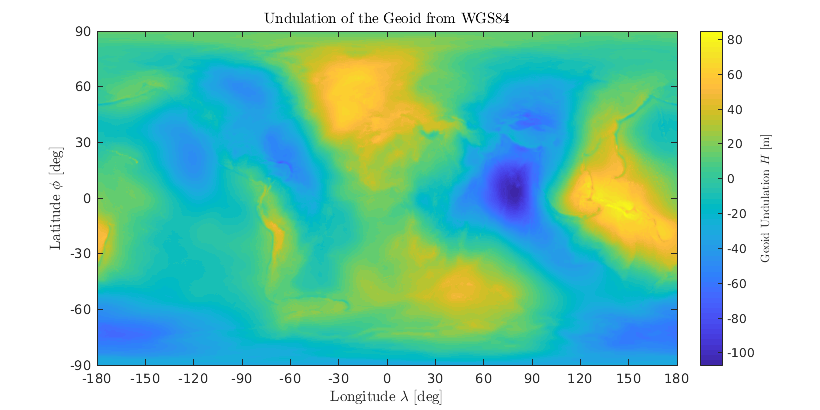
\includegraphics[width=\linewidth]{GeoidUndulationfromWGS84200Contours.png}
	\begin{overpic}[width=\linewidth]{DisplacementOfLocalTopographyFromTheGeoid4.png}
	\put(16.25,47.8){\colorbox{white}{Displacement of Local Topography from the Geoid (MSL)}} %20 w/o "(MSL)"
	\put(38.5,0.55){\colorbox{white}{\small Longitude $\lambda$ [deg]}}
%	\put(5, 18){\colorbox{white}{\rotatebox{90}{\small Latitude $\phi$ [deg]}}}
	\put(5, 13.5){\colorbox{white}{\rotatebox{90}{\small Geodetic Latitude $\phi$ [deg]}}}
	\put(93.5, 41.25){\colorbox{white}{\rotatebox{270}{\footnotesize Topography Displacement $H$ [m]}}}
	
	% Try overlaying ticks
	% x axis
	\put(9.5, 2.9){\colorbox{white}{\scriptsize -$180$}}
	\put(15.25, 2.9){\colorbox{white}{\scriptsize -$150$}}
	\put(21, 2.9){\colorbox{white}{\scriptsize -$120$}}
	\put(27.5, 2.9){\colorbox{white}{\scriptsize -$90$}}
	\put(33.5, 2.9){\colorbox{white}{\scriptsize -$60$}}
	\put(39.35, 2.9){\colorbox{white}{\scriptsize -$30$}}
	\put(46.285, 2.9){\colorbox{white}{\scriptsize $0$}}
	\put(51.7, 2.9){\colorbox{white}{\scriptsize $30$}}
	\put(57.65, 2.9){\colorbox{white}{\scriptsize $60$}}
	\put(63.5, 2.9){\colorbox{white}{\scriptsize $90$}}
	\put(69, 2.9){\colorbox{white}{\scriptsize $120$}}
	\put(74.9, 2.9){\colorbox{white}{\scriptsize $150$}}
	\put(80.5, 2.9){\colorbox{white}{\scriptsize $180$}}
	
	% y axis
	\put(7.85, 5.45){\colorbox{white}{\scriptsize -$90$}}
	\put(7.85, 11.75){\colorbox{white}{\scriptsize -$60$}}
	\put(7.85, 18.6){\colorbox{white}{\scriptsize -$30$}}
	\put(9.35, 25.25){\colorbox{white}{\scriptsize $0$}}
	\put(8.5, 32.25){\colorbox{white}{\scriptsize $30$}}
	\put(8.5, 39){\colorbox{white}{\scriptsize $60$}}
	\put(8.5, 45.5){\colorbox{white}{\scriptsize $90$}}
	
	% z axis
%	\put(88.3, 6.5){\colorbox{white}{\ssmall -$100$}} % 6.5
	\put(88.3, 9.85){\colorbox{white}{\ssmall -$8000$}}
	\put(88.3, 14.7){\colorbox{white}{\ssmall -$6000$}}
	\put(88.3, 19.6){\colorbox{white}{\ssmall -$4000$}}
	\put(88.3, 24.3){\colorbox{white}{\ssmall -$2000$}}
	\put(88.3, 29.25){\colorbox{white}{\ssmall $0$}}
	\put(88.3, 34.2){\colorbox{white}{\ssmall $2000$}}
	\put(88.3, 39){\colorbox{white}{\ssmall $4000$}}
	\put(88.3, 43.8){\colorbox{white}{\ssmall $6000$}}
%	\put(88.3, 44.75){\colorbox{white}{\ssmall $8000$}}
	\end{overpic}
	\caption{The variation of local surface topography from the tide-free geoid}
	\label{fig:LocalTopographyDisplacementFromGeoid}
\end{figure}
\noindent
In accordance with (\ref{eq:ElevationAboveMSL}), the combination (addition) of Figs. \ref{fig:GeoidUndulationsFromWGS84} and \ref{fig:LocalTopographyDisplacementFromGeoid} yields the displacement of Earth's surface (without an ocean) from the WGS84 ellipsoid directly.

The majority of continental area is shown to be near zero (green/blue) since major mountain ranges and the ocean floor largely dominate the scale's extremities. 
As the lowest point on Earth is in the Dead Sea at an elevation of approximately $415$ [\si{\m}] beneath MSL, the ocean's surface (tide-free), which \textit{is} the geoid over open water, can be approximated by setting values on the ocean floor (less than -$415$ [\si{\m}]) to zero. Elevations of Earth's liquid and solid surfaces (ocean and continental) above MSL are therefore in accordance with Fig. \ref{fig:LocalTopographyDisplacementFromGeoidBlack}, which approximates the telluroid.
\begin{figure}[H]
	\centering
%	\begin{overpic}[width=\linewidth]{DisplacementofLocalTopographyfromtheGeoidBoneColorMapSeaLevelBlack.png}
	\begin{overpic}[width=\linewidth]{GeoidUndulationfromWGS84InfernoColorMapMSLisNaN.png}
	% Shown is such that H(H < -415) = NaN and NaN is set to black such that (0,0,0) is actually not on the color bar
	% H(H < -415) = 0 would technically be more correct, but doesn't look as nice as 0 is a bit of grey
	\put(14.25,48.2){\colorbox{white}{Displacement of Continental Topography from the Geoid (MSL)}} %20 w/o "(MSL)"
	\put(39.5,0.55){\colorbox{white}{\small Longitude $\lambda$ [deg]}}
%	\put(5, 18){\colorbox{white}{\rotatebox{90}{\small Latitude $\phi$ [deg]}}}
	\put(5, 13.5){\colorbox{white}{\rotatebox{90}{\small Geodetic Latitude $\phi$ [deg]}}}
	\put(92.8, 40.25){\colorbox{white}{\rotatebox{270}{\footnotesize Topography Displacement $H$ [m]}}}
	
	% Try overlaying ticks
	% x axis
	\put(9.7, 3.1){\colorbox{white}{\scriptsize -$180$}}
	\put(15.5, 3.1){\colorbox{white}{\scriptsize -$150$}}
	\put(21.4, 3.1){\colorbox{white}{\scriptsize -$120$}}
	\put(28.1, 3.1){\colorbox{white}{\scriptsize -$90$}}
	\put(34.2, 3.1){\colorbox{white}{\scriptsize -$60$}}
	\put(40, 3.1){\colorbox{white}{\scriptsize -$30$}}
	\put(47.15, 3.1){\colorbox{white}{\scriptsize $0$}}
	\put(52.65, 3.1){\colorbox{white}{\scriptsize $30$}}
	\put(58.65, 3.1){\colorbox{white}{\scriptsize $60$}}
	\put(64.7, 3.1){\colorbox{white}{\scriptsize $90$}}
	\put(70.2, 3.1){\colorbox{white}{\scriptsize $120$}}
	\put(76.25, 3.1){\colorbox{white}{\scriptsize $150$}}
	\put(81.8, 3.1){\colorbox{white}{\scriptsize $180$}}
	
	% y axis
	\put(8.1, 5.45){\colorbox{white}{\scriptsize -$90$}}
	\put(8.1, 11.8){\colorbox{white}{\scriptsize -$60$}}
	\put(8.1, 18.7){\colorbox{white}{\scriptsize -$30$}}
	\put(9.7, 25.5){\colorbox{white}{\scriptsize $0$}}
	\put(8.8, 32.4){\colorbox{white}{\scriptsize $30$}}
	\put(8.8, 39.3){\colorbox{white}{\scriptsize $60$}} % aligned
	\put(8.8, 45.9){\colorbox{white}{\scriptsize $90$}}
	
	% z axis
	\put(88.2, 7.7){\colorbox{white}{\ssmall $0$}} % 88.2
	\put(88.2, 13.3){\colorbox{white}{\ssmall $1000$}}
	\put(88.2, 18.9){\colorbox{white}{\ssmall $2000$}}
	\put(88.2, 24.4){\colorbox{white}{\ssmall $3000$}}
	\put(88.2, 29.9){\colorbox{white}{\ssmall $4000$}}
	\put(88.2, 35.4){\colorbox{white}{\ssmall $5000$}}
	\put(88.2, 41){\colorbox{white}{\ssmall $6000$}}
	\end{overpic}
	\caption{The variation of local surface topography on the continents from the tide-free EGM2008 geoid. There is no displacement from the geoid on the open ocean by definition.}
	\label{fig:LocalTopographyDisplacementFromGeoidBlack}
\end{figure}

Combining (adding) Fig. \ref{fig:GeoidUndulationsFromWGS84} to Fig. \ref{fig:LocalTopographyDisplacementFromGeoidBlack} furnishes the elevation of Earth's liquid and solid surfaces with respect to the WGS84 ellipsoid. Subtly, the (tide-free) MSL changes globally, which is due simply to the geoid describing mass fluctuations throughout the earth.
\begin{figure}[H]
	\centering
%	\begin{overpic}[width=\linewidth]{DisplacementofLocalTopographyfromtheGeoidBoneColorMapSeaLevelBlackWithGeoidUndulations.png}
	\begin{overpic}[width=\linewidth]{GeoidUndulationfromWGS84InfernoColorMapMSLis0.png}
	% Shown is such that H(H < -415) = NaN and NaN is set to black such that (0,0,0) is actually not on the color bar
	% H(H < -415) = 0 would technically be more correct, but doesn't look as nice as 0 is a bit of grey
	\put(23.6,48.25){\colorbox{white}{Displacement of Earth's Surface from WGS84}} %20 w/o "(MSL)"
	\put(39.5,0.55){\colorbox{white}{\small Longitude $\lambda$ [deg]}}
%	\put(5, 18){\colorbox{white}{\rotatebox{90}{\small Latitude $\phi$ [deg]}}}
	\put(5, 13.5){\colorbox{white}{\rotatebox{90}{\small Geodetic Latitude $\phi$ [deg]}}}
	\put(92.8, 40.25){\colorbox{white}{\rotatebox{270}{\footnotesize Topography Displacement $h$ [m]}}}
	
	% Try overlaying ticks
	% x axis
	\put(9.7, 3.1){\colorbox{white}{\scriptsize -$180$}}
	\put(15.5, 3.1){\colorbox{white}{\scriptsize -$150$}}
	\put(21.4, 3.1){\colorbox{white}{\scriptsize -$120$}}
	\put(28.1, 3.1){\colorbox{white}{\scriptsize -$90$}}
	\put(34.2, 3.1){\colorbox{white}{\scriptsize -$60$}}
	\put(40, 3.1){\colorbox{white}{\scriptsize -$30$}}
	\put(47.15, 3.1){\colorbox{white}{\scriptsize $0$}}
	\put(52.65, 3.1){\colorbox{white}{\scriptsize $30$}}
	\put(58.65, 3.1){\colorbox{white}{\scriptsize $60$}}
	\put(64.7, 3.1){\colorbox{white}{\scriptsize $90$}}
	\put(70.2, 3.1){\colorbox{white}{\scriptsize $120$}}
	\put(76.25, 3.1){\colorbox{white}{\scriptsize $150$}}
	\put(81.8, 3.1){\colorbox{white}{\scriptsize $180$}}
	
	% y axis
	\put(8.1, 5.45){\colorbox{white}{\scriptsize -$90$}}
	\put(8.1, 11.8){\colorbox{white}{\scriptsize -$60$}}
	\put(8.1, 18.6){\colorbox{white}{\scriptsize -$30$}}
	\put(9.7, 25.5){\colorbox{white}{\scriptsize $0$}}
	\put(8.8, 32.45){\colorbox{white}{\scriptsize $30$}}
	\put(8.8, 39.2){\colorbox{white}{\scriptsize $60$}} % aligned
	\put(8.8, 45.8){\colorbox{white}{\scriptsize $90$}}
	
	% z axis
	\put(88.2, 7.9){\colorbox{white}{\ssmall $0$}} % 88.2
	\put(88.2, 13.3){\colorbox{white}{\ssmall $1000$}}
	\put(88.2, 18.9){\colorbox{white}{\ssmall $2000$}}
	\put(88.2, 24.4){\colorbox{white}{\ssmall $3000$}}
	\put(88.2, 29.9){\colorbox{white}{\ssmall $4000$}}
	\put(88.2, 35.5){\colorbox{white}{\ssmall $5000$}}
	\put(88.2, 41){\colorbox{white}{\ssmall $6000$}}
	\end{overpic}
	\caption{The variation of local surface topography (ocean and land) over Earth's surface from WGS84}
	\label{fig:LocalTopographyDisplacementFromWGS84}
\end{figure}
\noindent
The variation of MSL over the oceans with respect to WGS84 is within Fig. \ref{fig:GeoidUndulationsFromWGS84} as this variation is what defines the geoid. For clarity, however, Fig. \ref{fig:MSLDisplacementFromWGS84}  overlays this variation with the continents to show only how the tide-free ocean's MSL varies over the surface of Earth.
\begin{figure}[H]
	\centering
	\begin{overpic}[width=\linewidth]{GeoidUndulationfromWGS84InfernoColorMapLand(-415)isNaN.png}
	% Shown is such that H(H < -415) = NaN and NaN is set to black such that (0,0,0) is actually not on the color bar
	% H(H < -415) = 0 would technically be more correct, but doesn't look as nice as 0 is a bit of grey
	\put(22.6,48.25){\colorbox{white}{Displacement of the Geoid (MSL) from WGS84}} %20 w/o "(MSL)"
	\put(39.5,0.55){\colorbox{white}{\small Longitude $\lambda$ [deg]}}
%	\put(5, 18){\colorbox{white}{\rotatebox{90}{\small Latitude $\phi$ [deg]}}}
	\put(5, 13.5){\colorbox{white}{\rotatebox{90}{\small Geodetic Latitude $\phi$ [deg]}}}
	\put(92.6, 40.25){\colorbox{white}{\rotatebox{270}{\footnotesize Topography Displacement $h$ [m]}}}
	
	% Try overlaying ticks
	% x axis
	\put(9.7, 3.1){\colorbox{white}{\scriptsize -$180$}}
	\put(15.5, 3.1){\colorbox{white}{\scriptsize -$150$}}
	\put(21.4, 3.1){\colorbox{white}{\scriptsize -$120$}}
	\put(28.1, 3.1){\colorbox{white}{\scriptsize -$90$}}
	\put(34.2, 3.1){\colorbox{white}{\scriptsize -$60$}}
	\put(40, 3.1){\colorbox{white}{\scriptsize -$30$}}
	\put(47.15, 3.1){\colorbox{white}{\scriptsize $0$}}
	\put(52.65, 3.1){\colorbox{white}{\scriptsize $30$}}
	\put(58.65, 3.1){\colorbox{white}{\scriptsize $60$}}
	\put(64.7, 3.1){\colorbox{white}{\scriptsize $90$}}
	\put(70.2, 3.1){\colorbox{white}{\scriptsize $120$}}
	\put(76.25, 3.1){\colorbox{white}{\scriptsize $150$}}
	\put(81.8, 3.1){\colorbox{white}{\scriptsize $180$}}
	
	% y axis
	\put(8.1, 5.45){\colorbox{white}{\scriptsize -$90$}}
	\put(8.1, 11.8){\colorbox{white}{\scriptsize -$60$}}
	\put(8.1, 18.6){\colorbox{white}{\scriptsize -$30$}}
	\put(9.7, 25.5){\colorbox{white}{\scriptsize $0$}}
	\put(8.8, 32.45){\colorbox{white}{\scriptsize $30$}}
	\put(8.8, 39.2){\colorbox{white}{\scriptsize $60$}} % aligned
	\put(8.8, 45.8){\colorbox{white}{\scriptsize $90$}}
	
	% z axis
	\put(88.2, 6.5){\colorbox{white}{\ssmall -$100$}} % 6.5
	\put(88.2, 10.8){\colorbox{white}{\ssmall -$80$}}
	\put(88.2, 15.2){\colorbox{white}{\ssmall -$60$}}
	\put(88.2, 19.6){\colorbox{white}{\ssmall -$40$}}
	\put(88.2, 24){\colorbox{white}{\ssmall -$20$}}
	\put(88.2, 28.3){\colorbox{white}{\ssmall $0$}}
	\put(88.2, 32.7){\colorbox{white}{\ssmall $20$}}
	\put(88.2, 37.1){\colorbox{white}{\ssmall $40$}}
	\put(88.2, 41.45){\colorbox{white}{\ssmall $60$}}
	\put(88.2, 45.9){\colorbox{white}{\ssmall $80$}}
	\end{overpic}
	\caption{The variation of MSL (tide-free EGM2008 geoid) over the oceans with respect to WGS84. This figure is exactly the same as Fig. \ref{fig:GeoidUndulationsFromWGS84} but with a different coloring and overlaid continents. Elevations exceeding the Dead Sea are ignored -- some continental areas may appear fat as such.}
	\label{fig:MSLDisplacementFromWGS84}
\end{figure}

The topography of the continental United States with respect to the EGM2008 tide-free geoid (MSL) is shown in Fig. \ref{fig:USATopographyWRTMSL}.
\begin{figure}[H]
	\centering
	\begin{overpic}[width=\linewidth]{DisplacementofLocalTopographyfromWGS84PlottedonSphere(geocentricLat)4.png}
	\put(29,58.25){\colorbox{white}{Displacement of Topography from MSL}}
	\put(33.25,55.25){\colorbox{white}{in the United States of America}}
	\put(45,7.55){\colorbox{white}{\small Longitude $\lambda$ [deg]}}
%	\put(5, 13.5){\colorbox{white}{\rotatebox{75}{\small Geodetic Latitude $\phi$ [deg]}}}
	\put(6, 29.5){\rotatebox{70.5}{\small Geodetic Latitude $\phi$ [deg]}} %74.25 aligned on edge
	\put(13, 6.1){{\setlength{\fboxsep}{0pt}\colorbox{white}{\footnotesize Topography Displacement $H$ [m]}}} %61 right
	
	% Longitudes
	\put(16.5, 15){\colorbox{white}{\rotatebox{-13.5}{\textcolor{white}{\ssmall $120^\circ$}}}}
	\put(19, 14){\colorbox{white}{\rotatebox{-13.5}{\textcolor{white}{\ssmall W}}}}
	\put(16.5, 15){\rotatebox{-13.5}{\ssmall $120^\circ$W}} % Needs own colorbox, too tilted
	\put(30, 11.75){\colorbox{white}{\rotatebox{-11.5}{\ssmall $110^\circ$W}}}
	\put(43.75, 10.2){\colorbox{white}{\rotatebox{-1.5}{\ssmall $100^\circ$W}}}
	\put(58.25, 10.25){\colorbox{white}{\rotatebox{2}{\ssmall $90^\circ$W}}}
	\put(72, 11.5){\colorbox{white}{\rotatebox{9}{\ssmall $80^\circ$W}}}
	\put(85.5, 14.25){\colorbox{white}{\rotatebox{15}{\ssmall $70^\circ$W}}}
	
	% Latitudes
	\put(10.75, 28.75){\colorbox{white}{\rotatebox{-17}{\textcolor{white}{\ssmall $30^\circ$}}}}
	\put(15, 42.55){\colorbox{white}{\rotatebox{-17}{\textcolor{white}{\ssmall $40^\circ$}}}}
	\put(19.5, 56.6){\colorbox{white}{\rotatebox{-17}{\textcolor{white}{\ssmall $50^\circ$}}}}
	% None can handle colorboxes
	\put(10.75, 28.75){\rotatebox{-17}{\ssmall $30^\circ$N}}
	\put(15, 42.55){\rotatebox{-17}{\ssmall $40^\circ$N}}
	\put(19.5, 56.6){\rotatebox{-17}{\ssmall $50^\circ$N}}
	
	% Colorbar
	\put(13.75, 1.2){\colorbox{white}{\ssmall $0$}} %13.75
	\put(22.8, 1.2){\colorbox{white}{\ssmall $500$}}
	\put(32.25, 1.2){\colorbox{white}{\ssmall $1000$}}
	\put(42, 1.2){\colorbox{white}{\ssmall $1500$}}
	\put(52, 1.2){\colorbox{white}{\ssmall $2000$}}
	\put(61.75, 1.2){\colorbox{white}{\ssmall $2500$}}
	\put(71.5, 1.2){\colorbox{white}{\ssmall $3000$}}
	\put(81.5, 1.2){\colorbox{white}{\ssmall $3500$}}
	\end{overpic}
	\caption{The topography of the continental United States with respect to MSL overlaid with the 48 continguous state borders and part of the North American coastline.}
	\label{fig:USATopographyWRTMSL}
\end{figure}

Since the geoid varies by no more than 105 meters from the WGS84 ellipsoid, a rough approximation of (\ref{eq:ElevationAboveMSL}) yields, especially for very high altitudes, that $H \sim h$. Thus, a height $h$ above the ellipsoid or a height $H$ above MSL may be used for determining atmospheric properties without generating large errors, though this choice should remain consistent throughout as to, in general, avoid discontinuities in atmospheric conditions. That is, an elevation $H$ above MSL may be used at low altitudes and switched to an elevation $h$ above the ellipsoid if passing over a region where the geoid undulation is truly zero (or close enough). Doing so relaxes intensive computations while maintaining a continuously modelled atmosphere.

It is noted that the highest tabulated elevation above MSL (in accordance with Fig. \ref{fig:LocalTopographyDisplacementFromGeoidBlack}) is 6959.9 meters whereas the summit of Mount Everest is 8848 meters (29029 feet). Likewise, the highest peak in the continental United States (in accordance with Fig. \ref{fig:USATopographyWRTMSL}) is in California atop Mount Whitney at 4418 meters (14494 feet) above MSL. According to the figure, the highest peak in the continental United States is tabulated as 3837.3 meters (12590 feet). These errors are likely due because of grid spacing. The selected geodetic coordinates making up the grids either missed the peaks of Mount Everest and Mount Whitney (amoung others surely) because of its ``lacking'' $2.5' \times 2.5'$ resolution, or simply because of the limiting resolution that the coefficients provided from GRACE can acquire.
The case seems to be the latter; inserting the coordinates of Mount Everest's peak and checking in its surrounding area supplies no such extreme, and likewise for Mount Whitney.


\section{Atmospheric Model}

Atmospheric properties are perhaps one of the most difficult aspects of the earth to model and predict accurately at any given time because of its naturally almost chaotic and quickly evolving behavior. For this reason, a \textit{standard atmosphere} may be established, representing not real, instantaneous atmospheric properties, but rather standardized conditions that are generally accepted by the scientific community.
\subsection{Gas Properties}
In most cases concerning the atmosphere, air is treated as an \textit{ideal gas} (as opposed to a real gas) so that the \textit{ideal gas law}, serving as the \textit{equation of state} (which relates air pressure $p$, air temperature $T$, and air density $\rho$), is obeyed.
\begin{equation}
p = \rho R T \label{eq:IdealGasLaw}
\end{equation}
Here, $R$ is the specific gas constant defined by the molecular weight $\mathcal{M}$ of the gas with the universal gas constant $\mathcal{R}$, which is itself the product of fundamental quantities (Avogadro and Boltzmann constants).

\begin{equation}
\mathcal{R} = N_{\!A} \hspace{0.225ex} k_B \approx \num{8.31446261815324}\ \si{[\J / \K \,\mol]}
\end{equation}
The continuously-ongoing process of atmospheric motion and mixing with itself throughout the world can be leveraged to say that the composition of air close to the surface, which is a mixture of gases, is approximately uniform everywhere. However, this composition changes in time
%, perhaps most significantly being carbon dioxide, 
which affects, albeit slightly, the gas constant of air defined
\begin{equation}
R = \mathcal{R} / \mathcal{M}. \label{eq:gasConstant}
\end{equation}
Thus, most recent atmospheric data is apt to give a most current value of air's gas constant. Obtaining a single value for the gas constant of ``the air'' represents what is like a global average air, though it may be interpreted also in a pointwise sense. In any case, the type of considered air is \textit{dry air} and does not take into account local variations of (particularly) humidity at any location. Regardless of details involving the ``exact'' composition of air, its gas constant remains approximately constant up to the mesopause (an elevation of about 90 [\si{\km}] above sea level) and is
\begin{equation}
R \sim 287 \ [\si{\J / \kg\,\K}].
\end{equation}
Specifying the composition of air to gain an accurate molecular weight is really fine-tuning the gas constant's decimals.

By physical intuition, every gas has a measure of how resistant it is to changing its temperature when supplied a heat source to do so. Two such quantities realize this resistance in the form of how much energy must be supplied to produce a unit change in the gas's temperature --- the specific heat capacity at constant pressure $c_p$ and the specific heat capacity at constant volume $c_v$ (note the subscript $v$ despite the typical denotation of volume as $V$). 
The term ``specific'' here indicates that quantities are measured per kilogram. Thus, unit masses of gas are implied and the density is consequently the inverse of the containing volume, termed the specific volume $v$.
The quantity $c_v$ is therefore actually a statement about the gas's specific heat capacity at constant density.
Obviously, there is no need for a quantity describing specific heat capacity at constant temperature.
It is a fact that these two quantities, $c_p$ and $c_v$, for any gas are mainly dependent upon temperature (weakly dependent upon pressure) and both increase along with temperature.

A ratio of the two (specific) heat capacity ratios, denoted $\gamma$ (not to be confused with the normal gravity $\gamma$) is defined
\begin{equation}
\gamma = c_p / c_v. \label{eq:SpecificHeatRatio}
\end{equation}
Thus, $\gamma$, called the \textit{heat capacity ratio}, is dependent upon temperature. Mayer's relation for an ideal gas provides further insight into how these quantities relate to each other.
\begin{equation}
R = c_p - c_v. \label{eq:MayersEq}
\end{equation}
The gas constant $R$ is obviously a positive quantity as indicated by (\ref{eq:gasConstant}), but perhaps less apparent, it is \textit{independent} of temperature. The respective conclusions are therefore $\gamma > 1$ and (\ref{eq:MayersEq}) is true everywhere.
%
Since both specific heat capacities $c_p$ and $c_v$ increase with temperature but maintain a constant difference, the heat capacity ratio $\gamma$ decreases towards unity with increasing temperature as indicated by Fig. \ref{fig:AirHeatCapacityRatioGraph}.
\begin{figure}[H]%b!
\centering
\begin{tikzpicture}
	\begin{axis}[
width=3.229in,
height=2.461in,
at={(0.542in,0.43in)},
scale only axis,
%unbounded coords=jump,
xmin=200,
xmax=1300,
xtick={200,350,...,1250},
%xticklabels={{-90},{},{-60},{},{-30},{},{0},{},{30},{},{60},{},{90}},
xlabel style={font=\color{white!15!black}},
xlabel={Temperature $T$ [\si{\K}]},
%ymin=1.3125,
%ymax=1.4075,
ytick={1.32,1.33,...,1.41},
%yticklabels={{-90},{},{-60},{},{-30},{},{0},{},{30},{},{60},{},{90}},
ylabel style={font=\color{white!15!black}},
ylabel={Heat Capacity Ratio $\gamma$},
axis background/.style={fill=white},
title style={font=\bfseries},
title={Heat Capacity Ratio of Dry Air},
xmajorgrids,
ymajorgrids,
]
\addplot[mark=x,smooth] coordinates {
		(233.15, 	1.401)
		(253.15, 	1.401)
		(273.15, 	1.401)
		(278.15, 	1.401)
		(283.15, 	1.401)
		(288.15, 	1.401)
		(293.15, 	1.401)
		(298.15, 	1.401)
		(303.15, 	1.400)
		(313.15, 	1.400)
		(323.15, 	1.400)
		(333.15, 	1.399)
		(343.15, 	1.399)
		(353.15, 	1.399)
		(363.15, 	1.398)
		(373.15, 	1.397)
		(473.15, 	1.390)
		(573.15, 	1.379)
		(673.15, 	1.368)
		(773.15, 	1.357)
		(1273.15, 	1.321)
	};
\end{axis}
\end{tikzpicture}
\caption{The variation of air's heat capacity ratio on temperature (neglecting variations with pressure) [engineering toolbox].}
\label{fig:AirHeatCapacityRatioGraph}
\end{figure}

Gases obeying the ideal gas law are said to be \textit{thermally perfect}, and gases obeying a constant heat capacity ratio $\gamma$, at least in some specified range of temperature, are said to be \textit{calorically perfect} (in that temperature range). Gases that are both thermally perfect and calorically perfect are \textit{ideal}, which of course is an idealization of reality. Real gases are not perfect and consequently obey a different equation of state than the ideal gas law. Many such models exist, like van der Waals or Redlich-Kwong, which necessarily change Mayer's result (\ref{eq:MayersEq}) to its general form
\begin{equation}
-T \frac{(\partial p / \partial T)_v^2}{(\partial p / \partial v)_T} = c_p - c_v.
\end{equation}
As an example, the original Redlich-Kwong equation of state yields
\begin{align}
p &= \frac{RT}{v - b} - \frac{a}{T^{1/2} v (v + b)} \qquad (\rho = 1 / v) \\
a &= \frac{R^2 \,{T_c}^{\!5/2} / p_c}{9\,(2^{1/3} - 1)} \\
b &= \frac{R \,T_c \,/ p_c}{3 / (2^{1/3} - 1)},
\end{align}
where $p_c$ and $T_c$ are the pressure and temperature critical points respectively,
for which the difference in specific heat capacities becomes
\begin{align}
c_p - c_v &= \left(\frac{R}{v - b} + \frac{1}{2}\frac{a}{T^{3/2} v (v+b)}\right)^{\!2} / \left(\frac{R}{(v - b)^2} - \frac{a (2v + b)}{T^{3/2} v (v + b)^2}\right).
\end{align}
If $a$, representing the correction for the molecular potential attraction, and $b$, representing a correction to specific volume, are both set to zero, then the ideal gas law is recovered.

Treating air as calorically imperfect requires a quantum mechanical inspection for a full description of its behavior. The atoms within experience changes in the amount of degrees of freedom which are unlocked by increasing temperature. Merely having three spatial dimensions in which space exists and the impossibility of reaching absolute zero is enough to unlock the first mode for all molecules consisting of three degrees of freedom  --- translation. The other two modes (rotation and vibration) at such low temperatures are unactivated, or \textit{frozen}. 

The rotational mode is fully activated shortly after absolute zero (50 [\si{\K}] or so), which unlocks an amount of degrees of freedom dependent on the kind of molecule.
%
Monotonic molecules have no other modes than translation. Molecules arranged in a line (linear molecules, all bonds are 180$^\circ$ apart) unlock two additional degrees of freedom whereas nonlinear molecules (all other molecules that are not monotonic and not linear) unlock three.

The vibrational mode requires high temperatures to fully activate. A molecule consisting of $N$ atoms unlocks an additional $3N - 5$ degrees of freedom if it is linear (to the 5 it already had) and $3N - 6$ otherwise (to the 6 it already had) [Heat Transfer Physics pg. 397]. Of course, monotonic atoms have no vibrational mode, so they still have only 3 degrees of freedom.

The heat capacity ratio $\gamma$ can be written in terms of these amounts of degrees of freedom at low temperatures (such that the vibrational mode has not yet become too active) to good approximation as
\begin{equation}
\gamma \sim 1 + \frac{2}{\mathrm{degrees\,of\,freedom}}.
\end{equation}
As expected then by Fig. \ref{fig:AirHeatCapacityRatioGraph}, air (a \textit{mixture} largely composed of diatomic molecules \ch{N2} and \ch{O2}) contains 5 degrees of freedom, so at these temperatures,
\begin{equation}
\gamma \sim 1.4. \label{eq:AirHeatRatio1.4}
\end{equation}

As temperatures increase, however, the specific heats should properly be written as functions of temperature. If the vibrations are considered as a simple quantum harmonic oscillator, then the according relations follow the kinetic theory of gases [NASA GRC Calorically Imperfect Gas]
\begin{align}
c_p &= {c_p}_{\text{cal.perfect}} \left(1 + (1 - 1 / \gamma_{\text{perfect}}) \left(\frac{\Theta}{T}\right)^{\!2} \frac{\mathrm{e}^{\Theta / T}}{(\mathrm{e}^{\Theta / T} - 1)^2}\right) \\
c_v &= {c_v}_{\text{cal.perfect}} \left(1 - (1 - \gamma_{\text{perfect}}) \left(\frac{\Theta}{T}\right)^{\!2} \frac{\mathrm{e}^{\Theta / T}}{(\mathrm{e}^{\Theta / T} - 1)^2}\right) \\
\gamma &= 1 + \frac{\displaystyle\gamma_{\text{perfect}} - 1}{\displaystyle1 + (\gamma_{\text{perfect}} - 1) \left(\frac{\Theta}{T}\right)^{\!2} \frac{\mathrm{e}^{\Theta / T}}{(\mathrm{e}^{\Theta / T} - 1)^2}}.
\end{align}
The quantities ${c_p}_{\text{cal.perfect}}$ and ${c_v}_{\text{cal.perfect}}$ are the specific heat capacities of the gas if it were calorically perfect (i.e., if the heat capacity ratio were constant in temperature) corresponding with the constant value $\gamma_{\text{perfect}}$. For air, the value (\ref{eq:AirHeatRatio1.4}) may be used comfortably as the perfect ratio. The quantity $\Theta$ is the scale temperature set to 5500 [$^\circ\mathrm{R}$], or
\begin{equation}
\Theta = \frac{5}{9} \cdot 5500 \sim 3056 \ [\si{\K}].
\end{equation}
These relations provide a functional description of gas characteristics in temperature and nicely approach back to the perfect values for $T \ll \Theta$. Though, they should be used with the possibility of computational overflows in mind due to the nature of exponentiating several thousand (in the event that temperature drops too low).

Whether thermally and/or calorically imperfect or perfect, the speed of a sound wave, or \textit{speed of sound} denoted $a$ (not to be confused with the semi-major axis of Earth's ellipsoid $a$), travels through the gas according to
\begin{equation}
a^2 = \gamma \frac{\partial p}{\partial \rho}. \label{eq:SpeedOfSound}
\end{equation}
A thermally perfect gas (obeying the ideal gas law) therefore transmits sound at speed
\begin{equation}
a = \sqrt{\gamma R T} \label{eq:SpeedOfSoundIdeal}
\end{equation}
whereas a thermally imperfect gas otherwise transmits sound depending on its equation of state (van der Waals, etc.). The speed of sound at sea level, where $\gamma = 1.4$, $R = 287 \ [\si{\J/\kg\,\K}]$, and $T = 59\ [^\circ\mathrm{F}]$, is therefore
\begin{equation}
a_{059} \sim 340 \ [\si{\m/\s}].
\end{equation}

The kinetic theory of gases gives implications as to how (dynamic) viscosity, denoted $\mu$, should roughly behave. Perhaps the most fundamental model which poses the hardest assumptions on the gas is that of atoms made of solid, perfectly elastic spheres of mass $m$ and diameter $\sigma$. The corresponding viscosity is
\begin{equation}
\mu = \frac{1.016 \cdot 5}{16 \,\sigma^2} \sqrt{m k_B T / \pi}, \qquad (m = \mathcal{M} / N_A).
\end{equation}
Thus, the viscosity of a gas under this model \textit{increases only with temperature as $\mu \propto T^{1/2}$} (liquids typically decrease with increasing temperature). Though simple, this viscosity power law model grows too slowly to match measured data and hence is not a very good description of viscosity.

Sutherland published his model in 1893, coined \textit{Sutherland's Law}, which is consistent with the kinetic theory of gases. It is realized by utilizing weakly attracting intermolecular forces sourced from a potential model for solid spheres of mass $m$ and diameter $\sigma$. The viscosity is written
\begin{equation}
\mu = \frac{5}{16\,\sigma^2} \frac{\sqrt{m k_B T / \pi}}{1 + S / T} = \mu_0 \left(\frac{T}{T_0}\right)^{\!3/2} \frac{T_0 + S}{T + S}.
\end{equation}
Thus, a referenced (measured) viscosity $\mu_0$ at temperature $T_0$ defines the viscosity as a function of temperature and parameter $S$. For air,
\begin{align}
\mu_0 = 0.00001716 \ [\si{\kg / \m\,\s}] && T_0 = 273.15 \ [\si{\K}] && S = 110.4 \ [\si{\K}].
\end{align}
The region of validity for Sutherland's law for \ch{N2} and \ch{O2} falls between 290 and 1100 [\si{\K}] whereas for \ch{Ar}, the range is merely 290 to 375 [\si{\K}]. Dry air is therefore properly limited to the range of \ch{Ar}, though it may be extended to 1100 [\si{\K}] since \ch{Ar} makes up such a trace amount of air in comparison.
Sutherland's law, however, is disputed as to whether it actually gives good results or not.

The Lennard-Jones potential provides a viscosity through the kinetic theory of gases for solid spheres written
\begin{equation}
\mu = \frac{5}{16\,\sigma^2} \frac{\sqrt{m k_B T / \pi}}{\Omega(T)} \overset{?}{=} \mu_0 \left(\frac{T}{T_0}\right)^{\!\!1/2} \frac{\Omega(T_0)}{\Omega(T)},
\end{equation}
where $\Omega$ is called the \textit{collision integral}, which is determined by the expression of the potential. Much like other models (except Sutherland, oddly), the collision integral for Lennard-Jones is not expressible in terms of elementary functions, but is well approximated by
\begin{align}
\Omega(T) \sim 1.16145 \,{T^*}^{-0.14874} + 0.52487 \,\mathrm{e}^{\!-0.77320 \,T^*} + 2.16178 \,\mathrm{e}^{\!-2.43787 \,T^*}, && \left(T^* = \frac{k_B T}{\epsilon}\right),
\end{align}
where $\sigma$ and $\epsilon$ are both constants determined by experiment. These values for various gases commonly found in the atmosphere are tabulated below in Tab. \ref{fig:LennardJonesGasParams}.
\begin{table}[H]
\centering
\caption{Lennard-Jones gas parameters}
\label{fig:LennardJonesGasParams}
\begin{tabular}{c S[table-format=1.3] S[table-format=3.1, table-space-text-pre=1/, table-align-text-pre=false]}
\toprule
{Gas} & {\specialcell{Molecular Diameter \\ $\sigma$ (\si{\angstrom})}} & {\specialcell{Temperature Scale \\ $k_B / \epsilon$ (\si{1/\K})}} \\ \midrule
Dry Air & 3.617 & {1/}97.0 \\
Helium & 2.576 & {1/}10.2 \\
Hydrogen & 2.915 & {1/}38.0 \\
Argon & 3.432 & {1/}122.4 \\
Nitrogen & 3.667 & {1/}99.8 \\
Oxygen & 3.433 & {1/}113.0 \\
Carbon dioxide & 3.996 & {1/}190.0 \\
Methane & 3.780 & {1/}154.0 \\ \bottomrule
\end{tabular}
\end{table}
Despite Lennard-Jones being derived with solid spheres playing the role of atoms, this representation of the viscosity realizes an average deviation from the measured gas viscosity within 0.064\% for the temperature ranges $0.3 < T^* < 100$. Thus, the model does well in describing nonspherical atoms too. [Temperature\_dependence\_of\_viscosity wikipedia]

Upon choosing a model of the dynamic viscosity $\mu$, the \textit{kinematic viscosity} $\nu$ is then defined
\begin{equation}
\nu = \mu / \rho. \label{eq:KinetmaticViscosityDef}
\end{equation}
Though still a valid gas property, the kinetic viscosity plays no role in building a standard atmosphere. Its main feature lies in aerodynamics, but is included here to have both kinds of viscosities together for reference.

\subsection{Layers of the Atmosphere}
The real atmosphere is divided into a few basic layers separated by the behavior of air temperature --- the troposphere, stratosphere, mesosphere, thermosphere, and exosphere. The ionosphere and magnetosphere are also regions of the atmosphere, but they have more specialized roles than separating temperature behaviors.
%(which spans across the mesosphere, thermosphere, and into the exosphere). These layers 
\subsubsection{The Troposphere}
The troposphere is the most dense atmospheric region extending from Earth's surface to about $8\hspace{0.5ex}$--$\hspace{0.4ex}10$ [\si{\km}] at the poles and $14\hspace{0.5ex}$--$\hspace{0.5ex}18$ [\si{\km}] along the equator. It is characterized by a \textit{reduction} of air temperature as above-ground altitude increases. Most of all weather occurs in the troposphere and also usually provides the flight ceiling for commercial planes. The upper-most region of the troposphere is called the tropopause and borders along the bottom of the stratosphere.

\subsubsection{The Stratosphere}
The stratosphere extends from the tropopause up to about $50$ $[\si{\km}]$ and is characterized by an \textit{increase} in air temperature with rising altitude. This increase of temperature is usually why commercial aircraft are often flown beneath $12$ [\si{\km}] (40,000 [$\mathrm{ft}$]) altitude. The stratosphere is what contains the ozone layer which absorbs and scatters most ultraviolet radiation incoming from the sun. The stratopause is defined near the top of the stratosphere ($50\hspace{0.5ex}$--$\hspace{0.5ex}55$ [\si{\km}]) which serves as the boundary between it and the mesosphere.

\subsubsection{The Mesosphere}
The mesosphere begins from the stratopause and extends to about $85$ $[\si{\km}]$ characterized by, again, a \textit{decrease} in air temperature with rising altitude. The upper part of the mesosphere (the mesopause) experiences the coldest temperatures in the atmosphere reaching so low as $170\hspace{0.5ex}$--$\hspace{0.5ex}180$ [\si{\K}] ($-135$ to $-155$ [$^\circ\mathrm{F}$]) at around $85$ [\si{\km}] and $100$ [\si{\km}] altitude. Meteors burn up throughout the mesosphere.

\subsubsection{The Thermosphere}
The thermosphere is the continuation from the mesopause extending up to about $600$ [\si{\km}] in which air temperature \textit{increases} again with increasing altitude. Though the thermosphere's end at $600$ [\si{\km}] is often taken as standard, the gas within expands a considerable amount due to solar heating so the thermosphere's boundary above any fixed point on Earth's surface is highly time-dependent ranging between $500\hspace{0.5ex}$--$\hspace{0.5ex}1000$ [\si{\km}].
And despite ``air'' (really, just gas now) temperatures soaring up as much as $2000\hspace{0.5ex}$--$\hspace{0.5ex}2800$ [\si{\K}] (3,140\hspace{0.5ex}--\hspace{0.5ex}4,580 [$^\circ\mathrm{F}$]), the density is so low throughout that an object in this region receives hardly any heat transfer (from the gas) and thus does \textit{not} experience these kinds of temperatures.
Aurorae and LEO satellites exist in the thermosphere. The upper-most region is called the thermopause which serves as the boundary between the thermosphere and the exosphere.

\subsubsection{The Exosphere}
The exosphere is the final atmospheric layer (though some consider the thermosphere the final layer) in which gas molecules are so diffuse that they hardly interact with each other, follow orbital trajectories, and sometimes escape from the earth system into the ``true'' vacuum of space. As such, there is no solid boundary separating Earth's atmosphere from where space begins.

\subsubsection{Special Regions}
The K\'{a}rm\'{a}n Line, defined at $100$ [\si{\km}] (in the \textit{thermosphere}), is widely recognized as a boundary for the beginning of space where the study of astronautics begins to dominate over aeronautics. In comparison, some estimates for the ``end'' of the exosphere extend out to 10,000 [\si{\km}] and even 100,000--180,000 [\si{\km}] above Earth's surface. To place these heights into perspective, the moon's orbital radius about the earth is around 384,000 [\si{\km}].

The ionosphere is a special region of the atmosphere reaching from about $48$ [\si{\km}] to about $965$ [\si{\km}] above Earth's surface [nasa.gov atmosphere-layers2]. \textit{This region overlaps the stratopause, mesosphere, and thermosphere}, and consequently varies in height along with the thermosphere. Further, the ionosphere is divided into three subregions --- D, E, and F --- based on the absorbed wavelength of incoming solar radiation. In all subregions however, atoms are ionized by solar radiation and then provide the interesting property of reflecting radio waves, thus providing the possibility of global radio communication [scied.ucar.edu, nasa.gov atmosphere-layers2].

The magnetosphere is another special region characterized by ions and free electrons being dominated by Earth's magnetic field, a process that is highly dependent upon Earth's internal activity and solar activity. Unlike the atmospheric regions, the actual profile of the magnetosphere does not resemble a sphere at all, but rather the flow field resulting from the placement of a sphere in supersonic flow. The two main channels of ion and electron travel are termed the Van Allen belts which are located about 3,000 [\si{\km}] and 16,000 [\si{\km}] above the earth's surface.

As mentioned earlier, the earth's atmosphere near the surface is regarded as evenly mixed and distributed due to never-ending turbulent mixing. The region in which this homogeneity is true is called the \textit{homosphere}. Accordingly, the \textit{heterosphere} is the region above the homosphere with strong and ordered molecular diffusion. 
The homosphere and heterosphere are separated by a boundary called the \textit{turbopause}, which is located close to the mesopause about $110$ [\si{\km}] above Earth's surface.
%% and the boundary separating this well-mixed air with diffuse 

\subsection{Sourcing a Standard Atmosphere}
The atmosphere at lower altitudes (not dominated by solar radiation, gravitational/magnetic attraction, etc.) has another governing relation in addition to the equation of state (\ref{eq:IdealGasLaw}). Free air in equilibrium obeys the \textit{hydrostatic equation}
\begin{equation}
\frac{\partial p}{\partial h} = -\rho g, \label{eq:HydrostaticEq}
% \implies p = \int_h^\infty \rho g \, dh'
\end{equation}
%\begin{figure}[b]
%\centering
%\tdplotsetmaincoords{70}{110}
%\begin{tikzpicture}[tdplot_main_coords, scale = 4]
%% Define pressure box side lengths
%\pgfmathsetmacro{\s}{0.25}
%% Draw axis
%%\draw[dashed] (0,0,0) -- (\s,0,0);
%%\draw[dashed] (0,0,0) -- (0,\s,0);
%%\draw[dashed] (0,0,0) -- (0,0,\s);
%%% Continue axes
%%\draw[->,>=stealth,black] (\s,0,0) -- (2.5*\s,0,0) node[right]{$x$};
%%\draw[->,>=stealth,black] (0,\s,0) -- (0,2.5*\s,0) node[right]{$y$};
%%\draw[->,>=stealth,black] (0,0,\s) -- (0,0,2.5*\s) node[left]{$z$};
%
%\draw[dashed] (-\s,-\s,-\s) -- (\s,-\s,-\s);
%\draw[dashed] (-\s,-\s,-\s) -- (-\s,\s,-\s);
%\draw[dashed] (-\s,-\s,-\s) -- (-\s,-\s,\s);
%%
%\draw[->,>=latex,black] (\s,-\s,-\s) -- (1.5*\s,-\s,-\s) node[anchor=north east]{$x$};
%\draw[->,>=latex,black] (-\s,\s,-\s) -- (-\s,1.5*\s,-\s) node[right]{$y$};
%\draw[->,>=latex,black] (-\s,-\s,\s) -- (-\s,-\s,1.5*\s) node[left]{$h$};
%
%% Draw pressure box
%% Front face
%\draw (\s,-\s,-\s) -- (\s,\s,-\s) node[pos=0.4, below]{$dy$} -- (\s,\s,\s) -- (\s,-\s,\s) -- (\s,-\s,-\s) node[pos=0.5,left]{$dh$};
%% Top face
%\draw (\s,-\s,\s) -- (-\s,-\s,\s) -- (-\s,\s,\s) -- (\s,\s,\s);
%% Right face
%\draw (\s,\s,-\s) -- (-\s,\s,-\s) node[pos=0.4,right]{$dx$} -- (-\s,\s,\s);
%%% Bottom face
%%\draw[dashed] (\s,-\s,-\s) -- (-\s,-\s,-\s) -- (-\s,\s,-\s) -- (\s,\s,-\s);
%%% Back edge
%%\draw[dashed] (-\s,-\s,-\s) -- (-\s,-\s,\s);
%
%% Draw pressure
%\pgfmathsetmacro{\tmpx}{-1.5*\s}
%\draw (0,0,{-(1+0.95)*\s}) -- (0,0,\tmpx) node[pos=0.05,right] {$p$};
%\draw[->,>=stealth,densely dashed] (0,0,\tmpx) -- (0,0,-\s);
%\draw[->,>=stealth] (0,0,{(1+0.75)*\s}) -- (0,0,\s) node[pos=0.015,right] {$p + dp$};
%% Draw gravity
%\draw[->,>=stealth,densely dashed] (0,0,0) -- (0,0,-\s/2.2) node[pos=0.5,right]{$g$};
%
%%\draw (0,0) .. controls (-2*\s,1*\s) and (2*\s,2*\s) .. (0,3*\s) node[right]{$\rho$};
%%\draw[dashed] (0,0) .. controls (-1*\s,0.5*\s) and (1*\s,1*\s) .. (0,1.5*\s) node[right]{$\rho$};
%\node[left] at (0,0,0){$\rho$};
%
%\end{tikzpicture}
%\caption{An infinitesimal element of air with density $\rho$ in which pressure has a differential change on the altitude-faces and gravity acts on the center of mass.}
%\end{figure}
for which the pressure at a given altitude $h$ above 
sea level (very closely related to, but not quite, the height above the ellipsoid $h$)  %Earth's surface 
immediately follows.
\begin{equation}
p = \int_h^\infty \rho g \,dh \label{eq:pressureSolInf}
\end{equation}
That is, the air pressure (in equilibrium) at a particular point above the earth's surface at an altitude $h$ is determined by the weight of air contained in a column of unit area directly above it [maths.ucd.ie ch03-slides-2.pdf]. Here, the direction of the gravity model $g$ is assumed downwards (as is typical in atmospheric studies), so its value is \textit{positive} to yield a positive pressure. 
This relation (\ref{eq:pressureSolInf}), albeit insightful, is not too useful when constructing an atmospheric model.

An insertion of the ideal gas law (\ref{eq:IdealGasLaw}) into the hydrostatic equation (\ref{eq:HydrostaticEq}), eliminating density, proves to be useful. Through study of the earth's lower atmospheric layers, the air temperature is typically modeled as having a piecewise-linear relationship with \textit{geopotential height}, denoted $h_{gp}$, defined
\begin{equation}
h_{gp} = \frac{1}{g_0} \int_0^h g \,dh \label{eq:GeopotentialHeightEq}
\end{equation}
such that in a particular atmospheric layer beneath the turbopause, the temperature at a height $h$ takes the form
%Air temperature is typically modeled as being linear in the altitude $h$ such that
%%Data show that at relatively low altitudes (within the troposphere, stratosphere, and mesosphere), the temperature in a local region is a linear function of \textit{geopotential height} $h_{gp}$ defined
%%%which is related to the geometric height $h$ according to the chosen gravity model, 
%%\begin{equation}
%%h_{gp} = \frac{1}{g_0} \int_0^h g \,dh',
%%\end{equation}
%%where $g_0$ is the gravitational acceleration at sea level according to the gravity model $g$, so that the air temperature takes the form
\begin{equation}
T = T_0 + a(h_{gp} - h_{gp_0}), \label{eq:TemperatureLinearForm}
\end{equation}
where $T_0$ and $h_{gp_0}$ are the continuity-ensuring air temperature and corresponding geopotential height from the preceding layer at geometric height $h_0$, unless in the troposphere in which case $T_0$ is the sea level temperature at zero height.
The quantity $a$ is called the \textit{lapse rate} of temperature ($dT/dh_{gp}$) and may be positive, negative, or zero, but \textit{is constant for a given atmospheric layer within the homosphere} (i.e. in the troposphere, stratosphere, and mesosphere). 
%Using these relations together is enough to define an atmosphere, though usually a real atmospheric model is much more involved.
Thus, the pressure at a height $h$ is related to the pressure at the height $h_0$, both heights in one atmospheric layer, via
\begin{equation}
p = p_0 \exp\left(-\int_{h_0}^{h} \frac{g}{R T} \,dh\right). \label{eq:PressureRelation}
\end{equation}
Inserting a gravity model (\ref{eq:LocalGravity}), (\ref{eq:SpheroidGravityAth}), or (\ref{eq:GravitationalAccelSPHR}) into this relation then yields an expression for the air pressure (in the homosphere) at a height above sea level $h$ with correct implementation of the piecewise-nature of temperature. Thus, the atmosphere model may easily also vary with latitude and/or longitude. 

The real atmosphere, however, is more difficult to model than inserting a gravity model into a standard atmosphere. Intuitively, the real atmosphere also varies with time since local conditions are also dependent upon the earth's tilt relative to the ecliptic, spin, position around the sun, solar activity among other effects.




\subsection{Jet Standard Atmosphere}
The jet standard atmosphere is a very basic, yet insightful, atmosphere model that extends from mean sea level to the tropopause (about $11$ [\si{\km}]). 
Since the altitude is small from mean sea level (where $h_0$ is zero), a decent longitude- and latitude-independent gravity model is (\ref{eq:LocalGravity}) using a corresponding average radius $R_e$ (\ref{eq:AverageEllipsoidRadius}) consistent with the WGS84 ellipsoid. 
Under this gravity model, the geopotential height (\ref{eq:GeopotentialHeightEq}) takes the form
\begin{equation}
h_{gp} = \frac{R_e h}{R_e + h}.
\end{equation}
The temperature in the troposphere then follows (\ref{eq:TemperatureLinearForm}) with $h_0$ (and $h_{gp_0}$) taken to be zero at sea level itself,
\begin{equation}
T = T_0 + a h_{gp}, \label{eq:JetTemperatureEq}
\end{equation}
for which the pressure according to (\ref{eq:PressureRelation}) under this gravity model is
\begin{equation}
%p = p_0 \exp\left(-\frac{g_0 R_e^2}{R} \left[\frac{h / R_e}{(T_0 - a R_e) (R_e + h)} + \frac{a}{(T_0 - a R_e)^2} \log\frac{1 + ah/T_0}{1 + h/R_e}\right]\right). \label{eq:JetPressureEq}
%p = p_0 \left(1 + \frac{a h_{gp}}{T_0}\right)^{\!-g_0 / R a} \label{eq:JetPressureEq}
%p = p_0 \exp\left(-\frac{g_0}{a R} \log \left(1 + \frac{a h_{gp}}{T_0}\right)\right) \label{eq:JetPressureEq}
p = p_0 \left(1 + \frac{a h_{gp}}{T_0}\right)^{\!-g_0 / a R}. \label{eq:JetPressureEq}
\end{equation}
The density then follows by the equation of state (\ref{eq:IdealGasLaw}).
%\begin{equation}
%\rho = \frac{p}{R T}.
%\end{equation}
In the case that $a$ is zero such that the troposphere is modeled as an isothermal layer, then the temperature (\ref{eq:JetTemperatureEq}) becomes a constant $T_0$ of course and the pressure would become
\begin{equation}
p \overset{a \to 0}{=} p_0 \exp\!\left(-\frac{g_0 h_{gp}}{R T_0}\right),
%p \overset{a \to 0}{=} p_0 \,\mathrm{e}^{-g_0 h_{gp} / R T_0},
\end{equation}
where the density would follow appropriately. 

It is noted that for such low altitudes, the geopotential altitude $h_{gp}$ may be thought of as essentially the same as geometric altitude $h$ to within 0.2\% difference at the tropopause.
%The quantity $R_e h / (R_e + h)$ is called the \textit{geopotential height} motivated by the fact for this gravity model (\ref{eq:NewtonianGravity}) that
%\begin{equation}
%h_{gp} \equiv \frac{1}{g_0}\int_0^h g \,dh' = \frac{R_e h}{R_e + h}.
%\end{equation}
%To alleviate potential confusion, the geopotential height is always defined by its integral representation above, but it just happens to take this right-most form under this gravity model. The geopotential height eventually becomes noticeably different from the \textit{geometric height}, or what has been called altitude for some time now, $h$ at higher altitudes and becomes a mathematical convenience under this gravity model.
In fact, the gravity model might be simplified to the constant surface gravity $g_0$ throughout the troposphere in which case, the geopotential altitude actually becomes the geometric altitude. Doing so incurs a maximum difference of only 0.22\% from the pressure model (\ref{eq:JetPressureEq}) and is similarly written
\begin{equation}
p = p_0 \left(1 + \frac{a h}{T_0}\right)^{\!-g_0 / a R}.
%p = p_0 \exp\left(-\frac{g_0}{a R} \log\left(1 + \frac{a h}{T_0}\right)\right).
\end{equation}
In the case of an isothermal model of the troposphere (if the lapse rate $a$ is zero), then
\begin{equation}
p \overset{a \to 0}{=} p_0 \exp\!\left(-\frac{g_0 h}{R T_0}\right).
%%p \overset{a \to 0}{=} p_0 \,\mathrm{e}^{-g_0 h / R T_0}.
%p \overset{a \to 0}{=} p_0 \exp\left(-g_0 h / R T_0\right).
\end{equation}

In all cases, the pressure is seen to follow an exponential trend in addition to the temperature being linear in geopotential altitude. This trend will continue up through the atmosphere until the turbopause.
%To quantify the jet model, the lapse rate is taken as a constant $2$ [\si{\K}] ($3.6$ [$^\circ\mathrm{F}$]) per $300$ [\si{\m}] ($1000$ [$\mathrm{ft}$]) and the temperature on the surface at mean sea level is $288.15$ [\si{\K}] ($59$ [$^\circ\mathrm{F}$])
%The earth's average radius $R_e$ is found to be $6367.43$ [\si{\km}] from the WGS84 averaging of (\ref{eq:geocentricRadius}). The mean sea level pressure is the standard $\num{101325}$ [\si{\Pa}]. 
The Jet Standard is quantified by Tab. \ref{tab:JetStandardAtmosphere}.
\begin{table}[H]
\centering
\caption{Jet Standard Atmosphere defining parameters.}
\label{tab:JetStandardAtmosphere}
%\begin{tabular}{c c@{\hskip 0in} S S S}
\begin{tabular}{c c S S S}
\toprule
\specialcell{Geop. Altitude \\ $h_{gp}$ (\si{\km})} & \specialcell{Geom. Altitude \\ $h$ (\si{\km})} & {\specialcell{Base Pressure \\ $p_0$ (\si{\Pa})}} & {\specialcell{Base Temp. \\ $T_0$ (\si{\K})}} & {\specialcell{Lapse Rate \\ $a$ (\si{\K/\km})}} \\ \midrule
{\hspace{0.7ex}0.000 -- 11.000} &  {\hspace{0.7ex}0.000 -- 11.019} & \hspace{1.6ex}101325.000 & 288.15 & -6.5 \\
\end{tabular}
\end{table}

A Maclaurin expansion to fourth order of (\ref{eq:JetPressureEq}) using these parameters with WGS84 having an average radius of Earth (\ref{eq:AverageEllipsoidRadius}), which agrees to within 0.70\% difference at an altitude of 11 [\si{\km}], gives a more clear sense of how the pressure behaves in the troposphere.
\begin{equation}
p \approx 101325 - 12.0154 \,h + 0.000575298 \,h^2 - 1.40015\cdot 10^{-8} \,h^3 + 1.76465\cdot 10^{-13} \,h^4 \ [\si{\Pa}]
\end{equation}
Choosing to use a value of $R_e$ dependent upon the latitude and a corresponding ellipsoidal gravity model, however, would make this atmosphere model one with a basic dependence also upon latitude.

\subsection{1976 U.S. Standard Atmosphere}
The 1976 U.S. Standard is like the Jet Standard in that the same gravity model (\ref{eq:LocalGravity}) is used, but extended beyond the troposphere. To do so, the jet temperature profile (\ref{eq:JetTemperatureEq}) and exponential pressure (\ref{eq:JetPressureEq}) require modifying so that the atmosphere layer's initial height $h_0$ is nonzero. The temperature profile then follows (\ref{eq:TemperatureLinearForm}) for which the pressure, according to (\ref{eq:PressureRelation}) under the gravity model (\ref{eq:LocalGravity}), becomes
\begin{equation}
%%p = p_0 \exp\left(-\frac{g_0 R_e^2}{R}\left[\frac{(h - h_0) / (R_e + h_0)}{(T_0 - a(R_e + h_0))(R_e + h)} + \frac{a \log\left(\frac{(1 + h_0 / R_e)(1 + a(h - h_0)/T_0)}{1 + h / R_e}\right)}{(T_0 - a(R_e + h_0))^2}\right]\right), \label{eq:USStandardPressureEq}
p = p_0 \left(\!\frac{(h_0 + R_e) \big(T_0 (h + R_e) - a (h h_{gp_0} - h R_e + h_{gp_0} R_e)\big)}{(h + R_e) \big(T_0(h_0 + R_e) - a (h_0 h_{gp_0} - h_0 R_e + h_{gp_0} R_e)\big)}\!\right)^{\!-g_0 / a R} \label{eq:USStandardPressureEq}
%p = p_0 \exp\left(-\frac{g_0}{a R} \log\frac{(h_0 + R_e) (T_0 (h + R_e) - a (h h_{gp_0} - h R_e + h_{gp_0} R_e))}{(h + R_e) (T_0(h_0 + R_e) - a (h_0 h_{gp_0} - h_0 R_e + h_{gp_0} R_e))}\right) \label{eq:USStandardPressureEq}
\end{equation}
where $p_0$ and $T_0$ are the pressure and temperature at height $h_0$ (determined by the bordering layer) and both $h_0$ and $h$ are in the same atmospheric layer.
The U.S. Standard is defined by repeating this procedure up until about $86$ [\si{\km}] near the mesopause. In the case of starting from mean sea level, (\ref{eq:USStandardPressureEq}) reduces to the Jet Standard pressure (\ref{eq:JetPressureEq}), which also happens to be valid for small (a few kilometers) altitudes beneath mean sea level. In the case of an isothermal layer, then
\begin{equation}
p \overset{a \to 0}{=} p_0 \exp\!\left(-\frac{g_0 R_e^2}{R T_0} \frac{(h - h_0)}{(R_e + h) (R_e + h_0)}\right).
\end{equation}

The 1976 U.S. Standard Atmosphere below the mesopause is obtained by repeated cycling of (\ref{eq:TemperatureLinearForm}), (\ref{eq:USStandardPressureEq}), and (\ref{eq:IdealGasLaw}), between atmospheric layers. The according values to describe the atmosphere according to the 1976 U.S. Standard are found in Tab. \ref{tab:1976US0To86km}.

\begin{table}[H]
\centering
\caption{1976 U.S. Standard Atmosphere defining parameters. From these values, the full atmosphere model may be determined up to a geometric altitude of 86 kilometers.}
\label{tab:1976US0To86km}
%\begin{tabular}{c c@{\hskip 0in} S S S}
\begin{tabular}{c c S S S}
\toprule
\specialcell{Geop. Altitude \\ $h_{gp}$ (\si{\km})} & \specialcell{Geom. Altitude \\ $h$ (\si{\km})} & {\specialcell{Base Pressure \\ $p_0$ (\si{\Pa})}} & {\specialcell{Base Temp. \\ $T_0$ (\si{\K})}} & {\specialcell{Lapse Rate \\ $a$ (\si{\K/\km})}} \\ \midrule
{\hspace{1.2ex}0.000 -- 11.000} &  {\hspace{1.2ex}0.000 -- 11.019} & 101325.000 & 288.15 & -6.5 \\
11.000 -- 20.000 & 11.019 -- 20.063 & 22619.582 & 216.65 &  0.0 \\
20.000 -- 32.000 & 20.063 -- 32.162 & 5470.481 & 216.65 &  1.0 \\
32.000 -- 47.000 & 32.162 -- 47.350 & 867.316 & 228.65 &  2.8 \\
47.000 -- 51.000 & 47.350 -- 51.412 & 110.990 & 270.65 &  0.0 \\
51.000 -- 71.000 & 51.412 -- 71.802 & 66.986 & 270.65 & -2.8\\
71.000 -- 84.852 & 71.802 -- 86.000 & 3.930 & 214.65 & -2.0 \\ \bottomrule
\end{tabular}
\end{table}

This standard also includes an extended atmosphere model to $1000$ [\si{\km}], but the procedure of determining atmospheric properties is different because of the variable nature that the molecular composition of air undergoes at such high altitudes. The (kinetic) temperatures, i.e. the temperature of individual molecules (not necessarily ``the temperature'' of the surrounding region itself) is given piecewise for which the pressure and density, which both decrease exponentially with altitude, are fit to data with an exponential power law.

Between the mesopause ($86$ and  $91$ [\si{\km}]), the kinetic temperature is found to be isothermal such that, in accordance with Tab \ref{tab:1976US0To86km}.
\begin{equation}
T = 186.9 \ [\si{\K}].
 \end{equation} 

The following region until 110 [\si{\km}] is modeled with an elliptical distribution of temperature
\begin{equation}
T = T_c + A \sqrt{1 + \frac{(h - h_0)^2}{H^2}}.
\end{equation}
%The coefficients consistent with this model (ensuring continuity) follow Tab. \ref{tab:1976912110}.
%\begin{table}[H]
%\centering
%\caption{Coefficients of elliptical molecular temperature distribution between geometric altitudes 91 [\si{\km}] and 110 [\si{\km}] consistent with the 1976 U.S. Standard Atmosphere.}
%\label{tab:1976912110}
%%\begin{tabular}{c c@{\hskip 0in} S S S}
%\begin{tabular}{c c c c}
%\toprule
%$h_0$ (\si{\km}) & $T_c$ (\si{\K}) & $A$ (\si{\K}) & $H$ (\si{\km}) \\ \midrule
%$91.000$ & $263.1905$ & $-76.3232$ & $-19.9429$
%\end{tabular}
%\end{table}
Here, the coefficients are approximately extend continuously from the mesopause conditions such that the temperature $T_c$ is 263.1905 [\si{\K}] and the ``temperature'' $A$ is $-76.3232$ [\si{\K}], the height $H$ is $-19.9429$ [\si{\km}], and the initial altitude $h_0$ is of course $91$ [\si{\km}].

The region extending from 110 [\si{\km}] to 120 [\si{\km}] geometric altitude (entering into the thermosphere) again follows a linear form, but this time with respect to the geometric altitude, as
\begin{equation}
T = T_0 + a (h - h_0),
\end{equation}
where the initial temperature $T_0$ is $240$ [\si{\K}], the lapse rate $a$ is $12$ [\si{\K/\m}], and the initial altitude $h_0$ is $110$ [\si{\km}].

The final region extending all the way to $1000$ [\si{\km}] models the temperature as an exponential, reaching a maximum temperature at ``infinity'' to represent mean solar conditions. The temperature takes the form
\begin{equation}
T = T_\infty - (T_\infty - T_0) \exp\left(-\lambda \xi\right),
\end{equation}
where
\begin{align}
\lambda = \frac{L_0}{T_\infty - T_0} && \xi = \frac{R_e + h_0}{R_e + h}(h - h_0),
\end{align}
where $L_0$ is the initial temperature gradient at the geometric altitude $h_0$. The Standard indicates that $T_\infty$ is $1000$ [\si{\K}], $T_0$ is $360$ [\si{\K}], $\lambda$ is $0.01875$ [\si{1/\km}], and the initial altitude $h_0$ is $120$ [\si{\km}]. [braeunig.us, all of this]

The pressure is then fit to data in the form of an exponential power law of the form
\begin{equation}
p = \exp\left(A_p \,h^4 + B_p \,h^3 + C_p \,h^2 + D_p \,h + E_p\right),
\end{equation}
whose coefficients are given below in Tab. \ref{tab:1976ExtendedPressureCoeffs}.
Similarly, the air density follows the identical form
\begin{equation}
\rho = \exp\left({A_\rho \,h^4 + B_\rho \,h^3 + C_\rho \,h^2 + D_\rho \,h + E_\rho}\right),
\end{equation}
whose coefficients are given below in Tab. \ref{tab:1976ExtendedDensityCoeffs}.
\begin{table}[H]
\centering
\caption{Exponential power law pressure coefficients in accordance with the 1976 U.S. Standard Atmosphere.}
\label{tab:1976ExtendedPressureCoeffs}
\resizebox{\columnwidth}{!}{%
%\begin{tabular}{c c@{\hskip 0in} S S S}
\begin{tabular}{c S[scientific-notation=true, table-format=-1.6e-2] S[scientific-notation=true, table-format=-1.6e-2] S[scientific-notation=true, table-format=-1.6e-2] S[scientific-notation=true, table-format=-1.6e-2] S[scientific-notation=true, table-format=-1.6e-2]}
\toprule
\specialcell{Geom. Alt. \\ $h$ (\si{\km})} & {$A_p$} & {$B_p$} & {$C_p$} & {$D_p$} & {$E_p$} \\ \midrule
86 -- 91 & 0.000000	 &  2.159582E-06 	& –4.836957E-04 & –0.1425192 &  13.47530 \\
\hspace{1ex}91 -- 100	& 0.000000	 &  3.304895E-05 	& –0.009062730  &  0.6516698 & –11.03037 \\
100 -- 110 & 	0.000000	 &  6.693926E-05    & –0.01945388	& 1.719080	& –47.75030 \\
110 -- 120	& 0.000000 & –6.539316E-05	    &  0.02485568   & –3.223620	&  135.9355 \\
120 -- 150 & 2.283506E-07 &	–1.343221E-04 &	0.02999016 & 	–3.055446 &	113.5764 \\
150 -- 200 & 1.209434E-08 &	–9.692458E-06 &	0.003002041 & –0.4523015 & 19.19151 \\
200 -- 300 & 8.113942E-10 & –9.822568E-07 & 4.687616E-04 & –0.1231710 & 3.067409 \\
300 -- 500 & 9.814674E-11 & –1.654439E-07 & 1.148115E-04 & –0.05431334 & –2.011365 \\
500 -- 750 & –7.835161E-11 & 1.964589E-07	& –1.657213E-04 & 0.04305869	& –14.77132 \\
\hspace{1ex}750 -- 1000 & 2.813255E-11 &	–1.120689E-07 &	1.695568E-04 & –0.1188941 & 14.56718 \\ \bottomrule 
\end{tabular}
}
\end{table}%
\begin{table}[H]
\centering
\caption{Exponential power law density coefficients in accordance with the 1976 U.S. Standard Atmosphere.}
\label{tab:1976ExtendedDensityCoeffs}
\resizebox{\columnwidth}{!}{%
%\begin{tabular}{c c@{\hskip 0in} S S S}
\begin{tabular}{c S[scientific-notation=true, table-format=-1.6e-2] S[scientific-notation=true, table-format=-1.6e-2] S[scientific-notation=true, table-format=-1.6e-2] S[scientific-notation=true, table-format=-1.6e-2] S[scientific-notation=true, table-format=-1.6e-2]}
\toprule
\specialcell{Geom. Alt. \\ $h$ (\si{\km})} & {$A_\rho$} & {$B_\rho$} & {$C_\rho$} & {$D_\rho$} & {$E_\rho$} \\ \midrule
86 -- 91	 & 0.000000 & 	–3.322622E-06 & 	9.111460E-04 & 	–0.2609971	 & 5.944694 \\
\hspace{1ex}91 -- 100	 & 0.000000	 & 2.873405E-05 & 	–0.008492037	 & 0.6541179 & 	–23.62010 \\
100 -- 110 & 	–1.240774E-05	 & 0.005162063 & 	–0.8048342 & 	55.55996 & 	–1443.338 \\
110 -- 120 & 	0.000000	 & –8.854164E-05 & 	0.03373254 & 	–4.390837	 & 176.5294 \\
120 -- 150 & 	3.661771E-07 & 	–2.154344E-04 & 	0.04809214 & 	–4.884744	 & 172.3597 \\
150 -- 200	 & 1.906032E-08	 & –1.527799E-05	 & 0.004724294 & 	–0.6992340	 & 20.50921 \\
200 -- 300 & 	1.199282E-09	 & –1.451051E-06 & 	6.910474E-04 & 	–0.1736220	 & –5.321644 \\
300 -- 500 & 	1.140564E-10 & 	–2.130756E-07 & 	1.570762E-04 & 	–0.07029296 & 	–12.89844 \\
500 -- 750 & 	8.105631E-12 & 	–2.358417E-09 & 	–2.635110E-06 & 	–0.01562608 & 	–20.02246 \\
\hspace{1ex}750 -- 1000 & 	–3.701195E-12 & 	–8.608611E-09 & 	5.118829E-05 & 	–0.06600998 & 	–6.137674 \\ \bottomrule
\end{tabular}
}
\end{table}
On any given day, the temperature at a particular elevation $h$ may be corrected from the predicted standard by applying a corrective term $\Delta T$ to the entire temperature spectrum. The other properties (pressure and density), however, are left as is according to the predicted standard temperature.

%\begin{landscape}
%\begin{table}[H]
%\centering
%\caption{Exponential power law pressure coefficients in accordance with the 1976 U.S. Standard Atmosphere.}
%\label{tab:1976ExtendedPressureCoeffs}
%%\begin{tabular}{c c@{\hskip 0in} S S S}
%\begin{tabular}{c S[scientific-notation=true, table-format=-1.6e-2] S[scientific-notation=true, table-format=-1.6e-2] S[scientific-notation=true, table-format=-1.6e-2] S[scientific-notation=true, table-format=-1.6e-2] S[scientific-notation=true, table-format=-1.6e-2]}
%\toprule
%\specialcell{Geom. Altitude \\ $h$ (\si{\km})} & {$A_p$} & {$B_p$} & {$C_p$} & {$D_p$} & {$E_p$} \\ \midrule
%86 -- 91 & 0.000000	 &  2.159582E-06 	& –4.836957E-04 & –0.1425192 &  13.47530 \\
%\hspace{1ex}91 -- 100	& 0.000000	 &  3.304895E-05 	& –0.009062730  &  0.6516698 & –11.03037 \\
%100 -- 110 & 	0.000000	 &  6.693926E-05    & –0.01945388	& 1.719080	& –47.75030 \\
%110 -- 120	& 0.000000 & –6.539316E-05	    &  0.02485568   & –3.223620	&  135.9355 \\
%120 -- 150 & 2.283506E-07 &	–1.343221E-04 &	0.02999016 & 	–3.055446 &	113.5764 \\
%150 -- 200 & 1.209434E-08 &	–9.692458E-06 &	0.003002041 & –0.4523015 & 19.19151 \\
%200 -- 300 & 8.113942E-10 & –9.822568E-07 & 4.687616E-04 & –0.1231710 & 3.067409 \\
%300 -- 500 & 9.814674E-11 & –1.654439E-07 & 1.148115E-04 & –0.05431334 & –2.011365 \\
%500 -- 750 & –7.835161E-11 & 1.964589E-07	& –1.657213E-04 & 0.04305869	& –14.77132 \\
%\hspace{1ex}750 -- 1000 & 2.813255E-11 &	–1.120689E-07 &	1.695568E-04 & –0.1188941 & 14.56718 \\ \bottomrule 
%\end{tabular}
%\end{table}
%
%
%\begin{table}[H]
%\centering
%\caption{Exponential power law density coefficients in accordance with the 1976 U.S. Standard Atmosphere.}
%\label{tab:1976ExtendedDensityCoeffs}
%%\begin{tabular}{c c@{\hskip 0in} S S S}
%\begin{tabular}{c S[scientific-notation=true, table-format=-1.6e-2] S[scientific-notation=true, table-format=-1.6e-2] S[scientific-notation=true, table-format=-1.6e-2] S[scientific-notation=true, table-format=-1.6e-2] S[scientific-notation=true, table-format=-1.6e-2]}
%\toprule
%\specialcell{Geom. Altitude \\ $h$ (\si{\km})} & {$A_\rho$} & {$B_\rho$} & {$C_\rho$} & {$D_\rho$} & {$E_\rho$} \\ \midrule
%86 -- 91	 & 0.000000 & 	–3.322622E-06 & 	9.111460E-04 & 	–0.2609971	 & 5.944694 \\
%\hspace{1ex}91 -- 100	 & 0.000000	 & 2.873405E-05 & 	–0.008492037	 & 0.6541179 & 	–23.62010 \\
%100 -- 110 & 	–1.240774E-05	 & 0.005162063 & 	–0.8048342 & 	55.55996 & 	–1443.338 \\
%110 -- 120 & 	0.000000	 & –8.854164E-05 & 	0.03373254 & 	–4.390837	 & 176.5294 \\
%120 -- 150 & 	3.661771E-07 & 	–2.154344E-04 & 	0.04809214 & 	–4.884744	 & 172.3597 \\
%150 -- 200	 & 1.906032E-08	 & –1.527799E-05	 & 0.004724294 & 	–0.6992340	 & 20.50921 \\
%200 -- 300 & 	1.199282E-09	 & –1.451051E-06 & 	6.910474E-04 & 	–0.1736220	 & –5.321644 \\
%300 -- 500 & 	1.140564E-10 & 	–2.130756E-07 & 	1.570762E-04 & 	–0.07029296 & 	–12.89844 \\
%500 -- 750 & 	8.105631E-12 & 	–2.358417E-09 & 	–2.635110E-06 & 	–0.01562608 & 	–20.02246 \\
%\hspace{1ex}750 -- 1000 & 	–3.701195E-12 & 	–8.608611E-09 & 	5.118829E-05 & 	–0.06600998 & 	–6.137674 \\ \bottomrule
%\end{tabular}
%\end{table}
%\end{landscape}




%The standard atmosphere can be shifted in temperature and density to account for real offsets from the model. If $T_0$ is the real temperature at ground-level and $T_{0,0}$ is that predicted by the model, then the temperature correction is $\Delta T = T_0 - T_{0,0}$ such that the temperature for all altitudes then becomes
%\begin{align}
%T_c &= T + \Delta T \quad [\si{\K}].
%\intertext{Accordingly, the density follows (\ref{eq:ideal gas law}) and is written}
%\rho_c &= \frac{p}{R T_c} \quad [\si{\kg/\m\cubed}].
%\end{align}
%The subscript notation for the corrected temperature and density, however, is dropped and subsequently are respectively designated as temperature $T$ and density $\rho$ for simplicity. Furthermore, the specific potential at altitude $z$ provides a measure of the physical, as opposed to chemical, potential energy contained within the rocket and is given by
%\begin{align}
%\Phi = 9.80665 \, Z_g \quad [\si{\m\squared/\s\squared}].
%\end{align}	


\subsection{Reference Atmospheric Models}
Some atmospheric models include variation of air properties with respect to latitude and, typically, also time. This scale of time, however, is large (on the order of months and not with hour/minute resolution) since the atmosphere is still of the ``standard'' variety. A series of three tables of standard air properties from sea level to 2000 [\si{\km}] with variation in altitude, latitude, and time (monthly) is found at braeunig.us/space/atmmodel.htm. 
%For convenience, the reference atmosphere is tabulated below.

\subsection{NRLMSISE-00 Atmospheric Model}
The Naval Research Lab (NRL) Mass-Spectrometer - Incoherent Scatter (MSISE) 2001 model provides an estimate of the air composition and its neutral temperature and density from the Earth's surface up into the thermosphere. This model extensively considers details and real data from past space shuttle missions so that the atmosphere varies in full three-dimensional space with time-of-year and time-of-day resolution while considering past and nearly up-to-date values for solar activity.


\chapter{Structures} \label{ch:Structures}
%Density of materials, vibrations, center of mass of empty vehicle (with no propellant), inertia tensor (with no propellant)

Aerospace vehicles must very often be made of materials balancing weight, durability, heat resistance, and cost among other things. In the context of temporary, unmanned vehicles in the atmosphere or in VLEO, all four of these areas are paramount to successfully launching and returning the vehicle. A typical metal found in many such vehicles is 6061 aluminum alloy having a material density of
\begin{equation}
\rho_{A6061} = 2700 \ [\si{\kg/\m\cubed}],
\end{equation}
though in general, the materials used on a vehicle may vary throughout. As such, the masses and first and second moments of inertia (center of mass and inertia tensor, respectively) of individual vehicle components, and thus of the whole vehicle, may be estimated via exercises in geometry. This geometry, of course, is heavily dependent upon the design, so the components and the results are dependent upon fine-tuned design parameters such as shape, length, width, thickness, and material density among many others in general.



The fundamental forms of the quantities of interest here follow
\begin{align}
M &= \int_\Omega \rho(\vec{\underline{x}}) \,d^3\vec{\underline{x}} \label{eq:StructuresMass} \\
\vec{\overline{x}} &= \frac{1}{M}\int_\Omega \rho(\vec{\underline{x}}) \vec{\underline{x}} \,d^3\vec{\underline{x}} \label{eq:StructuresCOM} \\
[I] &= \int_\Omega \rho(\vec{x}) (|\vec{x}|^2 \mathbb{I}_{3} - \vec{x} \otimes \vec{x}) \,d^3\vec{x}. \label{eq:StructuresInertiaTensor}
\end{align}
where $\Omega$ is the three-dimensional analogue to the striped region outlined in Fig. \ref{fig:StructuresRocketNStage}. The distinction between $\vec{\underline{x}}$ and $\vec{x}$ here is important. Using $\vec{\underline{x}}^{\,\mathsf{T}} = \begin{pmatrix}\underline{x} & \underline{y} & \underline{z}\end{pmatrix}$ in (\ref{eq:StructuresCOM}) gives the center of mass $\vec{\overline{x}}$ with respect to the basis positioned on the (outer) tip of the rocket's nose cone, whereas using $\vec{x} = \begin{pmatrix}x & y & z\end{pmatrix}$ in (\ref{eq:StructuresInertiaTensor}) gives the inertia matrix $[I]$ with respect to the basis positioned at the center of mass.
As physical intuition may (correctly) predict, the contribution to terms in the first and second moments of inertia indicating variation from the longitudinal axis of a radially symmetric body is nothing. Thus, the center of mass lies along the longitudinal axis and the inertia matrix is diagonalized. Despite calculations still taking place in three dimensions, the radial component only becomes important regarding the geometric shape, which becomes a function of the longitudinal coordinate.
\begin{figure}[H]
\centering
\begin{tikzpicture}
% Originally from propulsion section, modified to fit structures discussion
%% Temporary axis (comment out this bit when done)
%\draw[red] (0,0) -- (1,0);
%\draw[red] (0,0) -- (0,1);

% Draw the nozzle
\begin{axis}[width=15cm,
			height=207pt,
			at={(-6.71cm,0pt)},
			xmin=-8.08, xmax=1.25,
			ymin=-15, ymax=10,
			hide axis,
			]
\tikzset{hatch distance/.store in=\hatchdistance, hatch distance=10pt, hatch thickness/.store in=\hatchthickness, hatch thickness=2pt}
    \makeatletter
    \pgfdeclarepatternformonly[\hatchdistance,\hatchthickness]{flexible hatch}
    {\pgfqpoint{0pt}{0pt}}
    {\pgfqpoint{\hatchdistance}{\hatchdistance}}
    {\pgfpoint{\hatchdistance-1pt}{\hatchdistance-1pt}}%
    {
        \pgfsetcolor{\tikz@pattern@color}
        \pgfsetlinewidth{\hatchthickness}
        \pgfpathmoveto{\pgfqpoint{0pt}{0pt}}
        \pgfpathlineto{\pgfqpoint{\hatchdistance}{\hatchdistance}}
        \pgfusepath{stroke}
    }
%% Temporary axis (comment out this bit when done)
%\draw[blue] (0,0) -- (1,0);
%\draw[blue] (0,0) -- (0,1);
% Plot the diverging section - must keep curves as trig forms for constants to work (1 is hardcoded)
\pgfmathsetmacro{\YOfNozzleThroat}{1} % 1
\pgfmathsetmacro{\YOfNozzleExit}{2} % 3
\pgfmathsetmacro{\A}{(\YOfNozzleThroat + \YOfNozzleExit) / 2}
\pgfmathsetmacro{\B}{(\YOfNozzleThroat - \YOfNozzleExit) / 2}
%\addplot[domain=0:1, samples=100, smooth, solid]{\A + \B * cos(deg(pi*x))};
%\addplot[domain=0:1, samples=100, smooth, solid]{-\A - \B * cos(deg(pi*x))};
% Plot the converging part
\pgfmathsetmacro{\XOfBodyNozzleIntersection}{-1.25} % -0.25
\pgfmathsetmacro{\YOfBody}{1.5} % 1.25
\pgfmathsetmacro{\C}{(\YOfNozzleThroat + \YOfBody) / 2}
\pgfmathsetmacro{\D}{(\YOfNozzleThroat - \YOfBody) / 2}
\pgfmathsetmacro{\E}{1/\XOfBodyNozzleIntersection}
%\addplot[domain=\XOfBodyNozzleIntersection:0, samples=100, smooth, solid]{\C + \D * cos(deg(\E*pi*x))};
%\addplot[domain=\XOfBodyNozzleIntersection:0, samples=100, smooth, solid]{-\C - \D * cos(deg(\E*pi*x))};
% Plot the body
\pgfmathsetmacro{\XofConeBodyIntersection}{-6}
%\addplot[domain=\XofConeBodyIntersection:\XOfBodyNozzleIntersection, samples=100, smooth, solid]{\YOfBody};
%\addplot[domain=\XofConeBodyIntersection:\XOfBodyNozzleIntersection, samples=100, smooth, solid]{-\YOfBody};
% Fill the body
% Plot the nose as half of an ellipse
\pgfmathsetmacro{\a}{2}
\pgfmathsetmacro{\b}{\YOfBody}
\pgfmathsetmacro{\aInner}{\a-0.125}
\pgfmathsetmacro{\bInner}{\b-0.4}
\pgfmathsetmacro{\XofNoseTip}{\XofConeBodyIntersection-\a}
\pgfmathsetmacro{\XofNoseTipInner}{\XofConeBodyIntersection-\aInner}


% Plot the (elliptical) nose cone with thickness
\addplot[domain=-\YOfBody:\YOfBody, samples=100, smooth, solid, draw=black, postaction={pattern=north east lines, pattern color=black}, variable=\y] ({\XofConeBodyIntersection - \a * sqrt(1 - (\y / \b)^2)}, \y);
% Corrective white layer to remove lines coming out of the back for some reason
\addplot[domain=-\bInner:\bInner, samples=100, smooth, solid, white, fill=white, variable=\y] ({\XofConeBodyIntersection+0.05 - \aInner * sqrt(1 - (\y / \bInner)^2)}, \y);
\addplot[domain=-\bInner:\bInner, samples=100, smooth, solid, fill=white, variable=\y] ({\XofConeBodyIntersection - \aInner * sqrt(1 - (\y / \bInner)^2)}, \y);
% Lead into the body
\pgfmathsetmacro{\plusSpacing}{0.03}
\pgfmathsetmacro{\XofPlusConeBody}{\XofConeBodyIntersection+\plusSpacing}
%\node at (\XofPlusConeBody,0){$+$};
\pgfmathsetmacro{\XofBody}{\XofPlusConeBody+\plusSpacing}
%% Plot the body with thickness
\draw[pattern=north east lines, pattern color=black] (\XofBody,-\YOfBody) rectangle (\XOfBodyNozzleIntersection,-\bInner);
\draw[pattern=north east lines, pattern color=black] (\XofBody,\YOfBody) rectangle (\XOfBodyNozzleIntersection,\bInner);
% Lead into the frustum
\pgfmathsetmacro{\XofPlusBodyFrustum}{\XOfBodyNozzleIntersection+2*\plusSpacing}
%\node at (\XofPlusBodyFrustum+0.05,0){$+$};
\pgfmathsetmacro{\XofFrustumB}{\XofPlusBodyFrustum+\plusSpacing}
% Draw frustum
\pgfmathsetmacro{\XOfFrustumT}{0} % 0.5
\pgfmathsetmacro{\YOfFrustumT}{1.3*\YOfBody}
\pgfmathsetmacro{\YOfFrustumTB}{\YOfFrustumT-\YOfBody+\bInner}
\draw[pattern=north east lines, pattern color=black] (\XofFrustumB, \bInner) -- (\XofFrustumB, \YOfBody) -- (\XOfFrustumT, \YOfFrustumT) -- (\XOfFrustumT, \YOfFrustumTB) -- cycle;
\draw[pattern=north east lines, pattern color=black] (\XofFrustumB, -\bInner) -- (\XofFrustumB, -\YOfBody) -- (\XOfFrustumT, -\YOfFrustumT) -- (\XOfFrustumT, -\YOfFrustumTB) -- cycle;
% Lead into recursion by drawing another body
\pgfmathsetmacro{\XOfNextBody}{\XOfFrustumT + 2.5*\plusSpacing}
\pgfmathsetmacro{\XOfFinal}{\XOfNextBody+1.1}
\draw[pattern=north east lines, pattern color=black] (\XOfNextBody, \YOfFrustumTB) rectangle (\XOfFinal, \YOfFrustumT);
\draw[pattern=north east lines, pattern color=black] (\XOfNextBody, -\YOfFrustumTB) rectangle (\XOfFinal, -\YOfFrustumT);

\pgfmathsetmacro{\YOfXLine}{-\YOfBody-2}
\pgfmathsetmacro{\tickHeight}{1}
\draw (\XofNoseTip, \YOfXLine) -- (\XOfFinal, \YOfXLine);
\draw[thick] (\XofNoseTip, \YOfXLine-\tickHeight/2) -- (\XofConeBodyIntersection-\a, \YOfXLine+\tickHeight/2); %node[below, yshift=-2.65mm]{$n$}; % yshift=-2.6mm
\draw[->, thick, >=latex] (\XofNoseTip, \YOfXLine) -- (\XofNoseTip+\a/2.5, \YOfXLine) node[pos=0.3, below]{$\rho_1$} node[pos=1.1, below]{$x_1$};
%
\draw[thick] (\XofBody, \YOfXLine-\tickHeight/2) -- (\XofBody, \YOfXLine+\tickHeight/2);
\draw[->, thick, >=latex] (\XofBody, \YOfXLine) -- (\XofBody+\a/2.5, \YOfXLine) node[pos=0.3, below]{$\rho_2$} node[pos=1.1, below]{$x_2$};
%
\draw[thick] (\XofFrustumB, \YOfXLine-\tickHeight/2) -- (\XofFrustumB, \YOfXLine+\tickHeight/2);
\draw[->, thick, >=latex] (\XofFrustumB, \YOfXLine) -- (\XofFrustumB+\a/2.5, \YOfXLine) node[pos=0.3, below]{$\rho_3$} node[pos=1.1, below]{$x_3$};
%
\draw[thick] (\XOfNextBody, \YOfXLine-\tickHeight/2) -- (\XOfNextBody, \YOfXLine+\tickHeight/2);
\draw[->, thick, >=latex] (\XOfNextBody, \YOfXLine) -- (\XOfNextBody+\a/2.5, \YOfXLine) node[pos=0.3, below]{$\rho_4$} node[pos=1.1, below]{$x_4$};
% Center of Mass marker
\pgfmathsetmacro{\XOfCOM}{-2.15}
\draw (\XOfCOM, \YOfXLine-\tickHeight/2) -- (\XOfCOM, \YOfXLine+\tickHeight/2) node[below, xshift=1mm, yshift=-1mm]{mass center};

% Draw longitudinal axis from nose
\draw[->, >=latex, thick] (\XofNoseTip, 0) -- (\XofNoseTip+4.8, 0) node[right, xshift=-0.5mm]{$\underline{x}$};
\draw[->, >=latex, thick] (\XofNoseTip, 0) -- (\XofNoseTip,3); % node[left]{$\underline{y}$}; % Out of frame
% Draw longitudinal axis from COM
\draw[->, >=latex, thick, yellow!55!black!90] (\XOfCOM, 0) -- (\XOfFinal-0.5, 0) node[black, right, xshift=-0.5mm]{$x$};
\draw[->, >=latex, thick, yellow!55!black!90] (\XOfCOM, 0) -- (\XOfCOM,3) node[black, left]{$y$};
\end{axis}


%
% Try to draw center of mass
% Nose cone
\begin{scope}[shift={(-4.75, 2.415)}] % (1.2, 2.415)
\pgfmathsetmacro{\Bx}{0}
\pgfmathsetmacro{\By}{1}
\pgfmathsetmacro{\Br}{0.11}
\draw[fill=black] (\Bx,\By) ++(0:\Br)   arc (0:90:\Br)    -- (\Bx,\By) -- cycle;
\draw[fill=white] (\Bx,\By) ++(90:\Br)  arc (90:180:\Br)  -- (\Bx,\By) -- cycle;
\draw[fill=black] (\Bx,\By) ++(180:\Br) arc (180:270:\Br) -- (\Bx,\By) -- cycle;
\draw[fill=white] (\Bx,\By) ++(270:\Br) arc (270:360:\Br) -- (\Bx,\By) -- cycle;
\end{scope}
% Body
\begin{scope}[shift={(-0.2, 2.415)}]
\pgfmathsetmacro{\Bx}{0}
\pgfmathsetmacro{\By}{1}
\pgfmathsetmacro{\Br}{0.11}
\draw[fill=black] (\Bx,\By) ++(0:\Br)   arc (0:90:\Br)    -- (\Bx,\By) -- cycle;
\draw[fill=white] (\Bx,\By) ++(90:\Br)  arc (90:180:\Br)  -- (\Bx,\By) -- cycle;
\draw[fill=black] (\Bx,\By) ++(180:\Br) arc (180:270:\Br) -- (\Bx,\By) -- cycle;
\draw[fill=white] (\Bx,\By) ++(270:\Br) arc (270:360:\Br) -- (\Bx,\By) -- cycle;
\end{scope}
% Frustum
\begin{scope}[shift={(4.3, 2.415)}]
\pgfmathsetmacro{\Bx}{0}
\pgfmathsetmacro{\By}{1}
\pgfmathsetmacro{\Br}{0.11}
\draw[fill=black] (\Bx,\By) ++(0:\Br)   arc (0:90:\Br)    -- (\Bx,\By) -- cycle;
\draw[fill=white] (\Bx,\By) ++(90:\Br)  arc (90:180:\Br)  -- (\Bx,\By) -- cycle;
\draw[fill=black] (\Bx,\By) ++(180:\Br) arc (180:270:\Br) -- (\Bx,\By) -- cycle;
\draw[fill=white] (\Bx,\By) ++(270:\Br) arc (270:360:\Br) -- (\Bx,\By) -- cycle;
\end{scope}
% COM
\begin{scope}[shift={(1.83, 2.415)}] 
\pgfmathsetmacro{\Bx}{0}
\pgfmathsetmacro{\By}{1}
\pgfmathsetmacro{\Br}{0.11}
\draw[fill=black] (\Bx,\By) ++(0:\Br)   arc (0:90:\Br)    -- (\Bx,\By) -- cycle;
\draw[fill=yellow!55!black!90] (\Bx,\By) ++(90:\Br)  arc (90:180:\Br)  -- (\Bx,\By) -- cycle;
\draw[fill=black] (\Bx,\By) ++(180:\Br) arc (180:270:\Br) -- (\Bx,\By) -- cycle;
\draw[fill=yellow!55!black!90] (\Bx,\By) ++(270:\Br) arc (270:360:\Br) -- (\Bx,\By) -- cycle;
\end{scope}

% Label y_n here to maximize rocket in plot
\node at (-6.85, 4.05){$\underline{y}$}; % y_n -> -6.9 | \underbace{y} -> 4.05 instead of 4.1

\end{tikzpicture}
\caption{Overviewing diagram of the cross-section of an empty, multistaged rocket body with its basic components separated from one another for individual analysis. The structure is radially symmetric from the longitudinal axis and hollow, containing material only around the outer shell. Measurements are made from the nose cone's (outer) tip. Comparitively small components like fins and nozzles are removed from consideration.}
\label{fig:StructuresRocketNStage}
\end{figure}

\section{Determination of Characteristics for Fundamental Geometries}
The mass of the (empty) vehicle follows (\ref{eq:StructuresMass}) for which the material density $\rho(\vec{\underline{x}})$ is likely piecewise constant in $\underline{x}$, i.e. it is likely that $\rho(\vec{\underline{x}}) = \rho(\underline{x})$. Assuming such an equality holds and the vehicle is indeed a body of revolution consisting of $n$ components/segments, for which the (longitudinal) length of section (or segment) $s \in \{1, 2, \ldots, n\}$ is $L_s$ with density $\rho_s$ and the distances of the outer and inner surfaces from the longitudinal axis are described by $f(x_s)$ and $g(x_s)$ respectively for segments $x_s \in [0, L_s]$, then the mass integral is equivalently stated
\begin{align}
M = \sum_{s = 1}^n \underbrace{\rho_s \int_0^{L_s} A(x_s) \,dx_s}_{\text{segment mass }M_s},  \label{eq:StructuresMassAndSegmentMass}
\end{align}
whereby the triple integration of (\ref{eq:StructuresMass}) has been reduced to a single integral with the introduction of the \textit{local} area $A$ of the region at $x_s$.
\begin{equation}
A(x_s) = \pi \big(f(x_s)^2 - g(x_s)^2\big), \qquad (0 \leqslant g < f)
\end{equation}
Thus, the total mass is simply the sum of the masses of individual components composing the whole system.

With the mass of segment $s$ known, its center of mass with respect to the position $x_s$ indicated by Fig. (\ref{fig:StructuresRocketNStage}) follows the form of (\ref{eq:StructuresCOM}) as
\begin{equation}
\overline{x_s} = \frac{1}{M_s} % \underbrace{
\rho_s\int_0^{L_s} A(x_s) x_s \,dx_s,
%}_{\text{first moment of inertia}},
\end{equation}
where vector dependence has been dropped due to radial symmetry. The center of mass for the entire system then follows the standard form
\begin{equation}
\overline{x} = \sum_s \frac{M_s}{M}\,\overline{x_s}.
\end{equation}
Of course, the distances of the center of mass from the $y_s$ and $z_s$ axes are zero by radial symmetry.

The inertia matrix of each segment \textit{with respect to the segment's center of mass} is then
\begin{align}
[I]_s &= \frac{\rho_s}{2} \int_{0}^{L_s} A(x_s)
\operatorname{diag}\begin{pmatrix}
B(x_s) \\ C(x_s) \\ C(x_s)
\end{pmatrix}
\,dx_s - M_s(|\vec{r}_s|^2 \mathbb{I}_3 - \vec{r}_s\otimes\vec{r}_s), \label{eq:StructuresInertiaTensorOfSegment}
%&
%\begin{tabular}{c}
%$B(x_s) = f(x_s)^2 + g(x_s)^2$ \vspace{0.5em} \\
%$C(x_s) = 2 x_s^2 + B(x_s)/2$
%\end{tabular}
\end{align}
for which the auxillary functions and quantity $\vec{r}_s$ are defined %$\vec{r}_s$ is the vector pointing to the segment's mass center from the current segment's coordinate system.
\begin{align}
B(x_s) = f(x_s)^2 + g(x_s)^2 && C(x_s) = \frac{1}{2}B(x_s) + 2 x_s^2 && \vec{r}_s = \begin{pmatrix}\overline{x_s} & 0 & 0\end{pmatrix}^{\!\mathsf{T}}.
\end{align}
 Applying another translation to express each segment's inertia matrix with respect to one point then results in a single inertia matrix describing the entire system. The most convenient point at which to express this matrix is at the system's center of mass, $\vec{\overline{x}}$, for which the inertia matrix $[I]$ of the entire system due to fixed structure is 
\begin{equation}
[I] = \sum_s [I]_s - M_s (|\vec{r}\,|^2 \,\mathbb{I}_3 - \vec{r} \otimes \vec{r}), \label{eq:StructuresMoIStructureFrame}
\end{equation}
where $\vec{r}$ is the vector pointing from the segment's center of mass $\vec{\overline{x_s}}$ to the system's overall center of mass $\vec{\overline{x}}$ (expressed in that segment's coordinate system positioned at its own center of mass). Of course, since the system is radially symmetric, this relation reduces to a simple application of the parallel axis theorem. In fact, only the the $I_{yy}$ and $I_{zz}$ (second and third diagonals, respectively) components require adjusting; the $I_{xx}$ (first diagonal) component is already obtained and requires no further modification as far as permanent structures are concerned.

%Some simple geometries ensue --- note, however, that indices within a particular section and geometry are dropped since the section $i$ is implied.
\subsection{Nose Cone Configurations}
\subsubsection{Solid Cone}
The solid cone is characterized by $f, g : [0, L] \to \mathbb{R}$ defined by 
%$f(x; \theta_c) = \tan\theta_c \,x$, where $\tan\theta_c = R/L$, and $g(x) = 0$. For a constant density $\rho$, the occupied volume of the cone follows
\begin{align}
f(x; \theta_c) = \tan\theta_c \,x && g(x) = 0,
\end{align}
where $\tan\theta_c = R/L$.
%For a constant density $\rho$, the occupied volume of the cone follows
%\begin{equation}
%V = \frac{M}{\rho} = \frac{\pi R^2 L}{3}.
%\end{equation}
%The center of mass in this reference frame follows accordingly
%\begin{equation}
%\overline{x} = \frac{3}{4}L,
%\end{equation}
%and the inertia tensor expressed at the center of mass is
%\begin{equation}
%[I] = \frac{3MR^2}{20}\begin{pmatrix}2 & 0 & 0 \\ 0 & 1 + (L / 2R)^2 & 0 \\ 0 & 0 & 1 + (L / 2R)^2\end{pmatrix}.
%\end{equation}

\begin{figure}[H]
\centering
\tdplotsetmaincoords{-20}{0} % 70 110
\tdplotsetrotatedcoords{0}{-20}{0}
\begin{tikzpicture}[scale=2, tdplot_main_coords]
\pgfmathsetmacro{\m}{0.25}
\pgfmathsetmacro{\L}{3}
\pgfmathsetmacro{\R}{\m*\L}

% Draw sloped sides
\pgfmathsetmacro{\t}{-20}
\pgfmathsetmacro{\Rcost}{\R*cos(\t)}
\pgfmathsetmacro{\Rsint}{\R*sin(\t)}
\draw[tdplot_rotated_coords] (0, 0, 0) -- (\L, \Rcost, \Rsint);
\draw[tdplot_rotated_coords] (0, 0, 0) -- (\L, -\Rcost, -\Rsint);
% Draw face
\begin{scope}[tdplot_rotated_coords, canvas is yz plane at x=\L]
\draw (0, 0) circle[radius=\R];
\end{scope}
% Draw parameters
\draw[tdplot_rotated_coords, dashed] (0, 0, 0) -- (\L, 0, 0) node[pos=0.6, below]{$L$};
\draw[tdplot_rotated_coords, dashed] (\L, 0, 0) -- (\L, \R, 0) node[above, xshift=-0.5mm, yshift=0.5mm]{$R$};% node[midway, right, xshift=0mm]{$R$};
% Draw half angle
\begin{scope}[tdplot_rotated_coords, canvas is xy plane at z=0]
\pgfmathsetmacro{\angle}{atan(\R/\L)}
\draw[->, >=stealth] (1.2,0) arc (0:\angle:1.225cm) node[midway, right]{$\theta_c$};
\end{scope}

% Draw axes
\draw[->, >=latex, thick, tdplot_rotated_coords] (0, 0, 0) -- (1, 0 ,0) node[anchor=north west, xshift=-2mm]{$x_1$};
\draw[->, >=latex, thick, tdplot_rotated_coords] (0, 0, 0) -- (0, 1 ,0) node[pos=1, right]{$y_1$};
\draw[->, >=latex, thick, tdplot_rotated_coords] (0, 0, 0) -- (0, 0 ,1) node[anchor=north east, xshift=0.75mm, yshift=0.75mm]{$z_1$};
\end{tikzpicture}
\caption{Solid cone of constant density $\rho$ and half (cone) angle $\theta_c$ satisfying $\tan\theta_c = R / L$. The coordinate frame is labelled appropriately with the index $s = 1$ to reinforce that the section is in agreement with Fig. \ref{fig:StructuresRocketNStage} and will remain so in subsequent figures.}
\end{figure}
\noindent
For a constant density $\rho$, the properties (mass, center of mass, and inertia matrix relative to the center of mass) considering a nondimensionalization $R = \alpha L$ such that $R/L = \alpha$ follow
\begin{align}
V = \frac{M}{\rho} = \frac{\pi R^2 L}{3}, && \overline{x} = \frac{3}{4}L, && [I] = \frac{3MR^2}{20}\begin{pmatrix}2 & 0 & 0 \\ 0 & 1 + 1/(4\alpha^2) & 0 \\ 0 & 0 & 1 + 1/(4\alpha^2)\end{pmatrix}.
\end{align}

\subsubsection{Conical Shell with Finite Thickness}
A conical shell with \textit{frontal} thickness $0 < l < L$ may be obtained upon providing a generalization of the solid cone by considering $f,g : [0, L] \to \mathbb{R}$ defined by 
%$f(x; \theta_c) = \tan\theta_c \,x$, where $\tan\theta_c = R/L$ as before, but now $g(x; t) = H(x - t)f(x - t)$, where $H(\cdot)$ is the Heaviside step function. The occupied volume obtained by (\ref{eq:StructuresMass}) is
\begin{align}
f(x; \theta_c) = \tan\theta_c \,x && g(x; l) = H(x - l)f(x - l),
\end{align}
where $\tan\theta_c = R/L = \alpha$ as before, but now $g$ is nonzero with $H$ acting as the Heaviside step function. 

\begin{figure}[H]
\begin{subfigure}[t]{0.5\textwidth}
\centering
\tdplotsetmaincoords{-20}{0} % 70 110
\tdplotsetrotatedcoords{0}{-20}{0}
\begin{tikzpicture}[scale=2, tdplot_main_coords]
\pgfmathsetmacro{\m}{0.25}
\pgfmathsetmacro{\L}{3}
\pgfmathsetmacro{\R}{\m*\L}

% Draw sloped sides
\pgfmathsetmacro{\t}{-20}
\pgfmathsetmacro{\Rcost}{\R*cos(\t)}
\pgfmathsetmacro{\Rsint}{\R*sin(\t)}
\draw[tdplot_rotated_coords] (0, 0, 0) -- (\L, \Rcost, \Rsint);
\draw[tdplot_rotated_coords] (0, 0, 0) -- (\L, -\Rcost, -\Rsint);
% Draw face
\begin{scope}[tdplot_rotated_coords, canvas is yz plane at x=\L]
\pgfmathsetmacro{\t}{\R/6}
\draw (0, 0) circle[radius=\R];
\draw (0, 0) circle[radius=\R-\t];
\draw[->, >=stealth, thick] (-\R-0.2,0) -- (-\R,0);
\draw[->, >=stealth, thick] (-\R+\t+0.4,0) -- (-\R+\t,0) node[pos=1.1, right, xshift=1mm]{$R - r$};
\end{scope}
% Draw parameters
\draw[tdplot_rotated_coords, dashed] (0, 0, 0) -- (\L, 0, 0) node[pos=0.6, below]{$L$};
\draw[tdplot_rotated_coords, dashed] (\L, 0, 0) -- (\L, \R, 0) node[above, xshift=-0.5mm, yshift=0.5mm]{$R$};%node[midway, right, xshift=-1mm]{$R$};
% Draw half angle
\begin{scope}[tdplot_rotated_coords, canvas is xy plane at z=0]
\pgfmathsetmacro{\angle}{atan(\R/\L)}
\draw[->, >=stealth] (1.2,0) arc (0:\angle:1.225cm) node[midway, right]{$\theta_c$};
\end{scope}

% Draw axes
\draw[->, >=latex, thick, tdplot_rotated_coords] (0, 0, 0) -- (1, 0 ,0) node[anchor=north west, xshift=-2mm]{$x_1$};
\draw[->, >=latex, thick, tdplot_rotated_coords] (0, 0, 0) -- (0, 1 ,0) node[pos=1, right]{$y_1$};
\draw[->, >=latex, thick, tdplot_rotated_coords] (0, 0, 0) -- (0, 0 ,1) node[anchor=north east, xshift=0.75mm, yshift=0.75mm]{$z_1$};
\end{tikzpicture}% NO SPACE!
\end{subfigure}
\hspace{1cm}% NO SPACE!
\begin{subfigure}[t]{0.5\textwidth}
\begin{tikzpicture}[scale=2]
% Define the same parameters as above
\pgfmathsetmacro{\m}{0.25}
\pgfmathsetmacro{\L}{3}
\pgfmathsetmacro{\R}{\m*\L}
\pgfmathsetmacro{\t}{0.6} %\R/3

% Draw axes
\draw[->, >=latex, thick] (0,0) -- (2.1,0) node[right]{$x_1$}; %1.5
\draw[->, >=latex, thick] (0,0) -- (0,1.3) node[left]{$y_1$};

% Draw angle
\pgfmathsetmacro{\structAngle}{atan(\m)}
\begin{scope}[shift={(\t,0)}]
\draw[->, >=stealth, thick] (1, 0) arc(0:\structAngle:1) node[midway, right]{$\theta_c$};
\end{scope}

% Outside cone
\draw (0,0) -- (\L, \R);
\pgfmathsetmacro{\xFort}{\t*0}%0.83
\pgfmathsetmacro{\yFort}{\m*\xFort}
\draw (\xFort,-\yFort) -- (\L, -\R);
% Inside cone
\pgfmathsetmacro{\gatL}{\m*(\L-\t)}
\draw[dashed] (\t,0) -- (\L, \gatL);
\draw[dashed] (\t,0) -- (\L, -\gatL);
% Draw t
\pgfmathsetmacro{\YofLine}{-0.33} %-0.05
\draw[dashed] (0, 0) -- (0, \YofLine);
\draw[dashed] (\t, 0) -- (\t, \YofLine);
\draw[|-|] (0,\YofLine) -- (\t,\YofLine) node[pos=0.5, below]{$l$}; %pos=0.6, below, yshift=-2.3mm

%% Draw vertical thickness
\pgfmathsetmacro{\XofVerticalMarker}{0.8*\L}
\pgfmathsetmacro{\YofVerticalMarkerOnInside}{\m*(\XofVerticalMarker-\t)}
\pgfmathsetmacro{\YofVerticalMarkerOnOutside}{\m*\XofVerticalMarker}
\pgfmathsetmacro{\tailLength}{0.2}
\draw[->, >=stealth] (\XofVerticalMarker, -\YofVerticalMarkerOnInside+\tailLength) -- (\XofVerticalMarker, -\YofVerticalMarkerOnInside);
\draw[->, >=stealth] (\XofVerticalMarker, -\YofVerticalMarkerOnOutside-\tailLength) -- (\XofVerticalMarker, -\YofVerticalMarkerOnOutside) node[left, rotate=-atan(\m), xshift=-1.5mm, yshift=-2.5mm]{$\tan\theta_c \,l$};
% Draw normal thickness
\pgfmathsetmacro{\setXOutsideOn}{0.8*\L}
\pgfmathsetmacro{\setYOutsideOn}{\m*\setXOutsideOn}
\pgfmathsetmacro{\setXOutsideOff}{\setXOutsideOn-0.05}
\pgfmathsetmacro{\setYOutsideOff}{\setYOutsideOn -1/\m * (\setXOutsideOff - \setXOutsideOn)}
%
\pgfmathsetmacro{\setXInsideOn}{\setXOutsideOn + \m^2*\t/(1+\m^2)}
\pgfmathsetmacro{\setYInsideOn}{\m*(\setXInsideOn-\t)}
\pgfmathsetmacro{\setXInsideOff}{\setXInsideOn+0.05}
\pgfmathsetmacro{\setYInsideOff}{\setYInsideOn -1/\m * (\setXInsideOff - \setXInsideOn)}
%
\draw[->, >=stealth] (\setXOutsideOff, \setYOutsideOff) -- (\setXOutsideOn, \setYOutsideOn) node[left, xshift=-2mm, yshift=2mm, rotate=atan(\m)]{$\sin\theta_c \tan\theta_c \,l$};
\draw[->, >=stealth] (\setXInsideOff, \setYInsideOff) -- (\setXInsideOn, \setYInsideOn);

\end{tikzpicture}
\end{subfigure}
\caption{Conical shell of constant density $\rho$, frontal thickness $l$, and half (cone) angle satisfying $\tan\theta_c = R / L$.}
\label{fig:StructuresConicalShell}
\end{figure}

%Defining $\tau = t/L$ as a nondimensional parameter of the shell, the occupied volume obtained by (\ref{eq:StructuresMass}) is
%\begin{equation}
%V = \frac{M}{\rho} = \frac{\pi R^2 L}{3} \left(\tau^3 - 3\tau^2 + 3\tau\right),
%\end{equation}
%with center of mass
%\begin{equation}
%\overline{x} = \frac{L}{4} \left(\frac{\tau^3 - 6\tau + 8}{\tau^2 - 3\tau + 3}\right).
%\end{equation}
%The inertia tensor at its center of mass is
%%\begin{equation}
%%[I] = \frac{M}{80} \operatorname{diag}
%%\renewcommand\arraystretch{2.6}
%%\begin{pmatrix}
%%\displaystyle 24 (R/L)^2 \frac{5L^4 - 10L^3 t + 10L^2 t^2 - 5L t^3 + t^4}{3L^2 - 3L t + t^2} \\
%%\displaystyle 3(L^2 + 4R^2)\left(1 - t / L\right)^2 + 2L \frac{3L^3 + 12LR^2 + L^2 t - 6R^2 t}{3L^2 - 3 L t + t^2} - \frac{5L^6}{(3L^2 - 3Lt + t^2)^2} \\
%%\displaystyle 3(L^2 + 4R^2)\left(1 - t / L\right)^2 + 2L \frac{3L^3 + 12LR^2 + L^2 t - 6R^2 t}{3L^2 - 3 L t + t^2} - \frac{5L^6}{(3L^2 - 3Lt + t^2)^2} 
%%\end{pmatrix}.
%%\end{equation}
%%
%\begin{equation}
%[I] = \frac{M R^2}{80} \operatorname{diag}
%\renewcommand\arraystretch{2.6}
%\begin{pmatrix}
%\displaystyle 24 \frac{5 - 10\tau + 10\tau^2 -5\tau^3 + \tau^4}{3-3\tau+\tau^2} \\
%\displaystyle \frac{1}{\sigma^2} \left( 3 (1 + 4 \sigma^2) (1 - \tau)^2 + 2 \frac{5 - (1 - 6\sigma^2) (2 - \tau)}{3 - 3\tau - \tau^2} - \frac{5}{(3 - 3\tau - \tau^2)^2}\right) \\
%\displaystyle \frac{1}{\sigma^2} \left( 3 (1 + 4 \sigma^2) (1 - \tau)^2 + 2 \frac{5 - (1 - 6\sigma^2) (2 - \tau)}{3 - 3\tau - \tau^2} - \frac{5}{(3 - 3\tau - \tau^2)^2}\right) 
%\end{pmatrix},
%\end{equation}
%where $\sigma = R/L$ and $\tau = t/L$ are the nondimensional quantities with strong influence in parameterizing the cone.
%
%In the limiting cases of $t \to 0$ and $t \to L$, we have that the conical shell approaches a true shell of infinitesimal thickness and a solid cone, respectively. 
%Indeed, the properties of the conical shell approach those of the solid cone as $t \to L$. Curiously
%%Curiously, this geometry has its center of mass approach $(2/3)L$ while its volume vanishes as $t \to 0$ (a true conical shell). It indeed recovers the properties of the solid cone as $t \to L$.

Defining $\ell = l/L$ as a nondimensional parameter of the shell, the properties follow
\begin{gather}
V = \frac{M}{\rho} = \frac{\pi R^2 L}{3} \left(\ell^3 - 3\ell^2 + 3\ell\right), \qquad\quad \overline{x} = \frac{L}{4} \left(\frac{\ell^3 - 6\ell + 8}{\ell^2 - 3\ell + 3}\right) 
\\
[I] = \frac{M R^2}{80} \operatorname{diag}
\renewcommand\arraystretch{2.6}
\begin{pmatrix}
\displaystyle 24 \frac{\ell^4 - 5\ell^3 + 10\ell^2 - 10\ell^2 +  5}{\ell^2 - 3\ell + 3} \\
\displaystyle \frac{1}{\alpha^2} \left( 3 (1 + 4 \alpha^2) (1 - \ell)^2 + 2 \,\frac{5 - (1 - 6\alpha^2) (2 - \ell)}{\ell^2 - 3\ell + 3} - \frac{5}{(\ell^2 - 3\ell + 3)^2}\right) \\
\displaystyle \frac{1}{\alpha^2} \left( 3 (1 + 4 \alpha^2) (1 - \ell)^2 + 2 \,\frac{5 - (1 - 6\alpha^2) (2 - \ell)}{\ell^2 - 3\ell + 3} - \frac{5}{(\ell^2 - 3\ell + 3)^2}\right) 
\end{pmatrix},
\end{gather}

\subsubsection{Parabolic Shell with Finite Thickness}
The parabolic cone with \textit{frontal} thickness $0 < l < L$  may be obtained by generalizing the conical shell by considering $f, g : [0, L] \to \mathbb{R}$ defined by 
\begin{align}
f(x; k) = \frac{2 - k (x / L)}{2 - k} (x/L)R && g(x; l) = H(x - l)f(x - l),
\end{align}
where $0 \leqslant k \leqslant 1$ is the parabolic cone constant that determines the cone's overall curvature. 
\begin{figure}[H]
\begin{subfigure}[t]{0.5\textwidth}
\centering
\tdplotsetmaincoords{-20}{0} % 70 110
\tdplotsetrotatedcoords{0}{-20}{0}
\begin{tikzpicture}[scale=2, tdplot_main_coords]
\pgfmathsetmacro{\m}{0.25}
\pgfmathsetmacro{\L}{3}
\pgfmathsetmacro{\R}{\m*\L}
\pgfmathsetmacro{\K}{0.75}

% New approach is to draw curve (parabola) on xy plane and rotate plane until it matches well with base
\pgfmathsetmacro{\th}{-20}
\pgfmathsetmacro{\cost}{cos(\th)}
\pgfmathsetmacro{\sint}{sin(\th)}
\begin{scope}[tdplot_rotated_coords, canvas is plane={O(0,0,0)x(1,0,0)y(0,\cost,\sint)}]
\draw [domain=0:\L, samples=40] plot ({\x}, {((\R / (2 - \K)) * (2*\x/\L - \K * (\x/\L)^2)});
\draw [domain=0:\L, samples=40] plot ({\x}, {((-\R / (2 - \K)) * (2*\x/\L - \K * (\x/\L)^2)});
\end{scope}
% Draw face
\begin{scope}[tdplot_rotated_coords, canvas is yz plane at x=\L]
\pgfmathsetmacro{\t}{\R/6}
\draw (0, 0) circle[radius=\R];
\draw (0, 0) circle[radius=\R-\t];
\draw[->, >=stealth, thick] (-\R-0.2,0) -- (-\R,0);
\draw[->, >=stealth, thick] (-\R+\t+0.4,0) -- (-\R+\t,0) node[pos=1.1, right, xshift=1mm]{$R - r$};
\end{scope}
% Draw parameters
\draw[tdplot_rotated_coords, dashed] (0, 0, 0) -- (\L, 0, 0) node[pos=0.6, below]{$L$};
\draw[tdplot_rotated_coords, dashed] (\L, 0, 0) -- (\L, \R, 0) node[above, xshift=-0.5mm, yshift=0.5mm]{$R$};%node[midway, right, xshift=-1mm]{$R$};
%% Draw half angle
%\begin{scope}[tdplot_rotated_coords, canvas is xy plane at z=0]
%\pgfmathsetmacro{\angle}{atan(\R/\L)}
%\draw[->, >=stealth] (1.2,0) arc (0:\angle:1.225cm) node[midway, right]{$\theta_c$};
%\end{scope}

% Draw axes
\draw[->, >=latex, thick, tdplot_rotated_coords] (0, 0, 0) -- (1, 0 ,0) node[anchor=north west, xshift=-2mm]{$x_1$};
\draw[->, >=latex, thick, tdplot_rotated_coords] (0, 0, 0) -- (0, 1 ,0) node[pos=1, right]{$y_1$};
\draw[->, >=latex, thick, tdplot_rotated_coords] (0, 0, 0) -- (0, 0 ,1) node[anchor=north east, xshift=0.75mm, yshift=0.75mm]{$z_1$};
\end{tikzpicture}% NO SPACE!
\end{subfigure}
\hspace{1cm}% NO SPACE!
\begin{subfigure}[t]{0.5\textwidth}
\begin{tikzpicture}[scale=2]
% Define the same parameters as above
\pgfmathsetmacro{\m}{0.25}
\pgfmathsetmacro{\L}{3}
\pgfmathsetmacro{\R}{\m*\L}
\pgfmathsetmacro{\K}{0.75}
\pgfmathsetmacro{\t}{0.6} %\R/3

% Draw axes
\draw[->, >=latex, thick] (0,0) -- (2.1,0) node[right]{$x_1$}; %1.5
\draw[->, >=latex, thick] (0,0) -- (0,1.3) node[left]{$y_1$};

%% Draw angle
%\pgfmathsetmacro{\structAngle}{atan(\m)}
%\begin{scope}[shift={(\t,0)}]
%\draw[->, >=stealth, thick] (1, 0) arc(0:\structAngle:1) node[midway, right]{$\theta_c$};
%\end{scope}

% Outside cone
\draw [domain=0:\L, samples=40] plot ({\x}, {((\R / (2 - \K)) * (2*\x/\L - \K * (\x/\L)^2)});
\draw [domain=0:\L, samples=40] plot ({\x}, {((-\R / (2 - \K)) * (2*\x/\L - \K * (\x/\L)^2)});
% Inside cone
\draw[dashed, domain=\t:\L, samples=40] plot ({\x}, {((\R / (2 - \K)) * (2*(\x-\t)/\L - \K * ((\x-\t)/\L)^2)});
\draw[dashed, domain=\t:\L, samples=40] plot ({\x}, {((-\R / (2 - \K)) * (2*(\x-\t)/\L - \K * ((\x-\t)/\L)^2)});
% Draw t
\pgfmathsetmacro{\YofLine}{-0.33} %-0.05
\draw[dashed] (0, 0) -- (0, \YofLine);
\draw[dashed] (\t, 0) -- (\t, \YofLine);
\draw[|-|] (0,\YofLine) -- (\t,\YofLine) node[pos=0.5, below]{$l$}; %pos=0.6, below, yshift=-2.3mm

%%% Draw vertical thickness
%\pgfmathsetmacro{\XofVerticalMarker}{0.8*\L}
%\pgfmathsetmacro{\YofVerticalMarkerOnInside}{\m*(\XofVerticalMarker-\t)}
%\pgfmathsetmacro{\YofVerticalMarkerOnOutside}{\m*\XofVerticalMarker}
%\pgfmathsetmacro{\tailLength}{0.2}
%\draw[->, >=stealth] (\XofVerticalMarker, -\YofVerticalMarkerOnInside+\tailLength) -- (\XofVerticalMarker, -\YofVerticalMarkerOnInside);
%\draw[->, >=stealth] (\XofVerticalMarker, -\YofVerticalMarkerOnOutside-\tailLength) -- (\XofVerticalMarker, -\YofVerticalMarkerOnOutside) node[left, rotate=-atan(\m), xshift=-1.5mm, yshift=-2.5mm]{$\tan\theta_c \,t$};
%% Draw normal thickness
%\pgfmathsetmacro{\setXOutsideOn}{0.8*\L}
%\pgfmathsetmacro{\setYOutsideOn}{\m*\setXOutsideOn}
%\pgfmathsetmacro{\setXOutsideOff}{\setXOutsideOn-0.05}
%\pgfmathsetmacro{\setYOutsideOff}{\setYOutsideOn -1/\m * (\setXOutsideOff - \setXOutsideOn)}
%%
%\pgfmathsetmacro{\setXInsideOn}{\setXOutsideOn + \m^2*\t/(1+\m^2)}
%\pgfmathsetmacro{\setYInsideOn}{\m*(\setXInsideOn-\t)}
%\pgfmathsetmacro{\setXInsideOff}{\setXInsideOn+0.05}
%\pgfmathsetmacro{\setYInsideOff}{\setYInsideOn -1/\m * (\setXInsideOff - \setXInsideOn)}
%%
%\draw[->, >=stealth] (\setXOutsideOff, \setYOutsideOff) -- (\setXOutsideOn, \setYOutsideOn) node[left, xshift=-2mm, yshift=2mm, rotate=atan(\m)]{$|\sin\theta_c|\tan\theta_c \,t$};
%\draw[->, >=stealth] (\setXInsideOff, \setYInsideOff) -- (\setXInsideOn, \setYInsideOn);

\end{tikzpicture}
\end{subfigure}

%\begin{subfigure}[t]{0.5\textwidth}
%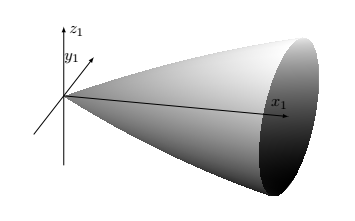
\includegraphics[width=0.9\linewidth]{ParabolicNoseConeAttempt.png}
%\end{subfigure}
\caption{Parabolic cone of constant density $\rho$, frontal thickness $l$, and cone constant $k = 3/4$, corresponding to a three-quarter parabolic nose cone.}
\end{figure}
\noindent
With $k = 0$, all curvature vanishes such that the resulting geometry degenerates into the conical shell, and with $k = 1$, the shape is a true paraboloid such that $\partial_x f(L) = 0$. That is, the cone smoothly matches its curvature for the body on which it will be mounted in the case when $k = 1$. Otherwise, the boundary joining these two components forms an edge.

Introducing nondimensional parameters $\alpha$ and $\ell$ such that $R = \alpha L$ and $l = \ell L$, the properties of the parabolic nose cone are
\begin{gather}
%V = \frac{M}{\rho} = \frac{\pi R^2 L}{3} \left(\frac{20 + 3 (k - 5)k + (20 + 3k(5 + k(\ell - 1)) (\ell - 1)) (\ell - 1)^3}{5(k - 2)^2}\right) \\
\frac{M}{\rho} = \frac{\pi R^2 L}{3} \left(\ell \frac{20(\ell^2 - 3\ell + 3) + 15(\ell^3 - 4\ell^2 + 6\ell - 4)k + 3(\ell^4 - 5\ell^3 + 10\ell^2 - 10\ell + 5)k^2}{5(2 - k)^2}\right) \\
%\overline{x} = \frac{L}{2} \left(\ell \frac{10(\ell^3 - 6\ell + 8) + 6(\ell^4 - 10\ell^2 + 20\ell - 15)k + (\ell^5 - 15\ell^3 + 40\ell^2 -45\ell + 24)k^2}{20 + 3(k - 5)k + (20 + 3k(5 + k(\ell - 1))(\ell - 1))(\ell - 1)^3}\right)
\overline{x} = \frac{L}{2} \left(\frac{10(\ell^3 - 6\ell + 8) + 6(\ell^4 - 10\ell^2 + 20\ell - 15)k + (\ell^5 - 15\ell^3 + 40\ell^2 -45\ell + 24)k^2}{20(\ell^2 - 3\ell + 3) + 15(\ell^3 - 4\ell^2 + 6\ell -4)k + 3(\ell^4 - 5\ell^3 + 10\ell^2 - 10\ell + 5)k^2}\right) \label{eq:StructuresParabolicCOM}
\end{gather}
%The inertia tensor's expression is spared due to length, but indeed may be obtained exactly. It may also be obtained numerically via (\ref{eq:StructuresInertiaTensorOfSegment}) with the direct knowledge of (\ref{eq:StructuresParabolicCOM}) if need be. 
\begin{align}
%I_{xx} &= \frac{MR^2 / 42}{(k - 2)^2 \big(20(\ell^3 - 3\ell^2 + \ell) + 15(\ell^4 - 4\ell^3 + 6\ell^2 - 4\ell)k + 3(\ell^4 - 5\ell^3 + 10\ell^2 - 10\ell + 5)k^2}%1008\big(1 + (\ell - 1)^5\big) - 1680\big(1 - (\ell - 1)^6\big)k + 1080\big(1 + (\ell - 1)^7\big)k^2 - 315\big(1 - (\ell - 1)^8\big)k^3 + 35\big(1 + (\ell - 1)^9\big)k^4
I_{xx} &= \frac{MR^2}{42} \Bigg\{1008\big(1 + (\ell - 1)^5\big) - 1680\big(1 - (\ell - 1)^6\big)k + 1080\big(1 + (\ell - 1)^7\big)k^2 \nonumber \\
&\qquad\qquad - 315\big(1 - (\ell - 1)^8\big)k^3 + 35\big(1 + (\ell - 1)^9\big)k^4\Bigg\} / \Bigg\{(k - 2)^2 \Big(20(\ell^3 - 3\ell^2 + \ell) \nonumber \\
&\qquad\qquad + 15(\ell^4 - 4\ell^3 + 6\ell^2 - 4\ell)k + 3(\ell^4 - 5\ell^3 + 10\ell^2 - 10\ell + 5)k^2 \Big)\Bigg\} \\
I_{yy} &= I_{zz} \\
&= \frac{M L^2}{84}
\Bigg\{
336\Big(2(15 - 10\ell + \ell^4) + 3(5 - 10\ell + 10\ell^2 - 5\ell^3 + \ell^4)\alpha^2\Big) \nonumber \\
&\qquad\qquad - 336\Big((66 - 65\ell + 20\ell^2 + 2\ell^4 - \ell^5) + 5(6 - 15\ell + 20\ell^2 - 15\ell^3 + 6\ell^4 - \ell^5)\alpha^2\Big)k \nonumber \\
&\qquad\qquad +  24\Big((749 - 952\ell + 490\ell^2 - 70\ell^3 + 7\ell^4 - 14\ell^5 + 2\ell^6) \nonumber \\
&\qquad\qquad\qquad\  + 45 (7 - 21\ell + 35\ell^2 - 35\ell^3 + 21\ell^4 - 7\ell^5 + \ell^6)\alpha^2\Big)k^2 \nonumber \\
&\qquad\qquad +   3\Big(-4(532 - 819\ell + 560\ell^2 - 140\ell^3 - 7\ell^5 + 4\ell^6) \nonumber \\
&\qquad\qquad\qquad\  + 105(-8 + 28\ell - 56\ell^2 + 70\ell^3 - 56\ell^4 + 28\ell^5 - 8\ell^6 + \ell^7)\alpha^2\Big)k^3 \nonumber \\
&\qquad\qquad +    \Big(12(70 - 126\ell + 105\ell^2 - 35\ell^3 + \ell^6) \nonumber \\
&\qquad\qquad\qquad\  + 35(9 - 36\ell + 84\ell^2 - 126\ell^3 + 126\ell^4 - 84\ell^5 + 36\ell^6 - 9\ell^7 + \ell^8)\alpha^2\Big)k^4
\Bigg\}
/ \nonumber \\
&\qquad\qquad \Bigg\{
(k-2)^2 \Big(20(\ell^2 - 3\ell + 3) + 15(\ell^3 - 4\ell^2 + 6\ell - 4)k \nonumber \\
&\qquad\qquad\ + 3(\ell^4 - 5\ell^3 + 10\ell^2 - 10\ell+ 5)k^2 \Big)
\Bigg\} %\nonumber \\
%&\qquad\qquad
 - M\overline{x}^2
\end{align}
Notice that taking a double limit as $k \to 0$ (conical shell) and $\ell \to 1$ (solid) correctly yields the desired results of the solid cone. In fact, the limiting results are not particular to the solid cone; they hold for the conical shell too as intended.

Introducing the parabolic nose cone is beneficial in the fact that its results are analytic (specifically, rational functions) and can make use of its freedom with $k$ to closely approximate the structural properties of various others like the tangent and secant ogives, and some of the Haack nose cones, specifically the von K\'{a}rm\'{a}n ogive, whose properties are difficult to obtain/manage exactly.

\subsubsection{Haack Series with Finite Thickness}
The Haack series is summarized here to provide graphical comparison to the parabolic cones. The Haack ogives with \textit{frontal} thickness $0 < l < L$ are obtained by considering $f,g : [0,L] \to \mathbb{R}$ defined by
\begin{align}
f(x; c) = R \sqrt{\frac{1}{\pi}\left(\psi(x) - \frac{\sin 2\psi(x)}{2} + c \sin^3 \psi(x)\right)} && g(x; l) = H(x - l) f(x - l),
\end{align}
where $\psi(x) = \cos^{-1}\big(1 - 2(x/L)\big)$.
The von K\'{a}rm\'{a}n ogive, the nose cone that theoretically sources the least amount of aerodynamic drag, is obtained by setting the cone constant $c = 0$.

\begin{figure}[H]
\centering
\begin{tikzpicture}[scale=2]
% Define the same parameters as above
\pgfmathsetmacro{\m}{0.25}
\pgfmathsetmacro{\L}{3}
\pgfmathsetmacro{\R}{\m*\L}
\pgfmathsetmacro{\K}{0.9}
\pgfmathsetmacro{\t}{0.6} %\R/3

% Draw axes
\draw[->, >=latex, thick] (0,0) -- (2.1,0) node[right]{$x_1$}; %1.5
\draw[->, >=latex, thick] (0,0) -- (0,1.3) node[left]{$y_1$};

%% Draw angle
%\pgfmathsetmacro{\structAngle}{atan(\m)}
%\begin{scope}[shift={(\t,0)}]
%\draw[->, >=stealth, thick] (1, 0) arc(0:\structAngle:1) node[midway, right]{$\theta_c$};
%\end{scope}

% Outside cone
\draw[red, domain=0:\L, samples=120] plot ({\x}, {((\R / (2 - \K)) * (2*\x/\L - \K * (\x/\L)^2)});
\draw[red, domain=0:\L, samples=120] plot ({\x}, {((-\R / (2 - \K)) * (2*\x/\L - \K * (\x/\L)^2)});
% Inside cone
\draw[red, dashed, domain=\t:\L, samples=40] plot ({\x}, {((\R / (2 - \K)) * (2*(\x-\t)/\L - \K * ((\x-\t)/\L)^2)});
\draw[red, dashed, domain=\t:\L, samples=40] plot ({\x}, {((-\R / (2 - \K)) * (2*(\x-\t)/\L - \K * ((\x-\t)/\L)^2)});
% Draw t
\pgfmathsetmacro{\YofLine}{-0.33} %-0.05
\draw[dashed] (0, 0) -- (0, \YofLine);
\draw[dashed] (\t, 0) -- (\t, \YofLine);
\draw[|-|] (0,\YofLine) -- (\t,\YofLine) node[pos=0.5, below]{$l$}; %pos=0.6, below, yshift=-2.3mm

% Draw Haack cone
\pgfmathsetmacro{\c}{0} % von Karman cone
% Outside cone
\draw [domain=0:\L, samples=120] plot ({\x}, {(\R / sqrt(pi)) * sqrt(acos(1 - 2*\x/\L)*pi/180 - sin(2*acos(1 - 2*\x/\L))/2 + \c * sin(acos(1 - 2*\x/\L))^3)});
\draw [domain=0:\L, samples=120] plot ({\x}, {(-\R / sqrt(pi)) * sqrt(acos(1 - 2*\x/\L)*pi/180 - sin(2*acos(1 - 2*\x/\L))/2 + \c * sin(acos(1 - 2*\x/\L))^3)});
% Inside cone
\draw [dashed, domain=\t:\L, samples=40] plot ({\x}, {(\R / sqrt(pi)) * sqrt(acos(1 - 2*(\x-\t)/\L)*pi/180 - sin(2*acos(1 - 2*(\x-\t)/\L))/2 + \c * sin(acos(1 - 2*(\x-\t)/\L))^3)});
\draw [dashed, domain=\t:\L, samples=40] plot ({\x}, {(-\R / sqrt(pi)) * sqrt(acos(1 - 2*(\x-\t)/\L)*pi/180 - sin(2*acos(1 - 2*(\x-\t)/\L))/2 + \c * sin(acos(1 - 2*(\x-\t)/\L))^3)});


%%% Draw vertical thickness
%\pgfmathsetmacro{\XofVerticalMarker}{0.8*\L}
%\pgfmathsetmacro{\YofVerticalMarkerOnInside}{\m*(\XofVerticalMarker-\t)}
%\pgfmathsetmacro{\YofVerticalMarkerOnOutside}{\m*\XofVerticalMarker}
%\pgfmathsetmacro{\tailLength}{0.2}
%\draw[->, >=stealth] (\XofVerticalMarker, -\YofVerticalMarkerOnInside+\tailLength) -- (\XofVerticalMarker, -\YofVerticalMarkerOnInside);
%\draw[->, >=stealth] (\XofVerticalMarker, -\YofVerticalMarkerOnOutside-\tailLength) -- (\XofVerticalMarker, -\YofVerticalMarkerOnOutside) node[left, rotate=-atan(\m), xshift=-1.5mm, yshift=-2.5mm]{$\tan\theta_c \,t$};
%% Draw normal thickness
%\pgfmathsetmacro{\setXOutsideOn}{0.8*\L}
%\pgfmathsetmacro{\setYOutsideOn}{\m*\setXOutsideOn}
%\pgfmathsetmacro{\setXOutsideOff}{\setXOutsideOn-0.05}
%\pgfmathsetmacro{\setYOutsideOff}{\setYOutsideOn -1/\m * (\setXOutsideOff - \setXOutsideOn)}
%%
%\pgfmathsetmacro{\setXInsideOn}{\setXOutsideOn + \m^2*\t/(1+\m^2)}
%\pgfmathsetmacro{\setYInsideOn}{\m*(\setXInsideOn-\t)}
%\pgfmathsetmacro{\setXInsideOff}{\setXInsideOn+0.05}
%\pgfmathsetmacro{\setYInsideOff}{\setYInsideOn -1/\m * (\setXInsideOff - \setXInsideOn)}
%%
%\draw[->, >=stealth] (\setXOutsideOff, \setYOutsideOff) -- (\setXOutsideOn, \setYOutsideOn) node[left, xshift=-2mm, yshift=2mm, rotate=atan(\m)]{$|\sin\theta_c|\tan\theta_c \,t$};
%\draw[->, >=stealth] (\setXInsideOff, \setYInsideOff) -- (\setXInsideOn, \setYInsideOn);

\end{tikzpicture}

%\begin{subfigure}[t]{0.5\textwidth}
%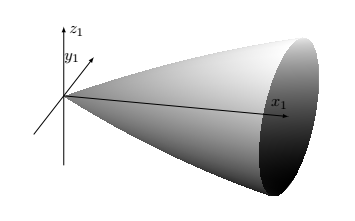
\includegraphics[width=0.9\linewidth]{ParabolicNoseConeAttempt.png}
%\end{subfigure}
\caption{Comparison of the parabolic cone of cone constant $k = 9/10$ (red, slightly inside) and the von K\'{a}rm\'{a}n ogive of the Haack series characterized by the cone constant $c = 0$ (black, slightly outside).}
\end{figure}
\noindent


%Though the properties (mass, center of mass, and inertia tensor) may be obtained exaclty, only the mass (volume) is provided to provide a benchmark; the rest are spared.
%The relevant structural properties are spared except the mass, which is provided to provide a benchmark for validating results when obtaining the exact expressions for the center of mass and inertia tensor.
The mass and center of mass properties are
\begin{align}
V = \frac{M}{\rho} &= \frac{R^2 L}{48} \Big[9c\pi - \left((48 + 18c) - (64 - 12c)\ell + (64 - 144c)\ell^2 + 96c\ell^3\right)\sqrt{(1 - \ell)\ell} \nonumber\\
&\qquad\qquad -6(16\ell + 3c - 8)\cos^{-1}\sqrt{\ell} - 48\sin^{-1}(1 - 2\ell)\Big]
\end{align}

\begin{align}
\overline{x} &= \frac{L}{10}\,\bigg\{(75 + 45c)\pi - \Big((330 + 90 c)  - (590 - 150c)\ell + (660 - 1608c)\ell^2 - (240 - 1944c)\ell^3 \nonumber\\
&\qquad\qquad - (160+384c)\ell^4 - 192c\ell^5\Big)\sqrt{\frac{\ell}{1 - \ell}} - 90c(1 + 2\ell)\cos^{-1}\!\sqrt{\ell} + 15\cos^{-1}(1 - 2\ell) \nonumber\\
%&\qquad\qquad  \nonumber\\
&\qquad\qquad + 240\ell(1 + \ell)\cos^{-1}(2\ell - 1) - 150\sin^{-1}(1-2\ell) \bigg\} / \nonumber \\
&\qquad\quad  \bigg\{(24 + 9c)\pi - \big((48 + 18c) + 12c\ell - 144c\ell^2 + 96c\ell^3\big)\sqrt{(1-\ell)\ell} + 64\sqrt{(1-\ell)\ell}^{\,3} \nonumber \\
&\qquad\qquad + (48 + 96\ell - 18c)\cos^{-1}\sqrt{\ell} - 48\cos^{-1}(2\ell - 1)\bigg\}.
\end{align}
%\begin{align}
%\overline{x} &= \frac{L}{10}\,\bigg\{\!\Big(-(330 + 90 c)  + (590 - 150c)\tau - (660 - 1608c)\tau^2 \nonumber\\
%&\qquad\qquad + (240 - 1944c)\tau^3 + (160+384c)\tau^4 + 192c\tau^5\Big)\sqrt{\frac{\tau}{1 - \tau}} \nonumber\\
%&\qquad\qquad + \pi (75 + 45c) + 15\cos^{-1}(1 - 2\tau) + 240(1 + \tau)\cos^{-1}(2\tau - 1) \nonumber\\
%&\qquad\qquad - 150\sin^{-1}(1-2\tau) - (90c + 180c)\sec^{-1}\!\sqrt{1/\tau}\bigg\} / \nonumber \\
%&\qquad\quad  \bigg\{(24 + 9c)\pi - \big((48 + 18c) + 12c\tau - 144c\tau^2 + 96c\tau^3\big)\sqrt{(1-\tau)\tau} + 64\sqrt{(1-\tau)\tau}^{\,3} \nonumber \\
%&\qquad\qquad - 48\cos^{-1}(2\tau - 1) + (48 + 96\tau - 18c)\sec^{-1}\sqrt{1/\tau}\bigg\}.
%\end{align}
The inertia matrix is spared, but it indeed may be determined from (\ref{eq:StructuresInertiaTensorOfSegment}) exactly or also numerically if need be. Note that the center of mass has a finite limit as $\ell \to 1$. The limit is simply
\begin{equation}
\lim_{\ell \to 1} \overline{x} = L \left(\frac{11 + 3c}{16 + 6c}\right).
\end{equation}

\subsubsection{Elliptical Shell with Finite Thickness}
%It may still be instructive to include the elliptical shell even though no technical results shall be given. 
The elliptical shell with \textit{frontal} thickness $0 < l < L$ may be obtained by considering a new geometry $f, g : [0, L] \to \mathbb{R}$ defined by
\begin{align}
f(x) = R \sqrt{1 - \frac{(x - L)^2}{L^2}} && g(x; l) = H(x - l) f(x - l).
\end{align}
Here, ``new geometry'' means one that does not generalize upon the parabolic nose cone. 
Upon visual inspection of Fig. \ref{fig:StructuresEllipticalCone}, the fundamental difference between the elliptical and the parabolic cones is the tip's sharpness (which has implications as to how shockwaves might behave when experiencing a supersonic flow field). 
Supposing the wall thicknesses are invariant, cones with blunter tips effectively move the center of mass more forward than cones with sharper tips, structurally.
\begin{figure}[H]
\begin{subfigure}[t]{0.5\textwidth}
\centering
\tdplotsetmaincoords{-20}{0} % 70 110
\tdplotsetrotatedcoords{0}{-20}{0}
\begin{tikzpicture}[scale=2, tdplot_main_coords]
\pgfmathsetmacro{\m}{0.25}
\pgfmathsetmacro{\L}{3}
\pgfmathsetmacro{\R}{\m*\L}
\pgfmathsetmacro{\K}{0.75}

% New approach is to draw curve (parabola) on xy plane and rotate plane until it matches well with base
\pgfmathsetmacro{\th}{-20}
\pgfmathsetmacro{\cost}{cos(\th)}
\pgfmathsetmacro{\sint}{sin(\th)}
\begin{scope}[tdplot_rotated_coords, canvas is plane={O(0,0,0)x(1,0,0)y(0,\cost,\sint)}]
\draw [domain=0:\L, samples=40] plot ({\x}, {\R * sqrt(1 - ((\x-\L) / \L)^2)});
\draw [domain=0:\L, samples=40] plot ({\x}, {-\R * sqrt(1 - ((\x-\L) / \L)^2)});
\end{scope}
% Draw face
\begin{scope}[tdplot_rotated_coords, canvas is yz plane at x=\L]
\pgfmathsetmacro{\t}{\R/6}
\draw (0, 0) circle[radius=\R];
\draw (0, 0) circle[radius=\R-\t];
\draw[->, >=stealth, thick] (-\R-0.2,0) -- (-\R,0);
\draw[->, >=stealth, thick] (-\R+\t+0.4,0) -- (-\R+\t,0) node[pos=1.1, right, xshift=1mm]{$R - r$};
\end{scope}
% Draw parameters
\draw[tdplot_rotated_coords, dashed] (0, 0, 0) -- (\L, 0, 0) node[pos=0.6, below]{$L$};
\draw[tdplot_rotated_coords, dashed] (\L, 0, 0) -- (\L, \R, 0) node[above, xshift=-0.5mm, yshift=0.5mm]{$R$};%node[midway, right, xshift=-1mm]{$R$};
%% Draw half angle
%\begin{scope}[tdplot_rotated_coords, canvas is xy plane at z=0]
%\pgfmathsetmacro{\angle}{atan(\R/\L)}
%\draw[->, >=stealth] (1.2,0) arc (0:\angle:1.225cm) node[midway, right]{$\theta_c$};
%\end{scope}

% Draw axes
\draw[->, >=latex, thick, tdplot_rotated_coords] (0, 0, 0) -- (1, 0 ,0) node[anchor=north west, xshift=-2mm]{$x_1$};
\draw[->, >=latex, thick, tdplot_rotated_coords] (0, 0, 0) -- (0, 1 ,0) node[pos=1, right]{$y_1$};
\draw[->, >=latex, thick, tdplot_rotated_coords] (0, 0, 0) -- (0, 0 ,1) node[anchor=north east, xshift=0.75mm, yshift=0.75mm]{$z_1$};
\end{tikzpicture}% NO SPACE!
\end{subfigure}
\hspace{1cm}% NO SPACE!
\begin{subfigure}[t]{0.5\textwidth}
\begin{tikzpicture}[scale=2]
% Define the same parameters as above
\pgfmathsetmacro{\m}{0.25}
\pgfmathsetmacro{\L}{3}
\pgfmathsetmacro{\R}{\m*\L}
\pgfmathsetmacro{\K}{0.75}
\pgfmathsetmacro{\t}{0.6} %\R/3

% Draw axes
\draw[->, >=latex, thick] (0,0) -- (2.1,0) node[right]{$x_1$}; %1.5
\draw[->, >=latex, thick] (0,0) -- (0,1.3) node[left]{$y_1$};

%% Draw angle
%\pgfmathsetmacro{\structAngle}{atan(\m)}
%\begin{scope}[shift={(\t,0)}]
%\draw[->, >=stealth, thick] (1, 0) arc(0:\structAngle:1) node[midway, right]{$\theta_c$};
%\end{scope}

% Outside cone
\draw [domain=0:\L, samples=40] plot ({\x}, {\R * sqrt(1 - ((\x-\L) / \L)^2)});
\draw [domain=0:\L, samples=40] plot ({\x}, {-\R * sqrt(1 - ((\x-\L) / \L)^2)});
% Inside cone
\draw[dashed, domain=\t:\L, samples=40] plot ({\x}, {\R * sqrt(1 - ((\x-\t-\L) / \L)^2) * (1 - sin(180*\t/\L)^2)});
\draw[dashed, domain=\t:\L, samples=40] plot ({\x}, {-\R * sqrt(1 - ((\x-\t-\L) / \L)^2) * (1 - sin(180*\t/\L)^2)});
% Draw t
\pgfmathsetmacro{\YofLine}{-0.65} %-0.05
\draw[dashed] (0, 0) -- (0, \YofLine);
\draw[dashed] (\t, 0) -- (\t, \YofLine);
\draw[|-|] (0,\YofLine) -- (\t,\YofLine) node[pos=0.5, below]{$l$}; %pos=0.6, below, yshift=-2.3mm

%%% Draw vertical thickness
%\pgfmathsetmacro{\XofVerticalMarker}{0.8*\L}
%\pgfmathsetmacro{\YofVerticalMarkerOnInside}{\m*(\XofVerticalMarker-\t)}
%\pgfmathsetmacro{\YofVerticalMarkerOnOutside}{\m*\XofVerticalMarker}
%\pgfmathsetmacro{\tailLength}{0.2}
%\draw[->, >=stealth] (\XofVerticalMarker, -\YofVerticalMarkerOnInside+\tailLength) -- (\XofVerticalMarker, -\YofVerticalMarkerOnInside);
%\draw[->, >=stealth] (\XofVerticalMarker, -\YofVerticalMarkerOnOutside-\tailLength) -- (\XofVerticalMarker, -\YofVerticalMarkerOnOutside) node[left, rotate=-atan(\m), xshift=-1.5mm, yshift=-2.5mm]{$\tan\theta_c \,t$};
%% Draw normal thickness
%\pgfmathsetmacro{\setXOutsideOn}{0.8*\L}
%\pgfmathsetmacro{\setYOutsideOn}{\m*\setXOutsideOn}
%\pgfmathsetmacro{\setXOutsideOff}{\setXOutsideOn-0.05}
%\pgfmathsetmacro{\setYOutsideOff}{\setYOutsideOn -1/\m * (\setXOutsideOff - \setXOutsideOn)}
%%
%\pgfmathsetmacro{\setXInsideOn}{\setXOutsideOn + \m^2*\t/(1+\m^2)}
%\pgfmathsetmacro{\setYInsideOn}{\m*(\setXInsideOn-\t)}
%\pgfmathsetmacro{\setXInsideOff}{\setXInsideOn+0.05}
%\pgfmathsetmacro{\setYInsideOff}{\setYInsideOn -1/\m * (\setXInsideOff - \setXInsideOn)}
%%
%\draw[->, >=stealth] (\setXOutsideOff, \setYOutsideOff) -- (\setXOutsideOn, \setYOutsideOn) node[left, xshift=-2mm, yshift=2mm, rotate=atan(\m)]{$|\sin\theta_c|\tan\theta_c \,t$};
%\draw[->, >=stealth] (\setXInsideOff, \setYInsideOff) -- (\setXInsideOn, \setYInsideOn);

\end{tikzpicture}
\end{subfigure}

%\begin{subfigure}[t]{0.5\textwidth}
%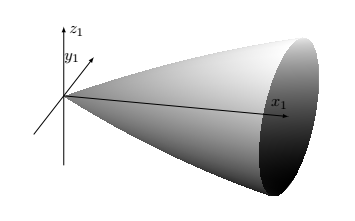
\includegraphics[width=0.9\linewidth]{ParabolicNoseConeAttempt.png}
%\end{subfigure}
\caption{Elliptical cone of constant density $\rho$ and frontal thickness $l$.}
\label{fig:StructuresEllipticalCone}
\end{figure}

The properties of interest follow after defining nondimensional parameters $\alpha = R/L$ and $\ell = l/L$.
\begin{gather}
V = \frac{M}{\rho} = \frac{\pi R^2 L}{3} (\ell^3 - 3\ell), \qquad\quad \overline{x} = \frac{L}{4} \left(\frac{\ell^3 + 4\ell^2 -6\ell - 4}{\ell^2 - 3}\right) \\
[I] = \frac{M L^2}{80} \operatorname{diag}
\renewcommand\arraystretch{2.6}
\begin{pmatrix}
\displaystyle 8 \frac{3\ell^4 - 10\ell^2 + 15}{\ell^2 - 3} \alpha^2 \\
\displaystyle \frac{(3\ell^6 - 44\ell^4 + 80\ell^3 - 60\ell^2 + 40) - 4(3\ell^6 - 19\ell^4 + 45\ell^2 - 45)\alpha^2}{(\ell^2 - 3)^2} \\ 
\displaystyle \frac{(3\ell^6 - 44\ell^4 + 80\ell^3 - 60\ell^2 + 40) - 4(3\ell^6 - 19\ell^4 + 45\ell^2 - 45)\alpha^2}{(\ell^2 - 3)^2}
\end{pmatrix}
\end{gather}

\subsection{Body Configurations} \label{subsec:StructuresBodyConfigs}
\subsubsection{Solid Cylinder}
The solid cylinder is characterized by $f, g: [0, L] \to \mathbb{R}$ defined by
\begin{align}
f(x) = R && g(x) = 0.
\end{align}
With $R$ a fixed constant, the resulting surface described by this geometry is the simplest of all bodies of revolution to analyze.
\begin{figure}[H]
\centering
\tdplotsetmaincoords{-20}{0} % 70 110
\tdplotsetrotatedcoords{0}{-20}{0}
\begin{tikzpicture}[scale=2, tdplot_main_coords]
\pgfmathsetmacro{\m}{0.25}
\pgfmathsetmacro{\L}{3}
\pgfmathsetmacro{\R}{\m*\L}

% Draw sides
\pgfmathsetmacro{\t}{-20}
\pgfmathsetmacro{\Rcost}{\R*cos(\t)}
\pgfmathsetmacro{\Rsint}{\R*sin(\t)}
\draw[tdplot_rotated_coords] (0, \Rcost, \Rsint) -- (\L, \Rcost, \Rsint);
\draw[tdplot_rotated_coords] (0, -\Rcost, -\Rsint) -- (\L, -\Rcost, -\Rsint);
% Draw faces
\begin{scope}[tdplot_rotated_coords, canvas is yz plane at x=0]
\pgfmathsetmacro{\ttmp}{145}
\pgfmathsetmacro{\Rsinttmp}{\R*sin(\ttmp)}
\pgfmathsetmacro{\Rcosttmp}{\R*cos(\ttmp)}
\draw (\Rcost, \Rsint) arc(\t:\ttmp:\R);
\draw[dashed] (\Rcosttmp, \Rsinttmp) arc(\ttmp:360:\R);
\end{scope}
\begin{scope}[tdplot_rotated_coords, canvas is yz plane at x=\L]
\draw (0, 0) circle[radius=\R];
\end{scope}
% Draw parameters
\draw[tdplot_rotated_coords, dashed] (0, 0, 0) -- (\L, 0, 0) node[pos=0.6, below]{$L$};
\draw[tdplot_rotated_coords, dashed] (\L, 0, 0) -- (\L, \R, 0) node[above, xshift=-0.5mm, yshift=0.5mm]{$R$};%node[midway, right, xshift=0mm]{$R$};

% Draw axes
\draw[->, >=latex, thick, tdplot_rotated_coords] (0, 0, 0) -- (1, 0 ,0) node[anchor=north west, xshift=-2mm]{$x_m$};
\draw[->, >=latex, thick, tdplot_rotated_coords] (0, 0, 0) -- (0, 1 ,0) node[pos=1, right]{$y_m$};
\draw[->, >=latex, thick, tdplot_rotated_coords] (0, 0, 0) -- (0, 0 ,1) node[anchor=north east, xshift=0.75mm, yshift=0.75mm]{$z_m$};
\end{tikzpicture}
\caption{Solid cylinder of constant density $\rho$.}
\end{figure}
For constant density $\rho$, the properties (mass, center of mass, and inertia matrix relative to the center of mass) considering the introduction of a nondimensional parameter $\alpha = R/L$ follow
\begin{align}
V = \frac{M}{\rho} = \pi R^2 L, && \overline{x} = \frac{L}{2}, && [I] = \frac{MR^2}{4} \begin{pmatrix}2 & 0 & 0 \\ 0 & 1 & 0 \\ 0 & 0 & 1\end{pmatrix}.
\end{align}


\subsubsection{Hollowed Cylinder}
The hollow cylinder of \textit{inner} radius $0 < r < R$ is characterized by $f, g: [0, L] \to \mathbb{R}$ defined by
\begin{align}
f(x) = R, && g(x) = r.
\end{align}
\begin{figure}[H]
\begin{subfigure}[t]{0.5\textwidth}
\centering
\tdplotsetmaincoords{-20}{0} % 70 110
\tdplotsetrotatedcoords{0}{-20}{0}
\begin{tikzpicture}[scale=2, tdplot_main_coords]
\pgfmathsetmacro{\m}{0.25}
\pgfmathsetmacro{\L}{3}
\pgfmathsetmacro{\R}{\m*\L}

% New approach is to draw curve (parabola) on xy plane and rotate plane until it matches well with base
\pgfmathsetmacro{\th}{-20}
\pgfmathsetmacro{\cost}{cos(\th)}
\pgfmathsetmacro{\sint}{sin(\th)}
\begin{scope}[tdplot_rotated_coords, canvas is plane={O(0,0,0)x(1,0,0)y(0,\cost,\sint)}]
\draw [domain=0:\L, samples=3] plot ({\x}, {\R});
\draw [domain=0:\L, samples=3] plot ({\x}, {-\R});
\end{scope}
% Draw face
\begin{scope}[tdplot_rotated_coords, canvas is yz plane at x=\L]
\pgfmathsetmacro{\t}{\R/6}
\draw (0, 0) circle[radius=\R];
\draw (0, 0) circle[radius=\R-\t];
\draw[->, >=stealth, thick] (-\R-0.2,0) -- (-\R,0);
\draw[->, >=stealth, thick] (-\R+\t+0.4,0) -- (-\R+\t,0) node[pos=1.1, right, xshift=2mm]{$R - r$};
\end{scope}
% Draw faces
%\pgfmathsetmacro{\t}{-20}
\pgfmathsetmacro{\Rcost}{\R*\cost}
\pgfmathsetmacro{\Rsint}{\R*\sint}
\begin{scope}[tdplot_rotated_coords, canvas is yz plane at x=0]
\pgfmathsetmacro{\thtmp}{145}
\pgfmathsetmacro{\Rsinttmp}{\R*sin(\thtmp)}
\pgfmathsetmacro{\Rcosttmp}{\R*cos(\thtmp)}
\draw (\Rcost, \Rsint) arc(\th:\thtmp:\R);
\draw[dashed] (\Rcosttmp, \Rsinttmp) arc(\thtmp:360:\R);
\pgfmathsetmacro{\Rminust}{\R*5/6}
\draw[dashed] (\Rminust, 0) arc(0:360:\Rminust); % Inside face
\end{scope}
% Draw parameters
\draw[tdplot_rotated_coords, dashed] (0, 0, 0) -- (\L, 0, 0) node[pos=0.6, below]{$L$};
\draw[tdplot_rotated_coords, dashed] (\L, 0, 0) -- (\L, \R, 0) node[above, xshift=-0.5mm, yshift=0.5mm]{$R$}; % node[midway, right, xshift=-1mm]{$R$};
%% Draw half angle
%\begin{scope}[tdplot_rotated_coords, canvas is xy plane at z=0]
%\pgfmathsetmacro{\angle}{atan(\R/\L)}
%\draw[->, >=stealth] (1.2,0) arc (0:\angle:1.225cm) node[midway, right]{$\theta_c$};
%\end{scope}

% Draw axes
\draw[->, >=latex, thick, tdplot_rotated_coords] (0, 0, 0) -- (1, 0 ,0) node[anchor=north west, xshift=-2mm]{$x_m$};
\draw[->, >=latex, thick, tdplot_rotated_coords] (0, 0, 0) -- (0, 1 ,0) node[pos=1, right]{$y_m$};
\draw[->, >=latex, thick, tdplot_rotated_coords] (0, 0, 0) -- (0, 0 ,1) node[anchor=north east, xshift=0.75mm, yshift=0.75mm]{$z_m$};
\end{tikzpicture}% NO SPACE!
\end{subfigure}
\hspace{1cm}% NO SPACE!
\begin{subfigure}[t]{0.5\textwidth}
\begin{tikzpicture}[scale=2]
% Define the same parameters as above
\pgfmathsetmacro{\m}{0.25}
\pgfmathsetmacro{\L}{3}
\pgfmathsetmacro{\R}{\m*\L}
\pgfmathsetmacro{\t}{\R/6} %\R/3

% Draw axes
\draw[->, >=latex, thick] (0,0) -- (2.1,0) node[right]{$x_m$}; %1.5
\draw[->, >=latex, thick] (0,0) -- (0,1.3) node[left]{$y_m$};

%% Draw angle
%\pgfmathsetmacro{\structAngle}{atan(\m)}
%\begin{scope}[shift={(\t,0)}]
%\draw[->, >=stealth, thick] (1, 0) arc(0:\structAngle:1) node[midway, right]{$\theta_c$};
%\end{scope}

% Outside cylinder
\draw [domain=0:\L, samples=3] plot ({\x}, {\R});
\draw [domain=0:\L, samples=3] plot ({\x}, {-\R});
% Inside cylinder
\draw[dashed, domain=0:\L, samples=40] plot ({\x}, {\R-\t});
\draw[dashed, domain=0:\L, samples=40] plot ({\x}, {-(\R-\t)});
%% Draw t
%\pgfmathsetmacro{\YofLine}{-0.33} %-0.05
%\draw[dashed] (0, 0) -- (0, \YofLine);
%\draw[dashed] (\t, 0) -- (\t, \YofLine);
%\draw[|-|] (0,\YofLine) -- (\t,\YofLine) node[pos=0.5, below]{$t$}; %pos=0.6, below, yshift=-2.3mm

%% Draw vertical thickness
\pgfmathsetmacro{\XofVerticalMarker}{0.8*\L}
\pgfmathsetmacro{\YofVerticalMarkerOnInside}{\R-\t}
\pgfmathsetmacro{\YofVerticalMarkerOnOutside}{\R}
\pgfmathsetmacro{\tailLength}{0.2}
\draw[->, >=stealth] (\XofVerticalMarker, \YofVerticalMarkerOnInside-\tailLength) -- (\XofVerticalMarker, \YofVerticalMarkerOnInside);
\draw[->, >=stealth] (\XofVerticalMarker, \YofVerticalMarkerOnOutside+\tailLength) -- (\XofVerticalMarker, \YofVerticalMarkerOnOutside) node[right, xshift=0.5mm, yshift=2.25mm]{$R - r$};
%% Draw normal thickness
%\pgfmathsetmacro{\setXOutsideOn}{0.8*\L}
%\pgfmathsetmacro{\setYOutsideOn}{\m*\setXOutsideOn}
%\pgfmathsetmacro{\setXOutsideOff}{\setXOutsideOn-0.05}
%\pgfmathsetmacro{\setYOutsideOff}{\setYOutsideOn -1/\m * (\setXOutsideOff - \setXOutsideOn)}
%%
%\pgfmathsetmacro{\setXInsideOn}{\setXOutsideOn + \m^2*\t/(1+\m^2)}
%\pgfmathsetmacro{\setYInsideOn}{\m*(\setXInsideOn-\t)}
%\pgfmathsetmacro{\setXInsideOff}{\setXInsideOn+0.05}
%\pgfmathsetmacro{\setYInsideOff}{\setYInsideOn -1/\m * (\setXInsideOff - \setXInsideOn)}
%%
%\draw[->, >=stealth] (\setXOutsideOff, \setYOutsideOff) -- (\setXOutsideOn, \setYOutsideOn) node[left, xshift=-2mm, yshift=2mm, rotate=atan(\m)]{$|\sin\theta_c|\tan\theta_c \,t$};
%\draw[->, >=stealth] (\setXInsideOff, \setYInsideOff) -- (\setXInsideOn, \setYInsideOn);

\end{tikzpicture}
\end{subfigure}
\caption{Hollow cylinder of constant density $\rho$ and wall thickness $R - r$.}
\end{figure}
For constant density $\rho$, the properties are
\begin{gather}
V = \frac{M}{\rho} = \pi (R^2 - r^2) L, \qquad\quad \overline{x} = \frac{L}{2}, \label{eq:StructuresHollowCylinderVolumeAndCOM}\\ 
[I] = \frac{M}{12} \operatorname{diag}\begin{pmatrix}6(R^2 + r^2) \\ 3(R^2 + r^2) + L^2 \\ 3(R^2 + r^2) + L^2\end{pmatrix}. \label{eq:StructuresHollowCylinderInertiaTensorwrtCOM}
\end{gather}
Intuitively and indeed, taking $r \to 0$ reduces back to the solid cylinder. Note, however, that taking $r = R$, where the hollow cylinder vanishes, gives nonzero properties.

\subsubsection{Radial Frustum}
The radial frustum is obtained by cutting a circular cone with two vertical planes at $x = a$ and $x = b$ with $0 < a < b$, where then the length of the frustum is $L = b - a$. The form of $f, g$ may therefore be borrowed from the case of the conical shell (Fig. \ref{fig:StructuresConicalShell}) by applying a remapping $x \mapsto x - a$, effecting functions $f, g : [0,L] \to \mathbb{R}$ of the form 
\begin{align}
f(x) = R_0 + \frac{R - R_0}{L} x && g(x) = f(x - l),
\end{align}
where $R_0$ is the outer radius at $x = 0$, $R$ is the outer radius at $x = L$, and $0 < l < R_0 L / (R_0 + R)$ is the \textit{frontal} thickness. 
\begin{figure}[H]
\begin{subfigure}[t]{0.5\textwidth}
\centering
\tdplotsetmaincoords{-20}{0} % 70 110
\tdplotsetrotatedcoords{0}{-20}{0}
\begin{tikzpicture}[scale=2, tdplot_main_coords]
\pgfmathsetmacro{\m}{0.25}
\pgfmathsetmacro{\L}{3}
\pgfmathsetmacro{\r}{\m*\L*0.8}
\pgfmathsetmacro{\R}{1.6*\r}

% New approach is to draw curve (parabola) on xy plane and rotate plane until it matches well with base
\pgfmathsetmacro{\th}{-20}
\pgfmathsetmacro{\cost}{cos(\th)}
\pgfmathsetmacro{\sint}{sin(\th)}
\begin{scope}[tdplot_rotated_coords, canvas is plane={O(0,0,0)x(1,0,0)y(0,\cost,\sint)}]
\draw [domain=0:\L, samples=3] plot ({\x}, {\r + ((\R - \r)/\L)*\x});
\draw [domain=0:\L, samples=3] plot ({\x}, {-(\r + ((\R - \r)/\L)*\x)});
\end{scope}
% Draw face
\pgfmathsetmacro{\t}{\R/6} %R/6
\begin{scope}[tdplot_rotated_coords, canvas is yz plane at x=\L]
\draw (0, 0) circle[radius=\R];
\draw (0, 0) circle[radius=\R-\t];
\draw[->, >=stealth, thick] (-\R-0.2,0) -- (-\R,0);
\draw[->, >=stealth, thick] (-\R+\t+0.4,0) -- (-\R+\t,0) node[pos=1.1, right, xshift=2mm]{$R - r$};
\end{scope}
% Draw faces
%\pgfmathsetmacro{\t}{-20}
\pgfmathsetmacro{\Rcost}{\R*\cost}
\pgfmathsetmacro{\Rsint}{\R*\sint}
\begin{scope}[tdplot_rotated_coords, canvas is yz plane at x=0]
\pgfmathsetmacro{\thtmp}{145}
\pgfmathsetmacro{\Rsinttmp}{\r*sin(\thtmp)}
\pgfmathsetmacro{\Rcosttmp}{\r*cos(\thtmp)}
\pgfmathsetmacro{\Rsinttmpforr}{\r*sin(-180)}
\pgfmathsetmacro{\Rcosttmpforr}{\r*cos(-180)}
\draw[dashed] (0,0) -- (\Rcosttmpforr, \Rsinttmpforr) node[below, yshift=-1mm]{$R_0$};
\draw (\r*\cost, \r*\sint) arc(\th:\thtmp:\r);
\draw[dashed] (\Rcosttmp, \Rsinttmp) arc(\thtmp:360:\r);
\pgfmathsetmacro{\Rminust}{\r-\t}
\draw[dashed] (\Rminust, 0) arc(0:360:\Rminust); % Inside face
\end{scope}
%\begin{scope}[tdplot_rotated_coords, canvas is yz plane at x=\L]
%\draw (0, 0) circle[radius=\R];
%\end{scope}
% Draw parameters
\draw[tdplot_rotated_coords, dashed] (0, 0, 0) -- (\L, 0, 0) node[pos=0.6, below]{$L$};
\draw[tdplot_rotated_coords, dashed] (\L, 0, 0) -- (\L, \R, 0) node[above, xshift=-0.5mm, yshift=0.5mm]{$R$};%node[midway, right, xshift=-1mm]{$R_L$};
%% Draw half angle
%\begin{scope}[tdplot_rotated_coords, canvas is xy plane at z=0]
%\pgfmathsetmacro{\angle}{atan(\R/\L)}
%\draw[->, >=stealth] (1.2,0) arc (0:\angle:1.225cm) node[midway, right]{$\theta_c$};
%\end{scope}

% Draw axes
\draw[->, >=latex, thick, tdplot_rotated_coords] (0, 0, 0) -- (1, 0 ,0) node[anchor=north west, xshift=-2mm]{$x_m$};
\draw[->, >=latex, thick, tdplot_rotated_coords] (0, 0, 0) -- (0, 1 ,0) node[pos=1, right]{$y_m$};
\draw[->, >=latex, thick, tdplot_rotated_coords] (0, 0, 0) -- (0, 0 ,1) node[anchor=north east, xshift=0.75mm, yshift=0.75mm]{$z_m$};
\end{tikzpicture}% NO SPACE!
\end{subfigure}
\hspace{1cm}% NO SPACE!
\begin{subfigure}[t]{0.5\textwidth}
\begin{tikzpicture}[scale=2]
% Define the same parameters as above
\pgfmathsetmacro{\m}{0.25}
\pgfmathsetmacro{\L}{3}
\pgfmathsetmacro{\r}{\m*\L*0.8}
\pgfmathsetmacro{\R}{1.6*\r}
\pgfmathsetmacro{\t}{\R/6} %\R/3

% Draw axes
\draw[->, >=latex, thick] (0,0) -- (2.1,0) node[right]{$x_m$}; %1.5
\draw[->, >=latex, thick] (0,0) -- (0,1.3) node[left]{$y_m$};

%% Draw angle
%\pgfmathsetmacro{\structAngle}{atan(\m)}
%\begin{scope}[shift={(\t,0)}]
%\draw[->, >=stealth, thick] (1, 0) arc(0:\structAngle:1) node[midway, right]{$\theta_c$};
%\end{scope}

% Outside cylinder
\draw [domain=0:\L, samples=3] plot ({\x}, {\r + ((\R - \r)/\L)*\x});
\draw [domain=0:\L, samples=3] plot ({\x}, {-(\r + ((\R - \r)/\L)*\x)});
% Inside cylinder
\draw[dashed, domain=0:\L, samples=40] plot ({\x}, {\r-\t + ((\R - \r)/\L)*(\x)});
\draw[dashed, domain=0:\L, samples=40] plot ({\x}, {-(\r-\t + ((\R - \r)/\L)*(\x))});
%% Draw t
%\pgfmathsetmacro{\YofLine}{-0.33} %-0.05
%\draw[dashed] (0, 0) -- (0, \YofLine);
%\draw[dashed] (\t, 0) -- (\t, \YofLine);
%\draw[|-|] (0,\YofLine) -- (\t,\YofLine) node[pos=0.5, below]{$t$}; %pos=0.6, below, yshift=-2.3mm

% Draw vertical thickness
\pgfmathsetmacro{\XofVerticalMarker}{0.8*\L}
\pgfmathsetmacro{\YofVerticalMarkerOnInside}{-(\r+(\R-\r)/\L*\XofVerticalMarker)}
\pgfmathsetmacro{\YofVerticalMarkerOnOutside}{-(\r-\t+(\R-\r)/\L*\XofVerticalMarker)}
\pgfmathsetmacro{\tailLength}{0.2}
\pgfmathsetmacro{\slope}{(\R - \r)/\L}
\draw[->, >=stealth] (\XofVerticalMarker, \YofVerticalMarkerOnInside-\tailLength) -- (\XofVerticalMarker, \YofVerticalMarkerOnInside) node[pos=0,left, rotate=-atan(\slope), xshift=-1.5mm, yshift=1mm]{$\tan\theta_c \,l$};
\draw[->, >=stealth] (\XofVerticalMarker, \YofVerticalMarkerOnOutside+\tailLength) -- (\XofVerticalMarker, \YofVerticalMarkerOnOutside);%node[right, xshift=1.5mm, yshift=2.5mm]{$t$};
% Draw normal thickness
\pgfmathsetmacro{\setXOutsideOn}{0.8*\L}
\pgfmathsetmacro{\setYOutsideOn}{\r + (\R - \r)/\L*\setXOutsideOn}
\pgfmathsetmacro{\setXOutsideOff}{\setXOutsideOn-0.05}
\pgfmathsetmacro{\setYOutsideOff}{\setYOutsideOn -1/\slope * (\setXOutsideOff - \setXOutsideOn)}
%
\pgfmathsetmacro{\anglef}{atan(\slope)}
\pgfmathsetmacro{\setXInsideOn}{\setXOutsideOn + \t*sin(\anglef)*cos(\anglef)}%\slope^2*\t/(1+\slope^2)}
\pgfmathsetmacro{\setYInsideOn}{-3.9*\t+(\r-\t + (\R - \r)/\L)*(\setXInsideOn)}
\pgfmathsetmacro{\setXInsideOff}{\setXInsideOn+0.05}
\pgfmathsetmacro{\setYInsideOff}{\setYInsideOn -1/\slope * (\setXInsideOff - \setXInsideOn)}
%
\draw[->, >=stealth] (\setXOutsideOff, \setYOutsideOff) -- (\setXOutsideOn, \setYOutsideOn) node[left, xshift=-2mm, yshift=2mm, rotate=atan(\slope)]{$\sin\theta_c\tan\theta_c \,l$};
\draw[->, >=stealth] (\setXInsideOff, \setYInsideOff) -- (\setXInsideOn, \setYInsideOn);

% Draw cone angle on x axis
%\pgfmathsetmacro{\xOffset}{\L * \r / (\r + \R)}
\draw[->, >=stealth, thick] (1, 0) arc(0:atan(\slope):4.6) node[midway,right]{$\theta_c$};

\end{tikzpicture}
\end{subfigure}
\caption{Hollow conical frustum of constant density $\rho$ and wall thickness $l$.}
\label{fig:StructuresHollowFrustum}
\end{figure}
The properties of the frustum of constant density and nondimensional parameters $\alpha = R/L$, $\beta = R_0 / L$, and $\ell = l/L$ follow.
%\begin{gather}
% Same as form below but written "better"
%V = \frac{M}{\rho} = \pi L^3 \big((\alpha - \beta)(\alpha + \beta - (\alpha - \beta)\ell\big)\ell, \qquad\quad \overline{x} = \frac{L}{6}\left(\frac{\alpha (4 - 3\ell) + \beta (2 + 3\ell)}{\alpha + \beta - (\alpha - \beta)\ell}\right)
%\end{gather}
\begin{gather}
V = \frac{M}{\rho} = \pi L^3 \big((\alpha^2 - \beta^2)\ell - (\alpha - \beta)^2\ell^2\big), \qquad\quad \overline{x} = \frac{L}{6}\left(\frac{4\alpha + 2\beta - 3(\alpha - \beta)\ell}{\alpha + \beta - (\alpha - \beta)\ell}\right) % numerator: \alpha (4 - 3\ell) + \beta (2 + 3\ell)
\end{gather}
\begin{align}
%I_{xx} &= \frac{M L^2}{2} \big(\alpha^2(1 -\ell + \ell^2) - 2\alpha\beta\ell^2 + \beta^2 (1 + \ell + \ell^2)\big) \\
I_{xx} &= \frac{M L^2}{2} \big(\alpha^2 + \beta^2 - (\alpha^2 - \beta^2) \ell + (\alpha - \beta)^2 \ell^2\big) \\
I_{yy} &= I_{zz} \\\
&= \frac{M L^2}{36} \frac{1}{(\alpha + \beta - (\alpha - \beta)\ell)^2}\Big\{(2\alpha^2 + 9\alpha^4 + 8\alpha\beta + 18\alpha^3\beta + 2\beta^2 + 18\alpha^2\beta^2 + 18\alpha\beta^3 + 9\beta^4) \nonumber \\
&\qquad\qquad - 3(\alpha^2 + 9\alpha^4 + 6\alpha^3\beta - 2\beta^2 - 6\alpha\beta^3 - 9\beta^4)\ell \nonumber \\
&\qquad\qquad + 3(\alpha^2 + 12\alpha^4 - 2\alpha\beta - 6\alpha^3\beta + \beta^2 - 12\alpha^2\beta^2 + 12\beta^4)\ell^2 \nonumber \\
&\qquad\qquad - 27(\alpha^4 - 2\alpha^3\beta + 2\alpha\beta^3 - \beta^4)\ell^3 \nonumber \\
&\qquad\qquad + 9(\alpha^4 - 4\alpha^3\beta + 6\alpha^2\beta^2 - 4\alpha\beta^3 + \beta^4)\ell^4\Big\}.
\end{align}
Note that under this construction, taking $\beta \to \alpha$ yields $R_0 \to R$ and thus $\theta_c \to 0$, which reduces the above results to those of the cylindrical sheet (of zero thickness).

If the frustum is of the form $R_0 > R$, then the above results hold as viewed from the frame opposite of the current frame with its $x$ and $y$ axes reversed (so that it appears to copy the form of Fig. \ref{fig:StructuresHollowFrustum}). As such, the results hold in this case under the transformation $x \mapsto L - x$; no transformation is necessary to correct results on the $y$ axis since the opposing frame is still radially symmetric about the $x$ axis.




\subsection{Cavity Tuning}
The inside surface of each geometry characterized by the function $g(x; l) = H(x - l)f(x - l)$ can be further generalized by considering a remapping of the surface $g(x; l)$ as
\begin{equation}
g(x; l) \mapsto H(x - l) f(x - l) h(l). \label{eq:StructuresGeneralizedG}
\end{equation}
Specifically, the previously considered nose cones were special cases of (\ref{eq:StructuresGeneralizedG}) such that $h(l) \equiv 1$. As $l$ is simply a parameter of the geometry, $h(l)$ poses no trouble for the procedure of integration; it simply appears repeatedly throughout the results. When choosing $h$, the bound
\begin{equation}
f(x - l)h(l) < f(x)
\end{equation}
should be respected to ensure physical nose cones or other geometries are realized.

\chapter{Propulsion}
Most air and space vehicles (jets, rockets, spacecraft, etc.) utilize some sort of propulsive device to change their current state by ejecting mass out from their systems. That is, the effect of propulsion is to deliver a reactionary force imparted by a fluid particle leaving the system in which it was carried. This idea is realized by the conservation of momentum for a system of initial mass $m + dm$, where the mass of the fluid particle is $dm$, travelling at a velocity $\vec{v}$ .
\begin{equation}
(m + dm) \vec{v} = m (\vec{v} + d\vec{v}) + dm (\vec{v} - \vec{v}_e).
\end{equation}
Here, $\vec{v}_e$ is the exit velocity of the fluid particle relative to the system (as if the system was stationary).
%\end{align}
Consequently, the force is written
\begin{equation}
\vec{F} = \frac{dm}{dt} \vec{v}_e,
\end{equation}
where $m$ identifies the current mass of the system. Inherently then, this rate $\dot{m}$ is always nonpositive during free flight. This negativity, however, is again negated by the fact that $\vec{v}_e$ acts in the direction opposite to the system's velocity $\vec{v}$. Thus, the resulting force on the system acts in the direction of its velocity $\vec{v}$. This force, however, is \textit{not} the force of thrust. A closer inspection reveals that the conservation of momentum in this context is actually realized by
\begin{equation}
\vec{F}_T - \iint_S p \hat{n} \, dS = \frac{\partial}{\partial t} \iiint_V \rho \vec{v} \,dV + \iint_S \rho \vec{v} \,(\vec{v} \cdot \hat{n}) \,dS, \label{eq:PropulsionMomentumEq}
\end{equation}
where $\vec{F}_T$ is the force of thrust, $p$ and $\rho$ are static air pressure and static air density, and $\hat{n}$ is the unit outward normal to the control volume of surface area $S$ and volume $V$. An assumption that the exit velocity is constant and completely perpendicular to the plane spanning across the nozzle's exit, which is decent, yields from (\ref{eq:PropulsionMomentumEq}) that
\begin{equation}
\vec{F}_T \approx \big(\dot{m} v_e + (p_e - p_n) A_e\big) \hat{v}. \label{eq:PropulsionThrustAppx}
\end{equation}
Here, the subscripts $n$ and $e$ respectively denote positions at the vehicle's nose tip and nozzle exit. When moving at supersonic speed with a sharp nose tip, this pressure becomes the freestream pressure $p_\infty$ since, by definition of being supersonic, perturbations cannot propagate their way upstream to influence incoming fluid properties. Otherwise, a blunt-nosed body creates a bow shock, which induces complicatations in finding the air pressure acting on the nose.
\begin{figure}[H]
\centering
\begin{tikzpicture}
%% Temporary axis (comment out this bit when done)
%\draw[red] (0,0) -- (1,0);
%\draw[red] (0,0) -- (0,1);

% Draw the nozzle
\begin{axis}[width=15cm,
			height=207pt,
			at={(-6.71cm,0pt)},
			xmin=-8.5, xmax=1.5,
			ymin=-15, ymax=10,
			hide axis,
			]
%% Temporary axis (comment out this bit when done)
%\draw[blue] (0,0) -- (1,0);
%\draw[blue] (0,0) -- (0,1);
% Plot the diverging section - must keep curves as trig forms for constants to work (1 is hardcoded)
\pgfmathsetmacro{\YOfNozzleThroat}{1} % 1
\pgfmathsetmacro{\YOfNozzleExit}{2} % 3
\pgfmathsetmacro{\A}{(\YOfNozzleThroat + \YOfNozzleExit) / 2}
\pgfmathsetmacro{\B}{(\YOfNozzleThroat - \YOfNozzleExit) / 2}
\addplot[domain=0:1, samples=100, smooth, solid]{\A + \B * cos(deg(pi*x))};
\addplot[domain=0:1, samples=100, smooth, solid]{-\A - \B * cos(deg(pi*x))};
% Plot the converging part
\pgfmathsetmacro{\XOfBodyNozzleIntersection}{-0.25} % -0.25
\pgfmathsetmacro{\YOfBody}{1.5} % 1.25
\pgfmathsetmacro{\C}{(\YOfNozzleThroat + \YOfBody) / 2}
\pgfmathsetmacro{\D}{(\YOfNozzleThroat - \YOfBody) / 2}
\pgfmathsetmacro{\E}{1/\XOfBodyNozzleIntersection}
\addplot[domain=\XOfBodyNozzleIntersection:0, samples=100, smooth, solid]{\C + \D * cos(deg(\E*pi*x))};
\addplot[domain=\XOfBodyNozzleIntersection:0, samples=100, smooth, solid]{-\C - \D * cos(deg(\E*pi*x))};
% Plot the body
\pgfmathsetmacro{\XofConeBodyIntersection}{-6}
\addplot[domain=\XofConeBodyIntersection:\XOfBodyNozzleIntersection, samples=100, smooth, solid]{\YOfBody};
\addplot[domain=\XofConeBodyIntersection:\XOfBodyNozzleIntersection, samples=100, smooth, solid]{-\YOfBody};
% Plot the nose as half of an ellipse
\pgfmathsetmacro{\a}{2}
\pgfmathsetmacro{\b}{\YOfBody}
\pgfmathsetmacro{\XofNoseTip}{\XofConeBodyIntersection-\a}
\addplot[domain=\XofNoseTip:\XofConeBodyIntersection, samples=100, smooth, solid]{\b * sqrt(1 - (x - \XofConeBodyIntersection)^2 / \a^2};
\addplot[domain=\XofNoseTip:\XofConeBodyIntersection, samples=100, smooth, solid]{-\b * sqrt(1 - (x - \XofConeBodyIntersection)^2 / \a^2};

% Place an ellipse on the nozzle to show that it's open ***(only shows if axis is hidden)***
\draw (1,-\YOfNozzleExit) arc (-90:90:1.5pt and 13pt);
\draw[dashed] (1, \YOfNozzleExit) arc (90:270:1.5pt and 13pt);

%% Draw a "cutaway" to show the fuel and chamber inside
\pgfmathsetmacro{\XOfFuel}{-5}
\pgfmathsetmacro{\XOfChamberOffsetFromNozzleTubeIntersection}{0.3}
\pgfmathsetmacro{\XOfChamber}{\XOfBodyNozzleIntersection-\XOfChamberOffsetFromNozzleTubeIntersection}
\pgfmathsetmacro{\YOffsetFromWall}{0.3}
\draw[fill=red!80!black!30] (\XOfFuel,\YOfBody) arc (90:-90:0.6pt and 8.7pt) -- (\XOfChamber, -\YOfBody+\YOffsetFromWall) arc (-90:90:1.2pt and 8.7pt) -- (\XOfFuel,\YOfBody) node[midway, above]{fuel};
\draw[fill=red!80!black!60] (\XOfChamber, \YOfBody) arc (90:-90:1.2pt and 8.7pt) -- (\XOfBodyNozzleIntersection, -\YOfBody+\YOffsetFromWall) arc (-90:90:1.4pt and 8.7pt) -- (\XOfChamber, \YOfBody) node[midway, above]{chamber};

% Draw an axis at the bottom to display various points along the rocket (n, t, e)
\pgfmathsetmacro{\YOfXLine}{-\YOfBody-1.6}
\pgfmathsetmacro{\tickHeight}{1}
\pgfmathsetmacro{\XOfChamberTick}{\XOfChamber + 0.16}
\draw (\XofNoseTip, \YOfXLine) -- (1, \YOfXLine);
\draw (\XofNoseTip, \YOfXLine-\tickHeight/2) -- (\XofConeBodyIntersection-\a, \YOfXLine+\tickHeight/2) node[below, yshift=-2.65mm]{$n$}; % yshift=-2.6mm
\draw (0, \YOfXLine-\tickHeight/2) -- (0, \YOfXLine+\tickHeight/2) node[below, yshift=-2mm]{$t$}; % yshift=-2mm
\draw (\XOfChamberTick, \YOfXLine-\tickHeight/2) -- (\XOfChamberTick, \YOfXLine+\tickHeight/2) node[below, yshift=-2.65mm]{$c$}; % yshift=-2.75mm
\draw (1, \YOfXLine-\tickHeight/2) -- (1, \YOfXLine+\tickHeight/2) node[below, yshift=-2.65mm]{$e$}; % yshift=-2.75mm

% Draw pressures
\draw[->, >=latex] (\XofNoseTip-1.5, 0) -- (\XofNoseTip, 0);% node[above, xshift=-4mm]{$p_n$};
\draw[->, >=latex] (2.5, \YOfNozzleExit) -- (1, \YOfNozzleExit);
\draw[->, >=latex] (2.5, \YOfNozzleExit/2) -- (1, \YOfNozzleExit/2);
\draw[->, >=latex] (2.5, 0) -- (1, 0);% node[above, xshift=4mm]{$p_e$};
\draw[->, >=latex] (2.5, -\YOfNozzleExit) -- (1, -\YOfNozzleExit);
\draw[->, >=latex] (2.5, -\YOfNozzleExit/2) -- (1, -\YOfNozzleExit/2);

% Draw mass flow rate
\draw[->, >=latex, dashed] (0,0) -- (0.4, 0) node[right]{$\dot{m}$};

%% Draw shock
%% Commented this out since it really concerns aerodynamics
%\addplot[domain=\XofNoseTip-0.05:\XofNoseTip+1, samples=250, smooth, solid]{sqrt(1 - (x - (\XofConeBodyIntersection-0.05))^2 / \a^2) * (\b+1.6)};

% Draw center of mass for v and F
\pgfmathsetmacro{\xcom}{-2.6}
\pgfmathsetmacro{\ycom}{0}
\pgfmathsetmacro{\rcom}{\YOfBody/4}
\draw (\xcom, \ycom) node[circle, fill, inner sep=1]{};
\draw[->, >=latex] (\xcom, \ycom) -- (\xcom-0.4, \ycom) node[left]{$\hat{v}$};
%\draw[->, >=latex] (\xcom+0.6, \ycom) -- (\xcom, \ycom) node[pos=0,right]{$\vec{F}_T$};
\end{axis}

% Try to draw center of mass
\begin{scope}[shift={(1.2,2.415)}] % (1.2, 2.4225)
\pgfmathsetmacro{\Bx}{0}
\pgfmathsetmacro{\By}{1}
\pgfmathsetmacro{\Br}{0.11}
\draw[fill=black] (\Bx,\By) ++(0:\Br)   arc (0:90:\Br)    -- (\Bx,\By) -- cycle;
\draw[fill=white] (\Bx,\By) ++(90:\Br)  arc (90:180:\Br)  -- (\Bx,\By) -- cycle;
\draw[fill=black] (\Bx,\By) ++(180:\Br) arc (180:270:\Br) -- (\Bx,\By) -- cycle;
\draw[fill=white] (\Bx,\By) ++(270:\Br) arc (270:360:\Br) -- (\Bx,\By) -- cycle;
\end{scope}

% Draw pressure on nose and exit
\node at (7,3.4){$p_e$};
\node at (-7,3.4){$p_n$};
    % more arrows here
\end{tikzpicture}
\caption{Overviewing diagram of the systems and quantities relevant to the basics of rocket propulsion. Particularly, this diagram contains no aerodynamic considerations (shockwaves) in the visualization of $p_n$ nor in the exhaust field. The fuel is represented by a block-cutaway to reserve space for either solid propellant or liquid fuel and oxidizer. The chamber, leading into the nozzle, is characterized by a constant total pressure, total temperature, and total density. The exhaust velocity is not shown since its reference frame (the rocket) is different from the reference frame monitoring the velocity and thrust force. The exit area $A_e$ is simply the cross-sectional area of the nozzle at the exit.}
\label{fig:PropFuelRocket}
\end{figure}

\section{Quasi-Unidimensional Nozzle Flow}
Gas expelled from a system is typically done so by sourcing a large chamber pressure, typically denoted $p_c$, (which is a total pressure) to force the gas through a \textit{nozzle} which produces an exit pressure $p_e$ along nozzle's exit plane among many other things. Thus, gas flow within a rotationally symmetric geometry is of interest to determine the amount of thrust produced.

The \textit{de Laval} nozzle, or simply called the \textit{converging-diverging} nozzle, is characterized by a symmetrically converging section in which all gas flow is subsonic, a \textit{throat}, and a diverging section in which the gas flow may be subsonic, supersonic, or a combination of both.

The throat is the critical region that determines the flow field in the diverging section of the nozzle. A true fact is that the flow here can be only sonic (Mach 1) \textit{at most}. Thus, a flow that is subsonic at the throat is necessarily subsonic in the diverging section, so the flow is entirely subsonic. A flow, however, that is sonic at the throat and has sufficient chamber pressure $p_c$ relative to the backpressure, denoted $p_b$, to push the flow into the supersonic regime will be supersonic in the diverging section and will continue to be so unless encountering a shockwave in the section.
%, which is the location of the nozzle's minimum cross-sectional area and where supersonic flow \textit{always} begins to choke. Thus, the Mach number at the throat is always unity in a flow exceeding the speed of sound anywhere within the nozzle. If supplied a completely subsonic flow, however, then the Mach number at the throat is less than unity of course, and the rest of the flow to follow the throat is therefore determined to be subsonic. The throat leads into the \textit{diverging} section of the nozzle where \textit{supersonic} flow can occur.
%
The flow regime of the nozzle is largely determined by the pressure ratio $p_b / p_c$ of the back pressure to the chamber pressure and the area ratio $A_e / A_t$ of the exit area to the throat area.

Because the de Laval nozzle is diverging past the throat by definition, then a safe assumption is that the area $A$ is monotonically increasing past the throat. Consequently, the nondimensional stations $x$ along the nozzle's longitudinal axis, where $x = 0$ indicates the throat and $x = 1$ indicates the nozzle exit, are obtainable through the areas via
\begin{equation}
x = \frac{A - A_t}{A_e - A_t}. \label{eq:nondimPosNozzle}
\end{equation}
This nondimensional distance therefore interprets physical locations within the nozzle as a percentage downstream of the throat up until the exit.
\begin{figure}[H]
\centering
\begin{tikzpicture}
%% Temporary axis (comment out this bit when done)
%\draw[red] (0,0) -- (1,0);
%\draw[red] (0,0) -- (0,1);

% Draw the nozzle
\begin{axis}[width=15cm,
			height=207pt,
			at={(-6.71cm,0pt)},
			xmin=-1.05, xmax=1.5,
			ymin=-5, ymax=5,
			hide axis,
			]
%% Temporary axis (comment out this bit when done)
%\draw[blue] (0,0) -- (1,0);
%\draw[blue] (0,0) -- (0,1);
% Plot the diverging section - must keep curves as trig forms for constants to work (1 is hardcoded)
\pgfmathsetmacro{\YOfNozzleThroat}{1} % 1
\pgfmathsetmacro{\YOfNozzleExit}{3} % 3 | 2 | 2.5
\pgfmathsetmacro{\A}{(\YOfNozzleThroat + \YOfNozzleExit) / 2}
\pgfmathsetmacro{\B}{(\YOfNozzleThroat - \YOfNozzleExit) / 2}
\addplot[domain=0:1, samples=100, smooth, solid]{\A + \B * cos(deg(pi*x))};
\addplot[domain=0:1, samples=100, smooth, solid]{-\A - \B * cos(deg(pi*x))};
% Plot the converging part
\pgfmathsetmacro{\XOfBodyNozzleIntersection}{-0.25} % -0.25
\pgfmathsetmacro{\YOfBody}{1.5} % 1.25
\pgfmathsetmacro{\C}{(\YOfNozzleThroat + \YOfBody) / 2}
\pgfmathsetmacro{\D}{(\YOfNozzleThroat - \YOfBody) / 2}
\pgfmathsetmacro{\E}{1/\XOfBodyNozzleIntersection}
\addplot[domain=\XOfBodyNozzleIntersection:0, samples=100, smooth, solid]{\C + \D * cos(deg(\E*pi*x))};
\addplot[domain=\XOfBodyNozzleIntersection:0, samples=100, smooth, solid]{-\C - \D * cos(deg(\E*pi*x))};
% Plot the chamber
\pgfmathsetmacro{\XOfFuel}{-5}
\pgfmathsetmacro{\XOfChamberOffsetFromNozzleTubeIntersection}{0}
\pgfmathsetmacro{\XOfChamber}{\XOfBodyNozzleIntersection-\XOfChamberOffsetFromNozzleTubeIntersection}
\pgfmathsetmacro{\YOffsetFromWall}{0.3}
\pgfmathsetmacro{\XofConeBodyIntersection}{-0.4}
\addplot[domain=\XofConeBodyIntersection:\XOfBodyNozzleIntersection, samples=100, smooth, solid]{\YOfBody};
\addplot[domain=\XofConeBodyIntersection:\XOfBodyNozzleIntersection, samples=100, smooth, solid]{-\YOfBody};
% Plot the nose as half of an ellipse
\pgfmathsetmacro{\a}{2}
\pgfmathsetmacro{\b}{\YOfBody}
%\pgfmathsetmacro{\XofNoseTip}{\XofConeBodyIntersection-\a}
%\addplot[domain=\XofNoseTip:\XofConeBodyIntersection, samples=100, smooth, solid]{\b * sqrt(1 - (x - \XofConeBodyIntersection)^2 / \a^2};
%\addplot[domain=\XofNoseTip:\XofConeBodyIntersection, samples=100, smooth, solid]{-\b * sqrt(1 - (x - \XofConeBodyIntersection)^2 / \a^2};

% Place an ellipse on the nozzle to show that it's open ***(only shows if axis is hidden)***
\draw (1,-\YOfNozzleExit) arc (-90:90:1.5pt and 48.5pt);
\draw[dashed] (1, \YOfNozzleExit) arc (90:270:1.5pt and 48.5pt);

% Place an ellipse on the throat to show that it's open
\draw[dashed] (0,-\YOfNozzleThroat) arc (-90:90:1.5pt and 16pt);
\draw (0, \YOfNozzleThroat) arc (90:270:1.5pt and 16pt);


%% Draw a "cutaway" to show the fuel and chamber inside
%\draw[fill=red!80!black!30] (\XOfFuel,\YOfBody) arc (90:-90:0.6pt and 8.7pt) -- (\XOfChamber, -\YOfBody+\YOffsetFromWall) arc (-90:90:1.2pt and 8.7pt) -- (\XOfFuel,\YOfBody) node[midway, above]{fuel};
%\draw[fill=red!80!black!60] (\XOfChamber, \YOfBody) arc (90:-90:1.2pt and 8.7pt) -- (\XOfBodyNozzleIntersection, -\YOfBody+\YOffsetFromWall) arc (-90:90:1.4pt and 8.7pt) -- (\XOfChamber, \YOfBody) node[midway, above]{chamber};

% Draw an axis at the bottom to display various points along the rocket (n, t, e)
\pgfmathsetmacro{\YOfXLine}{-\YOfBody-1.6-1}
\pgfmathsetmacro{\tickHeight}{0.6}
\draw (\XOfChamber, \YOfXLine) -- (1, \YOfXLine);
\draw (\XOfChamber, \YOfXLine-\tickHeight/2) -- (\XOfChamber, \YOfXLine+\tickHeight/2) node[below, yshift=-3.7mm]{$c$};
\draw (0, \YOfXLine-\tickHeight/2) -- (0, \YOfXLine+\tickHeight/2) node[below, yshift=-3.3mm]{$t$} node[above]{$x = 0$};
\draw (1, \YOfXLine-\tickHeight/2) -- (1, \YOfXLine+\tickHeight/2) node[below, yshift=-3.7mm]{$e$} node[above]{$x = 1$};

% Draw pressure p_e
%\draw[->, >=latex] (2.5, 0) -- (1, 0) node[above, xshift=4mm]{$p_e$};

% Draw mass flow rate
%\draw[->, >=latex, dashed] (0,0) -- (0.4, 0) node[right]{$\dot{m}$};

%% Draw shock
%% Commented this out since it really concerns aerodynamics
%\addplot[domain=\XofNoseTip-0.05:\XofNoseTip+1, samples=250, smooth, solid]{sqrt(1 - (x - (\XofConeBodyIntersection-0.05))^2 / \a^2) * (\b+1.6)};
\end{axis}
\end{tikzpicture}
\caption{Nondimensionalization of the quasi-unidimensional flow coordinate frame, where the throat is at $x = 0$ and the exit is at $x = 1$. The chamber is not designated a coordinate in terms of $x$, but the subscript $c$ is important nonetheless in the determination of the flow.}
\end{figure}

\subsection{Subsonic Flow}
An entirely subsonic flow field through the nozzle is characterized by the theoretical throat area $A^*$ for which the flow would be sonic under the current flow conditions. This area is found according to
\begin{equation}
%Astar = Maexit(kk) .* (2 / (Y + 1) * (1 + (Y - 1) * Maexit(kk).^2 / 2)).^(-(1 / 2) * (Y + 1) / (Y - 1)) * Ae; % A* - Area at which flow would be sonic [m2]
A^* = M_e \left(\frac{2}{\gamma + 1} \left(1 + \frac{\gamma - 1}{2} M_e^2\right)\right)^{\!-\frac{1}{2} \frac{\gamma + 1}{\gamma - 1}}
\end{equation}
where $\gamma$ is the ratio of specific heats and $M_e$ is the Mach number at the nozzle's exit given (in the subsonic flow regime) by the pressure ratio.
\begin{equation}
M_e = \left(\frac{2}{\gamma - 1}\left(\left(\frac{p_b}{p_c}\right)^{\!\frac{1}{\gamma} - 1} - 1\right)\right)^{\!1/2} \label{eq:MachNumberAtExitNoShocks}
\end{equation}
The (subsonic) Mach numbers $M$ throughout the diverging section of the nozzle at nondimensional stations $x$ are then found by solving the supersonic Mach-area relation
\begin{equation}
%(2 / (Y + 1) * (1 + (Y - 1) * M.^2 / 2)).^((1 / 2) * (Y + 1) / (Y - 1)) ./ M - At ./ Astar
\frac{1}{M}\left(\frac{2}{\gamma + 1} \left(1 + \frac{\gamma - 1}{2} M^2\right)^{\!\frac{1}{2}\frac{\gamma + 1}{\gamma - 1}}\right) = \frac{A}{A^*}. \label{eq:SupersonicMachAreaRelation}
\end{equation}
The nozzle flow properties at these same stations $x$ (corresponding with the Mach numbers $M$) are therefore given by the isentropic relations
\begin{align}
%\displaybreak
\frac{T}{T_0} &= \left(1 + \frac{\gamma - 1}{2}M^2\right)^{\!-1} \label{eq:SupersonicFlowTemp} \\
\frac{p}{p_0} &= \left(1 + \frac{\gamma - 1}{2}M^2\right)^{\!\frac{\gamma}{1 - \gamma}} \label{eq:SupersonicFlowPressure} \\
\frac{\rho}{\rho_0} &= \left(1 + \frac{\gamma - 1}{2}M^2\right)^{\!\frac{1}{1 - \gamma}} \label{eq:SupersonicFlowDensity} 
\end{align}
where the subscripted zero indicates total conditions. For subsonic flow throughout the entire nozzle, these total conditions are found in the chamber, i.e. $T_0 = T_c$, $p_0 = p_c$, and $\rho_0 = \rho_c$.

\subsection{Supersonic Flow}
Flow speeds at and in excess of Mach 1 introduce the shockwaves, or shocks, which are caused by the sudden and extreme compression of a gas. Shocks come in many different varities, but in the context of quasi-1D nozzle flow, the \textit{normal shock}, \textit{oblique shock}, and \textit{rarefaction wave} (also called an \textit{expansion wave} or \textit{Prandtl-Meyer fan}) are of greatest importance.

\subsubsection{Normal Shocks}
A normal shock (an adiabatic, but not isentropic, process) can result in the diverging portion of the nozzle if the chamber pressure creates too little of a difference between itself and the back pressure $p_b$. A normal shock \textit{always} creates a subsonic flow on its far side (opposite of the supersonic flow) and therefore increases the exit pressure than if the shock was absent. A shock in the nozzle in the context of rocket propulsion is quite bad.

In this case, the exit pressure $p_e$ necessarily must be the back pressure $p_b$ and the (subsonic) Mach number at the exit is written
\begin{equation}
%Maexit(kk) = sqrt(sqrt(1 / (Y - 1)^2 + 2 / (Y - 1) * (2 / (Y + 1))^((Y + 1) / (Y - 1)) * (((At / Ae) ./ pratio{4}(kk))).^2) - 1 / (Y - 1)); % Exit Mach number with shock in nozzle []
M_e^2 = \sqrt{
\vphantom{\left(\frac{2}{\gamma + 1}\right)^{\!\frac{\gamma + 1}{\gamma - 1}}}
\frac{1}{(\gamma - 1)^2} + \frac{2}{\gamma - 1} \left(\frac{2}{\gamma + 1}\right)^{\!\frac{\gamma + 1}{\gamma - 1}} \left(\frac{A_t/A_e}{p_b/p_c}\right)^{\!2}} - \frac{1}{\gamma - 1}
\end{equation}

Finding the shock location and resulting flow properties upstream and downstream of the shock follows. The area of the shock is found from the Mach number directly upstream of the shock $M_{s,u} \geqslant 1$, which is obtained by solving
\begin{equation}
%(1 + 2 * Y / (Y + 1) *(M.^2 - 1)).^(1 + Y / (1 - Y)) .* ((2 + (Y - 1) * M.^2) ./ ((Y + 1) * M.^2)).^(Y / (1 - Y))
\left(1 + \frac{2\gamma}{\gamma + 1}(M_{s,u}^2 - 1)\right)^{\!1 - \frac{\gamma}{\gamma - 1}} \left(\frac{(\gamma + 1)M_{s,u}^2}{2 + (\gamma - 1)M_{s,u}^2}\right)^{\!\frac{\gamma}{\gamma - 1}} = \frac{p_b}{p_c}\left(1 + \frac{\gamma - 1}{2} M_e^2\right)^{\!\frac{\gamma}{\gamma - 1}}.
\end{equation}
The area of the shock is then found by rearrangement of (\ref{eq:SupersonicMachAreaRelation})
\begin{equation}
%(2 / (Y + 1) * (1 + (Y - 1) * MaUSshock.^2 / 2)).^((1 / 2) * (Y + 1) / (Y - 1)) ./ MaUSshock * At; % 
A_s = \frac{A_t}{M_{s,u}}\left(\frac{2}{\gamma + 1} \left(1 + \frac{\gamma - 1}{2} M_{s,u}^2\right)\right)^{\!\frac{1}{2}\frac{\gamma + 1}{\gamma - 1}}
\end{equation}
for which the nondimensional position is obtained by (\ref{eq:nondimPosNozzle}). The flow is therefore categorized into two regimes as being upstream (behind) and downstream (in front of) the shock. That is, the upstream flow is located between the throat and the shock and the downstream flow is located between the shock and the exit.

Upstream of the shock, the flow behaves like usual (choked) supersonic flow without shocks for which the Mach numbers at stations $x$ from the throat up to the shock are obtained again by (\ref{eq:SupersonicMachAreaRelation}). Here, the solution $M_u$ at each station $x$ upstream of the shock must satisfy $M_u \geqslant 1$. Downstream of the shock, however, the flow is in the subsonic regime so that the Mach numbers $M_d$ at stations $x$ between the shock and exit are, again, obtained via the Mach-area relation (\ref{eq:SupersonicMachAreaRelation}), but now with each satisfying $M_d < 1$.
The distribution of Mach numbers throughout the nozzle at every station $x$ are then logically formed by the relation
\begin{equation}
M = M_u \cup M_d,
\end{equation}
for which the flow properties at these same stations follow (\ref{eq:SupersonicFlowTemp} -- \ref{eq:SupersonicFlowDensity}).
\begin{figure}[H]
\centering
\begin{tikzpicture}
%% Temporary axis (comment out this bit when done)
%\draw[red] (0,0) -- (1,0);
%\draw[red] (0,0) -- (0,1);

% Draw the nozzle
\begin{axis}[width=15cm,
			height=207pt,
			at={(-6.71cm,0pt)},
			xmin=-1.05, xmax=1.5,
			ymin=-5, ymax=5,
			hide axis,
			]
%% Temporary axis (comment out this bit when done)
%\draw[blue] (0,0) -- (1,0);
%\draw[blue] (0,0) -- (0,1);
% Plot the diverging section - must keep curves as trig forms for constants to work (1 is hardcoded)
\pgfmathsetmacro{\YOfNozzleThroat}{1} % 1
\pgfmathsetmacro{\YOfNozzleExit}{3} % 3 | 2 | 2.5
\pgfmathsetmacro{\A}{(\YOfNozzleThroat + \YOfNozzleExit) / 2}
\pgfmathsetmacro{\B}{(\YOfNozzleThroat - \YOfNozzleExit) / 2}
\addplot[domain=0:1, samples=100, smooth, solid]{\A + \B * cos(deg(pi*x))};
\addplot[domain=0:1, samples=100, smooth, solid]{-\A - \B * cos(deg(pi*x))};
% Plot the converging part
\pgfmathsetmacro{\XOfBodyNozzleIntersection}{-0.25} % -0.25
\pgfmathsetmacro{\YOfBody}{1.5} % 1.25
\pgfmathsetmacro{\C}{(\YOfNozzleThroat + \YOfBody) / 2}
\pgfmathsetmacro{\D}{(\YOfNozzleThroat - \YOfBody) / 2}
\pgfmathsetmacro{\E}{1/\XOfBodyNozzleIntersection}
\addplot[domain=\XOfBodyNozzleIntersection:0, samples=100, smooth, solid]{\C + \D * cos(deg(\E*pi*x))};
\addplot[domain=\XOfBodyNozzleIntersection:0, samples=100, smooth, solid]{-\C - \D * cos(deg(\E*pi*x))};
% Plot the chamber
\pgfmathsetmacro{\XOfFuel}{-5}
\pgfmathsetmacro{\XOfChamberOffsetFromNozzleTubeIntersection}{0}
\pgfmathsetmacro{\XOfChamber}{\XOfBodyNozzleIntersection-\XOfChamberOffsetFromNozzleTubeIntersection}
\pgfmathsetmacro{\YOffsetFromWall}{0.3}
\pgfmathsetmacro{\XofConeBodyIntersection}{-0.4}
\addplot[domain=\XofConeBodyIntersection:\XOfBodyNozzleIntersection, samples=100, smooth, solid]{\YOfBody};
\addplot[domain=\XofConeBodyIntersection:\XOfBodyNozzleIntersection, samples=100, smooth, solid]{-\YOfBody};
% Plot the nose as half of an ellipse
\pgfmathsetmacro{\a}{2}
\pgfmathsetmacro{\b}{\YOfBody}
%\pgfmathsetmacro{\XofNoseTip}{\XofConeBodyIntersection-\a}
%\addplot[domain=\XofNoseTip:\XofConeBodyIntersection, samples=100, smooth, solid]{\b * sqrt(1 - (x - \XofConeBodyIntersection)^2 / \a^2};
%\addplot[domain=\XofNoseTip:\XofConeBodyIntersection, samples=100, smooth, solid]{-\b * sqrt(1 - (x - \XofConeBodyIntersection)^2 / \a^2};

% Place an ellipse on the nozzle to show that it's open ***(only shows if axis is hidden)***
\draw (1,-\YOfNozzleExit) arc (-90:90:1.5pt and 48.5pt);
\draw[dashed] (1, \YOfNozzleExit) arc (90:270:1.5pt and 48.5pt);

% Place an ellipse on the throat to show that it's open
\draw[dashed] (0,-\YOfNozzleThroat) arc (-90:90:1.5pt and 16pt);
\draw (0, \YOfNozzleThroat) arc (90:270:1.5pt and 16pt);


%% Draw a "cutaway" to show the fuel and chamber inside
%\draw[fill=red!80!black!30] (\XOfFuel,\YOfBody) arc (90:-90:0.6pt and 8.7pt) -- (\XOfChamber, -\YOfBody+\YOffsetFromWall) arc (-90:90:1.2pt and 8.7pt) -- (\XOfFuel,\YOfBody) node[midway, above]{fuel};
%\draw[fill=red!80!black!60] (\XOfChamber, \YOfBody) arc (90:-90:1.2pt and 8.7pt) -- (\XOfBodyNozzleIntersection, -\YOfBody+\YOffsetFromWall) arc (-90:90:1.4pt and 8.7pt) -- (\XOfChamber, \YOfBody) node[midway, above]{chamber};

% Draw an axis at the bottom to display various points along the rocket (n, t, e)
\pgfmathsetmacro{\YOfXLine}{-\YOfBody-1.6-1}
\pgfmathsetmacro{\tickHeight}{0.6}
\draw (\XOfChamber, \YOfXLine) -- (1, \YOfXLine);
\draw (\XOfChamber, \YOfXLine-\tickHeight/2) -- (\XOfChamber, \YOfXLine+\tickHeight/2) node[below, yshift=-3.7mm]{$c$};
\draw (0, \YOfXLine-\tickHeight/2) -- (0, \YOfXLine+\tickHeight/2) node[below, yshift=-3.3mm]{$t$};% node[above]{$x = 0$};
\draw (1, \YOfXLine-\tickHeight/2) -- (1, \YOfXLine+\tickHeight/2) node[below, yshift=-3.7mm]{$e$};% node[above]{$x = 1$};

% Draw pressure p_e
%\draw[->, >=latex] (2.5, 0) -- (1, 0) node[above, xshift=4mm]{$p_e$};

% Draw mass flow rate
%\draw[->, >=latex, dashed] (0,0) -- (0.4, 0) node[right]{$\dot{m}$};

%% Draw shock in the nozzle
\pgfmathsetmacro{\xOfShock}{0.5}
\pgfmathsetmacro{\YOfShock}{\A + \B * cos(deg(pi*\xOfShock))}
\draw[decorate, decoration={random steps,segment length=3pt,amplitude=1pt,aspect=0}] (\xOfShock, -\YOfShock) -- (\xOfShock, \YOfShock);
\pgfmathsetmacro{\xOfShockSU}{\xOfShock-0.015}
\pgfmathsetmacro{\YOfShockSU}{\A + \B * cos(deg(pi*\xOfShockSU))}
\pgfmathsetmacro{\xOfShockDU}{\xOfShock+0.015}
\pgfmathsetmacro{\YOfShockDU}{\A + \B * cos(deg(pi*\xOfShockDU))}
\draw[red!50, dashed] (\xOfShockSU, -\YOfShockSU) -- (\xOfShockSU, \YOfShockSU) node[pos=0.5, left, black]{$M_{s,u}$};
\draw[red!50, dashed] (\xOfShockDU, -\YOfShockDU) -- (\xOfShockDU, \YOfShockDU) node[pos=0.5, right, black]{$M_{s,d}$};
% Draw tick
\draw (\xOfShock, \YOfXLine-\tickHeight/2) -- (\xOfShock, \YOfXLine+\tickHeight/2) node[below, yshift=-3.7mm]{$s$};
% Draw u and d
\draw[<->,>=stealth, thick] (0, \YOfXLine) -- (\xOfShock, \YOfXLine) node[midway, below, yshift=-1.9mm]{$u$} node[midway, above]{$\{M_u\} > 1$};
\draw[<->,>=stealth, thick] (\xOfShock, \YOfXLine) -- (1, \YOfXLine) node[midway, below, yshift=-1mm]{$d$} node[midway, above]{$\{M_d\} < 1$};

% Draw chamber pressure
\node at (\XOfChamber, 0.8){$p_c$};
\node at (\XOfChamber, 0){$T_c$};
\node at (\XOfChamber, -0.8){$\rho_c$};

% Draw exit flow
\pgfmathsetmacro{\yOfExitTopTip}{\A-\B}
\draw[decorate, decoration={random steps,segment length=3pt,amplitude=1pt,aspect=0}] (1, \yOfExitTopTip) -- (2, \yOfExitTopTip);
\draw[decorate, decoration={random steps,segment length=3pt,amplitude=1pt,aspect=0}] (1, -\yOfExitTopTip) -- (2, -\yOfExitTopTip);

% Draw back pressure
%(1, \YOfXLine-\tickHeight/2) -- (1, \YOfXLine+\tickHeight/2) node[below, yshift=-3.7mm]
\node[above, yshift=-1.25mm] at (1.25, \YOfXLine){$p_b$};
% Draw exit pressure
\node[right] at (1, 0){$p_e = p_b$};
\end{axis}
\end{tikzpicture}
\caption{Flow resulting from normal shock in the nozzle. The Mach numbers $M_{s,u}$ and $M_{s,d}$ are the values immediately upstream and immediately downstream of the shock, respectively.}
\end{figure}

\subsubsection{Oblique Shocks}
Oblique shocks emanating from the nozzle under a quasi-unidimensional flow assumption indicates \textit{overexpanded flow} and means that the flow is choked throughout the entire nozzle such that there are no normal shocks. 
This flow regime often occurs with high-powered motors at low elevations and is characteristic of creating initially inwards-bowing exhaust plumes with repeating shock diamonds (Mach disks).
It is bounded between the cases of shock at the exit and the design condition. 

Because the flow throughout the nozzle is choked, the exit pressure $p_e$ is therefore obtained via (\ref{eq:SupersonicFlowPressure}) as
\begin{equation}
p_e = p_c \left(1 + \frac{\gamma - 1}{2} M_e^2\right)^{\frac{\gamma}{1 - \gamma}},
\end{equation}
where $M_e > 1$ satisfies the Area-Mach relation (\ref{eq:SupersonicMachAreaRelation}), in which $A/A^* = A_e/A_t$. 
%
Furthermore, the shock angle $\beta$, as measured from the exit plane outside of the shock region, is approximated as a linear function $\chi$ of the pressure ratio $p_b/p_c$ as
\begin{equation}
\beta = \frac{\pi}{4}(1 + \chi),
\end{equation}
where $0 < \chi < 1$ is a measure of the percentage of pressure ratios between having a normal shock at the exit and the design condition.
\begin{equation}
\chi = \frac{p_b/p_c - \text{pressure ratio for ``design''}}{\text{pressure ratio for ``normal shock at exit''} - \text{pressure ratio for ``design''}}.
\end{equation}
Thus, as $\chi \to 1$, the oblique shock degenerates back to a normal shock at the exit and as $\chi \to 0$, the shock is at a $45^\circ$ angle from the exit plane, but has become so weak that the design condition (which means no shocks) is now met.
The flow turn angle through the shock emanating from the nozzle, denoted $\theta$, is then approximated by the $\theta$-$\beta$-$M$ relationship.
\begin{equation}
\theta = \tan^{-1}\left(2 \cot\beta \frac{M_e^2 \sin^2\beta - 1}{M_e^2 (\gamma + \cos 2\beta) + 2} \right)
\end{equation}
Effectively, the flow coming out of the nozzle's exit along the nozzle's surface immediately encounters an oblique shock, demanding a concave (inwards) turn of the flow (towards the nozzle's centerline).

The flow properties (\ref{eq:SupersonicFlowTemp} -- \ref{eq:SupersonicFlowDensity}) are then easily obtained upon repeated solving of the Area-Mach relation (\ref{eq:SupersonicMachAreaRelation}), where the properties are evaluated at nondimensional stations $x$ in the (monotonically) diverging section according to (\ref{eq:nondimPosNozzle}). 
Obtaining these flow properties may become significant in estimating heat transfer to the surrounding walls.

\begin{figure}[H]
\centering
\begin{tikzpicture}
%% Temporary axis (comment out this bit when done)
%\draw[red] (0,0) -- (1,0);
%\draw[red] (0,0) -- (0,1);

% Draw the nozzle
\begin{axis}[width=15cm,
			height=207pt,
			at={(-6.71cm,0pt)},
			xmin=-1.05, xmax=1.5,
			ymin=-5, ymax=5,
			hide axis,
			]
%% Temporary axis (comment out this bit when done)
%\draw[blue] (0,0) -- (1,0);
%\draw[blue] (0,0) -- (0,1);
% Plot the diverging section - must keep curves as trig forms for constants to work (1 is hardcoded)
\pgfmathsetmacro{\YOfNozzleThroat}{1} % 1
\pgfmathsetmacro{\YOfNozzleExit}{3} % 3 | 2 | 2.5
\pgfmathsetmacro{\A}{(\YOfNozzleThroat + \YOfNozzleExit) / 2}
\pgfmathsetmacro{\B}{(\YOfNozzleThroat - \YOfNozzleExit) / 2}
\addplot[domain=0:1, samples=100, smooth, solid]{\A + \B * cos(deg(pi*x))};
\addplot[domain=0:1, samples=100, smooth, solid]{-\A - \B * cos(deg(pi*x))};
% Plot the converging part
\pgfmathsetmacro{\XOfBodyNozzleIntersection}{-0.25} % -0.25
\pgfmathsetmacro{\YOfBody}{1.5} % 1.25
\pgfmathsetmacro{\C}{(\YOfNozzleThroat + \YOfBody) / 2}
\pgfmathsetmacro{\D}{(\YOfNozzleThroat - \YOfBody) / 2}
\pgfmathsetmacro{\E}{1/\XOfBodyNozzleIntersection}
\addplot[domain=\XOfBodyNozzleIntersection:0, samples=100, smooth, solid]{\C + \D * cos(deg(\E*pi*x))};
\addplot[domain=\XOfBodyNozzleIntersection:0, samples=100, smooth, solid]{-\C - \D * cos(deg(\E*pi*x))};
% Plot the chamber
\pgfmathsetmacro{\XOfFuel}{-5}
\pgfmathsetmacro{\XOfChamberOffsetFromNozzleTubeIntersection}{0}
\pgfmathsetmacro{\XOfChamber}{\XOfBodyNozzleIntersection-\XOfChamberOffsetFromNozzleTubeIntersection}
\pgfmathsetmacro{\YOffsetFromWall}{0.3}
\pgfmathsetmacro{\XofConeBodyIntersection}{-0.4}
\addplot[domain=\XofConeBodyIntersection:\XOfBodyNozzleIntersection, samples=100, smooth, solid]{\YOfBody};
\addplot[domain=\XofConeBodyIntersection:\XOfBodyNozzleIntersection, samples=100, smooth, solid]{-\YOfBody};
% Plot the nose as half of an ellipse
\pgfmathsetmacro{\a}{2}
\pgfmathsetmacro{\b}{\YOfBody}
%\pgfmathsetmacro{\XofNoseTip}{\XofConeBodyIntersection-\a}
%\addplot[domain=\XofNoseTip:\XofConeBodyIntersection, samples=100, smooth, solid]{\b * sqrt(1 - (x - \XofConeBodyIntersection)^2 / \a^2};
%\addplot[domain=\XofNoseTip:\XofConeBodyIntersection, samples=100, smooth, solid]{-\b * sqrt(1 - (x - \XofConeBodyIntersection)^2 / \a^2};

% Place an ellipse on the nozzle to show that it's open ***(only shows if axis is hidden)***
\draw (1,-\YOfNozzleExit) arc (-90:90:1.5pt and 48.5pt);
\draw[dashed] (1, \YOfNozzleExit) arc (90:270:1.5pt and 48.5pt);

% Place an ellipse on the throat to show that it's open
\draw[dashed] (0,-\YOfNozzleThroat) arc (-90:90:1.5pt and 16pt);
\draw (0, \YOfNozzleThroat) arc (90:270:1.5pt and 16pt);


%% Draw a "cutaway" to show the fuel and chamber inside
%\draw[fill=red!80!black!30] (\XOfFuel,\YOfBody) arc (90:-90:0.6pt and 8.7pt) -- (\XOfChamber, -\YOfBody+\YOffsetFromWall) arc (-90:90:1.2pt and 8.7pt) -- (\XOfFuel,\YOfBody) node[midway, above]{fuel};
%\draw[fill=red!80!black!60] (\XOfChamber, \YOfBody) arc (90:-90:1.2pt and 8.7pt) -- (\XOfBodyNozzleIntersection, -\YOfBody+\YOffsetFromWall) arc (-90:90:1.4pt and 8.7pt) -- (\XOfChamber, \YOfBody) node[midway, above]{chamber};

% Draw an axis at the bottom to display various points along the rocket (n, t, e)
\pgfmathsetmacro{\YOfXLine}{-\YOfBody-1.6-1}
\pgfmathsetmacro{\tickHeight}{0.6}
\draw (\XOfChamber, \YOfXLine) -- (1, \YOfXLine);
\draw (\XOfChamber, \YOfXLine-\tickHeight/2) -- (\XOfChamber, \YOfXLine+\tickHeight/2) node[below, yshift=-3.5mm]{$c$};
\draw (0, \YOfXLine-\tickHeight/2) -- (0, \YOfXLine+\tickHeight/2) node[below, yshift=-3.1mm]{$t$};% node[above]{$x = 0$};
\draw (1, \YOfXLine-\tickHeight/2) -- (1, \YOfXLine+\tickHeight/2) node[below, yshift=-3.7mm]{$e$};% node[above]{$x = 1$};

% Draw pressure p_e
%\draw[->, >=latex] (2.5, 0) -- (1, 0) node[above, xshift=4mm]{$p_e$};

% Draw mass flow rate
%\draw[->, >=latex, dashed] (0,0) -- (0.4, 0) node[right]{$\dot{m}$};

% Draw Mach number > 1 in nozzle
\node at (0.55, 0){$M > 1$};

%% Draw shock at the nozzle's exit
\pgfmathsetmacro{\xOfShock}{1}
\pgfmathsetmacro{\YOfShock}{\A + \B * cos(deg(pi*\xOfShock))}
\pgfmathsetmacro{\xOfDisk}{1.15}
\pgfmathsetmacro{\yOfDisk}{\YOfShock/2.5}
\draw[decorate, decoration={random steps,segment length=3pt,amplitude=1pt,aspect=0}] (\xOfShock, \YOfShock) -- (\xOfDisk, \yOfDisk) -- (\xOfDisk, -\yOfDisk) node[midway,right]{Mach disk} -- (\xOfShock, -\YOfShock);
%\pgfmathsetmacro{\xOfShockSU}{\xOfShock-0.015}
%\pgfmathsetmacro{\YOfShockSU}{\A + \B * cos(deg(pi*\xOfShockSU))}
%\pgfmathsetmacro{\xOfShockDU}{\xOfShock+0.015}
%\pgfmathsetmacro{\YOfShockDU}{\A + \B * cos(deg(pi*\xOfShockDU))}
%\draw[red, dashed] (\xOfShockSU, -\YOfShockSU) -- (\xOfShockSU, \YOfShockSU) node[pos=0.5, left, black]{$M_{s,u}$};
%\draw[red, dashed] (\xOfShockDU, -\YOfShockDU) -- (\xOfShockDU, \YOfShockDU) node[pos=0.5, right, black]{$M_{s,d}$};
% Draw tick
%\draw (\xOfShock, \YOfXLine-\tickHeight/2) -- (\xOfShock, \YOfXLine+\tickHeight/2) node[below, yshift=-3.7mm]{$s$};


% Draw chamber pressure
\node at (\XOfChamber, 0.8){$p_c$};
\node at (\XOfChamber, 0){$T_c$};
\node at (\XOfChamber, -0.8){$\rho_c$};

% Draw exit flow
\pgfmathsetmacro{\yOfExitTopTip}{\A-\B}
\draw[decorate, decoration={random steps,segment length=3pt,amplitude=1pt,aspect=0}] (1, \yOfExitTopTip) -- (2, \yOfExitTopTip-1.6);
\draw[decorate, decoration={random steps,segment length=3pt,amplitude=1pt,aspect=0}] (1, -\yOfExitTopTip) -- (2, -\yOfExitTopTip+1.6);

% Draw back pressure
%(1, \YOfXLine-\tickHeight/2) -- (1, \YOfXLine+\tickHeight/2) node[below, yshift=-3.7mm]
\node[above, yshift=-2.25mm] at (1.425, \YOfXLine){$p_b$};
% Draw exit pressure
\node[right] at (1, 0){$p_e$};

% Draw dashed line for theta
\draw[dashed] (\xOfShock, \YOfShock) -- (\xOfShock+1, \YOfShock);
\end{axis}

% Draw angle beta
%\draw[->, >=stealth, thick] (4.09, 3.7) arc(270:360-45:0.7);% node[midway,below,xshift=1mm]{$\beta$};
%\draw (4.4, 3.7) .. controls (4.7, 3.3) and (5, 3.7) .. (5.2, 3.7) node[pos=1, right]{$\pi/2 - \beta$};
\draw[->, >=stealth, thick] (5, 4.55) arc(0:-45:1.1) node[pos=0.7,right]{$\beta$};
% Draw angle theta
\draw[->, >=stealth, thick] (6.4, 4.55) arc(0:-30:0.7) node[midway,right]{$\theta$};

% Label dashed line as the nominal flow direction (not a horizontal)
\node at (5.5, 4.75) {sub. flow dir.};
% Label shock wave
\pgfmathsetmacro{\dx}{0.4}
\pgfmathsetmacro{\dy}{-1.75}
\draw[<-,>=stealth] (4.4+\dx, 3.7+\dy) .. controls (4.7+\dx, 3.3+\dy) and (5+\dx, 3.7+\dy) .. (5.2+\dx, 3.7+\dy) node[pos=1, right]{shock};
% Label supersonic flow
\node[rotate=10] at (5.5, 1.1){flow dir.};
\end{tikzpicture}
\caption{Flow resulting from oblique shocks emanating from the nozzle's edges (resulting from pushing the normal shock out of the nozzle). Shock reflections from the Mach disk and slip line are not shown. The angles $\beta$ and $\theta$ are measured from the nominal (subsonic) flow direction.}
\end{figure}

\subsubsection{Rarefaction Waves}
The creation of rarefaction waves under a quasi-unidimensional flow assumption indicates \textit{underexpanded flow} and means that the design condition has been surpassed, and like the overexpanded case, contains choked flow throughout the nozzle. Again, like the overexpanded case, this flow regime is also common on high-powered rockets but occurs at higher elevations and is characteristic of outwards-bowing exhaust plumes.

Because the flow inside the nozzle is choked, the exit pressure is obtained in the same manner as for oblique shocks. The turning angle, however, differs fundamentally. The turning angle of the flow induced by a rarefaction wave is obtained as
\begin{equation}
\theta = \nu(M_{r,d}) - \nu(M_{r,u}), \label{eq:PropulsionPrandtlMeyer}
\end{equation}
where $M_{r,u}$ and $M_{r,d}$ (colloquially called $M_1$ and $M_2$ throughout common literature in the context of Prandtl-Meyer expansion fans) are the respective Mach numbers immediately upstream and downstream of the rarefaction wave and the Prandtl-Meyer function $\nu$ is defined for a calorically perfect gas
\begin{equation}
\nu(M) = \sqrt{\frac{\gamma + 1}{\gamma - 1}} \tan^{-1} \sqrt{\frac{\gamma - 1}{\gamma + 1} (M^2 - 1)} - \tan^{-1} \sqrt{M^2 - 1}. \label{eq:PropulsionPrandtlMeyerFunction}
\end{equation}
The Mach number upstream of the wave, $M_{r,u} > 1$ satisfies the Area-Mach relation (\ref{eq:SupersonicMachAreaRelation}) and the Mach number downstream of the wave, $M_{r,d} > M_{r,u}$, is obtained in similar fashion to the subsonic case (\ref{eq:MachNumberAtExitNoShocks}) since there are no shocks in the nozzle; the result now is simply greater than unity (supersonic) because of the pressure ratio and the fact that rarefaction waves are isentropic.
Effectively, the flow coming out of the nozzle's exit along the nozzle's surface immediately encounters a rarefaction wave, demanding a convex (outwards) turn of the flow (away from the nozzle's centerline).

The flow properties throughout the nozzle are obtained in the same way and for the same reasons as for oblique shocks.

\begin{figure}[H]
\centering
\begin{tikzpicture}
%% Temporary axis (comment out this bit when done)
%\draw[red] (0,0) -- (1,0);
%\draw[red] (0,0) -- (0,1);

% Draw the nozzle
\begin{axis}[width=15cm,
			height=207pt,
			at={(-6.71cm,0pt)},
			xmin=-1.05, xmax=1.5,
			ymin=-5, ymax=5,
			hide axis,
			]
%% Temporary axis (comment out this bit when done)
%\draw[blue] (0,0) -- (1,0);
%\draw[blue] (0,0) -- (0,1);
% Plot the diverging section - must keep curves as trig forms for constants to work (1 is hardcoded)
\pgfmathsetmacro{\YOfNozzleThroat}{1} % 1
\pgfmathsetmacro{\YOfNozzleExit}{3} % 3 | 2 | 2.5
\pgfmathsetmacro{\A}{(\YOfNozzleThroat + \YOfNozzleExit) / 2}
\pgfmathsetmacro{\B}{(\YOfNozzleThroat - \YOfNozzleExit) / 2}
\addplot[domain=0:1, samples=100, smooth, solid]{\A + \B * cos(deg(pi*x))};
\addplot[domain=0:1, samples=100, smooth, solid]{-\A - \B * cos(deg(pi*x))};
% Plot the converging part
\pgfmathsetmacro{\XOfBodyNozzleIntersection}{-0.25} % -0.25
\pgfmathsetmacro{\YOfBody}{1.5} % 1.25
\pgfmathsetmacro{\C}{(\YOfNozzleThroat + \YOfBody) / 2}
\pgfmathsetmacro{\D}{(\YOfNozzleThroat - \YOfBody) / 2}
\pgfmathsetmacro{\E}{1/\XOfBodyNozzleIntersection}
\addplot[domain=\XOfBodyNozzleIntersection:0, samples=100, smooth, solid]{\C + \D * cos(deg(\E*pi*x))};
\addplot[domain=\XOfBodyNozzleIntersection:0, samples=100, smooth, solid]{-\C - \D * cos(deg(\E*pi*x))};
% Plot the chamber
\pgfmathsetmacro{\XOfFuel}{-5}
\pgfmathsetmacro{\XOfChamberOffsetFromNozzleTubeIntersection}{0}
\pgfmathsetmacro{\XOfChamber}{\XOfBodyNozzleIntersection-\XOfChamberOffsetFromNozzleTubeIntersection}
\pgfmathsetmacro{\YOffsetFromWall}{0.3}
\pgfmathsetmacro{\XofConeBodyIntersection}{-0.4}
\addplot[domain=\XofConeBodyIntersection:\XOfBodyNozzleIntersection, samples=100, smooth, solid]{\YOfBody};
\addplot[domain=\XofConeBodyIntersection:\XOfBodyNozzleIntersection, samples=100, smooth, solid]{-\YOfBody};
% Plot the nose as half of an ellipse
\pgfmathsetmacro{\a}{2}
\pgfmathsetmacro{\b}{\YOfBody}
%\pgfmathsetmacro{\XofNoseTip}{\XofConeBodyIntersection-\a}
%\addplot[domain=\XofNoseTip:\XofConeBodyIntersection, samples=100, smooth, solid]{\b * sqrt(1 - (x - \XofConeBodyIntersection)^2 / \a^2};
%\addplot[domain=\XofNoseTip:\XofConeBodyIntersection, samples=100, smooth, solid]{-\b * sqrt(1 - (x - \XofConeBodyIntersection)^2 / \a^2};

% Place an ellipse on the nozzle to show that it's open ***(only shows if axis is hidden)***
\draw (1,-\YOfNozzleExit) arc (-90:90:1.5pt and 48.5pt);
\draw[dashed] (1, \YOfNozzleExit) arc (90:270:1.5pt and 48.5pt);

% Place an ellipse on the throat to show that it's open
\draw[dashed] (0,-\YOfNozzleThroat) arc (-90:90:1.5pt and 16pt);
\draw (0, \YOfNozzleThroat) arc (90:270:1.5pt and 16pt);


%% Draw a "cutaway" to show the fuel and chamber inside
%\draw[fill=red!80!black!30] (\XOfFuel,\YOfBody) arc (90:-90:0.6pt and 8.7pt) -- (\XOfChamber, -\YOfBody+\YOffsetFromWall) arc (-90:90:1.2pt and 8.7pt) -- (\XOfFuel,\YOfBody) node[midway, above]{fuel};
%\draw[fill=red!80!black!60] (\XOfChamber, \YOfBody) arc (90:-90:1.2pt and 8.7pt) -- (\XOfBodyNozzleIntersection, -\YOfBody+\YOffsetFromWall) arc (-90:90:1.4pt and 8.7pt) -- (\XOfChamber, \YOfBody) node[midway, above]{chamber};

% Draw an axis at the bottom to display various points along the rocket (n, t, e)
\pgfmathsetmacro{\YOfXLine}{-\YOfBody-1.6-1}
\pgfmathsetmacro{\tickHeight}{0.6}
\draw (\XOfChamber, \YOfXLine) -- (1, \YOfXLine);
\draw (\XOfChamber, \YOfXLine-\tickHeight/2) -- (\XOfChamber, \YOfXLine+\tickHeight/2) node[below, yshift=-3.5mm]{$c$};
\draw (0, \YOfXLine-\tickHeight/2) -- (0, \YOfXLine+\tickHeight/2) node[below, yshift=-3.1mm]{$t$};% node[above]{$x = 0$};
\draw (1, \YOfXLine-\tickHeight/2) -- (1, \YOfXLine+\tickHeight/2) node[below, yshift=-3.7mm]{$e$};% node[above]{$x = 1$};

% Draw pressure p_e
%\draw[->, >=latex] (2.5, 0) -- (1, 0) node[above, xshift=4mm]{$p_e$};

% Draw mass flow rate
%\draw[->, >=latex, dashed] (0,0) -- (0.4, 0) node[right]{$\dot{m}$};

% Draw Mach number > 1 in nozzle
\node at (0.55, 0){$M > 1$};

%% Draw shock at the nozzle's exit
\pgfmathsetmacro{\xOfShock}{1}
\pgfmathsetmacro{\YOfShock}{\A + \B * cos(deg(pi*\xOfShock))}
\pgfmathsetmacro{\xOfDisk}{1.25}
\pgfmathsetmacro{\yOfDisk}{0}
\draw[dashed, decorate, decoration={random steps,segment length=3pt,amplitude=1pt,aspect=0}] (\xOfShock, \YOfShock) -- (\xOfDisk+0.1, \yOfDisk) -- (\xOfShock, -\YOfShock);
\draw[dashed, decorate, decoration={random steps,segment length=3pt,amplitude=1pt,aspect=0}] (\xOfShock, \YOfShock) -- (\xOfDisk+0.13, \yOfDisk) -- (\xOfShock, -\YOfShock);
\draw[dashed, decorate, decoration={random steps,segment length=3pt,amplitude=1pt,aspect=0}] (\xOfShock, \YOfShock) -- (\xOfDisk+0.16, \yOfDisk) -- (\xOfShock, -\YOfShock);
\draw[dashed, decorate, decoration={random steps,segment length=3pt,amplitude=1pt,aspect=0}] (\xOfShock, \YOfShock) -- (\xOfDisk+0.19, \yOfDisk) -- (\xOfShock, -\YOfShock);

%\pgfmathsetmacro{\xOfShockSU}{\xOfShock-0.015}
%\pgfmathsetmacro{\YOfShockSU}{\A + \B * cos(deg(pi*\xOfShockSU))}
%\pgfmathsetmacro{\xOfShockDU}{\xOfShock+0.015}
%\pgfmathsetmacro{\YOfShockDU}{\A + \B * cos(deg(pi*\xOfShockDU))}
%\draw[red, dashed] (\xOfShockSU, -\YOfShockSU) -- (\xOfShockSU, \YOfShockSU) node[pos=0.5, left, black]{$M_{s,u}$};
%\draw[red, dashed] (\xOfShockDU, -\YOfShockDU) -- (\xOfShockDU, \YOfShockDU) node[pos=0.5, right, black]{$M_{s,d}$};
% Draw tick
%\draw (\xOfShock, \YOfXLine-\tickHeight/2) -- (\xOfShock, \YOfXLine+\tickHeight/2) node[below, yshift=-3.7mm]{$s$};


% Draw chamber pressure
\node at (\XOfChamber, 0.8){$p_c$};
\node at (\XOfChamber, 0){$T_c$};
\node at (\XOfChamber, -0.8){$\rho_c$};

% Draw exit flow
\pgfmathsetmacro{\yOfExitTopTip}{\A-\B}
%%\draw[decorate, decoration={random steps,segment length=3pt,amplitude=1pt,aspect=0}] (1, \yOfExitTopTip) -- (2, \yOfExitTopTip+1.4);
%%\draw[decorate, decoration={random steps,segment length=3pt,amplitude=1pt,aspect=0}] (1, -\yOfExitTopTip) -- (2, -\yOfExitTopTip-1.4);
%%\addplot[domain=1:2, samples=10, smooth, solid]{-(x-1)^2 + \yOfExitTopTip};
%\pgfmathsetmacro{\XShift}{0.99}
%\addplot[domain=1:2, samples=100, red] {3*(sqrt(x-\XShift) - sqrt(1-\XShift)) +\yOfExitTopTip};
\draw[decorate, decoration={random steps,segment length=3pt,amplitude=0.51pt,aspect=0}] (1, \yOfExitTopTip) .. controls (1.15, \yOfExitTopTip+1.8) and (1.5, \yOfExitTopTip+2) .. (2, \yOfExitTopTip+2.5);
\draw[decorate, decoration={random steps,segment length=3pt,amplitude=0.51pt,aspect=0}] (1, -\yOfExitTopTip) .. controls (1.15, -\yOfExitTopTip-1.8) and (1.5, -\yOfExitTopTip-2) .. (2, -\yOfExitTopTip-2.5);

% Draw back pressure
%(1, \YOfXLine-\tickHeight/2) -- (1, \YOfXLine+\tickHeight/2) node[below, yshift=-3.7mm]
%\node[above, yshift=-1.25mm] at (1.25, \YOfXLine){$p_b$};
\node[below, yshift=-1mm] at (1.1, \YOfXLine){$p_b$};
% Draw exit pressure
\node[right] at (1, 0){$p_e$};

% Draw dashed line for theta
\draw[dashed] (\xOfShock-0.25, \YOfShock) -- (\xOfShock+1, \YOfShock);
\draw[dashed] (\xOfShock, \YOfShock) -- (\xOfShock+0.18, \YOfShock+2);


% Add Mrd and Mru
\draw[<-,>=stealth, red] (\xOfShock-0.01, \YOfShock-0.13) .. controls (\xOfShock-0.09, \YOfShock-0.13) and (\xOfShock-0.125, \YOfShock-1) .. (\xOfShock-0.15, \YOfShock-1) node[left, xshift=4mm, yshift=-1.25mm, black]{$M_{r,u}$};
\draw[<-,>=stealth, red] (\xOfShock+0.02, \YOfShock+0.13) .. controls (\xOfShock+0.09, \YOfShock) and (\xOfShock+0.125, \YOfShock-1) .. (\xOfShock+0.25, \YOfShock-1) node[right, black]{$M_{r,d}$};
\end{axis}

%% Draw angle beta
%%\draw[->, >=stealth, thick] (4.09, 3.7) arc(270:360-45:0.7);% node[midway,below,xshift=1mm]{$\beta$};
%%\draw (4.4, 3.7) .. controls (4.7, 3.3) and (5, 3.7) .. (5.2, 3.7) node[pos=1, right]{$\pi/2 - \beta$};
%\draw[->, >=stealth, thick] (5, 4.55) arc(0:-45:1.1) node[pos=0.7,right]{$\beta$};
% Draw angle theta
\draw[->, >=stealth, thick] (3.6, 4.55) arc(180:55:0.5) node[midway,left]{$\dfrac{\pi}{2} - \theta$};

% Label dashed line as the nominal flow direction (not a horizontal)
\node at (5.5, 4.75) {sub. flow dir.};
% Label shock wave
\pgfmathsetmacro{\dx}{0.4}
\pgfmathsetmacro{\dy}{-2}
%\draw[<-,>=stealth] (4.4+\dx, 3.7+\dy) .. controls (4.7+\dx, 3.3+\dy) and (5+\dx, 3.7+\dy) .. (5.2+\dx, 3.7+\dy) node[pos=1, right, align=left]{Rarefaction \\ wave};
\node[align=left, rotate=38] at (5.2+\dx-0.09, 3.7+\dy+0.2) {Rarefaction wave};
% Label supersonic flow
\node[rotate=-11] at (6.15, 0.38){flow dir.};
\end{tikzpicture}
\caption{Flow resulting from expansion fans (rarefaction waves) emanating from the nozzle's edges (resulting from pushing the oblique shock past the design condition). Shock reflections from the centerline and slip line are not shown.}
\end{figure}
% De Laval Nozzle
% Incompressible flow, compressible subsonic, compressible supersonic, hypersonic flow
% No thrust vectoring

\section{Basic Grain Geometry}
Solid propellants are largely characterized by their chemical composition and grain (cross-section) geometry and have the property that they burn in the direction normal (inwards) to the physically exposed surface area. An empirical approximation to the \textit{advance rate} or \textit{rate of regression}, typically denoted $r$, describing how quickly the exposed surface area is moving normally towards the casing follows Saint Robert's law
\begin{equation}
\tau = a p_c^n.
\end{equation}
Here, $a$ and $n$ are experimentally determined coefficients called the \textit{burn rate coefficient} and \textit{burn rate exponent} (or \textit{pressure exponent}), respectively. In general, the advance rate is a function of time depending on radial symmetry of the grain, but typically does not exceed 2 [inch/s].
%
Further, the \textit{Web thickness} $W$ is defined
\begin{equation}
W(t) = \int_0^{t} \tau(s) \,ds,
\end{equation}
which quantifies the distance the propellant has receeded normal to its burning surface along a ray emanating from the centerline to the wall. The Web thickness is defined up to the \textit{burn time} $t_{b,ray}$, the time after which there is no propellant remaining along that ray to produce thrust. That is, the burn time along that ray, $t_{b,ray}$, is the time at which $W(t_{b,ray}) = r$, where $r$ is the inner diameter of the casing as measured from the longitudinal axis.
%
To good approximation for grain geometries exhibiting fair amounts of radial symmetry (small perturbations from a concetric circle geometry), the individual burn times along each ray from the centerline approximate to each other such that the overall burn time of the motor $t_b$ follows 
\begin{equation}
t_b \approx \frac{1}{2\pi r}\oint_{r} t_{b,ray} \,ds \approx t_{b,ray}
\end{equation}

Producing nonzero thrust and staging expended casings implies the necessity that the system's center of mass naturally varies in time.
The mass of a solid propellant rocket is very typically distributed radially from the longitudinal axis, which holds to good approximation even while the propellant is burning. As such, the center of mass of a solid propellant rocket lies along its longitudinal axis but, in general, varies its longitudinal position as seen from the overall system as propellant/fuel and structure are expelled.

The center of mass and inertia matrix with respect to the center of mass follow the general form (\ref{eq:StructuresCOM}) and (\ref{eq:StructuresInertiaTensor})
%\begin{align}
%\bar{x}_p &= \frac{1}{A} \iiint_D x \,dx \,dy \\
%\bar{y}_p &= \frac{1}{A} \iiint_D y \,dx \,dy \\
%\bar{z}_p &= \frac{1}{V} \iiint_D z \,dV, \label{eq:PropulsionCOMz}
%\end{align}
%where the $z$-axis points along the longitudinal axis, the $xy$-plane is along the base of the casing (a cylinder), and $D$ is the domain occupied by the propellant within the casing.
Supposing a constant density of the propellant (well-mixed) and the burn characteristics are constant along the longitudinal axis, these general relations simplify enough to provide estimates for basic grain geometries.

\subsection{BATES Grain}
The simplest grain geometry to consider is the BATES grain, which is a homogeneous, radial distribution of propellant about the casing's longitudinal axis, about which, by intuition, the center of mass for the propellant remains constant.
\begin{figure}[H]
\centering
\begin{tikzpicture}
%\def\blob#1#2{\draw[fill=white,dashed,rounded corners=#1*3mm] (#2) +($(0:#1*2+#1*rnd)$)
%\foreach \a in {20,40,...,350} {  -- +($(\a: #1*2+#1*rnd*0.5)$) } -- cycle;}
%\blob{0.4}{0,0}

\pgfmathsetmacro{\R}{1.9}
\pgfmathsetmacro{\r}{1.3}
\pgfmathsetmacro{\rO}{0.8}
\draw[pattern=north east lines, pattern color=black!30] (0,0) circle[radius=\R+0.2];
\draw[pattern=north east lines, pattern color=white] (0,0) circle[radius=\R];
\draw[pattern=north east lines, pattern color=red!80!black!30] (0,0) circle[radius=\R];
\draw[fill=white] (0,0) circle[radius=\r];
\draw[dashed] (0,0) circle[radius=\rO];

% Dimension the cylinder and grain
\pgfmathsetmacro{\DX}{\R+0.3}
\draw[|-|] (-\DX-0.8, -\R-0.2) -- (-\DX-0.8, \R+0.2) node[midway,left]{$2R$};
\draw[|-|] (-\DX, -\R) -- (-\DX, \R) node[midway,left]{$2r_1$};
\draw[|-|] (\R+0.2, \rO) -- (\R+0.2, \r) node[midway, right]{$W$};
\pgfmathsetmacro{\thrO}{150}
\pgfmathsetmacro{\thr}{30}
\pgfmathsetmacro{\thR}{-120}
%
\pgfmathsetmacro{\rOx}{\rO*cos(\thrO)}
\pgfmathsetmacro{\rOy}{\rO*sin(\thrO)}
\pgfmathsetmacro{\rx}{\r*cos(\thr)}
\pgfmathsetmacro{\ry}{\r*sin(\thr)}
\pgfmathsetmacro{\Rx}{\R*cos(\thR)}
\pgfmathsetmacro{\Ry}{\R*sin(\thR)}
\draw[->, >=latex, thick] (0,0) -- (\rOx, \rOy) node[pos=0.60,below]{$r_0$};%{$r_{\hspace{-0.025em}p_0}$};
\draw[->, >=latex, thick] (0,0) -- (\rx, \ry) node[pos=0.9, below, yshift=-0.5mm]{$r_{\hspace{-0.025em}p}$};
%\draw (0,0) -- (\Rx, \Ry) node[pos=1,anchor=north east]{$R$};

% Try to draw center of mass
\pgfmathsetmacro{\Bx}{0}
\pgfmathsetmacro{\By}{0}
\pgfmathsetmacro{\Br}{0.11}
\draw[fill=black] (\Bx,\By) ++(0:\Br)   arc (0:90:\Br)    -- (\Bx,\By) -- cycle;
\draw[fill=white] (\Bx,\By) ++(90:\Br)  arc (90:180:\Br)  -- (\Bx,\By) -- cycle;
\draw[fill=black] (\Bx,\By) ++(180:\Br) arc (180:270:\Br) -- (\Bx,\By) -- cycle;
\draw[fill=white] (\Bx,\By) ++(270:\Br) arc (270:360:\Br) -- (\Bx,\By) -- cycle;

% Draw A_p
\draw[<-, >=stealth] (\R*0.5,-\R*0.75) .. controls (\R*0.6,-\R*0.6) and (\R*0.8,-\R*0.75) .. (\R*1.1,-\R*0.5) node[pos=1, above,xshift=2mm, yshift=-1.25mm]{$A_p$};
% Draw casing
\draw[<-, >=stealth] (\R*0.17, -\R-0.1) .. controls (\R*0.45, -\R) and (\R*0.55, -\R) .. (\R*0.7, -\R) node[right]{casing};

% Draw radial arrows point from rp0 to rp at various angles
\foreach \t in {75,90,...,330}
	   \pgfmathsetmacro{\xtail}{\rO * cos(\t)}
	   \pgfmathsetmacro{\ytail}{\rO * sin(\t)}
       \pgfmathsetmacro{\xhead}{\r * cos(\t)}
       \pgfmathsetmacro{\yhead}{\r * sin(\t)}
       \draw[->, >=stealth] (\xtail,\ytail) -- (\xhead, \yhead);
\end{tikzpicture}
\caption{Radially symmetric burn rate of BATES grain leaves the center of mass along the longitudinal axis. The grain borders along, or at least very near, the structural casing for which the inner diameter of the casing is $\sim r$ and the outer diameter is $R$. The Web thickness here at this instant in time takes on the form $W = r_p - r_0$.}
\end{figure}
\noindent

Knowing the burn time $t_b$ but lacking information regarding Saint Robert's law for a BATES grain, the web thickness $W$ might be estimated via a constant advance rate such that
\begin{equation}
W(t) \sim \frac{r_1 - r_0}{t_b} \,t, \label{eq:PropulsionLinearizedWebThickness}
\end{equation}
where all of $r_1$, $r_0$, and $t_b$ are known constants.

\subsubsection{Grain Variation}
In accordance with the procedure outlined in \ref{subsec:StructuresBodyConfigs} (Body Configurations), the characteristics of the BATES grain (mass, center of mass, and inertia matrix relative to the center of mass) follow (\ref{eq:StructuresHollowCylinderVolumeAndCOM}) and (\ref{eq:StructuresHollowCylinderInertiaTensorwrtCOM}) under the mapping $(R, r) \mapsto (r_1, r_0 + W(t))$, where $0 < r_0 < r_1$ and the Web thickness $W$ is given by (\ref{eq:PropulsionLinearizedWebThickness}) for $0 \leqslant t < t_b$. As a result, the mass and inertia matrix of the propellant varies with time while the rocket is producing nonzero thrust as
\begin{gather}
M(t) = \pi (r_1^2 - r_0^2) L \left(1 - \frac{1}{r_1/r_0 - 1} \frac{t}{t_b} - \frac{t^2}{t_b^2}\right)\rho, \qquad\quad \overline{x} = \frac{L}{2} \label{eq:PropulsionBATESMassAndCOM} \\
[I](t) = \frac{M(t)}{4} \left(r_1^2 + \left(r_0 + (r_1 - r_0) \frac{t}{t_b}\right)^{\!2}\right)\begin{pmatrix}2 & 0 & 0 \\ 0 & 1 & 0 \\ 0 & 0 & 1\end{pmatrix} + \frac{M(t) L^2}{12} \begin{pmatrix}0 & 0 & 0 \\ 0 & 1 & 0 \\ 0 & 0 & 1\end{pmatrix} \label{eq:PropulsionBATESInertiaTensor}
\end{gather}

These properties are valid for all times $0 \leqslant t < t_b$, at which point there is physically no propellant remaining in the casing. Indeed, at time $t = t_b$, the propellant mass and inertia matrix vanish, though the center of mass persists. As there is physically almost no propellant remaining for times $t \geqslant t_b$, the properties are taken as identically zero.

Taking a time derivative of the propellant's mass reveals information about how the mass forming the solid propellant is moving, but this quantity is \textit{not} necessarily the mass flow rate of the nozzle flow itself due to the possibility of choking at the nozzle (causing gaseous mass to remain in the casing/chamber). While the inertia matrix indeed vanishes at $t = t_b$, its time derivative reveals
\begin{equation}
\frac{d[I]}{dt} = \frac{\pi}{6}\frac{(r_0 - r_1)r_0^3 L \rho}{t_b}\begin{pmatrix}12\Xi(t)^3 & 0 & 0 \\ 0 & \big((L / r_0)^2 + 6\Xi(t)^2\big)\Xi(t) & 0 \\ 0 & 0 & \big((L / r_0)^2 + 6\Xi(t)^2\big)\Xi(t) \end{pmatrix}
\end{equation}
where the nondimensional quantity $\Xi$ is defined
\begin{equation}
\Xi(t) = 1 - \left(1 - \frac{r_1}{r_0}\right) \frac{t}{t_b}, \qquad\quad (0 \leqslant t \leqslant t_b).
\end{equation}
Thus, the distribution of mass within a BATES grain changes at a rate cubic in time $t$ relative to the burn time $t_b$. Most notably, this relation only holds for $0 \leqslant t \leqslant t_b$. Otherwise for all $t > t_b$ (all propellant has been ejected), the inertia matrix \textit{and} its derivative both vanish, thus contributing nothing more to the overall rocket system.


\chapter{Aerodynamics}
%Subsonic flow, compressible flow (transonic region is complicated so just skip over it), 
%supersonic flow (shocks), supersonic flow over a cone (Taylor-Maccoll equation - present its set up, the equation, and its numerical solutions found in matlab)

%The study of air flowing over a geometry generating a nonzero amount of lift and drag
A geometry moving through the air at a velocity $\vec{v}$ generates, in general, a nonzero amount of drag $\vec{F}_D$ that \textit{always} acts exactly opposite to the velocity direction and a lift $\vec{F}_L$ that \textit{always} acts perpendicular to the velocity (and therefore the drag) direction. By physical intuition, the resulting flow characteristics are independent of whether the flow is viewed from a stationary reference point or from the view of the body itself. As the interest is often focused on flow characteristics local to the geometry, viewing the flow with respect to the body is often proper.

Aerodynamics and propulsion are similar in the fact that both involve moving gases, but aerodynamics itself is more concerned about finding the lift and drag over a geometry rather than finding the thrust produced from a geometry. That is, the aerodynamics of a vehicle concern air flow about (around, on the outside of) a geometry, whereas propulsion (aerothermodynamics) concern gas flow throughout (contained by, on the inside of) a geometry. Besides these main differences, the fundamental concepts remain the same.

Most generally, the amount of lift and drag generated by a geometry in an airflow are given by
\begin{align}
F_L = q_\infty S C_L, && F_D = q_\infty S C_D, && \left(q_\infty = \frac{1}{2}\rho_\infty v_\infty^2\right)
\end{align}
where, $q_\infty$ is called the dynamic pressure (dependent upon the freestream air density $\rho_\infty$ and velocity $v_\infty$), $S$ is a fixed, yet arbitrary, reference area, and $C_L$ and $C_D$ are, respectively, the lift coefficient and drag coefficient with respect to the reference area $S$. These lift and drag coefficients are generally dependent upon everything, especially the flow parameters $M$ (Mach number) and $\mathrm{Re}$ (Reynolds number), body geometry, and body orientation with respect to the direction of the freestream $\alpha$ (angle of attack).

\section{Lift}
In the context of rockets, lift is not to be confused with thrust, wherein thrust (which acts, to good approximation, in the direction of the velocity vector $\vec{v}$, i.e. opposite of drag $\vec{D}$) actually lifts the rocket vertically upwards, and lift (which acts perpendicular to the velocity vector $\vec{v}$) is generated by the rocket's fins, effectively providing a means to spin. Thus, the lift produced by a rocket in comparison to nonzero thrust is generally small.
Regardless, this lift, acting on each of the fins, produces a torque about the overall center of mass in general, which induces changes in the overall attitude of the vehicle.

The general procedure of finding the lift generated by a three-dimensional fin is outlined in James S. Barrowman's dissertation, \textit{The Practical Calculation of the Aerodynamic Characteristics of Slender Finned Vehicles} (March 1967). The idea is simply to discretize the fin into two-dimensional section to find the (two-dimensional) lift-per-length quantity and then integrate these results along the fin's span to obtain the three-dimensional lift without resorting to CFD.






%%%% NOT trash, just unfinished %%%%
%%%% NOT trash, just unfinished %%%%
%%%% NOT trash, just unfinished %%%%
%%%% NOT trash, just unfinished %%%%
%%%% NOT trash, just unfinished %%%%
%%%% NOT trash, just unfinished %%%%
%%%% NOT trash, just unfinished %%%%
%%%% NOT trash, just unfinished %%%%
%%%% NOT trash, just unfinished %%%%
%%%% NOT trash, just unfinished %%%%
%%%% NOT trash, just unfinished %%%%
%%%% NOT trash, just unfinished %%%%
%%%% NOT trash, just unfinished %%%%
%%%% NOT trash, just unfinished %%%%
%%%% NOT trash, just unfinished %%%%
%%%% NOT trash, just unfinished %%%%
%%%% NOT trash, just unfinished %%%%
%%%% NOT trash, just unfinished %%%%
%%%% NOT trash, just unfinished %%%%
%A rocket's fins are typically able to be considered as symmetric thin airfoils in which the \underline{two}-dimensional lift coefficient may be written in terms of results from thin airfoil theory. The incompressible two-dimensional lift 
%\begin{equation}
%c_{l,0} = 2\pi\alpha
%\end{equation}
%for incompressible flows.
%Correcting for subsonic compressibility, one often uses the \textit{Prandtl-Glauert compressibility correction}.
%\begin{align}
%c_{l,sub} = \frac{c_{l,0}}{\sqrt{1 - M_\infty^2}}, \qquad (M_\infty < 1).
%\end{align}
%In supersonic flows, the lift coefficient remains independent of the airfoil's geometry and takes on the form
%\begin{align}
%c_{l,sup} = \frac{4\alpha}{\sqrt{M_\infty^2 - 1}}, \qquad (M_\infty > 1).
%\end{align}
%
%Noting the singularity of each subsonic and supersonic expression for the two-dimensional lift coefficient, one may modify the Prandtl-Glauert correction to be finite and continuous by restating the lift coefficients as
%\begin{align}
%c_{l,sub} = \frac{2\pi\alpha}{\sqrt{N^2 - M_\infty^2}}, \qquad (M_\infty < 1) && c_{l,sup} = \frac{4\alpha}{\sqrt{M_\infty^2 - N^2}}, \qquad (M_\infty > 1).
%\end{align}
%Upon solving for the constant $N^2$, the two-dimensional lift coefficient is written
%\begin{equation}
%c_l = 
%\begin{cases}
%5
%\end{cases}
%\end{equation}


\section{Drag}
The drag of the vehicle, both in the subsonic and supersonic regimes (with no discontinuity between while traversing the transonic region), may also be implemented from Barrowman's 1967 dissertation. 
\subsection{Flow over a Cone}
A more accurate representation of (\ref{eq:PropulsionThrustAppx}) is obtained by returning to (\ref{eq:PropulsionMomentumEq}) and evaluating the surface integral of pressure over the nose cone as
\begin{equation}
\iint_S p\hat{n} \,dS \approx p_e A_e \hat{v} - \iint_{S_n} p\hat{n} \,dS_n,
\end{equation}
where $S_n$ is specifically referencing the surface of the nose cone. 

\subsection{Flow over a Circular Cone at Zero Angle of Attack}
If the nose cone's (outer) surface takes the form of Fig. \ref{fig:StructuresConicalShell}, the pressure distribution over the cone is completely symmetric (that is, independent of the polar angle $\phi$) at zero angle of attack.
The net force on the circular cone of constant cone angle $\theta_c$ (\ref{eq:AerodynamicsPressureOnCone}) therefore takes the form
%under cylindrical coordinates $(r, \phi, x)$, where $x$ is the longitudinal (axisymmetric) coordinate along the basis element $\hat{x}$, with (constant) half-angle $\theta_c$ and length $L$, then
\begin{equation}
\iint_{S_n} p\hat{n} \,dS_n = \iint_{S_n} p \sin\theta_c \,\hat{v} \,dS_n \label{eq:AerodynamicsPressureOnCone}
\end{equation}
Thus, it remains to determine the pressure distribution on the cone's surface, $p$.

\subsubsection{Steady Supersonic Flow}
Within a supersonic flow regime (with an attached shock wave), airflow over a circular cone at zero angle of attack exhibits axisymmetric flow properties such that the velocity field is constant along a ray emanating from the cone's vertex and independent of the polar angle $\phi$.
\begin{figure}[H]
\centering
\begin{tikzpicture}[scale=2]
% Define the same parameters as above
\pgfmathsetmacro{\m}{0.25}
\pgfmathsetmacro{\L}{3}
\pgfmathsetmacro{\R}{\m*\L}
\pgfmathsetmacro{\t}{0.6} %\R/3

% Indicate semi-infiniteness
%\draw[->,>=latex] (\L, 0) -- (\L+0.5, 0) node[right]{$\scriptstyle\infty$};

% Shade inside cone first
\pgfmathsetmacro{\ellipser}{21.25}
\draw[fill, black!20] (0, 0) -- (\L, \R) arc (90:-90:1.5pt and \ellipser pt) -- cycle;
% Outside cone
\draw[thick] (\L, \R) -- (0, 0) -- (\L, -\R);
% Place an ellipse on the cone face to show it's 3D and circular
\draw[thick] (\L, -\R) arc (-90:90:1.5pt and \ellipser pt);
\draw[dashed, thick] (\L, \R) arc (90:270:1.5pt and \ellipser pt);

% Draw axes
\draw[->, >=latex, dashed] (0,0) -- (\L-0.2,0) node[pos=1,below]{$\scriptstyle\infty$};

% Draw shock
\pgfmathsetmacro{\fullShockX}{\L*0.7}
\pgfmathsetmacro{\fullShockY}{2.5*\R}
\pgfmathsetmacro{\halfShockX}{\L*0.7} %\L*0.4
\pgfmathsetmacro{\halfShockY}{-(\halfShockX/\fullShockX)*\fullShockY}
\pgfmathsetmacro{\shockAngle}{atan(\fullShockY/\fullShockX)}
\draw[decorate, decoration={random steps,segment length=3pt,amplitude=0.5pt,aspect=0}] (0, 0) -- (\fullShockX, \fullShockY);
\draw[decorate, decoration={random steps,segment length=3pt,amplitude=0.5pt,aspect=0}] (0, 0) -- (\halfShockX, \halfShockY);

% Draw coords
\pgfmathsetmacro{\px}{2.3}
\pgfmathsetmacro{\py}{1}
\pgfmathsetmacro{\t}{atan(\py/\px)} % OVERWRITES PREVIOUS t
% Draw polar basis
\begin{scope}[shift={(\px,\py)}, rotate=\t]
	\draw[->, >=latex, thick] (0, 0) -- (0.4, 0) node[right]{$V_r$};
	\draw[->, >=latex, thick] (0, 0) -- (0, 0.4) node[left]{$V_\theta$};
\end{scope}
\draw[dashed] (0, 0) -- (\px, \py);
\draw (\px,\py) node[circle, fill, inner sep=1,]{};

% Draw cone, shock, and polar angles
\pgfmathsetmacro{\shockAngle}{\shockAngle}
\pgfmathsetmacro{\polarAngle}{\t}
\pgfmathsetmacro{\structAngle}{atan(\m)}
%
\pgfmathsetmacro{\sx}{1}
\pgfmathsetmacro{\tx}{1.75}
\pgfmathsetmacro{\cx}{2.5}
%
\pgfmathsetmacro{\sr}{(\sx*tan(\shockAngle)}
\pgfmathsetmacro{\tr}{(\tx*tan(\polarAngle)}
\pgfmathsetmacro{\cr}{(\cx*tan(\structAngle)}
\draw[->, >=stealth, thick] (\sx, 0) arc(0:\shockAngle:\sr+0.1) node[pos=0.9, right]{$\theta_s$};
\draw[->, >=stealth, thick] (1.75, 0) arc(0:\polarAngle:\tr+0.97) node[pos=0.85, right]{$\theta$};
\draw[->, >=stealth, thick] (2.5, 0) arc(0:\structAngle:\cx) node[pos=0.5, right]{$\theta_c$};

% Draw second theta ray along the bottom
%\draw[dashed] (0, 0) -- (\px, -\py) node[rotate=-\polarAngle;
\node at (\px-0.1, -\py){$T,p,\rho,V = \mathrm{const.}$};
\node at (\px-0.1, -\py-0.2){along each ray};


% Draw flow
\tikzset{set arrow inside/.code={\pgfqkeys{/tikz/arrow inside}{#1}}, set arrow inside={end/.initial=>, opt/.initial=}, /pgf/decoration/Mark/.style={mark/.expanded=at position #1 with {\noexpand\arrow[\pgfkeysvalueof{/tikz/arrow inside/opt}]{\pgfkeysvalueof{/tikz/arrow inside/end}}}}, arrow inside/.style 2 args={set arrow inside={#1}, postaction={decorate,decoration={markings,Mark/.list={#2}}}},}
\pgfmathsetmacro{\flowx}{0.4}
\pgfmathsetmacro{\flowy}{\flowx*tan(\shockAngle)}
\draw[>=latex,domain=-0.4:\flowx,samples=100] plot (\x, -\flowy) [arrow inside={}{0.25,0.5,0.75,1}];
\node at (-0.25, -0.6*\flowy){$M_\infty$};
\pgfmathsetmacro{\fterminalx}{1}
\begin{scope}[shift={(\flowx,-\flowy)}]
	\draw[>=latex,domain=0:\fterminalx,samples=100] plot (\x, -\m/2*\x^2) [arrow inside={}{0.25,0.5,0.75,1}];
\end{scope}
\pgfmathsetmacro{\fterminaly}{-\m/2*(\fterminalx)^2} % Ensure f is used as above function
\begin{scope}[shift={(\flowx+\fterminalx, -\flowy+\fterminaly)}]
	\draw[>=latex,domain=0:\fterminalx,samples=100] plot (\x, -\m*\x) [arrow inside={}{0.25,0.5,0.75,1}];
\end{scope}




\end{tikzpicture}
\caption{Semi-infinite circular cone with an oblique shock attached at the nose. The incoming flow is supersonic ($M_\infty > 1$) and cone is of a constant half-angle $\theta_c$. The flow field behind the shock is constant along the ray at an angle $\theta$ from the tip due to the axisymmetric flow field (circular cone and $\alpha = 0$).}
\label{fig:AerodynamicsConicalFlow}
\end{figure}

A most general approach to determine the flow properties behind the shock would be to start with the conservation of mass (\ref{eq:ConsofMassDiff}) in spherical coordinates. In such an axisymmetric case, wherein derivatives of flow properties with respect to the radial and polar coordinates vanish, the conservation law yields
\begin{equation}
-r\frac{1}{\rho}\frac{\partial \rho}{\partial t} = 2 V_r + \cot\theta V_\theta + \frac{1}{\rho}\frac{\partial \rho}{\partial \theta}V_\theta + \frac{\partial V_\theta}{\partial \theta}, \label{eq:AerodynamicsUnsteadyConsOfMassCone}
\end{equation}
where $V = V_r \hat{e}_r + V_\theta \hat{e}_\theta + 0 V_\phi \hat{e}_\phi$ is the velocity of the fluid behind the shockwave expressed under the spherical basis $\{\hat{e}_r, \hat{e}_\theta, \hat{e}_\phi\}$. 
Now, the change in entropy across the shock for all streamlines is the same since the shock is a straight line and the flow is adiabatic. If the flow is assumed further to be steady, then the change in total enthalpy is nothing throughout the entire flow field. Thus, by Crocco's theorem, the flow is irrotational, which directly implies
\begin{equation}
V_\theta = \frac{\partial V_r}{\partial \theta}.
\end{equation}
Furthermore, the flow is now assumed steady, so all time derivatives vanish. Rewriting (\ref{eq:AerodynamicsUnsteadyConsOfMassCone}) yields
\begin{equation}
0 = 2 V_r + \cot\theta \frac{\partial V_r}{\partial \theta} + \frac{1}{\rho} \frac{\partial\rho}{\partial\theta} \frac{\partial V_r}{\partial \theta} + \frac{\partial^2 V_r}{\partial \theta^2}. \label{eq:AerodynamicsSteadyConsOfMassCone}
\end{equation}
Since the flow is irrotational, then Euler's equation applies, from which it is easily deduced
\begin{equation}
dp = -\rho V \,dV = -\frac{1}{2} \rho \,d(V^2) = -\frac{1}{2} \rho \,d(V_r^2 + V_\theta^2) \implies \frac{d\rho}{\rho} = \frac{-1}{a^2} \left(V_r \,dV_r + V_\theta \,dV_\theta\right).
\end{equation}
Using the assumption again that the flow is steady and adiabatic, then a quantity of maximum velocity may be defined $V_m = \mathrm{const.}$
Thus, since the flow has already been assumed isentropic, one may obtain
\begin{equation}
a^2 = \frac{\gamma - 1}{2} (V_m^2 - V_r^2 - V_\theta^2) \implies \frac{1}{\rho} \frac{\partial \rho}{\partial \theta} = \frac{2 / (\gamma - 1)}{V_m^2 - V_r^2 - V_\theta^2} \left(V_r \frac{\partial V_r}{\partial \theta} + V_\theta \frac{\partial V_\theta}{\partial\theta}\right).
\end{equation}
Finally, the equations determining the flow field behind the shock of a semi-infinite circular cone in an supersonic, steady, irrotational, adiabatic flow field is determined by the hailed Taylor-Maccoll equations,
\begin{align}
\!\!\!\frac{\gamma - 1}{2}\left(1 - {V_r'}^2 - \left(\frac{d V_r'}{d\theta}\right)^{\!2}\right) \left(2 V_r' + \cot\theta \frac{d V_r'}{d\theta} + \frac{d^2 V_r'}{d\theta^2}\right) - \frac{d V_r'}{d\theta}\left(V_r'\frac{d V_r'}{d\theta} + \frac{d V_r'}{d\theta} \frac{d^2 V_r'}{d\theta^2}\right) &= 0 \\
V_\theta' - \frac{d V_r'}{d\theta} &= 0 \\
V_\theta'(\theta_c) &= 0,
\end{align}
where $V_r' = V_r / V_m$ and $V_\theta' = V_\theta / V_m$ (that is, ${V'}^2 = {V_r'}^2 + {V_\theta'}^2$) are nondimensional velocities (defined for convenience) such that 
\begin{equation}
M^2 = -\frac{2 / (\gamma - 1)}{1 - 1/{V'}^2}. \label{eq:AerodynamicsMachNumberObliqueShockCone}
\end{equation}
Solving this boundary value problem provides information about the shock angle $\theta_s$ and nondimensional velocity $V'$, and thus the flow Mach number everywhere behind the shock wherein the flow is again isentropic (since there are no more shocks upstream). Thus, the isentropic flow relations (\ref{eq:SupersonicFlowTemp}), (\ref{eq:SupersonicFlowPressure}), and (\ref{eq:SupersonicFlowDensity}) may be used directly everywhere behind the shock with this Mach number. Furthermore, the oblique shock relations,
\begin{align}
\frac{\rho_d}{\rho_\infty} &= \frac{1 + \big((\gamma - 1)/2\big) M_\infty^2 \sin^2\theta_s}{\gamma M_\infty^2 \sin^2\theta_s - (\gamma - 1)/2} \label{eq:AerodynamicsObliqueShockrho} \\
\frac{p_d}{p_\infty} &= 1 + \frac{2\gamma}{\gamma + 1}(M_\infty^2 \sin^2\theta_s - 1) \label{eq:AerodynamicsObliqueShockp} \\
\frac{T_d}{T_\infty} &= \frac{p_d/p_\infty}{\rho_d/\rho_\infty}, \label{eq:AerodynamicsObliqueShockT}
\end{align}
hold, where the subscript $d$ indicates conditions immediately downstream of the shock. Thus, the entire flow field behind the shock is known after finding stagnation values behind the shock by, again, using (\ref{eq:SupersonicFlowTemp}), (\ref{eq:SupersonicFlowPressure}), and (\ref{eq:SupersonicFlowDensity}), but now with the Mach number (\ref{eq:AerodynamicsMachNumberObliqueShockCone}) corresponding to $\theta = \theta_s$.
The easy exception to this procedure is the stagnation temperature $T_0$ since the flow is assumed adiabatic, $T_0 = \mathrm{const.}$ throughout the entire flow field. That is, $T_0$ may be obtained from the freestream temperature and Mach number and its value remains unchanged after traversing through the shock.

The results of directly analyzing the Taylor-Maccoll equations to obtain the shock angle and Mach number on the cone's surface are respectively shown in Figs. \ref{fig:TaylorMaccollQC} and \ref{fig:TaylorMaccollQM}.
\begin{figure}[H]
  \centering
  \begin{subfigure}[b]{\linewidth}
    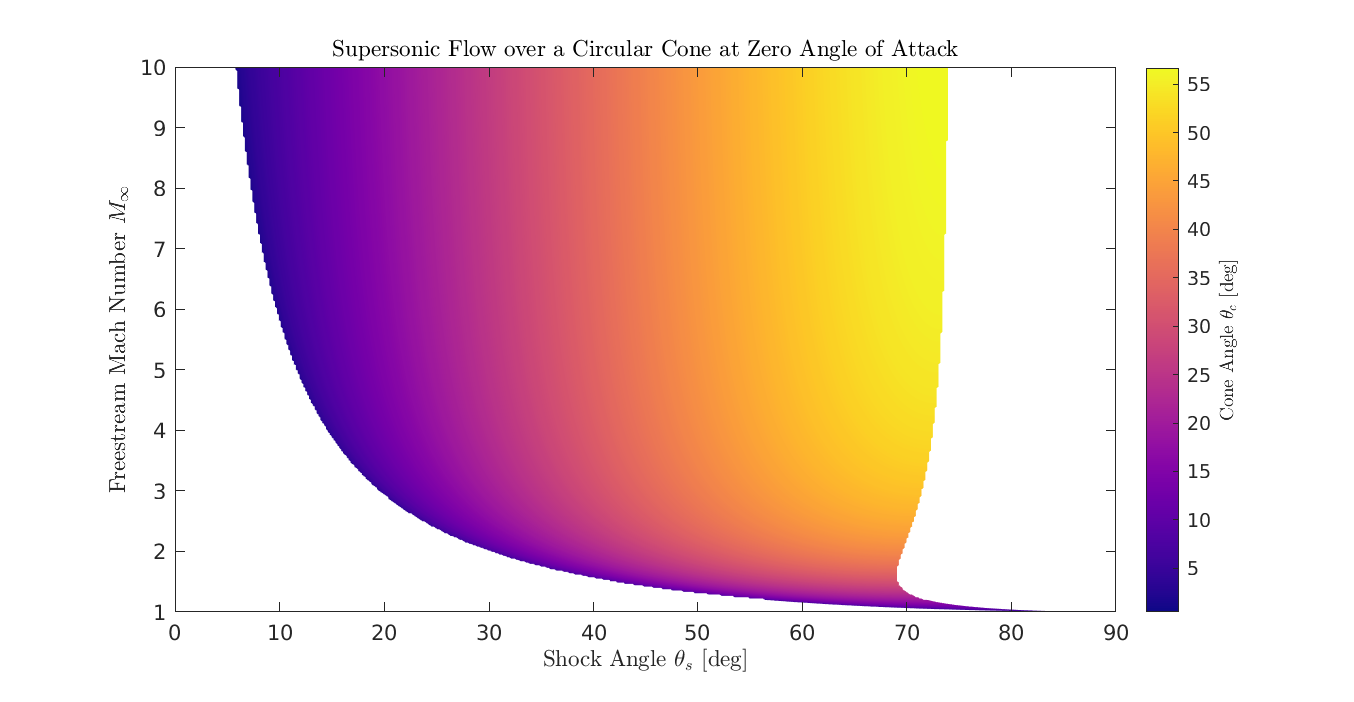
\includegraphics[width=\linewidth]{TheInvTaylorMaccollGrid500x500}
    \caption{QC plot --- Cone half-angle $\theta_c$ (Res: $500 \times 500$).}% Note that solutions to the Taylor-Maccoll equations cease to exist outside to the right of the determined region, indicating a change in the shock pattern of the flow. Solutions outside to the left of the region don't exactly fail to exist, but were simply held to the constraint, $\theta_s < \mu$, where $\mu = \sin^{-1}(1/M)$ is the Mach wave angle.}
    \label{fig:TaylorMaccollQC}
  \end{subfigure}
  \begin{subfigure}[b]{\linewidth}
    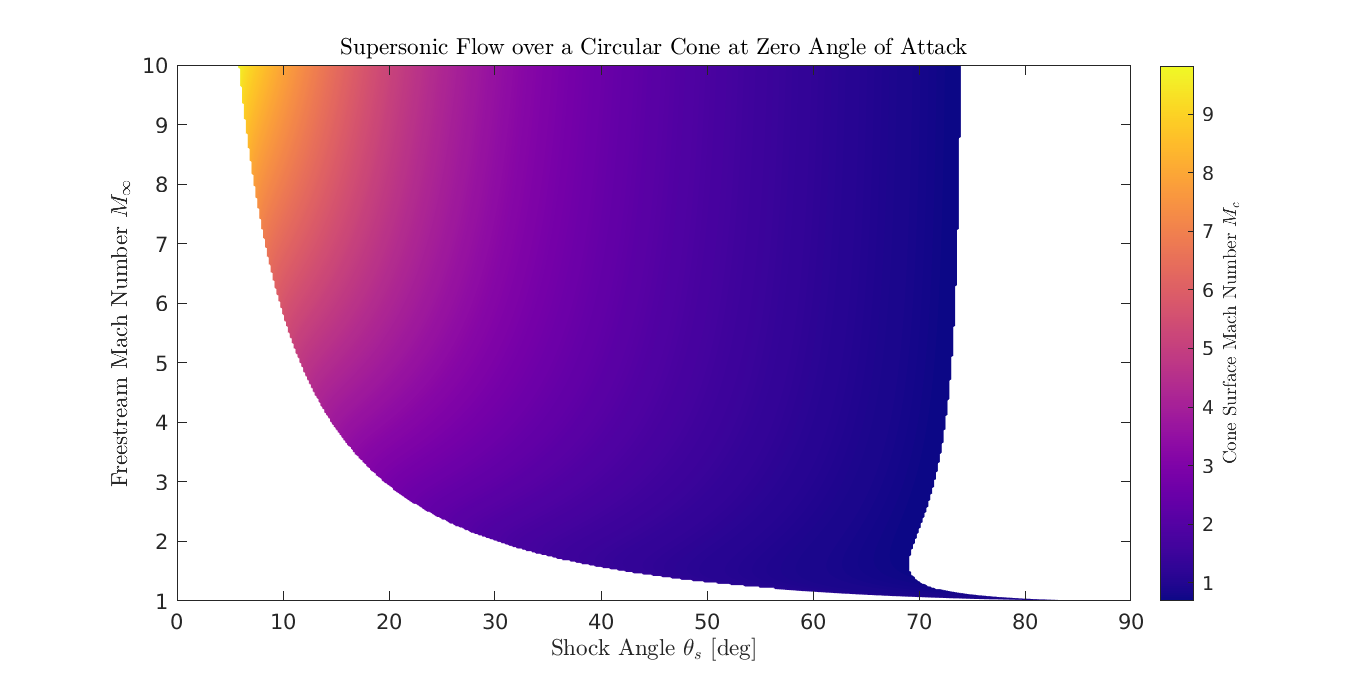
\includegraphics[width=\linewidth]{TheInvTaylorMaccollGridMc500x500}
    \caption{QM plot --- Mach number along the cone's surface $M_c$ (Res: $500 \times 500$).}% Note that solutions to the Taylor-Maccoll equations cease to exist outside to the right of the determined region, indicating a change in the shock pattern of the flow. Solutions outside to the left of the region don't exactly fail to exist, but were simply held to the constraint, $\theta_s < \mu$, where $\mu = \sin^{-1}(1/M)$ is the Mach wave angle.}
    \label{fig:TaylorMaccollQM}
  \end{subfigure}
  \caption{Q plots --- numerical solutions to the Taylor-Maccoll equations up to Mach $10$.}
  \label{fig:TaylorMaccollQ}
\end{figure}
\noindent
Fig. \ref{fig:TaylorMaccollQ} here is said to comprise the Q-plots, or the \textit{inverted} Taylor-Maccoll solutions. The term ``inverted'' refers to the fact that the solutions are functions of the freestream Mach number $M_\infty$ and the shock angle $\theta_s$.

In the context of rockets, it would be most convenient to swap the dependency on the shock angle for the cone's half-angle (a fixed design parameter). However, numerically manipulating the Q-solutions is an insufficient method since the shock angles are well-ordered, but the cone angles and surface Mach numbers are not. Thus, the Q-plots (specifically, the QC-plot) are used as a means to expedite obtaining the O-plots, or the \textit{righted} (or \textit{regular}) Taylor-Maccoll solutions, shown in Figs. \ref{fig:TaylorMaccollUS} and \ref{fig:TaylorMaccollUM}.
\begin{figure}[H]
  \centering
  \begin{subfigure}[b]{\linewidth}
    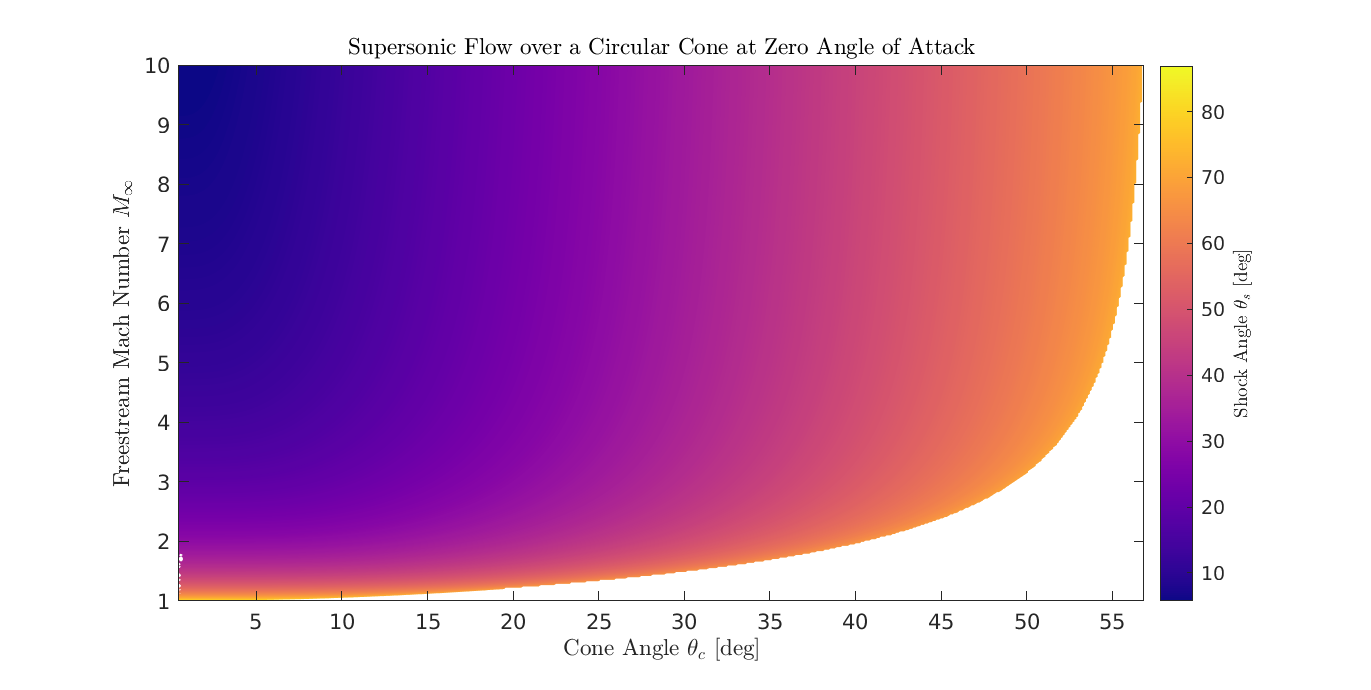
\includegraphics[width=\linewidth]{TheTaylorMaccollGridOs500x500}
    \caption{US plot --- Shock angle $\theta_s$ (Res: $500 \times 500$).}% Note that solutions to the Taylor-Maccoll equations cease to exist outside to the right of the determined region, indicating a change in the shock pattern of the flow. Solutions outside to the left of the region don't exactly fail to exist, but were simply held to the constraint, $\theta_s < \mu$, where $\mu = \sin^{-1}(1/M)$ is the Mach wave angle.}
    \label{fig:TaylorMaccollUS}
  \end{subfigure}
  \begin{subfigure}[b]{\linewidth}
    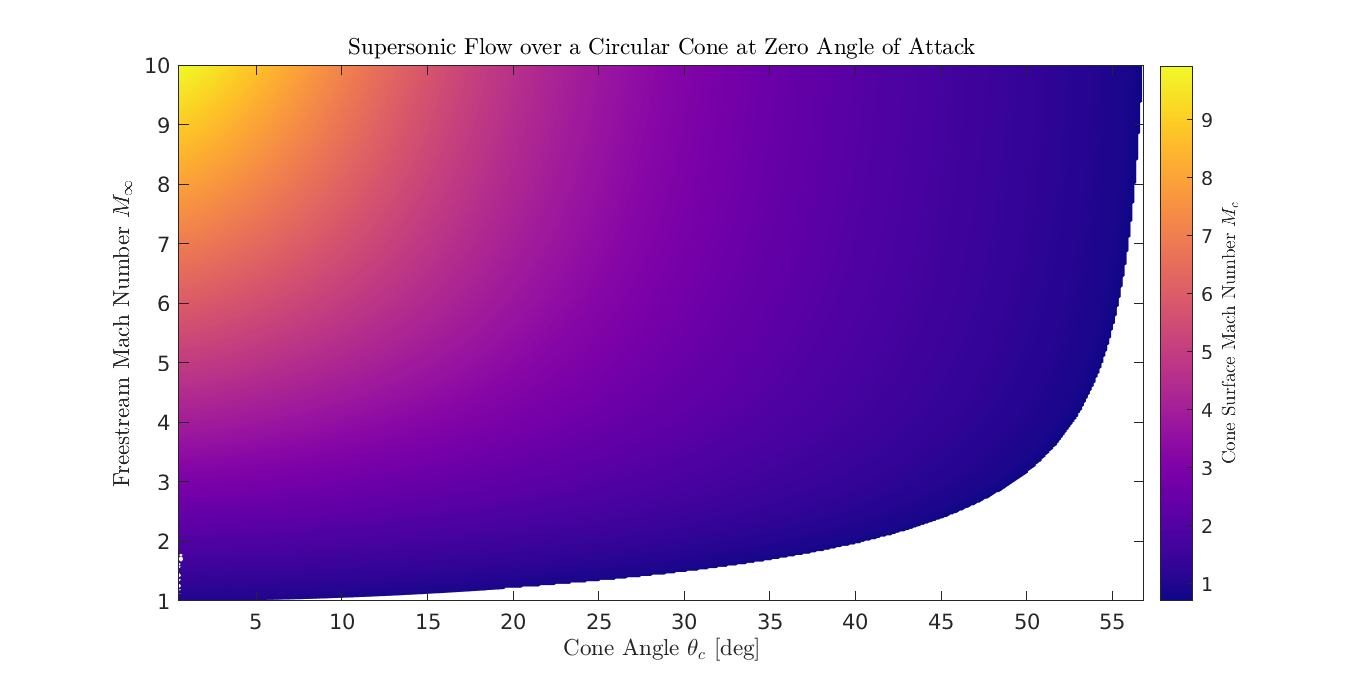
\includegraphics[width=\linewidth]{TheTaylorMaccollGridMc500x500}
    \caption{UM plot --- Mach number along the cone's surface $M_c$ (Res: $500 \times 500$).}% Note that solutions to the Taylor-Maccoll equations cease to exist outside to the right of the determined region, indicating a change in the shock pattern of the flow. Solutions outside to the left of the region don't exactly fail to exist, but were simply held to the constraint, $\theta_s < \mu$, where $\mu = \sin^{-1}(1/M)$ is the Mach wave angle.}
    \label{fig:TaylorMaccollUM}
  \end{subfigure}
  \caption{U plots --- numerical solutions to the Taylor-Maccoll equations up to Mach $10$.}
  \label{fig:TaylorMaccollU}
\end{figure}
\noindent
The U plots simply swap $\theta_s$ for $\theta_c$ from Figs. \ref{fig:TaylorMaccollQ} in an orderly fashion. 

An observation of the QC solution reveals that contours terminate normally on the right-side boundary, indicating that, along this curve, the attached shock detatches and forms a bow shock. Thus, the flow analysis of the Taylor-Maccoll equations concerns the study of \textit{weak} shocks. Such shocks are more commonly encountered than the strong (bow) shocks for circular cones [Anderson]. 
Furthermore, cones having any half-angle greater than about $56^\circ$ will \textit{always} have a strong shock in supersonic flow.
The Q plots both exhibit a boundary on the left-side as well which was a numerical tool blocking shocks from surpassing the Mach angle --- that is, solutions of the form $\theta_s > \mu$, where $\mu$ is the Mach angle defined
\begin{equation}
\mu = \sin^{-1}\frac{1}{M},
\end{equation}
were not considered.

Note that in the U plots, the right-most boundary of the $Q$ plots persists and is remapped into a new boundary separating the weak shock solutions from the strong ones, but the left-most boundary of the Q plots has been eliminated. Also, some small regions between Mach 1 and 2 for the lowest cone angles has some missing data, likely due to computational error. These few points do not represent unphysical flow and may be safely interpolated (locally) to gain determined values.

Knowing the flow behavior as a function of freestream Mach number $M_\infty$ and cone angle $\theta_c$ easily yields the shock angle $\theta_s$, which gives means to evaluating (\ref{eq:AerodynamicsObliqueShockrho}), (\ref{eq:AerodynamicsObliqueShockp}), and (\ref{eq:AerodynamicsObliqueShockT}) if wanting to know the entire flow field, but more importantly provides a direct mapping to stagnation pressure everywhere behind the shock by combining (\ref{eq:AerodynamicsObliqueShockp}) with (\ref{eq:SupersonicFlowPressure}), forming the relation
\begin{equation}
p_{0,d} = p_\infty\left(1 + \frac{2\gamma}{\gamma + 1}(M_\infty^2 \sin^2\theta_s - 1)\right)\left(1 + \frac{\gamma - 1}{2} M_d^2\right)^{\!\frac{\gamma}{\gamma - 1}},
\end{equation}
(where $M_d^2$ is the quantity from (\ref{eq:AerodynamicsMachNumberObliqueShockCone}) using $V' = V'(\theta_s)$, i.e. the nondimensional velocity obtained from the Taylor-Maccoll solution immediately behind the shock) such that the pressure behind the shock is given again by (\ref{eq:AerodynamicsObliqueShockp}) as
\begin{equation}
p_c = p_{0,d}\left(1 + \frac{\gamma - 1}{2} M^2\right)^{\!-\frac{\gamma}{\gamma - 1}}
\end{equation}
\textit{and} the Mach number on the surface of the cone as shown in Fig. \ref{fig:TaylorMaccollUM}. Thus, the pressure on the cone's surface, $p_c$ is finally known and furthermore, is constant.

In this case, the pressure is constant and evenly distributed over the entirety of the cone's surface.

The Taylor-Maccoll flow field is visualized in terms of pressure for clarity.
\begin{figure}[H]
  \centering
  \begin{subfigure}[b]{\linewidth}
    \includegraphics[width=\linewidth]{{PressureRatio8degreeconeMach1.01885}.eps}
    \caption{Mach 1.02 flow over an $8^\circ$ circular cone to show the shockwave and flow field pattern.}% Note that solutions to the Taylor-Maccoll equations cease to exist outside to the right of the determined region, indicating a change in the shock pattern of the flow. Solutions outside to the left of the region don't exactly fail to exist, but were simply held to the constraint, $\theta_s < \mu$, where $\mu = \sin^{-1}(1/M)$ is the Mach wave angle.}
    \label{fig:TaylorMaccollFlowField8DegatMach1_02}
  \end{subfigure}
\end{figure}%
\begin{figure}[H]\ContinuedFloat
  \begin{subfigure}[b]{\linewidth}
    \includegraphics[width=\linewidth]{{PressureRatio20degreeconeMach2.5}.eps}
    \caption{Mach 2.5 flow over a $20^\circ$ circular cone. The pressure on the cone's surface is nearly double that of the freestream.}% Note that solutions to the Taylor-Maccoll equations cease to exist outside to the right of the determined region, indicating a change in the shock pattern of the flow. Solutions outside to the left of the region don't exactly fail to exist, but were simply held to the constraint, $\theta_s < \mu$, where $\mu = \sin^{-1}(1/M)$ is the Mach wave angle.}
    \label{fig:TaylorMaccollFlowField20DegatMach2_5}
  \end{subfigure}
  \caption{Pressure behind the shock relative to the freestream pressure for some sample cones.}
  \label{fig:TaylorMaccollFlowFields}
\end{figure}
The white region is the cone itself (a two-dimensional conical region, not to be confused with a two-dimensional wedge-like region), the uniform region to the left of the stark discontinuity (the shock) is the freestream, and in between is the flow behind the shock. 
%Note its symmetry and the characteristic lines on which the flow field is constant. 
Though shown two-dimensionally, the solution is naturally three-dimensional with rotational symmetry about the $x$ axis. Both $x$ and $y$ are shown without units since the cone is semi-infinite, so the notion of distance here has no meaning.
Finally, note that, generally, the shallower the cone for a constant Mach number, the weaker the shock, so the closer the flow properties behind the shock are to the freestream.

%\begin{figure}[H]
%\centering
%	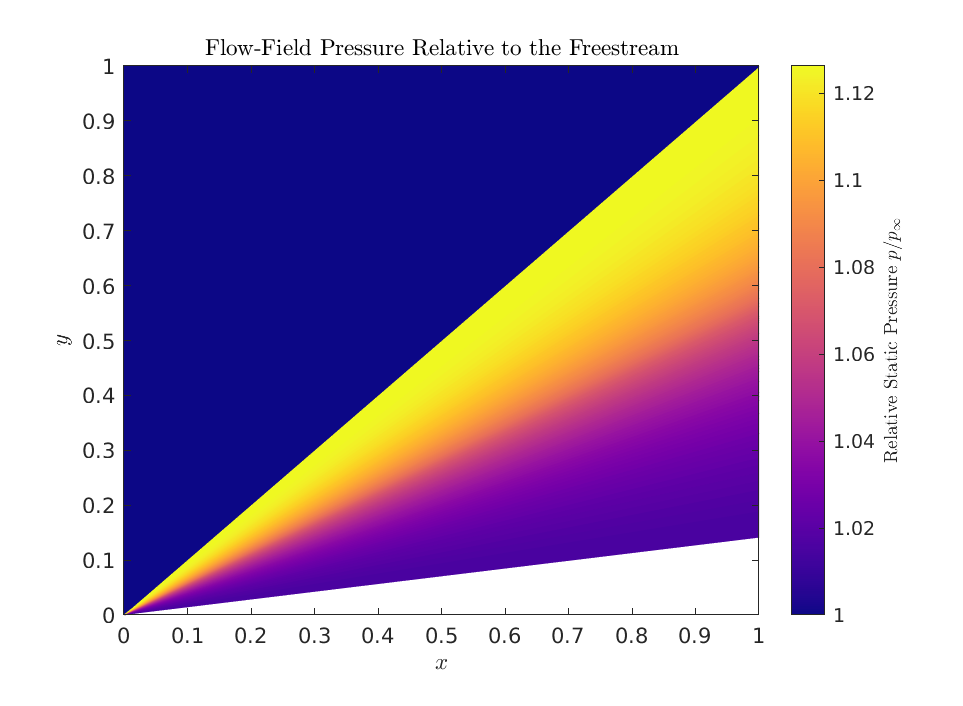
\includegraphics[width=\linewidth]{MaximumPressureDistributionMach1425_8DegreeCone}
%\end{figure}



\subsection{Second-Order Shock-Expansion Theory --- Relation to Curved Nose Cones}
A curved nose cone may be approximated as a circular cone followed by a series of circular frustums such that the nose cone's outline is closely followed. More precisely, a curved nose cone may be approximated by a series of circular cones tangent at various points along the curved body. In this case, the front cone and following frustums are of finite length. 
\begin{figure}[H]
  \centering
  \begin{subfigure}[b]{0.49\linewidth}
    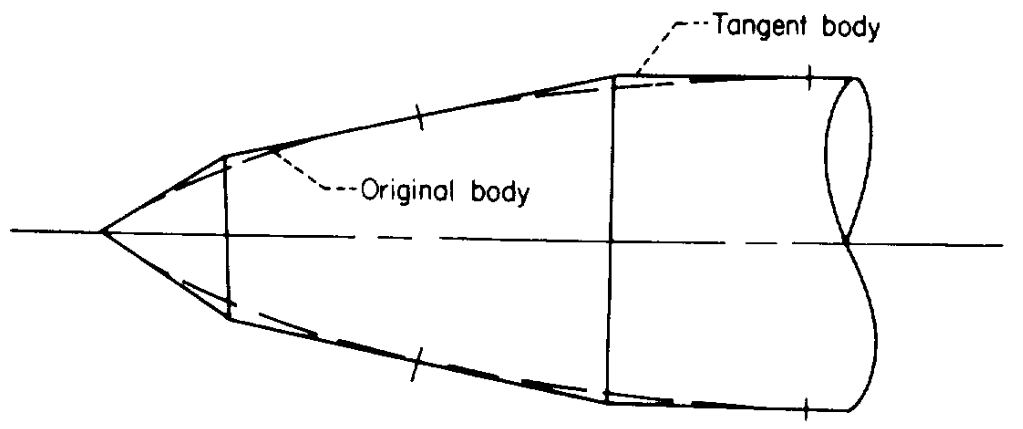
\includegraphics[width=\linewidth]{ASecondOrderShockExpansionMethodOriginalBody}
    \caption{Comparison between the original body and the tangent approximation.}
    \label{fig:AerodynamicsSecondOrderOriginalBody}
  \end{subfigure}
  \begin{subfigure}[b]{0.49\linewidth}
    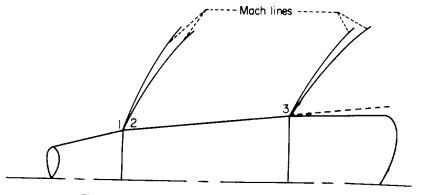
\includegraphics[width=\linewidth]{ASecondOrderShockExpansionMethodTangentBody}
    \caption{The tangent body in supersonic flow with Mach waves emanating from its convex corners.}
    \label{fig:AerodynamicsSecondOrderTangentBody}
  \end{subfigure}
  \caption{Tangent body approximation to the original curved body using a cone and multiple conical frustums and the depiction of the points (corners) $1$, $2$, and $3$, which lie on the tangent body's surface so that the straightforward Prandtl-Meyer relations may be used around the convex corners. Images from NASA TR1328 (Syvertson and Dennis).}
  \label{fig:AerodynamicsSecondOrderBodies}
\end{figure}


Second-order shock-expansion theory from NASA Technical Report 1328 (\textit{A Second-Order Shock-Expansion Method Applicable to Bodies of Revolution Near Zero Lift}) indicates for such conical flows that the pressure over a tangent conical frustum (for $x_2 \leqslant x \leqslant x_3$, where $x_2$ and $x_3$ are the locations of (convex) corners between frustums. In such a case, $x_0 = 0$ may be taken as the initial coordinate if the segment is the leading cone) is
\begin{equation}
p_{23}(x) = p_{23,c} - (p_{23,c} - p_2) \mathrm{e}^{-\eta_{23}(x)}, \label{eq:AerodynamicsSecondOrderp23}
\end{equation}
where $p_{23,c}$ is the pressure on the surface of frustum 2-3's equivalent semi-infinite cone satisfying the Taylor-Maccoll equations, $p_2$ is the pressure on the surface immediately following the expansion fans (which are isentropic processes, so the stagnation pressure from the initial cone is constant throughout) through the 1-2 corner, and
\begin{equation}
\eta_{23}(x) = \left(\frac{\partial p_{23}}{\partial s}\right)_{\!2} \frac{(x - x_2)\sec\theta_{c,2}}{p_{23,c} - p_2}.
\end{equation}
Here, 
%$\delta_i$ is the angle between the frustum's surface and the horizontal 
%(the frustum angle --- in fact, the cone angle for the $i$th frustum's equivalent semi-infinite cone, $\delta_i = $)
the pressure gradient along the frustum's surface is given
\begin{equation}
\left(\frac{\partial p_{23}}{\partial s}\right)_{\!2} = \frac{B_2}{r_{23}(x)}\left(\frac{\Omega_1}{\Omega_2} \sin\theta_{c,1} - \sin\theta_{c,2}\right) + \frac{B_2 / B_1}{\Omega_2 / \Omega_1}\left(\frac{\partial p_{01}}{\partial s}\right)_{\!1},
\end{equation}
where further, for $k = 1,2$ (integer $k$ in general, for frustums to come),
\begin{align}
B_k = \frac{\gamma / 2}{1 - 1 / M_k^2} \,p_k, && \Omega_k = \frac{1}{M_k}\left(\frac{2 + (\gamma - 1)M_k^2}{\gamma + 1}\right)^{\!\frac{1}{2}\frac{\gamma + 1}{\gamma - 1}} \label{eq:AerodynamicsSecondOrderBandOmega}
\end{align}
are constants and $r(x)$ is simply the radius (distance) of the frustum from the longitudinal axis $x$. The value $(\partial p_{01} / \partial s)_1$ is very simply zero for the initial cone (which forms the vertex) since the Taylor-Maccoll pressure and Mach number (flowing over the 0-1 cone) along the surface is constant. 

The Mach number $M_2$ may be evaluating by inverting the Prandtl-Meyer equations, (\ref{eq:PropulsionPrandtlMeyer}) and (\ref{eq:PropulsionPrandtlMeyerFunction}), since the flow deflection angle ($\theta = \theta_{c,1} - \theta_{c,2}$) and upstream Mach number ($M_{r,u} = M_1$) are known. The relation follows
\begin{align}
M_2 = \nu^{-1}\big(\nu(M_1) + \theta\big).
\end{align}
This inverse relation is obtained to within 0.01\% accuracy of the exact result [Carmichael, Hall] as
\begin{equation}
M_2 = \frac{1 + A y + B y^2 + C y^3}{1 + D y + E y^2} \qquad\quad \left(y = \left(\frac{\nu}{\nu_\infty}\right)^{\!2/3} \text{ and } \nu_\infty = \frac{\pi}{2}\big(\sqrt{6} - 1\big)\right),
\end{equation}
where the constants for perfect air in which $\gamma = 7/5$ are
\begin{align}
A = 1.3604 && B = 0.0962 && C = -0.5127 && D = -0.6722 && E = -0.3278.
\end{align}
In this case, the quantity $\nu$ used within $y$ is exactly $\nu = \nu(M_1) + \theta_{c,1} - \theta_{c,2} \geqslant 0$ since $\nu(M_1) \geqslant 0$ and $\theta_{c,1} \geqslant \theta_{c,2}$.



The pressure is now known over the surface of the frustum for which the pressure gradient at $x_3$ may be obtained by directly differentiating (\ref{eq:AerodynamicsSecondOrderp23}) with respect to the surface coordinate $s$, to get
\begin{equation}
\left(\frac{\partial p_{23}}{\partial s}\right)_{\!3} = \frac{p_{23,c} - p_3}{p_{23,c} - p_2} \left(\frac{\partial p_{23}}{\partial s}\right)_{\!2},
\end{equation}
where of course $p_3 = p_{23}(x_3)$.

Indices are simply cycled by \underline{two} when the pressure over a frustum is found. The next frustum ($x_4 \leqslant x \leqslant x_5$, where $x_4$ is on the other side of the expansion fan starting at $x_3$ (despite the fact that these points are actually the same, $x_3 = x_4$) and $x_5$ is at the end of that next frustum in Fig. \ref{fig:AerodynamicsSecondOrderTangentBody}), the equations for the pressure on the surface become
\begin{equation}
p_{45}(x) = p_{45,c} - (p_{45,c} - p_4) \mathrm{e}^{-\eta_{45}(x)},
\end{equation}
where 
\begin{align}
\eta_{45}(x) &= \left(\frac{\partial p_{45}}{\partial s}\right)_{\!4} \frac{(x - x_4) \sec\theta_{c,4}}{p_{45,c} - p_4} \\
\left(\frac{\partial p_{45}}{\partial s}\right)_{\!4} &= \frac{B_4}{r_{45}(x)}\left(\frac{\Omega_3}{\Omega_4} \sin\theta_{c,3} - \sin\theta_{c,4}\right) + \frac{B_4/B_3}{\Omega_4 / \Omega_3} \left(\frac{\partial p_{23}}{\partial s}\right)_{\!3},
\end{align}
and the pressure gradient to be used for the next frustum is
\begin{equation}
\left(\frac{\partial p_{45}}{\partial s}\right)_{\!5} = \frac{p_{45,c} - p_5}{p_{45,c} - p_4} \left(\frac{\partial p_{45}}{\partial s}\right)_{\!4}.
\end{equation}
The quantities $B_k$ and $\Omega_k$ for $k = 4,5$ are evaluated accordingly from (\ref{eq:AerodynamicsSecondOrderBandOmega}). 
The quantities $\theta_{c,i}$ are suggestively the equivalent semi-infinite cone angles, or simply just the angle that the frustum makes with the longitudinal axis. As such, we have trivially that $\theta_{c,2} = \theta_{c,3}$, and as the corners are assumed convex, then $\theta_{c,1} \neq \theta_{c,2}$.

This process continues repeating until the pressure is known across the surfaces of all frustums, at which point, the pressure on the curved nose cone is approximated by the pressures acting on each cone and frustum of the tangent cone.
The final pressure on the tangent cone is 
\begin{equation}
p(x) = \bigcup_{i=0,2,4,\ldots}^N p_{i(i+1)}, \qquad (0 \leqslant x \leqslant L)
\end{equation}
where $N$ is the number of tangent sections used in the approximation and $L = x_{2N - 1}$ (where $x_{2N - 1}$ is the position of the very last corner on the tangent body -- where it meets the body) is the overall nose cone length.

\subsection{Evaluating the Pressure Drag at Zero Angle of Attack}
The integral (\ref{eq:AerodynamicsPressureOnCone}) representing the magnitude of drag on the nose cone due to pressure acting normally on the surface is finally evaluated knowing $p$.
\begin{align}
\iint_{S_n} p \sin\theta_c \,d\hat{S}_n &= \sum_{i = 0,2,\ldots}^N \iint_{S_{n,i}} p \,d\hat{S}_{n,i} \\
&= \sum_{i = 0,2,\ldots}^N \int_0^{2\pi} \int_{r_i}^{r_{i+1}} p(x) \frac{\nabla f}{|\nabla f|} \,dr\,d\phi \\
%&= \sum_{i = 0,2,\ldots}^N \int_0^{2\pi} \int_{r_i}^{r_{i+1}} p(x) \begin{pmatrix}-\cos\phi \cos\theta_c \\ -\sin\phi \cos\theta_c \\ \sin\theta_c\end{pmatrix} \,dr\,d\phi \\
&= \sum_{i = 0,2,\ldots}^N 2\pi \int_{r_i}^{r_{i+1}} p(r\tan\theta_{c,i}) \sin\theta_c \begin{pmatrix}1 & 0 & 0\end{pmatrix}^\mathsf{T} \,dr \\
&= \sum_{i = 0,2,\ldots}^N 2\pi\hat{v} \int_{r_i}^{r_{i+1}} p(r\tan\theta_{c,i}) \sin\theta_c \,dr.
\end{align}
Thus, the force enacted by the pressure on the tangent cone surfaces may readily be carried out by numerical integration. This procedure provides a better estimate of the amount of drag experienced on the rocket's nose, an important quantity when aiming to launch cheaply into the mesosphere or thermosphere, than simply estimating that the pressure acting on the nose is the freestream pressure. In many, if not the vast majority, of cases involving supersonic flow, the nose cone pressure is nowhere near the freestream pressure. Thus, such a treatment with shock-expansion theory seems to be of high importance.





\chapter{Phases of Flight}
\section{Prelaunch}
A rocket, whether intended for purely atmospheric flight or insertion into orbit, launches from a nearly upright position, held in place only by the \textit{launch tower}, which, depending on the size of the rocket, may or may not be situated on a \textit{launch pad}. For smaller rockets, the launch tower might resemble a (straight) rod (on the order of several meters long) called the \textit{guide rail} along which the rocket slides upon motor ignition.

Before liftoff occurs, however, the rocket is statically situated. As such, the rocket is held in place by the launch pad (or ground) \textit{and} the tower in general. Suppose the rocket is of mass $m$ and the gravity model is $g$ (taken to be (\ref{eq:LocalGravity}), (\ref{eq:SpheroidGravityAth}), or (\ref{eq:GravitationalAccelSPHR})). 
Further suppose that the rocket rests on the guide rail which is offset from the local direction of gravity by an angle $\delta$ and offset from the ENV basis component $\widehat{E}$ by the positive (counterclockwise) angle $\psi$ about the $\widehat{V}$ element. 
Then the static forces imposed onto the rail guide are
\begin{align}
F_P = mg\cos\delta, && F_N = mg\sin\delta, \label{eq:PrelaunchStaticForces}
\end{align}
where $F_P$ is the force statically supporting the rocket directed along the rail direction and $F_N$ is the force statically supporting the rocket normal to the rail direction directed through the rocket's body.
These quantities naturally vanish shortly after ignition since the rocket is powerful enough to get itself off of the rail and into free-flight.

The frame created by this 3-rotation from the ENV frame is the \textit{firing frame}, or \textit{local frame}, defined by basis elements $\{\hat{e}_d, \hat{e}_c, \hat{e}_u\}$ which are related to the ENV elements $\{\widehat{E}, \widehat{N}, \widehat{V}\}$ via (\ref{eq:ElementalRotz}). As such, the coordinate variables are related to one another by
\begin{equation}
\begin{pmatrix}x_d \\ x_c \\ x_u\end{pmatrix} = \underbrace{\begin{pmatrix}\cos\psi & \sin\psi & 0 \\ -\sin\psi & \cos\psi & 0 \\ 0 & 0 & 1\end{pmatrix}}_{\mathbf{T}^{\text{loc}/\text{env}}} \begin{pmatrix}x_{\lambda} \\ x_{\phi} \\ x_{h}\end{pmatrix},
\end{equation}
where $x_d$ is the \textit{downrange} position, $x_c$ is the \textit{crossrange} position, and $x_u$ is the usual vertical height (up) as defined by the ENV frame. 
%
The \textit{launch}, or \textit{rail}, frame has its coordinate components related to that of the local frame by the elemental rotation of having the launch rail differ from true vertical by the angle $\delta$.
\begin{equation}
\begin{pmatrix}\tilde{x}_d \\ \tilde{x}_c \\ \tilde{x}_u\end{pmatrix} = \underbrace{\begin{pmatrix}\cos\delta & 0 & -\sin\delta \\ 0 & 1 & 0 \\ \sin\delta & 0 & \cos\delta\end{pmatrix}}_{\mathbf{T}^{\text{rail}/\text{loc}}} \begin{pmatrix}x_d \\ x_c \\ x_v\end{pmatrix},
\end{equation}

\subsection{Initial Conditions}
A short discussion of the methods used to determine the resulting trajectory of the flight vehicle is proper. The equations of motion dictating the linear motion of the vehicle's mass center are determined via Newton's laws which necessarily yield three (3) coupled, nonlinear, nonhomogeneous, nonautonomous, \textit{second-order} scalar ordinary differential equations. The rigid-body orientation (rotational motion) of the flight vehicle is deduced through Euler's second law, which necessarily yields three (3) coupled, nonlinear, nonhomogeneous, autonomous, \textit{first-order} scalar ordinary differential equations. To connect the orientation of the flight vehicle's body frame with the ENV frame (in which the equations of motion are written) simultaneously (without explicitly knowing the orientation), the quaternion kinematic equation is employed which necessarily yields four (4) coupled, nonlinear, homogeneous, autonomous, \textit{first-order} scalar ordinary differential equations.

Put into phase-space form, there are thirteen (13) first-order differential for which there are 13 initial conditions required. These variables requiring initial conditions describe the initial position of the vehicle's mass center ($x_0$, $y_0$, and $z_0$), the initial velocity of the vehicle's mass center ($\dot{x}_0$, $\dot{y}_0$, and $\dot{z}_0$), the initial angular velocity of the vehicle ($\omega_{10}$, $\omega_{20}$, and $\omega_{30}$), and the quaternions parameterizing the orientation ($q_{10}$, $q_{20}$, $q_{30}$, and $q_{40}$).

Explicitly, $x_0$, $y_0$, and $z_0$ indicate an initial position taken with respect to the ENV frame and $\dot{x}_0$, $\dot{y}_0$, and $\dot{z}_0$ describing the initial velocity are also taken with respect to the ENV frame. The quantities $\omega_{10}$, $\omega_{20}$, and $\omega_{30}$ describe the initial angular velocity of the rigid body about each body-frame axis (1, 2, and 3 defined with the origin at the mass center) with respect to the rail frame. The quaternion components $q_{10}$, $q_{20}$, $q_{30}$, and $q_{40}$ compose the quaternion $q$, where $(q_1, q_2, q_3)$ is the vector component and $q_4$ is the scalar component. The quaternion has the constraint that it must, under all circumstances, be unit normalized.
%Put into phase-space form, there are thirteen (13) first-order differential for which there are 13 initial conditions required. These variables requiring initial conditions describe the initial position of the vehicle's mass center ($x_0$, $y_0$, and $z_0$, where these variables indicate values taken with respect to the ENV frame), the initial velocity of the vehicle's mass center ($\dot{x}$, $\dot{y}_0$, and $\dot{z}_0$, again taken with respect to the ENV frame), the initial angular velocity of the vehicle ($\omega_{10}$, $\omega_{20}$, and $\omega_{30}$, where each describes the initial angular velocity of the rigid body about each body frame axis (1, 2, and 3 defined with the origin at the mass center) with respect to the ENV frame), and 

With a vehicle launching from rest from a launch tower at time $t = 0$, these initial conditions may most easily be expressed as
\begin{align}
x_0 &= 0 & \dot{x}_0 &= 0 & \omega_{10} &= 0 & q_{10} &= 0\\
y_0 &= 0 & \dot{y}_0 &= 0 & \omega_{20} &= 0 & q_{20} &= 0\\
z_0 &= 0 & \dot{z}_0 &= 0 & \omega_{30} &= 0 & q_{30} &= 0\\
    &    &           &    &             &    & q_{40} &= 1.
\end{align}
A more detailed analysis of the initial position reveals that, given the straight-line distance $\delta_r$ between the guide rail's centerline and the rocket's centerline,  
\begin{equation}
\begin{pmatrix}x_0 \\ y_0 \\ z_0\end{pmatrix} = \underbrace{\mathbf{T}^{\text{env}/\text{loc}}\, \mathbf{T}^{\text{loc}/\text{rail}}}_{\mathbf{T}^{\text{env}/\text{rail}}} \begin{pmatrix}\delta_r \\ 0 \\ L_{cmb}\end{pmatrix} = \begin{pmatrix}(L_{cmb}\sin\delta + \delta_r\cos\delta)\cos\psi \\ (L_{cmb}\sin\delta + \delta_r\cos\delta)\sin\psi \\ L_{cmb}\cos\delta - \delta_r\sin\delta\end{pmatrix},
\end{equation}
where $L_{cmb}$ is the distance of the vehicle's mass center from the nozzle ($b$, for bottom). The effect of stating $x_0 = y_0 = z_0 = 0$ is that the rocket is skewered by the launch rail and the rocket's mass center (as opposed to the bottom of the rocket) is placed at its base. Physically, such a simplification amounts to the launch rail being shifted over slightly from its actual location and approximately lengthened by $L_{cmb}$.

In the sense of numerical stability, it may be necessary to perturb the initial velocity slightly. Such a perturbation is physically insignificant if on very small orders of magnitude and successfully avoids division by zero. Alternatively, any directionality associated with motion along the rail is constant and aligned with the rail itself, which completely averts the problem of division by zero in this case.

\subsection{Defining the Body Frame}
The statement that $q_{40} = 1$ initially realizes that the body axis is perfectly aligned with the rail axis at time $t = 0$. Note that the golden axes outlined in Fig. \ref{fig:StructuresRocketNStage} are \underline{\textbf{not}} the body axes. Although the two frames share the same origin (the vehicle's overall center of mass), some axes of the golden frame in Fig. \ref{fig:StructuresRocketNStage} must be switched around such that the body-frame's $1$, $2$, and $3$ axes align \textit{exactly} with the rail's $1$, $2$, and $3$ axes at time $t = 0$. Precisely, the axes must undergo the change of basis
\begin{equation}
\begin{pmatrix}x_{1} \\ x_{2} \\ x_{3}\end{pmatrix} = \underbrace{\begin{pmatrix}0 & 0 & 1 \\ 0 & 1 & 0 \\ -1 & 0 & 0\end{pmatrix}}_{\mathbf{T}^{\text{body}/\text{struc}}} \begin{pmatrix} x \\ y \\ z\end{pmatrix},
\end{equation}
where $(x, y, z)$ reference the structure coordinates defined in Fig. \ref{fig:StructuresRocketNStage} and \textit{not} ECF coordinates here.
\begin{figure}[H]
\centering
\begin{tikzpicture}
% Originally from propulsion section, modified to fit structures discussion
%% Temporary axis (comment out this bit when done)
%\draw[red] (0,0) -- (1,0);
%\draw[red] (0,0) -- (0,1);

% Draw the nozzle
\begin{axis}[width=15cm,
			height=207pt,
			at={(-6.71cm,0pt)},
			xmin=-8.08, xmax=1.25,
			ymin=-15, ymax=10,
			hide axis,
			]

%% Temporary axis (comment out this bit when done)
%\draw[blue] (0,0) -- (1,0);
%\draw[blue] (0,0) -- (0,1);
% Plot the diverging section - must keep curves as trig forms for constants to work (1 is hardcoded)
\pgfmathsetmacro{\YOfNozzleThroat}{1} % 1
\pgfmathsetmacro{\YOfNozzleExit}{2} % 3
\pgfmathsetmacro{\A}{(\YOfNozzleThroat + \YOfNozzleExit) / 2}
\pgfmathsetmacro{\B}{(\YOfNozzleThroat - \YOfNozzleExit) / 2}
%\addplot[domain=0:1, samples=100, smooth, solid]{\A + \B * cos(deg(pi*x))};
%\addplot[domain=0:1, samples=100, smooth, solid]{-\A - \B * cos(deg(pi*x))};
% Plot the converging part
\pgfmathsetmacro{\XOfBodyNozzleIntersection}{-1.25} % -0.25
\pgfmathsetmacro{\YOfBody}{1.5} % 1.25
\pgfmathsetmacro{\C}{(\YOfNozzleThroat + \YOfBody) / 2}
\pgfmathsetmacro{\D}{(\YOfNozzleThroat - \YOfBody) / 2}
\pgfmathsetmacro{\E}{1/\XOfBodyNozzleIntersection}
%\addplot[domain=\XOfBodyNozzleIntersection:0, samples=100, smooth, solid]{\C + \D * cos(deg(\E*pi*x))};
%\addplot[domain=\XOfBodyNozzleIntersection:0, samples=100, smooth, solid]{-\C - \D * cos(deg(\E*pi*x))};
% Plot the body
\pgfmathsetmacro{\XofConeBodyIntersection}{-6}
%\addplot[domain=\XofConeBodyIntersection:\XOfBodyNozzleIntersection, samples=100, smooth, solid]{\YOfBody};
%\addplot[domain=\XofConeBodyIntersection:\XOfBodyNozzleIntersection, samples=100, smooth, solid]{-\YOfBody};
% Fill the body
% Plot the nose as half of an ellipse
\pgfmathsetmacro{\a}{2}
\pgfmathsetmacro{\b}{\YOfBody}
\pgfmathsetmacro{\aInner}{\a-0.125}
\pgfmathsetmacro{\bInner}{\b-0.4}
\pgfmathsetmacro{\XofNoseTip}{\XofConeBodyIntersection-\a}
\pgfmathsetmacro{\XofNoseTipInner}{\XofConeBodyIntersection-\aInner}


% Plot the (elliptical) nose cone with thickness
\addplot[domain=-\YOfBody:\YOfBody, samples=100, smooth, solid, draw=black, postaction={pattern=north east lines, pattern color=black}, variable=\y] ({\XofConeBodyIntersection - \a * sqrt(1 - (\y / \b)^2)}, \y);
% Corrective white layer to remove lines coming out of the back for some reason
\addplot[domain=-\bInner:\bInner, samples=100, smooth, solid, white, fill=white, variable=\y] ({\XofConeBodyIntersection+0.05 - \aInner * sqrt(1 - (\y / \bInner)^2)}, \y);
\addplot[domain=-\bInner:\bInner, samples=100, smooth, solid, fill=white, variable=\y] ({\XofConeBodyIntersection - \aInner * sqrt(1 - (\y / \bInner)^2)}, \y);
% Lead into the body
\pgfmathsetmacro{\plusSpacing}{0.03}
\pgfmathsetmacro{\XofPlusConeBody}{\XofConeBodyIntersection+\plusSpacing}
%\node at (\XofPlusConeBody,0){$+$};
\pgfmathsetmacro{\XofBody}{\XofPlusConeBody+\plusSpacing}
%% Plot the body with thickness
\draw[pattern=north east lines, pattern color=black] (\XofBody,-\YOfBody) rectangle (\XOfBodyNozzleIntersection,-\bInner);
\draw[pattern=north east lines, pattern color=black] (\XofBody,\YOfBody) rectangle (\XOfBodyNozzleIntersection,\bInner);
% Lead into the frustum
\pgfmathsetmacro{\XofPlusBodyFrustum}{\XOfBodyNozzleIntersection+2*\plusSpacing}
%\node at (\XofPlusBodyFrustum+0.05,0){$+$};
\pgfmathsetmacro{\XofFrustumB}{\XofPlusBodyFrustum+\plusSpacing}
% Draw frustum
\pgfmathsetmacro{\XOfFrustumT}{0} % 0.5
\pgfmathsetmacro{\YOfFrustumT}{1.3*\YOfBody}
\pgfmathsetmacro{\YOfFrustumTB}{\YOfFrustumT-\YOfBody+\bInner}
\draw[pattern=north east lines, pattern color=black] (\XofFrustumB, \bInner) -- (\XofFrustumB, \YOfBody) -- (\XOfFrustumT, \YOfFrustumT) -- (\XOfFrustumT, \YOfFrustumTB) -- cycle;
\draw[pattern=north east lines, pattern color=black] (\XofFrustumB, -\bInner) -- (\XofFrustumB, -\YOfBody) -- (\XOfFrustumT, -\YOfFrustumT) -- (\XOfFrustumT, -\YOfFrustumTB) -- cycle;
% Lead into recursion by drawing another body
\pgfmathsetmacro{\XOfNextBody}{\XOfFrustumT + 2.5*\plusSpacing}
\pgfmathsetmacro{\XOfFinal}{\XOfNextBody+1.1}
\draw[pattern=north east lines, pattern color=black] (\XOfNextBody, \YOfFrustumTB) rectangle (\XOfFinal, \YOfFrustumT);
\draw[pattern=north east lines, pattern color=black] (\XOfNextBody, -\YOfFrustumTB) rectangle (\XOfFinal, -\YOfFrustumT);

\pgfmathsetmacro{\YOfXLine}{-\YOfBody-2}
\pgfmathsetmacro{\tickHeight}{1}
\draw (\XofNoseTip, \YOfXLine) -- (\XOfFinal, \YOfXLine);
%\draw[thick] (\XofNoseTip, \YOfXLine-\tickHeight/2) -- (\XofConeBodyIntersection-\a, \YOfXLine+\tickHeight/2); %node[below, yshift=-2.65mm]{$n$}; % yshift=-2.6mm
%\draw[->, thick, >=latex] (\XofNoseTip, \YOfXLine) -- (\XofNoseTip+\a/2.5, \YOfXLine) node[pos=0.3, below]{$\rho_1$} node[pos=1.1, below]{$x_1$};
%%
%\draw[thick] (\XofBody, \YOfXLine-\tickHeight/2) -- (\XofBody, \YOfXLine+\tickHeight/2);
%\draw[->, thick, >=latex] (\XofBody, \YOfXLine) -- (\XofBody+\a/2.5, \YOfXLine) node[pos=0.3, below]{$\rho_2$} node[pos=1.1, below]{$x_2$};
%%
%\draw[thick] (\XofFrustumB, \YOfXLine-\tickHeight/2) -- (\XofFrustumB, \YOfXLine+\tickHeight/2);
%\draw[->, thick, >=latex] (\XofFrustumB, \YOfXLine) -- (\XofFrustumB+\a/2.5, \YOfXLine) node[pos=0.3, below]{$\rho_3$} node[pos=1.1, below]{$x_3$};
%%
%\draw[thick] (\XOfNextBody, \YOfXLine-\tickHeight/2) -- (\XOfNextBody, \YOfXLine+\tickHeight/2);
%\draw[->, thick, >=latex] (\XOfNextBody, \YOfXLine) -- (\XOfNextBody+\a/2.5, \YOfXLine) node[pos=0.3, below]{$\rho_4$} node[pos=1.1, below]{$x_4$};

% Center of Mass marker
\pgfmathsetmacro{\XOfCOM}{-2.15}
\draw (\XOfCOM, \YOfXLine-\tickHeight/2) -- (\XOfCOM, \YOfXLine+\tickHeight/2) node[below, xshift=1mm, yshift=-1mm]{mass center};

% Draw longitudinal axis from nose
\draw[->, >=latex, thick] (\XofNoseTip, 0) -- (\XofNoseTip+0.8, 0) node[right, xshift=-0.5mm]{$\underline{x}$};
\draw[->, >=latex, thick] (\XofNoseTip, 0) -- (\XofNoseTip,3); % node[left]{$\underline{y}$}; % Out of frame
% Draw longitudinal axis from COM
\draw[->, >=latex, thick, yellow!55!black!90] (\XOfCOM, 0) -- (\XOfFinal-0.5, 0) node[black, right, xshift=-0.5mm]{$x$};
%\draw[->, >=latex, thick, yellow!55!black!90] (\XOfCOM, 0) -- (\XOfCOM,3) node[black, left]{$y$};

\draw[->, >=latex, thick, red!55!black!90] (\XOfCOM, 0) -- (-\XOfFinal-3.75, 0) node[black, left, xshift=0.5mm]{$x_{3}$};
\draw[->, >=latex, thick, red!55!black!90] (\XOfCOM, 0) -- (\XOfCOM,3) node[black, left]{$y$} node[black, right]{$x_{2}$};
\end{axis}


%
% Try to draw center of mass
% Nose cone
\begin{scope}[shift={(-4.75, 2.415)}] % (1.2, 2.415)
\pgfmathsetmacro{\Bx}{0}
\pgfmathsetmacro{\By}{1}
\pgfmathsetmacro{\Br}{0.11}
\draw[fill=black] (\Bx,\By) ++(0:\Br)   arc (0:90:\Br)    -- (\Bx,\By) -- cycle;
\draw[fill=white] (\Bx,\By) ++(90:\Br)  arc (90:180:\Br)  -- (\Bx,\By) -- cycle;
\draw[fill=black] (\Bx,\By) ++(180:\Br) arc (180:270:\Br) -- (\Bx,\By) -- cycle;
\draw[fill=white] (\Bx,\By) ++(270:\Br) arc (270:360:\Br) -- (\Bx,\By) -- cycle;
\end{scope}
% Body
\begin{scope}[shift={(-0.2, 2.415)}]
\pgfmathsetmacro{\Bx}{0}
\pgfmathsetmacro{\By}{1}
\pgfmathsetmacro{\Br}{0.11}
\draw[fill=black] (\Bx,\By) ++(0:\Br)   arc (0:90:\Br)    -- (\Bx,\By) -- cycle;
\draw[fill=white] (\Bx,\By) ++(90:\Br)  arc (90:180:\Br)  -- (\Bx,\By) -- cycle;
\draw[fill=black] (\Bx,\By) ++(180:\Br) arc (180:270:\Br) -- (\Bx,\By) -- cycle;
\draw[fill=white] (\Bx,\By) ++(270:\Br) arc (270:360:\Br) -- (\Bx,\By) -- cycle;
\end{scope}
% Frustum
\begin{scope}[shift={(4.3, 2.415)}]
\pgfmathsetmacro{\Bx}{0}
\pgfmathsetmacro{\By}{1}
\pgfmathsetmacro{\Br}{0.11}
\draw[fill=black] (\Bx,\By) ++(0:\Br)   arc (0:90:\Br)    -- (\Bx,\By) -- cycle;
\draw[fill=white] (\Bx,\By) ++(90:\Br)  arc (90:180:\Br)  -- (\Bx,\By) -- cycle;
\draw[fill=black] (\Bx,\By) ++(180:\Br) arc (180:270:\Br) -- (\Bx,\By) -- cycle;
\draw[fill=white] (\Bx,\By) ++(270:\Br) arc (270:360:\Br) -- (\Bx,\By) -- cycle;
\end{scope}
% COM
\begin{scope}[shift={(1.83, 2.415)}] 
\pgfmathsetmacro{\Bx}{0}
\pgfmathsetmacro{\By}{1}
\pgfmathsetmacro{\Br}{0.11}
\draw[fill=black] (\Bx,\By) ++(0:\Br)   arc (0:90:\Br)    -- (\Bx,\By) -- cycle;
\draw[fill=red!55!black!90] (\Bx,\By) ++(90:\Br)  arc (90:180:\Br)  -- (\Bx,\By) -- cycle;
\draw[fill=black] (\Bx,\By) ++(180:\Br) arc (180:270:\Br) -- (\Bx,\By) -- cycle;
\draw[fill=yellow!55!black!90] (\Bx,\By) ++(270:\Br) arc (270:360:\Br) -- (\Bx,\By) -- cycle;
\end{scope}

%% Label y_n here to maximize rocket in plot
\node at (-6.85, 4.05){$\underline{y}$}; % y_n -> -6.9 | \underbace{y} -> 4.05 instead of 4.1

\end{tikzpicture}
\caption{Differentiating the structure-frame (struc) in gold and the body-frame (body) in red. The $x_1$ direction in the body-frame is directed outwards such that the right-hand rule is satisfied. When on the the launch rail, the $x_1$ direction is pointing downrange as in the local frame except angled downwards by $\delta$.}
\label{fig:PreLaunchBodyFrame}
\end{figure}
With this change of basis, the moment of inertia matrix must also be transformed into the body-frame (which is still a principal axis frame) according to
\begin{equation}
[I]^{\text{body}} = \mathbf{T}^{\text{body}/\text{struc}} \,[I]^\text{struc}\,\mathbf{T}^{\text{struc}/\text{body}},
\end{equation}
where $[I]^\text{struc}$ is the mass moment of inertia matrix computed as outlined in Ch. \ref{ch:Structures}; its original notation followed (\ref{eq:StructuresMoIStructureFrame}) where it held the symbol $[I]$, but this quantity is \textit{not} the same as the moment of inertia matrix expressed in the body-frame $[I]^{\text{body}}$. The derivative likewise follows suit since this transformation is constant in time.
\begin{equation}
\frac{d[I]^{\text{body}}}{dt} = \mathbf{T}^{\text{body}/\text{struc}} \,\frac{d[I]^\text{struc}}{dt}\,\mathbf{T}^{\text{struc}/\text{body}}.
\end{equation}

\section{Rail-Guided Flight}
Supposing it produces a sufficient amount of thrust to overcome its own weight shortly after ignition, the rocket begins traversing up and along the launch/guide rail. There are \textit{two} distinct regions of interest during this brief period of time before the rocket begins true unguided flight. These regions are distinguished by two corresponding periods of time within the overall time between launch and rail clearance. 

The first region is defined from ignition until the nose just begins to break through the rail guide's end (i.e. while the entire rocket is fully contained along the rail). The other region follows immediately after the first and is defined until the active nozzle clears the rail (i.e. while the rocket is leaving the rail and, therefore, transitioning from rail-guided flight to free-flight).
\subsection{Fully Rail-Guided Flight}
The static forces imposed on the rail (\ref{eq:PrelaunchStaticForces}) are generalizable to include the dynamic effect of thrust.
\begin{align}
F_P = \max(0, mg\cos\delta - F_T), && F_N = mg\sin\delta. \label{eq:FullyRailGuidedFlightRailForces}
\end{align}
Here, $\delta$, the angle between the direction of the launch rail and the local vertical direction $\widehat{V}$, is assumed to be small. Thus, the rocket doesn't move if $F_T \leqslant mg\cos\delta$ by physical intuition since $F_P \geqslant 0$ is still supporting some amount of the rocket's weight. Otherwise, the rail supports no weight along the rail direction and the rocket traverses up along the rail.
The direction of motion is essentially constant since the vehicle is securely attached to sliding guides along the rail. Thus, any effects of wind are ignored during the phase.
The effects of friction during this period of time are also assumed negligible to the amount of thrust and subsequently ignored.

\subsubsection{Dynamic Forces}
Despite the low speeds involved in this phase, aerodynamic forces begin to develop with the introduction of nonzero velocity due to nonzero thrust. The linear acceleration of the vehicle along the direction of the rail is
\begin{equation}
\vec{F}_{1.1}^{\text{rail}} = \begin{pmatrix}0 \\ 0 \\ F_T - F_D - mg\cos\delta\end{pmatrix}
\end{equation}
which is expressed with respect to the ENV frame as
\begin{equation}
\vec{F}_{1.1}^{\text{env}} = \mathbf{T}^{\text{env}/\text{rail}} \vec{F}_{1.1}^{\text{rail}}.
%= \begin{pmatrix}(F_T - F_D - mg\cos\delta)\sin\delta\cos\psi \\ (F_T - F_D - mg\cos\delta)\sin\delta\sin\psi \\ (F_T - F_D - mg\cos\delta)\cos\delta \end{pmatrix}
\end{equation}
The vehicle mass $m$ is inherently is a function of time since propellant is being expelled from the system in the form of exhaust. In the most general manner, the mass is written
\begin{equation}
m = m_0 + \int_0^t \dot{m}(s)\,ds,
\end{equation}
where $m_0$ is the initial mass of the vehicle as measured before launch, $\dot{m} \leqslant 0$ is the mass flow rate (a known function of time), and $0 \leqslant t \leqslant t_f$ is the current flight time. During the first stage which, of course, is assumed to be able to clear the rail sufficiently before burning out at time $t_b$, we can restrict $\dot{m} < 0$ and $0 \leqslant t \leqslant t_b$ to reflect the fact that the vehicle is firing, where $t_b$ is the burnout time.
If precise knowledge of $\dot{m}$ is unknown while firing, then a basic estimate may be made of linear form
\begin{equation}
\dot{m} \sim \frac{m_f - m_0}{t_b},
\end{equation}
where the quantity $m_f - m_0$ represents the entire mass of the propellant used during the first stage.

There are no torques acting on the center of mass since the vehicle is constrained to move along the rail. The angular rates and orientation, therefore, remain constant during this phase.

\subsection{Partially Rail-Guided Flight}
An approximate expression for the forces imposed on the guide rails while the rocket is transitioning to free-flight can be written as a generalization upon (\ref{eq:FullyRailGuidedFlightRailForces}) by linearly introducing a scaling as
\begin{align}
F_P = \max(0, mg\cos\delta - F_T), && F_N = \eta mg\sin\delta.
\end{align}
Here, $\eta$ is a measure of the length of the rocket still in contact with the rail given by
\begin{equation}
\eta = \min\left(\max\left(0,\, \frac{L_{tower} - (r_{cmp} - L_{cmb})}{L}\right),\, 1\right),
\end{equation}
where $L$ is the length of the entire flight vehicle, $L_{cmb}$ is as previously defined, $L_{tower}$ is the length of the launch tower from base to tip, and $r_{cmp}$ is the position of the rocket's center of mass as measured from a position parallel along the rail. To account for this subtle shift in coordinates (due to the launch rail being deflected by the angle $\delta$ from the vertical direction $\widehat{V}$), $r_{cmp} \geqslant 0$ is written
\begin{equation}
r_{cmp}^2 = (x_\lambda + \delta_r\sin\mathrm{El})^2 + x_\phi^2 + (x_h - \delta_r\cos\mathrm{El})^2,
\end{equation}
where $\delta_r$ is the straight-line distance separating the centerline of the launch rail from the centerline of the rocket and $\mathrm{El}$ is the rocket's \textit{elevation} (usually paired with an \textit{azimuth} $\mathrm{Az}$) given
\begin{align}
\tan\mathrm{Az} = \frac{x_\lambda}{x_\phi} && \sin\mathrm{El} = \frac{x_h}{r_{env}}.
\end{align}
The quantity $r_{env} \geqslant 0$ here is simply the distance of the rocket's mass center from the ENV origin.
\begin{equation}
r_{env}^2 = {x_\lambda^2 + x_\phi^2 + x_h^2}
\end{equation}
Note that this combination of $\mathrm{Az}$, $\mathrm{El}$, and $r_{env}$ provides a means to measure position much like spherical coordinates, where $\mathrm{Az}$ is measured from true north (whose direction is given by $\widehat{N}$) and $\mathrm{El}$ is measured from the east--north plane where $\mathrm{El} > 0$ corresponds to a positive height above the ground. 
%Both azimuth and elevation are defined only locally to the ENV frame, which consists of the east--north plane tangent to the ellipsoid at $(\lambda, \phi, 0)$.

\subsubsection{Weathervaning}
Though lasting only momentarily, the vehicle's flight speed is relatively slow upon transitioning into and entering free-flight. During this time, the vehicle is susceptible to \textit{weathervaning}, or \textit{weathercocking}. That is, the wind speed is comparable to rocket's velocity during this time which is able to cause a slight alteration in its nominal launching direction. A blowing wind with wind speed $w$ induces an angle of attack $\alpha_{wv}$ on the vehicle given by
\begin{equation}
\tan\alpha_{wv} = \frac{w}{v},
\end{equation}
where $v$ is the speed of the vehicle (as expressed in the ENV frame, which is consistent with the expression of $w$). Here, the 2-argument arctangent function is unnecessary; the usual arctangent function may be safely employed.

As a result of the induced angle of attack, an aerodynamic force is generated about the vehicle's center of pressure \textit{in the direction of the wind} which, in general, causes a nonzero torque about the vehicle's center of mass. Consequently, the vehicle turns the angle $\alpha_{wv}$ \textit{into} the direction of the wind and necessarily fails to reach its maximum altitude if launched in a perfectly vertical configuration [NASA GRC].

For much slower flight vehicles, this effect may persist much further into the flight, well beyond the point of exiting the launching platform.

\subsubsection{Dynamic Forces}
All aerodynamic forces act through the center of pressure, which, in general, differs in location from the center of mass. 
The location of the vehicle's center of pressure is given, in general, by
\begin{equation}
\underline{x}_{\,cp} \int_0^L p(\underline{x})\,d\underline{x} = \int_0^L p(\underline{x})\underline{x}\,d\underline{x},
\end{equation}
which is trivially solvable for $\underline{x}_{\,cp}$.

With part of the vehicle still sliding along the launch rail, rolling motion is prohibited. Small amounts of yawing and pitching, however, are possible.

\section{Free-Flight}



\chapter*{Citations}
\textit{lots...}

Lost the original list....Let's put the links in here for now then. (Original links in order are gone, so starting over, the links to sources should be built up again as closely as possible to originally)

{\centering\textbf{\Large Time References}}
\begin{verbatim}
1
\end{verbatim}

{\centering\textbf{\Large Coordinate System References}}\\
Include sources for determining the ellipsoid and geoid here
\begin{verbatim}
Used to confirm geodetic coordinate transformation from geocentric spherical
https://en.wikipedia.org/wiki/Reference_ellipsoid

Useful for its graphic in depicting geocentric and geodetic latitudes
https://en.wikipedia.org/wiki/Geodetic_datum#From_ECEF_to_geodetic

Provided confirmation of ECEF to Ellip & back
https://gssc.esa.int/navipedia/index.php/Ellipsoidal_and_Cartesian_Coordinates_Conversion

Not used but provides ICRF rotation matrix
https://gssc.esa.int/navipedia/index.php/ICRF_to_CEP

(*) Provided many details about parameterizing ellipsoids, radii, etc.
https://en.wikipedia.org/wiki/Ellipsoid

Confirmed equation of spheroid (not necessary to cite)
https://en.wikipedia.org/wiki/Spheroid

(*) Gave coordinate transformation matrix from ECEF to ENV
https://en.wikipedia.org/wiki/Geographic_coordinate_conversion#From_ECEF_to_ENU

(*) Confirmation of ECEF to ENV transformation (basis and coordinates)
https://gssc.esa.int/navipedia/index.php/Transformations_between_ECEF_and_ENU_coordinates

Backup information for the coordinate transformations
USEFUL ----------> http://ads.harvard.edu/books/1989fcm..book/Chapter2.pdf

(*) Spherical coordinate gradient, Laplacian, basis transformation, ...
  math vs physics representation
https://en.wikipedia.org/wiki/Spherical_coordinate_system

(*) Basis transformation is the same as coordinate transformation & gives 2 examples
https://en.wikipedia.org/wiki/Rotation_of_axes

(*) Very useful in telling all the different types of latitudes
https://en.wikipedia.org/wiki/Latitude

? Not sure
https://en.wikipedia.org/wiki/Longitude

(***) Extremely useful in clearing up a lot of unknown or misunderstood things
file:///C:/Users/Matt/Downloads/NGA.STND.0036_1.0.0_WGS84.pdf

Provided many ellipsoid models
https://en.wikipedia.org/wiki/Earth_ellipsoid

Clarifies between ITRS and ITRF and gives links to other resources
  	(not really necessary to cite)
https://en.wikipedia.org/wiki/International_Terrestrial_Reference_System_and_Frame

(***) Describes EGM and WMM but also provides links to their coefficients
https://earth-info.nga.mil/GandG/update/index.php?dir=wgs84&action=wgs84

(*****) EGM2008 WGS84 Version --- Provides geoid undulations and 
  topography displacement coefficients
https://earth-info.nga.mil/GandG/wgs84/gravitymod/egm2008/egm08_wgs84.html

Ellipsoid is not the same as MSL (MSL is the geoid)
https://gisgeography.com/wgs84-world-geodetic-system/

Resulting gravity field if Earth was a smooth ellipsoid.
  Provided clarity that gamma is on the surface
https://en.wikipedia.org/wiki/Theoretical_gravity

?
https://en.wikipedia.org/wiki/Geodetic_Reference_System_1980

Gives how GRS80 is different from WGS84
https://en.wikipedia.org/wiki/World_Geodetic_System

Gives info about link between EGM08 and WGS84
https://earth-info.nga.mil/GandG/update/index.php?dir=wgs84&action=wgs84#tab_wgs84-srv

Provided more background info on the geoid (Labeled as... Useful --->)
https://www.ngs.noaa.gov/GEOID/PRESENTATIONS/2007_02_24_CCPS/Roman_A_PLSC2007notes.pdf#:~:text=Plumb%20line%20%28over%20exaggerated%20in%20drawing%29%20-%20is,on%20the%20earth%E2%80%99s%20surface.%20We%20can%20make%20close

Says what the azimuth is
  (not used. relates only to one of the last equations in ellip. coords.)
https://en.wikipedia.org/wiki/Azimuth#:~:text=Normal-section%20azimuth%20is%20the%20angle%20measured%20at%20our,the%20spheroid%20from%20our%20viewpoint%20to%20Point%202.

Verify geodesy textbook (i.e. ensure no typos in book)
https://en.wikipedia.org/wiki/Physical_geodesy#:~:text=According%20to%20the%20famous%20Bruns%20formula%2C%20we%20have,Stokes%20published%20the%20following%20formula%20named%20after%20him%3A

?
https://ai-solutions.com/_freeflyeruniversityguide/j2_perturbation.htm

(*****) WGS84 def., normal gravity (gives expansion to h^2)
  LINKS WGS84 TO GEOID AND EGM (!!)
https://earth-info.nga.mil/GandG/publications/tr8350.2/wgs84fin.pdf

(*) Gives official WGS84 normal gravity formula
https://earth-info.nga.mil/GandG/publications/tr8350.2/tr8350.2-a/Chapter%204.pdf#:~:text=4.3.1%20Average%20Value%20%28WGS%2084%20Ellipsoid%29%20A%20number,WGS%2084%20Ellipsoid%20is%20Y%20%3D%20979764.46561%20milligals.

? - I think just to remind myself that the aerospace toolbox has this
https://www.mathworks.com/help/aerotbx/ug/gravitysphericalharmonic.html

(*****) EGM2008 documentation (how the coefficients go into the formula)
https://earth-info.nga.mil/GandG/wgs84/gravitymod/egm2008/README_FIRST.pdf
\end{verbatim}

{\centering\textbf{\Large Gravity References}}
\begin{verbatim}
https://earth-info.nga.mil/GandG/wgs84/gravitymod/egm2008/first_release.html

https://en.wikipedia.org/wiki/Theory_of_tides
\end{verbatim}

{\centering\textbf{\Large Atmosphere References}}
\begin{verbatim}
Get gamma values for air from 300K to 1000K
https://www.engineeringtoolbox.com/specific-heat-ratio-d_602.html

(*) Get expressions for imperfect gas w/ simple harmonic oscillator vibration
https://www.grc.nasa.gov/WWW/BGH/realspec.html
https://www.grc.nasa.gov/WWW/BGH/isentrop.html

Verify cp - cv is constant for ideal gases and cp > cv
https://en.wikipedia.org/wiki/Julius_von_Mayer

gamma DoF and also cp - cv = -T dpdT^2|V / dpdV|T
https://en.wikipedia.org/wiki/Heat_capacity_ratio

Verify results from above (not necessary to cite this)
https://en.wikipedia.org/wiki/Relations_between_heat_capacities

Real gas dynamics - told me that you can have thermally
  perfect but calorically imperfect gas
  (i.e. you can obey the ideal gas law but have temperature-dependent gamma)
https://www.aoe.vt.edu/content/dam/aoe_vt_edu/programs/graduate/forms/lectnotes3-09All101812.pdf

Clearly explained thermally perfect vs calorically perfect
https://www.aithercfd.com/2017/05/20/thermally-perfect.html

Lists and gives links to equations of state for imperfect gases
https://en.wikipedia.org/wiki/Real_gas

Investigate the Redlich-Kwong EOS for imperfect gas
  (looked easy and reasonably accurate)
https://en.wikipedia.org/wiki/Redlich%E2%80%93Kwong_equation_of_state

Explain activation modes for atoms when exposed to increasing temperature
https://en.wikipedia.org/wiki/Degrees_of_freedom_(physics_and_chemistry)
(*) Heat Transfer Physics textbook (Massoud Kaviany)

Showed me a diagram for around where these modes activate
  (for monotomic molecule)
https://opentextbc.ca/universityphysicsv2openstax/chapter/heat-capacity-and-equipartition-of-energy/

Introduced me to the kinetic theory of gases predicting viscosity
  	(not necessary to cite)
https://en.wikipedia.org/wiki/Kinetic_theory_of_gases#Viscosity_and_kinetic_momentum

Introduced me to basic shear viscosity (not quite the same as dynamic viscosity, I think ?)
  Also introduced me to the notation and helped with symbols
  	(not necessary to cite)
https://en.wikipedia.org/wiki/Viscosity_models_for_mixtures#Dilute_gas_limit_and_scaled_variables

(*) Hard-spheres, Sutherland's, Lennard-Jones viscosity models
https://en.wikipedia.org/wiki/Temperature_dependence_of_viscosity

Gave me an understanding of air's diameter and some other neat things (not necessary to cite)
https://personal.ems.psu.edu/~bannon/moledyn.html

Reinforces that air is strongly dependent only on T if pressure isn't extreme
https://en.wikipedia.org/wiki/Viscosity#Effect_of_temperature_on_the_viscosity_of_a_gas

Sutherland's law for CFD (what I originally used for a year)
https://www.cfd-online.com/Wiki/Sutherland%27s_law










https://en.wikipedia.org/wiki/Gas_constant
https://en.wikipedia.org/wiki/Reference_atmospheric_model
https://en.wikipedia.org/wiki/Jet_standard_atmosphere
https://en.wikipedia.org/wiki/International_Standard_Atmosphere
https://www.space.com/17683-earth-atmosphere.html
https://en.wikipedia.org/wiki/Atmosphere
https://en.wikipedia.org/wiki/Atmosphere_of_Earth
https://www.engineeringtoolbox.com/individual-universal-gas-constant-d_588.html
https://www.engineeringtoolbox.com/air-composition-d_212.html
https://en.wikipedia.org/wiki/Speed_of_sound
https://en.wikipedia.org/wiki/Heat_capacity_ratio
https://en.wikipedia.org/wiki/Real_gas

https://scied.ucar.edu/atmosphere-layers#:~:text=Layers%20of%20the%20atmosphere%3A%20troposphere%2C%20stratosphere%2C%20mesosphere%20and,named%20the%20troposphere%2C%20stratosphere%2C%20mesosphere%2C%20thermosphere%20and%20exosphere.
https://www.nasa.gov/mission_pages/sunearth/science/atmosphere-layers2.html
https://niwa.co.nz/education-and-training/schools/students/layers#:~:text=The%20atmosphere%20is%20comprised%20of%20layers%20based%20on,above%20the%20Earth%27s%20surface%20is%20called%20the%20exosphere.
https://www.nasa.gov/mission_pages/sunearth/multimedia/magnetosphere.html
https://maths.ucd.ie/met/msc/fezzik/Phys-Met/Ch03-Slides-2.pdf


https://en.wikipedia.org/wiki/Upper-atmospheric_models
https://en.wikipedia.org/wiki/Jet_standard_atmosphere
https://en.wikipedia.org/wiki/U.S._Standard_Atmosphere
https://en.wikipedia.org/wiki/International_Standard_Atmosphere
https://en.wikipedia.org/wiki/Earth_radius

https://math.wikia.org/wiki/Ellipsoidal_quadratic_mean_radius
https://agupubs.onlinelibrary.wiley.com/doi/pdf/10.1002/swe.20064
https://en.wikipedia.org/wiki/NRLMSISE-00
https://www.mathworks.com/matlabcentral/fileexchange/56253-nrlmsise-00-atmosphere-model
https://www.nrl.navy.mil/ssd/branches/7630/modeling-upper-atmosphere

http://www.braeunig.us/space/atmmodel.htm
http://www.braeunig.us/space/pdf/USSA1976.pdf
http://www.braeunig.us/space/pdf/Atmosphere_0-90.pdf
http://www.braeunig.us/space/pdf/Atmosphere_90-110.pdf
http://jimhawley.ca/downloads/Ballistics/Formulae_and_code_US_Standard_Atmosphere_1976.pdf
\end{verbatim}
Missing: Layers of the atmosphere (the -spheres), sourcing a standard atmosphere (hydrostatic equation, its pressure solution, T is linear in hgp, 

{\centering\textbf{\Large Aerodynamic References}}
\begin{verbatim}
Weathercocking
https://www.grc.nasa.gov/www/k-12/rocket/rktcock.html
\end{verbatim}















%\begin{appendices}
\appendix
\chapter{Mathematical Background of Coordinate Transformations}
\section{Vector Spaces}
The term ``coordinate system'' is taken to reference a right-handed set of orthonormal vectors that form a basis, generally written $\{\hat{e}_1, \hat{e}_2, \hat{e}_3\}$, to represent objects that exist in a vector space. The term ``frame of reference'' is distinguished from a coordinate system in that the frame of reference properly defines the location of the coordinate system. Forming a basis of a coordinate system and defining its location of course requires a preexisting frame of reference (implying also a known coordinate system) so that basis and position components may reference something known. This existing coordinate system is taken to be the usual Cartesian coordinate system in three-dimensional Euclidean (flat) space with coordinate variables $\mathbf{x} = (x^1, x^2, x^3)$ and the corresponding basis
\begin{equation}
\left\{\hat{e}_1, \hat{e}_2, \hat{e}_3\right\} = \left\{\begin{pmatrix}1 \\ 0 \\ 0\end{pmatrix}, \begin{pmatrix}0 \\ 1 \\ 0\end{pmatrix}, \begin{pmatrix}0 \\ 0 \\ 1\end{pmatrix}\right\}.
\end{equation}
These particular coordinate variables and basis elements are typically written $(x, y, z)$ and $\{\hat{\imath}, \hat{\jmath}, \hat{k}\}$ respectively and are understood to reference only the Cartesian coordinate system unless otherwise specified. Its frame of reference is taken be the same as the coordinate system itself so that the origin of the coordinate system serves also as the origin of the reference frame.

To begin considering how changes of variables and coordinate systems relate to what is known, a general result from the study of manifolds is that the Euclidean basis $\{\hat{\imath}, \hat{\jmath}, \hat{k}\}$ can be thought to identify exactly as
\begin{equation}
\{\hat{\imath}, \hat{\jmath}, \hat{k}\} = \left\{\frac{\partial}{\partial x}, \frac{\partial}{\partial y}, \frac{\partial}{\partial z}\right\},
\end{equation}
which comes about by thinking of directional derivatives in an abstract sense (Carroll, Fortney). This idea paired with the following result becomes particularly powerful when wanting to transform the components of an object between coordinate systems exhibiting different bases. Suppose $f(\mathbf{x}) : \mathbb{R}^\ell \to \mathbb{R}^m$ and $g(\mathbf{y}) : \mathbb{R}^m \to \mathbb{R}^n$ are maps and consider
\begin{align}
\frac{\partial}{\partial x^i}(g \circ f)^j &= \frac{\partial g^j}{\partial y^1} \frac{\partial f^1}{\partial x^i} + \cdots + \frac{\partial g^j}{\partial y^m} \frac{\partial f^m}{\partial x^i} = \sum_{k =1}^m \frac{\partial f^k}{\partial x^i} \frac{\partial g^j}{\partial y^k}
\end{align}
This composition relates two different spaces, $\mathbb{R}^\ell$ and $\mathbb{R}^m$, to each other through the relation between $\mathbf{x}$ and $\mathbf{y}$ and can equivalently be thought of as
\begin{equation}
\frac{\partial}{\partial x^i} = \sum_{k = 1}^m \frac{\partial y^k}{\partial x^i} \frac{\partial}{\partial y^k},
\end{equation}
which is a statement of how the basis elements between the two spaces transform. Particularly of interest is in the case $\ell = m$, when $f$ maps to its own space, so that $\mathbf{x}$ and $\mathbf{y}$ are of the same dimension. In such a case, these bases are related by a square matrix
\begin{equation}
\frac{\partial}{\partial \mathbf{x}} = \frac{\partial \mathbf{y}}{\partial \mathbf{x}} \frac{\partial}{\partial \mathbf{y}}.
\end{equation}
%and if the maps are assumed smooth, this transformation matrix, the Jacobian, has nonzero determinant so that
%\begin{equation}
%\frac{\partial}{\partial \mathbf{y}} = \left(\frac{\partial \mathbf{y}}{\partial \mathbf{x}}\right)^{\!-1} \frac{\partial}{\partial \mathbf{x}}.
%\end{equation}
%Indeed, by symmetry, this inverse is written succinctly
%\begin{equation}
%\left(\frac{\partial \mathbf{y}}{\partial \mathbf{x}}\right)^{\!-1} = \frac{\partial \mathbf{x}}{\partial \mathbf{y}}.
%\end{equation}
Thus, if given expressions for how coordinate variables relate to those coordinate variables in a new coordinate system, the new basis can be determined in terms of the known basis.

\section{Coordinate Transformations}
General transformations from this Cartesian coordinate system to another may now be established. Suppose $U$ and $V$ are vector spaces in $\mathbb{R}^3$ and $X$ is an object in $U \cap V$. Let $U$ be the space spanned by a general orthonormal basis $\{\hat{e}_1, \hat{e}_2, \hat{e}_3\}$ with generalized coordinate variables $\mathbf{q} = (q^1, q^2, q^3)$ and $V$ denote the space spanned by $\{\hat{\imath}, \hat{\jmath}, \hat{k}\}$ with coordinate variables $\mathbf{x} = (x^1, x^2, x^3)$ for consistency. Also, let the origins of both $U$ and $V$ coincide and finally suppose there exists a bijective (smooth) mapping $f : U \to V$ such that
\begin{equation}
x^i = f(\mathbf{q})^i,
\end{equation}
where $i = 1, 2, 3$ and $\mathbf{x}$ and $\mathbf{q}$ each describe the same object $X$. Then using the previous result, the basis $\{\hat{e}_1, \hat{e}_2, \hat{e}_3\}$ may be expressed in terms of the known basis elements $\{\hat{\imath}, \hat{\jmath}, \hat{k}\}$ as
\begin{equation}
e_i = \frac{\partial x^1}{\partial q^i} \hat{\imath} + \frac{\partial x^2}{\partial q^i} \hat{\jmath} + \frac{\partial x^3}{\partial q^i} \hat{k} \label{eq:BasisTransform}
\end{equation}
with normalization following to ensure $|\hat{e}_i| = 1$.
Because the object itself exists independently from the bases expressing it, we may freely write
\begin{equation}
x^1 \hat{\imath} + x^2 \hat{\jmath} + x^3 \hat{k} = q^1 \hat{e}_1 + q^2 \hat{e}_2 + q^3 \hat{e}_3.
\end{equation}
Now, since the basis $\{\hat{\imath}, \hat{\jmath}, \hat{k}\}$ is orthonormal, then
\begin{align}
x^1 &= (q^1 \hat{e}_1 + q^2 \hat{e}_2 + q^3 \hat{e}_3) \cdot \hat{\imath} \\
x^2 &= (q^1 \hat{e}_1 + q^2 \hat{e}_2 + q^3 \hat{e}_3) \cdot \hat{\jmath} \\
x^3 &= (q^1 \hat{e}_1 + q^2 \hat{e}_2 + q^3 \hat{e}_3) \cdot \hat{k}
\end{align}
That is to say that the \textit{components} of the object $X$ expressed in each coordinate system are related by a linear transformation
\begin{align}
\begin{pmatrix}x^1 \\ x^2 \\ x^3\end{pmatrix} &= \begin{pmatrix}\hat{e}_1 \cdot \hat{\imath} & \hat{e}_2 \cdot \hat{\imath} & \hat{e}_3 \cdot \hat{\imath} \\ \hat{e}_1 \cdot \hat{\jmath} & \hat{e}_2 \cdot \hat{\jmath} & \hat{e}_3 \cdot \hat{\jmath} \\ \hat{e}_1 \cdot \hat{k} & \hat{e}_2 \cdot \hat{k} & \hat{e}_3 \cdot \hat{k} \\\end{pmatrix} \begin{pmatrix}q^1 \\ q^2 \\ q^3\end{pmatrix} \\
&= \underbrace{\begin{pmatrix}\frac{\partial_{q^1}x^1}{|e_1|} & \frac{\partial_{q^2}x^1}{|e_2|} & \frac{\partial_{q^3}x^1}{|e_3|} \\ \frac{\partial_{q^1}x^2}{|e_1|} & \frac{\partial_{q^2}x^2}{|e_2|} & \frac{\partial_{q^3}x^2}{|e_3|} \\ \frac{\partial_{q^1}x^3}{|e_1|} & \frac{\partial_{q^2}x^3}{|e_2|} & \frac{\partial_{q^3}x^3}{|e_3|}\end{pmatrix}}_{\mathbf T} \begin{pmatrix}q^1 \\ q^2 \\ q^3\end{pmatrix}.\\
\end{align}
This matrix is called a transformation matrix because it relates the expressions, or components, of a single object $X$ between two coordinate systems which differ from one another in general by an arbitrary amount of rotations about any axes. Furthermore, since the basis $\{\hat{e}_1, \hat{e}_2, \hat{e}_3\}$ is also orthonormal, then the argument may be repeated and we may easily deduce that this matrix is invertible and
\begin{equation}
\mathbf{T}^{-1} = \mathbf{T}^\mathsf{T}. \label{eq:O3}
\end{equation}
Matrices of this flavor are called \textit{orthogonal} and belong to the group of three-dimensional, orthogonal matrices, denoted $\mathrm{O}(3)$.
Members of this group transform the components of an object from one basis to another while preserving the notion of length and angles and hence the notion of an inner product. This preservation, however, is not enough to ensure that the transformation consists of pure rotations. To remedy this problem, an orthogonal matrix $\mathbf{A}$, which is a member of $\mathrm{O}(3)$, can be immediately classified into two categories by observing
\begin{equation}
\det \mathbf{I} = \det(\mathbf{A} \mathbf{A}^{-1}) = \det\mathbf{A} \det\mathbf{A}^{-1} = \det \mathbf{A} \det \mathbf{A}^{\!\mathsf{T}} = \det\mathbf{A} \det\mathbf{A} = 1.
\end{equation}

%%The group of \textit{special orthogonal} matrices, denoted $\mathrm{SO}(3)$, a subset of $\mathrm{O}(3)$, fixes this ambiguity of performing purely rotational transformations by additionally demanding that

%%\begin{equation}
%%\det \mathbf{R} \overset{!}{=} 1. \label{eq:SO3}
%%\end{equation}

In other words, in addition to the square determinant always being unity, there are two natural behaviors that an orthogonal matrix $\mathbf{A}$ can exhibit, which are either
\begin{equation}
\det\mathbf{A} = -1 \qquad \text{or} \qquad \det\mathbf{A} = +1.
\end{equation}
Matrices in $\mathrm{O}(3)$ with a negative determinant are called \textit{improper} rotations, and, accordingly, those with a positive determinant are called \textit{proper} rotations. Such suggestive names are vindicated by observing, using the same previous idea, for two members $\mathbf{A}$ and $\mathbf{B}$ of $\mathrm{O}(3)$,
\begin{equation}
(\mathbf{A}\mathbf{B})(\mathbf{AB})^\mathsf{T} = \mathbf{A}\mathbf{B}\mathbf{B}^{\hspace{-0.025em}\mathsf{T}} \hspace{-0.025em} \mathbf{A}^{\!\mathsf{T}} = \mathbf{A}\mathbf{A}^{\!\mathsf{T}} = \mathbf{I}.
\end{equation}
Hence the group $\mathrm{O}(3)$ is \textit{closed under multiplication} such that if $\mathbf{A}$ and $\mathbf{B}$ are members of $\mathrm{O}(3)$, then so too is $\mathbf{AB}$. Checking its determinant shows 
\begin{equation}
\det(\mathbf{AB}) = \det\mathbf{A} \det\mathbf{B},
\end{equation}
so this new matrix $\mathbf{AB}$ could be either improper or proper depending on the properness of both $\mathbf{A}$ and $\mathbf{B}$. The only case, however, in which everything is consistent is that when both $\mathbf{A}$ and $\mathbf{B}$ are proper. Additionally, rotations should be a continuous operation intuitively beginning from the identity matrix, which has positive unit determinant. Thus, actual rotations (as opposed to reflections and of the like) have positive determinant and hence the naming scheme.

%Consequently, the sign of the determinant is therefore a statement about the ordering of matrix rows and/or columns and not necessarily about individual components. 
The sign of the determinant is really a statement about the consistency of each coordinate system's orientation, or ordering of coordinate axes (otherwise known as handedness). If an orthogonal matrix relates coordinate systems having the same orientation, i.e. both coordinate systems are either left- or right-handed (like $\mathbf{T}$ does by definition) then
\begin{equation}
\det\mathbf{T} = 1
\end{equation}
and $\mathbf{T}$ is a proper rotation belonging to the \textit{special orthogonal} group, denoted $\mathrm{SO}(3)$, which is often called the \textit{rotation group} and is a subset of $\mathrm{O}(3)$. Consequently, the multiplication of any two members of $\mathrm{SO}(3)$ yields another member of $\mathrm{SO}(3)$. This group of three-dimensional, special orthogonal matrices serves as the group from which \textit{all} coordinate system transformations regarding rotations come.

\begin{figure}
\centering
\tdplotsetmaincoords{70}{100}
\begin{tikzpicture}[scale=4]
% Set viewing angle (?) Not sure if this does anything
\tdplotsetrotatedcoords{-90}{-90}{0}

% Set rotation angles for 213 sequence
\pgfmathsetmacro{\phiOne}{-45} % | -45
\pgfmathsetmacro{\phiTwo}{-227} % | -227
\pgfmathsetmacro{\phiThree}{40} % | 40

% Set resulting basis components
\pgfmathsetmacro{\eOneOne}{cos(\phiTwo)*cos(\phiThree)}
\pgfmathsetmacro{\eOneTwo}{sin(\phiThree)}
\pgfmathsetmacro{\eOneThree}{-cos(\phiThree)*sin(\phiTwo)}
%
\pgfmathsetmacro{\eTwoOne}{sin(\phiOne)*sin(\phiTwo) - cos(\phiOne)*cos(\phiTwo)*sin(\phiThree)}
\pgfmathsetmacro{\eTwoTwo}{cos(\phiOne)*cos(\phiThree)}
\pgfmathsetmacro{\eTwoThree}{cos(\phiTwo)*sin(\phiOne) + cos(\phiOne)*sin(\phiTwo)*sin(\phiThree)}
%
\pgfmathsetmacro{\eThreeOne}{cos(\phiOne)*sin(\phiTwo) + cos(\phiTwo)*sin(\phiOne)*sin(\phiThree)}
\pgfmathsetmacro{\eThreeTwo}{-cos(\phiThree)*sin(\phiOne)}
\pgfmathsetmacro{\eThreeThree}{cos(\phiOne)*cos(\phiTwo) - sin(\phiOne)*sin(\phiTwo)*sin(\phiThree)}

% Set position for object X
\pgfmathsetmacro{\XOne}{0.89} % | 0.76
\pgfmathsetmacro{\XTwo}{0.2} % | 0.2
\pgfmathsetmacro{\XThree}{0.86} % | 0.72

% Draw grid in the XY plane
\pgfmathsetmacro{\Pd}{1.2}
\pgfmathsetmacro{\Ld}{1*\Pd}
\fill[black!15,opacity=0.25] (\Pd,0,\Pd) -- (\Pd,0,-\Pd) -- (-\Pd+0.2,0,-\Pd) -- (-\Pd+0.2,0,\Pd) -- cycle;
\foreach \x in {-1,-0.8,...,1} {
  \ifthenelse{\NOT -1 = \x}{\draw[black!25,thin] (\x,0,-\Ld) -- (\x,0,\Ld);}{}
  \draw[black!25,thin] (-\Ld+0.2,0,\x) -- (\Ld,0,\x);
}

% Create coordinates for object X
\coordinate (X) at (\XOne,\XTwo,\XThree);

% Draw axes
\draw[->, >=latex, thick] (0,0,0) -- (1,0,0) node[right]{$\frac{\partial}{\partial x^1}$}; % y
\draw[->, >=latex, thick] (0,0,0) -- (0,1,0) node[below right]{$\frac{\partial}{\partial x^2}$}; % z
\draw[->, >=latex, thick] (0,0,0) -- (0,0,1) node[left]{$\frac{\partial}{\partial x^3}$}; % x
%
\draw[->, >=latex, thick] (0,0,0) -- (\eOneOne,\eOneTwo,\eOneThree) node[right]{$\hat{e}_1$};
\draw[->, >=latex, thick] (0,0,0) -- (\eTwoOne,\eTwoTwo,\eTwoThree) node[left]{$\hat{e}_2$};
\draw[->, >=latex, thick] (0,0,0) -- (\eThreeOne,\eThreeTwo,\eThreeThree) node[right]{$\hat{e}_3$};

% Draw object X
\draw (X) node[circle, fill, inner sep=1]{} node[above, right]{$X$};

% Add dashed vertical lines of rotated axes to the XY plane
\draw[dashed] (\eOneOne,0,\eOneThree) -- (\eOneOne,\eOneTwo,\eOneThree);
\draw[dashed] (\eTwoOne,0,\eTwoThree) -- (\eTwoOne,\eTwoTwo,\eTwoThree);
\draw[dashed] (\eThreeOne,0,\eThreeThree) -- (\eThreeOne,\eThreeTwo,\eThreeThree);

% Add dashed lines from X to the XY plane
\draw[dashed] (\XOne,0,\XThree) -- (\XOne,\XTwo,\XThree) node[midway, left]{$x^2$};
%\draw[dashed] (0,0,0) -- (\XOne, 0, \XThree);
\draw[dashed] (\XOne, 0, \XThree) -- (0, 0, \XThree) node[midway, below]{$x^1$};
\draw[dashed] (\XOne, 0, \XThree) -- (\XOne, 0, 0) node[midway, right]{$x^3$};

% Add dashed lines from X to the q2q3 plane
% ~
% Find distance to plane
\pgfmathsetmacro{\DtoPlane}{abs(\XOne*\eOneOne + \XTwo*\eOneTwo + \XThree*\eOneThree)};
% Label ijk components of this point in the plane
\pgfmathsetmacro{\XProjOne}{\XOne+\eOneOne*\DtoPlane};
\pgfmathsetmacro{\XProjTwo}{\XTwo+\eOneTwo*\DtoPlane};
\pgfmathsetmacro{\XProjThree}{\XThree+\eOneThree*\DtoPlane};
% Define its coordinate
\coordinate (XProj) at (\XProjOne, \XProjTwo, \XProjThree);
% Draw it
\draw[dashed] (X) -- (XProj) node[pos=0.4, right]{$q^1$};
% Now project XProj onto each of the axes in this plane
\pgfmathsetmacro{\DXProjToeTwo}{abs(\XProjOne*\eTwoOne + \XProjTwo*\eTwoTwo + \XProjThree*\eTwoThree)};
\pgfmathsetmacro{\DXProjToeThree}{abs(\XProjOne*\eThreeOne + \XProjTwo*\eThreeTwo + \XProjThree*\eThreeThree)};
% Set components for projections
\pgfmathsetmacro{\XProjToeTwoOne}{\XProjOne-\eTwoOne*\DXProjToeTwo};
\pgfmathsetmacro{\XProjToeTwoTwo}{\XProjTwo-\eTwoTwo*\DXProjToeTwo};
\pgfmathsetmacro{\XProjToeTwoThree}{\XProjThree-\eTwoThree*\DXProjToeTwo};
% ~
\pgfmathsetmacro{\XProjToeThreeOne}{\XProjOne-\eThreeOne*\DXProjToeThree};
\pgfmathsetmacro{\XProjToeThreeTwo}{\XProjTwo-\eThreeTwo*\DXProjToeThree};
\pgfmathsetmacro{\XProjToeThreeThree}{\XProjThree-\eThreeThree*\DXProjToeThree};
% Draw
\draw[dashed] (XProj) -- (\XProjToeTwoOne, \XProjToeTwoTwo, \XProjToeTwoThree) node[pos=0.6, above]{$q^2$};
\draw[dashed] (XProj) -- (\XProjToeThreeOne, \XProjToeThreeTwo, \XProjToeThreeThree) node[pos=0.3, right, above]{$q^3$};

% Add labels to XY plane and R3
\node[cm={1,0,cos(35),sin(55),(0,0)}] at (-0.58*\Pd,0,0.75*\Pd){$\mathbb{R}^2$}; % | -0.55 and 1.1
\node at (1.2,0.8,0){$\mathbb{R}^3$};
% 
\end{tikzpicture}
\caption{An object $X$ is shown to exist in the space occupied by two coordinate systems, which are arbitrarily rotated from one another. Their origins overlap and each coordinate system comprises a set of three orthogonal unit (orthonormal) vectors. Normally, $\partial_{x^3}$ will be shown to be oriented ``upwards,'' but is shown as such to emphasize that the visualization of the coordinate system leverages nothing in determining basis components.}
\end{figure}

Transformations between reference frames generally involve a coordinate rotation and a coordinate translation. Such a transformation can be expressed as a simple linear transformation like in the case of rotations, but as seen from the perspective of the reference frame. If $\mathbf{x}$ is still the position of an object $X$ and $\mathbf{y}$ is let to be the position of the reference frame with both $\mathbf{x}$ and $\mathbf{y}$ expressed in the basis $\{\hat{\imath}, \hat{\jmath}, \hat{k}\}$, then the position of the object $X$ with respect to the rotated reference frame of basis $\{\hat{e}_1, \hat{e}_2, \hat{e}_3\}$ and components $\mathbf{q}$ describing the object $X$ is
\begin{equation}
\mathbf{q} = \mathbf{T}^\mathsf{T} (\mathbf{x} - \mathbf{y}).
\end{equation}
The effect of taking the difference $\mathbf{x} - \mathbf{y}$ is to produce an exact copy of the original coordinate system, basis included, but with its origin co-located with the reference frame. Then the bases between this translated coordinate system and the reference frame follow as before. The rotation matrix is transposed because the components of $X$ are being expressed in the frame's basis.

These transformation results hold for both rotations and translations that are not constant as no assumptions, apart from existing in three spatial dimensions, have been made on any coordinate variables including time. With time-varying positions of an object $X$ and time-varying rotations between two co-located coordinate systems, the description of the object's location necessarily transforms differently than its rates of change. The required transformation, however, is easily obtainable. If $\{\hat{e}_1, \hat{e}_2, \hat{e}_3\}$ is the basis with components $\mathbf{q}$ rotating with respect to the basis $\{\hat{\imath}, \hat{\jmath}, \hat{k}\}$ with components $\mathbf{x}$, then $d\mathbf{x} = d(\mathbf{T}\mathbf{q})$ and
\begin{equation}
\mathbf{T}^\mathsf{T} \frac{d\mathbf{x}}{dt} = \frac{d\mathbf{q}}{dt} + \mathbf{T}^\mathsf{T} \frac{d\mathbf{T}}{dt}\mathbf{q} \iff \frac{d\mathbf{q}}{dt} = \mathbf{T}^\mathsf{T}\!\left(\frac{d\mathbf{x}}{dt} - \frac{d\mathbf{T}}{dt}\mathbf{q}\right).
\end{equation}

With regards to objects and rotations varying in time, the previous two results are instructive in showing that expressing the object $X$ in the generally translating and rotating reference frame as viewed from the coordinate system with basis $\{\hat{\imath}, \hat{\jmath}, \hat{k}\}$ is equivalent to the statement that the reference frame is actually neither translating nor rotating but that the coordinate system and object $X$ are. Therefore, a reference frame with basis $\{\hat{e}_1, \hat{e}_2, \hat{e}_3\}$ can be thought of as its own coordinate system with basis $\{\hat{\imath}', \hat{\jmath}', \hat{k}'\}$ so that further transformations are obtainable by induction.

\section{Notation}
A notational standard to be employed throughout is that an object $X$ expressed in a coordinate system $Y$ will be denoted with components $X_Y$. Furthermore, in another coordinate system $Z$, whose basis relates to that of $Y$ via a rotation matrix $\mathbf{T}$, the object is expressed 
\begin{equation}
X_Z = \mathbf{T}_Z^Y X_Y.
\end{equation}
The notation used on the rotation matrix is suggestive that the coordinate system to be transformed into is indicated on the bottom index, which is consistent with the notation used with vector components. This notation has the immediate implication that
\begin{equation}
(\mathbf{T}_Z^Y)^\mathsf{T} = \mathbf{T}_Y^Z,
\end{equation}
where $\mathbf{T}_Y^Z$ is the rotation matrix describing the basis of $Z$ relative to the basis of $Y$, which further has the indication that the rows are on the top index and columns on the bottom index. The top and bottom indices may also be thought of being ``cancelled'' on a paired, yet opposite index as demonstrated by
\begin{equation}
\mathbf{T}_Z^Y \mathbf{T}_Y^Z = \mathbf{I},
\end{equation}
as the left member contains four total indices whereas the right member contains none.

\section{Elemental Rotations}
The core of all pure coordinate rotations consists of three elemental rotations about the usual three Cartesian axes $(x^1, x^2, x^3)$, through positive (counterclockwise) angles $\{\theta_1, \theta_2, \theta_3\}$, though these angles need not be interpreted as respectively. Any arbitrary rotation may be achieved by combining these elemental rotations in nontrivial fasion, i.e. in such a way that permits full degree-of-freedom rotation. Noncommunativity of matrix multiplication demands, however, that in general, different sequences produce different rotations.
Thus, the angles $\theta_1$, $\theta_2$, and $\theta_3$ are interpreted in the sequential order of the chosen rotation sequence as opposed to being applied about the $x^1$, $x^2$, and $x^3$ respectively.
\begin{equation}
\begin{pmatrix}\hat{e}_1 \\ \hat{e}_2 \\ \hat{e}_3\end{pmatrix} = \underbrace{\begin{pmatrix}1 & 0 & 0 \\ 0 & \cos\theta & \sin\theta \\ 0 & -\sin\theta & \cos\theta\end{pmatrix}}_{\mathbf{R}_1} \begin{pmatrix}\partial_{x^1} \\ \partial_{x^2} \\ \partial_{x^3}\end{pmatrix}
\qquad\qquad\qquad\tdplotsetmaincoords{70}{200}
\begin{tikzpicture}[scale=2.75,baseline={([yshift=-.5ex]current bounding box.center)},tdplot_main_coords]

% Draw grid on plane
%\begin{scope}[canvas is xz plane at y=0]
%% Draw grid
%\draw[black!25,thin,step=2mm] (-1.2,0) grid (0.6,1.2);
%\end{scope}

\draw[->,>=latex] (0,0,0) -- (-1,0,0) node[right]{$\partial_{x^2}$};
\draw[->,>=latex] (0,0,0) -- (0,1,0) node[left]{$\partial_{x^1}$} node[pos=0.9]{\AxisRotator[scale=0.65,x=0.4cm,y=0.3cm,->,rotate=100]};
\draw[->,>=latex] (0,0,0) -- (0,0,1) node[right]{$\partial_{x^3}$};

\pgfmathsetmacro{\t}{30}
\tdplotsetrotatedcoords{0}{\t}{0}
\draw[->,>=latex,tdplot_rotated_coords] (0,0,0) -- (-1,0,0) node[right]{$\hat{e}_2$};
\draw[->,>=latex,tdplot_rotated_coords] (0,0,0) -- (0,1,0) node[right,xshift=2.5mm]{$\hat{e}_1$};
\draw[->,>=latex,tdplot_rotated_coords] (0,0,0) -- (0,0,1) node[anchor=north east]{$\hat{e}_3$};

% Draw angle
\begin{scope}[canvas is xz plane at y=0]
\pgfmathsetmacro{\r}{0.5}
\draw[->, >=stealth] (-\r, 0) arc [start angle=0, end angle=-\t, radius=-\r] node[midway,right]{$\theta$};
\end{scope}
\end{tikzpicture}
\label{eq:ElementalRotx}
\end{equation}
~
\begin{equation}
\begin{pmatrix}\hat{e}_1 \\ \hat{e}_2 \\ \hat{e}_3\end{pmatrix} = \underbrace{\begin{pmatrix}\cos\theta & 0 & -\sin\theta \\ 0 & 1 & 0 \\ \sin\theta & 0 & \cos\theta\end{pmatrix}}_{\mathbf{R}_2} \begin{pmatrix}\partial_{x^1} \\ \partial_{x^2} \\ \partial_{x^3}\end{pmatrix}
\qquad\qquad\qquad\tdplotsetmaincoords{70}{110}
\begin{tikzpicture}[scale=2.75,baseline={([yshift=-.5ex]current bounding box.center)},tdplot_main_coords]

% Draw grid on plane
%\begin{scope}[canvas is xz plane at y=0]
%% Draw grid
%\draw[black!25,thin,step=2mm] (-1.2,0) grid (0.6,1.2);
%\end{scope}

\draw[->,>=latex] (0,0,0) -- (1,0,0) node[left]{$\partial_{x^1}$};
\draw[->,>=latex] (0,0,0) -- (0,1,0) node[anchor=south west]{$\partial_{x^2}$} node[pos=0.95]{\AxisRotator[scale=0.55,x=0.5cm,y=0.3cm,->,rotate=90]};
\draw[->,>=latex] (0,0,0) -- (0,0,1) node[right]{$\partial_{x^3}$};

\pgfmathsetmacro{\t}{30}
\tdplotsetrotatedcoords{0}{\t}{0}
\draw[->,>=latex,tdplot_rotated_coords] (0,0,0) -- (1,0,0) node[left]{$\hat{e}_1$};
\draw[->,>=latex,tdplot_rotated_coords] (0,0,0) -- (0,1,0) node[anchor=north west]{$\hat{e}_2$};
\draw[->,>=latex,tdplot_rotated_coords] (0,0,0) -- (0,0,1) node[left]{$\hat{e}_3$};

% Draw angle
\begin{scope}[canvas is xz plane at y=0]
\pgfmathsetmacro{\r}{0.5}
\draw[->, >=stealth] (\r, 0) arc [start angle=0, end angle=-\t, radius=\r] node[pos=0.8,left]{$\theta$};
\end{scope}
\end{tikzpicture}
\label{eq:ElementalRoty}
\end{equation}
~
\begin{equation}
\begin{pmatrix}\hat{e}_1 \\ \hat{e}_2 \\ \hat{e}_3\end{pmatrix} = \underbrace{\begin{pmatrix}\cos\theta & \sin\theta & 0 \\ -\sin\theta & \cos\theta & 0 \\ 0 & 0 & 1\end{pmatrix}}_{\mathbf{R}_3} \begin{pmatrix}\partial_{x^1} \\ \partial_{x^2} \\ \partial_{x^3}\end{pmatrix}
\qquad\qquad\qquad\tdplotsetmaincoords{70}{110}
\begin{tikzpicture}[scale=2.75,baseline={([yshift=-.5ex]current bounding box.center)},tdplot_main_coords]

% Draw grid on plane
%\begin{scope}[canvas is xz plane at y=0]
%% Draw grid
%\draw[black!25,thin,step=2mm] (-1.2,0) grid (0.6,1.2);
%\end{scope}

\draw[->,>=latex] (0,0,0) -- (1,0,0) node[left]{$\partial_{x^1}$};
\draw[->,>=latex] (0,0,0) -- (0,1,0) node[right]{$\partial_{x^2}$};
\draw[->,>=latex] (0,0,0) -- (0,0,1) node[left]{$\partial_{x^3}$} node[pos=0.75]{\AxisRotator[scale=0.56,x=0.3cm,y=0.5cm,->,rotate=-90]};

\pgfmathsetmacro{\t}{30}
\tdplotsetrotatedcoords{0}{0}{\t}
\draw[->,>=latex,tdplot_rotated_coords] (0,0,0) -- (1,0,0) node[right]{$\hat{e}_1$};
\draw[->,>=latex,tdplot_rotated_coords] (0,0,0) -- (0,1,0) node[right]{$\hat{e}_2$};
\draw[->,>=latex,tdplot_rotated_coords] (0,0,0) -- (0,0,1) node[right]{$\hat{e}_3$};

% Draw angle
\begin{scope}[canvas is xy plane at z=0]
\pgfmathsetmacro{\r}{0.5}
\draw[->, >=stealth] (\r, 0) arc [start angle=0, end angle=\t, radius=\r] node[midway,below]{$\theta$};
\end{scope}
\end{tikzpicture}
\label{eq:ElementalRotz}
\end{equation}
These rotations are so fundamental that they retain their own notation, denoted by $\mathbf{R}$ and subscripted by $1$, $2$, or $3$ indicating the spinning axis. As such, the clockwise rotation is directly identified with the tranpose because of the lacking superscript.

The nontrivial sequences are given by Tab. \ref{tab:NontrivialEulerAngles}. Note that the rotation sequences are read forwards, but the resulting transformation reads in the opposite order. For instance, the (symmetric) 1-2-1 rotation sequence follows the rotation
\begin{equation}
\mathbf{R}_{121}(\theta_1, \theta_2, \theta_3) = \mathbf{R}_1(\theta_3) \mathbf{R}_2(\theta_2) \mathbf{R}_1(\theta_1)
\end{equation}
while the (nonsymmetric) 3-1-2 sequence is represented
\begin{equation}
\mathbf{R}_{312}(\theta_1, \theta_2, \theta_3) = \mathbf{R}_2(\theta_3) \mathbf{R}_1(\theta_2) \mathbf{R}_3(\theta_1).
\end{equation}
\begin{table}[H]
\centering
%\begin{tabular}{cccc}
%\toprule
%1-2-1 & 1-2-3 & 1-3-1 & 1-3-2 \\ \midrule
%2-1-2 & 2-1-3 & 2-3-1 & 2-3-2 \\ \midrule
%3-1-2 & 3-1-3 & 3-2-1 & 3-2-3 \\ \midrule
%\end{tabular}
%\quad$\implies$\quad
\caption{All combinations of fundamental rotations that span $\mathbb{R}^3$. The angles $\theta_1, \theta_2, \theta_3$ are called the Euler angles.}
\label{tab:NontrivialEulerAngles}
\begin{tabular}{cccc}
\toprule
$\mathbf{R}_1(\theta_3)\mathbf{R}_2(\theta_2)\mathbf{R}_1(\theta_1)$ & $\mathbf{R}_3(\theta_3)\mathbf{R}_2(\theta_2)\mathbf{R}_1(\theta_1)$ & $\mathbf{R}_1(\theta_3)\mathbf{R}_3(\theta_2)\mathbf{R}_1(\theta_1)$ & $\mathbf{R}_2(\theta_3)\mathbf{R}_3(\theta_2)\mathbf{R}_1(\theta_1)$ \\ %\midrule
$\mathbf{R}_2(\theta_3)\mathbf{R}_1(\theta_2)\mathbf{R}_2(\theta_1)$ & $\mathbf{R}_3(\theta_3)\mathbf{R}_1(\theta_2)\mathbf{R}_2(\theta_1)$ & $\mathbf{R}_1(\theta_3)\mathbf{R}_3(\theta_2)\mathbf{R}_2(\theta_1)$ & $\mathbf{R}_2(\theta_3)\mathbf{R}_3(\theta_2)\mathbf{R}_2(\theta_1)$ \\ %\midrule
$\mathbf{R}_2(\theta_3)\mathbf{R}_1(\theta_2)\mathbf{R}_3(\theta_1)$ & $\mathbf{R}_3(\theta_3)\mathbf{R}_1(\theta_2)\mathbf{R}_3(\theta_1)$ & $\mathbf{R}_1(\theta_3)\mathbf{R}_2(\theta_2)\mathbf{R}_3(\theta_1)$ & $\mathbf{R}_3(\theta_3)\mathbf{R}_2(\theta_2)\mathbf{R}_3(\theta_1)$ \\ \bottomrule%\midrule
\end{tabular}
\end{table}
Here, each angle $\{\theta_1, \theta_2, \theta_3\}$ is oriented positively with respect to each corresponding spinning axis and every resulting matrix is a member of $\mathrm{SO}(3)$.














\chapter{Mathematical Background of Spherical Harmonics}
%Spherical harmonics. Function basis $Y_n^m$ of $r$-independent Laplace's equation. Defining ODE of $P_n^m$, relation to $P_{nm}$, Rodriguez formulas, recurrence, orthogonality of $P_{nm}$

\section{Function Spaces}
Coordinate systems are useful on vector spaces wherein the components of, in general, an $n$-dimensional object may be described differently depending on the position and orientation of an observer. However, the notion of describing any such object as its dimension approaches infinity begins to breaks down, so a new type of space to describe such an object is required. This kind of infinite-dimensional object is called a \textit{function}, and the space in which it exists and described by an infinite-dimensional basis is appropriately called a \textit{function space}.

Particularly (but quite informally), solutions $u$ to the partial differential equation
\begin{equation}
L u = f, \qquad (x \in \Omega)
\end{equation}
where $L$ is a linear differential operator, $f$ is a known function, and $\Omega$ is a specified domain in $\mathbb{R}^n$, are combinable by linearity of the operator and expressible in terms of the basis elements contained in $v$ satisfying
\begin{equation}
L v = 0, \qquad (x \in \mathbb{R}^n).
\end{equation}

\textbf{This is all (the whole section) very informal --- could use some more detail maybe ...? Go over orthogonal functions and what it means for a function to be normal, different function spaces ($L^2$, $\mathcal{H}$, etc., their relations to one another), what it means for functions to serve as a basis (easy example is the polynomials), etc.}

\section{Spherical Harmonics --- switch places with Legendre polynomials}
Often, this operator takes the form of the Laplacian, denoted $\Delta$ or $\nabla^2$ equally, which is one of four fundamental (classical) linear differential operators and thus is of extreme importance. Finding the basis is, therefore, of equally great importance because it has the ability to describe any function over a sphere existing in a Hilbert space.

Laplace's equation in spherical coordinates $(r, \theta, \lambda)$, where $r$ is the radial coordinate, $\theta$ is the polar angle, and $\lambda$ is the azimuthal angle, reads
\begin{equation}
\frac{1}{r^2}\frac{\partial}{\partial r}\left(r^2 \frac{\partial v}{\partial r}\right) + \frac{1}{r^2 \sin\theta} \frac{\partial}{\partial \theta} \left(\sin\theta \frac{\partial v}{\partial \theta}\right) + \frac{1}{r^2 \sin^2\theta} \frac{\partial^2 v}{\partial \lambda^2} = 0. \label{eq:LaplacesEqInSphericalCoords}
\end{equation}
Supposing the basis element $v$ is to take on the form $R(r)\Theta(\theta)\Lambda(\lambda)$, then the equation is separable by argument that individual contributions to the equation are actually constant. These constants, however, are important and not chosen completely at random. The basis $v$ should be both periodic in $\lambda$ and bounded at the sphere's poles where $\sin\theta = 0$. Specifically, the constants are required to take the forms
\begin{equation}
\frac{1}{\Lambda}\frac{\partial^2 \Lambda}{\partial \lambda^2} = -\frac{1}{R}\frac{\partial}{\partial r} \left(r^2 \frac{\partial R}{\partial r}\right) \sin^2\theta - \frac{1}{\Theta} \sin\theta \frac{\partial}{\partial \theta} \left(\sin\theta \frac{\partial \Theta}{\partial \theta}\right) = -m^2, \qquad (m \in \mathbb{Z})
\end{equation}
and
\begin{equation}
\frac{1}{R}\frac{\partial}{\partial r} \left(r^2 \frac{\partial R}{\partial r}\right) = -\frac{1}{\Theta}\frac{1}{\sin\theta} \frac{\partial}{\partial \theta} \left(\sin\theta \frac{\partial \Theta}{\partial \theta}\right) + \frac{m^2}{\sin^2\theta} = \ell(\ell + 1), \qquad (\mathbb{Z} \ni \ell > |m|).
\end{equation}
%where $\ell > |m|$ is also an integer
%\begin{equation}
%-\frac{1}{R}\frac{\partial}{\partial r} \left(r^2 \frac{\partial R}{\partial r}\right) = \frac{1}{\Theta}\frac{1}{\sin\theta} \frac{\partial}{\partial \theta} \left(\sin\theta \frac{\partial \Theta}{\partial \theta}\right) + \frac{1}{\Lambda}\frac{1}{\sin^2\theta} \frac{\partial^2 \Lambda}{\partial \lambda^2} = \ell(\ell + 1)
%\end{equation}
%and
%\begin{equation}
%\frac{1}{\Lambda}\frac{\partial^2 \Lambda}{\partial \lambda^2} = \ell(\ell + 1) \sin^2\theta - \frac{1}{\Theta} \sin\theta \frac{\partial}{\partial \theta} \left(\sin\theta \frac{\partial \Theta}{\partial \theta}\right) = -m^2.
%\end{equation}
Thus, the equations to be solved are
\begin{align}
r^2 \frac{d^2 R}{dr^2} + 2r \frac{d R}{dr} - \ell(\ell + 1)R &= 0 \label{eq:EulersDiffEq} \\
\frac{d^2 \Theta}{d\theta^2} + \cot\theta \frac{d\Theta}{d\theta} + \left(\ell(\ell + 1) - \frac{m^2}{\sin^2\theta}\right) \Theta &= 0 \label{eq:LegendresDiffEq} \\
\frac{d^2\Lambda}{d\lambda^2} + m^2 \Lambda &= 0. \label{eq:HarmonicDiffEq}
\end{align}
%Clearly, $m$ may be any integer, i.e. positive or negative, without changing the equations themselves, but the form of $\ell(\ell + 1)$ depends on $m$, so the restriction that $m$ be nonnegative will be enforced. 

The first equation, (\ref{eq:EulersDiffEq}), is known as \textit{Euler's equation} and easily seen to be solved by supposing $R(r)$ takes on the form $r^\mu$ for some number $\mu$ parameterized by $\ell$. Insertion into (\ref{eq:EulersDiffEq}) then gives % Thus, inserting this ansatz into Euler's equation yields solutions for what values $\mu$ may attain.
\begin{equation}
%\mu^2 + \mu - \ell(\ell + 1) = 0.
(\mu - \ell)(\mu + \ell + 1) = 0.
\end{equation}
Thus, the values for which $\mu$ may attain such that $r^\mu$ satisfies the Euler's equation (\ref{eq:EulersDiffEq}) are immediately given.
\begin{equation}
\mu = \ell \ \text{ and } \ \mu = -\ell - 1.
\end{equation}
Since Euler's equation is linear, the general solution of Euler's equation becomes the superposition of both solutions up to some constants determined by initial values or boundary conditions.
\begin{equation}
R(r) = a r^\ell + b r^{-\ell - 1},
\end{equation}
where $a$ and $b$ are real constants.

The easiest equation, (\ref{eq:HarmonicDiffEq}), is a harmonic oscillator with real solution
\begin{equation}
\Lambda(\lambda) = c \cos m\lambda + s \sin m\lambda,
\end{equation}
where $c$ and $s$ are, again, real constants.

The final equation (\ref{eq:LegendresDiffEq}) is an angular form of the \textit{associated Legendre's equation} seen upon substitution $x = \cos\theta$ (and repeated use of the chain rule), which results in
\begin{equation}
(1 - x^2) \frac{d^2 \Theta}{dx^2} - 2x \frac{d\Theta}{dx} + \left(\ell(\ell + 1) - \frac{m^2}{1 - x^2}\right) \Theta = 0, \qquad (-1 \leqslant x \leqslant 1). \label{eq:AssociatiedLegendreDiffEq}
\end{equation}
The special case of $m = 0$ gives \textit{Legendre's equation} for which the solutions are called \textit{Legendre polynomials}, denoted $P_\ell$, defined by Rodrigues' formula
\begin{equation}
P_\ell(x) = \frac{1}{(2\ell)!!} \frac{d^\ell}{dx^\ell} (x^2 - 1)^\ell.
\end{equation}
The operation $!!$ is the double factorial (for which $(2\ell)!! = 2^\ell \ell!$), which is like the factorial, but counts by twos instead of ones, i.e.
\begin{equation}
n!! = n(n-2)(n-4)\ldots 2 \text{ or } 1.
\end{equation}
For integers $0 < m \leqslant \ell$, solutions of (\ref{eq:AssociatiedLegendreDiffEq}) are called the \textit{associated Legendre polynomials}, denoted $P_\ell^m$, and related to the Legendre polynomials by
\begin{equation}
P_\ell^m(x) = (-1)^m (1 - x^2)^{m/2}\,\frac{d^m P_\ell}{dx^m} \qquad (-1 \leqslant x \leqslant 1)
\end{equation}
The alternating term $(-1)^m$ is called the \textit{Condon-Shortley phase} and is not strictly required to be present in the solution, but proves useful and is often used in the definition of the associated Legendre polynomial in quantum mechanics, and, specifically, \textsc{Matlab}. Otherwise, the phase is removed by defining
\begin{equation}
P_{\ell m} = (-1)^m P_\ell^m.
\end{equation}

The linearity of Laplace's equation permits superposition of all found solutions $R$, $\Theta$, and $\Lambda$. The complex solution is written as such while absorbing arbitrary constants.
\begin{equation}
v(r, \theta, \lambda) = \sum_{\ell = 0}^\infty \sum_{m = 0}^\ell ((a_\ell r^\ell + b_\ell r^{-1 - \ell}) \underbrace{P_{\ell m}(\cos\theta) (c_m \cos m\lambda + s_m \sin m\lambda)}_{\text{eigenfunctions}}. \label{eq:SolutionOfLaplacesEquationInSphericalCoords}
\end{equation}
The basis elements (eigenfunctions) induced by Laplace's equation in spherical coordinates are called \textit{(Laplace) spherical harmonics} and are typically written
\begin{align}
Y_\ell^{m,c}(\theta, \lambda) &= \sqrt{\frac{2\ell + 1}{4\pi} \frac{(\ell - m)!}{(\ell + m)!}} P_\ell^m(\cos\theta) \cos m \lambda \\
Y_\ell^{m,s}(\theta, \lambda) &= \sqrt{\frac{2\ell + 1}{4\pi} \frac{(\ell - m)!}{(\ell + m)!}} P_\ell^m(\cos\theta) \sin m \lambda.
\end{align}
The scaling factors applied to the eigenfunctions are chosen so that what results forms an orthonormal basis. The concept of orthonormality on a function space remains similar to that on a finite-dimensional vector space in that the determining operation is the inner product. The inner product defines both orthogonality and normality which, for functions, is realized through integration. Thus, the inner product of two (Laplace) spherical harmonics follows (by necessity)
\begin{equation}
\int_0^{2\pi} \int_{-1}^1 Y_\ell^m(\theta, \lambda) Y_{\ell'}^{m'}(\theta, \lambda) \, d(\cos\theta) \, d\lambda = \delta_{\ell \ell'}\,\delta_{m m'}.
\end{equation}

The result of having a basis act on the surface of a sphere is having the ability to create \textit{any} surface off of the sphere's surface. 


Spherical harmonics up to degree and order six are shown below in Fig. \ref{fig:SphericalHarmonics} \textit{using the Condon-Shortley phase}. Without the phase, the basis elements of even order $m$ remain unchanged, but the elements with odd order flip around.
\begin{figure}
	\centering
	\begin{subfigure}[b]{\linewidth}
%		\centering
		\begin{overpic}[trim=170 20 170 45,clip,width=\linewidth]{SphericalHarmonics5FSXYZ.png}
			\put(35,62){\colorbox{white}{Real Laplace Spherical Harmonics}} % 53.25
			\put(42.4,58.75){\colorbox{white}{On Flat Space ($\mathbb{R}^3$)}} % 50
			\put(47.5,0.55){\colorbox{white}{\small Order $m$}}
			\put(0, 26){\colorbox{white}{\rotatebox{90}{\small Degree $\ell$}}}
	
			% Try overlaying ticks
			% x axis
			\put(7.25, 2.9){\colorbox{white}{\scriptsize $0$}}
			\put(24.8, 2.9){\colorbox{white}{\scriptsize $1$}}
			\put(42.3, 2.9){\colorbox{white}{\scriptsize $2$}}
			\put(60.125, 2.9){\colorbox{white}{\scriptsize $3$}}
			\put(77.5, 2.9){\colorbox{white}{\scriptsize $4$}}
			\put(95.3, 2.9){\colorbox{white}{\scriptsize $5$}}
	
			% y axis
			\put(3.5, 52.4){\colorbox{white}{\scriptsize $0$}}	
			\put(3.5, 43.4){\colorbox{white}{\scriptsize $1$}}
			\put(3.5, 34.35){\colorbox{white}{\scriptsize $2$}}
			\put(3.5, 25.5){\colorbox{white}{\scriptsize $3$}}
			\put(3.5, 16.55){\colorbox{white}{\scriptsize $4$}}
			\put(3.5, 7.45){\colorbox{white}{\scriptsize $5$}}
			
			\put (19, 51.5){\colorbox{white}{$\displaystyle Y_\ell^{m,c}(\theta, \lambda) = \operatorname{Re} \sqrt{\frac{2\ell + 1}{4\pi} \frac{(\ell - m)!}{(\ell + m)!}} \frac{(-1)^{\ell+m}}{2^\ell \ell!} \sin^m\theta \,\frac{d^{\ell + m} \sin^{2\ell}\theta}{d(\cos\theta)^{\ell + m}} \,\mathrm{e}^{i m \lambda}$}}
		\end{overpic}
		\caption{Spherical harmonics as represented with respect to Euclidean space.}
  	\end{subfigure}
  	%
	\begin{subfigure}[b]{\linewidth}
		\begin{overpic}[trim=170 20 170 45,clip,width=\linewidth]{SphericalHarmonics5FS.png}
			\put(35,53.25){\colorbox{white}{Real Laplace Spherical Harmonics}}
			\put(42.4,50){\colorbox{white}{On Curved Space ($S^2$)}}
			\put(47.5,0.55){\colorbox{white}{\small Order $m$}}
			\put(0, 26){\colorbox{white}{\rotatebox{90}{\small Degree $\ell$}}}
	
			% Try overlaying ticks
			% x axis
			\put(7.25, 2.9){\colorbox{white}{\scriptsize $0$}}
			\put(24.8, 2.9){\colorbox{white}{\scriptsize $1$}}
			\put(42.3, 2.9){\colorbox{white}{\scriptsize $2$}}
			\put(60.125, 2.9){\colorbox{white}{\scriptsize $3$}}
			\put(77.5, 2.9){\colorbox{white}{\scriptsize $4$}}
			\put(95.3, 2.9){\colorbox{white}{\scriptsize $5$}}
	
			% y axis
			\put(3.5, 52.4){\colorbox{white}{\scriptsize $0$}}	
			\put(3.5, 43.4){\colorbox{white}{\scriptsize $1$}}
			\put(3.5, 34.35){\colorbox{white}{\scriptsize $2$}}
			\put(3.5, 25.5){\colorbox{white}{\scriptsize $3$}}
			\put(3.5, 16.55){\colorbox{white}{\scriptsize $4$}}
			\put(3.5, 7.45){\colorbox{white}{\scriptsize $5$}}
			
			% Ynm
%			\put (50, 43){\colorbox{white}{$\displaystyle Y_\ell^{m,c}(\theta, \lambda) = \operatorname{Re} \sqrt{\frac{2\ell + 1}{4\pi} \frac{(\ell - m)!}{(\ell + m)!}} P_\ell^m(\cos\theta) \mathrm{e}^{i m \lambda}$}}
%			\put (50, 35){\colorbox{white}{$\displaystyle P_\ell^m(x) = \frac{(-1)^m}{2^\ell \ell!} (1 - x^2)^{m/2}\,\frac{d^{\ell + m}}{dx^{\ell + m}}(x^2 - 1)^\ell$}}
		\end{overpic}
	\caption{Spherical harmonics as represented on the surface of the unit sphere $S^2$.}
	\end{subfigure}
\caption{Laplace spherical harmonics up to degree and order 5. All orientations of axes are identical, but color representations between any two harmonics are \textit{not} the same.}
\label{fig:SphericalHarmonics}
\end{figure}





%\begin{figure}
%	\centering
%	\begin{subfigure}[b]{\linewidth}
%%		\centering
%		\begin{overpic}[trim=160 20 150 25,clip,width=\linewidth]{SphericalHarmonics6FSXYZ.png}
%			\put(28,53.25){\colorbox{white}{Real Laplace Spherical Harmonics}}
%			\put(35.4,50){\colorbox{white}{On Flat Space ($\mathbb{R}^3$)}}
%			\put(47.5,0.55){\colorbox{white}{\small Order $m$}}
%			\put(0, 26){\colorbox{white}{\rotatebox{90}{\small Degree $\ell$}}}
%	
%			% Try overlaying ticks
%			% x axis
%			\put(7, 2.9){\colorbox{white}{\scriptsize $0$}}
%			\put(21.7, 2.9){\colorbox{white}{\scriptsize $1$}}
%			\put(36.2, 2.9){\colorbox{white}{\scriptsize $2$}}
%			\put(50.8, 2.9){\colorbox{white}{\scriptsize $3$}}
%			\put(65.35, 2.9){\colorbox{white}{\scriptsize $4$}}
%			\put(80.1, 2.9){\colorbox{white}{\scriptsize $5$}}
%			\put(94.75, 2.9){\colorbox{white}{\scriptsize $6$}}
%	
%			% y axis
%			\put(3.5, 51.5){\colorbox{white}{\scriptsize $0$}}	
%			\put(3.5, 44.2){\colorbox{white}{\scriptsize $1$}}
%			\put(3.5, 36.5){\colorbox{white}{\scriptsize $2$}}
%			\put(3.5, 29.5){\colorbox{white}{\scriptsize $3$}}
%			\put(3.5, 22){\colorbox{white}{\scriptsize $4$}}
%			\put(3.5, 14.75){\colorbox{white}{\scriptsize $5$}}
%			\put(3.5, 7){\colorbox{white}{\scriptsize $6$}}
%		\end{overpic}
%		\caption{Spherical harmonics as represented with respect to Euclidean space.}
%  	\end{subfigure}
%  	%
%	\begin{subfigure}[b]{\linewidth}
%		\begin{overpic}[trim=160 20 150 25,clip,width=\linewidth]{SphericalHarmonics6FS.png}
%			\put(28,53.25){\colorbox{white}{Real Laplace Spherical Harmonics}}
%			\put(34,50){\colorbox{white}{On Curved Space ($S^2$)}}
%			\put(47.5,0.55){\colorbox{white}{\small Order $m$}}
%			\put(0, 26){\colorbox{white}{\rotatebox{90}{\small Degree $\ell$}}}
%	
%			% Try overlaying ticks
%			% x axis
%			\put(7, 2.9){\colorbox{white}{\scriptsize $0$}}
%			\put(21.7, 2.9){\colorbox{white}{\scriptsize $1$}}
%			\put(36.2, 2.9){\colorbox{white}{\scriptsize $2$}}
%			\put(50.8, 2.9){\colorbox{white}{\scriptsize $3$}}
%			\put(65.35, 2.9){\colorbox{white}{\scriptsize $4$}}
%			\put(80.1, 2.9){\colorbox{white}{\scriptsize $5$}}
%			\put(94.75, 2.9){\colorbox{white}{\scriptsize $6$}}
%	
%			% y axis
%			\put(3.5, 51.5){\colorbox{white}{\scriptsize $0$}}	
%			\put(3.5, 44.2){\colorbox{white}{\scriptsize $1$}}
%			\put(3.5, 36.5){\colorbox{white}{\scriptsize $2$}}
%			\put(3.5, 29.5){\colorbox{white}{\scriptsize $3$}}
%			\put(3.5, 22){\colorbox{white}{\scriptsize $4$}}
%			\put(3.5, 14.75){\colorbox{white}{\scriptsize $5$}}
%			\put(3.5, 7){\colorbox{white}{\scriptsize $6$}}
%		\end{overpic}
%	\caption{Spherical harmonics as represented on the surface of the sphere $S^2$.}
%	\end{subfigure}
%\caption{Spacing is nice but the relations between the two have the wrong color mapping --- Laplace spherical harmonics up to degree and order 6. All orientations of axes are identical, but color representations between any two harmonics are \textit{not} the same.}
%\label{fig:SphericalHarmonics}
%\end{figure}


\section{Associated Legendre Polynomials --- Switch Places with Sphr Harmonics}
The solutions to the associated Legendre equation (\ref{eq:AssociatiedLegendreDiffEq}) are only truly polynomials if the value $m$ is even, but the name remains regardless. As such, the (fixed) value $\ell$ is called \textit{the degree} and the (fixed) value $m$ is called \textit{the order} of the associated Legendre polynomial $P_\ell^m$. The function $P_\ell^m$ is therefore called \textit{the associated Legendre polynomial of degree $\ell$ and order $m$}. If $m$ vanishes, then the associated Legendre polynomial degenerates into the Legendre polynomial $P_\ell$.
\begin{equation}
P_\ell^0(x) = P_\ell(x).
\end{equation}

The associated Legendre polynomials of equal degree and, separately, equal order, are orthogonal on the closed interval $[-1, 1]$, satisfying
\begin{align}
\int_{-1}^1 P_\ell^m(x) P_n^m(x) \, dx &= \frac{(\ell + m)!}{(\ell - m)!} \frac{2 \,\delta_{\ell n}}{2\ell + 1} \\
\int_{-1}^1 \frac{P_n^\ell(x) P_n^m(x)}{1 - x^2} \,dx &= \frac{(n + m)!}{(n - m)!} \frac{\delta_{\ell m}}{m}.
\end{align}
Thus, these quantities, or something similar (depending on the field) may be used to ``normalize'' the polynomials so that the numerical values remain within the vicinity of unity.

Historically, the notation $P_{\ell m}$ is used to \textit{rid} consideration of the alternating sign based on the order $m$. Explicitly, this quantity is defined in terms of the associated Legendre polynomial as
\begin{equation}
P_{\ell m}(x) = (-1)^m P_\ell^m(x).
\end{equation}
Hence, this form of the polynomial \textit{does not} alternate signs with changing order $m$.

By necessity of convergence, the associated Legendre polynomials for $m > 0$ are zero on the endpoints














\chapter{Fluid Dynamics (Possibly Remove Entirely)}
\section{Conservation Laws}
Fluid dynamics is a rich and all-encompassing study of the behavior of liquids and gases, hereby called \textit{fluids}, undergoing dynamic motion. The fundamental equations sourcing the study of fluid dynamics are known as the three \textit{conservation laws}. They state that at all times and under all circumstances, mass, momentum, and energy must be conserved. The laws come in both differential and integral forms with each consisting of five scalar equations. For a fluid of pressure $p$, density $\rho$, temperature $T$, and enthalpy $h$ moving at velocity $\vec{v}$, the differential forms read
\begin{align}
0 &= \frac{\partial \rho}{\partial t} + \nabla \cdot (\rho \vec{v}) && (\text{mass}) \label{eq:ConsofMassDiff} \\
\frac{D\vec{v}}{Dt} &= \vec{f} - \frac{\nabla p}{\rho} && (\text{momentum}) \\
\rho \frac{Dh}{Dt} &= \frac{Dp}{Dt} + \nabla \cdot (k \nabla T) + \Phi. && (\text{energy})
\end{align}
Here, the \textit{convective derivative} $D/Dt$ is the differential operator involving derivatives in both time \textit{and} space (modulated by velocity components) defined by
\begin{equation}
\frac{D}{Dt} = \frac{\partial}{\partial t} + \vec{v} \cdot \nabla
\end{equation}
while the quantity $\vec{f}$ represents viscous forces, $k$ is the fluid's thermal conductivity, and $\Phi$ is the viscous dissipation function.
%
In integral form for the same fluid of internal energy $e$ experiencing a heat flux $Q$,
\begin{align}
0 &= \frac{\partial}{\partial t} \iiint_V \rho \, dV + \oiint_S \rho \vec{v} \cdot \hat{n} \,dS && (\text{mass}) \\
0 &= \frac{\partial}{\partial t} \iiint_V \rho \vec{v} \,dV + \oiint_S \left(\rho \vec{v} \, (\vec{v} \cdot \hat{n}) + p\hat{n}\right) dS && (\text{momentum}) \\
\frac{\partial Q}{\partial t} &= \frac{\partial}{\partial t} \iiint_V \rho \left(e + \frac{v^2}{2}\right) dV + \oiint_S \left(\rho \left(e + \frac{v^2}{2}\right) + p\right) (\vec{v} \cdot \hat{n}) dS. && (\text{energy}) 
\end{align}
Here, the quantity $\hat{n}$ denotes the outward normal to the surface of the fluid's control volume, which has a volume $V$ and surface area $S$.

Each form (differential versus integral) states something different about the flow field that the other form struggles to convey. The differential form describes fluid properties locally (pointwise) whereas the integral forms express fluid properties over the entirety of a control surface.


\section{Similarity Parameters}
Dimensional analysis proves its strength through the Buckingham Pi theorem which 
states that the number of independent variables in a physical system may be reduced according to how many different fundamental physical units are being utilized. That is, given a set of $p$ variables containing $q$ unique fundamental units, a new set of $p - q$ nondimensional variables may be established.

For gas flows, two of the most important nondimensional values (of which there are many) are the Mach and Reynolds numbers respectively given
\begin{align}
\mathrm{Ma} = \frac{v}{a} && \mathrm{Re} = \frac{v L}{\nu},
\end{align}
where $a$ is the speed of sound (\ref{eq:SpeedOfSound}), $L$ is a characteristic length (typically the smallest such length in a flow field to resolve small effects), and $\nu$ is the kinematic viscosity (\ref{eq:KinetmaticViscosityDef}).
The Mach number is often also commonly denoted $M$.

\section{Flow Regimes}
Different flow regimes may be identified by studying the conservation laws.
\subsection{Compressibility}
A fluid is considered \textit{incompressible} if its density $\rho$ is \textit{constant}. Otherwise, the fluid is said to be \textit{incompressible.} In reality, an incompressible fluid is merely a mathematical convenience since the conversation of mass (\ref{eq:ConsofMassDiff}) is tremendously simplified to
\begin{equation}
\nabla \cdot \vec{v} = 0. \label{eq:ConsofMassDiffIncomp}
\end{equation}
In other words, there is no such thing as a truly incompressible fluid, but some fluids indeed behave as one to very good approximation at low flow speeds. 

Continuing to increase the flow speed under an incompressible assumption, however, yields results that rapidly degenerate away from results obtained in reality since every fluid is actually compressible. That is, changing the fluid's flow speed changes its flow properties --- most intuitively density, but therefore also its pressure and temperature in general. These compressible subsonic effects continue until breaking the sound barrier at which point a \textit{shockwave}, or simply just \textit{shock}, forms. A shock is an extremely thin boundary of built-up fluid particles providing essentially a discontinuity in flow properties $\rho$, $p$, and $T$ (as well as total conditions $\rho_t$ and $p_t$).

The details of the shock are heavily dependent on the surrounding geometry. Typical types of shocks encountered are called \textit{normal}, \textit{oblique}, \textit{weak} and \textit{strong}, \textit{attached} and \textit{bow} (also called \textit{detached}). Shock reflections are also possible.
%
Reference to outside resources regarding the study of compressible flow and shockwaves is heavily recommended for more information.

\subsection{Rotationality}
An \textit{irrotational} flow is one in which the (local) rate of angular velocity is zero everywhere throughout the flow field. That is,
\begin{equation}
\nabla \times \vec{v} = 0, \label{eq:VorticityDef}
\end{equation}
where the left member is called the \textit{vorticity} often denoted $\vec{\Omega}$.
Otherwise, the flow is called \textit{rotational}.

As a direct result of (\ref{eq:VorticityDef}), an irrotational flow field is defined by a scalar potential satisfying
\begin{equation}
\vec{v} = \nabla \psi. \qquad (\text{irrotational})
\end{equation}
The resulting velocity field is called \textit{conservative}.

\subsection{Viscosity}
Inviscid flow, by definition, has no viscosity. In such a flow, there is no shearing and so the Reynolds number, which is the ratio of inertial forces to viscous forces, therefore goes to infinity. That is, the higher the Reynolds number, the more the gas behaves like an ideal, frictionless fluid containing no boundary layers.

Viscous flow is much different from the ideal inviscid flow. Because of viscosity alone, the fluid forms a boundary layer along the flow surface and obeys the no-slip condition, i.e. any fluid actually touching the flow surface is stationary.

\subsection{Turbulence}
Refer to outside resources.




%\end{appendices}
% End of document
\end{document}

% !!!!!!!!!!!!!!!~!!!!!!!!!!!!!!!!!!!
% Graveyard of Words
% !!!!!!!!!!!!!!!~!!!!!!!!!!!!!!!!!!!
%~
%~

%There are various forms of the representation of spherical coordinates that are based on preference, standards in the working field, and so on. The machinery within all stays the same. A common source of confusion is the mismatching of its representation between the fields of mathematics and physics, wherein the symbols denoting the longitude and colatitude are swapped. Additionally, using a geocentric latitude in place of the colatitude as the polar angle has the effect of swapping trigonometric functions.

%~

%Doing so is perfectly allowable since the effect is simply having a bigger ellipse; the longitude and latitude remain the same. That is, whatever basis that would be placed on the surface differs by only a translation of distance $h$ normal to the spheroid's surface.

%~

%Using this relation, some special values that prove to be useful in determining the length of the ray are
%\begin{align}
%\zeta(0) &= (1 - a^2/b^2) \zeta_s \\
%\zeta(e^2 \chi_s) &= 0 \\
%\zeta(\chi_s) &= \zeta_s.
%\end{align}

%~

%Because of rotational symmetry about the $\hat{e}_\zeta$ axis, the longitude $\lambda$ is unaffected from its definition (\ref{eq:longitudeDef}) given in spherical coordinates. These equations, of course, could be expressed in terms of the colatitude; it is just more common to express geometric positions on Earth with latitude while performing mathematical operations with colatitude.

%~

%The subscript $s$ on each coordinate variable serve only as an identifier to indicate that the tuple $(\xi_s, \eta_s, \zeta_s)$ is specifically located on the surface of the spheroid.

%~

% The element $\hat{e}_h$ is normal to the spheroid's surface at this point and is the ``vertical'' (V) part of ENV. The element $\hat{e}_\phi$ is tangent to the corresponding meridian arc at this point and points towards the north pole (N). Finally, the element $\hat{e}_\lambda$ is tangent to the circle determined by the geodetic latitude at this point in the counterclockwise-like (eastward) direction (E).

%~

%The substitution of the whole quantity $\xi^2 + \eta^2$ resulting in (\ref{eq:spheroidPolar}) is a reflection of the symmetry induced about the $\hat{e}_\zeta$ axis; longitude is unaffected from spherical coordinates. The geocentric colatitude may be used in place of the geocentric latitude if preferred.

%~

%\textit{plumb lines}, or the direction of gravity, over Earth's surface are therefore approximately in the anti-normal direction to the spheroid's surface at any location and hence are practically good indicators of the direction of the vertical.

%~

%The ordering of E-N-V is specifically referencing how the basis elements should be arranged to form a proper right-handed coordinate system, which is indeed deemed necessary upon inspection of the handedness of the coordinate system at $(x, y, z)$ in Fig. \ref{fig:ENVCoords}. Therefore, compatibility with other right-handed coordinate systems is achieved by switching the first and last rows of the previous relation.
%
%\begin{equation}
%dddd
%\end{equation}

%%Despite changing the order of the transformation, the coordinate tuple $(h, \phi, \lambda)$ will be kept as is since these values are really related to the $\{\hat{\imath}, \hat{\jmath}, \hat{k}\}$ basis. The coordinate variables from the ENV frame, however, will be denoted $(\lambda', \phi', h')$. This tuple consists purely of linear coordinates and has absolutely no correlation to $(h, \phi, \lambda)$ except that $(h, \phi, \lambda)$ determines the ENV basis and orientation its position. To avoid confusion between linear and angular variables, the ENV basis is given new symbols for consistency between itself and its coordinate variables.
%The ellipsoidal coordinate tuple therefore also changes its order from what it was before for consistency with this basis rotation.
%\begin{equation}
%(h, \phi, \lambda) \longrightarrow (\lambda, \phi, h).
%\end{equation}
%These coordinates determine both the ENV basis $\{\hat{e}_\lambda, \hat{e}_\phi, \hat{e}_h\}$ position and orientation with respect to the ECEF basis $\{\hat{\imath}, \hat{\jmath}, \hat{k}\}$.

%~

%Though Earth's surface is curved, this statement is really taking advantage of the fact that the 

%~

%From a global perspective, the gravitational acceleration outside of the body representing Earth, whether that be a reference ellipsoid or Earth itself, follows
%\begin{equation}
%\vec{g} = \nabla (V + \Phi),
%\end{equation}
%where $V$ is the gravitational potential and $\Phi$ is the rotational (centrifugal) potential. The fact that Earth rotates to produce a nonzero centrifugal potential is enough to know that gravitational attraction is \textit{not} directed towards the center of Earth.

%~

%Perhaps the most commonly used value for gravitational acceleration, either as just a reference value or for gravity itself, is the practically famous
%\begin{equation}
%g = 9.81 \ [\si{\m/\s\squared}].
%\end{equation}
%While true at some locations on Earth, this value is generally incorrect for the majority of actual applications in atmospheric flight and VLEO spaceflight. Indeed, Newtonian gravity demands that the gravitational attraction that two objects impose on each other decays with the square of their separation distance like
%\begin{equation}
%F_g = \frac{GMm}{r^2}.
%\end{equation}
%While this formulation of gravitational attraction fails under relativistic considerations, it still has its place for nonrelativistic dynamics as it serves as the limiting case of general relativity itself. With this detail aside, the acceleration experienced by an object of mass $m$, which is completely insignificant to the mass of Earth $M$, is thus written
%\begin{equation}
%g = \frac{GM}{r^2}. \label{eq:NewtonianAccel}
%\end{equation}
%Newtonian gravity accepts the entirety of Earth as a point mass, so the distance $r$ may be taken as the geometric distance in agreement with spherical coordinates from the center of earth to the current position on or above Earth's surface where the object is.
%
%An alternate formulation of (\ref{eq:NewtonianAccel}) is to reference a measured/calculated value of gravitational acceleration at sea level from which the elevation above sea level is also referenced. 
%\begin{equation}
%g = g_0 \left(\frac{R}{R + h}\right)^{\!2}.
%\end{equation}
%Here, $g_0$ is a reference value for gravity at sea level with $R$ as its associated distance from the center of earth and $h$ as the elevation above sea level. \textit{This representation, however, implies a truly spherical earth from the addition of $R$ with $h$, which is not the case}. Though for a basic estimate of gravity for atmospheric flights with nearly vertical flight paths and small $h$ (so that the earth's topography is kept locally flat), using the local $g_0$ associated with the current position on Earth at $(\lambda, \phi)$ is not bad since the flattening of Earth is about 0.0033.
%
%For atmospheric flights with nearly vertical motion such that Earth's surface is kept as a locally flat surface, a basic estimate of gravity could measure or calculate this value $g_0$ and keep it constant throughout the flight. Otherwise, the oblateness of Earth requires that this term be more complicated.

%~

%The gravitational potential itself follows the standard spherical harmonic expansion; what actually makes the model is the numerical values for the zonal, sectoral, and tesseral harmonics.

%~

%which are identical except for the $\overbar{C}_{20}$ harmonic in which one set of coefficients describes a \textit{tide free} Earth --- that is, an Earth that would exist if the Sun and moon had no effects on tidal variations
%Though chaotic in nature and truly never known, very accurate simulations of low-flying spacecraft also account for the tidal motion caused by the Sun and moon by applying a correction to 

%~

%, the first three zonal advancement rates are on the order of $10^{-12}$ per year since J2000.

%~

%for which the result is transformed into the J2000 ECI basis with the transformation
%\begin{equation}
%\nabla V = \mathbf{T}^{\text{ECEF}}_{\text{J2000}} \mathbf{T}^{\text{SPHR}}_{\text{ECEF}} \nabla V. \label{eq:GravitationalAccelSPHR2ECI}
%\end{equation}

%~

%The lapse rate is taken as a constant $2$ [\si{\K}] ($3.6$ [$^\circ\mathrm{F}$]) per $300$ [\si{\m}] ($1000$ [$\mathrm{ft}$]) and the temperature on the surface at mean sea level is $288.15$ [\si{\K}] ($59$ [$^\circ\mathrm{F}$]). That is, the jet temperature profile takes the form
%\begin{equation}
%T = 288.15 - \frac{h}{150} \ [\si{\K}],
%\end{equation}
%where $h$ has units meters. Accordingly, the pressure follows using the simple gravity model (\ref{eq:NewtonianGravity}) since the altitude is assumed low (below the tropopause) and the earth's average radius is used, found to be $6367.43$ [\si{\km}] from the WGS84 averaging of (\ref{eq:geocentricRadius}). Here, the mean sea level pressure is the standard $\num{101325}$ [\si{\Pa}]. 
%\begin{equation}
%p = \frac{5.73663\cdot 10^{13} e^{\frac{3.24158\cdot 10^7}{6.36743\cdot 10^6 + h}} (43222.5 - h)^{5.05655}}{(6.36743\cdot 10^6 + h)^{5.05655}}.
%\end{equation}
%\begin{equation}
%p = 5.73663\cdot 10^{13}e^{\frac{3.24158\cdot 10^7}{6.36743\cdot 10^6 + h}} \left(\frac{43222.5 - h}{6.36743\cdot 10^6 + h}\right)^{5.05655}.
%\end{equation}
%A Taylor series approximation to fourth order shows more clearly how this behavior
%\begin{equation}
%p \approx 101325 - 12.0154 h + 0.000575298 h^2 - 1.40161\cdot 10^{-8} h^3 + 1.77691\cdot 10^{-13} h^4 \ [\si{\Pa}]
%\end{equation}

%~

%For any ideal gas, air in particular regarding the atmosphere, the speed of a sound wave propagating through the medium, or \textit{speed of sound}, denoted $c$, is written
%\begin{equation}
%c = \sqrt{\gamma R T}.
%\end{equation}
%The symbol $\gamma$ is a quantity from thermodynamics called \textit{the ratio of specific heats}, or \textit{heat capacity ratio} following the unsurprising form
%\begin{equation}
%\gamma = \frac{c_p}{c_v},
%\end{equation}
%where $c_p$ is the specific heat at constant pressure and $c_v$ is the specific heat at constant volume. For an ideal gas, these quantities also relate to the gas constant via
%\begin{equation}
%R = c_p - c_v.
%\end{equation}
%However, the heat capacity ratio is also a measure, to very good approximation, of the amount of degrees of freedom currently available to the gas. As air is primarily made of diatomic molecules and behaves as an ideal gas in the atmosphere, then 
%\begin{equation}
%\gamma = \frac{7}{5}.
%\end{equation}
%
%Again, for any ideal gas, the \textit{dynamic viscosity}, denoted $\mu$, can be found according to Sutherland's law [cfd-online wiki]
%\begin{equation}
%\mu = \mu_0 \left(\frac{T}{T_0}\right)^{\!\!3/2} \, \frac{T_0 + S}{T + S}
%\end{equation}
%from which the \textit{kinematic viscosity}, denoted $\nu$, is then defined
%\begin{equation}
%\nu = \frac{\mu}{\rho}.
%\end{equation}
%The quantities here with a subscript indicate reference values, i.e. $\mu_0$ is a reference viscosity at the reference temperature $T_0$, and $S$ is a constant. For air, a common representation follows
%\begin{align}
%\mu_0 = 0.00001716 \ [\si{\kg / \m\,\s}]&& T_0 = 273.15 \ [\si{\K}] && S = 110.4 \ [\si{\K}],
%\end{align}
%though more local (locally measured) values of $\mu_0$ and $T_0$ in dry air may be used.
%
%%While leaving the molecular weight of air unspecified gives room for interpretation and evaluation in atmosphere models, a short analysis shows that there is only about a $1.2 \ [\si{\m/\s}]$ discrepancy in sound speed at $300 \ [\si{\K}]$ and $1.5 \ [\si{\m/\s}]$ discrepancy at $500 \ [\si{\K}]$ conditions between using a gas constant of 286 and 288, which is a quite exaggerated range of values in which the actual gas constant of air is.
%
%%While air viscosity depends on the details of its mixture too, the speed of sound is directly dependent upon the gas constant, which is an important detail for air vehicles approaching the sound barrier. Though for 
%
%%Leaving the molecular weight of air unspecified opens avenues for various atmospheric models to exist.
%
%Leaving the molecular weight of air unspecified gives room for interpretation and evaluation in atmosphere models. A short evaluation, however, permitting a range of $\pm 1$ from $287 \ [\si{J / \kg\,\K}]$ shows
%\begin{equation}
%\sqrt{\gamma (287+1) T} - \sqrt{\gamma (287-1) T} \approx 0.069843 \sqrt{T} \ [\si{\m/\s}].
%\end{equation}
%That is, the two worst-case estimates (not knowing the decimal expression following the familiar $287$ of air's gas constant) of the speed of sound differ by only $1.2 \ [\si{\m/\s}]$ at a temperature $300 \ [\si{\K}]$ ($80\,[^\circ\mathrm{F}]$). In application, a rocket accelerating through the speed of sound passes the sound barrier, where a large spike in drag occurs, rather quickly. The gas constant, therefore, need not be taken with such extreme accuracy.

%~

%\begin{figure}[H]
%	\centering
%%	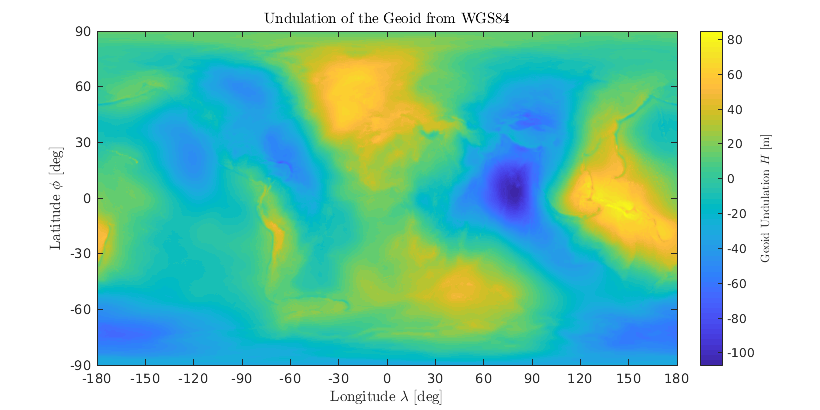
\includegraphics[width=\linewidth]{GeoidUndulationfromWGS84200Contours.png}
%	\begin{overpic}[width=\linewidth]{DisplacementofLocalTopographyfromtheGeoidBoneColorMapSeaLevelBlackkm.png}
%	\put(16.25,47.8){\colorbox{white}{Displacement of Local Topography from the Geoid (MSL)}} %20 w/o "(MSL)"
%	\put(38.5,0.55){\colorbox{white}{\small Longitude $\lambda$ [deg]}}
%%	\put(5, 18){\colorbox{white}{\rotatebox{90}{\small Latitude $\phi$ [deg]}}}
%	\put(5, 13.5){\colorbox{white}{\rotatebox{90}{\small Geodetic Latitude $\phi$ [deg]}}}
%	\put(93.5, 41.25){\colorbox{white}{\rotatebox{270}{\footnotesize Topography Displacement $H$ [m]}}}
%	
%	% Try overlaying ticks
%	% x axis
%	\put(9.7, 3.2){\colorbox{white}{\scriptsize -$180$}}
%	\put(15.55, 3.2){\colorbox{white}{\scriptsize -$150$}}
%	\put(21.6, 3.2){\colorbox{white}{\scriptsize -$120$}}
%	\put(28, 3.2){\colorbox{white}{\scriptsize -$90$}}
%	\put(34.2, 3.2){\colorbox{white}{\scriptsize -$60$}}
%	\put(40, 3.2){\colorbox{white}{\scriptsize -$30$}}
%	\put(47.1, 3.2){\colorbox{white}{\scriptsize $0$}}
%	\put(52.6, 3.2){\colorbox{white}{\scriptsize $30$}}
%	\put(58.6, 3.2){\colorbox{white}{\scriptsize $60$}}
%	\put(64.6, 3.2){\colorbox{white}{\scriptsize $90$}}
%	\put(70.2, 3.2){\colorbox{white}{\scriptsize $120$}}
%	\put(76.25, 3.2){\colorbox{white}{\scriptsize $150$}}
%	\put(81.8, 3.2){\colorbox{white}{\scriptsize $180$}}
%	
%	% y axis
%	\put(8.1, 5.45){\colorbox{white}{\scriptsize -$90$}}
%	\put(8.1, 11.75){\colorbox{white}{\scriptsize -$60$}}
%	\put(8.1, 18.7){\colorbox{white}{\scriptsize -$30$}}
%	\put(9.7, 25.6){\colorbox{white}{\scriptsize $0$}}
%	\put(8.8, 32.45){\colorbox{white}{\scriptsize $30$}}
%	\put(8.8, 39.4){\colorbox{white}{\scriptsize $60$}} % aligned
%	\put(8.8, 45.9){\colorbox{white}{\scriptsize $90$}}
%	
%	% z axis
%%	\put(88.3, 6.5){\colorbox{white}{\ssmall -$100$}} % 6.5
%	\put(88.3, 9.85){\colorbox{white}{\ssmall -$8000$}}
%	\put(88.3, 14.7){\colorbox{white}{\ssmall -$6000$}}
%	\put(88.3, 19.6){\colorbox{white}{\ssmall -$4000$}}
%	\put(88.3, 24.3){\colorbox{white}{\ssmall -$2000$}}
%	\put(88.3, 29.25){\colorbox{white}{\ssmall $0$}}
%	\put(88.3, 34.2){\colorbox{white}{\ssmall $2000$}}
%	\put(88.3, 39){\colorbox{white}{\ssmall $4000$}}
%	\put(88.3, 43.8){\colorbox{white}{\ssmall $6000$}}
%%	\put(88.3, 44.75){\colorbox{white}{\ssmall $8000$}}
%	\end{overpic}
%	\caption{The cylindrical projection of the variation of local surface topography from the tide-free geoid}
%	\label{fig:LocalTopographyDisplacementFromGeoid}
%\end{figure}

%~
%~
%~
%~
%~
%~
%~
%~
%~

%\begin{figure}[H]
%	\centering
%	\begin{overpic}[width=\linewidth]{DisplacementofLocalTopographyfromtheGeoidBoneColorMapSeaLevelBlack.png}
%	% Shown is such that H(H < -415) = NaN and NaN is set to black such that (0,0,0) is actually not on the color bar
%	% H(H < -415) = 0 would technically be more correct, but doesn't look as nice as 0 is a bit of grey
%	\put(14.25,46.9){\colorbox{white}{Displacement of Continental Topography from the Geoid (MSL)}} %20 w/o "(MSL)"
%	\put(38.5,0.55){\colorbox{white}{\small Longitude $\lambda$ [deg]}}
%%	\put(5, 18){\colorbox{white}{\rotatebox{90}{\small Latitude $\phi$ [deg]}}}
%	\put(5, 13.5){\colorbox{white}{\rotatebox{90}{\small Geodetic Latitude $\phi$ [deg]}}}
%	\put(92.8, 40.25){\colorbox{white}{\rotatebox{270}{\footnotesize Topography Displacement $H$ [m]}}}
%	
%	% Try overlaying ticks
%	% x axis
%	\put(9.7, 3.1){\colorbox{white}{\scriptsize -$180$}}
%	\put(15.5, 3.1){\colorbox{white}{\scriptsize -$150$}}
%	\put(21.4, 3.1){\colorbox{white}{\scriptsize -$120$}}
%	\put(28.1, 3.1){\colorbox{white}{\scriptsize -$90$}}
%	\put(34.2, 3.1){\colorbox{white}{\scriptsize -$60$}}
%	\put(40, 3.1){\colorbox{white}{\scriptsize -$30$}}
%	\put(47.15, 3.1){\colorbox{white}{\scriptsize $0$}}
%	\put(52.65, 3.1){\colorbox{white}{\scriptsize $30$}}
%	\put(58.65, 3.1){\colorbox{white}{\scriptsize $60$}}
%	\put(64.7, 3.1){\colorbox{white}{\scriptsize $90$}}
%	\put(70.2, 3.1){\colorbox{white}{\scriptsize $120$}}
%	\put(76.25, 3.1){\colorbox{white}{\scriptsize $150$}}
%	\put(81.8, 3.1){\colorbox{white}{\scriptsize $180$}}
%	
%	% y axis
%	\put(8.1, 5.45){\colorbox{white}{\scriptsize -$90$}}
%	\put(8.1, 11.4){\colorbox{white}{\scriptsize -$60$}}
%	\put(8.1, 18.2){\colorbox{white}{\scriptsize -$30$}}
%	\put(9.7, 24.85){\colorbox{white}{\scriptsize $0$}}
%	\put(8.8, 31.55){\colorbox{white}{\scriptsize $30$}}
%	\put(8.8, 38.2){\colorbox{white}{\scriptsize $60$}} % aligned
%	\put(8.8, 44.7){\colorbox{white}{\scriptsize $90$}}
%	
%	% z axis
%	\put(88.2, 7.1){\colorbox{white}{\ssmall $0$}} % 88.2
%	\put(88.2, 12.6){\colorbox{white}{\ssmall $1000$}}
%	\put(88.2, 18.0){\colorbox{white}{\ssmall $2000$}}
%	\put(88.2, 23.5){\colorbox{white}{\ssmall $3000$}}
%	\put(88.2, 28.8){\colorbox{white}{\ssmall $4000$}}
%	\put(88.2, 34.3){\colorbox{white}{\ssmall $5000$}}
%	\put(88.2, 39.7){\colorbox{white}{\ssmall $6000$}}
%	\end{overpic}
%	\caption{The variation of local surface topography on the continents from the tide-free geoid}
%	\label{fig:LocalTopographyDisplacementFromGeoidBlack}
%\end{figure}

%~
%~
%~
%~
%~
%~
%~
%~
%~

%\begin{figure}[H]
%	\centering
%	\begin{overpic}[width=\linewidth]{DisplacementofLocalTopographyfromtheGeoidBoneColorMapSeaLevelBlackWithGeoidUndulations.png}
%	% Shown is such that H(H < -415) = NaN and NaN is set to black such that (0,0,0) is actually not on the color bar
%	% H(H < -415) = 0 would technically be more correct, but doesn't look as nice as 0 is a bit of grey
%	\put(23.6,48.25){\colorbox{white}{Displacement of Earth's Surface from WGS84}} %20 w/o "(MSL)"
%	\put(38.5,0.55){\colorbox{white}{\small Longitude $\lambda$ [deg]}}
%%	\put(5, 18){\colorbox{white}{\rotatebox{90}{\small Latitude $\phi$ [deg]}}}
%	\put(5, 13.5){\colorbox{white}{\rotatebox{90}{\small Geodetic Latitude $\phi$ [deg]}}}
%	\put(92.8, 40.25){\colorbox{white}{\rotatebox{270}{\footnotesize Topography Displacement $H$ [m]}}}
%	
%	% Try overlaying ticks
%	% x axis
%	\put(9.7, 3.1){\colorbox{white}{\scriptsize -$180$}}
%	\put(15.5, 3.1){\colorbox{white}{\scriptsize -$150$}}
%	\put(21.4, 3.1){\colorbox{white}{\scriptsize -$120$}}
%	\put(28.1, 3.1){\colorbox{white}{\scriptsize -$90$}}
%	\put(34.2, 3.1){\colorbox{white}{\scriptsize -$60$}}
%	\put(40, 3.1){\colorbox{white}{\scriptsize -$30$}}
%	\put(47.15, 3.1){\colorbox{white}{\scriptsize $0$}}
%	\put(52.65, 3.1){\colorbox{white}{\scriptsize $30$}}
%	\put(58.65, 3.1){\colorbox{white}{\scriptsize $60$}}
%	\put(64.7, 3.1){\colorbox{white}{\scriptsize $90$}}
%	\put(70.2, 3.1){\colorbox{white}{\scriptsize $120$}}
%	\put(76.25, 3.1){\colorbox{white}{\scriptsize $150$}}
%	\put(81.8, 3.1){\colorbox{white}{\scriptsize $180$}}
%	
%	% y axis
%	\put(8.1, 5.65){\colorbox{white}{\scriptsize -$90$}}
%	\put(8.1, 11.8){\colorbox{white}{\scriptsize -$60$}}
%	\put(8.1, 18.6){\colorbox{white}{\scriptsize -$30$}}
%	\put(9.7, 25.5){\colorbox{white}{\scriptsize $0$}}
%	\put(8.8, 32.45){\colorbox{white}{\scriptsize $30$}}
%	\put(8.8, 39.2){\colorbox{white}{\scriptsize $60$}} % aligned
%	\put(8.8, 45.8){\colorbox{white}{\scriptsize $90$}}
%	
%	% z axis
%	\put(88.2, 7.9){\colorbox{white}{\ssmall $0$}} % 88.2
%	\put(88.2, 13.3){\colorbox{white}{\ssmall $1000$}}
%	\put(88.2, 18.9){\colorbox{white}{\ssmall $2000$}}
%	\put(88.2, 24.4){\colorbox{white}{\ssmall $3000$}}
%	\put(88.2, 29.9){\colorbox{white}{\ssmall $4000$}}
%	\put(88.2, 35.5){\colorbox{white}{\ssmall $5000$}}
%	\put(88.2, 40.9){\colorbox{white}{\ssmall $6000$}}
%	\end{overpic}
%	\caption{The variation of local surface topography on the continents from the tide-free geoid}
%	\label{fig:LocalTopographyDisplacementFromGeoidBlack}
%\end{figure}

%~
%~
%~
%~
%~
%~
%~
%~
%~

%\begin{table}[H]
%\centering
%\caption{EGM2008 tide-free, fully normalized, dimensionless harmonic coefficients $\overbar{C}_{nm}$ and $\overbar{S}_{nm}$ up to degree 5 and order 0. All zeroth order (zonal harmonic) terms $\overbar{S}_{n0}$ are unnecessary but written as zeros to eliminate any ambiguity. The set of harmonic coefficients in the zero-tide model is exactly the same as the tide-free set shown below except $\overbar{C}_{20} = -\num{0.484169317366974e-3}$ in the zero-tide model.}
%\begin{tabular}{c c S[scientific-notation=false, table-format=-1.15e-2] S[scientific-notation=false, table-format=-1.15e-2]} 
%\toprule
%{\specialcell{Degree \\ $n$}} & {\specialcell{Order \\ $m$}} & {\specialcell{Normalized Harmonic Coeff. \\ $\overbar{C}_{nm}$ (Dimensionless)}} & {\specialcell{Normalized Harmonic Coeff. \\ $\overbar{S}_{nm}$ (Dimensionless)}} \\ \midrule
%2  &  0  & -0.484165143790815D-03 &   0.000000000000000D+00 \\%    0.7481239490D-11    0.0000000000D+00
%   &  1  & -0.206615509074176D-09 &   0.138441389137979D-08 \\%    0.7063781502D-11    0.7348347201D-11
%   &  2  &  0.243938357328313D-05 &  -0.140027370385934D-05 \\%    0.7230231722D-11    0.7425816951D-11
%3  &  0  &  0.957161207093473D-06 &   0.000000000000000D+00 \\%    0.5731430751D-11    0.0000000000D+00
%   &  1  &  0.203046201047864D-05 &   0.248200415856872D-06 \\%    0.5726633183D-11    0.5976692146D-11
%   &  2  &  0.904787894809528D-06 &  -0.619005475177618D-06 \\%    0.6374776928D-11    0.6401837794D-11
%   &  3  &  0.721321757121568D-06 &   0.141434926192941D-05 \\%    0.6029131793D-11    0.6028311182D-11
%4  &  0  &  0.539965866638991D-06 &   0.000000000000000D+00 \\%    0.4431111968D-11    0.0000000000D+00
%   &  1  & -0.536157389388867D-06 &  -0.473567346518086D-06 \\%    0.4568074333D-11    0.4684043490D-11
%   &  2  &  0.350501623962649D-06 &   0.662480026275829D-06 \\%    0.5307840320D-11    0.5186098530D-11
%   &  3  &  0.990856766672321D-06 &  -0.200956723567452D-06 \\%    0.5631952953D-11    0.5620296098D-11
%   &  4  & -0.188519633023033D-06 &   0.308803882149194D-06 \\%    0.5372877167D-11    0.5383247677D-11
%5  &  0  &  0.686702913736681D-07 &   0.000000000000000D+00 \\%    0.2910198425D-11    0.0000000000D+00
%   &  1  & -0.629211923042529D-07 &  -0.943698073395769D-07 \\%    0.2989077566D-11    0.3143313186D-11
%   &  2  &  0.652078043176164D-06 &  -0.323353192540522D-06 \\%    0.3822796143D-11    0.3642768431D-11
%   &  3  & -0.451847152328843D-06 &  -0.214955408306046D-06 \\%    0.4725934077D-11    0.4688985442D-11
%   &  4  & -0.295328761175629D-06 &   0.498070550102351D-07 \\%    0.5332198489D-11    0.5302621028D-11
%   &  5  &  0.174811795496002D-06 &  -0.669379935180165D-06 \\%    0.4980396595D-11    0.4981027282D-11
%6  &  0  & -0.149953927978527D-06 &   0.000000000000000D+00 \\%    0.2035490195D-11    0.0000000000D+00
%   &  1  & -0.759210081892527D-07 &   0.265122593213647D-07 \\%    0.2085980159D-11    0.2193954647D-11
%   &  2  &  0.486488924604690D-07 &  -0.373789324523752D-06 \\%    0.2603949443D-11    0.2466506184D-11
%   &  3  &  0.572451611175653D-07 &   0.895201130010730D-08 \\%    0.3380286162D-11    0.3347204566D-11
%   &  4  & -0.860237937191611D-07 &  -0.471425573429095D-06 \\%    0.4535102219D-11    0.4489428324D-11
%   &  5  & -0.267166423703038D-06 &  -0.536493151500206D-06 \\%    0.5097794605D-11    0.5101153019D-11
%   &  6  &  0.947068749756882D-08 &  -0.237382353351005D-06 \\%    0.4731651005D-11    0.4728357086D-11
%7  &  0  &  0.905120844521618D-07 &   0.000000000000000D+00 \\%    0.1542363963D-11    0.0000000000D+00
%   &  1  &  0.280887555776673D-06 &   0.951259362869275D-07 \\%    0.1561721696D-11    0.1656779220D-11
%   &  2  &  0.330407993702235D-06 &   0.929969290624092D-07 \\%    0.1917954909D-11    0.1813082652D-11
%   &  3  &  0.250458409225729D-06 &  -0.217118287729610D-06 \\%    0.2421172504D-11    0.2406891912D-11
%   &  4  & -0.274993935591631D-06 &  -0.124058403514343D-06 \\%    0.3384737305D-11    0.3327030779D-11
%   &  5  &  0.164773255934658D-08 &   0.179281782751438D-07 \\%    0.4372616383D-11    0.4378544108D-11
%   &  6  & -0.358798423464889D-06 &   0.151798257443669D-06 \\%    0.5033507782D-11    0.5024794147D-11
%   &  7  &  0.150746472872675D-08 &   0.241068767286303D-07 \\%    0.4572229702D-11    0.4570746400D-11
%%8  &  0  &  0.494756003005199D-07 &   0.000000000000000D+00 \\%    0.1237051133D-11    0.0000000000D+00
%%   &  1  &  0.231607991248329D-07 &   0.588974540927606D-07 \\%    0.1241750465D-11    0.1326654814D-11
%%   &  2  &  0.800143604736599D-07 &   0.652805043667369D-07 \\%    0.1494951534D-11    0.1411005252D-11
%%   &  3  & -0.193745381715290D-07 &  -0.859639339125694D-07 \\%    0.1864101313D-11    0.1850301061D-11
%%   &  4  & -0.244360480007096D-06 &   0.698072508472777D-07 \\%    0.2597222975D-11    0.2556744174D-11
%%   &  5  & -0.257011477267991D-07 &   0.892034891745881D-07 \\%    0.3210497723D-11    0.3217620934D-11
%%   &  6  & -0.659648680031408D-07 &   0.308946730783065D-06 \\%    0.4312331128D-11    0.4296497239D-11
%%   &  7  &  0.672569751771483D-07 &   0.748686063738231D-07 \\%    0.4982969530D-11    0.4986624872D-11
%%   &  8  & -0.124022771917136D-06 &   0.120551889384997D-06 \\%    0.4498624439D-11    0.4501340997D-11
%%9  &  0  &  0.280180753216300D-07 &   0.000000000000000D+00 \\%    0.1023487582D-11    0.0000000000D+00
%%   &  1  &  0.142151377236084D-06 &   0.214004665077510D-07 \\%    0.1018511829D-11    0.1089176581D-11
%%   &  2  &  0.214144381199757D-07 &  -0.316984195352417D-07 \\%    0.1208927719D-11    0.1141907553D-11
%%   &  3  & -0.160612356882835D-06 &  -0.742658786809216D-07 \\%    0.1470083017D-11    0.1457047050D-11
%%   &  4  & -0.936529556592536D-08 &   0.199026740710063D-07 \\%    0.2110483299D-11    0.2073741397D-11
%%   &  5  & -0.163134050605937D-07 &  -0.540394840426217D-07 \\%    0.2551829532D-11    0.2558834844D-11
%%   &  6  &  0.627879491161446D-07 &   0.222962377434615D-06 \\%    0.3185143905D-11    0.3168799261D-11
%%   &  7  & -0.117983924385618D-06 &  -0.969222126840068D-07 \\%    0.4294900507D-11    0.4301792728D-11
%%   &  8  &  0.188136188986452D-06 &  -0.300538974811744D-08 \\%    0.5026516563D-11    0.5019526183D-11
%%   &  9  & -0.475568433357652D-07 &   0.968804214389955D-07 \\%    0.4457949868D-11    0.4455360399D-11
%%10 &  0  &  0.533304381729473D-07 &   0.000000000000000D+00 \\%    0.8818400481D-12    0.0000000000D+00
%\bottomrule
%\end{tabular}
%\end{table}
%
%\begin{table}[H]
%\centering
%\caption{EGM2008 fully normalized secular rates of the dimensionless harmonic coefficients $\overbar{C}_{nm}$ and $\overbar{S}_{nm}$ up to degree 2 and order 2.}
%\begin{tabular}{c c S[scientific-notation=false, table-format=-1.15e-2] S[scientific-notation=false, table-format=-1.15e-2]} 
%\toprule
%{\specialcell{Degree \\ $n$}} & {\specialcell{Order \\ $m$}} & {\specialcell{Normalized Secular Coeff. \\ $\dot{\overbar{C}}_{nm}$ ($1/\mathrm{yr}$)}} & {\specialcell{Normalized Secular Coeff. \\ $\dot{\overbar{S}}_{nm}$ ($1/\mathrm{yr}$)}} \\ \midrule
%2  &  0  & 1 & 1 \\
%2  &  1  & 1 & 1 \\
%%2  &  2  & 1 & 1 \\
%\bottomrule
%\end{tabular}
%\end{table}

%~
%~
%~
%~
%~
%~
%~
%~
%~

%\begin{table}[H]
%\centering
%\caption{The first few normalized FES2004 harmonic coefficients of wave modes modelling the effects of ocean tides on the gravitational coefficients. The full model is of degree and order 100 and does not include the atmospheric tide.}
%\label{tab:FES2004CnmpmbarhatSnmpmbarhat}
%\resizebox{\columnwidth}{!}{%
%\begin{tabular}{S[table-format=2]cc S[table-format=2.3] cccccccc}
%\toprule
%{\specialcell{D \\ $n$}} & {\specialcell{O \\ $m$}} & Tide & {\specialcell{Doodson \\ Number}}  &  $\overbar{\mathcal{S}}_{f,nm}^+$  &   $\overbar{\mathcal{C}}_{f,nm}^+$   &    $\overbar{\mathcal{S}}_{f,nm}^-$   &  $\overbar{\mathcal{C}}_{f,nm}^-$   &    $\hat{\overbar{\mathcal{C}}}_{f,nm}^+$  &  $\varepsilon_{f,nm}^+$   &    $\hat{\overbar{\mathcal{C}}}_{f,nm}^-$  &  $\varepsilon_{f,nm}^-$  \\ \midrule
%2  & 0 & Om1 &   55.565 & -0.540594 &   0.000000 &  0.000000 & 0.000000 &  0.5406 & 270.000 & 0.0000 &  0.000 \\
%2  & 0 & Om2 &   55.575 & -0.005218 &   0.000000 &  0.000000 & 0.000000 &  0.0052 & 270.000 & 0.0000 &  0.000 \\
%1  & 0 & Sa  &   56.554 &  0.017233 &   0.000013 &  0.000000 & 0.000000 &  0.0172 &  89.957 & 0.0000 &  0.000 \\
%2  & 0 & Sa  &   56.554 & -0.046604 &  -0.000903 &  0.000000 & 0.000000 &  0.0466 & 268.890 & 0.0000 &  0.000 \\
%3  & 0 & Sa  &   56.554 & -0.000889 &   0.000049 &  0.000000 & 0.000000 &  0.0009 & 273.155 & 0.0000 &  0.000 \\
%4  & 0 & Sa  &   56.554 &  0.012069 &  -0.000413 &  0.000000 & 0.000000 &  0.0121 &  91.960 & 0.0000 &  0.000 \\
%5  & 0 & Sa  &   56.554 & -0.009780 &  -0.000421 &  0.000000 & 0.000000 &  0.0098 & 267.535 & 0.0000 &  0.000 \\
%6  & 0 & Sa  &   56.554 &  0.006895 &   0.000043 &  0.000000 & 0.000000 &  0.0069 &  89.643 & 0.0000 &  0.000 \\
%7  & 0 & Sa  &   56.554 & -0.010515 &  -0.000287 &  0.000000 & 0.000000 &  0.0105 & 268.437 & 0.0000 &  0.000 \\
%8  & 0 & Sa  &   56.554 &  0.002067 &  -0.000011 &  0.000000 & 0.000000 &  0.0021 &  90.305 & 0.0000 &  0.000 \\
%9  & 0 & Sa  &   56.554 & -0.004236 &  -0.000110 &  0.000000 & 0.000000 &  0.0042 & 268.512 & 0.0000 &  0.000 \\
%10 & 0 & Sa  &   56.554 & -0.001781 &  -0.000085 &  0.000000 & 0.000000 &  0.0018 & 267.268 & 0.0000 &  0.000 \\
%%
%%56.554 Sa    1   1  0.000040  0.000035    0.000038  0.000056   0.0001  48.814 0.0001  34.160
%% 56.554 Sa    2   1 -0.000328 -0.000069   -0.000324  0.000124   0.0003 258.120 0.0003 290.943
%% 56.554 Sa    3   1  0.000476 -0.000228    0.000461  0.000259   0.0005 115.594 0.0005  60.672
%% 56.554 Sa    4   1 -0.000027 -0.000051   -0.000004  0.000053   0.0001 207.897 0.0001 355.684
%% 56.554 Sa    5   1  0.000485 -0.000334    0.000455  0.000381   0.0006 124.554 0.0006  50.058
%% 56.554 Sa    6   1 -0.000324  0.000211   -0.000305 -0.000234   0.0004 303.074 0.0004 232.504
%% 56.554 Sa    7   1  0.000047 -0.000494    0.000023  0.000499   0.0005 174.565 0.0005   2.639
%% 56.554 Sa    8   1  0.000304  0.000083    0.000287 -0.000128   0.0003  74.729 0.0003 114.037
%% 56.554 Sa    9   1 -0.000045 -0.000223   -0.000051  0.000231   0.0002 191.409 0.0002 347.550
%\bottomrule
%\end{tabular}
%}
%\end{table}

%~
%~
%~
%~
%~
%~
%~
%~
%~

%% The amount of occupied cross-sectional surface area then follows the quadratic relation
%\begin{equation}
%A_p(t) = \pi \left(r^2 - \big(r_{\hspace{-0.025em}p_0} + W(t)\big)^2\hspace{0.1em}\right).
%\end{equation}
% Reread and consider adding back in
% vvvv
%Of course, the location of the center of mass for the BATES grain will not change when considered as an isolated system.
%The center of mass obviously lies on the longitudinal axis for this grain, and following (\ref{eq:PropulsionCOMz}), the location of the center of mass from the bottom of the casing for times $t \in (0, t_b)$ is indeed constant when considered as an isolated system.
%\begin{align}
%\bar{z}_p(t) = \frac{1}{A_p(t) L_p} \int_0^{L_p} \iint_{A_p(t)} z\,dV = \frac{L_p}{2}.
%\end{align}
%Considering the propellant tube along with the rest of the rocket's body, however, causes considerable changes to the overall center of mass since the overall center of mass is the sum of contributions from all components.
%For $t \geqslant t_b$, however, this center of mass coordinate is no longer defined since, beginning at $t = t_b$, there physically is no more propellant.
%
%Suppose the (three-dimensional) body has a figure similar to that of Fig. \ref{fig:PropFuelRocket}, whereby the nose cone is elliptical and the body tube (the casing) is a cylinder. Also, let the fins and the nozzle be removed from consideration so that the vehicle ends with the propellant. Then the center of mass of the vehicle $\bar{z}$, with reference now along the longitudinal axis from the nosetip, is
%\begin{align}
%\bar{z}(t) &= \frac{m_n \bar{z}_n + m_b \bar{z}_b + m_p(t) \bar{z}_p}{m_n + m_b + m_p(t)}, \label{eq:PropulsionCOMSystem}
%\end{align}
%where $m_n$ and $\bar{z}_n$ are the nose cone mass and center of mass with respect to its tip, $m_b$ and $\bar{z}_b$ are body mass and center of the mass with respect to the nose cone's tip, and $m_p$ and $\bar{z}_p$ are the propellant's mass and center of mass at time $t$ with respect to the nose cone's tip. The propellant mass is consistent with
%\begin{equation}
%m_p(t) = m_p(0) + \int_0^t \dot{m}(s) \,ds,
%\end{equation}
%where $\dot{m}$ is inherently nonpositive. Note that even though $\bar{z}_p$ is undefined for $t \geqslant t_b$, (\ref{eq:PropulsionCOMSystem}) need not change since $m_p(t)$ has a nonnegative final value by physical intuition,
%\begin{equation}
%\lim_{t \to \infty} m_p(t) = 0.
%\end{equation}
%Actually, $m_p(t)$ has more than just a nonnegative final value; indeed $m_p(t) = 0$ for $t > t_b$. Note that the effect of tracking the center of mass from the nose tip is that staging a section simply removes it completely from consideration of (\ref{eq:PropulsionCOMSystem}).
%
%\section{Variation of the Inertia Tensor}
%
%
%%Suppose the propellant has an initial mass $M_0$ and occupies an initial volume $V_0 = L A_p(0)$ such that the average density throughout is $\rho = M_0/V_0$.

%~
%~
%~
%~
%~
%~
%~
%~
%~

%\begin{table}[H]
%\centering
%\caption{Reference atmosphere for temperature $T$ [\si{\K}] from $0$ to $90$ [\si{\km}] during the month of January.}
%\label{tab:ReferenceAtmosphere0to90kmJan}
%%\resizebox{\columnwidth}{!}{%
%\begin{tabular}{S[scientific-notation=false, table-format=2.3] | S[scientific-notation=false, table-format=3.2] S[scientific-notation=false, table-format=3.2] S[scientific-notation=false, table-format=3.2] S[scientific-notation=false, table-format=3.2] S[scientific-notation=false, table-format=3.2] S[scientific-notation=false, table-format=3.2] S[scientific-notation=false, table-format=3.2]}
%\toprule
%\multicolumn{8}{c}{January Temperature --- Reference Atmosphere at Geodetic Latitudes} \\ \midrule
%{\specialcell{Geom. Alt. \\ $h$ (\si{\km})}} & {$0^\circ$N} & {$15^\circ$N} & {$30^\circ$N} & {$45^\circ$N} & {$60^\circ$N} & {$75^\circ$N} & {$90^\circ$N} \\ \midrule
%0.000  & 299.15 & 296.65 & 287.15 & 272.15 & 257.15 & 248.15 & 237.15 \\ 
%2.000  & 288.78 & 287.27 & 281.16 & 265.15 & 255.94 & 251.37 & 245.88 \\
%4.000  & 278.41 & 277.90 & 268.20 & 255.66 & 248.73 & 240.36 & 236.61 \\
%6.000  & 268.06 & 266.28 & 255.24 & 243.68 & 234.13 & 229.35 & 226.60 \\
%8.000  & 256.40 & 252.35 & 242.28 & 231.71 & 220.54 & 218.35 & 216.59 \\ %\midrule
%10.000 & 240.49 & 238.42 & 229.36 & 219.74 & 217.15 & 214.14 & 212.64 \\
%12.000 & 224.58 & 224.50 & 216.40 & 218.65 & 217.15 & 212.14 & 210.64 \\
%14.000 & 208.69 & 210.59 & 211.08 & 217.66 & 217.15 & 210.14 & 208.63 \\
%16.000 & 197.34 & 199.46 & 205.91 & 216.67 & 216.66 & 208.15 & 204.64 \\
%18.000 & 195.03 & 195.15 & 203.15 & 215.67 & 215.66 & 206.16 & 200.65 \\ %\midrule
%20.000 & 201.37 & 203.65 & 207.71 & 215.15 & 214.66 & 204.16 & 196.67 \\
%22.000 & 207.71 & 212.59 & 212.49 & 215.15 & 213.67 & 202.93 & 196.65 \\ 
%24.000 & 214.05 & 217.22 & 217.25 & 215.15 & 212.68 & 204.12 & 196.65 \\
%26.000 & 220.38 & 221.58 & 221.79 & 215.15 & 212.98 & 205.32 & 196.65 \\
%28.000 & 226.71 & 225.93 & 225.36 & 217.08 & 214.77 & 206.51 & 196.65 \\ %\midrule
%30.000 & 232.70 & 230.28 & 228.92 & 221.44 & 216.55 & 209.00 & 203.04 \\
%32.000 & 236.65 & 234.63 & 233.13 & 225.79 & 218.34 & 212.97 & 209.59 \\ 
%34.000 & 240.60 & 238.97 & 237.67 & 230.15 & 220.12 & 216.94 & 216.14 \\
%36.000 & 244.55 & 244.29 & 242.24 & 235.54 & 222.07 & 220.90 & 222.69 \\
%38.000 & 249.66 & 250.20 & 246.98 & 241.47 & 224.25 & 224.86 & 229.23 \\ %\midrule
%40.000 & 254.98 & 256.12 & 251.71 & 247.40 & 226.43 & 228.82 & 232.98 \\
%42.000 & 260.30 & 262.02 & 256.45 & 253.32 & 232.87 & 232.78 & 236.55 \\
%44.000 & 265.61 & 265.70 & 261.17 & 259.24 & 239.78 & 236.74 & 240.11 \\
%46.000 & 270.92 & 268.84 & 265.65 & 262.82 & 245.16 & 240.69 & 243.67 \\
%48.000 & 272.15 & 271.15 & 265.65 & 264.65 & 247.93 & 244.64 & 247.22 \\ %\midrule
%50.000 & 272.15 & 271.15 & 265.65 & 264.65 & 250.69 & 248.59 & 250.79 \\
%52.000 & 269.12 & 268.95 & 261.73 & 261.41 & 251.15 & 252.53 & 252.15 \\
%54.000 & 265.01 & 264.43 & 256.62 & 255.51 & 251.15 & 255.15 & 252.15 \\
%56.000 & 260.71 & 259.92 & 251.65 & 250.83 & 250.93 & 254.06 \\
%58.000 & 255.61 & 254.49 & 247.13 & 247.29 & 250.54 & 250.71 \\ %\midrule
%60.000 & 250.52 & 249.01 & 242.62 & 243.76 & 250.11 & 247.39 \\
%62.000 & 245.44 & 243.53 & 238.12 & 240.22 & 245.59 & 244.03 \\
%64.000 & 240.35 & 238.05 & 233.61 & 236.69 & 241.08 & 240.69 \\
%66.000 & 235.27 & 232.58 & 229.11 & 233.17 & 238.65 & 238.52 \\
%68.000 & 230.19 & 226.62 & 224.62 & 229.64 & 238.65 & 240.09 \\ %\midrule
%70.000 & 225.12 & 228.57 & 220.12 & 226.12 & 238.65 & 241.66 \\
%72.000 & 217.25 & 214.88 & 218.15 & 225.65 & 238.07 & 239.43 \\
%74.000 & 206.72 & 210.20 & 218.15 & 225.65 & 234.16 & 235.52 \\
%76.000 & 196.20 & 205.53 & 216.35 & 223.44 & 230.25 & 231.60 \\
%78.000 & 195.65 & 200.85 & 212.84 & 219.54 & 226.34 & 227.69 \\ %\midrule 
%80.000 & 195.65 & 198.15 & 209.33 & 215.63 & 222.43 & 223.77 \\
%82.000 & 195.65 & 198.15 & 205.83 & 212.50 & 218.53 & 219.89 \\
%84.000 & 195.65 & 198.15 & 202.32 & 210.16 & 214.65 & 215.96 \\
%86.000 & 194.56 & 196.97 & 198.82 & 207.82 & 214.65 & 214.15 \\
%88.000 & 191.29 & 193.48 & 195.33 & 205.49 & 214.65 & 214.15 \\ %\midrule 
%90.000 & 187.99 & 189.99 & 191.83 & 203.15 & 214.65 & 214.15 \\ \bottomrule 
%\end{tabular}
%%}
%\end{table}%
%
%\begin{table}[H]
%\centering
%\caption{Reference atmosphere for temperature $T$ [\si{\K}] from $0$ to $90$ [\si{\km}] during the month of April.}
%\label{tab:ReferenceAtmosphere0to90kmApr}
%%\resizebox{\columnwidth}{!}{%
%\begin{tabular}{S[scientific-notation=false, table-format=2.3] | S[scientific-notation=false, table-format=3.2] S[scientific-notation=false, table-format=3.2] S[scientific-notation=false, table-format=3.2] S[scientific-notation=false, table-format=3.2] S[scientific-notation=false, table-format=3.2] S[scientific-notation=false, table-format=3.2] S[scientific-notation=false, table-format=3.2]}
%\toprule
%\multicolumn{8}{c}{April Temperature --- Reference Atmosphere at Geodetic Latitudes} \\ \midrule
%{\specialcell{Geom. Alt. \\ $h$ (\si{\km})}} & {$0^\circ$N} & {$15^\circ$N} & {$30^\circ$N} & {$45^\circ$N} & {$60^\circ$N} & {$75^\circ$N} & {$90^\circ$N} \\ \midrule
%0.000  & 300.15 & 297.15 & 292.15 & 279.15 & 269.15 & 255.15 & 248.65 \\
%2.000  & 288.98 & 286.97 & 282.16 & 273.15 & 263.14 & 254.88 & 252.12 \\
%4.000  & 277.82 & 276.81 & 272.19 & 263.66 & 257.13 & 244.86 & 242.11 \\
%6.000  & 266.67 & 264.78 & 260.24 & 250.68 & 243.13 & 233.85 & 232.10 \\
%8.000  & 254.63 & 250.85 & 246.29 & 237.71 & 229.14 & 222.85 & 222.09 \\
%10.000 & 239.71 & 236.92 & 232.35 & 224.75 & 222.15 & 222.56 & 221.91 \\
%12.000 & 224.81 & 223.00 & 218.42 & 218.15 & 222.15 & 224.15 & 224.15 \\
%14.000 & 209.91 & 209.09 & 213.47 & 218.15 & 222.15 & 224.15 & 224.15 \\
%16.000 & 198.56 & 200.02 & 208.69 & 218.15 & 222.15 & 224.15 & 224.15 \\
%18.000 & 196.12 & 196.15 & 206.15 & 218.15 & 222.15 & 224.15 & 224.15 \\
%20.000 & 202.66 & 204.84 & 210.92 & 218.15 & 222.15 & 224.15 & 224.15 \\
%22.000 & 209.20 & 213.96 & 215.88 & 218.15 & 222.15 & 224.15 & 224.15 \\
%24.000 & 215.74 & 221.02 & 220.46 & 220.26 & 222.15 & 224.15 & 224.66 \\
%26.000 & 222.27 & 225.38 & 225.02 & 223.24 & 223.17 & 224.15 & 226.85 \\
%28.000 & 228.39 & 229.73 & 229.57 & 226.21 & 225.35 & 224.15 & 229.04 \\
%30.000 & 233.93 & 234.08 & 234.13 & 229.54 & 227.53 & 227.61 & 231.23 \\
%32.000 & 239.46 & 238.43 & 238.68 & 234.49 & 231.97 & 231.97 & 233.41 \\
%34.000 & 244.98 & 242.77 & 243.05 & 239.44 & 236.53 & 234.76 & 236.16 \\
%36.000 & 250.51 & 247.24 & 247.39 & 244.54 & 241.59 & 238.33 & 241.12 \\
%38.000 & 256.03 & 252.77 & 251.73 & 250.47 & 247.33 & 241.89 & 246.08 \\
%40.000 & 261.54 & 258.28 & 256.07 & 256.40 & 253.07 & 248.03 & 251.03 \\
%42.000 & 267.06 & 263.80 & 260.41 & 261.09 & 258.80 & 254.36 & 255.98 \\
%44.000 & 269.72 & 268.24 & 263.77 & 265.04 & 264.53 & 260.69 & 260.93 \\
%46.000 & 271.69 & 270.21 & 266.92 & 268.08 & 269.24 & 267.02 & 265.87 \\
%48.000 & 272.15 & 272.15 & 269.15 & 271.65 & 272.20 & 273.34 & 270.15 \\
%50.000 & 272.15 & 272.15 & 269.15 & 271.65 & 274.15 & 274.15 & 270.15 \\
%52.000 & 269.27 & 269.52 & 267.98 & 269.06 & 274.15 & 274.15 & 270.15 \\
%54.000 & 265.35 & 265.99 & 263.46 & 264.34 & 270.80 & 272.01 & 270.15 \\
%56.000 & 261.42 & 261.78 & 258.95 & 259.62 & 264.90 & 265.91 \\
%58.000 & 256.93 & 254.72 & 253.74 & 254.31 & 259.00 & 259.41 \\
%60.000 & 249.49 & 247.67 & 248.25 & 249.01 & 253.10 & 253.11 \\
%62.000 & 242.05 & 240.62 & 242.76 & 243.71 & 247.21 & 246.82 \\
%64.000 & 234.62 & 233.58 & 237.28 & 238.42 & 241.31 & 240.53 \\
%66.000 & 227.20 & 226.54 & 231.80 & 233.13 & 236.24 & 234.24 \\
%68.000 & 219.76 & 219.51 & 226.20 & 229.09 & 232.12 & 230.47 \\
%70.000 & 211.95 & 212.48 & 220.53 & 225.53 & 228.01 & 226.75 \\
%72.000 & 204.15 & 205.86 & 214.87 & 221.26 & 223.90 & 223.02 \\
%74.000 & 196.35 & 199.63 & 209.21 & 217.35 & 219.79 & 219.30 \\
%76.000 & 188.55 & 193.39 & 203.55 & 213.44 & 215.33 & 215.58 \\
%78.000 & 190.73 & 193.15 & 200.17 & 209.54 & 210.25 & 209.96 \\
%80.000 & 193.45 & 193.15 & 199.20 & 205.63 & 205.17 & 204.09 \\
%82.000 & 196.40 & 195.44 & 198.22 & 201.11 & 200.09 & 198.23 \\
%84.000 & 199.70 & 197.97 & 197.25 & 196.13 & 195.02 & 192.37 \\
%86.000 & 203.00 & 200.49 & 196.28 & 191.27 & 189.95 & 186.51 \\
%88.000 & 206.30 & 203.02 & 195.31 & 189.65 & 184.88 & 180.66 \\
%90.000 & 209.60 & 205.54 & 194.34 & 189.65 & 179.81 & 176.15 \\ \bottomrule
%\end{tabular}
%%}
%\end{table}%

%~
%~
%~
%~
%~
%~
%~
%~
%~

%\begin{table}[H]
%\centering
%\caption{Reference atmosphere for temperature $T$ [\si{\K}] from $0$ to $90$ [\si{\km}] during the month of January.}
%\label{tab:ReferenceAtmosphere0to90kmJan}
%\resizebox{\columnwidth}{!}{%
%\begin{tabular}{c | c}
%\begin{tabular}{S[scientific-notation=false, table-format=2.3] | S[scientific-notation=false, table-format=3.2] S[scientific-notation=false, table-format=3.2] S[scientific-notation=false, table-format=3.2] S[scientific-notation=false, table-format=3.2] S[scientific-notation=false, table-format=3.2] S[scientific-notation=false, table-format=3.2] S[scientific-notation=false, table-format=3.2]}
%\toprule
%\multicolumn{8}{c}{January Temperature --- Reference Atmosphere at Geodetic Latitudes} \\ \midrule
%{\specialcell{$h$ (\si{\km})}} & {$0^\circ$N} & {$15^\circ$N} & {$30^\circ$N} & {$45^\circ$N} & {$60^\circ$N} & {$75^\circ$N} & {$90^\circ$N} \\ \midrule
%0.000  & 299.15 & 296.65 & 287.15 & 272.15 & 257.15 & 248.15 & 237.15 \\ 
%2.000  & 288.78 & 287.27 & 281.16 & 265.15 & 255.94 & 251.37 & 245.88 \\
%4.000  & 278.41 & 277.90 & 268.20 & 255.66 & 248.73 & 240.36 & 236.61 \\
%6.000  & 268.06 & 266.28 & 255.24 & 243.68 & 234.13 & 229.35 & 226.60 \\
%8.000  & 256.40 & 252.35 & 242.28 & 231.71 & 220.54 & 218.35 & 216.59 \\ %\midrule
%10.000 & 240.49 & 238.42 & 229.36 & 219.74 & 217.15 & 214.14 & 212.64 \\
%12.000 & 224.58 & 224.50 & 216.40 & 218.65 & 217.15 & 212.14 & 210.64 \\
%14.000 & 208.69 & 210.59 & 211.08 & 217.66 & 217.15 & 210.14 & 208.63 \\
%16.000 & 197.34 & 199.46 & 205.91 & 216.67 & 216.66 & 208.15 & 204.64 \\
%18.000 & 195.03 & 195.15 & 203.15 & 215.67 & 215.66 & 206.16 & 200.65 \\ %\midrule
%20.000 & 201.37 & 203.65 & 207.71 & 215.15 & 214.66 & 204.16 & 196.67 \\
%22.000 & 207.71 & 212.59 & 212.49 & 215.15 & 213.67 & 202.93 & 196.65 \\ 
%24.000 & 214.05 & 217.22 & 217.25 & 215.15 & 212.68 & 204.12 & 196.65 \\
%26.000 & 220.38 & 221.58 & 221.79 & 215.15 & 212.98 & 205.32 & 196.65 \\
%28.000 & 226.71 & 225.93 & 225.36 & 217.08 & 214.77 & 206.51 & 196.65 \\ %\midrule
%30.000 & 232.70 & 230.28 & 228.92 & 221.44 & 216.55 & 209.00 & 203.04 \\
%32.000 & 236.65 & 234.63 & 233.13 & 225.79 & 218.34 & 212.97 & 209.59 \\ 
%34.000 & 240.60 & 238.97 & 237.67 & 230.15 & 220.12 & 216.94 & 216.14 \\
%36.000 & 244.55 & 244.29 & 242.24 & 235.54 & 222.07 & 220.90 & 222.69 \\
%38.000 & 249.66 & 250.20 & 246.98 & 241.47 & 224.25 & 224.86 & 229.23 \\ %\midrule
%40.000 & 254.98 & 256.12 & 251.71 & 247.40 & 226.43 & 228.82 & 232.98 \\
%42.000 & 260.30 & 262.02 & 256.45 & 253.32 & 232.87 & 232.78 & 236.55 \\
%44.000 & 265.61 & 265.70 & 261.17 & 259.24 & 239.78 & 236.74 & 240.11 \\
%46.000 & 270.92 & 268.84 & 265.65 & 262.82 & 245.16 & 240.69 & 243.67 \\
%48.000 & 272.15 & 271.15 & 265.65 & 264.65 & 247.93 & 244.64 & 247.22 \\ %\midrule
%50.000 & 272.15 & 271.15 & 265.65 & 264.65 & 250.69 & 248.59 & 250.79 \\
%52.000 & 269.12 & 268.95 & 261.73 & 261.41 & 251.15 & 252.53 & 252.15 \\
%54.000 & 265.01 & 264.43 & 256.62 & 255.51 & 251.15 & 255.15 & 252.15 \\
%56.000 & 260.71 & 259.92 & 251.65 & 250.83 & 250.93 & 254.06 \\
%58.000 & 255.61 & 254.49 & 247.13 & 247.29 & 250.54 & 250.71 \\ %\midrule
%60.000 & 250.52 & 249.01 & 242.62 & 243.76 & 250.11 & 247.39 \\
%62.000 & 245.44 & 243.53 & 238.12 & 240.22 & 245.59 & 244.03 \\
%64.000 & 240.35 & 238.05 & 233.61 & 236.69 & 241.08 & 240.69 \\
%66.000 & 235.27 & 232.58 & 229.11 & 233.17 & 238.65 & 238.52 \\
%68.000 & 230.19 & 226.62 & 224.62 & 229.64 & 238.65 & 240.09 \\ %\midrule
%70.000 & 225.12 & 228.57 & 220.12 & 226.12 & 238.65 & 241.66 \\
%72.000 & 217.25 & 214.88 & 218.15 & 225.65 & 238.07 & 239.43 \\
%74.000 & 206.72 & 210.20 & 218.15 & 225.65 & 234.16 & 235.52 \\
%76.000 & 196.20 & 205.53 & 216.35 & 223.44 & 230.25 & 231.60 \\
%78.000 & 195.65 & 200.85 & 212.84 & 219.54 & 226.34 & 227.69 \\ %\midrule 
%80.000 & 195.65 & 198.15 & 209.33 & 215.63 & 222.43 & 223.77 \\
%82.000 & 195.65 & 198.15 & 205.83 & 212.50 & 218.53 & 219.89 \\
%84.000 & 195.65 & 198.15 & 202.32 & 210.16 & 214.65 & 215.96 \\
%86.000 & 194.56 & 196.97 & 198.82 & 207.82 & 214.65 & 214.15 \\
%88.000 & 191.29 & 193.48 & 195.33 & 205.49 & 214.65 & 214.15 \\ %\midrule 
%90.000 & 187.99 & 189.99 & 191.83 & 203.15 & 214.65 & 214.15 \\ \bottomrule 
%\end{tabular}
%&
%\begin{tabular}{S[scientific-notation=false, table-format=2.3] | S[scientific-notation=false, table-format=3.2] S[scientific-notation=false, table-format=3.2] S[scientific-notation=false, table-format=3.2] S[scientific-notation=false, table-format=3.2] S[scientific-notation=false, table-format=3.2] S[scientific-notation=false, table-format=3.2] S[scientific-notation=false, table-format=3.2]}
%\toprule
%\multicolumn{8}{c}{April Temperature --- Reference Atmosphere at Geodetic Latitudes} \\ \midrule
%{\specialcell{$h$ (\si{\km})}} & {$0^\circ$N} & {$15^\circ$N} & {$30^\circ$N} & {$45^\circ$N} & {$60^\circ$N} & {$75^\circ$N} & {$90^\circ$N} \\ \midrule
%0.000  & 300.15 & 297.15 & 292.15 & 279.15 & 269.15 & 255.15 & 248.65 \\
%2.000  & 288.98 & 286.97 & 282.16 & 273.15 & 263.14 & 254.88 & 252.12 \\
%4.000  & 277.82 & 276.81 & 272.19 & 263.66 & 257.13 & 244.86 & 242.11 \\
%6.000  & 266.67 & 264.78 & 260.24 & 250.68 & 243.13 & 233.85 & 232.10 \\
%8.000  & 254.63 & 250.85 & 246.29 & 237.71 & 229.14 & 222.85 & 222.09 \\
%10.000 & 239.71 & 236.92 & 232.35 & 224.75 & 222.15 & 222.56 & 221.91 \\
%12.000 & 224.81 & 223.00 & 218.42 & 218.15 & 222.15 & 224.15 & 224.15 \\
%14.000 & 209.91 & 209.09 & 213.47 & 218.15 & 222.15 & 224.15 & 224.15 \\
%16.000 & 198.56 & 200.02 & 208.69 & 218.15 & 222.15 & 224.15 & 224.15 \\
%18.000 & 196.12 & 196.15 & 206.15 & 218.15 & 222.15 & 224.15 & 224.15 \\
%20.000 & 202.66 & 204.84 & 210.92 & 218.15 & 222.15 & 224.15 & 224.15 \\
%22.000 & 209.20 & 213.96 & 215.88 & 218.15 & 222.15 & 224.15 & 224.15 \\
%24.000 & 215.74 & 221.02 & 220.46 & 220.26 & 222.15 & 224.15 & 224.66 \\
%26.000 & 222.27 & 225.38 & 225.02 & 223.24 & 223.17 & 224.15 & 226.85 \\
%28.000 & 228.39 & 229.73 & 229.57 & 226.21 & 225.35 & 224.15 & 229.04 \\
%30.000 & 233.93 & 234.08 & 234.13 & 229.54 & 227.53 & 227.61 & 231.23 \\
%32.000 & 239.46 & 238.43 & 238.68 & 234.49 & 231.97 & 231.97 & 233.41 \\
%34.000 & 244.98 & 242.77 & 243.05 & 239.44 & 236.53 & 234.76 & 236.16 \\
%36.000 & 250.51 & 247.24 & 247.39 & 244.54 & 241.59 & 238.33 & 241.12 \\
%38.000 & 256.03 & 252.77 & 251.73 & 250.47 & 247.33 & 241.89 & 246.08 \\
%40.000 & 261.54 & 258.28 & 256.07 & 256.40 & 253.07 & 248.03 & 251.03 \\
%42.000 & 267.06 & 263.80 & 260.41 & 261.09 & 258.80 & 254.36 & 255.98 \\
%44.000 & 269.72 & 268.24 & 263.77 & 265.04 & 264.53 & 260.69 & 260.93 \\
%46.000 & 271.69 & 270.21 & 266.92 & 268.08 & 269.24 & 267.02 & 265.87 \\
%48.000 & 272.15 & 272.15 & 269.15 & 271.65 & 272.20 & 273.34 & 270.15 \\
%50.000 & 272.15 & 272.15 & 269.15 & 271.65 & 274.15 & 274.15 & 270.15 \\
%52.000 & 269.27 & 269.52 & 267.98 & 269.06 & 274.15 & 274.15 & 270.15 \\
%54.000 & 265.35 & 265.99 & 263.46 & 264.34 & 270.80 & 272.01 & 270.15 \\
%56.000 & 261.42 & 261.78 & 258.95 & 259.62 & 264.90 & 265.91 \\
%58.000 & 256.93 & 254.72 & 253.74 & 254.31 & 259.00 & 259.41 \\
%60.000 & 249.49 & 247.67 & 248.25 & 249.01 & 253.10 & 253.11 \\
%62.000 & 242.05 & 240.62 & 242.76 & 243.71 & 247.21 & 246.82 \\
%64.000 & 234.62 & 233.58 & 237.28 & 238.42 & 241.31 & 240.53 \\
%66.000 & 227.20 & 226.54 & 231.80 & 233.13 & 236.24 & 234.24 \\
%68.000 & 219.76 & 219.51 & 226.20 & 229.09 & 232.12 & 230.47 \\
%70.000 & 211.95 & 212.48 & 220.53 & 225.53 & 228.01 & 226.75 \\
%72.000 & 204.15 & 205.86 & 214.87 & 221.26 & 223.90 & 223.02 \\
%74.000 & 196.35 & 199.63 & 209.21 & 217.35 & 219.79 & 219.30 \\
%76.000 & 188.55 & 193.39 & 203.55 & 213.44 & 215.33 & 215.58 \\
%78.000 & 190.73 & 193.15 & 200.17 & 209.54 & 210.25 & 209.96 \\
%80.000 & 193.45 & 193.15 & 199.20 & 205.63 & 205.17 & 204.09 \\
%82.000 & 196.40 & 195.44 & 198.22 & 201.11 & 200.09 & 198.23 \\
%84.000 & 199.70 & 197.97 & 197.25 & 196.13 & 195.02 & 192.37 \\
%86.000 & 203.00 & 200.49 & 196.28 & 191.27 & 189.95 & 186.51 \\
%88.000 & 206.30 & 203.02 & 195.31 & 189.65 & 184.88 & 180.66 \\
%90.000 & 209.60 & 205.54 & 194.34 & 189.65 & 179.81 & 176.15 \\ \bottomrule
%\end{tabular}
%\end{tabular}
%}
%\end{table}%

%~
%~
%~
%~
%~
%~
%~
%~
%~

%A rocket, whether intended for purely atmospheric flight or insertion into orbit, launches from a nearly upright position, held in place only by the \textit{launch tower}, which, depending on the size of the rocket, may or may not be situated on a \textit{launch pad}. For smaller rockets, the launch tower might resemble a (straight) rod (on the order of several meters long) called the \textit{guide rail} along which the rocket slides upon motor ignition.
%
%Before liftoff occurs, however, the rocket is statically situated in a nearly upright position. As such, the rocket is held in place by the launch pad (or ground) \textit{and} the tower in general. Suppose the rocket is of mass $m$ and the gravity model $g$ is (\ref{eq:LocalGravity}), (\ref{eq:SpheroidGravityAth}), or (\ref{eq:GravitationalAccelSPHR}). Further suppose that the rocket rests on the guide rail which is offset from the local direction of gravity by an angle $\delta$, and offset from the ENV basis component $\widehat{E}$ by the positive (counterclockwise) angle $\psi$ about the $\widehat{V}$ element. The frame created by this 3-rotation is the \textit{firing frame} defined by basis elements $\{\hat{1}, \hat{2}, \hat{3}\}$ which are related to the ENV elements $\{\widehat{E}, \widehat{N}, \widehat{V}\}$ via
%\begin{equation}
%\begin{pmatrix}x_1 \\ x_2 \\ x_3\end{pmatrix} = \underbrace{\begin{pmatrix}\cos\psi & \sin\psi & 0 \\ -\sin\psi & \cos\psi & 0 \\ 0 & 0 & 1\end{pmatrix}}_{\mathbf{T}^{\text{loc}/\text{env}}} \begin{pmatrix}\lambda' \\ \phi' \\ h'\end{pmatrix}
%\end{equation}
%
%If the reactionary forces on the rail are taken such that $F_N$ is normal to the rail and $F_P$ is parallel to the rail, then
%\begin{align}
%F_P = mg \cos\delta && F_N = mg \sin\delta.
%\end{align}
%The force $F_P$ may not be necessarily held entirely by the guide rail, but $F_N$ is. These forces dominate while the rocket is on the ground without producing any thrust such that \textit{the total acceleration is nothing}.
%
%Defining a new coordinate frame relative to the ENV frame by a simple positive (counterclockwise) rotation $\psi$ about the $\widehat{V}$ axis
%
%
%\section{Rail-Guided Flight}
%Supposing the motor is of sufficient size to provide an amount of thrust exceeding the rocket's weight, the rocket begins to move along the rail guide after the motor ignition. During this time, the rocket's flight path is a straight line regardless of the launch rail's orientation with respect to the local direction of gravity. For rockets incapable of thrust vectoring, this orientation largely determines the \textit{downrange direction}, i.e. ``where the rocket is going.'' With this idea in mind, let $\psi$
%
%With this in mind, let $t_0$ be the initial local time of motor ignition
%
%Consequently, the equations of motion in the 



















% !!!!!!!!!!!!!!!~!!!!!!!!!!!!!!!!!!!
% Graveyard of TikZ
% !!!!!!!!!!!!!!!~!!!!!!!!!!!!!!!!!!!
%~
%~
% !!!!!!!!!!!!!!!~!!!!!!!!!!!!!!!!!!!
% Colored Ellipsoid in r
% !!!!!!!!!!!!!!!~!!!!!!!!!!!!!!!!!!!
%% square of the half axes
%\newcommand{\asa}{1}
%\newcommand{\bsa}{1}
%\newcommand{\csa}{0.7}
%% view angle
%\tdplotsetmaincoords{70}{135}
%%
%\begin{tikzpicture}[scale=2,tdplot_main_coords,line join=bevel,fill opacity=.8]
%    \pgfsetlinewidth{.1pt}
%    \tdplotsphericalsurfaceplot[parametricfill]{72}{36}%
%        {1/sqrt((sin(\tdplottheta))^2*(cos(\tdplotphi))^2/\asa+
%        (sin(\tdplottheta))^2*(sin(\tdplotphi))^2/\bsa + (cos(\tdplottheta))^2/\csa)} % function defining radius
%        {black} % line color
%        {2*\tdplottheta} % fill
%        {\draw[color=black,thick,->] (0,0,0) -- (2,0,0) node[anchor=north east]{$x$};}% x-axis
%       {\draw[color=black,thick,->] (0,0,0) -- (0,1.5,0) node[anchor=north west]{$y$};}% y-axis
%        {\draw[color=black,thick,->] (0,0,0) -- (0,0,1) node[anchor=south]{$z$};}% z-axis
%\end{tikzpicture}
%~
%~
% !!!!!!!!!!!!!!!~!!!!!!!!!!!!!!!!!!!
% J2000 ECI and J2000 ECEF bases - the view is slightly scuffed just enough to matter and have to start over
% !!!!!!!!!!!!!!!~!!!!!!!!!!!!!!!!!!!
%\begin{figure}
%\centering
%%\tdplotsetmaincoords{70}{110} Use this in the future with [tdplot_main_coords]
%\begin{tikzpicture}[scale=4]
%% Set viewing angle (?) Not sure if this does anything
%\tdplotsetrotatedcoords{0}{0}{-9}
%
%% Set rotation angles for 213 sequence
%\pgfmathsetmacro{\phiOne}{0} % | 0
%\pgfmathsetmacro{\phiTwo}{30} % | 45
%\pgfmathsetmacro{\phiThree}{0} % | 0
%
%% Set resulting basis components
%\pgfmathsetmacro{\eOneOne}{cos(\phiTwo)*cos(\phiThree)}
%\pgfmathsetmacro{\eOneTwo}{sin(\phiThree)}
%\pgfmathsetmacro{\eOneThree}{-cos(\phiThree)*sin(\phiTwo)}
%%
%\pgfmathsetmacro{\eTwoOne}{sin(\phiOne)*sin(\phiTwo) - cos(\phiOne)*cos(\phiTwo)*sin(\phiThree)}
%\pgfmathsetmacro{\eTwoTwo}{cos(\phiOne)*cos(\phiThree)}
%\pgfmathsetmacro{\eTwoThree}{cos(\phiTwo)*sin(\phiOne) + cos(\phiOne)*sin(\phiTwo)*sin(\phiThree)}
%%
%\pgfmathsetmacro{\eThreeOne}{cos(\phiOne)*sin(\phiTwo) + cos(\phiTwo)*sin(\phiOne)*sin(\phiThree)}
%\pgfmathsetmacro{\eThreeTwo}{-cos(\phiThree)*sin(\phiOne)}
%\pgfmathsetmacro{\eThreeThree}{cos(\phiOne)*cos(\phiTwo) - sin(\phiOne)*sin(\phiTwo)*sin(\phiThree)}
%
%% Set position for object X
%\pgfmathsetmacro{\XOne}{0.9} % | 0.34
%\pgfmathsetmacro{\XTwo}{0.93} % | 0.6
%\pgfmathsetmacro{\XThree}{0.46} % | 0.9
%
%% Draw grid in the XY plane
%\begin{scope}[canvas is xz plane at y=0]
%\fill[black!15,opacity=0.25] circle [radius=1.2];
%\clip[draw] circle [radius=1.2];
%\draw[black!25,thin] [step=0.2] (-10,-10) grid (10,10);
%\end{scope}
%\pgfmathsetmacro{\Pd}{1.2}
%\pgfmathsetmacro{\Ld}{1*\Pd}
%%\fill[black!15,opacity=0.25] (\Pd,0,\Pd) -- (\Pd,0,-\Pd) -- (-\Pd+0.2,0,-\Pd) -- (-\Pd+0.2,0,\Pd) -- cycle;
%%\foreach \x in {-1,-0.8,...,1} {
%%  \ifthenelse{\NOT -1 = \x}{\draw[black!25,thin] (\x,0,-\Ld) -- (\x,0,\Ld);}{}
%%  \draw[black!25,thin] (-\Ld+0.2,0,\x) -- (\Ld,0,\x);
%%}
%
%% Create coordinates for object X
%\coordinate (X) at (\XOne,\XTwo,\XThree);
%
%% Draw axes
%\draw[->, >=latex, thick] (0,0,0) -- (1,0,0) node[right]{$\hat{\jmath}$}; % y
%\draw[->, >=latex, thick] (0,0,0) -- (0,1,0) node[below left]{$\hat{k}$}; % z
%\draw[->, >=latex, thick] (0,0,0) -- (0,0,1) node[left]{$\hat{\imath}$} node[right]{\ \vernal}; % x
%%
%\draw[->, >=latex, thick] (0,0,0) -- (\eOneOne,\eOneTwo,\eOneThree) node[right]{$\hat{J}$};
%\draw[->, >=latex, thick] (0,0,0) -- (\eTwoOne,\eTwoTwo,\eTwoThree) node[below right]{$\hat{K}$};
%\draw[->, >=latex, thick] (0,0,0) -- (\eThreeOne,\eThreeTwo,\eThreeThree) node[right]{$\hat{I}$};
%
%% Draw object X
%\draw (X) node[circle, fill, inner sep=1]{} node[above, left]{$\mathfrak{X}$};
%
%%% Add dashed vertical lines of rotated axes to the XY plane
%%\draw[dashed] (\eOneOne,0,\eOneThree) -- (\eOneOne,\eOneTwo,\eOneThree);
%%\draw[dashed] (\eTwoOne,0,\eTwoThree) -- (\eTwoOne,\eTwoTwo,\eTwoThree);
%%\draw[dashed] (\eThreeOne,0,\eThreeThree) -- (\eThreeOne,\eThreeTwo,\eThreeThree);
%
%% Add dashed lines from X to the XY plane
%\draw[dashed] (\XOne,0,\XThree) -- (\XOne,\XTwo,\XThree) node[pos=0.8, left]{$z$};
%%\draw[dashed] (0,0,0) -- (\XOne, 0, \XThree);
%\draw[dashed] (\XOne, 0, \XThree) -- (0, 0, \XThree) node[midway, above]{$y$};
%\draw[dashed] (\XOne, 0, \XThree) -- (\XOne, 0, 0) node[midway, right]{$x$};
%
%% Add dashed lines from X to the q2q3 plane
%% ~
%% Define its coordinate
%\coordinate (XProj) at (\XOne, 0, \XThree);
%
%\pgfmathsetmacro{\ECEFOne}{\XThree*cos(\phiTwo)+\XOne*sin(\phiTwo)};
%\pgfmathsetmacro{\ECEFThree}{-\XThree*sin(\phiTwo)+\XOne*cos(\phiTwo)};
%% Draw
%\draw[dashed] (XProj) -- (\XOne, \XTwo, \XThree) node[pos=0.8, right]{$Z$};
%\draw[dashed] (XProj) -- (\ECEFOne*\eThreeOne, 0, \ECEFOne*\eThreeThree) node[pos=0.5, below]{$Y$};
%\draw[dashed] (XProj) -- (\ECEFThree*\eOneOne, 0, \ECEFThree*\eOneThree) node[pos=0.3, left]{$X$};
%
%
%% Add labels to XY plane and R3
%\node[cm={1,0,cos(35),sin(55),(0,0)}] at ({(-0.71+0.15)*\Pd},0,{(0.58-0.16)*\Pd}){J2000};
%\node[cm={1,0,cos(35),sin(55),(0,0)}] at ({(-0.51+0.05)*\Pd},0,{(0.76-0.16)*\Pd}){Equatorial Plane}; % | -0.51 and 0.76
%
%% Draw angle arc between i and I axis (3-axis)
%\tdplotdrawarc[->,tdplot_rotated_coords]{(0,0,0)}{0.72}{0}{\phiTwo-1.6}{anchor=north}{$\lambda_G$}
%
%% Try to draw a (spherical) Earth at origin
%\shade[ball color=blue!40, opacity=0.4](0,0) circle (0.15);
%\end{tikzpicture}
%\caption{An object $W$ is shown to exist and be expressed in the J2000 (stationary basis $\{\hat{\imath}, \hat{\jmath}, \hat{k}\}$) and ECEF (rotating basis $\{\hat{I}, \hat{J}, \hat{K}\}$) coordinate systems.}
%\end{figure}
%~
%~
% !!!!!!!!!!!!!!!~!!!!!!!!!!!!!!!!!!!
% (failure) J2000 ECEF and SPHR bases - Couldn't figure out how to get 3d projections of both sphere and axes
% !!!!!!!!!!!!!!!~!!!!!!!!!!!!!!!!!!!
%\begin{figure}[H]
%\centering
%\pgfmathsetmacro{\viewO}{60}
%\pgfmathsetmacro{\viewT}{110}
%\tdplotsetmaincoords{\viewO}{\viewT} % 50, 135  |  60, 75 gives the same view of ECEF wrt ECI
%%
%\pgfmathsetmacro{\rvec}{.4}
%\pgfmathsetmacro{\thetavec}{30}
%\pgfmathsetmacro{\phivec}{60}
%%
%\begin{tikzpicture}[tdplot_main_coords, scale=4]
%\begin{scope}[canvas is yz plane at x=0]
%\pgfmathsetmacro{\R}{0.5} % sphere radius
%\pgfmathsetmacro{\angEl}{35} % elevation angle
%\draw (0,0) circle (\R);
%\foreach \t in {-80,-70,...,80} { \DrawLatitudeCircle[\R]{\t} }
%\foreach \t in {-5,-20,...,-180} { \DrawLongitudeCircle[\R]{\t} }
%\end{scope}
%
%% Draw coordinate grid in xy plane
%\pgfmathsetmacro{\Pd}{1.2}
%\pgfmathsetmacro{\Ld}{1*\Pd}
%\foreach \x in {-1,-0.8,...,1} {
%  \ifthenelse{\NOT -1 = \x}{\draw[black!25,thin] (\x,-\Ld,0) -- (\x,\Ld,0);}{}
%  \draw[black!25,thin] (-\Ld+0.2,\x,0) -- (\Ld,\x,0);
%}
%
%\draw[->, >=latex, thick] (0,0,0) -- (1,0,0) node[right]{$\hat{\imath}$};
%\draw[->, >=latex, thick] (0,0,0) -- (0,1,0) node[anchor=bottom, right]{$\hat{\jmath}$};
%\draw[->, >=latex, thick] (0,0,0) -- (0,0,1) node[anchor=north west]{$\hat{k}$};
%\tdplotsetcoord{P}{\rvec}{\thetavec}{\phivec}
%\draw[-stealth,color=red] (0,0,0) -- (P);
%\draw[dashed, color=red] (0,0,0) -- (Pxy);
%\draw[dashed, color=red] (P) -- (Pxy);
%\tdplotdrawarc[->,>=stealth]{(0,0,0)}{0.2}{0}{\phivec}{anchor=north}{$\lambda$}
%\tdplotsetthetaplanecoords{\phivec}
%\tdplotdrawarc[->,>=stealth, tdplot_rotated_coords]{(0,0,0)}{0.5}{0}{\thetavec}{anchor=south west}{$\theta$}
%\draw[dashed,tdplot_rotated_coords] (\rvec,0,0) arc (0:90:\rvec);
%\draw[dashed] (\rvec,0,0) arc (0:90:\rvec);
%\tdplotsetrotatedcoords{\phivec}{\thetavec}{0}
%\tdplotsetrotatedcoordsorigin{(P)}
%\draw[thick,tdplot_rotated_coords,->] (0,0,0) -- (.5,0,0) node[anchor=north west]{$x'$};
%\draw[thick,tdplot_rotated_coords,->] (0,0,0) -- (0,.5,0) node[anchor=west]{$y'$};
%\draw[thick,tdplot_rotated_coords,->] (0,0,0) -- (0,0,.5) node[anchor=south]{$z'$};
%\draw[-stealth,color=blue,tdplot_rotated_coords] (0,0,0) -- (.2,.2,.2);
%\draw[dashed,color=blue,tdplot_rotated_coords] (0,0,0) -- (.2,.2,0);
%\draw[dashed,color=blue,tdplot_rotated_coords] (.2,.2,0) -- (.2,.2,.2);
%\tdplotdrawarc[tdplot_rotated_coords,color=blue]{(0,0,0)}{0.2}{0}{45}{anchor=north west,color=black}{$\phi'$}
%\tdplotsetrotatedthetaplanecoords{45}
%\tdplotdrawarc[tdplot_rotated_coords,color=blue]{(0,0,0)}{0.2}{0}{55}{anchor=south west,color=black}{$\theta'$}
%\end{tikzpicture}
%\end{figure}




%~
%~
% !!!!!!!!!!!!!!!~!!!!!!!!!!!!!!!!!!!
% Physics vs Math SPHR coords. - Didn't like - settled on words
% !!!!!!!!!!!!!!!~!!!!!!!!!!!!!!!!!!!
%\begin{center}
%\tdplotsetmaincoords{70}{110}
%\pgfmathsetmacro{\ax}{0.5}
%\pgfmathsetmacro{\ay}{0.85}
%\pgfmathsetmacro{\az}{1}
%\pgfmathsetmacro{\r}{sqrt(\ax*\ax + \ay*\ay + \az*\az)}
%\pgfmathsetmacro{\SPHRtheta}{acos(\az/\r)}
%\pgfmathsetmacro{\SPHRlambda}{atan(\ay/\ax)}
%\begin{tikzpicture}[scale=4,tdplot_main_coords]
%\draw[->, >=latex, thick] (0,0,0) -- (1,0,0) node[anchor=west, xshift=1.5mm, yshift=-0.75mm]{$\hat{e}_\xi$};
%\draw[->, >=latex, thick] (0,0,0) -- (0,1,0) node[anchor=west]{$\hat{e}_\eta$};
%\draw[->, >=latex, thick] (0,0,0) -- (0,0,1) node[right]{$\hat{e}_\zeta$};
%\draw[dashed] (0,0,0) -- (\ax,\ay,\az) node[pos=0.6,above]{$r$} node[right]{$\mathfrak{X}$};
%\draw[] (\ax,\ay,\az) node[circle, fill, inner sep=1]{};
%\draw[loosely dashed] (0,0,0) -- (\ax,\ay,0);
%\draw[dashed] (\ax,\ay,0) -- (\ax,\ay,\az);
%\tdplotdrawarc[->,>=stealth]{(0,0,0)}{0.45}{0}{\SPHRlambda}{below}{$\phi$}
%\tdplotgetpolarcoords{\ax}{\ay}{\az}
%\tdplotsetthetaplanecoords{\tdplotresphi}
%\tdplotdrawarc[->,>=stealth,tdplot_rotated_coords]{(0,0,0)}{0.5}{0}{\tdplotrestheta}{anchor=west}{$\theta$}
%\end{tikzpicture}
%\hspace{20ex}
%\begin{tikzpicture}[scale=4,tdplot_main_coords]
%\draw[->, >=latex, thick] (0,0,0) -- (1,0,0) node[anchor=west, xshift=1.5mm, yshift=-0.75mm]{$\hat{e}_\xi$};
%\draw[->, >=latex, thick] (0,0,0) -- (0,1,0) node[anchor=west]{$\hat{e}_\eta$};
%\draw[->, >=latex, thick] (0,0,0) -- (0,0,1) node[right]{$\hat{e}_\zeta$};
%\draw[dashed] (0,0,0) -- (\ax,\ay,\az) node[pos=0.6,above]{$r$} node[right]{$\mathfrak{X}$};
%\draw[] (\ax,\ay,\az) node[circle, fill, inner sep=1]{};
%\draw[loosely dashed] (0,0,0) -- (\ax,\ay,0);
%\draw[dashed] (\ax,\ay,0) -- (\ax,\ay,\az);
%\tdplotdrawarc[->,>=stealth]{(0,0,0)}{0.45}{0}{\SPHRlambda}{below}{$\theta$}
%\tdplotgetpolarcoords{\ax}{\ay}{\az}
%\tdplotsetthetaplanecoords{\tdplotresphi}
%\tdplotdrawarc[->,>=stealth,tdplot_rotated_coords]{(0,0,0)}{0.5}{0}{\tdplotrestheta}{anchor=west}{$\phi$}
%\end{tikzpicture}
%\end{center}







%~
%~
% !!!!!!!!!!!!!!!~!!!!!!!!!!!!!!!!!!!
% Kind of failed attempt at 3D ellipse using pgfplots
% !!!!!!!!!!!!!!!~!!!!!!!!!!!!!!!!!!!
%\begin{figure}
%\centering
%\begin{tikzpicture}[scale=1.5]
%    \begin{axis}[%
%%        width=0.8\textwidth,
%        axis equal,
%        axis lines = center,
%        x label style={at={(axis cs:1.75,0,0)},anchor=east},
%        y label style={at={(axis cs:0,1.75,0)},anchor=west},
%        z label style={at={(axis cs:0,0,0.95)},anchor=west},
%        xlabel = {$x$},
%        ylabel = {$y$},
%        zlabel = {$z$},
%        xmin=0,
%        ymin=0,
%        zmin=0,
%        xmax=1.75,
%        ymax=1.75,
%        zmax=0.75,
%        ticks=none,
%        colormap={}{ gray(0cm)=(1); gray(1cm)=(1);},
%        view/h=135,
%        view/v=20,
%        axis on top
%    				]
%%%	\begin{axis}[hide axis,colormap={}{ gray(0cm)=(1); gray(1cm)=(1);}]
%%    		\addplot3[fill opacity=0.7,surf,domain=0:2*pi, y domain=0:pi,z buffer=sort,faceted color=black] ({1*cos(deg(x))*sin(deg(y))}, {1*sin(deg(x))*sin(deg(y))}, {0.5*cos(deg(y))});
%%    \end{axis}
%
%%\begin{axis}[hide axis,colormap={}{ gray(0cm)=(1); gray(1cm)=(1);}]
%    		\addplot3[fill opacity=1,surf,domain=0:2*pi, y domain=0:pi,z buffer=sort,faceted color=black] ({1*cos(deg(x))*sin(deg(y))}, {1*sin(deg(x))*sin(deg(y))}, {0.5*cos(deg(y))});
%		\end{axis}
%\end{tikzpicture}
%\end{figure}




%~
%~
% !!!!!!!!!!!!!!!~!!!!!!!!!!!!!!!!!!!
% 2D ellipse - didn't like it
% !!!!!!!!!!!!!!!~!!!!!!!!!!!!!!!!!!!
%\begin{figure}[H]
%\centering
%\begin{tikzpicture}[scale=3]
%\pgfmathsetmacro{\a}{65} %65
%\pgfmathsetmacro{\b}{50} % 10
%\pgfmathsetmacro{\e}{sqrt(1 - (\b / \a)^2)}
%\pgfmathsetmacro{\DrawAngStart}{20} %20
%\pgfmathsetmacro{\DrawAngEnd}{180-\DrawAngStart}
%\pgfmathsetmacro{\DrawAngStart}{0}
%\pgfmathsetmacro{\DrawAngEnd}{360}
%
%% Calculate initial starting position with reference to (0,0)
%\pgfmathsetmacro{\DrawStartX}{\a * cos(\DrawAngStart}
%\pgfmathsetmacro{\DrawStartY}{\b * sin(\DrawAngStart}
%
%% Draw ellipse and Earth surface
%\draw (\DrawStartX pt, \DrawStartY pt) arc (\DrawAngStart:\DrawAngEnd:\a pt and \b pt);
%%\draw[decorate, decoration={coil, segment length=35pt, amplitude=10pt, raise=0pt, aspect=0.8, pre=curveto,  post=curveto, post length = 0cm, pre length = 1cm}, color=green!40!blue!40!black!60] (\DrawStartX pt, \DrawStartY pt) arc (\DrawAngStart:\DrawAngStart+60:\a pt and \b pt); % random steps, 25, 15
%%\pgfmathsetmacro{\newStartAng}{180-\DrawAngStart-60}
%%\pgfmathsetmacro{\newStartx}{\a * cos(\newStartAng)}
%%\pgfmathsetmacro{\newStarty}{\b * sin(\newStartAng)}
%%\draw[decorate, decoration={random steps, segment length=30pt, amplitude=15pt, raise=-0.5pt, aspect=0, pre=curveto,  post=curveto, post length = 0.8cm, pre length = 0cm}, color=green!40!blue!40!black!60] (\newStartx pt, \newStarty pt) arc (\newStartAng:\DrawAngEnd:\a pt and \b pt); % random steps, 25, 15
%\draw[decorate, decoration={random steps, segment length=25pt, amplitude=10pt, raise=0pt, aspect=0.8, pre=curveto,  post=curveto, post length = 0cm, pre length = 0cm}, color=green!40!blue!40!black!60] (\DrawStartX pt, \DrawStartY pt) arc (\DrawAngStart:\DrawAngEnd:\a pt and \b pt); % random steps, 25, 15
%% Draw north pole line
%\draw[dashed] (0,\b pt) -- (0, \b+10 pt) node[above]{N};
%
%% Calculate position of Xs
%\pgfmathsetmacro{\geocentricLat}{49.8}%50.75
%\pgfmathsetmacro{\Xsx}{\a * cos(\geocentricLat)}
%\pgfmathsetmacro{\Xsy}{\b * sin(\geocentricLat)}
%% Calculate position of X
%\pgfmathsetmacro{\h}{0} % Set height
%\pgfmathsetmacro{\geodeticLat}{atan((\a / \b)  * tan(\geocentricLat))}
%\pgfmathsetmacro{\ell}{\a^2 / sqrt(\a^2 * cos(\geodeticLat)^2 + \b^2 * sin(\geodeticLat)^2)}
%\pgfmathsetmacro{\Xx}{(\ell + \h) * cos(\geodeticLat)}
%\pgfmathsetmacro{\Xy}{((1 - \e^2) * \ell + \h) * sin(\geodeticLat)}
%% Set position of X'
%\pgfmathsetmacro{\Xpx}{\Xx + 0.3}
%\pgfmathsetmacro{\Xpy}{\Xy + 0.2}
%
%% Draw object Xs
%\draw (\Xsx pt, \Xsy pt) node[circle, fill, inner sep=1,]{} node[below]{$\mathfrak{X}_s$};
%% Draw object X
%\draw (\Xx pt, \Xy pt) node[circle, fill, inner sep=1,]{} node[anchor = south west]{$\mathfrak{X}$};
%\draw[dashed] (\Xsx pt, \Xsy pt) -- (\Xx pt, \Xy pt) node[pos=0.5,left]{$h$};
%
%% Draw axes in cross section
%\draw[->, >=stealth] (\Xx pt, \Xy pt) -- (\Xx+1.1 pt, \Xy+10.2 pt) node[pos=1,above]{$\hat{e}_h$};
%\draw[->, >=stealth] (\Xx pt, \Xy pt) -- (\Xx-10.2 pt, \Xy+1.1 pt) node[pos=1,left]{$\hat{e}_\phi$};
%\draw (\Xx pt, \Xy pt) node[cross,scale=5,rotate=-10]{} node[right, xshift=0.25mm, yshift=-1.5mm]{$\hat{e}_\lambda$};
%
%% Check coordinates - all temp below
%\draw[dashed] (-\a pt, 0) -- (\a pt, 0);
%%\draw (\Xx pt, \Xy-10 pt) node[circle, fill, inner sep=1,]{} node[below]{$\phi = \geodeticLat$};
%\pgfmathsetmacro{\testX}{\Xsx}
%\pgfmathsetmacro{\testY}{\b * sqrt(1 - (\testX / \a)^2)}
%\pgfmathsetmacro{\lineX}{\Xsx}
%\pgfmathsetmacro{\lineY}{\testY - (\a / \b)^2 * \testY * (\lineX - \testX) / \testX}
%\pgfmathsetmacro{\lineYzero}{\testY - (\a / \b)^2 * \testY}
%%\draw[dashed] (0, \lineYzero pt) -- (\lineX pt, \lineY pt);
%%\draw[dashed] (0, \lineYzero pt) -- (\testX pt, \testY pt);
%%\draw (0, \lineYzero pt) node[yshift=-5mm]{\lineYzero};
%%%%tmp
%\pgfmathsetmacro{\tangeodeticLat}{tan(\geodeticLat)}
%\pgfmathsetmacro{\dxdy}{(\a / \b)^2 * \Xsy / \Xsx}
%%\draw (0, \lineYzero pt) node[yshift=-10mm]{\tangeodeticLat};
%%\draw (0, \lineYzero pt) node[yshift=-15mm]{\dxdy};
%\pgfmathsetmacro{\tangeocentricLatabsquared}{(\a / \b)^1 * tan(\geocentricLat)}
%%\draw (0, \lineYzero pt) node[yshift=-20mm]{\tangeocentricLatabsquared};
%\end{tikzpicture}
%\caption{Example words example words example words example words example words example words example words example words example words example words example words example words.}
%\end{figure}



%~
%~
% !!!!!!!!!!!!!!!~!!!!!!!!!!!!!!!!!!!
% Playing around with pgfplots for 3D ellipse - too slow and not general enough
% !!!!!!!!!!!!!!!~!!!!!!!!!!!!!!!!!!!
%\begin{figure}
%\centering
%\begin{tikzpicture}[scale=1]
%\tdplotsetmaincoords{0}{0} % 60, 110 --> shift = (1, 4, 4.4)
%\begin{axis}[view={30}{30}, axis equal]
%\pgfmathsetmacro{\a}{1}
%\pgfmathsetmacro{\b}{\a}
%\pgfmathsetmacro{\b}{0.6}
%\pgfmathsetmacro{\minLongitude}{0}
%\pgfmathsetmacro{\maxLongitude}{270}
%\pgfmathsetmacro{\minGeodeticLat}{0}
%\pgfmathsetmacro{\maxGeodeticLat}{180}
%\addplot3[surf, color=black!0, opacity=1, faceted color=black, samples=25, domain=0:180, y domain=\minLongitude:360, z buffer = sort]({\a*sin(x)*cos(y)},{\b*sin(x)*sin(y)},{\b*cos(x)});
%\addplot3[surf, color=black!0, opacity=1, faceted color=black!0, samples=25, domain=0:90, y domain=270:360, z buffer = sort]({\a*sin(x)*cos(y)},{\b*sin(x)*sin(y)},{\b*cos(x)});
%\end{axis}
%\tdplotsetrotatedcoords{0}{0}{0}
%\begin{scope}[tdplot_rotated_coords, shift={(3.425,2.85,0)}]
%\draw[dashed] (0,0,0) -- (5,0,0);
%\draw[dashed] (0,0,0) -- (0,5,0);
%\draw[dashed] (0,0,0) -- (0,0,5);
%\end{scope}
%\end{tikzpicture}
%\end{figure}









%~
%~
% !!!!!!!!!!!!!!!~!!!!!!!!!!!!!!!!!!!
% Playing around with matlab2tikz
% !!!!!!!!!!!!!!!~!!!!!!!!!!!!!!!!!!!
%\begin{tikzpicture}
%\definecolor{mycolor1}{rgb}{0.00000,0.44700,0.74100}%
%\definecolor{mycolor2}{rgb}{0.85000,0.32500,0.09800}%
%\definecolor{mycolor3}{rgb}{0.92900,0.69400,0.12500}%
%\definecolor{mycolor4}{rgb}{0.49400,0.18400,0.55600}%
%\begin{axis}[%
%width=3.31in,
%height=2.886in,
%at={(0.555in,0.428in)},
%scale only axis,
%xmin=-90,
%xmax=90,
%xtick={-90, -60, -30,   0,  30,  60,  90},
%xlabel style={font=\color{white!15!black}},
%xlabel={Reduced Latitude $\beta$ [deg]},
%ymin=-90,
%ymax=90,
%ytick={-90, -60, -30,   0,  30,  60,  90},
%ylabel style={font=\color{white!15!black}},
%ylabel={Geocentric Latitude $\varphi_s$ [deg]},
%axis background/.style={fill=white},
%title style={font=\bfseries},
%title={Latitudes of Points on the Spheroid},
%xmajorgrids,
%ymajorgrids,
%legend style={at={(0.16,0.661)}, anchor=south west, legend cell align=left, align=left, draw=white!15!black}
%]
%\addplot [color=mycolor1]
%  table[row sep=crcr]{%
%-90	-90\\
%-88.1818181818182	-88.1818181818182\\
%-86.3636363636364	-86.3636363636364\\
%-84.5454545454545	-84.5454545454545\\
%-82.7272727272727	-82.7272727272727\\
%-80.9090909090909	-80.9090909090909\\
%-79.0909090909091	-79.0909090909091\\
%-77.2727272727273	-77.2727272727273\\
%-75.4545454545455	-75.4545454545455\\
%-73.6363636363636	-73.6363636363636\\
%-71.8181818181818	-71.8181818181818\\
%-70	-70\\
%-68.1818181818182	-68.1818181818182\\
%-66.3636363636364	-66.3636363636364\\
%-64.5454545454545	-64.5454545454545\\
%-62.7272727272727	-62.7272727272727\\
%-60.9090909090909	-60.9090909090909\\
%-59.0909090909091	-59.0909090909091\\
%-57.2727272727273	-57.2727272727273\\
%-55.4545454545455	-55.4545454545455\\
%-53.6363636363636	-53.6363636363636\\
%-51.8181818181818	-51.8181818181818\\
%-50	-50\\
%-48.1818181818182	-48.1818181818182\\
%-46.3636363636364	-46.3636363636364\\
%-44.5454545454545	-44.5454545454545\\
%-42.7272727272727	-42.7272727272727\\
%-40.9090909090909	-40.9090909090909\\
%-39.0909090909091	-39.0909090909091\\
%-37.2727272727273	-37.2727272727273\\
%-35.4545454545455	-35.4545454545455\\
%-33.6363636363636	-33.6363636363636\\
%-31.8181818181818	-31.8181818181818\\
%-30	-30\\
%-28.1818181818182	-28.1818181818182\\
%-26.3636363636364	-26.3636363636364\\
%-24.5454545454545	-24.5454545454546\\
%-22.7272727272727	-22.7272727272727\\
%-20.9090909090909	-20.9090909090909\\
%-19.0909090909091	-19.0909090909091\\
%-17.2727272727273	-17.2727272727273\\
%-15.4545454545455	-15.4545454545455\\
%-13.6363636363636	-13.6363636363636\\
%-11.8181818181818	-11.8181818181818\\
%-10	-10\\
%-8.18181818181819	-8.18181818181819\\
%-6.36363636363636	-6.36363636363636\\
%-4.54545454545455	-4.54545454545455\\
%-2.72727272727273	-2.72727272727273\\
%-0.909090909090907	-0.909090909090907\\
%0.909090909090907	0.909090909090907\\
%2.72727272727273	2.72727272727273\\
%4.54545454545455	4.54545454545455\\
%6.36363636363636	6.36363636363636\\
%8.18181818181819	8.18181818181819\\
%10	10\\
%11.8181818181818	11.8181818181818\\
%13.6363636363636	13.6363636363636\\
%15.4545454545455	15.4545454545455\\
%17.2727272727273	17.2727272727273\\
%19.0909090909091	19.0909090909091\\
%20.9090909090909	20.9090909090909\\
%22.7272727272727	22.7272727272727\\
%24.5454545454545	24.5454545454546\\
%26.3636363636364	26.3636363636364\\
%28.1818181818182	28.1818181818182\\
%30	30\\
%31.8181818181818	31.8181818181818\\
%33.6363636363636	33.6363636363636\\
%35.4545454545455	35.4545454545455\\
%37.2727272727273	37.2727272727273\\
%39.0909090909091	39.0909090909091\\
%40.9090909090909	40.9090909090909\\
%42.7272727272727	42.7272727272727\\
%44.5454545454545	44.5454545454545\\
%46.3636363636364	46.3636363636364\\
%48.1818181818182	48.1818181818182\\
%50	50\\
%51.8181818181818	51.8181818181818\\
%53.6363636363636	53.6363636363636\\
%55.4545454545455	55.4545454545455\\
%57.2727272727273	57.2727272727273\\
%59.0909090909091	59.0909090909091\\
%60.9090909090909	60.9090909090909\\
%62.7272727272727	62.7272727272727\\
%64.5454545454545	64.5454545454545\\
%66.3636363636364	66.3636363636364\\
%68.1818181818182	68.1818181818182\\
%70	70\\
%71.8181818181818	71.8181818181818\\
%73.6363636363636	73.6363636363636\\
%75.4545454545455	75.4545454545455\\
%77.2727272727273	77.2727272727273\\
%79.0909090909091	79.0909090909091\\
%80.9090909090909	80.9090909090909\\
%82.7272727272727	82.7272727272727\\
%84.5454545454545	84.5454545454545\\
%86.3636363636364	86.3636363636364\\
%88.1818181818182	88.1818181818182\\
%90	90\\
%};
%\addlegendentry{$0.00$}
%
%\addplot [color=mycolor2]
%  table[row sep=crcr]{%
%-90	-90\\
%-88.1818181818182	-87.5763900578669\\
%-86.3636363636364	-85.156564849415\\
%-84.5454545454545	-82.7442586564065\\
%-82.7272727272727	-80.3431064363262\\
%-80.9090909090909	-77.9565980171352\\
%-79.0909090909091	-75.5880366711836\\
%-77.2727272727273	-73.2405031372318\\
%-75.4545454545455	-70.9168258700313\\
%-73.6363636363636	-68.6195579848689\\
%-71.8181818181818	-66.350961053623\\
%-70	-64.1129956203787\\
%-68.1818181818182	-61.907318055218\\
%-66.3636363636364	-59.7352831656886\\
%-64.5454545454545	-57.5979518421639\\
%-62.7272727272727	-55.4961029260824\\
%-60.9090909090909	-53.4302484548148\\
%-59.0909090909091	-51.4006514465063\\
%-57.2727272727273	-49.4073454337051\\
%-55.4545454545455	-47.4501550263386\\
%-53.6363636363636	-45.528716873351\\
%-51.8181818181818	-43.6425004897763\\
%-50	-41.7908285152995\\
%-48.1818181818182	-39.9728960660953\\
%-46.3636363636364	-38.1877889301339\\
%-44.5454545454545	-36.4345004347804\\
%-42.7272727272727	-34.7119468831547\\
%-40.9090909090909	-33.0189815120431\\
%-39.0909090909091	-31.3544069695371\\
%-37.2727272727273	-29.7169863458464\\
%-35.4545454545455	-28.1054528170107\\
%-33.6363636363636	-26.5185179797541\\
%-31.8181818181818	-24.9548789677573\\
%-30	-23.4132244463705\\
%-28.1818181818182	-21.8922395853667\\
%-26.3636363636364	-20.3906101087162\\
%-24.5454545454545	-18.9070255173953\\
%-22.7272727272727	-17.4401815766169\\
%-20.9090909090909	-15.9887821531785\\
%-19.0909090909091	-14.551540482308\\
%-17.2727272727273	-13.127179936816\\
%-15.4545454545455	-11.7144343648088\\
%-13.6363636363636	-10.3120480558715\\
%-11.8181818181818	-8.91877538965548\\
%-10	-7.53338021528411\\
%-8.18181818181819	-6.15463500500375\\
%-6.36363636363636	-4.7813198210845\\
%-4.54545454545455	-3.41222113114332\\
%-2.72727272727273	-2.04613050382813\\
%-0.909090909090907	-0.68184321416564\\
%0.909090909090907	0.68184321416564\\
%2.72727272727273	2.04613050382813\\
%4.54545454545455	3.41222113114332\\
%6.36363636363636	4.7813198210845\\
%8.18181818181819	6.15463500500375\\
%10	7.53338021528411\\
%11.8181818181818	8.91877538965548\\
%13.6363636363636	10.3120480558715\\
%15.4545454545455	11.7144343648088\\
%17.2727272727273	13.127179936816\\
%19.0909090909091	14.551540482308\\
%20.9090909090909	15.9887821531785\\
%22.7272727272727	17.4401815766169\\
%24.5454545454545	18.9070255173953\\
%26.3636363636364	20.3906101087162\\
%28.1818181818182	21.8922395853667\\
%30	23.4132244463705\\
%31.8181818181818	24.9548789677572\\
%33.6363636363636	26.5185179797541\\
%35.4545454545455	28.1054528170107\\
%37.2727272727273	29.7169863458464\\
%39.0909090909091	31.3544069695371\\
%40.9090909090909	33.0189815120431\\
%42.7272727272727	34.7119468831547\\
%44.5454545454545	36.4345004347804\\
%46.3636363636364	38.1877889301339\\
%48.1818181818182	39.9728960660953\\
%50	41.7908285152995\\
%51.8181818181818	43.6425004897763\\
%53.6363636363636	45.528716873351\\
%55.4545454545455	47.4501550263386\\
%57.2727272727273	49.4073454337051\\
%59.0909090909091	51.4006514465063\\
%60.9090909090909	53.4302484548148\\
%62.7272727272727	55.4961029260824\\
%64.5454545454545	57.5979518421639\\
%66.3636363636364	59.7352831656886\\
%68.1818181818182	61.907318055218\\
%70	64.1129956203787\\
%71.8181818181818	66.350961053623\\
%73.6363636363636	68.6195579848689\\
%75.4545454545455	70.9168258700313\\
%77.2727272727273	73.2405031372318\\
%79.0909090909091	75.5880366711836\\
%80.9090909090909	77.9565980171352\\
%82.7272727272727	80.3431064363262\\
%84.5454545454545	82.7442586564065\\
%86.3636363636364	85.156564849415\\
%88.1818181818182	87.5763900578669\\
%90	90\\
%};
%\addlegendentry{$0.25$}
%
%\addplot [color=mycolor3]
%  table[row sep=crcr]{%
%-90	-90\\
%-88.1818181818182	-86.3672908234866\\
%-86.3636363636364	-82.7563334949133\\
%-84.5454545454545	-79.1880236180391\\
%-82.7272727272727	-75.6816263679654\\
%-80.9090909090909	-72.2541521221742\\
%-79.0909090909091	-68.9199249376198\\
%-77.2727272727273	-65.6903580324762\\
%-75.4545454545455	-62.5739238560152\\
%-73.6363636363636	-59.5762867368743\\
%-71.8181818181818	-56.700555492942\\
%-70	-53.9476112676121\\
%-68.1818181818182	-51.3164701143093\\
%-66.3636363636364	-48.8046478071617\\
%-64.5454545454545	-46.4085035845039\\
%-62.7272727272727	-44.1235482839457\\
%-60.9090909090909	-41.9447096111731\\
%-59.0909090909091	-39.8665527363781\\
%-57.2727272727273	-37.8834580905363\\
%-55.4545454545455	-35.9897604211179\\
%-53.6363636363636	-34.1798542227499\\
%-51.8181818181818	-32.4482709292681\\
%-50	-30.7897330288321\\
%-48.1818181818182	-29.1991897624941\\
%-46.3636363636364	-27.671838442122\\
%-44.5454545454545	-26.2031347751105\\
%-42.7272727272727	-24.7887949695643\\
%-40.9090909090909	-23.4247918450117\\
%-39.0909090909091	-22.1073467020865\\
%-37.2727272727273	-20.8329183106248\\
%-35.4545454545455	-19.5981900536493\\
%-33.6363636363636	-18.4000560061875\\
%-31.8181818181818	-17.2356065233123\\
%-30	-16.102113751986\\
%-28.1818181818182	-14.9970173578605\\
%-26.3636363636364	-13.9179106638886\\
%-24.5454545454545	-12.8625273263227\\
%-22.7272727272727	-11.8287286204052\\
%-20.9090909090909	-10.8144913687081\\
%-19.0909090909091	-9.8178965164364\\
%-17.2727272727273	-8.83711833748014\\
%-15.4545454545455	-7.87041424059618\\
%-13.6363636363636	-6.9161151352477\\
%-11.8181818181818	-5.972616310126\\
%-10	-5.03836877329749\\
%-8.18181818181819	-4.11187100055059\\
%-6.36363636363636	-3.19166103732655\\
%-4.54545454545455	-2.27630889919851\\
%-2.72727272727273	-1.36440921591192\\
%-0.909090909090907	-0.454574064293061\\
%0.909090909090907	0.454574064293061\\
%2.72727272727273	1.36440921591192\\
%4.54545454545455	2.27630889919851\\
%6.36363636363636	3.19166103732655\\
%8.18181818181819	4.11187100055059\\
%10	5.03836877329749\\
%11.8181818181818	5.972616310126\\
%13.6363636363636	6.9161151352477\\
%15.4545454545455	7.87041424059618\\
%17.2727272727273	8.83711833748014\\
%19.0909090909091	9.8178965164364\\
%20.9090909090909	10.8144913687081\\
%22.7272727272727	11.8287286204052\\
%24.5454545454545	12.8625273263227\\
%26.3636363636364	13.9179106638886\\
%28.1818181818182	14.9970173578606\\
%30	16.102113751986\\
%31.8181818181818	17.2356065233123\\
%33.6363636363636	18.4000560061875\\
%35.4545454545455	19.5981900536493\\
%37.2727272727273	20.8329183106248\\
%39.0909090909091	22.1073467020865\\
%40.9090909090909	23.4247918450117\\
%42.7272727272727	24.7887949695643\\
%44.5454545454545	26.2031347751105\\
%46.3636363636364	27.671838442122\\
%48.1818181818182	29.1991897624941\\
%50	30.7897330288321\\
%51.8181818181818	32.4482709292681\\
%53.6363636363636	34.1798542227499\\
%55.4545454545455	35.989760421118\\
%57.2727272727273	37.8834580905363\\
%59.0909090909091	39.8665527363781\\
%60.9090909090909	41.9447096111731\\
%62.7272727272727	44.1235482839456\\
%64.5454545454545	46.4085035845039\\
%66.3636363636364	48.8046478071617\\
%68.1818181818182	51.3164701143093\\
%70	53.9476112676121\\
%71.8181818181818	56.700555492942\\
%73.6363636363636	59.5762867368742\\
%75.4545454545455	62.5739238560152\\
%77.2727272727273	65.6903580324762\\
%79.0909090909091	68.9199249376198\\
%80.9090909090909	72.2541521221742\\
%82.7272727272727	75.6816263679654\\
%84.5454545454545	79.1880236180391\\
%86.3636363636364	82.7563334949134\\
%88.1818181818182	86.3672908234866\\
%90	90\\
%};
%\addlegendentry{$0.50$}
%
%\addplot [color=mycolor4]
%  table[row sep=crcr]{%
%-90	-90\\
%-88.1818181818182	-82.7635553502856\\
%-86.3636363636364	-75.7370918758521\\
%-84.5454545454545	-69.0954586718638\\
%-82.7272727272727	-62.9567476419974\\
%-80.9090909090909	-57.3789171403246\\
%-79.0909090909091	-52.3700475464057\\
%-77.2727272727273	-47.9040849723235\\
%-75.4545454545455	-43.935757313024\\
%-73.6363636363636	-40.4117972764444\\
%-71.8181818181818	-37.2781490247475\\
%-70	-34.4839796200599\\
%-68.1818181818182	-31.9835334212028\\
%-66.3636363636364	-29.7366879059489\\
%-64.5454545454545	-27.7088049319964\\
%-62.7272727272727	-25.8702470176555\\
%-60.9090909090909	-24.195771011661\\
%-59.0909090909091	-22.6639121740725\\
%-57.2727272727273	-21.2564130658582\\
%-55.4545454545455	-19.9577189345131\\
%-53.6363636363636	-18.7545440700683\\
%-51.8181818181818	-17.6355052476766\\
%-50	-16.5908148710897\\
%-48.1818181818182	-15.6120254715742\\
%-46.3636363636364	-14.6918175015794\\
%-44.5454545454545	-13.8238231867252\\
%-42.7272727272727	-13.002480194835\\
%-40.9090909090909	-12.2229098648573\\
%-39.0909090909091	-11.48081563067\\
%-37.2727272727273	-10.7723980468536\\
%-35.4545454545455	-10.0942834737724\\
%-33.6363636363636	-9.4434640178922\\
%-31.8181818181818	-8.81724676476177\\
%-30	-8.21321070173819\\
%-28.1818181818182	-7.62917001944639\\
%-26.3636363636364	-7.06314271747983\\
%-24.5454545454545	-6.51332363137864\\
%-22.7272727272727	-5.97806115307392\\
%-20.9090909090909	-5.45583704278187\\
%-19.0909090909091	-4.94524883244532\\
%-17.2727272727273	-4.44499440381682\\
%-15.4545454545455	-3.95385839181483\\
%-13.6363636363636	-3.47070011878603\\
%-11.8181818181818	-2.99444281010783\\
%-10	-2.5240638780266\\
%-8.18181818181819	-2.05858609023242\\
%-6.36363636363636	-1.59706946359634\\
%-4.54545454545455	-1.13860374267482\\
%-2.72727272727273	-0.682301337747689\\
%-0.909090909090907	-0.227290608871468\\
%0.909090909090907	0.227290608871468\\
%2.72727272727273	0.682301337747689\\
%4.54545454545455	1.13860374267482\\
%6.36363636363636	1.59706946359634\\
%8.18181818181819	2.05858609023242\\
%10	2.5240638780266\\
%11.8181818181818	2.99444281010783\\
%13.6363636363636	3.47070011878603\\
%15.4545454545455	3.95385839181483\\
%17.2727272727273	4.44499440381682\\
%19.0909090909091	4.94524883244532\\
%20.9090909090909	5.45583704278187\\
%22.7272727272727	5.97806115307392\\
%24.5454545454545	6.51332363137864\\
%26.3636363636364	7.06314271747983\\
%28.1818181818182	7.62917001944639\\
%30	8.21321070173819\\
%31.8181818181818	8.81724676476177\\
%33.6363636363636	9.4434640178922\\
%35.4545454545455	10.0942834737724\\
%37.2727272727273	10.7723980468535\\
%39.0909090909091	11.48081563067\\
%40.9090909090909	12.2229098648573\\
%42.7272727272727	13.002480194835\\
%44.5454545454545	13.8238231867252\\
%46.3636363636364	14.6918175015794\\
%48.1818181818182	15.6120254715742\\
%50	16.5908148710897\\
%51.8181818181818	17.6355052476766\\
%53.6363636363636	18.7545440700683\\
%55.4545454545455	19.9577189345131\\
%57.2727272727273	21.2564130658582\\
%59.0909090909091	22.6639121740725\\
%60.9090909090909	24.195771011661\\
%62.7272727272727	25.8702470176554\\
%64.5454545454545	27.7088049319964\\
%66.3636363636364	29.7366879059489\\
%68.1818181818182	31.9835334212028\\
%70	34.4839796200599\\
%71.8181818181818	37.2781490247475\\
%73.6363636363636	40.4117972764444\\
%75.4545454545455	43.935757313024\\
%77.2727272727273	47.9040849723235\\
%79.0909090909091	52.3700475464057\\
%80.9090909090909	57.3789171403246\\
%82.7272727272727	62.9567476419973\\
%84.5454545454545	69.0954586718637\\
%86.3636363636364	75.7370918758521\\
%88.1818181818182	82.7635553502856\\
%90	90\\
%};
%\addlegendentry{$0.75$}
%
%\end{axis}
%
%\begin{axis}[%
%width=4.271in,
%height=3.583in,
%at={(0in,0in)},
%scale only axis,
%xmin=0,
%xmax=1,
%ymin=0,
%ymax=1,
%axis line style={draw=none},
%ticks=none,
%axis x line*=bottom,
%axis y line*=left,
%legend style={legend cell align=left, align=left, draw=white!15!black}
%]
%\end{axis}
%\end{tikzpicture}%

















%~
%~
% !!!!!!!!!!!!!!!~!!!!!!!!!!!!!!!!!!!
% Replaced this custom tikz with modified output from matlab2tikz
% !!!!!!!!!!!!!!!~!!!!!!!!!!!!!!!!!!!
%\begin{tikzpicture}
%\begin{axis}[
%			 title=Latitudes of Points on the Spheroid, 
%			 xlabel={Reduced Latitude $\beta$ [deg]},
%			 ylabel={Geocentric Latitude $\varphi_s$ [deg]},
%			 xmin=-90, xmax=90,
%			 ymin=-90, ymax=90,
%			 xtick={-90,-60,...,90}, 
%			 ytick={-90,-60,...,90}, 
%			 grid=both,
%			 major grid style={line width=0.2pt,draw=gray!50},
%			 minor tick num=1,
%			 axis line style={latex-latex, thick},
%			 legend pos=north west,
%%			 legend style={draw=none},
%			 legend style={at={(0.05, 0.96)}}
%			 ]
%	\addlegendimage{empty legend}	
%	
%	% Add axes at x=0, y=0
%	%\draw[thin] (axis cs:\pgfkeysvalueof{/pgfplots/xmin},0) -- (axis cs:\pgfkeysvalueof{/pgfplots/xmax},0);
%	%\draw[thin] (axis cs:0,\pgfkeysvalueof{/pgfplots/ymin}) -- (axis cs:0,\pgfkeysvalueof{/pgfplots/ymax});
%	
%	% Draw the 4 curves --- x = reduced latitude
%	\addplot[domain=-90:90, samples=101, unbounded coords=jump]{atan((1/1)*tan(x))};
%	\addplot[domain=-90:90, samples=101, unbounded coords=jump, green!50!black!70]{atan((0.75/1)*tan(x))};
%	\addplot[domain=-90:90, samples=101, unbounded coords=jump, blue!50!black!90]{atan((0.5/1)*tan(x))};
%	\addplot[domain=-90:90, samples=101, unbounded coords=jump, red!50!black!70]{atan((0.25/1)*tan(x))};
%
%	% Add legend
%	%\legend{0, 0.25, 0.5, 0.75} % Flattening values (not customizable)
%	\addlegendentry{\hspace{-0.6cm}$f$}
%	\addlegendentry{$0.00$}
%	\addlegendentry{$0.25$}
%	\addlegendentry{$0.50$}
%	\addlegendentry{$0.75$}
%\end{axis}
%\end{tikzpicture}

















%~
%~
% !!!!!!!!!!!!!!!~!!!!!!!!!!!!!!!!!!!
% Decided to put relation of geocentric/geodetic angle in instead - this plot doesn't tell really much
% !!!!!!!!!!!!!!!~!!!!!!!!!!!!!!!!!!!
%\begin{figure}[H]
%\centering
%\begin{tikzpicture}
%\begin{axis}[
%			 title=Geocentric and Geodetic Radius, 
%			 xlabel={Latitude ($\varphi_s$ and $\phi$) [deg]},
%			 ylabel={$\rho_s/a$\qquad \quad \qquad $\ell/a$},
%			 xmin=-90, xmax=90,
%			 ymin=0, ymax=2.1,
%			 xtick={-90,-60,...,90}, 
%			 ytick={0,0.2,...,2.1},
%%			 xticklabel={
%%			 	\ifdim \tick pt < 0 pt
%%				 	% If yes
%%				 	\pgfmathparse{abs(\tick)}%
%%				 	% and print
%%				 	\llap{$-{}$}\pgfmathprintnumber{\pgfmathresult}
%%			 	\else
%%			 		% if no, print as usual
%%			 		\pgfmathprintnumber{\tick}
%%			 	\fi
%%			 	},
%			 grid=both,
%			 major grid style={line width=0.2pt,draw=gray!50},
%			 minor tick num=1,
%			 axis line style={latex-latex, thick},
%			 legend pos=north west,
%%			 legend style={draw=none},
%			 legend style={at={(0.225, 0.375)}}
%			 ]
%	\addlegendimage{empty legend}	
%	\addlegendimage{empty legend}	
%	
%	% Add axes at x=0, y=0
%	%\draw[thin] (axis cs:\pgfkeysvalueof{/pgfplots/xmin},0) -- (axis cs:\pgfkeysvalueof{/pgfplots/xmax},0);
%	%\draw[thin] (axis cs:0,\pgfkeysvalueof{/pgfplots/ymin}) -- (axis cs:0,\pgfkeysvalueof{/pgfplots/ymax});
%	
%	% Draw the 4 curves --- x = reduced latitude
%%	\pgfmathsetmacro{\f}{0}
%%	\addplot[domain=-90:90, samples=101, unbounded coords=jump]{sqrt((cos(x)^2 + (1 - \f)^4 * sin(x)^2) / (cos(x)^2 + (1 - \f)^2 * sin(x)^2))};
%%	\addplot[domain=-90:90, samples=101, unbounded coords=jump, red]{sqrt((cos(x)^2 + (1 - \f)^4 * sin(x)^2) / (cos(x)^2 + (1 - \f)^6 * sin(x)^2))};
%	\pgfmathsetmacro{\f}{0.25}
%	\addplot[domain=-90:90, samples=101, unbounded coords=jump, dashed, green!50!black!70]{sqrt((cos(x)^2 + (1 - \f)^4 * sin(x)^2) / (cos(x)^2 + (1 - \f)^2 * sin(x)^2))};
%	\pgfmathsetmacro{\f}{0.5}
%	\addplot[domain=-90:90, samples=101, unbounded coords=jump, dashed, blue!50!black!90]{sqrt((cos(x)^2 + (1 - \f)^4 * sin(x)^2) / (cos(x)^2 + (1 - \f)^2 * sin(x)^2))};
%%	\pgfmathsetmacro{\f}{0.75}
%%	\addplot[domain=-90:90, samples=101, unbounded coords=jump]{sqrt((cos(x)^2 + (1 - \f)^4 * sin(x)^2) / (cos(x)^2 + (1 - \f)^2 * sin(x)^2))};
%%	\addplot[domain=-90:90, samples=101, unbounded coords=jump, red]{sqrt((cos(x)^2 + (1 - \f)^4 * sin(x)^2) / (cos(x)^2 + (1 - \f)^6 * sin(x)^2))};
%	\addplot[domain=-90:90, samples=2, unbounded coords=jump]{1};
%
%%	% Add legend
%%	%\legend{0, 0.25, 0.5, 0.75} % Flattening values (not customizable)
%	\addlegendentry{\hspace{-0.6cm}Geodetic Latitude $\phi$}	
%	\addlegendentry{\hspace{-0.6cm}\textbf{Flattening}}
%%	\addlegendentry{$0.00$}
%	\addlegendentry{$0.25$}
%	\addlegendentry{$0.50$}
%%	\addlegendentry{$0.75$}
%\end{axis}
%\begin{axis}[
%			 xmin=-90, xmax=90,
%			 ymin=0, ymax=2.1,
%			 legend pos=south west,
%			 ticks=none,
%%			 legend style={draw=none},
%			 legend style={at={(0.1905, 0.62)}}
%			 ]
%	\addlegendimage{empty legend}
%	\addlegendimage{empty legend}
%	\pgfmathsetmacro{\f}{0.25}
%	\addplot[domain=-90:90, samples=101, unbounded coords=jump, solid, green!50!black!70]{sqrt((cos(x)^2 + (1 - \f)^4 * sin(x)^2) / (cos(x)^2 + (1 - \f)^6 * sin(x)^2))};
%	\pgfmathsetmacro{\f}{0.5}
%	\addplot[domain=-90:90, samples=101, unbounded coords=jump, solid, blue!50!black!90]{sqrt((cos(x)^2 + (1 - \f)^4 * sin(x)^2) / (cos(x)^2 + (1 - \f)^6 * sin(x)^2))};
%	
%	\addlegendentry{\hspace{-0.6cm}Geocentric Latitude $\varphi_s$}
%	\addlegendentry{\hspace{-0.6cm}\textbf{Flattening}}
%%	\addlegendentry{$0.00$}
%	\addlegendentry{$0.25$}
%	\addlegendentry{$0.50$}
%%	\addlegendentry{$0.75$}
%\end{axis}
%\end{tikzpicture}
%\end{figure}










%~
%~
% !!!!!!!!!!!!!!!~!!!!!!!!!!!!!!!!!!!
% This is what replaced the last one but this was taken out and its details were filled into a custom matlab2tikz axis settings made from before
% !!!!!!!!!!!!!!!~!!!!!!!!!!!!!!!!!!!
%\begin{figure}[H]
%\centering
%\begin{tikzpicture}
%\begin{axis}[
%			 title=Geocentric and Geodetic Latitude,
%			 xlabel={Geocentric Latitude $\varphi_s$ [deg]},
%			 ylabel={Geodetic Latitude $\phi$ [deg]},
%			 xmin=-90, xmax=90,
%			 ymin=-90, ymax=90,
%			 xtick={-90,-60,...,90}, 
%			 ytick={-90,-60,...,90},
%%			 xticklabel={
%%			 	\ifdim \tick pt < 0 pt
%%				 	% If yes
%%				 	\pgfmathparse{abs(\tick)}%
%%				 	% and print
%%				 	\llap{$-{}$}\pgfmathprintnumber{\pgfmathresult}
%%			 	\else
%%			 		% if no, print as usual
%%			 		\pgfmathprintnumber{\tick}
%%			 	\fi
%%			 	},
%			 grid=both,
%			 major grid style={line width=0.2pt,draw=gray!50},
%			 minor tick num=1,
%			 axis line style={latex-latex, thick},
%			 legend pos=north west,
%%			 legend style={draw=none},
%			 legend style={at={(0.225, 0.375)}}
%			 ]	
%	
%	% Add axes at x=0, y=0
%	%\draw[thin] (axis cs:\pgfkeysvalueof{/pgfplots/xmin},0) -- (axis cs:\pgfkeysvalueof{/pgfplots/xmax},0);
%	%\draw[thin] (axis cs:0,\pgfkeysvalueof{/pgfplots/ymin}) -- (axis cs:0,\pgfkeysvalueof{/pgfplots/ymax});
%	
%	% Draw the curve
%	\addplot[domain=-90:90, samples=101, unbounded coords=jump]{atan(tan(x)/((1-0)^2)};
%	\addplot[domain=-90:90, samples=101, unbounded coords=jump, green!50!black!70]{atan(tan(x)/((1-0.25)^2)};
%	\addplot[domain=-90:90, samples=101, unbounded coords=jump, blue!50!black!90]{atan(tan(x)/((1-0.5)^2)};
%	\addplot[domain=-90:90, samples=101, unbounded coords=jump, red!50!black!70]{atan(tan(x)/((1-0.75)^2)};
%
%%%	% Add legend
%%%	%\legend{0, 0.25, 0.5, 0.75} % Flattening values (not customizable)
%%	\addlegendentry{\hspace{-0.6cm}Geodetic Latitude $\phi$}	
%%	\addlegendentry{\hspace{-0.6cm}\textbf{Flattening}}
%%	\addlegendentry{$0.00$}
%%	\addlegendentry{$0.25$}
%%	\addlegendentry{$0.50$}
%%	\addlegendentry{$0.75$}
%\end{axis}
%\end{tikzpicture}
%\caption{Relation between the reduced and geocentric latitude over spheroids of flattening $f$.}
%\label{fig:geocentricdeticLats}
%\end{figure}






















%~
%~
% !!!!!!!!!!!!!!!~!!!!!!!!!!!!!!!!!!!
% Subplots (2,1)
% !!!!!!!!!!!!!!!~!!!!!!!!!!!!!!!!!!!
%\begin{tikzpicture}
%\definecolor{mycolor1}{rgb}{0.00000,0.44700,0.74100}%
%\begin{axis}[%
%width=3.31in,
%height=0.956in,
%at={(0.555in,1.894in)},
%scale only axis,
%xmin=-1,
%xmax=1,
%xtick={  -1, -0.8, -0.6, -0.4, -0.2,    0,  0.2,  0.4,  0.6,  0.8,    1},
%xlabel style={font=\color{white!15!black}},
%xlabel={Sample data $x = \phi$ [deg]},
%ymin=-0.5,
%ymax=1,
%ylabel style={font=\color{white!15!black}},
%ylabel={Sample data $y = \ell$ [L]},
%axis background/.style={fill=white},
%title style={font=\bfseries},
%title={Test Title},
%xmajorgrids,
%xminorgrids,
%ymajorgrids,
%yminorgrids,
%legend style={legend cell align=left, align=left, draw=white!15!black}
%]
%\addplot [color=mycolor1]
%  table[row sep=crcr]{%
%-1	-0.126275409952829\\
%-0.97979797979798	-0.16961634666975\\
%-0.95959595959596	-0.206776323739601\\
%-0.939393939393939	-0.237990089607263\\
%-0.919191919191919	-0.263536121297353\\
%-0.898989898989899	-0.283729740720497\\
%-0.878787878787879	-0.298916209886257\\
%-0.858585858585859	-0.309463923551148\\
%-0.838383838383838	-0.3157578071431\\
%-0.818181818181818	-0.318193015554922\\
%-0.797979797979798	-0.317169015005677\\
%-0.777777777777778	-0.31308411604653\\
%-0.757575757575758	-0.306330511339174\\
%-0.737373737373737	-0.297289857438873\\
%-0.717171717171717	-0.286329425815665\\
%-0.696969696969697	-0.273798835050538\\
%-0.676767676767677	-0.260027363806808\\
%-0.656565656565657	-0.24532183300912\\
%-0.636363636363636	-0.229965035821282\\
%-0.616161616161616	-0.214214685606553\\
%-0.595959595959596	-0.198302845138425\\
%-0.575757575757576	-0.18243579491897\\
%-0.555555555555556	-0.166794294527354\\
%-0.535353535353535	-0.151534188398503\\
%-0.515151515151515	-0.136787306227036\\
%-0.494949494949495	-0.122662608185573\\
%-0.474747474747475	-0.109247526203197\\
%-0.454545454545455	-0.096609454520618\\
%-0.434343434343434	-0.0847973454688326\\
%-0.414141414141414	-0.0738433697519661\\
%-0.393939393939394	-0.0637646043000602\\
%-0.373737373737374	-0.0545647148486293\\
%-0.353535353535353	-0.0462356046640295\\
%-0.333333333333333	-0.0387590051449078\\
%-0.313131313131313	-0.0321079882824689\\
%-0.292929292929293	-0.0262483850634747\\
%-0.272727272727273	-0.0211400977728038\\
%-0.252525252525252	-0.016738297735237\\
%-0.232323232323232	-0.0129945032813788\\
%-0.212121212121212	-0.00985753559556462\\
%-0.191919191919192	-0.00727435258037154\\
%-0.171717171717172	-0.00519076293716438\\
%-0.151515151515151	-0.00355202430366575\\
%-0.131313131313131	-0.00230333049561469\\
%-0.111111111111111	-0.00139019364853383\\
%-0.0909090909090909	-0.0007587273010494\\
%-0.0707070707070707	-0.000355836100792252\\
%-0.0505050505050505	-0.000129316616819239\\
%-0.0303030303030303	-2.78711495070658e-05\\
%-0.0101010101010101	-1.03085176178584e-06\\
%0.0101010101010102	1.03085177502495e-06\\
%0.0303030303030303	2.78711784967036e-05\\
%0.0505050505050506	0.000129317654399262\\
%0.0707070707070707	0.000355847064574649\\
%0.0909090909090908	0.000758791150467142\\
%0.111111111111111	0.00139045455763947\\
%0.131313131313131	0.00230417321456293\\
%0.151515151515152	0.00355432618231649\\
%0.171717171717172	0.00519630852364105\\
%0.191919191919192	0.00728647008744538\\
%0.212121212121212	0.00988202366239757\\
%0.232323232323232	0.0130409251228202\\
%0.252525252525253	0.0168217277047785\\
%0.272727272727273	0.0212834122747217\\
%0.292929292929293	0.0264851953121158\\
%0.313131313131313	0.0324863162762148\\
%0.333333333333333	0.0393458060368238\\
%0.353535353535354	0.0471222381003296\\
%0.373737373737374	0.0558734644417698\\
%0.393939393939394	0.0656563378511116\\
%0.414141414141414	0.0765264228093408\\
%0.434343434343434	0.0885376970210822\\
%0.454545454545455	0.101742245839968\\
%0.474747474747475	0.116189951926382\\
%0.494949494949495	0.131928182570626\\
%0.515151515151515	0.149001477194551\\
%0.535353535353535	0.167451237608438\\
%0.555555555555556	0.187315423644657\\
%0.575757575757576	0.208628256813433\\
%0.595959595959596	0.231419934626913\\
%0.616161616161616	0.255716358214439\\
%0.636363636363636	0.281538875803314\\
%0.656565656565657	0.30890404456492\\
%0.676767676767677	0.337823413225497\\
%0.696969696969697	0.368303327714464\\
%0.717171717171717	0.400344761971377\\
%0.737373737373737	0.433943175856551\\
%0.757575757575758	0.469088401911235\\
%0.777777777777778	0.505764562492914\\
%0.797979797979798	0.543950018571706\\
%0.818181818181818	0.583617351217461\\
%0.838383838383838	0.624733376536576\\
%0.858585858585859	0.6672591945357\\
%0.878787878787879	0.711150272099464\\
%0.898989898989899	0.756356559974398\\
%0.919191919191919	0.802822643354659\\
%0.939393939393939	0.850487925370447\\
%0.95959595959596	0.899286842490513\\
%0.97979797979798	0.949149110569272\\
%1	1\\
%};
%\addlegendentry{data1}
%
%\end{axis}
%
%\begin{axis}[%
%width=3.31in,
%height=0.956in,
%at={(0.555in,0.413in)},
%scale only axis,
%xmin=-1,
%xmax=1,
%xlabel style={font=\color{white!15!black}},
%xlabel={Second label},
%ymin=0,
%ymax=1,
%ylabel style={font=\color{white!15!black}},
%ylabel={Second y label},
%axis background/.style={fill=white},
%%title style={font=\bfseries},
%%title={Test title 2},
%legend style={legend cell align=left, align=left, draw=white!15!black}
%]
%\addplot [color=mycolor1]
%  table[row sep=crcr]{%
%-1	0.991995222186702\\
%-0.97979797979798	0.933870616861269\\
%-0.95959595959596	0.875191623027376\\
%-0.939393939393939	0.816511131858994\\
%-0.919191919191919	0.758335617951913\\
%-0.898989898989899	0.701122442977675\\
%-0.878787878787879	0.645278086544379\\
%-0.858585858585859	0.591157265634755\\
%-0.838383838383838	0.539062889639949\\
%-0.818181818181818	0.489246785880245\\
%-0.797979797979798	0.441911120729597\\
%-0.777777777777778	0.397210434093834\\
%-0.757575757575758	0.355254200017841\\
%-0.737373737373737	0.316109823536763\\
%-0.717171717171717	0.279805983406341\\
%-0.696969696969697	0.246336231867169\\
%-0.676767676767677	0.215662765898537\\
%-0.656565656565657	0.187720289254016\\
%-0.636363636363636	0.162419890679407\\
%-0.616161616161616	0.13965287082241\\
%-0.595959595959596	0.119294458181135\\
%-0.575757575757576	0.101207362742515\\
%-0.555555555555556	0.0852451244840417\\
%-0.535353535353535	0.07125522242618\\
%-0.515151515151515	0.0590819182263851\\
%-0.494949494949495	0.0485688162250324\\
%-0.474747474747475	0.0395611292449653\\
%-0.454545454545455	0.0319076461963125\\
%-0.434343434343434	0.0254624035636156\\
%-0.414141414141414	0.0200860680987697\\
%-0.393939393939394	0.0156470424833591\\
%-0.373737373737374	0.0120223093544248\\
%-0.353535353535353	0.00909803192650618\\
%-0.333333333333333	0.00676993152582624\\
%-0.313131313131313	0.00494346373012878\\
%-0.292929292929293	0.00353381554137632\\
%-0.272727272727273	0.00246574617754412\\
%-0.252525252525252	0.00167329372803275\\
%-0.232323232323232	0.00109936915057625\\
%-0.212121212121212	0.000695257971088315\\
%-0.191919191919192	0.000420048653942053\\
%-0.171717171717172	0.000240005006250302\\
%-0.151515151515151	0.000127898226994373\\
%-0.131313131313131	6.23123637863848e-05\\
%-0.111111111111111	2.69350410535447e-05\\
%-0.0909090909090909	9.84340741546244e-06\\
%-0.0707070707070707	2.7933383899727e-06\\
%-0.0505050505050505	5.18028718187105e-07\\
%-0.0303030303030303	4.0198879308291e-08\\
%-0.0101010101010101	1.65212162738095e-10\\
%0.0101010101010102	0\\
%0.0303030303030303	0\\
%0.0505050505050506	0\\
%0.0707070707070707	0\\
%0.0909090909090908	0\\
%0.111111111111111	0\\
%0.131313131313131	0\\
%0.151515151515152	0\\
%0.171717171717172	0\\
%0.191919191919192	0\\
%0.212121212121212	0\\
%0.232323232323232	0\\
%0.252525252525253	0\\
%0.272727272727273	0\\
%0.292929292929293	0\\
%0.313131313131313	0\\
%0.333333333333333	0\\
%0.353535353535354	0\\
%0.373737373737374	0\\
%0.393939393939394	0\\
%0.414141414141414	0\\
%0.434343434343434	0\\
%0.454545454545455	0\\
%0.474747474747475	0\\
%0.494949494949495	0\\
%0.515151515151515	0\\
%0.535353535353535	0\\
%0.555555555555556	0\\
%0.575757575757576	0\\
%0.595959595959596	0\\
%0.616161616161616	0\\
%0.636363636363636	0\\
%0.656565656565657	0\\
%0.676767676767677	0\\
%0.696969696969697	0\\
%0.717171717171717	0\\
%0.737373737373737	0\\
%0.757575757575758	0\\
%0.777777777777778	0\\
%0.797979797979798	0\\
%0.818181818181818	0\\
%0.838383838383838	0\\
%0.858585858585859	0\\
%0.878787878787879	0\\
%0.898989898989899	0\\
%0.919191919191919	0\\
%0.939393939393939	0\\
%0.95959595959596	0\\
%0.97979797979798	0\\
%1	0\\
%};
%\addlegendentry{data1}
%
%\end{axis}
%
%\begin{axis}[%
%width=4.271in,
%height=3.125in,
%at={(0in,0in)},
%scale only axis,
%xmin=0,
%xmax=1,
%ymin=0,
%ymax=1,
%axis line style={draw=none},
%ticks=none,
%axis x line*=bottom,
%axis y line*=left,
%legend style={legend cell align=left, align=left, draw=white!15!black}
%]
%\end{axis}
%\end{tikzpicture}%






















%~
%~
%\begin{figure}[H]
%\centering
%\begin{tikzpicture}[scale=3]
%%    \draw[dashed] (0,0) arc (170:10:2cm and 0.4cm)coordinate[pos=0] (a);
%%    \draw (0,0) arc (-170:-10:2cm and 0.4cm)coordinate (b);
%%    \draw[densely dashed] ([yshift=4cm]$(a)!0.5!(b)$) -- node[right,font=\footnotesize] {$h$}coordinate[pos=0.95] (aa)($(a)!0.5!(b)$)
%%                            -- node[above,font=\footnotesize] {$r$}coordinate[pos=0.1] (bb) (b);
%%    \draw (aa) -| (bb);
%%    \draw (a) -- ([yshift=4cm]$(a)!0.5!(b)$) -- (b);
%
%% Draw sloped sides
%\pgfmathsetmacro{\m}{0.25}
%\pgfmathsetmacro{\L}{3}
%\pgfmathsetmacro{\yAtL}{\m*\L}
%\draw (0, 0) -- (\L, \yAtL);
%\draw (0, 0) -- (\L, -\yAtL);
%
%% Draw circle on end for perspective
%\pgfmathsetmacro{\R}{\yAtL}
%\draw (\L,\R) arc (90:270:0.15cm and 0.75cm);
%\draw (\L,\R) arc (90:-90:0.15cm and 0.75cm);
%
%% Place parameters
%\draw[dashed] (0,0) -- (\L, 0) node[pos=0.6, below]{$\ell_1$};
%\draw (\L, 0) -- (\L, \R) node[midway, right]{$r$};
%
%
%% Draw axes
%\draw[->, >=latex, thick] (0, 0) -- (1, 0) node[below]{$x$};
%\draw[->, >=latex, thick] (0, 0) -- (0, 1) node[right]{$y$};
%\draw[->, >=latex, thick] (0, 0) -- (-1/3, -1/4) node[anchor=north east, xshift=0.75mm, yshift=0.75mm]{$z$};
%\end{tikzpicture}
%\end{figure}






















%~
%~
%\begin{figure}[H]
%\begin{tikzpicture}[scale=1.5]
%\pgfmathsetmacro{\R}{0.1}
%\pgfmathsetmacro{\L}{5*\R}
%\pgfmathsetmacro{\K}{0.5}
%%\begin{axis}[
%%grid=major,
%%3d box=complete,
%%enlargelimits=false,
%%colormap/cool,
%%xlabel=$x$,
%%ylabel=$y$,
%%zlabel=$z$,
%%zlabel style = {sloped like x axis}
%%]
%%\addplot3 [
%%surf,
%%shader=faceted,
%%samples=20,
%%] ({\R / (2 - \K) * (2 * (sqrt(x^2 + y^2) / \L) - \K * (sqrt(x^2 + y^2) / \L)^2},{x},{y});
%%\end{axis}
%\begin{axis}[
%   %x post scale=2,
%%   y post scale=2,
%%   z post scale=2,
%    scale=1,
%    axis x line=middle,
%    axis y line=middle,
%    axis z line=middle,
%    colormap/jet,
%    samples=100,
%    view={45}{40},
%    domain=0:5,
%    y domain=0:5,
%    restrict z to domain=0:25,
%    grid=both,
%    xlabel={$x$},
%    ylabel={$y$},
%    zlabel={$z$},
%    xmax=5,
%    ymax=5,
%    zmax=25,
%    xmin=0,
%    ymin=0,
%    zmin=0,
%%    xtick={-10,...,10},
%%    ytick={-10,...,10},
%%    ztick={-10,...,10},
%%    every axis x label/.style={
%%    at={(ticklabel* cs:1)},
%%    anchor=west,},
%%    every axis y label/.style={
%%    at={(ticklabel* cs:1)},
%%    anchor=south,},
%%    every axis z label/.style={
%%    at={(ticklabel* cs:1)},
%%    anchor=west,}
%	]
%\addplot3 [samples=50, domain=0:5, y domain=0:360] 
%        ({x * cos(y)}, {x * sin(y)}, {5*x^2});
%    \end{axis}
%\end{tikzpicture}
%\end{figure}






















%~
%~
% Noble attempt at drawing the parabolic nose cone
%\begin{figure}[H]
%\usepgfplotslibrary{fillbetween}
%%% Sets axis to kind of like what we want but chops off the cone
%%\pgfplotsset{
%%        % use `compat' level 1.8 or higher
%%        compat=1.8,
%%        % just put all the options in here and it will work as expected
%%        every axis/.append style={
%%            axis lines=center,
%%            xlabel style={anchor=south west},
%%            ylabel style={anchor=south west},
%%            zlabel style={anchor=south west},
%%            tick align=outside,
%%        },
%%    }
%
%% defines a new value for 'data cs'.
%%
%% On input, this "data coordinate system" consists of 
%% x=generatrix (=radius)
%% y=<angle>
%% z=distance along axis
%%
%% On output, it will show the z value on the X axis and the radius on
%% the Y axis.
%\pgfplotsdefinecstransform{polarrad along x}{cart}{%
%    % First, swap axis such that we can apply polarrad->cart.
%    % Note that polarrad expects (<angle>,<radius>,Z):
%    \pgfkeysgetvalue{/data point/x}\X
%    \pgfkeysgetvalue{/data point/y}\Y
%    \pgfkeyslet{/data point/y}\X
%    \pgfkeyslet{/data point/x}\Y
%    \pgfplotsaxistransformcs
%        {polarrad}
%        {cart}%
%    %
%    % Ok, now we have cartesian. Swap axes such that we have them
%    % along X:
%    \pgfkeysgetvalue{/data point/x}\X
%    \pgfkeysgetvalue{/data point/y}\Y
%    \pgfkeysgetvalue{/data point/z}\Z
%    \pgfkeyslet{/data point/y}\X
%    \pgfkeyslet{/data point/z}\Y
%    \pgfkeyslet{/data point/x}\Z
%}%
%

%\begin{tikzpicture}
%    \begin{axis}[
%%        title={Rotation um die x-Achse},
%%		hide axis,
%		axis lines=center,
%		axis on top,
%		axis line style={->, >=latex},
%		ticks=none,
%		xlabel={$x_1$}, ylabel={$y_1$}, zlabel={$z_1$},
%%		x label style={at={(rel axis cs:1,0,0)},anchor=north},
%%	    y label style={at={(rel axis cs:0,1,0)},rotate=90,anchor=south},
%%	    z label style={at={(rel axis cs:0,0,1)},anchor=north},
%%		ymin=0, zmin = 0,
%		mesh/interior colormap={blackwhite}{color=(white) color=(black)},
%        colormap/blackwhite, % greenyellow
%        view={15}{30}]    %15, 30 | 20, 30 gives the same orientation as cone
%
%%        \def\generatrix{(((2*x^4)/27) - ((4*x^3)/9))}
%		\pgfmathsetmacro{\K}{0.5} %0.8
%		\pgfmathsetmacro{\R}{1}
%		\pgfmathsetmacro{\L}{5}
%		\def\generatrix{(\R / (2 - \K)) * (2*x - \K*x^2)}
%
%        \addplot3[
%            surf,
%            shader=interp,
%            samples=30,
%            domain=0:1,
%            domain y=0:2*pi,
%            z buffer=sort,
%            data cs=polarrad along x,
%            ]
%        ({\generatrix},y,x);
%
%%        \def\innergeneratrix{-10*(x-2)/2*(1-(x-2)/2)}
%		\def\innergeneratrix{0}
%        \addplot3[
%%            surf,
%%            colormap/violet,
%%            shader=faceted,
%            samples=2,
%            domain=1:1.001,
%            domain y=-1.001:-1,
%            z buffer=sort,
%            data cs=polarrad along x]
%        ({\innergeneratrix},y,x);
%
%        % A Helper macro such that we do not need to repeat outselfes.
%        %
%        % It can be invoked with
%        % \generatrix[<draw/fill options>]{<angle which defines slice>}{some unique text label}
%        \newcommand\generateSlice[3][]{%
%            \addplot3[
%                draw=none,
%                %blue, fill, fill opacity=0.5,
%                name path=outline_y#3,
%                samples=25,
%                samples y=7,
%                domain=0:1,
%                data cs=polarrad along x]
%            ({\generatrix},#2,x);
%
%            \addplot3[
%                draw=none,
%                %red, fill, fill opacity=0.5,
%                name path=inner_y#3,
%                samples=7,
%                samples y=7,
%                domain=0:1,
%                data cs=polarrad along x]
%            ({\innergeneratrix},#2,x);
%
%            \addplot[#1] fill between[
%                % typically, the 'fill between' library tries to draw
%                % its paths in a background layer. Avoid that:
%                on layer=main,
%                of=outline_y#3 and inner_y#3];
%        }
%
%        \generateSlice[draw,blue,fill opacity=0.5]{0}{first}
%
%        \generateSlice[draw,orange,fill opacity=0.5]{3*pi/2}{second}
%
%
%
%%%\node at (axis cs:0.5,0,0) [anchor=north east] {S};
%%%\node at (axis cs:0,0.5,0) [anchor= north east] {V};
%%%\node at (axis cs:0,0,0.5) [anchor=east] {H};
%%\draw[red] (axis cs:{0.5},{0},{0});
%
%% At least draws something
%%\addplot3[line width=0.6pt, ->, >=latex] coordinates {(0,0,0) (1,0,0)};
%
%    \end{axis}
%\end{tikzpicture}
%\end{figure}